\documentclass[a4paper, 10pt]{article}
\usepackage[top=2.0cm,bottom=2.0cm,left=1.5cm,right=2.5cm]{geometry}

\usepackage{float}
\usepackage{hyperref}
\hypersetup{
  colorlinks   = true,   % Colours links instead of ugly boxes
  urlcolor     = red,    % Colour for external hyperlinks
  linkcolor    = red,    % Colour of internal links
  citecolor    = red     % Colour of citations
}

\usepackage[ngerman]{babel}
\usepackage[ansinew]{inputenc}

% Notes am rechten Seitenrand -deshalb die unterschiedliche Breite.
\usepackage{marginnote}

\usepackage{amssymb}
\usepackage{amsmath}
\usepackage{amstext}
\usepackage{amsfonts}
\usepackage{eurosym}
\usepackage{trfsigns}

\usepackage{longtable}
\usepackage{tabularx}
\usepackage{multirow}
\usepackage[table]{xcolor}
\usepackage{graphicx}
\usepackage{booktabs}% http://ctan.org/pkg/booktabs
\newcommand{\tabitem}{~~\llap{\textbullet}~~}

\usepackage{tcolorbox}
\usepackage{pdflscape}

\tcbuselibrary{breakable,skins}
\usepackage{ctable}
\definecolor{darkgreen}{RGB}{0,136,0 }
\definecolor{violett}{RGB}{154,50,205 }
\definecolor{htwgreen}{RGB}{134,189,36 }

% alternate rowcolors for all long-tables
\let\oldlongtable\longtable
\let\endoldlongtable\endlongtable
\renewenvironment{longtable}{\rowcolors{2}{white}{lightgray}\oldlongtable} {
\endoldlongtable}

% Definition
% #1: Title
% #2: Bemerkung
\newcounter{def}
\newtcolorbox{defbox}[3][]{
  enhanced,
  overlay unbroken and first={ 
\node[fill=white,rounded corners, draw=white, text=gray, line width=3pt, inner sep=4pt, anchor=east, xshift=-10pt] at (frame.north east){#2};
\node[anchor=north east, text=gray, fill=white, text width=3.5em, align=left, minimum height=4ex] at ([xshift=4.5\marginparsep]frame.north east) {\small Def. \stepcounter{def}\thedef \newline \textcolor{black}{#3} };
}, 
  colframe=gray, 
  %colback=mytestcolor, 
  colback=white, 
  coltitle=red!70!gray, 
  boxrule=1pt, 
  arc=1mm, 
  breakable,
  top=5pt,
  before=\vskip18pt}

% Satz
% #1: Title
% #2: Bemerkung
\newcounter{satz}
   \newtcolorbox{theorembox}[3][]{
  enhanced,
  overlay unbroken and first={ 
\node[fill=white,rounded corners, draw=white, text=gray, line width=3pt, inner sep=4pt, anchor=east, xshift=-10pt] at (frame.north east){#2};
\node[anchor=north east, text=gray, fill=white, text width=3.5em, align=right, minimum height=4ex] at ([xshift=4.5\marginparsep]frame.north east) {\small Regel \stepcounter{satz}\thesatz \newline \textcolor{black}{#3} };
}, 
  colframe=gray, 
  %colback=mytestcolor, 
  colback=white, 
  coltitle=red!70!gray, 
  boxrule=1pt, 
  arc=1mm, 
  breakable,
  top=5pt,
  before=\vskip18pt
}

% Beispiel
% #1: Title
% #2: Bemerkung
\newcounter{exa}
\newtcolorbox{exabox}[3][]{
  enhanced,
  overlay unbroken and first={ 
	  \node[fill=white, rounded corners, draw=white, text=blue, line width=3pt, inner sep=4pt, anchor=east, xshift=-10pt] at (frame.north east) {#2}; 
	  \node[anchor=north east, text=blue, fill=white, text width=3.5em, align=right, minimum height=4ex] at ([xshift=4.5\marginparsep]frame.north east)  {\small  Bsp \stepcounter{exa}\theexa \newline \textcolor{black}{ #3} };
}, 
  colframe=blue, 
  colback=white, 
  coltitle=red!70!blue, 
  boxrule=1pt, 
  arc=1mm, 
  breakable,
  top=5pt,
  before=\vskip18pt
}

% �bung
% #1: Title
% #2: Bemerkung
\newcounter{exercise}
\newtcolorbox{exercisebox}[1][]{
  enhanced,
  overlay unbroken and first={ 
	  \node[fill=white, rounded corners, draw=white, text=black, line width=3pt, inner sep=4pt, anchor=east, xshift=-10pt] at (frame.north east)  {#1}; 
	  \node[anchor=north east, text=black, fill=white, text width=3.5em, align=right, minimum height=4ex] at ([xshift=4.5\marginparsep]frame.north east)  
	  {\small  Aufg. \stepcounter{exercise}\theexercise };
}, 
  colframe=black, 
  colback=white, 
  coltitle=red!70!blue, 
  boxrule=1pt, 
  arc=1mm, 
  breakable,
  top=5pt,
  before=\vskip18pt
}


\usepackage{fancyhdr}
\pagestyle{fancy}
\fancyfoot[C]{\footnotesize
    Prof. Dr. Lucy Weggler -- Lizenz:
    \href{https://creativecommons.org/licenses/by-nc-sa/4.0/}{CC-BY-NC-SA 4.0}
    \hfill \thepage
}


% Gemeinsame Kopfzeile: eine Hauptueberschrift, links, klein und aufrecht.
% Die Fusszeilen werden weiterhin im jeweiligen Hauptdokument festgelegt.
\makeatletter
\@ifpackageloaded{scrlayer-scrpage}{%
  % Im gegliederten Gesamtskript ist das Kapitel die Hauptueberschrift.
  \automark{chapter}
  \setkomafont{pagehead}{\normalfont\footnotesize}
  \ihead{}\chead{}\ohead{}
  \lehead{\headmark}
  \lohead{\headmark}
}{%
  % In den article-Dokumenten ist section die oberste Gliederungsebene.
  \fancyhead{}
  \fancyhead[L]{\normalfont\footnotesize\nouppercase{\leftmark}}
  \renewcommand{\sectionmark}[1]{\markboth{\thesection\quad #1}{}}
  \renewcommand{\subsectionmark}[1]{}
  \setlength{\headheight}{14pt}
}
\makeatother


% Aufgaben gemeinsam mit der Theorie verlinken; siehe LaTeX/README.md.
% Einmal in der Praeambel des Hauptdokuments nach hyperref laden.
% true: Theorie, Aufgaben und Loesungen gemeinsam; false: getrennte Ausgaben.
\newif\ifintegriereaufgaben
\integriereaufgabenfalse

% Fuehrt den gesamten Inhalt nur bei vorhandenem Label aus.
% Wie normale Querverweise benoetigt die Erkennung mehrere LaTeX-Laeufe.
\newcommand{\wennreferenzvorhanden}[2]{%
  \ifcsname r@#1\endcsname
    #2%
  \fi
}

% Verlinkte Nummer bei vorhandenem Ziel, andernfalls keinerlei Ausgabe.
\newcommand{\abschnittsverweis}[1]{%
  \wennreferenzvorhanden{#1}{\ref{#1}}%
}

% Gleichbedeutender Name fuer bestehende Theoriehinweise.
\newcommand{\skriptverweis}[1]{\abschnittsverweis{#1}}

% Ohne Ziel wird auch kein leerer Randnotiz-Kasten angelegt.
\newcommand{\randverweis}[1]{%
  \wennreferenzvorhanden{#1}{\marginpar{\small\abschnittsverweis{#1}}}%
}

\integriereaufgabentrue

\begin{document}
\pagenumbering{roman}

\title{  Mathematik f�r Ingenieure $1$\\ \vspace{0.5cm} \large{Hochschule f�r Technik und Wirtschaft Berlin}}
\author{Prof. Dr. Lucy Weggler \thanks{Dank gilt an dieser Stelle Prof. Dr. J�rn Loviscach, dessen Lehrkonzept mir als Leitfaden dient. }}
\date{\today}
\maketitle
\noindent
{

\tableofcontents
\newpage
\pagenumbering{arabic}
\setcounter{section}{0}
\setcounter{satz}{0} \setcounter{def}{0} \setcounter{exa}{0}  \section{Mengen und Logik}\label{MA1-mengen-und-logik}

\begin{table}[H]
  \centering
  \begin{tabularx}{\textwidth}{p{0.9\textwidth} p{0.1\textwidth}}
    \toprule
	  \multicolumn{2}{c}{\textbf{�bersicht �ber Lernziele und Voraussetzungen}}\\
    \midrule
	  \textbf{Lernziele} &\\[.5\normalbaselineskip]
    \tabitem Mengen in mathematischer Symbolsprache korrekt formulieren &\\
    \tabitem mathematische Aussagen pr�zise aufschreiben &\\ 
    \tabitem mathematische Formelsprache lesen und interpretieren &\\
    \bottomrule
  \end{tabularx}
\end{table}

\ifintegriereaufgaben \noindent �bungsaufgaben zum Thema sind hier: \hyperref[MA1-mengen-und-logik-aufgaben]{Aufgaben}
\vspace{0.3cm}
\hrule
\fi

\subsection{Was ist eine Menge in der Mathematik?}

Mit Hilfe von Mengen kann man fast alle mathematischen Objekte beschreiben. Ob die Zahl $7$, ein Kreis in der Ebene, die Relation "$\leq$"\, oder die Sinus-Funktion: all diese Objekte kann man als mehr oder weniger komplizierte Menge angeben! In der Mathematik wird eine Menge durch geschwungene Klammern angezeigt: \( \{ \}\). Zwischen den Klammern notiert man die Elemente der Menge. Eine Menge (\emph{set}) kann man sich vorstellen wie einen Beutel, in dem Elemente drin stecken und f�r die Elemente gelten folgende Eigenschaften:  
\begin{theorembox}{Eigenschaften einer Menge}{}
  \begin{itemize}
	  \item Die Reihenfolge der Elemente einer Menge ist egal. F�r eine Menge $M$, deren Elemente die drei Zahlen  \(1, 2 \) und \(3\) sind, gilt also: 
      $$ M = \{ 1, 2, 3\} = \{ 2, 1, 3\} = \{ 3, 1, 2\}= \{ 1, 3, 2\}= \{ 2, 3, 1\}= \{ 3, 2, 1\}\,. $$
    \item Wird ein Element in einer Menge mehrfach notiert, �ndert dies die Menge nicht. Beispielsweise gilt 
	    $$ M = \{ 1, 2, 2, 3\} = \{ 1, 2, 3\}\,. $$ 
	    Entscheidend ist also nur, \textbf{ob} ein Elmeent zur Menge geh�rt, nicht wie oft es bei der Beschreibung aufgef�hrt wird.
  \end{itemize}
  \end{theorembox}
  
  \noindent{\textbf{Bemerkungen:}}

\begin{itemize} 
	\item Mengen verhalten sich also anders als Zahlenpaare (Tupel wie \((1,2)\) oder Tripel \( (1,2,3)\)), die man von Koordinaten kennt - da spielt n�mlich die Reihenfolge eine wesentliche Rolle. 
	\item Um auszuschlie�en, dass Elemente einer Menge doppelt vorkommen, m�sste man immer explizit sagen, dass die Elemente unterschiedlich sind. Oft wird das implizit vorausgesetzt. Auf jeden Fall sollte man aufpassen, gilt zum Beispiel $x=y=z$, dann enth�lt die Menge $\{x,y,z\}$ nur ein Element und nicht drei. 
\end{itemize}

F�r  "$x$ ist Element von $M$"\, bzw. "$x$ ist nicht Element von $M$"\, schreibt man: 

\begin{defbox}{(kein) Element einer Menge}{}
  $x \in M \textnormal{ bzw. } x \not \in M\,.$
\end{defbox}

Es gibt nur eine Menge ohne Elemente: die leere Menge. Sie wird auf zwei Weisen geschrieben:

\begin{defbox}{Leere Menge}{ }
  $\emptyset$ oder $\{ \}\,.$
\end{defbox}

F�r die M�chtigkeit, also die Anzahl der Elemente einer Menge $M$, schreibt man \(|M|\), also:

\begin{exabox}{M\"achtigkeit}{ }
	$ \big|\emptyset \big| = 0, \quad \big|\{ -2,\frac32, 0, *\}\big| = 4 \,.$
\end{exabox}

Im  Falle  einer unendlichen Menge, also  einer  Menge  mit  unendlich  vielen Elementen, ergibt das keine endliche Zahl, sondern "\,unendlich"\footnote{Es gibt verschiedene Arten von Unendlich, wie Georg Cantor schon $1877$ herausgefunden hat.}. In dem Fall schreiben wir  $|M| = \infty$.

\subsubsection*{Verkn�pfungen von Mengen}

Wenn jedes Element einer Menge $A$ auch Element einer Menge $B$ ist, dann ist $A$ eine Teilmenge von $B$ und $B$ eine Obermenge von $A$. Man schreibt $A\subset B$. Am schnellsten l�sst sich das erfassen mit einer Skizze: 
  
\begin{exabox}{Teilmenge und Obermenge}{ }
\begin{minipage}{0.3\textwidth}
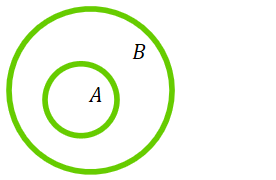
\includegraphics{../Mathematik_1/Bilder/mengen_echte_teilmenge.png} %Diagramm / Beispiel
\end{minipage}
\begin{minipage}{0.7\textwidth}
	\begin{itemize} 
	\item \(A\) ist eine Teilmenge von \(B\): \(A\subseteq B\)
	\item \(B\) ist eine Obermenge von \(A\): \(A\subseteq B\)
	\item \(A\) ist nicht gleich \(B\): \(A\not = B\)
	\item \(A\) ist eine \textbf{echte} Teilmenge von \(B\): \(A\subsetneq B\)
\end{itemize}
\end{minipage}
\end{exabox}
  
Zwei Mengen \(A\) und \(B\) sind gleich, \(A=B\), wenn sie dieselben Elemente enthalten. 

In der Mengenlehre gibt es vier grundlegende Mengenoperationen, n�mlich: Vereinigung, Schnitt, Differenz und Komplement: 

\begin{exabox}{Mengenoperationen}{}
	\begin{itemize}
		\item Die Vereinigung  (\emph{union}) zweier Mengen wird mit dem Symbol \(\cup\) angezeigt. Die Vereinigungsmenge enth�lt jedes Element der beiden Mengen genau einmal, beispielsweise
	\[ \{ 1, 2, 4\} \cup \{2, 5, 3, 4\} = \{1,2,3,4,5\}\,. \]
\item Der Schnitt (\emph{intersection}) zweier Mengen wird mit dem Symbol \(\cap\) angezeigt. Die Schnittmenge enth�lt jedes Element, das in beiden Mengen vorkommt, beispielsweise 
	\[ \{ 1, 2, 4\} \cap \{2, 5, 3, 4\} = \{2,4\}\,. \]
\item Die Differenz (\emph{difference}) zweier Mengen wird mit einem Backslash angezeigt. Die Differenzmenge enth�lt jedes Element, das in der ersten Menge vorkommt, aber nicht in der zweiten, beispielsweise 
	\[ \{ 1, 2, 4\} \setminus \{2, 5, 3, 4\} = \{1\}\,.\]
\item Das Komplement (\emph{complement}) einer Menge \(A\) wird mit einem waagerechten Strich �ber der Menge angezeigt, also \(\overline A\). Ist eine Obermenge \(B\) von \(A\) fixiert, dann bedeutet das Komplement \(\overline A\) die Differenz von Obermenge \(B\) und \(A\). Aus der Schreibweise \(\overline A\) geht die Obermenge nicht hervor - die Obermenge muss also implizit bekannt sein! Im folgenden Beispiel ist die Obermenge die Menge der nat�rlichen Zahlen ohne die Null, also $\mathbb N = \{ 1, 2, 3, 4, 5, 6, \dots\}$: 
	\[ \overline{\{2, 4, 6, 8\}} = \mathbb N \setminus \{2, 4, 6, 8\} = \{1,3,5,7\} \cup \{9,10,11,12, \dots\}\,. \]
	\end{itemize}
\end{exabox}

Neben den bisher betrachteten Mengenoperationen gibt es eine weitere wichtige M�glichkeit, aus gegebenen Mengen eine neue Menge zu bilden. Dabei werden die Elemente der beiden Mengen nicht vereinigt oder miteinander verglichen, sondern zu \textbf{geordneten Paaren} zusammengesetzt.

F�r zwei Mengen \(A\) und \(B\) hei�t

$$
A\times B
=
\{(a,b):a\in A \text{ und } b\in B\}
$$

das kartesische Produkt (\emph{cartesian product}) von \(A\) und \(B\).

Anders als bei den Elementen einer Menge spielt innerhalb eines geordneten Paares die Reihenfolge eine Rolle. Im Allgemeinen gilt daher

$$
(a,b)\neq(b,a).
$$

Das passt zu dem bereits bekannten Unterschied zwischen Mengen und Tupeln: W�hrend beispielsweise

$$
\{2,3\}=\{3,2\}
$$

gilt, sind die geordneten Paare

$$
(2,3)\neq(3,2)
$$

verschieden.

\begin{exabox}{Kartesisches Produkt}{ }
F�r

$$
A=\{\circ,\diamond,M\}
\qquad\text{und}\qquad
B=\{3,7\}
$$

ergibt sich

$$
\begin{aligned}
A\times B
=
\{&
(\circ,3),(\circ,7),
(\diamond,3),(\diamond,7),\\
&
(M,3),(M,7)
\}.
\end{aligned}
$$

Jedes Element aus \(A\) wird dabei mit jedem Element aus \(B\) kombiniert.
\end{exabox}

Besonders wichtig ist das kartesische Produkt einer Menge mit sich selbst. F�r die reellen Zahlen gilt beispielsweise

$$
\mathbb R^2
:=
\mathbb R\times\mathbb R
=
\{(x,y):x\in\mathbb R \text{ und } y\in\mathbb R\}.
$$

Die Elemente von \(\mathbb R^2\) sind also geordnete Paare reeller Zahlen. Sie k�nnen geometrisch als Punkte der Ebene interpretiert werden.

Entsprechend entstehen durch weitere kartesische Produkte geordnete Tripel und allgemein geordnete \(n\)-Tupel. Beispielsweise ist

$$
\mathbb R^3
=
\{(x,y,z):x,y,z\in\mathbb R\}
$$

die Menge aller geordneten Tripel reeller Zahlen und kann als Menge der Punkte des dreidimensionalen Raumes aufgefasst werden.
  
Entsprechend zu "\,Punktrechnung vor Strichrechnung"\, wird der Schnitt vor der Vereinigung ausgef�hrt:
\begin{theorembox}{Rechenregel: Schnitt vor Vereinigung}{ }
$  A \cup B \cap C = A \cup \left( B \cap C\right) \,.  $
\end{theorembox}

\subsection{Was ist eine mathematische Aussage?}

Eine  mathematische Aussage (\emph{statement,  proposition}) ist eine Aussage, der man einen Wahrheitswert zuordnen kann. Entweder ist die Aussage wahr (\emph{true}) oder falsch (\emph{false}). Eine mathematische Aussage kann aus diesem Grund \textbf{keine} freien Variablen enthalten. Wenn freie Variablen vorkommen, handelt es sich um ein Pr�dikat. Man nennt ein Pr�dikat auch "\,eine Aussageform"\, oder einfach "\,ein mathematischer Ausdruck"\,:
  
\begin{exabox}{Aussagen und Pr�dikate}{ }
  \begin{itemize}
  \item "$2^2 = 5$"\, ist eine falsche Aussage.
    \item "$2^2 \not= 5$" \; ist eine wahre Aussage.
    \item "$x^2 \in \mathbb N$" \; ist ein Pr�dikat.
  \end{itemize}
\end{exabox}

  
\begin{exabox}{Aussagen}{ }
  \begin{itemize}
	  \item "\,F�r eine beliebige nat�rliche Zahl $x\in \mathbb N$ gilt $x^2 \in \mathbb N$"\; ist eine wahre Aussage.
	  \item "\,F�r eine beliebige rationale Zahl $x\in \mathbb Q$ gilt  $x^2 \in \mathbb N$"\; ist eine falsche Aussage.
  \end{itemize}
\end{exabox}
Mathematische Aussagen treten selten isoliert auf. H�ufig m�chte man Aussagen \textbf{verneinen} oder mehrere Aussagen miteinander \textbf{verkn�pfen}. Auch daf�r besitzt die Mathematik eine eigene Kurzschreibweise.

Beginnen wir mit der Negation oder Verneinung. Betrachten wir die Aussage

$$
p:\qquad x\geq 0.
$$

Diese Aussage ist beispielsweise f�r \(x=3\) wahr und f�r \(x=-2\) falsch. M�chte man genau das Gegenteil von \(p\) ausdr�cken, so lautet die entsprechende Aussage:

$$
q: \qquad x<0.
$$

In Worten k�nnte man auch sagen: �Es gilt \textbf{nicht} \(x\geq0\).�

Die Aussage \(q\) ist die Negation (\textit{negation}) von \(p\) und das l�sst sich in mathematischer Formelsprache mit Hilfe des Symbols \(\neg\) ausdr�cken: die Negation von \(p\) ist 

$$
\neg p.
$$

Eine Negation \(\neg p\) ist genau dann wahr, wenn die urspr�ngliche Aussage \(p\) falsch ist -- und umgekehrt.

\begin{exabox}{Negation einer Aussage}{ }
	\begin{itemize}
\item F�r $ \; p:\qquad x\geq 0\; $ lautet die Negation $ \;\neg p:\qquad x<0$.
\item Beispielsweise ist f�r \(x=-2\) die Aussage \(p\) falsch und die Aussage \(\neg p\) wahr.
	\end{itemize}
\end{exabox}

Neben der Negation einer einzelnen Aussage m�chte man Aussagen auch miteinander verbinden. Betrachten wir beispielsweise die Aussage \( p:\; x>2\) und die Aussage \(q:\; x<5\). Suchen wir alle reellen Zahlen, f�r die \textbf{sowohl}  \(p\) \textbf{als auch} \(q\) gleichzeitig wahr ist, so verkn�pfen wir die Aussagen durch ein logisches �und�. In mathematischer Formelsprache ist das logische �und� das Symbol \(\land\):

$$
p\land q: \qquad x>2 \;\textnormal{und gleichzeitig} \; x<5.
$$
Eine Und-Verkn�pfung (\emph{and}) \(p\land q \) ist genau dann wahr, wenn sowohl \(p\) als auch \(q\) wahr sind.

Suchen wir alle reellen Zahlen, f�r die \textbf{mindestens eine der Aussagen}, wahr ist, so verkn�pfen wir die Aussagen durch ein logisches �oder� . In mathematischer Formelsprache ist das logische �oder�  das Symbol \(\lor\): 

$$
p\lor q: \qquad x>2 \;\textnormal{oder}\; x<5.
$$
Eine Oder-Verkn�pfung (\emph{or}) \(p\land q \) ist genau dann wahr, wenn  mindestens eine der beiden Aussagen \(p\) und \(q\) wahr ist.

\begin{exabox}{Und und Oder lesen}{ }
	Es seien $ p:\; x>2$ und $q:\; x<5 $.
	\begin{itemize}
		\item $ p\land q $ bedeutet in Worten  �\(x\) ist gr��er als \(2\) und gleichzeitig kleiner als \(5\).� und  diese Aussage ist  genau dann wahr wenn $ 2<x<5 $.  
		\item $ p\lor q $ bedeutet in Worten  �\(x\) ist gr��er als \(2\) oder kleiner als \(5\).� und diese Aussage ist genau dann wahr wenn \(x>2\) oder \(x<5\) wahr ist, wobei auch beide Bedingungen gleichzeitig erf�llt sein d�rfen (aber nicht m�ssen).
	\end{itemize}
\end{exabox}

\noindent{\textbf{Bemerkungen:}}
\begin{itemize}
	\item Die Symbole \(\neg\), \(\land\) und \(\lor\) werden uns immer wieder begegnen. Sie sind nicht nur Bestandteil der Aussagenlogik, sondern geh�ren zur mathematischen Formelsprache. 
	\item Bei der Beschreibung von Mengen werden wir Bedingungen mit diesen Operatoren sinnvoll verkn�pfen. Deshalb ist es wichtig, logische Ausdr�cke nicht nur selbst aufschreiben, sondern auch in nat�rliche Sprache �bersetzen zu k�nnen.
	\item Beim mathematischen Oder ist das Wort �oder� einschlie�lich zu verstehen: Sind \(p\) und \(q\) beide wahr, dann ist auch \(p\lor q\) wahr. Das unterscheidet das mathematische Oder von Formulierungen wie �entweder -- oder�, bei denen h�ufig gemeint ist, dass genau eine von zwei M�glichkeiten eintreten soll.
\end{itemize}

Entsprechend zu �Punktrechnung vor Strichrechnung� gibt es auch f�r logische Operatoren eine festgelegte Reihenfolge: Zuerst wird die Negation ausgef�hrt, danach das Und und zuletzt das Oder.

\begin{exabox}{Klammern weglassen?}{ }
Betrachten wir den vollst�ndig geklammerten Ausdruck

$$
\bigl(\neg(x\geq 6)\bigr)\lor\bigl((x\geq 10)\land(x<20)\bigr).
$$

Welche Klammern k�nnen weggelassen werden, ohne die Bedeutung des Ausdrucks zu ver�ndern?

Da die Negation \(\neg\) vor dem Und \(\land\) und das Und vor dem Oder \(\lor\) ausgef�hrt wird, kann man k�rzer schreiben:

$$
\neg(x\geq6)\lor (x\geq10)\land(x<20).
$$

Die Klammer um \(x\geq6\) bleibt stehen, da sich die Negation auf die gesamte Aussage \(x\geq6\) bezieht.
\end{exabox}

Liest man zwischen zwei Ausdr�cken \(p\) und \(q\) das Symbol $"\Rightarrow"$, dann ist das Konstrukt \( p\Rightarrow q\)  eine logische Schlussfolgerung oder Implikation. Ein Beispiel: 
\begin{exabox}{Schlussfolgerung (Implikation)}{ }
  $ x \geq 7 \Rightarrow x > 5$
\end{exabox}

Mit Worten liest man die Implikation \("p\Rightarrow q"\) wie folgt:
\begin{itemize}
	\item aus $p$ folgt $q$,
	\item wenn $p$ wahr ist, dann ist $q$ wahr,
	\item die G�ltigkeit von $p$ reicht aus \footnote{�fter - aber irgendwie verwirrend - ist hinreichend} (\emph{sufficient}) f�r die G�ltigkeit von \(q\),
\end{itemize}

Es ist wichtig zu bemerken, dass man die Reihenfolge der Ausdr�cke \(p\) und \(q\) in einer Implikation nicht vertauchen darf:
\begin{exabox}{Implikation ist keine kommutative Verkn�pfung}{ }
	Es regnet $\begin{array}{c}\Rightarrow \\\not \Leftarrow\end{array}$ Der Himmel ist bew�lkt.
\end{exabox}



Liest man zwischen zwei Aussagen \(p\) und \(q\) das Symbol \(\Leftrightarrow\), dann handelt es sich um eine �quivalenz. Die Schreibweise

$$
p\Leftrightarrow q
$$

bedeutet, dass \(p\) und \(q\) immer denselben Wahrheitswert besitzen: Entweder sind beide Aussagen wahr oder beide Aussagen sind falsch.\footnote{Das �quivalenzzeichen ist damit f�r die Logik das, was das Gleichheitszeichen \(=\) f�r die Algebra ist.}

�quivalenzen treten beispielsweise beim Umformen von Gleichungen auf. Wird eine Gleichung durch �quiva\-lenz\-umformungen gel�st, dann beschreiben die einzelnen Zeilen jeweils dieselbe L�sungsmenge:

\begin{exabox}{�quivalenz beim L�sen einer Gleichung}{ }

$$
3x-1=2
\quad\Leftrightarrow\quad
3x=3
\quad\Leftrightarrow\quad
x=1
\quad\Leftrightarrow\quad
\mathbb L=\{1\}.
$$

\end{exabox}

Eine �quivalenz kann aber auch zwei unterschiedlich formulierte Aussagen miteinander verbinden:

\begin{exabox}{�quivalenz beim L�sen einer Gleichung}{ }

$$
x^2=4
\quad\Leftrightarrow\quad
x\in\{-2,2\}.
$$

\end{exabox}

Warum darf hier tats�chlich ein �quivalenzpfeil stehen? Daf�r m�ssen beide Richtungen der Aussage gelten.

Von links nach rechts ist zu zeigen:

$$
x^2=4
\quad\Rightarrow\quad
|x|=2
\quad\Rightarrow\quad
x=\pm2
\quad\Rightarrow\quad
x\in\{-2,2\}.
$$

Von rechts nach links ist zu zeigen:

$$
x\in\{-2,2\}
\quad\Rightarrow\quad
x=-2\ \lor\ x=2
\quad\Rightarrow\quad
x^2=4.
$$

Eine �quivalenz

$$
p\Leftrightarrow q
$$

besteht also aus zwei Schlussfolgerungen:

$$
p\Rightarrow q
\qquad\text{und}\qquad
q\Rightarrow p.
$$

Um eine �quivalenz nachzuweisen, m�ssen daher immer beide Richtungen gelten.

Mit Worten liest man die �quivalenz \( p \Leftrightarrow q\) wie folgt: 
\begin{itemize}
  \item $p$ ist genau dann wahr, wenn $q$ wahr ist, 
  \item $p$ gilt dann und nur dann, wenn $q$ gilt (\emph{$p$ if and only if $q$}),
  \item $p$ ist notwendig und hinreichend (\emph{necessary and sufficient}) f�r $q$.  
\end{itemize}

\subsection{Mengen und Aussagen}

Der Gedanke, mit dem wir den Abschnitt eingeleitet haben, klang so, als w�ren Mengen von extremer Bedeutung in der Mathematik: "\,Mengen sind die Grundlage aller mathematischen Objekte."\, Die Mengen, die wir bislang notiert haben, hatten alle weniger als f�nf Elemente und scheinen diese Bedeutung nicht widerzuspiegeln. Mit den Begriffen der Logik haben wir jetzt das Werkzeug an der Hand, um nochmal �ber Mengen nachzudenken und um zu verstehen, dass sie Grundlage der mathematischen Fachsprache sind. 

Was ist eine Menge nochmal? Eine Menge ist eine Ansammlung von Objekten. Kennt man alle Objekte, dann kennt man die Menge - oder anders ausgedr�ckt: man kennt eine Menge, wenn man von einem Objekt sagen kann, ob es zur Menge geh�rt oder nicht. 

Zwei Varianten, die es zulassen zu entscheiden, ob ein Objekt dazugeh�rt oder nicht sind die folgenden: 
\begin{itemize}
	\item Die Menge bzw. deren Elemente sind explizit gegeben. Eine Menge in \textbf{expliziter} Schreibweise lautet beispielsweise so:
\[ M = \{0,1,2,3,4,5,6,7,8,9\}\,, \]
	\item Die Menge wird mit Worten beschrieben. Eine Menge in sogenannter \textbf{intensionaler} Schreibweise lautet beispielsweise so: 
		\[ M = \{ \textnormal{Menge aller nat\"urlichen Zahlen, die kleiner als zehn sind.}\} \]
\end{itemize}
Etwas umst�ndlicher, aber gleichbedeutend ist  
\[ M = \{ \textnormal{Alle Zahlen } \textcolor{blue}{x\,, \textnormal{f\"ur gilt: }} \textcolor{darkgreen}{ x \textnormal{ ist nat\"urlich und } x \textnormal{ ist kleiner als zehn.}}\ \}  \]  
Diese Beschreibung ist zwar verst�ndlich, aber f�r mathematische Texte unn�tig umst�ndlich. Sie l�sst sich unmittelbar in mathematischer Formelsprache �bersetzen. 
\[ M =  \{ \textcolor{blue}{x:} \; \textcolor{darkgreen}{x\in\mathbb N_0 \land x< 10} \}\,. \]  
\begin{itemize}
	\item Das Fragment "\,Alle Zahlen"\,, mit dem die Beschreibung der Menge startet, wurde einfach weggelassen.  
	\item Anstatt "\( x\), f�r die gilt:"\, schreibt man "\( x:\)".\footnote{ manchmal auch "\( x\;|\)".} 
	\item Und "\(x\) ist nat\"urlich und \(x\) ist kleiner als zehn"\, �bersetzt man in mathematische Kurzschreibweise, also "\(x\in\mathbb N_0 \land x<10\)".
\end{itemize}

\noindent{\textbf{ Bemerkungen:}}
\begin{itemize}
	\item Wenn die Menge, die man betrachtet, eine Teilmenge einer bekannten Grundmenge\footnote{\(\mathbb N_0, \mathbb Z, \mathbb Q, \mathbb R, \mathbb C, \cdots\)} ist, beispielsweise eine Teilmenge der nat�rlichen Zahlen, dann schreibt man diese Grundmenge auch oft \textbf{vor} die Zusatzbedingung, also 
\[ M =  \{ x\in \mathbb N_0: x< 10 \}\,. \]  
	\item "\,Bedingung erf�llen"\, bedeutet in der Aussagenlogik, dass eine Aussage wahr wird. Mit Bedingung sind sich all die Eigenschaften gemeint, die die Elemente der Menge haben sollen. 
	\item Oft erf�llen die Elemente einer Menge mehrere Bedingungen und ob die Bedingungen alle gleichzeitig erf�llt sein m�ssen, oder ob eine Bedingung ausreicht, l�sst sich mit Hilfe der Operatoren \(\land\) und \(\lor\) pr�zise angeben.     
\end{itemize}

Mengen beschreibt man also im Allgemeinen mit Hilfe von logischen Ausdr�cken. Hier ein paar Beispiele:
\begin{exabox}{Mengen in mathematischer Kurzschreibweise}{ }
	\begin{itemize}
		\item Die Menge aller reellen Zahlen zwischen $3$ (einschlie�lich) und $5$ (ausschlie�lich)
			\[ M = \{ x \in \mathbb R: x \geq 3 \land x < 5 \} = \{ x \in \mathbb R: 3\leq x < 5 \}\,, \]
		\item Die obere H�lfte der Kreisscheibe ohne Rand. Die Kreisscheibe besitze Radius \(R=1\) und Mittelpunkt \( (0|0)\):
			\[M = \{ (x,y) \in \mathbb R^2: y \geq 0 \land x^2+y^2 < 1\}\,. \]
		\item Streng genommen muss man die Grundmenge angeben, aus der die Elemente zu nehmen sind:
	\[ 
	\begin{array}{rcl}
		\left\{ x \in \mathbb Q: x^2 = 2\right\} &=& \emptyset \,, \\ [1ex]
 \left\{ x \in \mathbb R: x^2 = 2\right\} &=& \left\{ -\sqrt{2}, \sqrt{2} \right\}\,.  
\end{array}
\]
\end{itemize}
\end{exabox}

Um komplexe Konstruktionen solcher Art mathematisch wasserdicht zu machen, muss man von der naiven Mengenlehre zur axiomatischen Mengenlehre �bergehen. Dass ein axiomatischer Zugang n�tig ist, sieht man am Beispiel \href{https://de.wikipedia.org/wiki/Russellsche_Antinomie}{der Russellschen Antinomie }. In der Praxis kommt man mit der naiven Mengenlehre zurecht.

Wenn man Schlussfolgerungen 
\begin{itemize} 
	\item f�r alle Elemente einer Menge treffen m�chte, dann benutzt man in der mathematischen Kurzschreibweise das Symbol $"\forall"$. \(\forall\) ist ein \emph{Quantor} und man �bersetzt ihn mit den Worten "\,f�r alle",
	\item f�r ein Element einer Menge treffen m�chte, dann benutzt man in der mathematischen Kurzschreibweise das Symbol $"\exists"$. \(\exists\) ist ein Quantor und man �bersetzt ihn mit den Worten "\,es existiert (mindestens) ein".
\end{itemize}

\begin{exabox}{Quantoren $\forall$ und $\exists$}{ }
	\begin{itemize}
		\item $A = \{2,4,6\} \; \Rightarrow\; \forall\, x \in A: \dfrac{x}{2} \in \mathbb N^+ .$
		\item $B = \{-3, 2,4,6\} \; \Rightarrow \; \exists\; x \in B: \; x<0 \,.$
	\end{itemize}
\end{exabox}
Ein Quantor hat noch eine weitere wichtige Funktion: Er \textbf{bindet} eine Variable. Betrachten wir beispielsweise das Pr�dikat

$$
p:\qquad x^2\geq 0.
$$

Solange nicht festgelegt ist, f�r welche Zahl \(x\) die Bedingung betrachtet wird, besitzt dieser Ausdruck keinen eigenen Wahrheitswert. Es handelt sich um ein Pr�dikat und noch nicht um eine Aussage.

Erst, wenn man f�r \(x\) einen konkreten Wert annimmt, beispielsweise \(x=-2\), dann entsteht eine Aussage. Beispielsweise ist

$$
p:\qquad (-2)^2\geq0
$$

eine wahre Aussage.

Eine Aussage entsteht aber auch, wenn die Variable durch einen Quantor gebunden wird. So ist

$$
\forall\,x\in\mathbb R:\quad x^2\geq0
$$

eine wahre Aussage. Sie bedeutet: �F�r jede reelle Zahl \(x\) gilt \(x^2\geq0\).�

Auch

$$
\exists\,x\in\mathbb R:\quad x^2=4
$$

ist eine Aussage. Sie bedeutet: �Es gibt mindestens eine reelle Zahl \(x\), f�r die \(x^2=4\) gilt.� Diese Aussage ist ebenfalls wahr.

Ein Pr�dikat wird also zu einer Aussage, wenn f�r die vorkommenden freien Variablen konkrete Werte eingesetzt werden oder wenn die freien Variablen beispielsweise durch Quantoren gebunden werden. Erst dann l�sst sich der entstandenen Aussage eindeutig ein Wahrheitswert zuordnen.

Bei der Negation von Aussagen mit Quantoren ist besondere Vorsicht notwendig. Betrachten wir beispielsweise die Aussage

$$
\text{�Alle Zahlen in der Menge \(M=\{2,4,6,7\}\) sind gerade.�}
$$

Um zu zeigen, dass diese Aussage falsch ist, m�ssen nicht alle Elemente der Menge untersucht und verneint werden. Es gen�gt, ein einziges Element zu finden, das nicht gerade ist. Hier ist \(7\) ein solches Element. Die Negation der Aussage lautet daher:

$$
\text{�Es gibt mindestens eine Zahl in \(M\), die nicht gerade ist.�}
$$

In mathematischer Kurzschreibweise wird aus

$$
\forall\,x\in M:\quad x\text{ ist gerade}
$$

bei der Negation also

$$
\exists\,x\in M:\quad x\text{ ist nicht gerade}.
$$

Die Negation einer Aussage mit dem Quantor \(\forall\) f�hrt zu einer Aussage mit einem Existenzquantor \(\exists\).

Umgekehrt funktioniert derselbe Gedanke. Die Aussage

$$
\text{�Es gibt mindestens eine Zahl in \(M\), die ungerade ist.�}
$$

ist genau dann falsch, wenn keine einzige Zahl in \(M\) ungerade ist. Ihre Negation lautet daher:

$$
\text{�Alle Zahlen in \(M\) sind nicht ungerade.�}
$$

Beim Negieren wird also aus dem Existenzquantor \(\exists\) ein Allquantor \(\forall\) und gleichzeitig wird die zugeh�rige Aussage negiert.

Allgemein gilt:

\begin{theorembox}{Negation quantifizierter Aussagen}{ }

$$
\begin{array}{rcl}
\neg\left(\forall\,x\in M:\;p(x)\right)
&\Leftrightarrow&
\exists\,x\in M:\;\neg p(x),
\\[1ex]
\neg\left(\exists\,x\in M:\;p(x)\right)
&\Leftrightarrow&
\forall\,x\in M:\;\neg p(x).
\end{array}
$$

\end{theorembox}

In Worten bedeutet dies:

$$
\text{�Nicht alle erf�llen \(p\)�}
\quad\Leftrightarrow\quad
\text{�Mindestens eines erf�llt \(p\) nicht�,}
$$

und

$$
\text{�Es gibt keines, das \(p\) erf�llt�}
\quad\Leftrightarrow\quad
\text{�Alle erf�llen \(p\) nicht�.}
$$

\begin{exabox}{Mathematische Kurzschreibweise}{ }
Wie lauten die Definitionen f�r "\,gleiche Mengen"\, oder "\,Mengenoperationen"\, in mathematischer Kurzschreibweise?
	\begin{itemize}
		\item Zwei identische Mengen: \[ A = B: \, \Leftrightarrow\; A\subset B \land B \subset A \;\Leftrightarrow \; \left( \forall \, x \in A: \; x \in B\right) \land \left( \forall \, x \in B: \; x \in A\right)\,. \]
		\item Die Vereinigungsmenge:
			\[  A \cup B = \{ x:\; x \in A \lor x \in B\}\,.\]
		\item Die Schnittmenge:
			\[ A \cap B = \{ x:\; x \in A \land x \in B\}\,. \]
		\item Die Differenzmenge:
			\[ A \setminus B = \{x:\; x\in A \land x \not\in B \}\,. \]
		\item Die Komplementmenge (bei gegebener Menge $B$ und bekannter Obermenge $A$ mit $B\subset A$):
			\[ \overline B = \{ x: x\in A\land x\not \in B\}\,. \]
	\end{itemize}
\end{exabox}

\subsubsection*{Rechenregeln f�r Mengen und Aussagenlogik}

Man kann sagen, dass es zu jedem Mengenoperator einen logischen Operator gibt, der ihm algebraisch entspricht. In der Elektronik muss man logische Operatoren realisieren und das macht man durch Reihen- und/oder Parallelschaltungen. Eine detaillierte �bersicht �ber Logikgatter findet man \href{https://de.wikipedia.org/wiki/Logikgatter}{hier} und die Kurzvariante ist
\begin{center}
  \begin{tabular} {c c c c c }
	  Mengen &  &  Logik & & Elektronik\\
  \hline
  $\cap$ & $ \widehat = $ & $\land$ & $ \widehat = $ & Serie-Schaltung \\
  $\cup$ & $ \widehat = $ &  $\lor$ & $\widehat = $& Parallel-Schaltung\\
  $\overline{\{\}}$ & $ \widehat = $ &  $\neg$ & & \ldots\\
\end{tabular}
\end{center}

Logik "\,unterliegt"\, strengen Gesetzm��igkeiten und wenn man diese kennt, dann wird das "\,logische Argumentieren"\, einfacher:
\begin{theorembox}{Assoziativgesetze und die de Morgansche Gesetze}{ }
  \begin{center}
  \begin{tabular}{c|c|c|c}
  Name & Mengen & Logik & Bedeutung\\
  \hline
  \hline
  \multirow{2}{*}{Assoziativgesetze} & $ (A\cap B) \cap C = A\cap (B \cap C) $ & $ (p \land q) \land r \Leftrightarrow p \land (q \land r)$ & \multirow{2}{*}{ Reihenfolge egal}\\[1ex]
  & $ (A\cup B) \cup C = A\cup (B \cup C) $ & $ (p \lor q) \lor r \Leftrightarrow p \lor (q \lor r)$  & \\[2ex]
  \hline
  \multirow{2}{*}{De Morgansche Gesetze} & $ \overline {A\cap B}  = \overline A\cup  \overline B $ & $  \neg \, ( p \land q)  \Leftrightarrow \neg p \lor \neg q$ & \multirow{2}{*}{Logik der Negation} \\[1ex]
  & $ \overline {A\cup B}  = \overline A\cap  \overline B $ & $  \neg \, ( p \lor q)  \Leftrightarrow \neg p \land \neg q$ &
\end{tabular}
\end{center}
\end{theorembox}

Um die De Morganschen Gesetze zu beweisen, kann man eine Wahrheitstabelle aufstellen! Die Idee ist den logischen Ausdruck $\neg\, (p \land q)$ in Teilaussagen zu zerlegen und dann alle m�glichen F�lle zu betrachten\footnote{Die m�glichen F�lle sind immer  entweder "\,wahr"\, oder "\,falsch"\,, also �berschaubar in Komplexit�t!}: 

\begin{exabox}{Wahrheitstabelle zum Beweis des $1.$ Morganschen Gesetzes}{ }
  \begin{center}
  \begin{tabular}{cc||c|>{\columncolor[gray]{0.9}} c|c|c|>{\columncolor[gray]{0.9}}c} 
	  Input $p$ &  Input $q$ & Output $p\land q$ & Output $\neg (p \land q)$ & Output $\neg p $ & Output $\neg q $ & Output $\neg p \lor \neg q$ \\  
  \hline
  f & f & f & w & w & w & w\\ 
  f & w & f & w & w & r & w\\ 
  w & f & f & w & f & w & w\\ 
  w & w & w & f & f & f & f
\end{tabular}
\end{center}
\end{exabox}
 \newpage % Mengen und Logik                       
\setcounter{exercise}{0} \ifintegriereaufgaben
\section*{Mengen und Aussagenlogik Aufgaben}\label{MA1-mengen-und-logik-aufgaben}

Regeln und Beispiele, die f�r die Bearbeitung der Aufgaben hilfreich sind, finden Sie im Skript\wennreferenzvorhanden{MA1-mengen-und-logik}{ (Abschnitt \abschnittsverweis{MA1-mengen-und-logik})} und, falls Sie nicht weiterkommen, schauen Sie \hyperref[MA1-mengen-und-logik-loesungen]{hier}.

\else
\section{Mengen und Aussagenlogik Aufgaben}\label{MA1-mengen-und-logik-aufgaben}

Regeln und Beispiele, die f�r die Bearbeitung der Aufgaben hilfreich sind, finden Sie im Skrpt und, falls Sie nicht weiterkommen, schauen Sie \hyperref[MA1-mengen-und-logik-loesungen]{hier}. 
\fi

%\begin{exercisebox}[Brainteaser - Logik]
%	Welcher Tag ist morgen, wenn vorgestern der Tag nach Montag war?
%\end{exercisebox}
%
%\begin{exercisebox}[Brainteaser - Logik]
%	Das Einzelkind Matthias steht vor einem �lgem�lde. Er erkl�rt: Der Vater des Abgebildeten ist der Sohn meines Vaters. Wer ist auf dem Gem�lde zu sehen?
%\end{exercisebox}

%\begin{exercisebox}[Schubfachprinzip]
%	Beweisen Sie: Hat man \(n+1\) Objekte in \(n\) Schubladen verteilt, so gibt es mindestens eine Schublade, in der zwei Objekte liegen.
%\end{exercisebox}

%\begin{exercisebox}[M�chtigkeit von unendlichen Mengen]
%	In einem Hotel mit endlich vielen Zimmern k�nnen keine G�ste mehr aufgenommen werden, sobald alle Zimmer belegt sind (Schubfachprinzip). Hilberts Hotel hat nun unendlich viele Zimmer (durchnummeriert mit nat�rlichen Zahlen bei \(1\) beginnend). Man k�nnte nun annehmen, dass dasselbe Problem auch hier auftreten w�rde, n�mlich dann, wenn alle Zimmer durch (unendlich viele) G�ste belegt sind.
%	Es gibt jedoch einen Weg, Platz f�r einen weiteren Gast zu schaffen. Wie k�nnte das gehen?
%\end{exercisebox}

\begin{exercisebox}[Mengen]
	Geben Sie die Mengen explizit an:
	\begin{itemize}
		\item[(a)] $A = \{ x:\; x^2-3x+2 = 0\}$
		\item[(b)] $B = \{ x:\; x \, \textnormal{ist ein Buchstabe aus dem Wort Leipzig} \}$
		\item[(c)] $C = \{ x:\; x^2= 9 \land  x^3=27\}$
		\item[(d)] $D = \{ x:\; x^2= 9 \lor  x -3 =6\}$
		\item[(e)] $E = \{ x:\; x^2= 9 \land  x -3 =6\}$
	\end{itemize}
\end{exercisebox}

\begin{exercisebox}[Mengenoperationen]
	Wie l�sst sich anhand der beiden Mengen $ \mathbb{M}_1 = \{ 1,\, 2,\, 3,\, 4,\, 5,\, 6\}$ und $ \mathbb{M}_2 = \{4,\, 5,\, 6,\, 7,\, 8,\, 9, 10\}$ zeigen, dass bei einer Differenzmenge $\mathbb{M}_1 \setminus \mathbb{M}_2$ die Mengen $\mathbb{M}_1$ und $\mathbb{M}_2$ im Allgemeinen nicht vertauscht werden k�nnen?
\end{exercisebox}

\begin{exercisebox}[Aussagenlogik]
	Negieren Sie die folgenden Ausdr�cke und vereinfachen Sie die Negation so weit wie m�glich und entscheiden Sie, ob die negierte Aussage wahr oder falsch ist. Tipp: Wenden Sie dann die Regeln zur Negation quantorisierter Ausdr�cke und die De Morganschen Gesetze an. 
	\begin{itemize}
		\item[(a)] Alle gut vorbereiteten Studierenden bestehen die Mathematikklausur.
		\item[(b)] Es gibt eine reelle Zahl, die gerade und Teiler von $27$ ist.
		\item[(c)] Alle Zahlen, deren Quersumme durch $3$ teilbar ist, sind durch $3$ teilbar. 
	\end{itemize}
\end{exercisebox}

\begin{exercisebox}[Mengen und Aussagenlogik]
	Seien $A$ und $M$ Mengen. Unter welchen Bedingungen an die Elemente von \(A\) und \(M\) ist $A\not\subseteq M$ eine wahre Aussage?  {Hinweis:} \( A \not \subseteq M \Leftrightarrow \neg\left( A\subset M\right)\).
\end{exercisebox}

\begin{exercisebox}[Aussagenlogik]
Negieren Sie die folgenden Aussagen! Schreiben Sie dabei die Aussagen und ihre Negationen auch mit Quantoren und geben Sie an, ob die Aussage oder ihre Negation wahr ist! 
\begin{itemize}
\item[(a)] Jede nat�rliche Zahl hat einen Vorg�nger.
\item[(b)] Jede nat�rliche Zahl hat einen Nachfolger.
\item[(c)] Es gibt keine reelle Zahl, die zugleich positiv und negativ ist.
\item[(d)] Es gibt keine reelle Zahl, die weder positiv noch negativ ist.
\item[(e)] Jede nichtnegative reelle Zahl ist positiv.
\item[(f)] Die Gleichung $x^2+2x+3=0$ hat eine reelle L�sung.
\item[(g)] Jedes Viereck, das zugleich Rechteck und Drachenviereck ist, ist ein Quadrat.
%\item Jeder Student ist bei der Vorlesung anwesend.
%\item Es gibt einen Studenten, der nicht im Wohnheim wohnt.
\end{itemize}
\end{exercisebox}


\begin{exercisebox}[Brainteaser]
	An einer Weggabelung wohnen zwei Br�der, von denen einer die Angewohnheit hat, stets die Wahrheit zu sagen, w�hrend der andere immer l�gt. Ein Wanderer, der vorbeikommt, m�chte sich nach dem richtigen Weg erkundigen. Er hat von den eigent�mlichen Geschwistern geh�rt, wei� aber nicht, welcher von beiden die Wahrheit sagt. Wie kann er mit nur einer Frage an einen der M�nner herausfinden, welchen Weg er nehmen muss?
\end{exercisebox}
 \newpage
\setcounter{satz}{0} \setcounter{def}{0} \setcounter{exa}{0}  \section{Zahlenmengen}\label{MA1-zahlenmengen}

\begin{table}[H]
  \centering
  \begin{tabularx}{\textwidth}{p{0.9\textwidth} p{0.1\textwidth}}
    \toprule
	  \multicolumn{2}{c}{\textbf{�bersicht �ber Lernziele und Voraussetzungen}}\\
    \midrule
	  \textbf{Lernziele} &\\[.5\normalbaselineskip]
    \tabitem die Zahlenmengen \(\mathbb N_0, \mathbb N^+, \mathbb Z, \mathbb Q\) unterscheiden und korrekt verwenden &\\
    \tabitem die wesentlichen Eigenschaften eines K�rpers am Beispiel von
\(\mathbb Q\) und \(\mathbb R\) erkl�ren & \\
    \tabitem Fakult�ten und Binomialkoeffizienten berechnen &\\
    \tabitem Rechengesetze in \(\mathbb R\) sicher anwenden &\\
    \tabitem Summen- und Produktsymbole ausschreiben und vereinfachen &\\
    \tabitem den Binomischen Satz anwenden &\\
    \midrule
	  \textbf{Voraussetzungen} \\[.5\normalbaselineskip]
    \tabitem Grundrechenarten &\\
    \bottomrule
  \end{tabularx}
\end{table}

\ifintegriereaufgaben \noindent �bungsaufgaben zum Thema finden Sie hier: \hyperref[MA1-zahlenmengen-aufgaben]{Aufgaben}
\vspace{0.3cm}
\hrule
\fi

\subsection{Nat�rliche, ganze und rationale Zahlen}

Zum Z�hlen ben�tigt man die Zahlen $1,  2,  3,\dots$. Diese Menge von Zahlen nennt man die \textbf{nat�rlichen Zahlen} (\emph{natural numbers}) und f�hrt das Symbol \(\mathbb N\) ein. Allerdings ist unklar, ob \(\mathbb N\) die Null beinhaltet oder nicht\footnote{In der Informatik z�hlt die Null meist dazu und in der Mathematik mal so mal so.} In diesem Skript werden Indizes eingef�hrt, die die Frage pr�zise kl�ren: $\mathbb N_0$ enth�lt die Null und $\mathbb N^+$ nicht.\footnote{Wie lauten die Bedingungen in mathematischer Kurzschrift? \(0\in \mathbb N_0\) und \( \forall n\in \mathbb N^+: n>0\).}

Im Zahlenbereich $\mathbb Z$ der  \textbf{ganzen Zahlen}  (\emph{integers}) kommen die negativen ganzen Zahlen hinzu. 

Kommen noch alle positiven und negativen Br�che hinzu, erh�lt man den Bereich der \textbf{rationalen Zahlen} \(\mathbb Q\) (\emph{rational numbers}).

\begin{defbox}{Nat�rliche, ganze und rationale Zahlen: $\mathbb N$, $\mathbb Z$ und $\mathbb Q$}{ }
\begin{eqnarray*}
	\mathbb N_0 &=& \{ 0,1,2,3, 4\dots \}\,, \\
	\mathbb N^+ &=&  \{ 1,2,3, 4\dots \}\,, \\
	\mathbb Z &=& \left\{ \dots,-3,-2,-1,0,1,2,3,\dots \right\} = \mathbb N_0 \cup \{-1,-2,-3,-4,\cdots\}\,,\\
   \mathbb Q &=& \left\{ \displaystyle{\frac{m}{n}}, \quad m \in \mathbb Z \land n \in \mathbb N^+\right\}\,.
  \end{eqnarray*}
\end{defbox}

Wenn eine Rechenoperation in der Mathematik immer wieder auftaucht, dann ist es sinnvoll ein Symbol einzuf�hren. Solche zwei Rechenoperationen mit nat�rlichen Zahlen sind die Fakult�t und der Binomialkoeffizient.\marginpar{\small Aufgabe} Sie sind wie folgt definiert:   

\begin{defbox}{Fakult�t und Binomialkoeffizient}{ }
	\begin{center}
	\begin{tabular}{l|l|l|l}
Name & Symbol & Wertebereich &  Besonderheit  \\
\hline
Fakult�t & \(n! = n\cdot (n-1) \cdot (n-2)  \dots  1 \) & \(n\in \mathbb N_0\) &  \(0! = 1! = 1\) \\[2ex]
Binomialkoeffizient &  \(\displaystyle{\binom{n}{k}} = \displaystyle{\frac{ n!}{ k!\cdot (n-k)!}} \) & \( n,k\in\mathbb N_0 : \;k\leq n \)    & \( \displaystyle{\binom{n}{0}} = \displaystyle{\binom{n}{n}} = 1  \)
\end{tabular}
\end{center}
\end{defbox}

\noindent {\textbf{ Bemerkungen: }}
\begin{itemize}
	\item Die Anzahl der M�glichkeiten $n$ verschiedene Objekte in einer Reihe anzuordnen ist \(n\)-Fakult�t.
	\item Die Anzahl der M�glichkeiten aus einer $n$-elementigen Menge $k$ Elemente auszuw�hlen ist \(n\) �ber \(k\).
\end{itemize}

\subsection{Reelle Zahlen}


Um $x^{2}=2$ l�sen zu k�nnen oder den Umfang eines Kreises mit Durchmesser $1$ als Zahl anzugeben, ben�tigt man einen gr��eren Zahlenbereich: den der \textbf{reellen Zahlen} $\mathbb R$ (\emph{real numbers}). 

\begin{exabox}{Reelle Zahlen}{ }
	$\displaystyle{\left\{-\ln(77)\,, \; \sqrt{2}\,, \; \pi\,, \; \frac{4}{28}\,, \; 38624983 \right\} \subset \mathbb R\,. }$
\end{exabox}

Die reellen Zahlen besitzen gegen�ber den rationalen Zahlen eine weitere wichtige Eigenschaft: Sie sind \textbf{vollst�ndig}\footnote{Vereinfacht gesprochen bedeutet die Vollst�ndigkeit von \(\mathbb R\): Konvergente N�herungsverfahren, deren Werte reelle Zahlen sind und die sich immer weiter auf einen Wert festlegen, f�hren nicht aus dem Zahlenbereich \(\mathbb R\) hinaus.} Anschaulich bedeutet dies, dass der reelle Zahlenstrahl keine �L�cken� besitzt. Eine solche L�cke tritt beispielsweise auf, wenn man versucht, \(\sqrt{2}\) ausschlie�lich mit rationalen Zahlen zu erfassen. Durch immer genauere rationale N�herungen kann man sich der Zahl \(\sqrt{2}\) beliebig weit ann�hern. Der Grenzwert dieser N�herungen ist jedoch selbst keine rationale Zahl. Innerhalb von \(\mathbb Q\) fehlt also genau die Zahl, auf die die N�herungen zulaufen.

\begin{exabox}{Die Zahl \(\sqrt{2}\)}{ }
Ein klassisches Beispiel f�r eine reelle Zahl, die nicht rational ist, ist \(\sqrt{2}\). Angenommen, es g�be einen vollst�ndig gek�rzten Bruch

$$
\sqrt{2}=\frac pq,\qquad p,q\in\mathbb N^+.
$$

Dann folgt

$$
	\begin{array}{rcrcl l} 
		\sqrt{2}=\dfrac pq & \Rightarrow & 2\cdot q^2 &=& p^2 & \Rightarrow p^2\text{ gerade}, p\text{ gerade}\\
		&\Rightarrow & \exists \, k \in \mathbb N^+: \,  p &=& 2\cdot k \\
		&\Rightarrow & 2\cdot q^2=&=& 4\cdot k^2 & \\  & \Leftrightarrow & q^2 &=& 2 \cdot k^2  &\Rightarrow q^2\text{ gerade}, \, q\text{ gerade}.
\end{array}
$$

Damit sind \(p\) und \(q\) beide durch \(2\) teilbar -- im Widerspruch zur Annahme, dass \(p/q\) vollst�ndig gek�rzt ist. Also gilt

$$
\sqrt{2}\notin\mathbb Q.
$$

Trotzdem l�sst sich \(\sqrt{2}\) durch rationale Zahlen beliebig genau eingrenzen:

$$
1<\sqrt{2}<2,\qquad
1{,}4<\sqrt{2}<1{,}5,\qquad
1{,}41<\sqrt{2}<1{,}42,\quad\dots
$$

Es entstehen ineinander geschachtelte Intervalle mit rationalen Grenzen, die \(\sqrt{2}\) immer genauer festlegen. Dieses Verfahren hei�t \textbf{Intervallschachtelung}.
\end{exabox}

Ein zusammenh�ngendes St�ck der reellen Zahlen nennt man ein Intervall. Es gibt offene, halboffene oder abgeschlossene Intervalle -- je nachdem ob beide, nur eines oder beide Intervallenden dazugeh�ren oder nicht. M�chte man ein Intervall aufschreiben, das bis ins Unendliche geht, dann benutzen wir f�r plus Unendlich das Unendlichkeitsymbol $\infty$ und f�r minus Unendlich entsprechend \(-\infty\).\footnote{Aufpassen: Unendlich ist keine reelle Zahl, sondern ein Symbol!} 
\begin{exabox}{Intervalle}{ }
  \begin{itemize}
    \item $[0,1] = \{x\in \mathbb R: 0 \leq x \leq 1\}$,
    \item $(0,1] = \{x\in \mathbb R: 0 < x \leq 1\}$,
    \item $(0,1) = \{x\in \mathbb R: 0 < x < 1\}$,
    \item $(-\infty ,1) = \{x\in \mathbb R: x < 1\}$,
    \item $(-\infty ,+\infty) = \mathbb R$.
  \end{itemize}
\end{exabox}

Eine abschlie�ende Bemerkung: viele reelle Zahlen haben zwei Schreibweisen - schauen Sie sich das an: \[\displaystyle{ 1 = 3\cdot \frac13 = 3 \cdot 0,\bar 3 = 0,\bar 9 \,.}\]

\subsection{Rechenregeln}

In den bisher genannten Zahlenbereichen gelten diese Regeln:  
\begin{theorembox}{Addition und Multiplikation}{ }
\begin{itemize}
  \item Die Addition ist assoziativ: \quad $a+ (b+c) = (a+b)+c $.
  \item Die Multiplikation ist assoziativ: \quad $a\cdot (b\cdot c) = (a \cdot b) \cdot c$.
  \item Die Addition ist kommutativ:\quad $a+b = b+a$.
  \item Die Multiplikation ist kommutativ:\quad $a\cdot b = b \cdot a$
  \item Es gilt das Distributivgesetz: \quad $a \cdot (b+c) = a \cdot b  +  a \cdot c = (b+c) \cdot a = b \cdot a + c \cdot a$.
\end{itemize}
\end{theorembox}

Subtraktion und Division sind dagegen weder assoziativ noch kommutativ!
\begin{exabox}{H�ufige Fehler}{ }
\begin{itemize}
  \item Die Subtraktion ist nicht assoziativ: \quad $3-(4+6)= -7 \not= (3-4)+6 = 5 $.
  \item Die Subtraktion ist nicht kommutativ: \quad $3-4 = -1 \not= 4-3 = 1 $.
  \item Die Division ist nicht distributiv: \quad $25 : ( 5 + 25)  = 25:30 = 5:6 \not= 25:5 + 25:25 = 6 $.
  \item Die Division ist nicht kommutativ: \quad  $5:25 = 1:5 \not= 25:5 = 5 $.
\end{itemize}
\end{exabox}

Die Zahlenbereiche $\mathbb{Q}$ und $\mathbb{R}$ besitzen eine wichtige zus�tzliche Eigenschaft,
die $\mathbb{N}_0$ und $\mathbb{Z}$ nicht haben:

In $\mathbb{Q}$ und $\mathbb{R}$ kann man durch jede von $0$ verschiedene Zahl teilen.

Der Grund daf�r ist, dass zu jeder Zahl $a\neq 0$ eine Zahl $a^{-1}$ existiert,
so dass

\[
a \cdot a^{-1} = 1.
\]

Diese Zahl nennt man das \textbf{multiplikative Inverse} von $a$.
Division durch $a$ entspricht also der Multiplikation mit $a^{-1}$:

\[
\frac{b}{a} = b \cdot a^{-1}.
\]

In den nat�rlichen Zahlen $\mathbb{N}_0$ oder den ganzen Zahlen $\mathbb{Z}$ ist
dies im Allgemeinen nicht m�glich. Die Gleichung 

\[
2 \cdot x = 1
\]

hat keine L�sung in $\mathbb{Z}$ - die L�sung \(x = \frac12\) ist eine rationale Zahl. 

In den Zahlenbereichen $\mathbb{Q}$ und $\mathbb{R}$ gelten die �blichen Rechenregeln (Assoziativ-, Kommutativ- und Distributivgesetz), und jede von $0$ verschiedene Zahl besitzt ein multiplikatives Inverses.  Deshalb kann man in diesen Zahlenbereichen beliebig addieren, subtrahieren, multiplizieren und durch von $0$ verschiedene Zahlen teilen.

Die Zahlenbereiche \(\mathbb Q\) und \(\mathbb R\) besitzen damit eine gemeinsame algebraische Struktur: Beide sind sogenannte \textbf{K�rper} (\emph{fields}). Der Begriff fasst genau die Eigenschaften zusammen, die f�r das Rechnen mit Addition, Subtraktion, Multiplikation und Division ben�tigt werden.

\begin{defbox}{K�rper}{ }
Eine Menge \(\mathbb K\) mit einer Addition \(+\) und einer Multiplikation \(\cdot\) hei�t K�rper, wenn f�r alle \(a,b,c\in\mathbb K\) gilt:

\begin{itemize}
\item Die Addition und die Multiplikation sind assoziativ und kommutativ.
\item Es gibt neutrale Elemente \(0,1\in\mathbb K\) mit \(0\neq1\), sodass f�r all \(a\in \mathbb K\) gilt
\[
a+0=a
\qquad\text{und}\qquad
a\cdot1=a.
\]
\item Zu jedem \(a\in\mathbb K\) gibt es ein additives Inverses \(-a\in\mathbb K\).
\item Zu jedem \(a\in\mathbb K\setminus\{0\}\) gibt es ein multiplikatives Inverses \(a^{-1}\in\mathbb K\).
\item Addition und Multiplikation sind durch das Distributivgesetz miteinander verbunden:

$$
a\cdot(b+c)=a\cdot b+a\cdot c.
$$

\end{itemize}
\end{defbox}

Entscheidend ist dabei, dass die Ergebnisse der Rechenoperationen wieder im selben Zahlenbereich liegen. 

Im Unterschied zu \(\mathbb Q\) ist \(\mathbb R\) vollst�ndig. Die Begriffe \textbf{K�rper} und \textbf{Vollst�ndigkeit} beschreiben also unterschiedliche Eigenschaften eines Zahlenbereichs.

Der Begriff des K�rpers wird sp�ter bei der Definition eines Vektorraums wieder auftreten: Die Skalare, mit denen Vektoren multipliziert werden, stammen aus einem K�rper \(\mathbb K\). In diesem Skript wird dabei meist \(\mathbb K=\mathbb R\) gelten.

\subsubsection*{Summen- und Produktzeichen}

Die Liste an mathematischen Symbolen, die man aus Effizienzgr�nden einf�hrt, erweitern wir noch um das Summen- und das Produktzeichen.\marginpar{Aufgabe} 

	Es sei \(f_k\) ein mathematischer Ausdruck, der von der Variable \(k\) abh�ngt. Mit \(f_1\) ist dann gemeint: setze in dem mathematischen Ausdruck  \(k=1\), mit \(f_a\) ist entsprechend \(k=a\) zu setzen.
\begin{defbox}{Summen- und Produktzeichen}{ }
	\begin{center}
	\begin{tabular}{l|l|l }
Name & Symbol & Wertebereich  \\
\hline
Summenzeichen & \(\displaystyle{ \sum_{k=a}^b} f_k = f_a + f_{a+1} + \dots + f_b \) &  \(f_k \in \mathbb R, \; a\leq b \in \mathbb N_0\) \\[2ex] 
Produktzeichen & \(\displaystyle{ \prod_{k=a}^b} f_k = f_a \cdot f_{a+1} \cdot \dots \cdot f_b \) &  \(f_k\in \mathbb R, \, a\leq b \in \mathbb N_0\) 
\end{tabular}
\end{center} 
\end{defbox}

\begin{exabox}{Summen- und Produktzeichen}{ }
	\begin{eqnarray*} 
		\sum\limits_{k=3}^{6} (1+k)^{k-1} &=& (1+3)^{3-1} + (1+4)^{4-1} + (1+5)^{5-1}+ (1+6)^{6-1} = 4^2+5^3+6^4+7^5 \,,\\
		\prod\limits_{k=1}^{3} x^k &=& x\cdot x^2\cdot x^3 = x^{6}\,.
	\end{eqnarray*}
\end{exabox}

Ein "Binom"\, ist in der Mathematik ein Ausdruck der Form \( (a+b)^n\). Der nun folgende Binomische Satz erkl�rt, warum der Binomialkoeffizient und die aus der Schule bekannten Binomischen Formeln nicht nur scheinbar zusammengeh�ren.\marginpar{Aufgabe}

\begin{theorembox}{Binomischer Satz}{ }
	$$\forall \, a,b\in\mathbb R, \; n\in \mathbb N_0:\quad  (a+b)^n = \sum\limits_{k=0}^{n} \binom{n}{k} a^k \cdot  b^{n-k}$$
\end{theorembox}
 \newpage % Zahlen
\setcounter{exercise}{0} \ifintegriereaufgaben

\section*{Zahlenmengen Aufgaben}\label{MA1-zahlenmengen-aufgaben}

Regeln und Beispiele, die zur Bearbeitung der Aufgaben hilfreich sind, finden Sie im Skript\wennreferenzvorhanden{MA1-zahlenmengen}{ (Abschnitt \abschnittsverweis{MA1-zahlenmengen})} und, falls Sie nicht weiterkommen, schauen Sie \hyperref[MA1-zahlenmengen-loesungen]{hier}.
\else 
\section{Zahlenmengen Aufgaben}\label{MA1-zahlenmengen-aufgaben}

Regeln und Beispiele, die zur Bearbeitung der Aufgaben hilfreich sind, finden Sie im Skript und, falls Sie nicht weiterkommen, schauen Sie \hyperref[MA1-zahlenmengen-loesungen]{hier}.
\fi 

\begin{exercisebox}[K�rperaxiome]
Welche Rechenregeln erf�llen die ganzen Zahlen $\mathbb Z$ nicht im Vergleich zu $\mathbb R$?
\end{exercisebox}


\begin{exercisebox}[Summen- und Produktzeichen]% Definition Summe und Produkt. Rechenregeln.
	Schreiben Sie die folgenden Summen aus und berechnen Sie ihren Wert:
	\begin{equation}
		\begin{array} { lllll }
			(a) \; \displaystyle{\sum\limits_{i=1}^{7} i} & \quad  \quad (b)\; \displaystyle{\prod\limits_{i=1}^{2}} i &\quad \quad (c) \;\displaystyle{\prod\limits_{i=0}^{5}} i &\quad \quad (d)\; \displaystyle{\sum\limits_{i=1}^{5} i^2} &\quad\quad (e)\; \displaystyle{\sum\limits_{i=-3}^{3} i^2} \\
			(f)\; \displaystyle{\prod\limits_{i=-3}^{3}} i^2 &\quad \quad (g)\; \displaystyle{\sum\limits_{i=0}^{7} 5} &\quad \quad (h)\; \displaystyle{\prod\limits_{i=0}^{7}} 2 &\quad \quad (i)\; \displaystyle{\sum\limits_{i=3}^{9} (i-2)} &\quad \quad (j)\; \displaystyle{\prod\limits_{i=-1}^{3}} (i+2)
	\end{array}
\end{equation}
\end{exercisebox}

\begin{exercisebox}[Summenzeichen Indexverschiebung]
	Wie lautet das Argument f�r folgende Indexverschiebung?
	$\displaystyle{\sum\limits_{i=k}^l x_i} = \displaystyle{\sum\limits_{i=k+a}^{l+a}} \textnormal{???} $
\end{exercisebox}

\begin{exercisebox}[Summen- und Produktzeichen]
	Ersetzen Sie in den folgenden Gleichungen die Fragezeichen: % Definition Summe und Produkt. Rechenregeln.
	\begin{eqnarray*}
		\begin{array}{ll}
			(a) \;\; 1+x+\displaystyle{\frac{x^2}{2!}}+\displaystyle{\frac{x^3}{3!}}+\dots\displaystyle{\frac{x^n}{n!}} = \displaystyle{\sum\limits_{i=1}^{\textnormal{?}} \textnormal{?}}  = \displaystyle{\sum\limits_{i=-2}^{\textnormal{?}} \textnormal{?}}  &\quad \quad
			(b)\;\; \displaystyle{\sum\limits_{i=0}^{n}} x^{0\cdot i} = \textnormal{?} \\
			(c)\;\; 1+x+\displaystyle{\frac{x^2}{2!}}+\displaystyle{\frac{x^3}{3!}}+\dots\displaystyle{\frac{x^n}{n!}} =\textnormal{?} \cdot\displaystyle{\sum\limits_{i=0}^{\textnormal{?}}} \frac{x^{i-1}}{i!} &  \quad \quad  (d)\;\; \displaystyle{\frac{\displaystyle{\prod\limits_{i=1}^{n}} 4^i}{\displaystyle{\prod\limits_{i=2}^{n+1}} 2^i}} = \textnormal{?}
	\end{array}
	\end{eqnarray*}
\end{exercisebox}

\begin{exercisebox}[Binomialkoeffizient]
	Zeigen Sie
	$$\binom{n+1}{k} = \binom{n}{k}+ \binom{n}{k-1}, \; k\geq 1\,.$$
\end{exercisebox}

\begin{exercisebox}[Binomischer Satz]
	Bestimmen Sie mithilfe des Binomischen Satzes eine Formel f�r $(a-b)^n$.
\end{exercisebox}

\begin{exercisebox}[Binomischer Satz]
	Zeigen Sie
	$$\sum\limits_{k=0}^n \binom{n}{k} = 2^n$$
\end{exercisebox}

%\begin{exercisebox}[Rechenspiele]
%	Sie sollen die Zahlen \(21\) aus den Zahlen \(1,5,6\) und \(7\) errechnen. Alle diese Zahlen m�ssen in der Gleichung genau einmal vorkommen. Sie d�rfen nur die vier Grundrechenarten \((+,-,\cdot,:)\) sowie Klammern verwenden. Rechnen Sie nur mit ganzen Zahlen. Also zum Beispiel \( 1+5+6+7 = 19\) oder \(5\cdot(7-6+1) = 10\). 
%\end{exercisebox}
%
%\begin{exercisebox}[Vorstellungsgespr�ch]
%	In einem Vorstellungsgespr�ch bietet Ihnen der Personalchef folgendes Spiel an: "Wir addieren ausgehend von der Zahl zehn immer abwechselnd eine Zahl zwischen eins und zehn auf die neue Summe. Wer am Ende auf genau \(100\) addiert hat gewonnen. Ich fange an, um Ihnen das zu demonstrieren: Also \(10+2=12\). Das ist mein erster Zug. Nun ist es an Ihnen." K�nnen Sie das Spiel gewinnen? 
%\end{exercisebox}


%\begin{exercisebox}[Binomialkoeffizient]
%	Auf einer internationalen Konferenz treffen sich Vertreter mit $10$ unterschiedlichen Landessprachen. Wie viele Dolmetscher werden ben�tigt, wenn f�r jede �bersetzung zwischen zwei Sprachen ein eigener Dolmetscher anwesend sein soll?
%\end{exercisebox}

%\begin{theorembox}[Rundungsregeln]
%	\begin{itemize}
%		\item Ist die erste weggelassene Ziffer $0,1,2,3$ oder $4$, so bleibt die letzte geschriebene Ziffer unver�ndert (Abrunden).
%		\item Ist die erste weggelassene Ziffer $5,6,7,8$ oder $9$, so wird die letzte geschriebene Ziffer um eins erh�ht (Aufrunden).
%	\end{itemize}
%\end{theorembox}

%\begin{exercisebox}[Terme vereinfachen]
%	Vereinfachen Sie so weit wie m�glich:
%	%\begin{itemize}
%		%\item $a(c+b)-c(b+a)+b(c-a)$
%		%\item $a(c+b(a-c))-c(b(a-1)+a)-b(c-a(b-a))$
%		%\item $(2b-3a)(3a-2b)-(2a-b)^2$
%		%\item $\displaystyle{\frac{x+3}{x^2-4} + \frac{x-3}{x-2}}$
%		%\item $\left( \displaystyle{\frac{a^3x^5}{a^{-29x^3}}}\right)^4$ % Potenzregeln
%	%\end{itemize}
%\end{exercisebox}
%\begin{theorembox}[Binomische Formeln]
%	F�r alle $a,b$ gilt:
%	\begin{eqnarray*}
%		(a+b)^2 &=& a^2+2ab+b^2\\
%		(a-b)^2 &=& a^2-2ab+b^2\\
%		(a+b)(a-b) &=& a^2-b^2
%	\end{eqnarray*}
%\end{theorembox}

%\begin{theorembox}[Satz von Vieta]
%	Es gelte $\quad x^2+ax+b= (x+p)(x+q)$ f�r alle $x\in \mathbb R$. Welche Beziehungen m�ssen dann zwischen $a, b$ und $p,q$ gelten?
%	$\forall x\in \mathbb R: \quad x^2+ax+b= (x+p)(x+q)\; \Leftrightarrow \; a=p+q \land b=pq \,.$
%\end{theorembox}
 \newpage  
\setcounter{satz}{0} \setcounter{def}{0} \setcounter{exa}{0}  \section{�quivalenzumformungen (+)}\label{MA1-aequivalenzumformungen}

\begin{table}[H]
  \centering
  \begin{tabularx}{\textwidth}{p{0.9\textwidth} p{0.1\textwidth}}
    \toprule
	  \multicolumn{2}{c}{\textbf{�bersicht �ber Lernziele und Voraussetzungen}}\\
    \midrule
	  \textbf{Lernziele} &\\[.5\normalbaselineskip]
    \tabitem lineare und quadratische Gleichungen l�sen &\\
    \tabitem lineare und quadratische Ungleichungen systematisch bearbeiten &\\
    \tabitem Betragsungleichungen und Bruchungleichungen l�sen &\\
    \tabitem lineare und quadratische Ungleichungen systematisch bearbeiten &\\
    \midrule
	  \textbf{Voraussetzungen} \\[.5\normalbaselineskip]
	  \tabitem Mengenoperationen und Intervallschreibweisen & \abschnittsverweis{MA1-mengen-und-logik}\\
	  \tabitem Grundrechenarten & \abschnittsverweis{MA1-zahlenmengen}\\
	  \tabitem �quivalenzumformungen & \abschnittsverweis{MA1-aequivalenzumformungen}\\
    \bottomrule
  \end{tabularx}
\end{table}

\ifintegriereaufgaben \noindent �bungsaufgaben zum Thema finden Sie hier:  \hyperref[MA1-aequivalenzumformungen-aufgaben]{Aufgaben}
\vspace{0.3cm}
\hrule
\fi

\subsection{�quivalenzumformungen und L�sungsmenge}

Beim Umformen von Gleichungen und Ungleichungen ersetzen wir einen Ausdruck durch einen logisch �quivalenten,
aber einfacheren Ausdruck. Ziel ist eine Beschreibung aller Zahlenwerte, f�r die die Aussage wahr ist.
Diese Menge nennt man \textbf{L�sungsmenge}.

\begin{exabox}{L�sungsmenge einer linearen Gleichung}{ }
	\[
	4\, x+7=0 
	\;\Leftrightarrow\;
	x\in \mathbb L=\{x\in\mathbb R:\;4\, x+7=0\}
	=
	\left\{-\frac74\right\}.
	\]
\end{exabox}

\noindent \textbf{Bemerkungen:}
\begin{itemize}
	\item Nie durch Null dividieren und nie mit Null multiplizieren. Problemstellen m�ssen ausgeschlossen
	und ggf. separat betrachtet werden:
	\[
	\frac{x-3}{x+2}=10
	\stackrel{x\neq -2}{\Leftrightarrow}
	x-3=10\cdot(x+2)
	\Leftrightarrow
	x=-\frac{23}{9}.
	\]
\item Nicht jede Gleichung ist mit dem bisherigen Werkzeug direkt l�sbar (z.\,B.\ Gleichungen, in denen trigonometrische Funktionen auftauchen).\wennreferenzvorhanden{MA1-potenz-und-wurzelfunktionen}{\wennreferenzvorhanden{MA1-trigonometrische-funktionen}{\marginpar{ \small {\abschnittsverweis{MA1-potenz-und-wurzelfunktionen}--\abschnittsverweis{MA1-trigonometrische-funktionen}}}}}
\end{itemize}

Auch bei Ungleichungen ist das Ziel eine L�sungsmenge, oft ein Intervall oder eine Vereinigung von Intervallen.

\begin{exabox}{L�sen einer linearen Ungleichung}{ }
	\[
	2\, x+6\le 2
	\;\Leftrightarrow\;
	x\le -2
	\;\Leftrightarrow\;
	x\in(-\infty,-2].
	\]
\end{exabox}
Das L�sen einer Ungleichung funktioniert damit zun�chst ganz �hnlich wie das L�sen einer Gleichung: Beide Seiten d�rfen getrennt vereinfacht werden, und auf beiden Seiten darf derselbe Term addiert oder subtrahiert werden. So kann eine Ungleichung Schritt f�r Schritt in eine einfachere, aber �quivalente Form gebracht werden.

Beim Multiplizieren und Dividieren ist allerdings das \textbf{Vorzeichen} des verwendeten Faktors entscheidend. Wird eine Ungleichung mit einer positiven Zahl multipliziert oder durch eine positive Zahl dividiert, bleibt die Richtung des Ungleichheitszeichens erhalten. Beispielsweise gilt

$$
2<5
\qquad\Longleftrightarrow\qquad
2\cdot 3<5\cdot 3.
$$

Bei einer negativen Zahl kehrt sich dagegen die Richtung des Ungleichheitszeichens um:

$$
2<5
\qquad\Longleftrightarrow\qquad
2\cdot(-3)>5\cdot(-3).
$$

Der Grund daf�r wird bereits am Ergebnis sichtbar:

$$
-6>-15.
$$

F�r das systematische Umformen einer Ungleichung gelten damit folgende Regeln:
\begin{enumerate}
\item Beide Seiten der Ungleichung d�rfen jeweils durch �quivalente Terme ersetzt werden. Dazu geh�ren beispielsweise das Ausmultiplizieren, Faktorisieren oder Zusammenfassen von Termen.

\item Auf beiden Seiten darf derselbe Term addiert oder subtrahiert werden:
\[
T_1<T_2
\;\Leftrightarrow\;
T_1+T<T_2+T.
\]

\item Beide Seiten d�rfen mit demselben von Null verschiedenen Term multipliziert oder durch ihn dividiert werden. Dabei muss dessen Vorzeichen ber�cksichtigt werden:
\[
\begin{array}{rcl}
T_1<T_2\ \land\ T>0
&\Leftrightarrow&
T_1\cdot T<T_2\cdot T,
\\[1ex]
T_1<T_2\ \land\ T<0
&\Leftrightarrow&
T_1\cdot T>T_2\cdot T.
\end{array}
\]
Entsprechendes gilt f�r die Division durch \(T\neq0\).

\end{enumerate}

Besonders wichtig ist die dritte Regel, sobald mit einem Term multipliziert oder durch einen Term dividiert wird, dessen Vorzeichen von der Variablen abh�ngt. Ist beispielsweise der Faktor \(x-2\), so ist dieser f�r \(x>2\) positiv und f�r \(x<2\) negativ. In solchen Situationen muss zun�chst unterschieden werden, welches Vorzeichen der Faktor besitzt. Genau daraus entstehen die \textbf{Fallunterscheidungen}, die beim L�sen vieler Ungleichungen eine zentrale Rolle spielen.


\subsection{Strukturiertes L�sen von Ungleichungen}

Der Umgang mit �quivalenzumformungen und das saubere Aufschreiben von L�sungsmengen l�sst sich besonders gut an algebraischen Ungleichungen trainieren. Im Folgenden werden drei typische Formen betrachtet:
\begin{enumerate}
\item quadratische Ungleichungen,
\item Bruchungleichungen,
\item Betragsungleichungen.
\end{enumerate}

Diese Ungleichungen sehen zun�chst sehr unterschiedlich aus. Das Vorgehen beruht jedoch immer wieder auf derselben Idee: Durch eine sinnvolle \textbf{Fallunterscheidung} wird die urspr�ngliche Ungleichung auf einfachere Ungleichungen zur�ckgef�hrt. Die folgenden Beispiele zeigen dieses Vorgehen Schritt f�r Schritt.
\marginpar{\small Aufgaben}

Wenn auf beiden Seiten des Ungleichheitszeichens quadratische Ausdr�cke derselben Variablen stehen, k�nnen zun�chst alle Terme auf eine Seite gebracht werden. Anschlie�end wird untersucht, f�r welche Werte der entstehende quadratische Term positiv oder negativ ist.

\begin{exabox}{L�sen einer quadratischen Ungleichung}{ }
Betrachtet wird die Ungleichung

$$
2x^2+x-4>x^2+6x-10.
$$

Die L�sung l�sst sich systematisch in mehreren Schritten bestimmen.

\begin{enumerate}
\item Zun�chst werden alle Terme auf eine Seite gebracht:

$$
2x^2+x-4>x^2+6x-10
\;\Leftrightarrow\;
x^2-5x+6>0.
$$

\item Der quadratische Term wird in Linearfaktoren zerlegt:

$$
x^2-5x+6=(x-2)(x-3).
$$

Damit ist zu untersuchen, wann

$$
(x-2)(x-3)>0
$$

gilt.

\item Ein Produkt ist positiv, wenn beide Faktoren positiv oder beide Faktoren negativ sind. Daher m�ssen zwei F�lle unterschieden werden:

$$
\begin{array}{rcl}
(x-2)(x-3)>0
&\Leftrightarrow&
\begin{cases}
x-2>0 \land x-3>0,\\
x-2<0 \land x-3<0
\end{cases}
\\[2ex]
&\Leftrightarrow&
\begin{cases}
x>2 \land x>3,\\
x<2 \land x<3
\end{cases}
\\[2ex]
&\Leftrightarrow&
\begin{cases}
x>3,\\
x<2.
\end{cases}
\end{array}
$$

\item Abschlie�end werden die L�sungsmengen der beiden F�lle vereinigt:

$$
x\in(-\infty,2)\cup(3,\infty).
$$

\end{enumerate}

\begin{minipage}{0.45\textwidth}
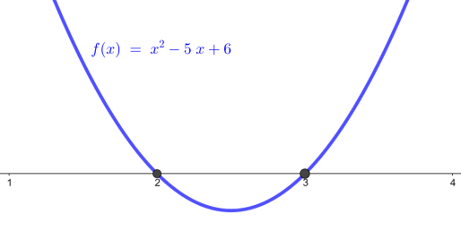
\includegraphics[width=\textwidth]{../Mathematik_1/Bilder/ungleichungen_quadratische_funktion_nullstellen.png}
\end{minipage}
\begin{minipage}{0.55\textwidth}
\begin{itemize}
\item Gezeigt ist der Graph der Funktion
\(
	f(x)=x^2-5x+6.
	\)
\item Positive Funktionswerte treten links der kleineren und rechts der gr��eren Nullstelle auf. Genau diese Bereiche bilden die zuvor berechnete L�sungsmenge.
\end{itemize}
\end{minipage}
\end{exabox}

\noindent\textbf{Bemerkungen:}
\begin{itemize}
\item Die L�sungsmenge l�sst sich damit sowohl rechnerisch als auch am Graphen erkennen.
\item Quadratische Terme lassen sich mithilfe ihrer Nullstellen faktorisieren:
\(
	ax^2+bx+c=a(x-x_1)(x-x_2).
	\)
\item Das Grundprinzip aus Nullstellenbestimmung und Vorzeichenanalyse bleibt auch bei polynomialen Ungleichungen h�herer Ordnung erhalten.
\end{itemize}

Bei einer \textbf{Bruchungleichung} kommt eine weitere Schwierigkeit hinzu: Das Vorzeichen eines Bruches h�ngt sowohl vom Z�hler als auch vom Nenner ab. Gleichzeitig darf der Nenner niemals Null werden. Eine Multiplikation mit dem Nenner ist deshalb erst dann m�glich, wenn bekannt ist, welches Vorzeichen dieser besitzt.

Besonders einfach ist der Fall, dass der Bruch mit Null verglichen wird. Ein Bruch ist nichtnegativ, wenn Z�hler und Nenner dasselbe Vorzeichen besitzen oder der Z�hler Null ist.

\begin{exabox}{L�sen einer Bruchungleichung mit rechter Seite Null}{ }
Betrachtet wird

$$
\frac{2x-1}{x+4}\geq0.
$$

Der Nenner darf nicht verschwinden, also gilt zun�chst

$$
x\neq-4.
$$

Damit der Bruch nichtnegativ ist, m�ssen Z�hler und Nenner gleiches Vorzeichen besitzen:

$$
\begin{array}{rcl}
\dfrac{2x-1}{x+4}\geq0
&\Leftrightarrow&
\begin{cases}
2x-1\geq0 \land x+4>0,\\
2x-1\leq0 \land x+4<0
\end{cases}
\\[2ex]
&\Leftrightarrow&
\begin{cases}
x\geq\dfrac12 \land x>-4,\\
x\leq\dfrac12 \land x<-4
\end{cases}
\\[2ex]
&\Leftrightarrow&
\begin{cases}
x\geq\dfrac12,\\
x<-4.
\end{cases}
\end{array}
$$

Die beiden F�lle werden vereinigt. Damit ergibt sich

$$
x\in(-\infty,-4)\cup\left[\frac12,\infty\right).
$$

\end{exabox}

Steht auf der rechten Seite dagegen eine von Null verschiedene Zahl, kann nicht allein das Vorzeichen des gesamten Bruches betrachtet werden. Um den Nenner zu beseitigen, m�sste mit \(x+4\) multipliziert werden. Dabei h�ngt die Richtung des Ungleichheitszeichens davon ab, ob \(x+4\) positiv oder negativ ist. Deshalb wird \textbf{zuerst das Vorzeichen des Nenners unterschieden}.

\begin{exabox}{L�sen einer Bruchungleichung mit konstanter rechter Seite}{ }
Betrachtet wird

$$
\frac{2x-1}{x+4}\geq3.
$$

Der Nenner verschwindet f�r \(x=-4\). Dieser Wert geh�rt nicht zum Definitionsbereich. F�r alle �brigen Werte werden zwei F�lle unterschieden.

$$
\begin{array}{rcll}
\dfrac{2x-1}{x+4}\geq3
&\Leftrightarrow&
\begin{cases}
x+4>0 \land 2x-1\geq3(x+4),\\
x+4<0 \land 2x-1\leq3(x+4)
\end{cases}
& \text{Nenner-Vorzeichen}
\\[3ex]
&\Leftrightarrow&
\begin{cases}
x>-4 \land x\leq-13,\\
x<-4 \land x\geq-13
\end{cases}
& \text{Ungleichungen l�sen}
\\[3ex]
&\Leftrightarrow&
\begin{cases}
x\in\emptyset,\\
x\in[-13,-4)
\end{cases}
& \text{F�lle auswerten}
\\[3ex]
&\Leftrightarrow&
x\in[-13,-4).
& \text{vereinigen}
\end{array}
$$

Im ersten Fall widersprechen sich die Bedingungen \(x>-4\) und \(x\leq-13\); dieser Fall liefert daher keine L�sung. Im zweiten Fall m�ssen \(x<-4\) und \(x\geq-13\) gleichzeitig erf�llt sein. Daraus entsteht das Intervall \([-13,-4)\).
\end{exabox}

Bei einer \textbf{Betragsungleichung} entsteht die Fallunterscheidung aus der Definition des Betrags. Der Betrag eines Ausdrucks h�ngt davon ab, ob dieser Ausdruck nichtnegativ oder negativ ist:

$$
|T|=
\begin{cases}
T,&T\geq0,\\
-T,&T<0.
\end{cases}
$$

F�r die Ungleichung \(|x-7|<5\) wird deshalb das Vorzeichen von \(x-7\) unterschieden.

\begin{exabox}{L�sen einer Betragsungleichung}{ }

$$
\begin{array}{rcl}
|x-7|<5
&\Leftrightarrow&
\begin{cases}
x-7\geq0 \land x-7<5,\\
x-7<0 \land -(x-7)<5
\end{cases}
\\[2ex]
&\Leftrightarrow&
\begin{cases}
x\geq7 \land x<12,\\
x<7 \land x>2
\end{cases}
\\[2ex]
&\Leftrightarrow&
\begin{cases}
x\in[7,12),\\
x\in(2,7)
\end{cases}
\\[2ex]
&\Leftrightarrow&
x\in(2,12).
\end{array}
$$

\end{exabox}

Bei einfachen Betragsungleichungen l�sst sich dasselbe Ergebnis auch unmittelbar aus der Bedeutung des Betrags ablesen:

$$
|x-7|<5
\;\Leftrightarrow\;
-5<x-7<5
\;\Leftrightarrow\;
2<x<12.
$$

Die ausf�hrliche Fallunterscheidung bleibt dennoch wichtig, da sie auch dann funktioniert, wenn kompliziertere Ausdr�cke innerhalb des Betrags auftreten.

Treten mehrere dieser Strukturen gleichzeitig auf, m�ssen die notwendigen Fallunterscheidungen miteinander kombiniert werden. Bei einem Betrag im Z�hler und einem variablen Nenner muss beispielsweise sowohl das Vorzeichen des Nenners als auch das Vorzeichen des Ausdrucks innerhalb des Betrags ber�cksichtigt werden.
 \newpage % �quivalenztransformationen 
\setcounter{exercise}{0} \ifintegriereaufgaben
\section*{�quivalenzumformungen Aufgaben}\label{MA1-aequivalenzumformungen-aufgaben}

Regeln und Beispiele, die zur Bearbeitung der Aufgaben hilfreich sind, finden Sie im Skript\wennreferenzvorhanden{MA1-aequivalenzumformungen}{ (Abschnitt \abschnittsverweis{MA1-aequivalenzumformungen})} und, falls Sie nicht weiterkommen, schauen Sie \hyperref[MA1-aequivalenzumformungen-loesungen]{hier}.

\else
\section{�quivalenzumformungen Aufgaben}\label{MA1-aequivalenzumformungen-aufgaben}

Regeln und Beispiele, die zur Bearbeitung der Aufgaben hilfreich sind, finden Sie im Skript und, falls Sie nicht weiterkommen, schauen Sie \hyperref[MA1-aequivalenzumformungen-loesungen]{hier}. 

\fi 

\begin{theorembox}{Allgemeine L�sungsformel}{ }
	Zur L�sung von Gleichungen \(a\cdot x^2+b\cdot x+c=0\) mit \(a,b,c\in \mathbb R\) berechnet man die sogenannte Diskriminante \(D=b^2-4\cdot a \cdot c\). F�r \(D\geq 0\) besitzt die Gleichung zwei reelle L�sungen. Sie lauten
	\[ x_{1,2} = \frac{-b\pm \sqrt{b^2-4\cdot a \cdot c} }{2\cdot a}\,.\]
	Mit den L�sungen \(x_{1,2}\) kann die Linearfaktorzerlegung des quadratischen Terms \(a\cdot x^2+b\cdot x+c\) angegebenen werden: 
	\[ a\cdot x^2+b\cdot x+c = a\cdot (x-x_1)\cdot (x-x_2)\,.\]
\end{theorembox}

\begin{exercisebox}[Gleichungen und Ungleichungen]
	Bestimmen Sie die L�sungsmengen der folgenden Gleichungen und Ungleichungen:
	\begin{eqnarray*}
	\begin{array}{ll}
		(a)\; \displaystyle{\frac{x+52}{x+2}} = 11  & \quad \quad (b)\; \displaystyle{\frac{x^2+2\cdot x-3}{x+3} = 1} \\[2ex] 
		(c)\; \displaystyle{\frac{(n+2)!}{n!}} = 72, n\in\mathbb N_0 &\quad\quad (d)\; \displaystyle{|2\cdot x-6|} = |4-5\cdot x|  \\[1ex] 
		(e)\; 3\cdot x-3 < 7 -2\cdot x & \quad\quad (f)\; \displaystyle{\frac{3\cdot x-5}{x-2}} \leq 3 \\[2ex] 
		(g)\; |6\cdot x+1|<|2\cdot x-1| &\quad\quad  (h)\; \displaystyle{\Big|\frac{3\cdot x+2}{x-2} \Big|} < 1 
	\end{array}
	\end{eqnarray*}
\end{exercisebox}

\begin{exercisebox}[Gleichungssystem]
	Bestimmen Sie jeweils die L�sungsmenge der folgenden Gleichungssysteme
		\begin{eqnarray*}
			\begin{array}{lll}
			
				(a)\; \begin{cases} 
		2\cdot y-4\cdot x &= -6 \\
		5\cdot y-4\cdot x &= -21
	\end{cases} &\quad  
	(b)\;\begin{cases}
		2\cdot x+y &= 7 \\
		2\cdot x+y &= 7
	\end{cases}  & \quad 
	(c)\;	\begin{cases}
		x^2+y^2 &= 10 \\
		x+y &= 4
	\end{cases}
\end{array}
\end{eqnarray*}
\end{exercisebox}

\begin{exercisebox}[Gleichungssystem mit Parameter]
	L�sen Sie das folgende lineare Gleichungssystem f�r \(p\in \mathbb R\)
		\begin{eqnarray*}
			\begin{array}{rcrcr}
		x_1 &+& p\cdot  x_2 &=& 1 \\
		(p-1)\cdot x_1 &+& x_2 &=& -1
	\end{array}
	\end{eqnarray*}
\end{exercisebox}

\begin{exercisebox}[Brainteaser]
	In einer Familie hat jeder Sohn gleich viele Schwestern und Br�der. Jede Tochter hat aber doppelt so viele Br�der wie Schwestern. Wie viele S�hne und T�chter hat die Familie?
\end{exercisebox}

\begin{exercisebox}[Brainteaser]
	Zu einem Fest auf dem Land fahren mehrere Pferdewagen mit der jeweils gleichen Anzahl an Personen. Auf halbem Weg fallen zehn Wagen aus, sodass jeder der �brigen Wagen eine weitere Person aufnehmen muss. Vor Antritt des R�ckwegs fallen weitere \(15\) Wagen aus, was zur Folge hat, dass in jedem Wagen drei Personen mehr sind als bei der Abfahrt am Morgen. Wie viele Personen nahmen an dem Fest teil?
\end{exercisebox}
 \newpage 
\setcounter{satz}{0} \setcounter{def}{0} \setcounter{exa}{0}  \section{Funktionen}\label{MA1-funktionen}

\begin{table}[H]
  \centering
  \begin{tabularx}{\textwidth}{p{0.9\textwidth} p{0.1\textwidth}}
    \toprule
	  \multicolumn{2}{c}{\textbf{�bersicht �ber Lernziele und Voraussetzungen}}\\
    \midrule
	  \textbf{Lernziele} &\\[.5\normalbaselineskip]
\tabitem Funktionen als eindeutige Zuordnungen pr�zise beschreiben &\\
\tabitem Definitionsbereich, Zielmenge und Bildmenge unterscheiden und bestimmen &\\
\tabitem Funktionen in mathematischer Formelsprache darstellen und interpretieren &\\
\tabitem Funktionsgraphen als Mengen geordneter Paare interpretieren &\\
\tabitem Funktionen von allgemeineren Relationen unterscheiden &\\
    \midrule
	  \textbf{Voraussetzungen} \\[.5\normalbaselineskip]
	  \tabitem Mengenoperationen und Intervallschreibweisen & \abschnittsverweis{MA1-mengen-und-logik}\\
	  \tabitem Grundrechenarten & \abschnittsverweis{MA1-zahlenmengen}\\
	  \tabitem �quivalenzumformungen & \abschnittsverweis{MA1-aequivalenzumformungen}\\
    \bottomrule
  \end{tabularx}
\end{table}

\ifintegriereaufgaben \noindent �bungsaufgaben zum Thema finden Sie hier: \hyperref[MA1-funktionen-aufgaben]{Aufgaben}
\vspace{0.3cm}
\hrule
\fi

\subsection{Was ist eine Funktion?}

Eine \textbf{Abbildung} (\emph{mapping}) namens $f$ ordnet jedem Element $x$ eines Definitionsbereichs $D$ (\emph{domain}) genau ein Element $y$ einer Zielmenge  $Z$ (\emph{codomain}) zu. In mathematischer Kurzschreibweise sieht das so aus:
	\[ f: D \to Z, x\mapsto y\,.\]
	Dieser Ausdruck sagt aber noch nichts dar�ber, wie die Abbildung im Detail funktioniert. Was fehlt ist die Zuordnungsvorschrift oder Abbildungsvorschrift. Anstatt eine "\,Gleichung $y=f(x)$"\, wie in der Schule anzugeben, f�hren wir einen Abbildungspfeil ein: 
	\[  x\mapsto f(x)\,.\]
	Da der Definitionsbereich, die Zielmenge und die Abbildungsvorschrift zusammen eine Abbildung so definieren, dass man in der Lage ist die Abbildung zu untersuchen, fasst man diese Informationen typischerweise zusammen und gibt eine Abbildung in der folgenden Form an:  
\begin{defbox}{Abbildung von \(D\) nach \(Z\) mit Abbildungsvorschrift}{ }
	$ f: D\to Z, x\mapsto f(x)\,.$
\end{defbox}
\noindent{\textbf{ Bemerkungen:}}
\begin{itemize}
	\item Statt $f(x)$ wird typischerweise eine Formel angegeben, beispielsweise $ x\mapsto \sin(x)$ oder \( x\mapsto 10\cdot x^3-2\cdot\sqrt{x}\).
	\item Wenn der Definitionsbereich und die Zielmenge fixierte Mengen von Zahlen, von geometrischen Objekten oder von Funktionen (!) \dots  sind, nennt man eine Abbildung meist eine Funktion (\emph{function}). Mathematisch sind Abbildungen und Funktionen dasselbe. 
\end{itemize}

Es gibt mehrere Vorstellungen von Abbildungen (Funktionen). Hier sind vier davon. 

\begin{exabox}{Funktion als Maschine}{ }
\begin{minipage}{0.3\textwidth}
	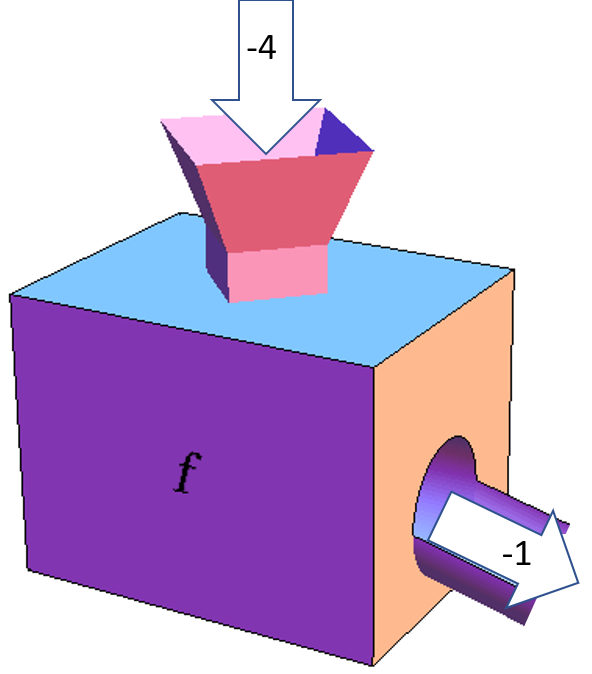
\includegraphics[width=\textwidth]{../Mathematik_1/Bilder/funktionen_maschinenmodell_zahlenwerte.png} 
\end{minipage}
\begin{minipage}{0.7\textwidth}
Eine Abbildung $f$ ist eine Maschine, in die man ein Teil aus einer Menge $D$ als Rohmaterial hineinwerfen kann und aus der man dann ein Teil aus $Z$ als Produkt zur�ckerh�lt:
\begin{itemize}
	\item Alle Teile aus $D$ m�ssen akzeptiert werden.
	\item Nur Teile aus $Z$ d�rfen produziert werden. 
	\item Es wird immer genau ein Teil produziert (nicht null, nicht sieben). 
	\item Wenn man dasselbe Teil aus $D$ nochmal hinein wirft, muss wieder dasselbe Teil aus $Z$ produziert werden wie beim ersten Mal. 
\end{itemize}
\end{minipage}
\end{exabox}

\begin{exabox}{Funktion als Tabelle}{ }
\begin{minipage}{0.2\textwidth}
	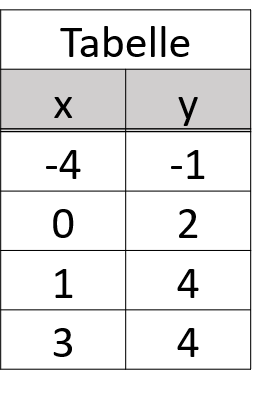
\includegraphics[width=\textwidth]{../Mathematik_1/Bilder/funktionen_darstellung_wertetabelle.png} 
\end{minipage}
\begin{minipage}{0.7\textwidth}
Eine Abbildung $f$ ist eine Tabelle (ggf unendlich lang), aus der man f�r jedes $x\in D$ das zugeh�rige $f(x) \in Z$ ablesen kann:
\begin{itemize}
	\item In der $x$-Spalte der Tabelle muss jedes Element aus $D$ genau einmal vorkommen (nicht null mal, nicht sieben mal). 
	\item In der $y$-Spalte der Tabelle d�rfen nur Elemente aus $Z$ stehen. 
	\item In dem Beispiel ist $Z=\mathbb Z$. 
	\item Die Reihenfolge der Zeilen in der Tabelle ist egal. 
\end{itemize}
\end{minipage}
\end{exabox}

\begin{exabox}{Funktion als Pfeildiagramm}{ }
\begin{minipage}{0.3\textwidth}
	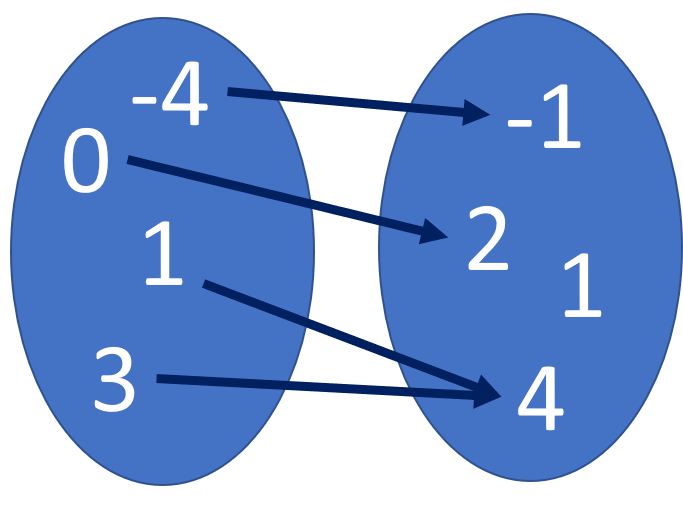
\includegraphics[width=\textwidth]{../Mathematik_1/Bilder/funktionen_darstellung_pfeildiagramm.png} 
\end{minipage}
\begin{minipage}{0.7\textwidth}
\begin{itemize}
	\item Von jedem Element in $D$ muss genau ein Pfeil starten und zu einem Element in $Z$ f�hren. 
	\item Es ist erlaubt, dass mehrere Pfeile auf einem Element von $Z$ enden. 
	\item Es ist auch erlaubt, dass Elemente von $Z$ von keinem Pfeil erreicht werden. 
\end{itemize}
\end{minipage}
\end{exabox}

\begin{exabox}{Funktion als Graph}{ }
\begin{minipage}{0.3\textwidth}
	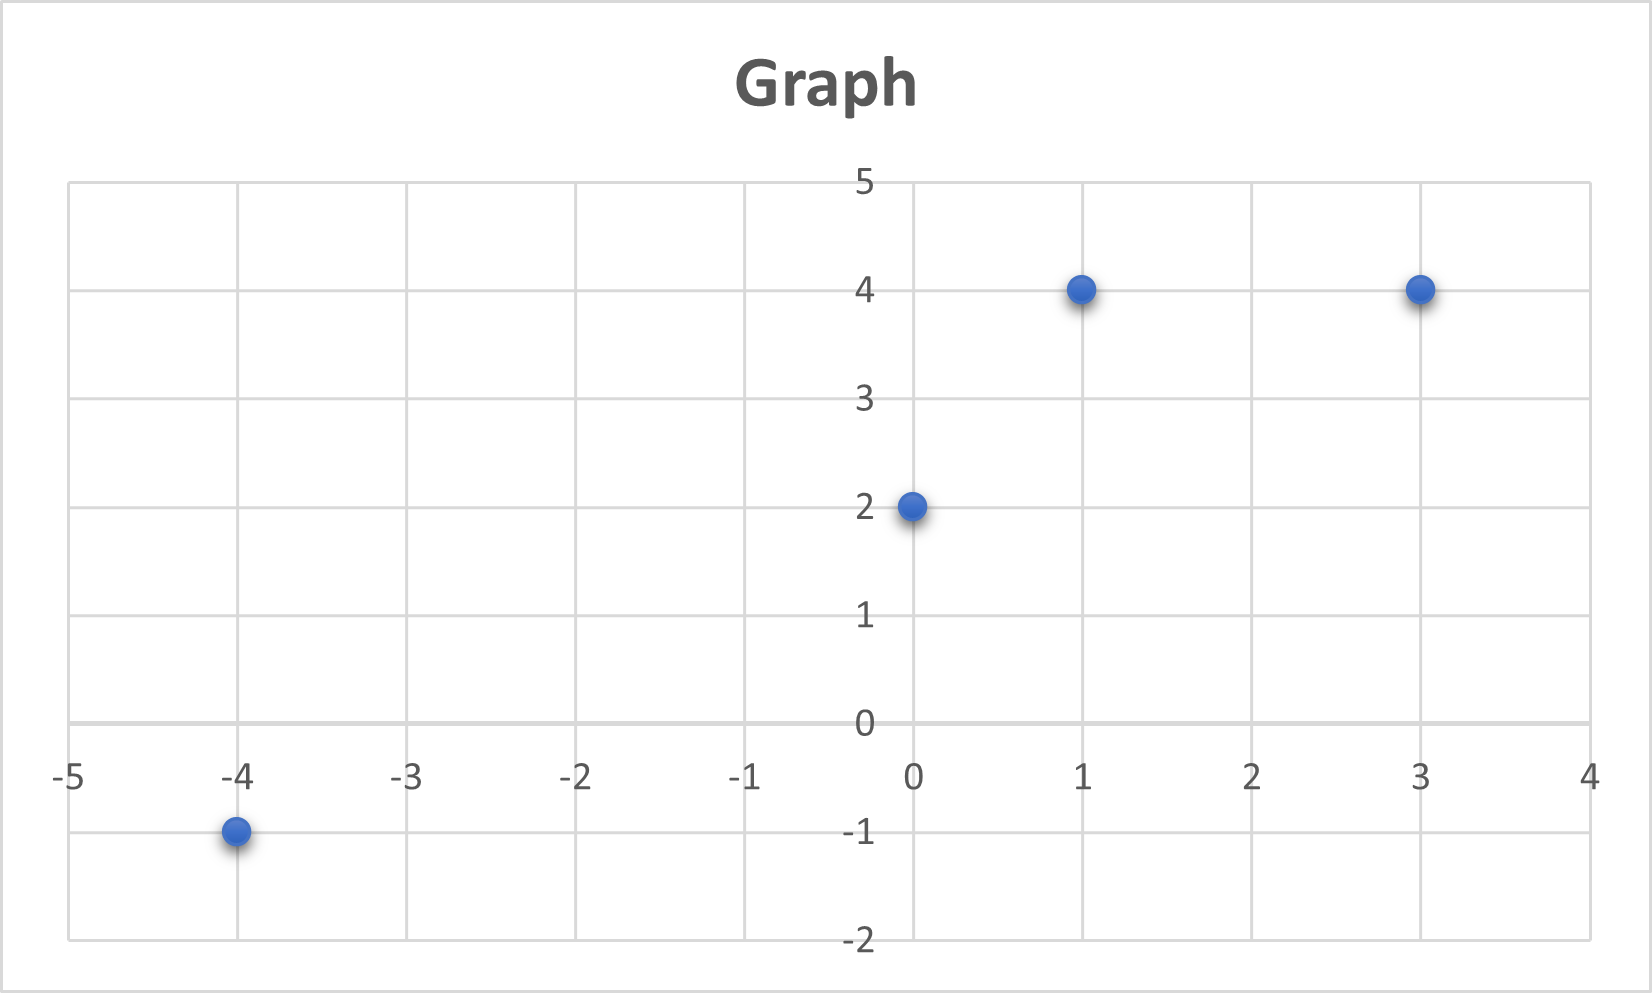
\includegraphics[width=\textwidth]{../Mathematik_1/Bilder/funktionen_darstellung_diskreter_graph.png} 
\end{minipage}
\begin{minipage}{0.7\textwidth}
 Hier ist von Funktionen die Rede, die man in einem Diagramm aufmalen kann. 
\begin{itemize}
	 \item $D$ und $Z$ sind also Mengen von Zahlen. 
	 \item Der Definitionsbereich \(D\) wird auf der \(x\)-Achse dargestellt, die Zielmenge \(Z\) auf der \(y\)-Achse.
	 \item $D$ und $Z$ k�nnen sich nat�rlich auch jeweils �ber die gesamten Achsen erstrecken. 
	 \item Zu jedem $x\in D$ (und nur f�r solche $x$ ) ist genau ein $y\in Z$ markiert. 
 \end{itemize}
\end{minipage}
\end{exabox}

  
\subsection{Definitions- und Bildbereich}

Der \textbf{Definitionsbereich} ist die Menge aller mathematischen Objekte, die in eine Funktion hineingegeben werden d�rfen. In der Pfeilvorstellung einer Funktion bildet der Definitionsbereich den Startpunkt der Pfeile; die Pfeilspitzen liegen in der \textbf{Zielmenge}. 

Diese Vorstellung findet sich unmittelbar in der mathematischen Schreibweise

$$
f:D\to Z,\qquad x\mapsto f(x)
$$

wieder: Ein Element \(x\in D\) am Pfeilanfang wird auf ein Element \(f(x)\in Z\) an der Pfeilspitze abgebildet.

Definitionsbereich \(D\) und Zielmenge \(Z\) sind h�ufig Teilmengen der reellen Zahlen -- oder sogar ganz \(\mathbb R\). Im folgenden Beispiel muss der Definitionsbereich $D \subsetneq \mathbb R$ eingeschr�nkt werden, weil die Funktion an der Stelle $x=3$ nicht definiert ist:\marginpar{Aufgabe}
\begin{exabox}{Funktion mit $D \subsetneq \mathbb R$}{ }
  $f: D \to \mathbb R, \; x\mapsto \displaystyle{\frac{x^2+7}{x-3}} \Rightarrow D = \mathbb R\setminus \{3\}\,.$
\end{exabox}

Hinter den meisten �blichen Operationen mit Zahlen stecken Funktionen - auch wenn sie oft nicht explizit als solche bezeichnet werden: 
\begin{itemize}
  \item Addition reeller Zahlen: $ +:\, \mathbb R^2 \to \mathbb R,\; (x,y) \mapsto x+y\,,$ 
  \item Division reeller Zahlen: $ /:\, \{(x,y)\in \mathbb R^2: y \not = 0\} \to \mathbb R,\; (x,y) \mapsto \displaystyle{\frac{x}{y}}\,,$
  \item Fakult�t: $!:\, \mathbb N_0 \to \mathbb N^+,\; n \mapsto n\cdot(n-1)\cdot(n-2)\cdot \dots \cdot 2\cdot 1 =: n!\,,$ 
  \item Binomialkoeffizient: $ \displaystyle{{\cdot}\choose{\cdot}}:\, \big\{ (n,k)\in\mathbb N_0^2: k\leq n\big\} \to \mathbb N_0,\; (n,k) \mapsto \displaystyle{ \frac{n!}{k!\cdot (n-k)!} }\,.$ 
\end{itemize}


 
Die Menge der tats�chlich angenommenen Funktionswerte hei�t \textbf{Bild}, \textbf{Bildbereich} oder \textbf{Bildmenge}\marginpar{\small{Aufgabe}} (\emph{image}) und wird mit \(f(D)\) bezeichnet. Dabei gilt

$$
f(D)\subseteq Z.
$$

Die Bildmenge kann also kleiner als die Zielmenge sein, sie kann aber auch mit der Zielmenge �bereinstimmen.

Die Menge $S$, die in einem der folgenden Beispiele auftaucht, bezeichne die Menge aller endlichen Zeichenketten.

\begin{exabox}{Unterschiedliche Bildmengen}{ }
\begin{itemize}
  \item $f_1: [3,4] \to \mathbb R,\; x\mapsto x^2 \; \Rightarrow \; f_1(D) = [9,16]$. 

\item   $f_2:S \to S, \; x\mapsto \displaystyle{\begin{cases} \verb-a-, \quad x=\verb-b- \\  x, \quad x\not=\verb-b- \end{cases}} \Rightarrow \; f_2(D) = S\setminus \{ \verb-b-\}$.

\item $f_3: \mathbb R \to \mathbb R^2,\; t \mapsto \left(\cos(2\pi t), \sin(2\pi t)\right) \; \Rightarrow \; f_3(D) = \left\{(x,y)\in \mathbb R^2:  x^2 + y^2 = 1\right\}\,.$

\item $f_4: \mathbb R \to \mathbb R^2,\; t\mapsto \left(e^t \cdot \cos(2 \pi\cdot t), e^t \cdot \sin(2 \pi\cdot t)\right)$ Die Bildmenge bildet geometrisch eine logarithmische Spirale.  \end{itemize}
\end{exabox}

Die folgende Skizze veranschaulicht den Definitionsbereich $D$, die Zielmenge $Z$ und die Bildmenge $f(D)$ einer Funktion $f$.

\begin{center}
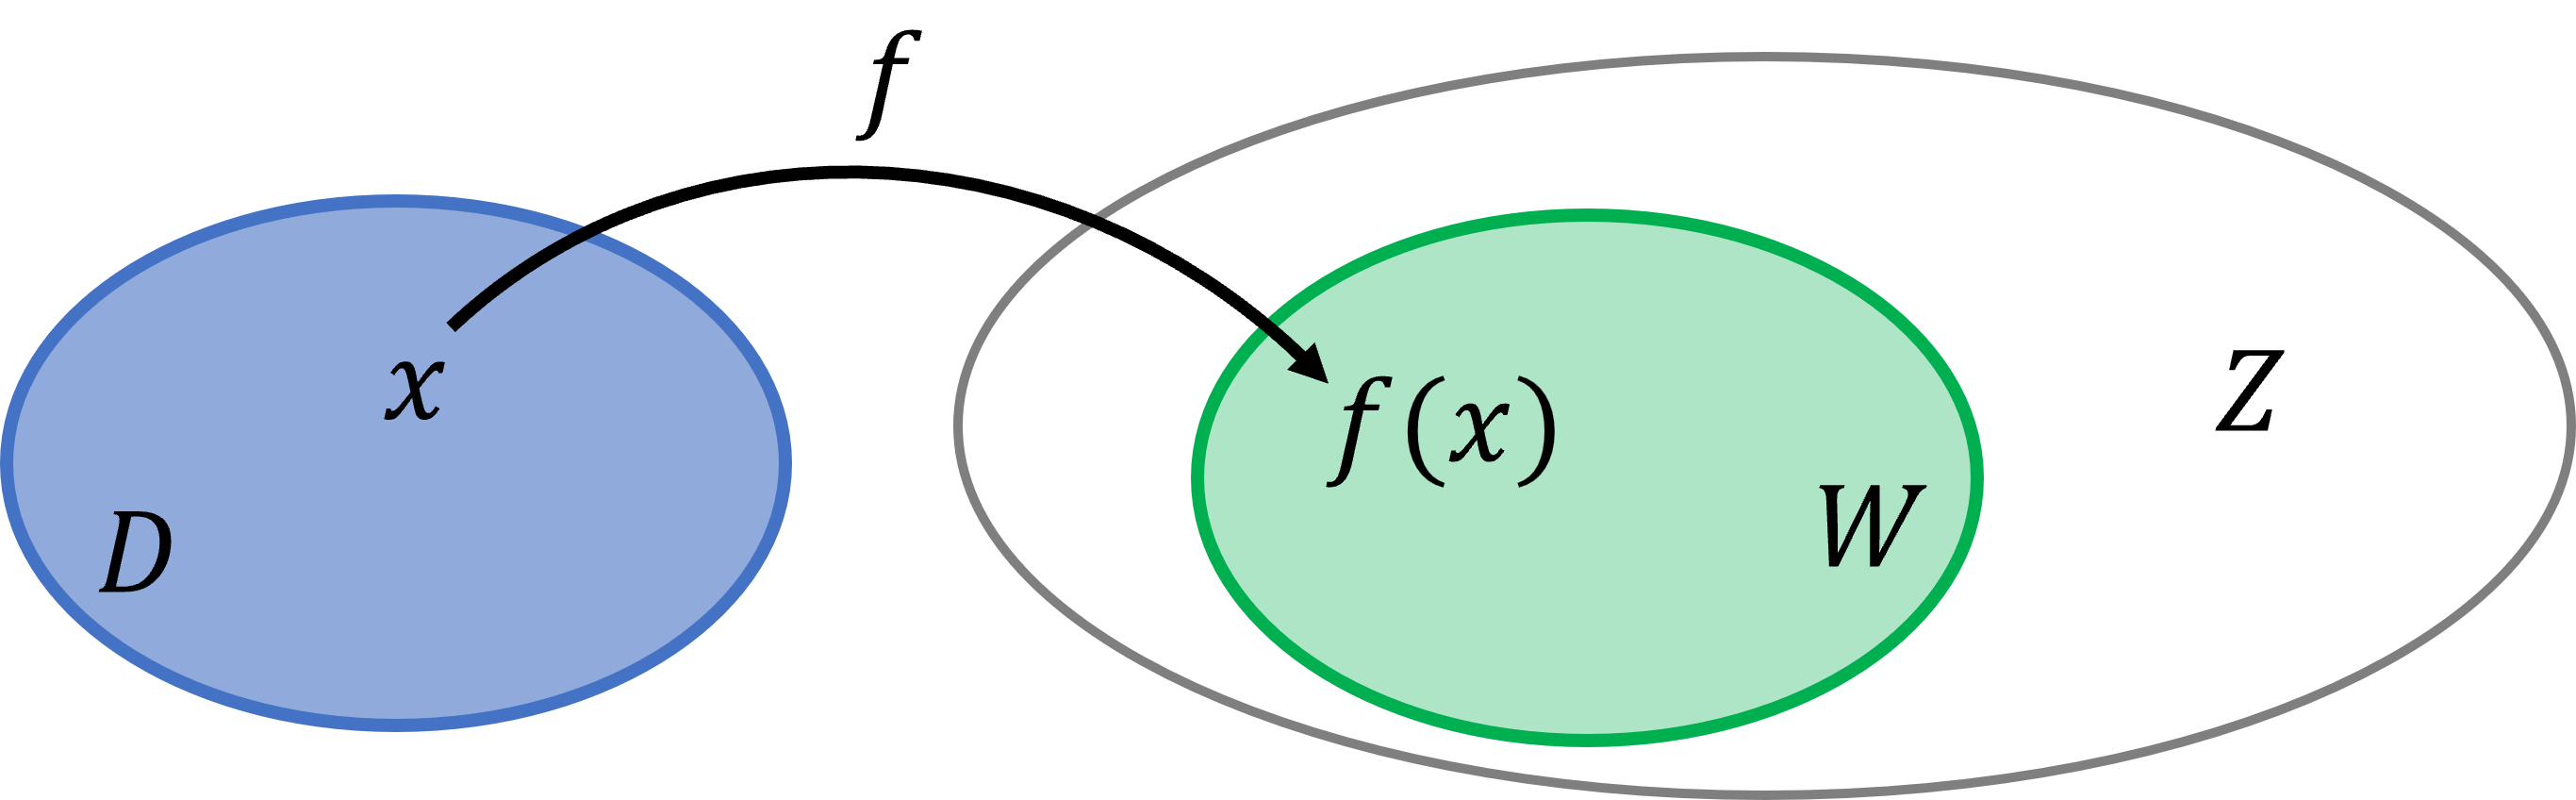
\includegraphics[width=0.8\textwidth]{../Mathematik_1/Bilder/funktionen_definitionsbereich_zielmenge_bildmenge.png}
\end{center}

\noindent{\textbf{ Bemerkungen:}}
\begin{itemize}
	\item Der Name der Funktion ist $f$. Der Ausdruck $f(x)$ bezeichnet den Funktionswert von \(f\) an der Stelle \(x\) und ist ein Element der Zielmenge $Z$. 
	\item Fiese (pathologische) Funktionen bilden keine anschaulichen Graphen. Die Dirichlet Funktion ist eine von ihnen: 
  $$ f: \mathbb R \to \{0, 1\}, \quad x\mapsto \begin{cases} 1,\quad x\in \mathbb Q, \\ 0,\quad x\in \mathbb R\setminus{\mathbb Q}\,.\end{cases} $$
  \item Eine Funktion braucht nicht unbedingt eine ausdr�ckliche Abbildungsvorschrift wie $x \mapsto \sin(x^{2})$ zu haben. Eine Abbildung kann auch in Worten beschrieben werden, beispielsweise
	  \begin{center}
  "Nimm den dritten Buchstaben von $x$, falls vorhanden, ansonsten $*$." 
  \end{center}
  Oder sie ist nur indirekt gegeben, zum Beispiel als Stammfunktion:
  \begin{center}
  "$F$ ist die Stammfunktion von $x\mapsto e^{-x}$ f�r $F(0)=0$."
  \end{center}
\item Beim Programmieren kommen ebenfalls sogenannte Funktionen vor. Der Funktionsbegriff in Programmiersprachen ist jedoch allgemeiner als der mathematische Funktionsbegriff; beispielsweise k�nnen Programmfunktionen ohne explizite Eingabe aufgerufen werden.	
\end{itemize}

\subsection{Funktionsgraphen und Relationen}

F�r eine Funktion

$$
f:D\to Z
$$

kann jede Zuordnung \(x\mapsto f(x)\) als geordnetes Paar

$$
(x,f(x))\in D\times Z
$$

aufgefasst werden. Der \textbf{Graph einer Funktion} ist die Menge all dieser Paare:

$$
G_f
=
\{(x,f(x)):x\in D\}
\subseteq D\times Z.
$$

Die formale Schreibweise f�r den Graphen $G_f$ bedeutet: F�r jedes \(x\) aus dem Definitionsbereich wird das geordnete Paar aus \(x\) und dem zugeh�rigen Funktionswert \(f(x)\) in den Graphen aufgenommen.

F�r eine reelle Funktion \(f:D\to\mathbb R\) mit \(D\subseteq\mathbb R\) gilt insbesondere

$$
G_f\subseteq\mathbb R^2.
$$

Deshalb l�sst sich der Funktionsgraph als Menge von Punkten in der Ebene darstellen.

Allerdings ist nicht jede Teilmenge von \(\mathbb R^2\) der Graph einer Funktion. Die Kreislinie liefert daf�r ein anschauliches Beispiel.

%\subsection{Geordnete Tupel}
%
%Wenn man ein Gef�hl f�r den Funktionsverlauf einer Funktion \(f: \mathbb R \to \mathbb R,\, x\mapsto f(x)\) bekommen m�chte, dann geht man oft wie folgt vor 
%\begin{enumerate}
%	\item man w�hlt eine paar Werte f�r \(x \in \mathbb R\): das sind die St�tzstellen \(x_i, \, i=1,2,3,\cdots\)
%	\item man berechnet die zu den St�tzstellen geh�rigen Funktionswerte \(y_i = f(x_i) \in \mathbb R\)
%	\item man zeichnet in ein zwei-dimensionales Koordinatensystem die Punkte \(P_i = (x_i|y_i)\) 
%	\item man verbindet die Punkte miteinander und behauptet, dass die Funktion so aussieht!\footnote{Falls die Funktion stetig ist, ist das ein guter Ansatz!}
%\end{enumerate} 
%
%Die Punkte \(P(x|y)\), die zu \(f\) geh�ren sind Tupel und das hei�t, dass die Reihenfolge der Koordinaten fixiert ist und eine Rolle spielt: erst \(x\) dann \(y\). 

\begin{exabox}{Funktionsgraph oder nicht?}{ }
\begin{minipage}{0.3\textwidth}
	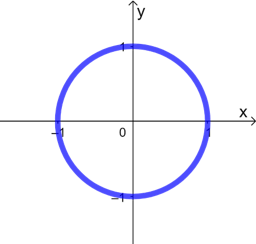
\includegraphics[width=\textwidth]{../Mathematik_1/Bilder/relationen_einheitskreis.png} 
\end{minipage}
\begin{minipage}{0.7\textwidth}
\begin{itemize}
	\item Ist die Kreislinie der Graph einer Funktion? 
	\item Wie l��t sich die Kreislinie beschreiben? 
\end{itemize}
\end{minipage}
\end{exabox}

Die Figur links, die Kreislinie, ist nicht der Graph einer Funktion, denn zu fast jedem \(x \in (-1,1) \) m�ssten zwei verschiedene Funktionswerte zugeordnet werden!\footnote{Die Kreislinie ist eine sogenannte Relation. Eine Relation ist etwas allgemeineres als eine Funktion.}

\subsection{Was ist eine Relation?}

Eine \textbf{Relation} beschreibt, welche Elemente mehrerer Mengen miteinander in Beziehung stehen. Formal ist eine beliebige Teilmenge eines \underline{kartesischen Produkts}\randverweis{MA1-mengen-und-logik}

$$
A_1\times A_2\times\cdots\times A_n
$$

eine \textbf{\(n\)-stellige Relation}.

Eine zweistellige Relation besteht damit aus geordneten Paaren, eine dreistellige Relation aus geordneten Tripeln usw.

\begin{exabox}{Relationen}{ }
  \begin{itemize}
    \item $\{ (1,2), (3,4), (1,5)\} \subseteq \mathbb N_0 \times \mathbb N_0$ 
    \item $\left\{ \left(\mathrm{Anton}, \mathrm{Weber}, 293\right), \left(\mathrm{Bea}, \mathrm{Knorr}, 298\right), \left(\mathrm{Lisa}, \mathrm{Kann}, 284\right) \right\} \subseteq S\times S\times \mathbb N_0$
  \end{itemize}
\end{exabox}

Das zweite Beispiel l�sst die wesentliche Bedeutung von Relationen in der Informatik erahnen: sie dienen als Datenspeicher.

Es gibt mehrere �bliche Vorstellungen von Relationen. Hier sind drei davon. 

\begin{enumerate}
  \item {\textbf{Tabelle:}} Fast alle aktuell �blichen  Datenbanksysteme verwalten Tabellen. Mathematische Relationen sind nichts anderes als Tabellen mit  ein  paar  Besonderheiten.  Deshalb  hei�en  diese  Datenbanksysteme auch relational.

\begin{center}
  \begin{tabular}{c|c|c}
    Vorname & Nachname & Matrikelnummer \\
    \hline
  Bea & Knorr & $298$ \\
  Lisa & Kann & $284$ \\
  Anton & Weber & $293$
  \end{tabular}
\end{center}

\begin{itemize}
  \item In jeder Spalte der Tabelle d�rfen nur Eintr�ge aus der jeweiligen Menge des kartesischen Produkts stehen. 
  \item Die Reihenfolge der Zeilen ist egal. 
  \item Keine Zeile darf als Ganzes doppelt vorkommen; Teile der Zeile d�rfen sich aber wiederholen. 
\end{itemize}
      
Bei Abbildungen bzw. Funktionen gibt es im Unterschied zur Relation nur zwei Spalten. Au�erdem \textbf{muss} in der linken Spalte jedes Elemente des Definitionsbereichs vorkommen - und das \textbf{genau einmal}. %Frage


\item {\textbf{Liniendiagramm:}}
  \begin{itemize}
    \item Elemente  der  Mengen  aus  dem  Produkt  sind  durch  Linien  verbunden.  
    \item Jede Linie geht durch genau ein Element aus jeder Menge des kartesischen Produkts. 
    \item Linien d�rfen teilweise �bereinander liegen. 
    \item Keine zwei beliebige Linien d�rfen aber komplett �bereinstimmen. 
  \end{itemize}

Bei Abbildungen bzw. Funktionen malt man typischerweise Pfeile statt Linien. Au�erdem sind nur zwei Mengen beteiligt und es muss von jedem Element des Definitionsbereichs genau ein Pfeil ausgehen. 


\item {\textbf{Geometrische Objekte im $\mathbb R^n$:}}

Eine $n$-stellige Relation zwischen reellen Zahlen ist eine Teilmenge des $\mathbb R^n$, also eine Menge von Punkten. Umgekehrt ist jedes auch noch so komische geometrische Objekt eine Relation! 

\begin{exabox}{Relationen}{ }
  \begin{itemize}
    \item die Kreislinie: $P:=\left\{ (x,y)\in \mathbb R^2: x^2+y^2 = 1\right\}$.
	  \item die �Gr��er-Gleich�-Relation: $\geq := \left\{ (x,y)\in \mathbb R^2: x\geq y \right\}$,
\end{itemize}
	\centering
	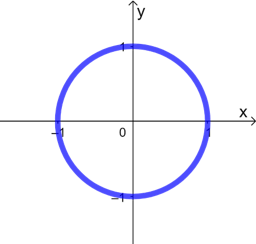
\includegraphics[width=0.4\textwidth]{../Mathematik_1/Bilder/relationen_einheitskreis.png} \hspace{2cm}
	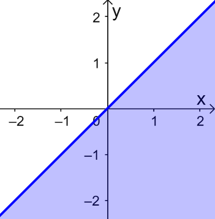
\includegraphics[width=0.4\textwidth]{../Mathematik_1/Bilder/relationen_halbebene_y_kleiner_gleich_x.png}
\end{exabox}

Bei einem Funktionsgraph muss jedem $x$ aus dem Definitionsbereich genau ein $y$ (nicht null, nicht zwei oder mehr) aus der Bildmenge zugeordnet werden, diese Einschr�nkung gilt nicht f�r Relationen.
\end{enumerate}


Eine Funktion ist damit eine besondere zweistellige Relation. F�r eine Funktion $ f:D\to Z $ muss zu jedem \(x\in D\) genau ein \(y\in Z\) geh�ren. Eine allgemeine Relation besitzt diese Einschr�nkung nicht: Zu einem \(x\) k�nnen kein, genau ein oder mehrere \(y\)-Werte geh�ren.

Der Funktionsgraph $ G_f=\{(x,f(x)):x\in D\} $ ist daher eine Relation mit einer zus�tzlichen Eindeutigkeitsbedingung.
 \newpage % Funktionen Grundlagen
\setcounter{exercise}{0} %%%% Pingo
%\begin{exercisebox}[Funktion - ja oder nein?]
%	Entscheiden Sie, ob die folgenden Skizzen Graphen einer Funktion \(f: X \to Y\) sein k�nnen. 
%	\centering
%	\includegraphics[width=0.9\textwidth]{../Mathematik_1/Bilder/Funktionen_ja_oder_nein.png}
%\end{exercisebox} 
%\begin{exercisebox}[Eigenschaften]
%	\begin{center}
%		\includegraphics[width=0.5\textwidth]{../Mathematik_1/Bilder/Rennstrecke.png}\hspace{1cm}
%	\includegraphics[width=0.3\textwidth]{../Mathematik_1/Bilder/Rennstrecken.png}
%	\end{center}
%  Der Graph zeigt, wie sich die Geschwindigkeit $\boldsymbol v$ eines Rennwagens w�hrend seiner zweiten Runde auf einer ebenen Rennstrecke ver�ndert.
%  \begin{enumerate}
%    \item Wie lang ist eine Runde?
%    \item Nennen Sie die niedrigste Geschwindigkeit und die h�chste Geschwindigkeit des Rennwagens.
%    \item Wie h�ufig musste der Rennfahrer abbremsen? Was k�nnten m�gliche Gr�nde sein?
%    \item Auf welcher Strecke war er unterwegs?
%\end{enumerate} 
%\end{exercisebox} 

\ifintegriereaufgaben
\section*{Funktionen Aufgaben}\label{MA1-funktionen-aufgaben}

Regeln und Beispiele, die zur Bearbeitung der Aufgaben hilfreich sind, finden Sie im Skript\wennreferenzvorhanden{MA1-funktionen}{ (Abschnitt \abschnittsverweis{MA1-funktionen})} und, falls Sie nicht weiterkommen, schauen Sie \hyperref[MA1-funktionen-loesungen]{hier}.

\else
\section{Funktionen Aufgaben}\label{MA1-funktionen-aufgaben}

Regeln und Beispiele, die zur Bearbeitung der Aufgaben hilfreich sind, finden Sie im Skript und, falls Sie nicht weiterkommen, schauen Sie \hyperref[MA1-funktionen-loesungen]{hier}. 
\fi 

\begin{exercisebox}[Funktionale Abh�ngigkeiten]
  Die Tabelle gibt den Verpackungsverbrauch pro Jahr von Privathaushalten und Kleinbetrieben in Millionen Tonnen an. 
  \begin{enumerate}
    \item Veranschaulichen Sie die Werte der Tabelle durch einen Graphen.
    \item Wann wurde vermutlich die neue Verpackungsverordnung (Gr�ner Punkt) eingef�hrt?
    \item Wie hoch w�re der Verpackungsverbrauch $1993$ wohl gewesen, wenn man die neue Verpackungsverordnung nicht eingef�hrt h�tte? Wie viel Prozent an Verpackungsmaterial wurde dadurch etwa eingespart?
  \end{enumerate}
  \begin{center}
  \begin{tabular}{c|c}
    Jahr & Verbrauch in Mio. Tonnen \\
    \hline
    $1988$ & $5.7$\\
    $1989$ & $6.4$\\
    $1990$ & $7.1$\\
    $1991$ & $7.6$\\
    $1992$ & $7.2$\\
    $1993$ & $7.0$\\
    $1994$ & $6.9$\\
    $1995$ & $6.7$
  \end{tabular}
  \end{center}
\end{exercisebox} 

\begin{exercisebox}[Mathematische Kurzschreibweise]
  Dr�cken Sie die Aussagen in mathematischer Kurzschreibweise aus.
  \begin{enumerate}
    \item Durch die Funktion $f$ wird der Zahl $3$ die Zahl $10$ zugeordnet.
    \item Die Funktion $g$ nimmt an der Stelle $5$ den Funktionswert $12$ an.
    \item Die Zahl $3$ geh�rt nicht zur Definitionsmenge der Funktion $f$.
    \item Die Funktion $f$ ordnet der Zahl $4$ einen gr��eren Funktionswert zu als der Zahl $5$.
    \item Die Funktionen $f$ und $g$ nehmen f�r $x=2$ denselben Funktionswert an.
    \item Alle Funktionswerte der Funktion $g$ sind positiv.
  \end{enumerate}
\end{exercisebox}

\begin{exercisebox}[Definitionsbereich]
	Bestimmen Sie den maximalen Definitionsbereich der folgenden Abbildungen:
  \begin{eqnarray*}
	  \begin{array}{lll}
		  (a) \; x\mapsto (x-1)^2 &\quad \quad (b)\; x\mapsto 3-5\cdot x-x^2 & \quad \quad (c)\; x\mapsto \displaystyle{\frac{1}{x}} \\[2ex]
		  (d) \; x\mapsto \displaystyle{\frac{1}{3-x}} & \quad \quad (e)\; x\mapsto \displaystyle{\frac{1}{(x-1)^2}} &\quad \quad (f) \; x\mapsto \displaystyle{\frac{1}{x^2-1}} \\[2ex]
		  (g) \; x\mapsto \sqrt{x-3} &\quad \quad (h) \; x\mapsto \displaystyle{\frac{1}{\sqrt{x-3}}} &\quad \quad (i)\; x\mapsto \ln( x +3) 
	  \end{array}
  \end{eqnarray*}
\end{exercisebox}

\begin{exercisebox}[Bildbereich]
	Bestimmen Sie den Bildbereich (die Bildmenge) der folgenden Abbildungen:
  \begin{eqnarray*}
	  \begin{array}{lll}
		  (a)\; x\mapsto x^2 & \quad \quad (b)\; x\mapsto x^2 +1 & \quad \quad (c)\; x\mapsto 2 - x^2 \\[2ex]
		  (d)\; x\mapsto -(x+2)^2+3 &\quad \quad (e)\; x\mapsto 3\cdot x-0.5 &\quad\quad (f)\; x\mapsto \sin( x) \\[2ex]
    (g)\; x\mapsto 3^x &\quad \quad (h)\; x\mapsto 3 
    \end{array}
  \end{eqnarray*}
\end{exercisebox}

%\begin{exercisebox}[Graphen lesen, Maxima, Minima, Symmetrie]
%	\begin{center}
%	\includegraphics[width=0.4\textwidth]{../Mathematik_1/Bilder/Mountainbike.png}
%	\end{center}
%  Eine Mountainbike Tour in dem spanischen El-Ports-Gebirge hat das abgebildete H�henprofil. 
%  \begin{enumerate}
%    \item Wie viele H�henmeter sind beim ersten Anstieg zu �berwinden?
%    \item Wie gro� ist der Gesamtanstieg, der bei der Tour zu �berwinden ist?
%    \item Wie steil ist die letzte Abfahrt ab Streckenkilometer $26$? Geben Sie das Gef�lle in Prozent und den Steigungswinkel an.
%    \item Zur Quelle Canaleta f�hrt nur eine Sackgasse. Wie �u�ert sich das im Graphen? Wie lang ist vermutliche diese Sackgasse?
%    \item Wo kann es noch eine Weitere Sackgasse geben?
%  \end{enumerate}
%
%%  \begin{tabular}{c|c}
%%    Kilometer & H�henmeter \\
%%    $0$ & $550$\\
%%    $1$ & $700$\\
%%    $4$ & $800$\\
%%    $5$ & $630$\\
%%    $6$ & $\ldots$
%%  \end{tabular}
%\end{exercisebox} 
 \newpage 
\setcounter{satz}{0} \setcounter{def}{0} \setcounter{exa}{0}  \section{Eigenschaften von Funktionen}\label{MA1-eigenschaften-von-funktionen}

\begin{table}[H]
  \centering
  \begin{tabularx}{\textwidth}{p{0.9\textwidth} p{0.1\textwidth}}
    \toprule
	  \multicolumn{2}{c}{\textbf{�bersicht �ber Lernziele und Voraussetzungen}}\\
    \midrule
	  \textbf{Lernziele} &\\[.5\normalbaselineskip]
    \tabitem Nullstellen einer Funktion bestimmen &\\
    \tabitem das asymptotische Verhalten einer Funktion qualitativ angeben &\\
    \tabitem Monotonie und Symmetrie pr�fen &\\
    \tabitem Periodizit�t pr�fen &\\
    \tabitem Injektivit�t, Surjektivit�t und Bijektivit�t unterscheiden &\\
    \tabitem die Umkehrbarkeit einer Funktion bestimmen &\\
    \tabitem die genannten Eigenschaften zur Erstellung eines Funktionsgraphen einsetzen &\\[.5\normalbaselineskip]
    \midrule
	  \textbf{Voraussetzungen} \\[.5\normalbaselineskip]
	  \tabitem Grundrechenarten & \abschnittsverweis{MA1-zahlenmengen}\\
	  \tabitem �quivalenzumformungen & \abschnittsverweis{MA1-aequivalenzumformungen}\\
	  \tabitem Definition einer Funktion & \abschnittsverweis{MA1-funktionen}\\
    \bottomrule
  \end{tabularx}
\end{table}

\ifintegriereaufgaben \noindent �bungsaufgaben zum Thema finden Sie hier: \hyperref[MA1-eigenschaften-von-funktionen-aufgaben]{Aufgaben}
\vspace{0.3cm}
\hrule
\fi

\subsection{Nullstellen, Asymptotik, Symmetrie und Periodizit�t }

Funktionen treten in sehr unterschiedlichen Anwendungen auf: bei wirtschaftlichen Machbarkeitsanalysen, bei der Untersuchung der Effizienz technischer Anlagen oder bei der Auswertung von Daten. In allen diesen Situationen geht es darum, Abh�ngigkeiten zwischen Gr��en zu erkennen, mathematisch zu beschreiben und zu interpretieren.

Dabei ist nicht immer eine vollst�ndige Berechnung notwendig. H�ufig liefern bereits einige charakteristische Eigenschaften einer Funktion wichtige Informationen �ber ihr Verhalten. Dazu geh�ren beispielsweise Nullstellen, Symmetrien, Periodizit�t, Monotonie und das Verhalten f�r betragsm��ig gro�e Werte der Variablen.

Eine Funktion \(f:D\to Z\) kann solche Eigenschaften auf ihrem gesamten Definitionsbereich oder nur auf bestimmten Teilbereichen besitzen. Die Symmetrie eines Funktionsgraphen ist beispielsweise eine globale Eigenschaft, w�hrend Monotonie auch auf einzelnen Intervallen untersucht werden kann.

\begin{defbox}{Eigenschaften}{ } 
	\begin{itemize}
		\item \textbf{Nullstellen} sind diejenigen \(x\in D\), deren zugeordneter Funktionswert null ist. 
		\item \textbf{Asymptotisches Verhalten} ist das Verhalten der Funktionswerte f�r betragsm��ig gro�e Werte von \(x\). %Im Allgemeinen beschreibt das Verhalten der Funktionswerte, wenn sich \(x\) bestimmten Grenzwerten n�hert, beispielsweise \(x\to\infty\), \(x\to-\infty\) oder einer Stelle, an der die Funktion nicht definiert ist.	
		\item \textbf{Punktsymmetrie} liegt vor, wenn der Graph von \(f\) am Koordinatenursprung \( \left( 0|0\right)\) gespiegelt erscheint.
		\item \textbf{Achsensymmetrie} liegt vor, wenn der Graph von \(f\) an der \(y\)-Achse gespiegelt erscheint.
		\item \textbf{Periodizit�t} liegt vor, wenn sich die Funktionswerte von \(f\) in einem festen Abstand wiederholen.
		\item \textbf{Monotonie} beschreibt, ob die Funktionswerte beim Anwachsen der \(x\)-Werte nur wachsen bzw. gleich bleiben oder nur fallen bzw. gleich bleiben.	
		\item \textbf{Umkehrbarkeit} liegt vor, wenn jedem Funktionswert eindeutig wieder der urspr�ngliche Wert aus dem Definitionsbereich zugeordnet werden kann.
	\end{itemize}
\end{defbox}

Auf Monotonie und Umkehrbarkeit wird in den folgenden Abschnitten detailliert eingegangen. Die ersten f�nf Eigenschaften sollten Ihnen aus der Schule bekannt sein:\marginpar{Aufgaben}    
	\begin{center}
	\begin{tabular}{l|l |l }
		Eigenschaft & Aufgabe & Beispiel \(f: x\mapsto x^2\)   \\\hline
		Nullstellen & bestimme alle \( x\in D: \quad f(x) = 0 \Rightarrow x= \)? & \(f(x) = 0 \Leftrightarrow x = 0 \)  \\[1ex]
		Asymptotik & \( \displaystyle{\lim\limits_{|x|\to \infty}} f(x) = \) ? & \( \displaystyle{\lim\limits_{x\to \pm\infty} f(x) = \infty}\) \\[2ex]
		Punktsymmetrie & zeige \(\forall\; x\in D:\quad f(x) = -f(-x)\) ?  & \(f(2) = 4 \not= -f(-2)=-4 \; \Rightarrow\; \) nein     \\[1ex] 
		Achsensymmetrie & zeige \(\forall\; x\in D:\quad f(x) = f(-x)\)? & \(\forall \, x \in \mathbb R: \; x^2 = (-x)^2 \Rightarrow \;\) ja  \\[1ex] 
		Periodizit�t & zeige $\exists\, T>0:  \forall x \in D: f(x) = f(x+T)$? & nein, denn \(f(0)=0 \Rightarrow f(T) = 0^2 \Leftrightarrow T =0\) 
	\end{tabular} 
\end{center}

\noindent \textbf{Bemerkungen:} 
\begin{itemize}
	\item Anstelle von "\,\(y\)-Wert"\, werden wir in Zukunft von Funktionswert sprechen. Das ist mathematisch pr�ziser, da man unabh�ngig von einem Buchstaben ist :) 
	\item Die Periodenl�nge einer periodischen Funktion ist nicht eindeutig bestimmt. Besitzt eine periodische Funktion eine kleinste positive Periode, so wird diese als \textbf{Fundamentalperiode} bezeichnet. 
	\item Die �bersicht �ber die Eigenschaften ist eine Checkliste, die dabei hilft Funktionsgraphen schnell skizzieren zu k�nnen. Die Liste ist die Grundlage einer \underline{Kurvendiskussion}\randverweis{MA1-ableitungen-und-funktionsverlauf}.
	\item Die Checkliste wird uns in dem ganzen Themenkomplex  \,"Funktionen"\, begleiten, denn mit ihr werden wir die Standardfunktionen besser verstehen lernen. 
\end{itemize}

\subsection{Monotonie}

Eine Funktion \(f:D\to\mathbb R\) hei�t streng monoton steigend, wenn f�r alle \(a,b\in D\) aus \(a<b\) folgt, dass \(f(a)<f(b)\). F�r eine streng monoton steigende Funktion gilt damit sogar

$$ a<b\quad\Longleftrightarrow\quad f(a)<f(b). $$

Eine streng monoton steigende Funktion erh�lt also die Gr��enordnung zweier Argumente.

Bei nicht-strenger Monotonie funktioniert das nicht! Eine Funktion ist \textbf{monoton steigend} (\emph{increasing}), wenn f�r alle \(a,b\in D\) gilt:

$$
a<b
\quad\Rightarrow\quad
f(a)\leq f(b).
$$

Aus \(f(a)\le f(b)\) folgt im Allgemeinen nicht \(a<b\), weil beispielsweise \(f(a)=f(b)\) auf einem konstanten Abschnitt m�glich ist.

Entsprechend hei�t \(f\) \textbf{streng monoton fallend} (\emph{strictly decreasing}), wenn

$$
a<b
\quad\Leftrightarrow\quad
f(a)>f(b),
$$

und \textbf{monoton fallend} (\emph{decreasing}), wenn

$$
a<b
\quad\Rightarrow\quad
f(a)\geq f(b).
$$

Folgende Funktionen sind beispielsweise streng monoton steigend:
\begin{exabox}{Streng monoton steigende Funktionen}{ }
  \begin{itemize}
    \item $x \mapsto  3\cdot x + 5$ f�r $x\in \mathbb R$,
    \item $x \mapsto  x^3$ f�r $x\in \mathbb R$,
    \item $x \mapsto  e^x$ f�r $x\in \mathbb R$,
    \item $x \mapsto  \ln(x)$ f�r $x>0$,
    \item $x \mapsto  \sqrt{x}$ f�r $x\geq0$.
  \end{itemize}
\end{exabox}

\begin{exabox}{ Anwenden einer streng steigenden Funktion }{ }
		\[ \begin{array}{c rcl l } & (4\cdot x+7)^2 &\geq& 39 & \| (\cdot )^3 \text{ streng monoton steigend} \\{\Leftrightarrow} & \left( (4\cdot x+7)^2\right)^3 & \geq &  \left(39\right)^3 ,. & \end{array}  \] 
\end{exabox}

Folgende Funktionen sind beispielsweise streng monoton fallend:
\begin{exabox}{Streng monoton fallende Funktionen}{ }
  \begin{itemize}
    \item $x \mapsto -3\cdot x$ f�r $x\in \mathbb R$,
    \item $x \mapsto  -x^3$ f�r $x\in \mathbb R$,
    \item $x \mapsto  e^{-x}$ f�r $x\in \mathbb R$,
  \end{itemize}
\end{exabox}

\begin{exabox}{ Anwenden einer streng fallenden Funktion }{ }
		\[ \begin{array}{c rcl l } & (4\cdot x+7)^2 &\geq& 39 & \| -( \cdot  )^3 \text{ streng monoton fallend} \\{\Leftrightarrow} & -\left( (4\cdot x+7)^2\right)^3 & \leq &  -\left(39\right)^3 ,. & \end{array}  \] 
\end{exabox}


\subsection{Umkehrbarkeit}

Eine Funktion \(f: D\to Z\) ist eine Maschine: ein Objekt aus \(D\) geht rein und ein Objekt aus \(Z\) wird produziert. Die Frage ist: ist der Prozess reversibel oder nicht? 

\begin{exabox}{Die Umkehrfunktion als Maschine}{ } 
	\begin{minipage}{0.2\textwidth}
		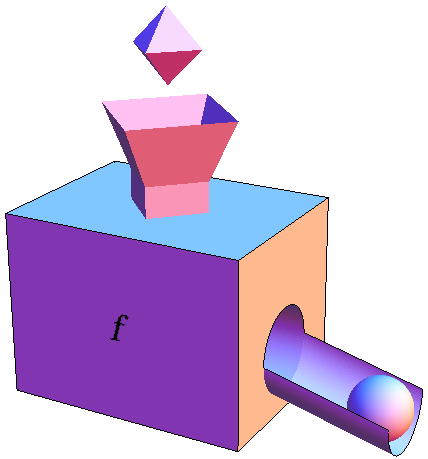
\includegraphics[width=\textwidth]{../Mathematik_1/Bilder/funktionen_maschinenmodell.png}
\end{minipage}
\begin{minipage}{0.56\textwidth}
	Die Maschine \(f\) produziert zu jedem \(x\in D\) ein \(y\in Z\). Den "\,Produktionsprozess"\, umkehren bedeutet eine Maschine \(f^{-1}\) zu finden, die jedem von \(f\) produzierten \(y\) sein Urbild, also seinen zugeh�rigen \(x\)-Wert, zuordnet, also so: 
\end{minipage}
\begin{minipage}{0.2\textwidth}
		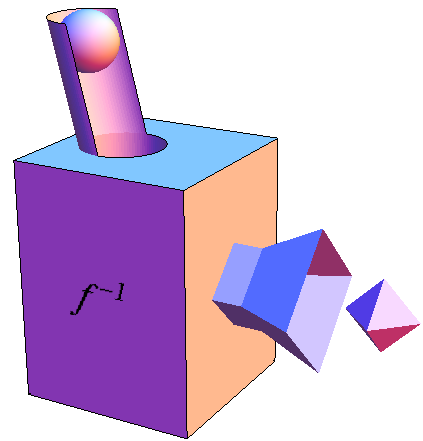
\includegraphics[width=\textwidth]{../Mathematik_1/Bilder/funktionen_umkehrfunktion_maschinenmodell.png}
\end{minipage}
\end{exabox}

Ist die Funktion als Graph gegeben, l��t sich die Frage nach der Existenz einer Umkehrfunktion leicht beantworten. Drehen wir den Graph so, dass die \(y\)-Achse waagerecht und die \(x\)-Achse senkrecht erscheint, und �berpr�fen, ob die gedrehte Figur eine Funktion ist:
\begin{itemize}
	\item[\(\Rightarrow\)] Falls ja, dann kann man \(f\) auf \(D\) umkehren!
	\item[\(\Rightarrow\)] Falls nein, dann gibt es keine Umkehrfunktion, zumindest nicht auf \(D\)! 
\end{itemize}
Was sagen Sie zum n�chsten Beispiel: besitzt die Funktion \(f: x\mapsto x^2\) eine Umkehrfunktion?\footnote{Die Normalparabel ist nicht umkehrbar, weil es kein eindeutiges "\,Zur�ck\"\, gibt.}
\begin{exabox}{Graphische L�sung: dreh den Graph um!}{ } 
	\begin{center}
		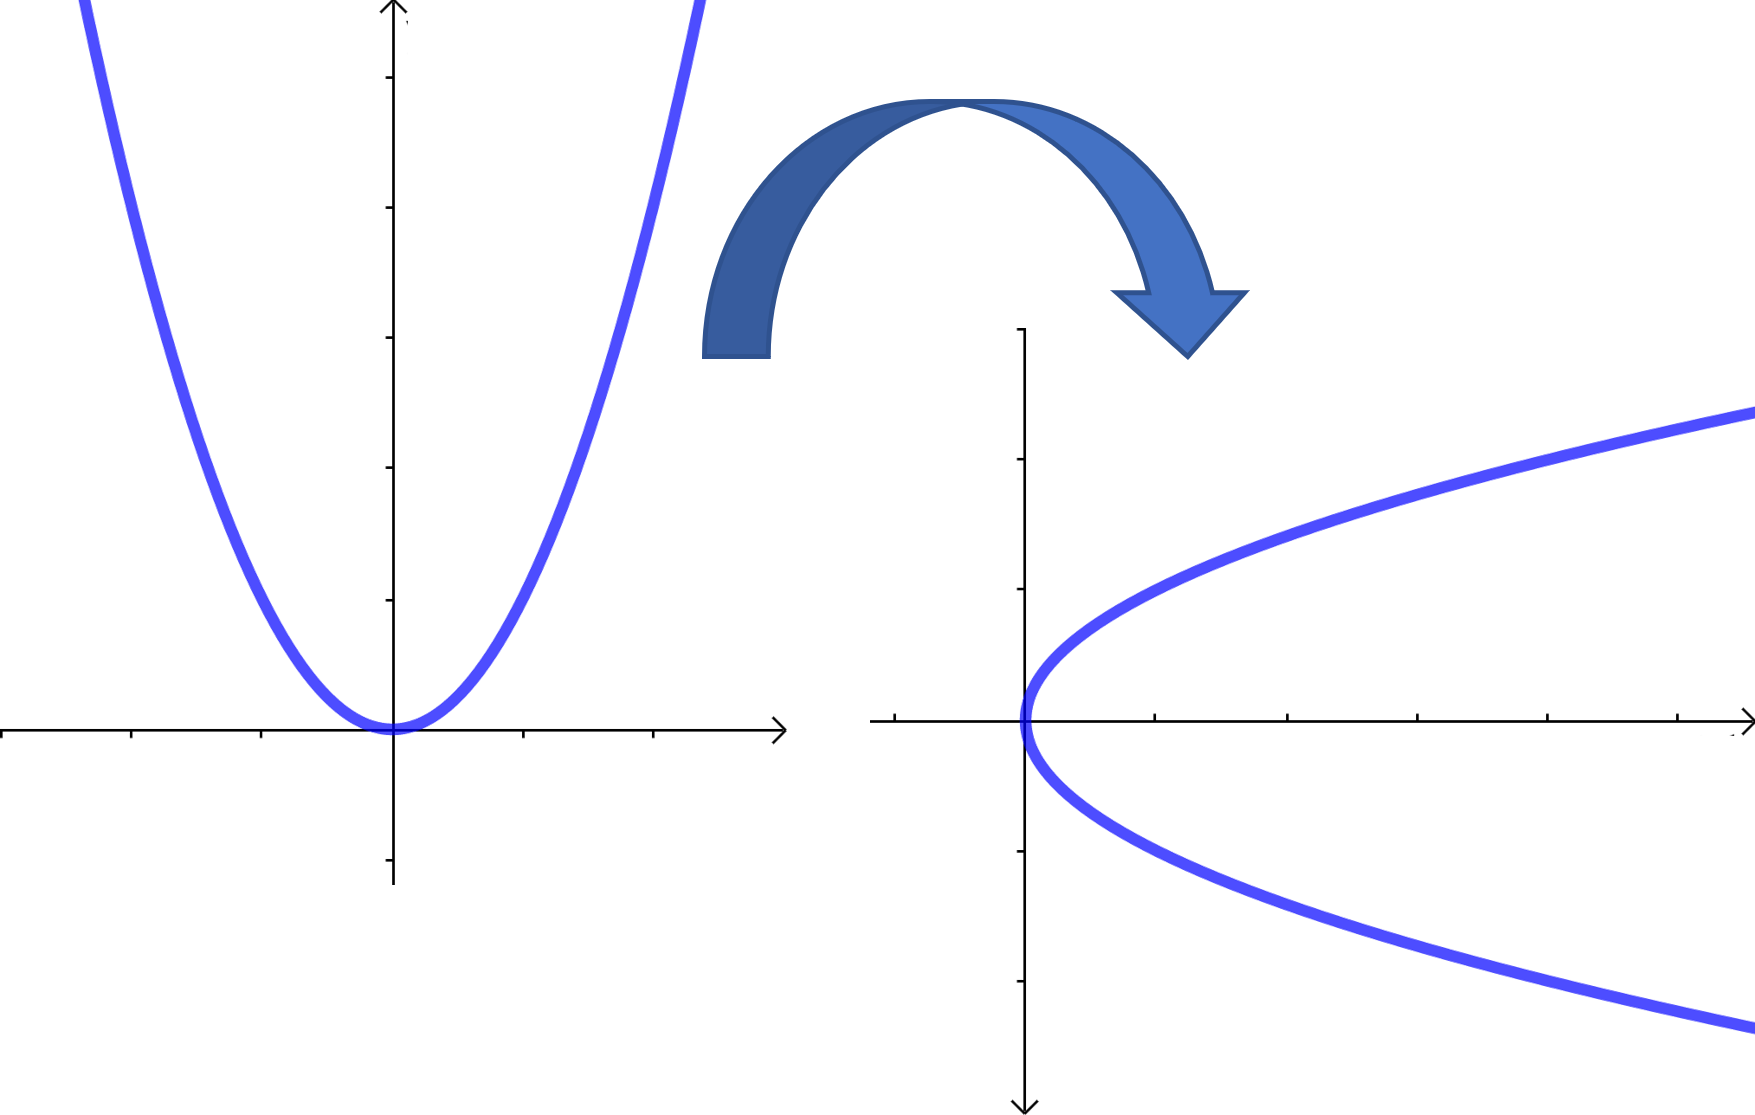
\includegraphics[width=0.6\textwidth]{../Mathematik_1/Bilder/funktionen_umkehrbarkeit_normalparabel_gedreht.png}
\end{center}
\end{exabox}

Die mathematischen Bedingungen daf�r, dass die gedrehte Figur der Graph einer Funktion ist, lauten :
  \begin{itemize}
	  \item Ein Funktionswert \(y\) im Zielmenge \(Z\) von \(f\) wird genau einmal erreicht. (Injektivit�t von \(f\) )
	  \item Jeder Funktionswert \(y\) im Bildmenge \(Z\) von \(f\) erreicht. (Surjektivit�t von \(f\) )
  \end{itemize}
  Gelten diese beiden Bedingungen, dann nennt man \(f\) bijektiv. F�r bijektive Funktionen l��t sich eine Umkehrfunktion bestimmen. In mathematischer Kurzschreibweise l��t sich die Bijektivit�t von \(f\) wie folgt definieren: 
\begin{defbox}{Existenz einer Umkehrfunktion}{ }
	\(f\) ist genau dann umkehrbar, wenn \(f\) bijektiv ist, wenn also gilt
  \begin{itemize}
	  \item $x,y\in D:\; f(x) = f(y)\, \Leftrightarrow\, x=y\,.$ (Injektivit�t)
	  \item $\forall\, y \in Z \, \exists\, x\in D:\; f(x) = y\;$ oder kurz \; $f(D) = Z$. (Surjektivit�t)
  \end{itemize}
\end{defbox}

\begin{exabox}{Injektivit�t? links ja, rechts nein!}{ } %Bild streng monotone Funktion ist umkehrbar
	\centering
	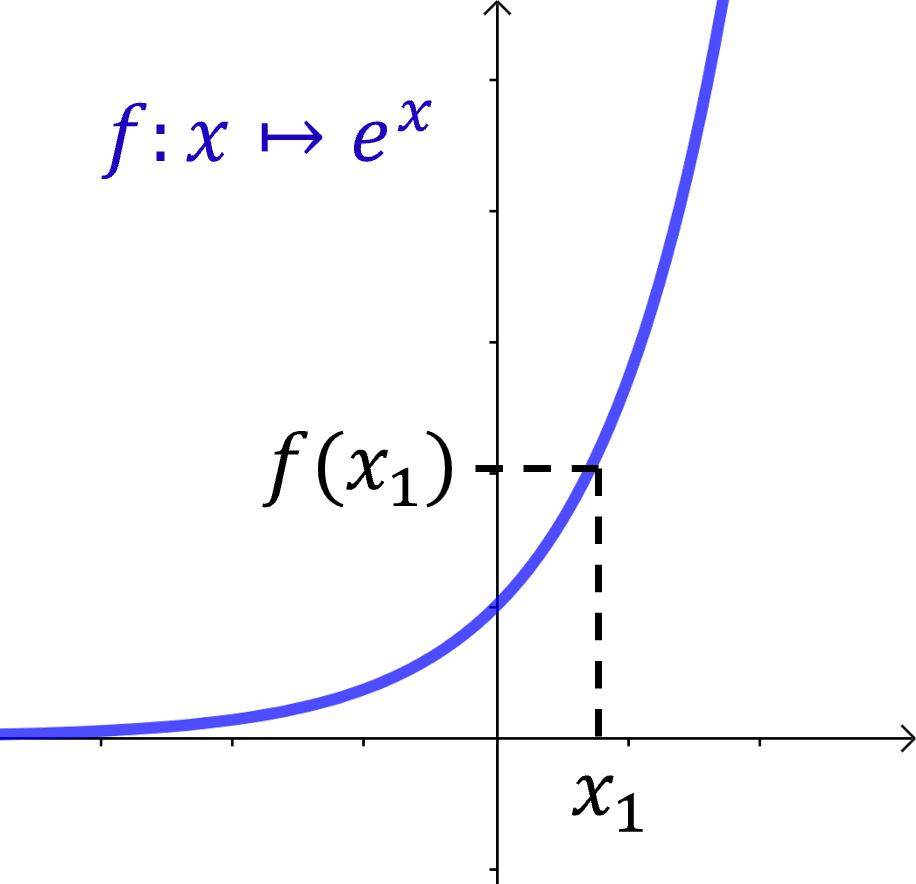
\includegraphics[width=0.25\textwidth]{../Mathematik_1/Bilder/funktionen_injektivitaet_exponentialfunktion.png}\hspace{3cm}
	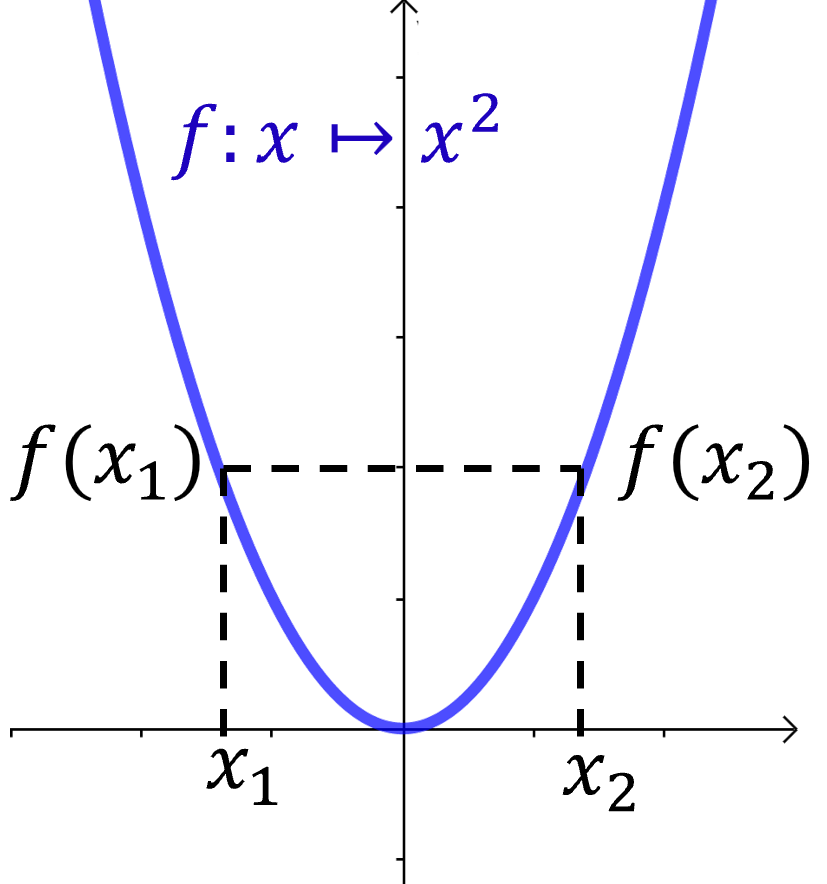
\includegraphics[width=0.25\textwidth]{../Mathematik_1/Bilder/funktionen_injektivitaet_quadratfunktion_gegenbeispiel.png}
\end{exabox}

%Die Funktionswerte \(y\) einer Funktion \(f: x\mapsto f(x) \)   Stellen Sie sich vor, dass Sie eine Funktionsabbildung gegeben haben, beispielsweise   finden Sie praktisch heraus, in dem Sie einen Funktionsgraphen um \(90\circ\) drehen und analysieren, ob die Figur, die Sie sehen eine Funktion ist oder nicht. Wir werden uns mit der
%Um  eine  Gleichung  wie $a+3=5$ nach $a$ aufzul�sen,  wendet  man  (strenggenommen) auf beide Seiten eine Funktion, n�mlich $x\mapsto x-3$, an:
%
%\begin{exabox}{Umkehrfunktion $\Rightarrow$ Aufl�sen einer Gleichung}{ }
%  $ a+ 3 = 5 \Leftrightarrow a+3-3 = 5-3 \Leftrightarrow a = 2\,.$
%\end{exabox}
%
%Um $e^b=7$ nach $b$ aufzul�sen wendet man entsprechend den nat�rlichen Logarithmus $x\mapsto \ln(x)$ an (warum ist das hier kein Problem?)
%
%\begin{exabox}{Umkehrfunktion $\Rightarrow$ Aufl�sen einer Gleichung}{ }
%  $e^b = 7 \Leftrightarrow \ln(\mathrm{exp}(b)) = \ln(7) \Leftrightarrow b = \ln(7)\,.$
%\end{exabox}

%Man sucht also Funktionen, welche die urspr�nglichen Funktionen wieder aufheben, sie umkehren:
%\begin{center}
%  \begin{tabular}{l|l}
%    Funktion & Idee Umkehrfunktion \\
%    \hline
%    $x\mapsto x+3$ & $x+3 \mapsto x$ \\
%    $x\mapsto \mathrm{exp}(x) $ &  $\mathrm{exp}(x) \mapsto x$ 
%  \end{tabular}
%\end{center}

Soweit zur Theorie, die spannendere Frage ist: wie bestimmen wir die Abbildungsvorschrift der \textbf{Umkehrfunktion} (\emph{inverse function})? 

\noindent{\textbf{Bemerkungen}}
\begin{itemize}
	\item Ist \(f\) eine \textbf{diskrete}, \textbf{bijektive} Funktion, gegeben als zweispaltige Tabelle, dann erh�lt man die Umkehrfunktion durch Vertauschen der beiden Spalten!\marginpar{Aufgabe} Die Tabelle l��t sich n�mlich einfach r�ckw�rts lesen und man erh�lt wieder eine Funktion: die Umkehrfunktion  $f^{-1}:Z\to D$. Der Definitionsbereich und die Zielmenge sind gegen�ber der Originalfunktion $f:D\to Z$ vertauscht. 
	\item Ist \(f\) eine \textbf{bijektive} Funktion, deren Funktionsabbildung gegeben ist, dann erh�lt man die Umkehrfunktion \(f^{-1}\), indem man die Abbildungsvorschrift \( y = f(x) \) nach \(x\) aufl�st. 
\end{itemize}


\begin{exabox}{Bestimmung der Umkehrfunktion}{ }
	\begin{itemize}
		\item $f:\mathbb R\to \mathbb R, \; x\mapsto \displaystyle{\frac12} \cdot x + 1 $ ist bijektiv, also 
			\begin{eqnarray*} 
					\begin{array}{lrlll}
						& y &=& \displaystyle{\frac12} \cdot x+1 &\; \| -1 \\[2ex]
						\Leftrightarrow & y-1 &=& \displaystyle{\frac12}\cdot x &\; \| \cdot 2 \\[2ex]
				\Leftrightarrow & 2\cdot y-2 &=& x &\;\Rightarrow  \; f^{-1}: \mathbb R\to \mathbb R, \; x\mapsto 2\cdot x-2\end{array}\end{eqnarray*}
			\item $f: (3,\infty)\to (0,\infty), \; x\mapsto \displaystyle{ \frac{2}{x-3}}$ ist bijektiv, also 
			\begin{eqnarray*} 
					\begin{array}{lrlll}
						&y &=&  \displaystyle{ \frac{2}{x-3}} & \|\cdot (x-3) \quad (x\not=3!) \\[2ex]
						\stackrel{x\not=3}{\Leftrightarrow} & (x-3) \cdot y &=& 2 & \| : y \quad (\not=0!) \\[2ex]
						\stackrel{y\not=0}{\Leftrightarrow} & x-3 &=& \displaystyle{\frac{2}{y} } &\|+3 \\[2ex]
						\Leftrightarrow & x &=& \displaystyle{\frac{2}{y} }+3 &  \;\Rightarrow \;  f^{-1}: (0,\infty) \to (3,\infty), \; x\mapsto \displaystyle{ \frac2x } +3
				\end{array}
			\end{eqnarray*}
	\end{itemize}
\end{exabox}

%\begin{exabox}{Bestimmung der Umkehrfunktionen}{ }
%	\begin{eqnarray*} 
%		f_1: x\mapsto x+3 & \Rightarrow & y = x+3 \Leftrightarrow x = y-3 \Rightarrow f_1^{-1}: x\mapsto x-3 \\ 
%		f_2: x\mapsto e^x & \Rightarrow & y = e^x \Leftrightarrow x = \ln(y) \Rightarrow f_2^{-1}: x \mapsto \ln(x) \,. 
%	\end{eqnarray*}
%\end{exabox}

\begin{theorembox}{Systematische Bestimmung der Umkehrfunktion}{ }
	\begin{enumerate}
		\item Bestimmung des Bildbereichs $W_f =f(D)\subset Z$ von $f$ (Surjektivit�t). 
		\item Bestimmung der Teilmenge $X\subseteq D$, auf der $f$ injektiv ist (Injektivit�t).
		\item L�sen der Gleichung $y=f(x)$ f�hrt auf $x=g(y)$. 
		\item Definition der Umkehrfunktion $ f^{-1}: W_f \to X, \; x\mapsto g(x)\,.$
	\end{enumerate}
\end{theorembox}

	\noindent\textbf{Bemerkungen:}
\begin{itemize} 
	\item Der Index $-1$ ist eine mathematische Notation -- sie hat nichts mit dem Kehrwert zu tun\footnote{Sp�ter bezeichnet $f^{42}$, dass die Funktion $f$ $42$-mal hintereinander anzuwenden ist, also $f^{42}(x)=f(f(\cdots 42-\mathrm{mal} \cdots f(x)\cdots))$. Die Notation mit $-1$ setzt diesen Gedanken fort und $f^0$ wird eingef�hrt als (komplizierte) Bezeichnung f�r die identische Abbildung: $f^0: x\mapsto x\,.$}.
	\item Wenn man zuerst die Funktion $f$ und dann auf das Resultat davon die dazugeh�rige Umkehrfunktion $f^{-1}$ anwendet (oder andersherum), dann erh�lt man die identische Abbildung \(\mathrm{id}: x\mapsto x\):
		\begin{theorembox}{$ \mathrm{id} = f \circ f^{-1} = f^{-1} \circ f$}{ }
  \begin{itemize}
	  \item[$\bullet$] $x \mapsto f^{-1}\big( f(x)\big) = x\,,$
	  \item[$\bullet$] $x \mapsto f\left( f^{-1}(x)\right) = x\,.$
\end{itemize}
\end{theorembox}
	\item In der praktischen  Ingenieurmathematik  k�mmert  man  sich  wenig  um  die Surjektivit�t. Denn ist eine Funktion injektiv, aber nicht surjektiv, kann man diesen Mangel leicht durch Anpassung der Zielmenge heilen. Zum Beispiel ist $f: \mathbb R \to \mathbb R, \, x\mapsto e^x$ nicht surjektiv, aber $f: \mathbb R \to (0,\infty), \, x\mapsto e^x$ ist surjektiv. 
\end{itemize}


Unter den folgenden Funktionen sind zwei, die umkehrbar sind. Wissen Sie welche?
\begin{itemize}
  \item $f_1: \mathbb R \to \mathbb R $ mit $x\mapsto \textnormal{kaufm\"annische Rundung von } x \textnormal{ auf eine Stelle nach dem Komma}$ 
  \item $f_2: \mathbb R \to \mathbb R$ mit $ x\mapsto x^2$
  \item $f_3: [0,8) \to \mathbb R$ mit $x\mapsto x^2$
  \item $f_4: [0,4) \to [0,16)$ mit $x\mapsto x^2$
  \item $f_5: \mathbb R \to \mathbb R$ mit $x\mapsto \sin(x)$
  \item $f_6: [-\pi/2,\pi/2] \to \mathbb R $ mit $x\mapsto \sin(x)$
  \item $f_7: [-\pi/2,\pi/2] \to [-1, 1] $ mit $ x \mapsto \sin(x)$
\end{itemize}
 \newpage % Funktionen Eigenschaften
\setcounter{exercise}{0} 
\ifintegriereaufgaben
\section*{Eigenschaften von Funktionen Aufgaben}\label{MA1-eigenschaften-von-funktionen-aufgaben}
	
	Regeln und Beispiele, die zur Bearbeitung der Aufgaben hilfreich sind, finden Sie im Skript\wennreferenzvorhanden{MA1-eigenschaften-von-funktionen}{ (Abschnitt \abschnittsverweis{MA1-eigenschaften-von-funktionen})} und, falls Sie nicht weiterkommen, schauen Sie \hyperref[MA1-eigenschaften-von-funktionen-loesungen]{hier}.
\else 
\section{Eigenschaften von Funktionen Aufgaben}\label{MA1-eigenschaften-von-funktionen-aufgaben}
	
	Regeln und Beispiele, die zur Bearbeitung der Aufgaben hilfreich sind, finden Sie im Skript und, falls Sie nicht weiterkommen, schauen Sie \hyperref[MA1-eigenschaften-von-funktionen-loesungen]{hier}.
\fi 

%\begin{theorembox}[Umkehrbarkeit]{}
%Es gilt:
%	\begin{itemize}
%		\item Eine Funktion $f:x\mapsto y$ mit der Definitionsmenge $D_f$ und der Wertemenge $W_f$ hei�t umkehrbar, falls es zu jedem $y\in W_f$ genau ein $x\in D_f$ mit $f(x)=y$ gibt.
%		\item Ist eine Funktion $f:x\mapsto y$ umkehrbar, so ist die umgekehrte Zuordnung $y\mapsto x$ eine Funktion. Diese hei�t Umkehrfunktion von $f$ und wird $f^{-1}$ bezeichnet. Ihre Definitionsmenge ist $W_f$ und ihre Wertemenge ist $D_f$.
%		\item Jede streng monotone Funktion $f$ ist umkehrbar. 
%	\end{itemize}
%\end{theorembox}

%\begin{theorembox}[Umkehrbarkeit]
%	Strenge Monotonie und damit Umkehrbarkeit kann man anhand der Ableitung diskutieren. Jede in einem Intervall $I$ differenzierbare Funktion $f$ mit $f'(x) > 0$  ($f'(x) < 0$) ist auf $I$ streng monoton steigend (fallend) und damit f�r alle $x\in I$ umkehrbar.
%\end{theorembox}

\begin{exercisebox}[Symmetrie]
  Welche der folgenden Funktionen ist gerade, welche ungerade?
  \begin{eqnarray*} \begin{array}{lll} 
		  (a)\; x\mapsto -2\cdot x^6 + 3\cdot x^2  \quad& (b)\; x\mapsto 2-3\cdot x^4 \quad &(c)\; x\mapsto 2-3\cdot x^3 \\[1ex]
		  (d)\; x\mapsto 3\cdot x^3-x+1 \quad & (e)\; x\mapsto x\cdot (2\cdot x^2 - \frac13\cdot  x^4) \quad & (f)\; x\mapsto (x-1)\cdot (x-2) \\[1ex]
		  (g)\; x\mapsto (x-1)^3+3\cdot x^2+1 \quad &(h)\; x\mapsto (1-3\cdot x^2)^2 & (i)\; x\mapsto (x-x^2)^2 
	  \end{array}
  \end{eqnarray*}
\end{exercisebox}


\begin{exercisebox}[Umkehrfunktion]
	Gegeben sei die (diskrete) Funktion $f:\{1,2,3,4\} \to \mathbb N$ mit der Wertetabelle 
	\begin{center}
\begin{tabular}{l|l|l|l|l}
$x$ & $1$ & $2$ & $3$ & $4$ \\ 
\hline
$f(x)$ & $9$ & $6$ & $7$ & $8$
\end{tabular}
\end{center}
Bestimmen sie die Umkehrfunktion $f^{-1}$.
\end{exercisebox}

\begin{exercisebox}[Umkehrfunktion]
  Auf welchen Intervallen ist $f$ umkehrbar? Bestimmen Sie $f^{-1}$ und geben Sie $D_{f^{-1}}$ an
  \begin{eqnarray*}
	  \begin{array}{lll} (a)\; f: x \mapsto 4\cdot x-x^2  & \quad \quad (b)\; f:x \mapsto \displaystyle{\frac{2\cdot x}{x-1}} & \quad \quad (c)\; f:x\mapsto x\cdot |x| \end{array}
  \end{eqnarray*}
\end{exercisebox}

\begin{exercisebox}[Anwendung: Verpackungsreduktion]
	Umweltbewusste Studenten behaupten: Bei Dosen-Limo ist die Verpackung teurer als der Inhalt. F�r die �berpr�fung treffen die Studenten folgende Annahmen: Die Dose ist ein Zylinder, dessen H�he doppelt so gro� ist wie sein Durchmesser. F�r den Hersteller kostet $1$ Liter Limo $15\,\mathrm{ct}$. Die Kosten f�r $1\,\mathrm{dm}^2$ Blech betragen $3 \,\mathrm{ct}$
  \begin{itemize}
	  \item[(a)] �berpr�fen Sie die Behauptung f�r den Dosenradius $3 \,\mathrm{cm}$.
	  \item[(b)] Ab welchem Dosenradius ist der Inhalt teurer als die Dose?
  \end{itemize}
\end{exercisebox}

\begin{exercisebox}[Anwendung: Kostenreduktion]
	Die Herstellungskosten eines Airbus-Seitenleitwerks aus Metall werden angen�hert durch \[ k_1: x\mapsto \frac{20\cdot x+5000}{x+50}\,,\] wobei $x$ die Anzahl der hergestellten Leitwerke und $k_1(x)$ eine willk�rliche Geldeinheit beschreibt. Nachdem $300$ Leitwerke hergestellt sind, wird erwogen, die Produktion auf Kunststoffleitwerke umzustellen. Die St�ckkosten betragen dann n�herungsweise \[k_2:x\mapsto \frac{15\cdot x-2500}{x-250}\,, \quad x>300\,.\]
  \begin{enumerate}
  	\item Zeichnen Sie die beiden Graphen, zum Beispiel mit Hilfe von Geogebra o.�..
	\item Wie verhalten sich die St�ckkosten bei sehr gro�en Produktionszahlen?
	\item Ab welcher St�ckzahl ist das Kunststoffleitwerk billiger?
  \end{enumerate}
\end{exercisebox}
 \newpage 
\setcounter{satz}{0} \setcounter{def}{0} \setcounter{exa}{0}  \section{Lineare Funktionen}\label{MA1-lineare-funktionen}

\begin{table}[H]
  \centering
  \begin{tabularx}{\textwidth}{p{0.9\textwidth} p{0.1\textwidth}}
    \toprule
	  \multicolumn{2}{c}{\textbf{�bersicht �ber Lernziele und Voraussetzungen}}\\
    \midrule
    \textbf{Lernziele} &\\[.5\normalbaselineskip]
    \tabitem lineare Funktionen in verschiedenen Darstellungsformen angeben und ineinander �berf�hren: &\\
    \hspace{0.7cm}\tabitem Achsenabschnittsform &\\
    \hspace{0.7cm}\tabitem Zwei-Punkte-Form &\\
    \hspace{0.7cm}\tabitem Punkt-Steigungs-Form &\\
    \tabitem st�ckweise definierte Funktionen lesen und interpretieren &\\
    \tabitem eine gegebene Messreihe durch lineare Interpolation mit einem linearen Spline beschreiben &\\
    \tabitem Interpolation und lineare Regression voneinander unterscheiden &\\
    \tabitem f�r eine Messreihe eine Ausgleichsgerade mittels linearer Regression bestimmen &\\
    \midrule
	  \textbf{Voraussetzungen} \\[.5\normalbaselineskip]
	  \tabitem Grundrechenarten & \abschnittsverweis{MA1-zahlenmengen}\\
	  \tabitem �quivalenzumformungen & \abschnittsverweis{MA1-aequivalenzumformungen}\\
	  \tabitem Definition einer Funktion & \abschnittsverweis{MA1-funktionen}\\
    \bottomrule
  \end{tabularx}
\end{table}

\ifintegriereaufgaben \noindent �bungsaufgaben zum Thema finden Sie hier: \hyperref[MA1-lineare-funktionen-aufgaben]{Aufgaben}
\vspace{0.3cm}
\hrule
\fi

\subsection{Lineare Funktionen}

Funktionen der Art $f: \mathbb R \to \mathbb R$ mit $x\mapsto 2\cdot x+3$ hei�en \textbf{linear}\footnote{In der Schulmathematik und elementaren Analysis werden Funktionen der Form \(f(x)=mx+b\) �blicherweise als lineare Funktionen bezeichnet. Im Sinne der linearen Algebra handelt es sich f�r \(b\neq0\) um affine Abbildungen; eine lineare Abbildung muss insbesondere \(f(0)=0\) erf�llen.}

Der Graph einer linearen Funktion ist eine Gerade, aber keine vertikale Gerade\footnote{Eine vertikale Gerade kann nicht Graph einer Funktion \(x\mapsto f(x)\) sein, da zu derselben \(x\)-Koordinate mehrere \(y\)-Werte geh�ren w�rden.}
In der Form

$$
f(x)=m \cdot x+b
$$

beschreibt \(m\) die \textbf{Steigung} der Geraden und \(b=f(0)\) ihren Schnittpunkt mit der \(y\)-Achse. Je nachdem, welche Informationen �ber eine Gerade gegeben sind, sind jedoch unterschiedliche Darstellungsformen zweckm��ig.

\begin{itemize}
	\item Angenommen \(f\) schneidet die $x$-Achse an der Stelle $a\in D$ mit \(a\not=0\) und \(f\) schneidet die $y$-Achse im Punkt $(0,b)\in D\times Z$ mit \(b\not=0\), dann kann man die Abbildungsvorschrift der lineare Funktion in \textbf{Achsenabschnittsform} angeben:
		\[ 
			f(x) = \displaystyle{-\frac{b}{a}}\cdot x + b.
  \]
Dass diese Gleichung tats�chlich richtig ist, kann man so sehen: sie beschreibt eine Gerade und stimmt f�r die beiden Schnittpunkte mit den Achsen. Eine  andere  Gerade  als  die  gesuchte  w�rde  aber  nicht  durch  diese  beiden Schnittpunkte verlaufen. 

\item F�r zwei voneinander verschiedene Punkte  $(x_1|y_1)$ und $(x_2|y_2)$, die auf einer nichtvertikalen Geraden liegen, ist das Verh�ltnis von \(y_2 - y_1\) zu \(x_2 - x_1\) immer gleich! Der Wert wird \textbf{Steigung der Gerade} genannt:
	\[ 
  m = \displaystyle{\frac{y_2-y_1}{x_2-x_1}}.
  \]
Kennt man die Steigung \(m\) der Gerade und einen Punkt \( (x_1|y_1)\) auf der Gerade, dann ist die Gerade eindeutig bestimmt. Die \textbf{Punkt-Steigungs-Form} liefert die Abbildungsvorschrift: 
\[ 
	f(x) = m\cdot (x-x_1) + y_1.
\]
\item Kennt man anstatt der Steigung einen weiteren Punkt, gibt man die Gerade in \textbf{Zwei-Punkte-Form} an:

	\[ f(x) = \displaystyle{\frac{y_2-y_1}{x_2-x_1}}\cdot (x-x_1) + y_1.\]
	\end{itemize}


\begin{exabox}{Lineare Funktion \(f: x\mapsto 2\cdot x+3\)}{ }
\begin{minipage}{0.3\textwidth}
	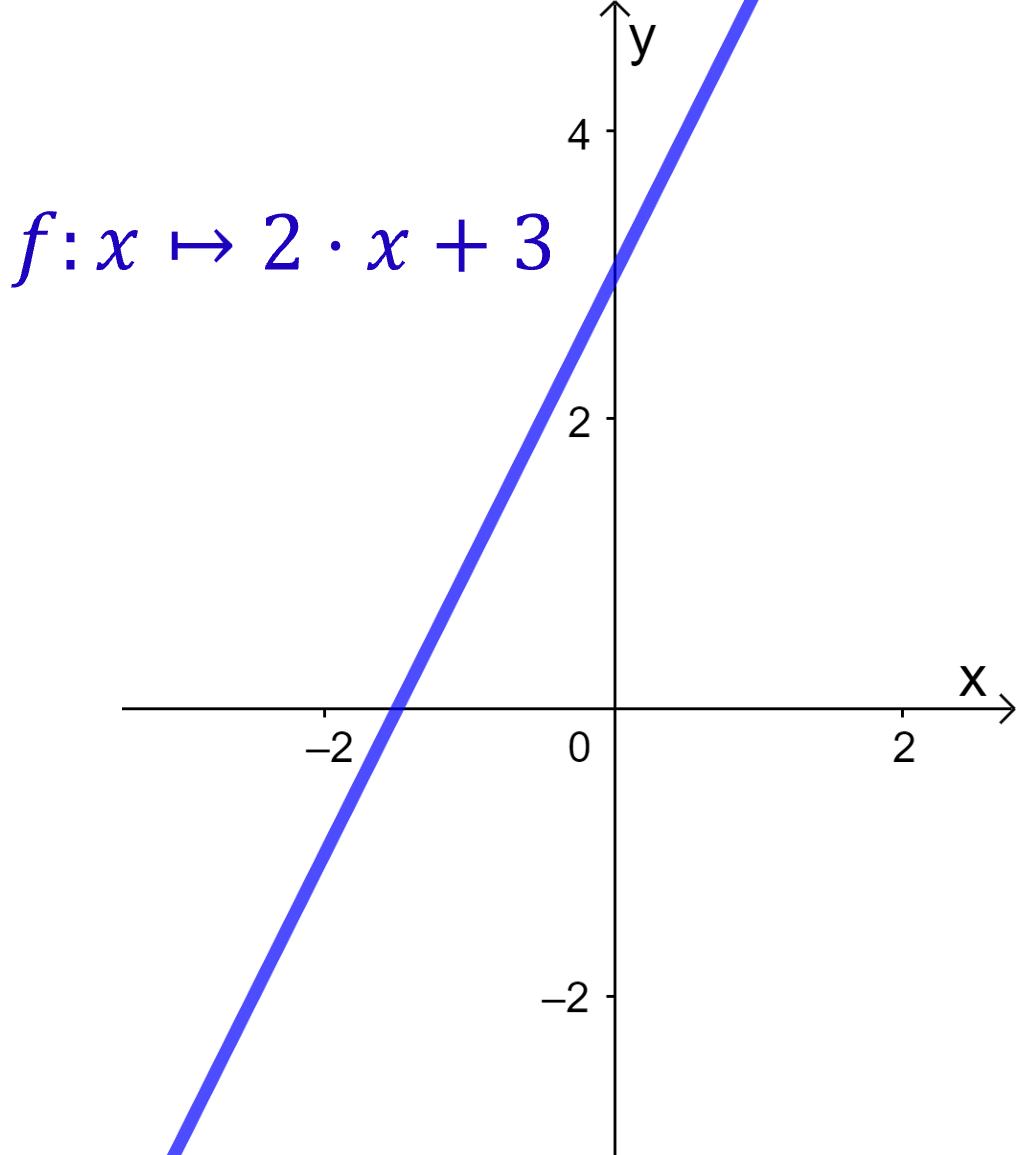
\includegraphics[width=\textwidth]{../Mathematik_1/Bilder/lineare_funktionen_gerade_zwei_x_plus_drei.png}
	\end{minipage}
	\begin{minipage}{0.7\textwidth}
		Unterschiedliche Darstellungen f�r \(f\):
		\begin{itemize}
			\item Achsenabschnitt-Form:
				\[a=-\frac32, \; b = 3: \quad f(x) = - \dfrac{3}{-\frac32}\cdot x + 3 = 2\cdot x+3 \]
			\item Punkt-Steigungs-Form:
				\[m=2, \; P(1|5):\quad f(x) = 2\cdot \left( x- 1\right) + 5 = 2\cdot x+3 \]
			\item Zwei-Punkte-Form:
				\[P_1(0|3),\; P_2(1|5): \quad f(x) =  \dfrac{3-5}{0-1}\cdot \left( x- 1\right) + 5  = 2\cdot x+3\,.\]
		\end{itemize}
	\end{minipage}
\end{exabox}

\subsection{Interpolation mit Linearen Funktionen}

In einer der folgenden Anwendungen wird der Begriff "\,st�ckweise definierte Funktion"\, benutzt:

\begin{defbox}{St�ckweise definierte Funktion}{ }
Eine Funktion hei�t \textbf{st�ckweise definiert} (\emph{piecewise defined}), wenn f�r verschiedene Teilbereiche ihres Definitionsbereichs unterschiedliche Abbildungsvorschriften gelten.

Beispielsweise kann eine Funktion die Form

$$
f(x)=
\begin{cases}
f_1(x), & x\in D_1,\\
f_2(x), & x\in D_2,\\
\vdots\\
f_n(x), & x\in D_n
\end{cases}
$$

besitzen, wobei

$$
D=D_1\cup D_2\cup \cdots \cup D_n.
$$

Dabei muss f�r jedes \(x\in D\) eindeutig festgelegt sein, welche Abbildungsvorschrift gilt.
	
	%Von einer st�ckweise definierten Funktion \(f: D\to \mathbb R\) ist dann die Rede, wenn man den Definitionsbereich in \(N-1\) Intervalle \[I_k= [x_k, x_{k+1}], \; x_k < x_{k+1}, \; k=1,\cdots, N-1, \] aufteilen kann, also \[ D = \bigcup\limits_{k=1}^{N-1} I_k = [x_1, x_N]\,,\] und wenn sich auf jedem der Intervalle \(I_k\) eine geschlossene Abbildungsformel angeben l��t: \[ f:x\mapsto \begin{cases} f_1(x), \quad x\in I_1,\\[2ex] f_2(x),\quad x\in I_2, \\[1ex] \vdots \\ f_{N-1}(x), \quad x\in I_{N-1}\,.\end{cases}\] 
\end{defbox}
	%Die Frage, ob eine st�ckweise definierte Funktion auf ihrem Definitionsbereich stetig oder sogar differenzierbar ist, h�ngt offensichtlich damit zusammen, wie glatt die Funktion von einem Intervall zum anderen Intervall �bergeht. 
Der Prototyp einer st�ckweise definierten Funktion ist die Betragsfunktion:\marginpar{Aufgabe} 
	\begin{exabox}{Betragsfunktion}{ }
		$ f:x\mapsto |x| = \begin{cases} x, &\quad x \in [0, \infty)\,, \\ -x, &\quad x\in (-\infty,0)\,.\end{cases} $
\end{exabox}

Liegt eine Messreihe vor, so wurde eine Gr��e \(y\) f�r verschiedene Werte einer anderen Gr��e \(x\) bestimmt. Ein Beispiel ist die elektrische Leitf�higkeit eines Metallblocks in Abh�ngigkeit von seiner Temperatur.

Die Messdaten bestehen aus \(N\) Messpunkten

$$
\{(x_i,y_i):i=1,\dots,N\}.
$$

Dabei seien die Messstellen aufsteigend geordnet $ x_1<x_2<\dots<x_N$.

Soll eine Funktion konstruiert werden, deren Graph durch s�mtliche Messpunkte verl�uft, spricht man von einer \textbf{Interpolation} (\emph{interpolation}). Eine besonders einfache M�glichkeit besteht darin, jeweils zwei benachbarte Messpunkte durch eine Gerade zu verbinden. Auf jedem Intervall

$$
I_k=[x_k,x_{k+1}]
$$

wird also die Zwei-Punkte-Form einer Geraden verwendet. Auf diese Weise entsteht ein \textbf{linearer Spline} (\emph{linear spline}).

%Nehmen wir uns liegt eine Messreihe vor: eine physikalische Gr��e \(y\) wurde in Abh�ngigkeit einer anderen Gr��e \(x\) gemessen\footnote{Zum Beispiel die Leitf�higkeit eines Metallblocks in Abh�ngigkeit von seiner Temperatur.}. Die Messdaten bestehen dann also aus einer Menge von \(N\) Messpunkten \[ \left\{ \left( x_i| y_i\right), \; x_i, y_i \in \mathbb R,\; i=1,\dots,N\right\} \] und zur Analyse der Daten suchen wir eine Funktion, deren Graph die Messpunkte durchl�uft.\marginpar{Aufgabe} Wir suchen eine Funktion, die die Daten \textbf{interpoliert}. Eine Idee ist die folgende: zwischen zwei aufeinanderfolgenden Messwerten wird linear interpoliert --  auf diese Weise wird ein \textbf{linearer Spline} konstruiert. Die Details fasst die folgende Regel zusammen.  

\begin{defbox}{Linearer Spline}{ }
	Es seien \(N\) Messpunkte \( \{(x_i| y_i),\; x_i, y_i \in \mathbb R\,, \; i=1,\cdots,N, \text{ und } x_1<x_2< \cdots <x_N \} \) gegeben. Mit 
$$
I_k=[x_k,x_{k+1}], \; k=1,\ldots,N-1, 
$$
lautet der lineare Spline
	
	\begin{eqnarray*}
		f: [x_1,x_N] \to\mathbb R,\; x\mapsto \begin{cases} \displaystyle{\frac{y_2-y_1}{x_2-x_1}}\cdot (x-x_1) + y_1, \quad x\in I_1\,,\\[2ex]  \displaystyle{\frac{y_3-y_2}{x_3-x_2}}\cdot (x-x_2) + y_2, \quad x\in I_2\,,\\  \vdots \\  \displaystyle{\frac{y_N-y_{N-1}}{x_N-x_{N-1}}}\cdot (x-x_{N-1}) + y_{N-1}, \quad x\in I_{N-1}\,.\end{cases}
	\end{eqnarray*}
\end{defbox}

Ein linearer Spline ist nichts anderes als die wiederholte Anwendung der Zwei-Punkte-Form auf benachbarte Messpunkte.

\subsection{Lineare Regression }

Bei einer Interpolation wird verlangt, dass der Graph der konstruierten Funktion s�mtliche Messpunkte exakt durchl�uft. F�r Messdaten ist diese Forderung jedoch nicht immer sinnvoll. Messwerte sind h�ufig mit Messfehlern und anderen Unsicherheiten behaftet, sodass kleine Abweichungen einzelner Punkte nicht unbedingt Teil des zugrunde liegenden funktionalen Zusammenhangs sind.

In einer solchen Situation wird statt einer exakt interpolierenden Funktion eine Funktion gesucht, welche die Gesamtheit der Messdaten m�glichst gut beschreibt. Soll dieser Zusammenhang durch eine Gerade modelliert werden, f�hrt dies zur \textbf{linearen Regression} (\emph{linear regression}).

Gesucht ist eine lineare Funktion \(f:x\mapsto mx+b\), f�r welche die Summe der quadrierten vertikalen Abweichungen von den Messwerten minimal wird. 

Die \textbf{Abweichung} oder das \textbf{Residuum} (\emph{residual}) des \(i\)-ten Messwerts von der Geraden betr�gt

$$ r_i=f(x_i) - y_i = m\cdot x_i+b-y_i. $$

Bei der Bestimmung der linearen Regression werden \(m\) und \(b\) so gew�hlt, dass die Summe aller quadrierten Abweichungen

$$ r_1^2+\dots+r_N^2 $$

m�glichst klein wird: 

\[ \sum\limits_{i=1}^N \left( m \cdot x_i + b - y_i \right)^2 \stackrel{!}{=} \min \,.\]
F�r verschiedene Messstellen \(x_i\) ist die Aufgabe eindeutig l�sbar mit expliziten Formeln f�r die optimalen Werte von $m$ und $b$:\marginpar{Aufgabe} 

\begin{theorembox}{Ausgleichsgerade (lineare Regression oder Bestapproximation)}{ }
	Die Ausgleichsgerade \[ f: x\mapsto m\cdot x + b \] f�r $N$ verschiedene Messpunkte $\{ (x_1, y_1), (x_2,y_2), \dots, (x_N, y_N)\}$ mit $x_1 < x_2 < \cdots < x_n$ besitzt die Steigung  
	\begin{eqnarray*} 
		m = \frac{\sum\limits_{i=1}^N (x_i - \langle x\rangle ) \cdot (y_i - \langle y\rangle ) }{ \sum\limits_{i=1}^N (x_i - \langle x \rangle )^2 }
		\end{eqnarray*}
		und den \(y\)-Achsenabschnitt 
		\begin{eqnarray*}
		b = \langle y \rangle - m \cdot \langle x\rangle\,.
	\end{eqnarray*} 
	Die spitzen Klammern $\langle \cdot  \rangle $ bezeichnen Mittelwerte, also
	\begin{eqnarray*}
		\langle x \rangle = \frac{1}{N} \cdot \sum\limits_{i=1}^N x_i\,, \quad \langle y \rangle = \frac{1}{N}\cdot \sum\limits_{i=1}^N y_i\,.
	\end{eqnarray*}
\end{theorembox}

\noindent{\textbf{Bemerkung:}}
\begin{itemize}
	\item Die Ausgleichsgerade verl�uft damit durch den Punkt $ \big(\langle x\rangle,\langle y\rangle\big), $ also durch den Schwerpunkt der Messpunkte.
	\item Die Ausgleichsgerade interpoliert alle Messpunkte, wenn die Messpunkte exakt auf einer Geraden liegen.
	\item Die Ausgleichsgerade reagiert sensitiv auf \textbf{Ausrei�er} in der Messreihe, weil die Abst�nde quadriert werden. 
\end{itemize}

\begin{exabox}{Lineare Regression}{}

Gegeben seien die drei Messwerte

$$
(1,2),\qquad (2,3),\qquad (3,5).
$$

Gesucht ist daher eine Ausgleichsgerade, die die drei Messwerte im Sinne der kleinsten Quadrate m�glichst gut beschreibt.

\begin{itemize} 
	\item Zun�chst werden die Mittelwerte der \(x\)- und \(y\)-Werte bestimmt:

$$
\langle x\rangle = \frac{1+2+3}{3} = 2, \quad \langle y\rangle = \frac{2+3+5}{3} = \frac{10}{3}.
$$

\item Die Steigung der Ausgleichsgerade l�sst sich nun berechnen:

$$
\begin{aligned}
m
&=
\frac{
\displaystyle
\sum_{i=1}^3
(x_i-\langle x\rangle)
(y_i-\langle y\rangle)
}{
\displaystyle
\sum_{i=1}^3
(x_i-\langle x\rangle)^2
}
\\[1ex]
&=
\frac{
(1-2)\left(2-\frac{10}{3}\right)
+
(2-2)\left(3-\frac{10}{3}\right)
+
(3-2)\left(5-\frac{10}{3}\right)
}{
(1-2)^2+(2-2)^2+(3-2)^2
}
\\[1ex]
&=
\frac{
\frac43+0+\frac53
}{
1+0+1
}
=
\frac{3}{2}.
\end{aligned}
$$

\item Damit ergibt sich f�r den \(y\)-Achsenabschnitt 

$$
b
=
\frac{10}{3}
-
\frac32\cdot2
=
\frac13.
$$
\end{itemize}

Die gesuchte Ausgleichsgerade lautet damit $f(x)=\frac32x+\frac13$.

	\begin{minipage}{0.5\textwidth}
		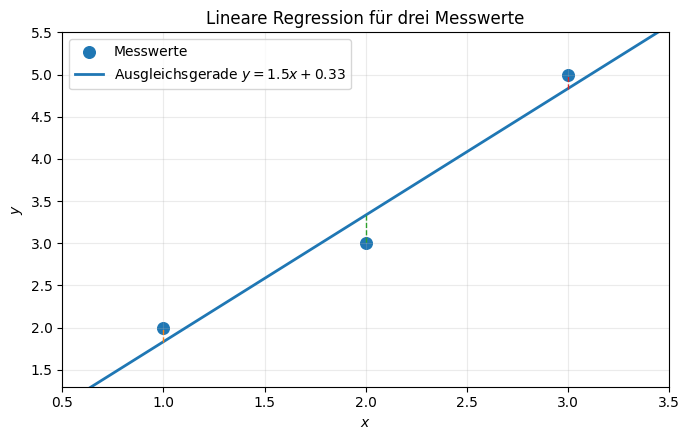
\includegraphics[width=\textwidth]{../Mathematik_1/Bilder/lineare_regression_drei_messwerte.png}
\end{minipage}
\begin{minipage}{0.5\textwidth}
	\begin{itemize}
		\item Im Unterschied zu einer Interpolation verl�uft die Ausgleichsgerade im Allgemeinen nicht durch die Messpunkte. 
		\item Die gestrichelten vertikalen Linien in der Abbildung zeigen die Abweichungen zwischen den Messwerten und den zugeh�rigen Werten der Ausgleichsgeraden.
	\end{itemize}
\end{minipage}

\end{exabox}
 \newpage % Lineare Funktionen
\setcounter{exercise}{0} 
\ifintegriereaufgaben
\section*{Lineare Funktionen Aufgaben}\label{MA1-lineare-funktionen-aufgaben}
	
	Regeln und Beispiele, die zur Bearbeitung der Aufgaben hilfreich sind, finden Sie im Skript\wennreferenzvorhanden{MA1-lineare-funktionen}{ (Abschnitt \abschnittsverweis{MA1-lineare-funktionen})} und, falls Sie nicht weiterkommen, schauen Sie \hyperref[MA1-lineare-funktionen-loesungen]{hier}.

\else
\section{Lineare Funktionen Aufgaben}\label{MA1-lineare-funktionen-aufgaben}
	
	Regeln und Beispiele, die zur Bearbeitung der Aufgaben hilfreich sind, finden Sie im Skript und, falls Sie nicht weiterkommen, schauen Sie \hyperref[MA1-lineare-funktionen-loesungen]{hier}.
\fi 

\begin{exercisebox}[Abbildungsvorschrift] %Andreas
	Bestimmen Sie die Abbildungsvorschrift (Funktionsgleichung) in der Form \[ f(x) = m\cdot x + b\] einer linearen Funktion durch die Punkte \( (1,5| 2)\) und \( (-3|3)\).
\end{exercisebox}

\begin{exercisebox}[Umkehrfunktion]
	F�r welche reellen Werte von \(m\) und \(b\) ist die lineare Funktion $f: x\mapsto m\cdot x+b$ umkehrbar? 
\end{exercisebox}

\begin{exercisebox}[Abbildungsvorschrift] %Lovis
	Die durch die Gleichung \( x +3y= 8\) beschriebene Gerade im \(\mathbb R^2\) wird um zwei Einheiten nach rechts und um eine Einheit nach oben geschoben. Geben Sie die Abbildungsvorschrift f�r die verschobene Gerade an.  
\end{exercisebox}

\begin{exercisebox}[Betragsfunktion] %Lovis
	Skizzieren Sie die Menge \( \{ (x,y) \in \mathbb R^2: y<1+|x|\}\). Kennzeichnen Sie, ob die R�nder dazu geh�ren oder nicht. 
\end{exercisebox}

\begin{exercisebox}[Betragsfunktion] % LS p.21
		Stellen Sie die folgenden Funktionen ohne Betragszeichen dar. Zeichnen Sie den Graph: 
  \begin{eqnarray*}
	  \begin{array}{llll}
		  (a)\; f:x \mapsto 2\cdot |x| & \quad (b)\; f:x \mapsto |2-x| & \quad (c)\; f:x \mapsto |2+x| &\quad (d)\; f:x \mapsto x-|x|
	  \end{array}
  \end{eqnarray*}
\end{exercisebox}

\begin{exercisebox}[Anwendung: Interpolation] % Andreas
	Gegeben sind die Messpunkte $(x_i,y_i), \; i= 0,1,2,3,$ mit $(-1,5| 2),(-0,25| 3,5),(0,5| 3,3),(1,2| 2,8)$. Bestimmen Sie den linearen Spline und werten Sie ihn am Punkt $x= 0,2$ aus. Welchen Wert erhalten Sie?
\end{exercisebox}

\begin{exercisebox}[Anwendung: Ausgleichsgerade] %Lucy
	Gegeben sind die Messpunkte $(x_i,y_i), \; i= 0,1,2,3,$ mit $(-1,5| 2),(-0,25| 3,5),(0,5| 3,3),(1,2| 2,8)$. Bestimmen Sie die Ausgleichsgerade und werten Sie ihn am Punkt $x= 0,2$ aus. Welchen Wert erhalten Sie?
\end{exercisebox}

\begin{exercisebox}[Anwendung: Dimensionierung Solarzellen] %LS p.21
	Sonnenkollektoren wandeln Lichtenergie in W�re um, die an den Warmwasserspeicher abgef�hrt wird. Die ben�tigte Kollektorfl�che h�ngt linear vom Volumen des Speichers ab. Bei einer Speichertemperatur von $45^\circ \mathrm{C}$ wird f�r $200$ Liter eine Kollektorfl�che von $3\mathrm{m}^2$, f�r eine $500$ Liter $7\mathrm{m}^2$ empfohlen. Pro Person wird mit einem Verbrauch von $50$ Liter Warmwasser am Tag gerechnet. Das Speichervolumen sollte $50\%$ �ber dem Verbrauch liegen. 
  \begin{enumerate}
    \item Bestimmen Sie die Funktion, die der Personenanzahl die Kollektorfl�che zuordnet.
    \item Wie gro� sollte die Kollektorfl�che bei einem $4$-Personen Haushalt sein?
    \item F�r wie viele Personen reicht eine Kollektorfl�che von $8\mathrm{m}^2$?
  \end{enumerate}
\end{exercisebox}


%\begin{exercisebox}[Elastizit�t]
%\end{exercisebox}
%
%\begin{exercisebox}[Federkraft]
%\end{exercisebox}
 \newpage 
\setcounter{satz}{0} \setcounter{def}{0} \setcounter{exa}{0}  

\section{Potenzfunktionen und Wurzelfunktionen}\label{MA1-potenz-und-wurzelfunktionen}

\begin{table}[H]
  \centering
  \begin{tabularx}{\textwidth}{p{0.9\textwidth} p{0.1\textwidth}}
    \toprule
	  \multicolumn{2}{c}{\textbf{�bersicht �ber Lernziele und Voraussetzungen}}\\
    \midrule
	  \textbf{Lernziele} &\\[.5\normalbaselineskip]
	  \tabitem Potenzfunktionen und Wurzelfunktionen skizzieren &\\
	  \tabitem Monotonie und Symmetrie einer Potenzfunktion charakterisieren &\\
\tabitem Wurzelfunktionen als Umkehrfunktionen geeigneter Potenzfunktionen vestehen &\\
\tabitem Definitionsbereiche von Wurzelfunktionen bestimmen &\\
\tabitem Gleichungen mit Potenzen und Wurzeln unter Beachtung des Definitionsbereichs l�sen &\\
\tabitem Potenzrechenregeln mit ganzzahligem und gebrochenzahligem Exponenten anwenden &\\
    \midrule
	  \textbf{Voraussetzungen} \\[.5\normalbaselineskip]
	  \tabitem Grundrechenarten & \abschnittsverweis{MA1-zahlenmengen}\\
	  \tabitem �quivalenzumformungen & \abschnittsverweis{MA1-aequivalenzumformungen}\\
	  \tabitem Injektivit�t, Bijektivit�t, Umkehrbarkeit  & \abschnittsverweis{MA1-funktionen}\\
    \bottomrule
  \end{tabularx}
\end{table}

 \ifintegriereaufgaben \noindent �bungsaufgaben zum Thema sind hier: \hyperref[MA1-potenz-und-wurzelfunktionen-aufgaben]{Aufgaben}
\vspace{0.3cm}
\hrule
 \fi

\subsection{Potenzfunktionen} 


Eine Funktion der Form
\[
f:\mathbb R\to\mathbb R,\qquad x\mapsto x^n,
\]
mit \(n\in\mathbb N^+\) hei�t Potenzfunktion (\emph{power function}). Der Definition \underline{Definitionsbereich}\randverweis{MA1-funktionen} aller dieser Potenzfunktionen \footnote{Auch Funktionen wie \(x\mapsto x^{-1/5}\) oder \(x\mapsto x^\pi\) geh�ren zu allgemeineren Potenzfunktionen.  Ihre Definitionsbereiche erfordern jedoch zus�tzliche �berlegungen: \(x^{-1/5}\) ist bei \(x=0\) nicht definiert, w�hrend \(x^\pi\) im Reellen f�r negative \(x\) nicht definiert ist.} ist \(\mathbb R\).

\begin{theorembox}{Monotonie und Symmetrie von Potenzfunktionen mit geradem Exponenten}{ }
	\begin{minipage}{0.35\textwidth}
	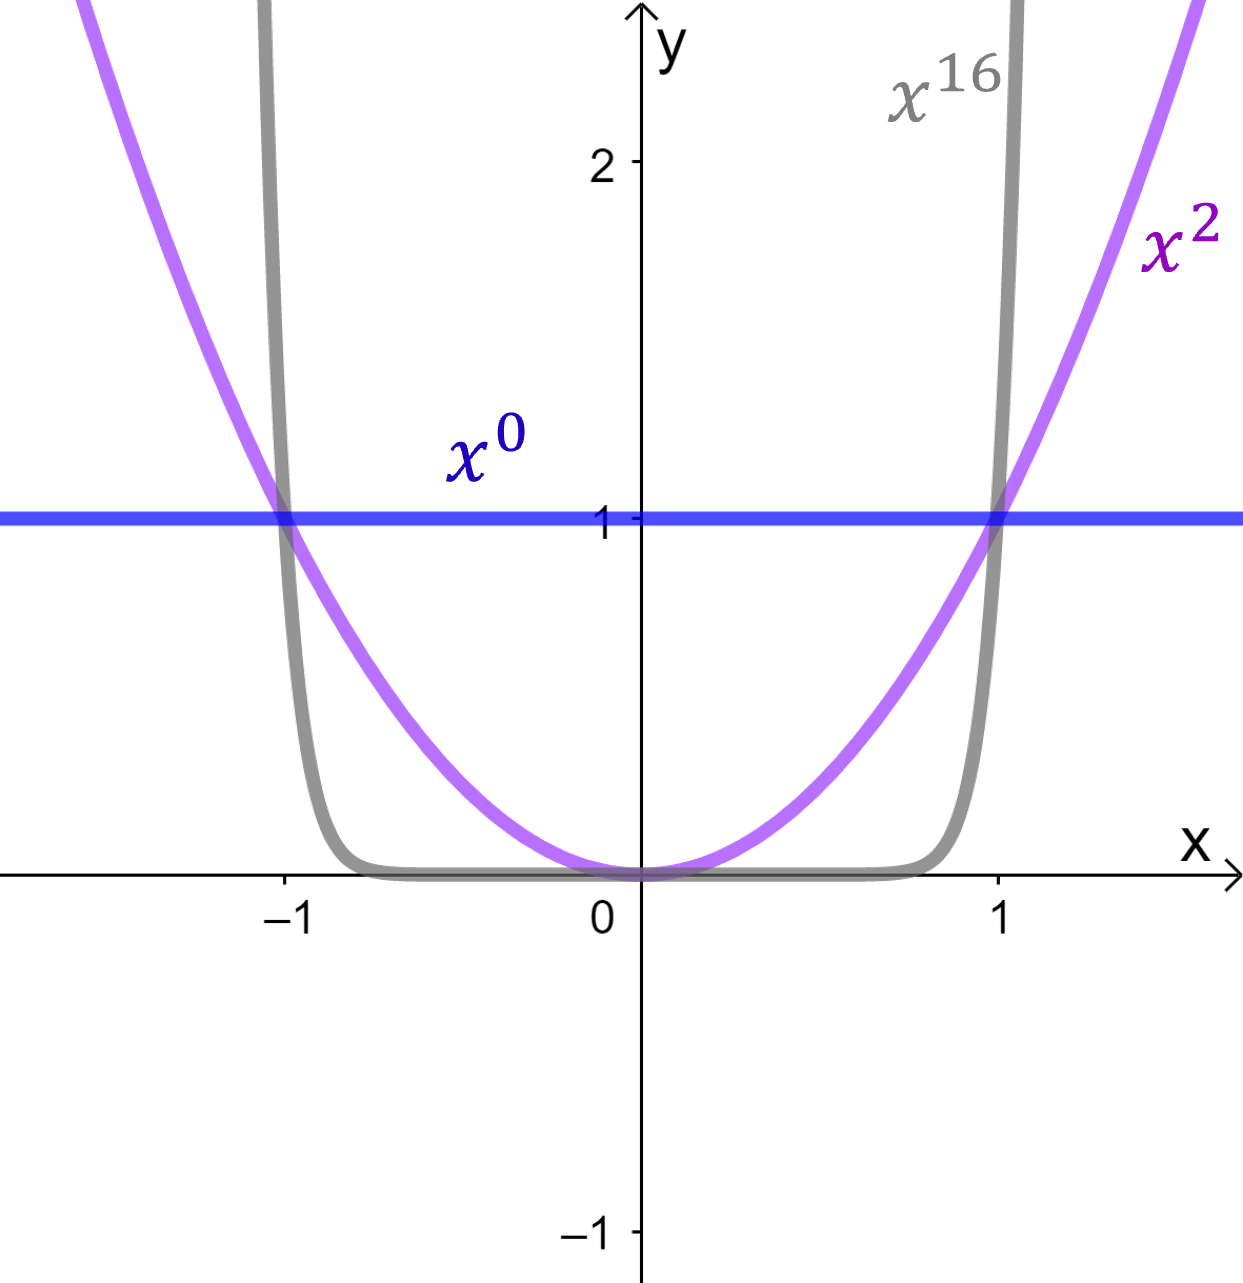
\includegraphics[width=\textwidth]{../Mathematik_1/Bilder/potenzfunktionen_gerade_exponenten.png}
	\end{minipage}
	\begin{minipage}{0.5\textwidth}
		Potenzfunktionen \[ f: \mathbb R \to [0, \infty), x\mapsto x^{2n}, \, n\in \mathbb N^+\] mit geradem Exponenten sind\ldots  
	\begin{itemize}
		\item achsensymmetrisch (gerade), also \[ f(x) = f(-x)\,,\] 
		\item auf $(-\infty, 0]$ streng monoton fallend,
		\item auf $[0,\infty)$ streng monoton steigend,
		\item auf \(\mathbb R\) \textcolor{blue}{nicht bijektiv} und damit nicht invertierbar!
	\end{itemize}
	\end{minipage}
\end{theorembox}

\begin{theorembox}{Monotonie und Symmetrie von Potenzfunktionen mit ungeradem Exponenten}{ }
	\begin{minipage}{0.35\textwidth}
	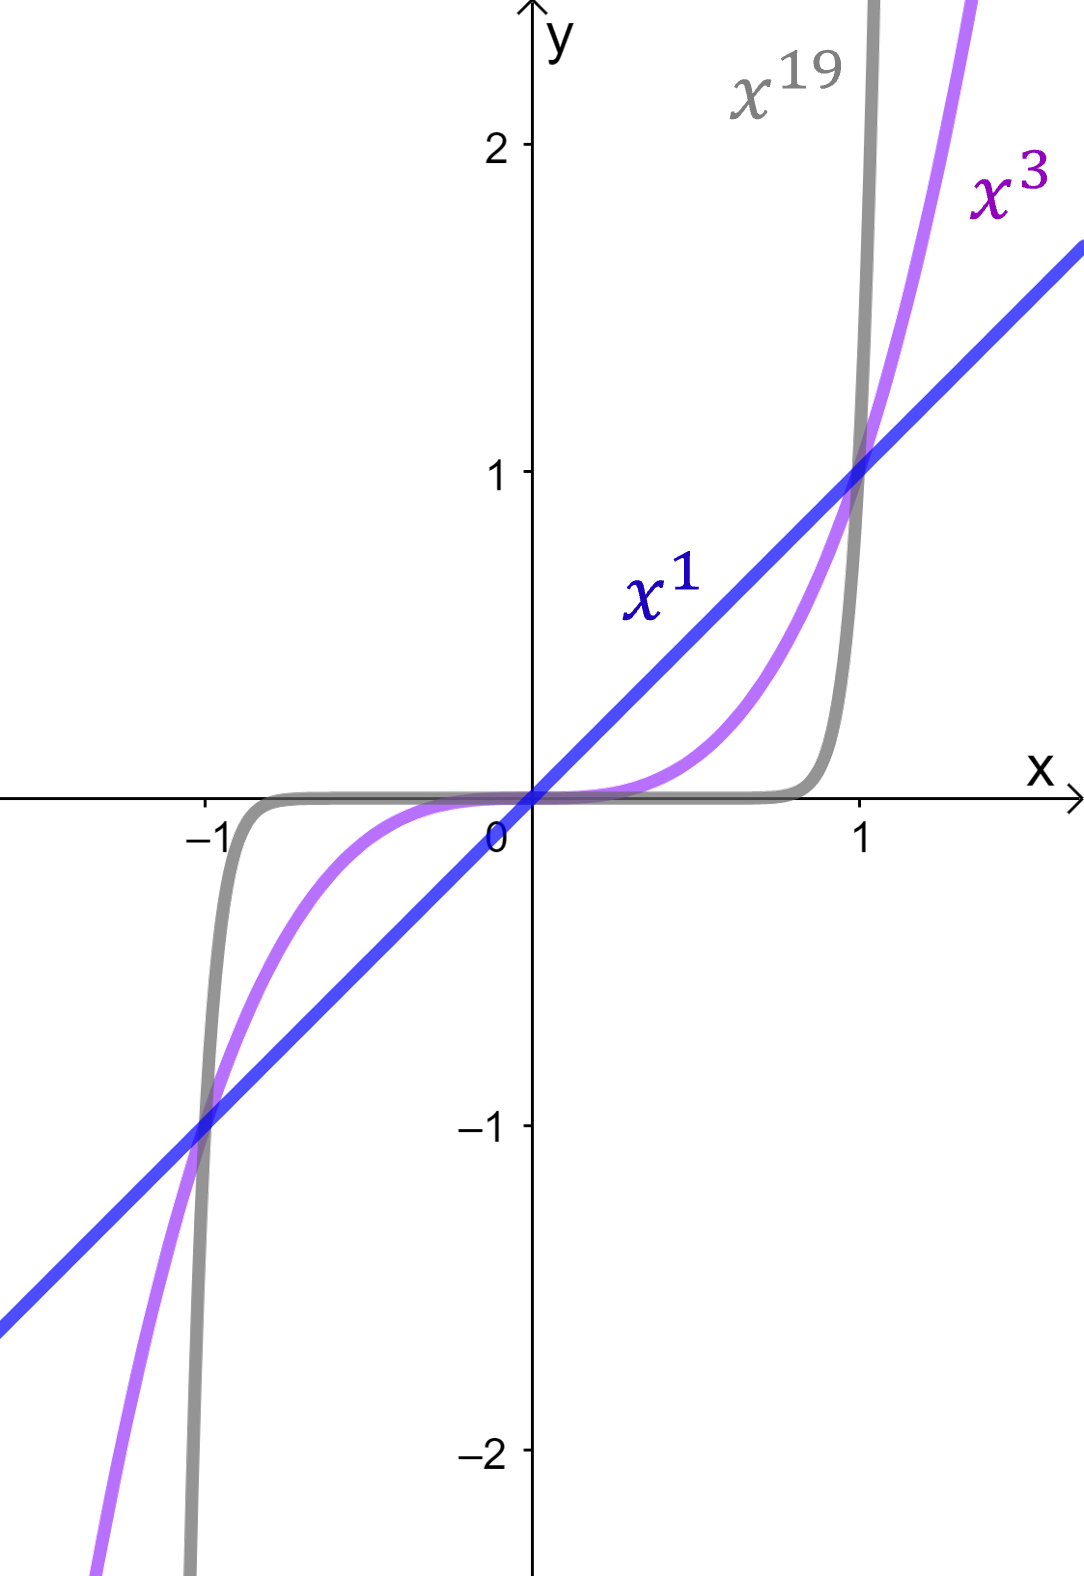
\includegraphics[width=\textwidth]{../Mathematik_1/Bilder/potenzfunktionen_ungerade_exponenten.png}
	\end{minipage}
	\begin{minipage}{0.5\textwidth}
		Potenzfunktionen \[f: \mathbb R\to \mathbb R,  x\mapsto x^{2n-1}, \, n\in \mathbb N^+\] mit ungeradem Exponenten sind \ldots
	\begin{itemize}
		\item punktsymmetrisch (ungerade), also \[f(-x) = -f(x)\,,\] 
		\item auf \(\mathbb R\) streng monoton steigend, 
		\item auf \(\mathbb R\) bijektiv und damit invertierbar.
	\end{itemize}
	\end{minipage}
\end{theorembox}

\subsection{Wurzelfunktionen}

Die Monotonie- und Injektivit�tseigenschaften der Potenzfunktionen bestimmen unmittelbar, ob und auf welchem Definitionsbereich sie umgekehrt werden k�nnen. Ihre Umkehrfunktionen f�hren zu den Wurzelfunktionen (\emph{root functions}).

Ungeradzahlige Wurzeln sind die \underline{Umkehrfunktionen}\randverweis{MA1-eigenschaften-von-funktionen} der entsprechenden Potenzfunktionen. 
\begin{exabox}{Ungeradzahlige Wurzeln}{ }

  \begin{minipage}{0.4\textwidth}
	  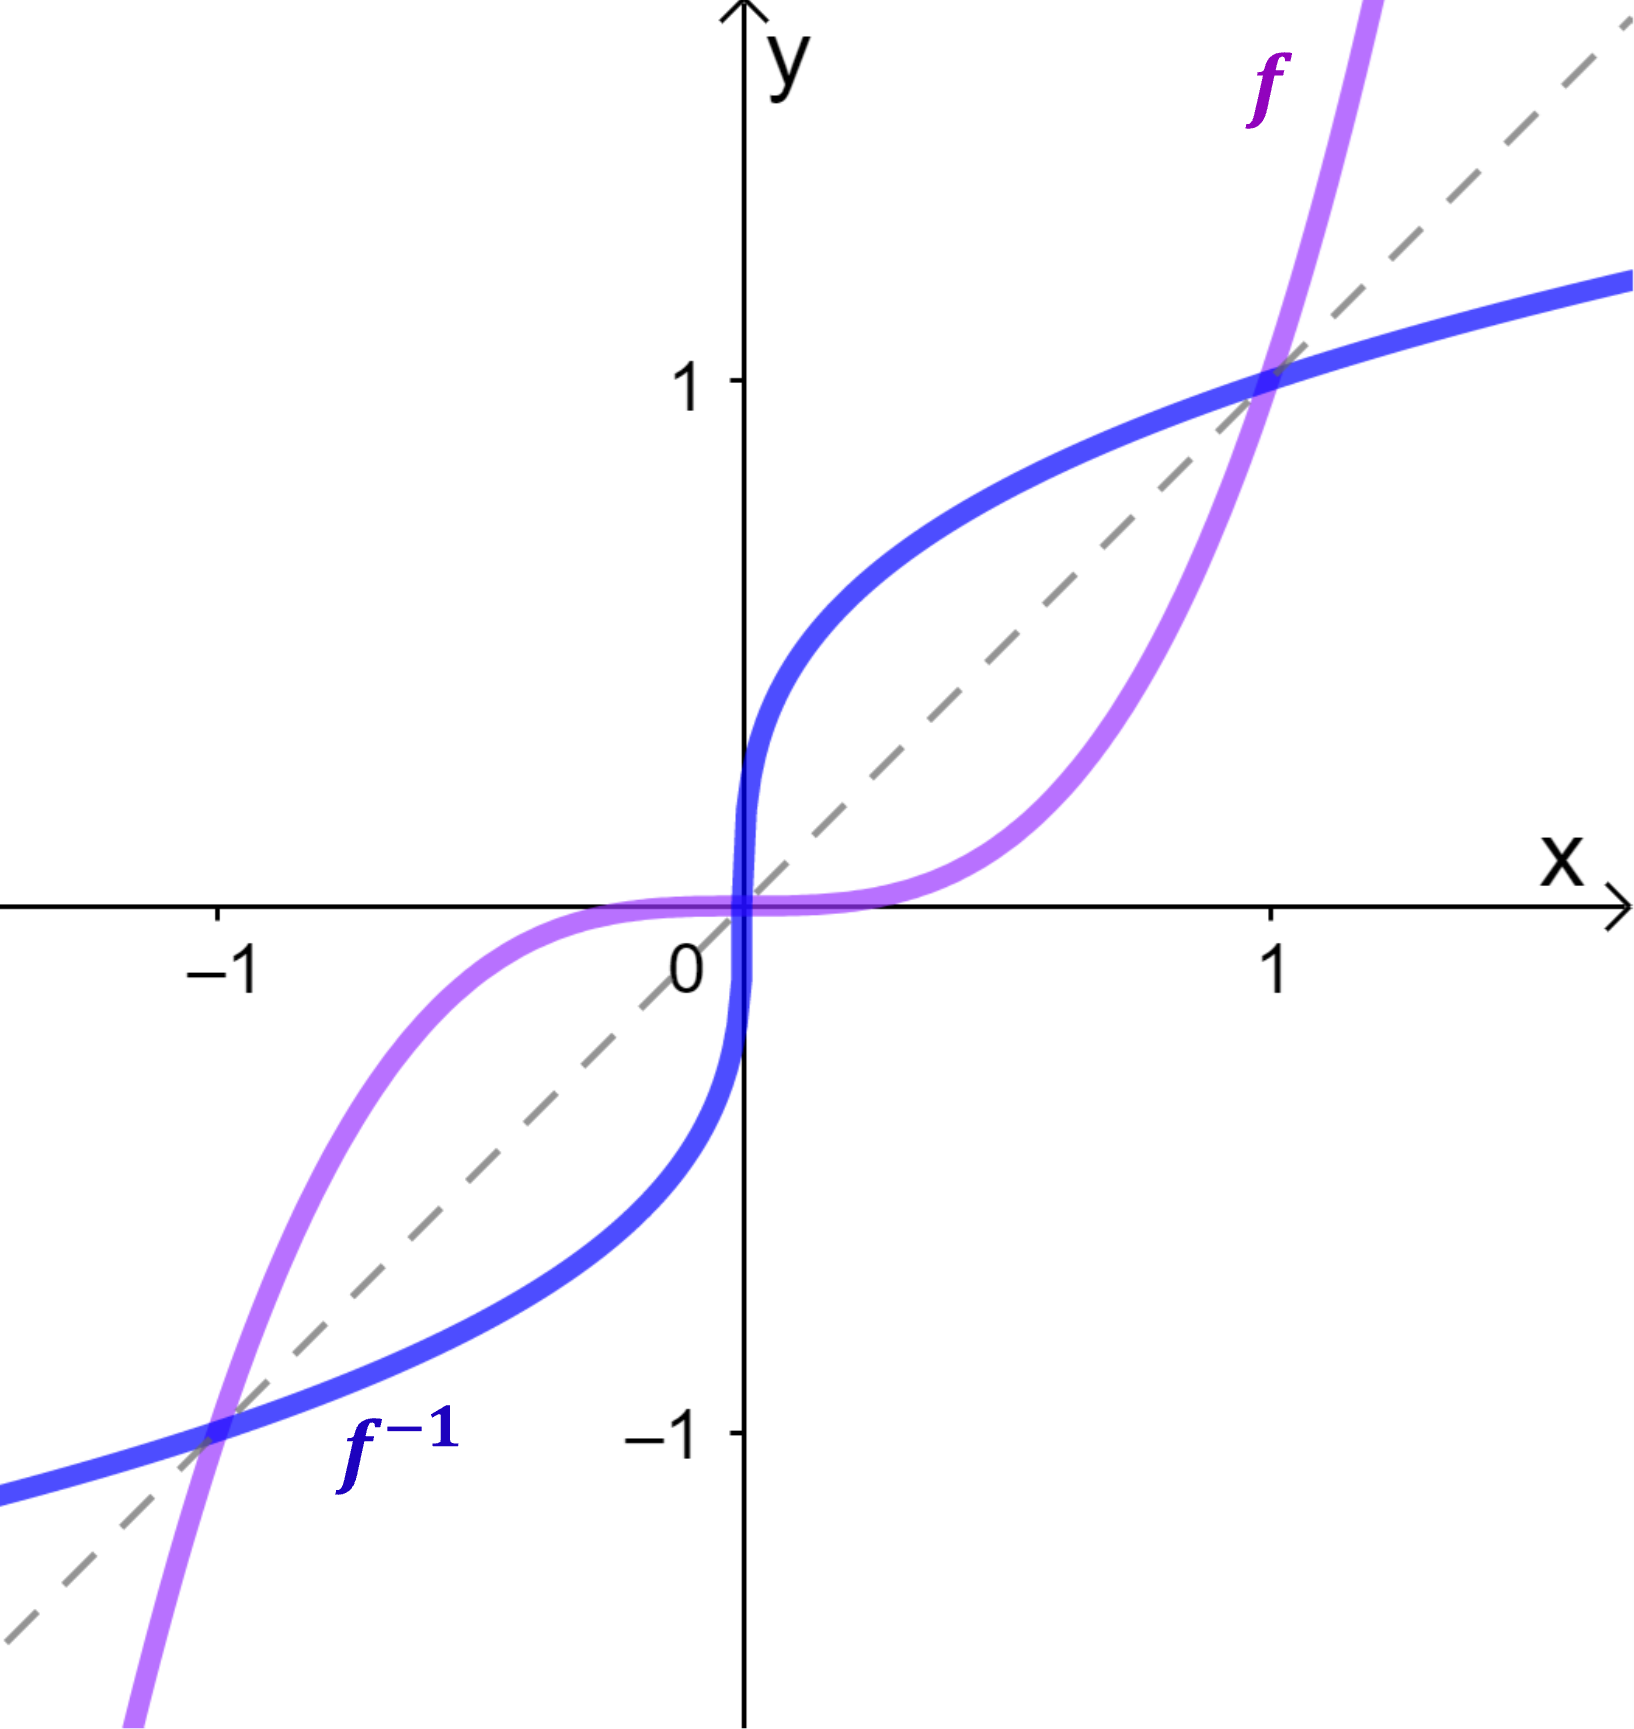
\includegraphics[width=\textwidth]{../Mathematik_1/Bilder/wurzelfunktionen_potenz_drei_dritte_wurzel.png}
\end{minipage}
\begin{minipage}{0.5\textwidth}
	\begin{itemize}
		\item \(f: x\mapsto x^3\) ist auf \(\mathbb R\) eine Potenzfunktion mit ungeradem Exponenten. 
		\item Da \(f\) auf \(\mathbb R\) streng monoton steigend und damit injektiv ist, besitzt sie auf ganz \(\mathbb R\) eine Umkehrfunktion.
		\item \(f^{-1}: x\mapsto \sqrt[3]{x}\) ist die Umkehrfunktion.
		\item "\,\textcolor{blue}{Umkehrfunktion}"\, und \textcolor{violett}{Funktion} sind an der Winkelhalbierenden gespiegelt.
		\item Ungeradzahlige Wurzeln sind f�r alle reellen Zahlen definiert. F�r negative Argumente liefern sie negative Ergebnisse.
	\end{itemize}
\end{minipage}
\end{exabox}

Potenzfunktionen mit geradem Exponenten sind auf \(\mathbb R\) nicht injektiv und besitzen daher dort keine Umkehrfunktion. Auf dem eingeschr�nkten Definitionsbereich \([0,\infty)\) sind sie dagegen streng monoton steigend und damit bijektiv auf \([0,\infty)\).

\begin{exabox}{Geradzahlige Wurzeln}{ }
  \begin{minipage}{0.4\textwidth}
	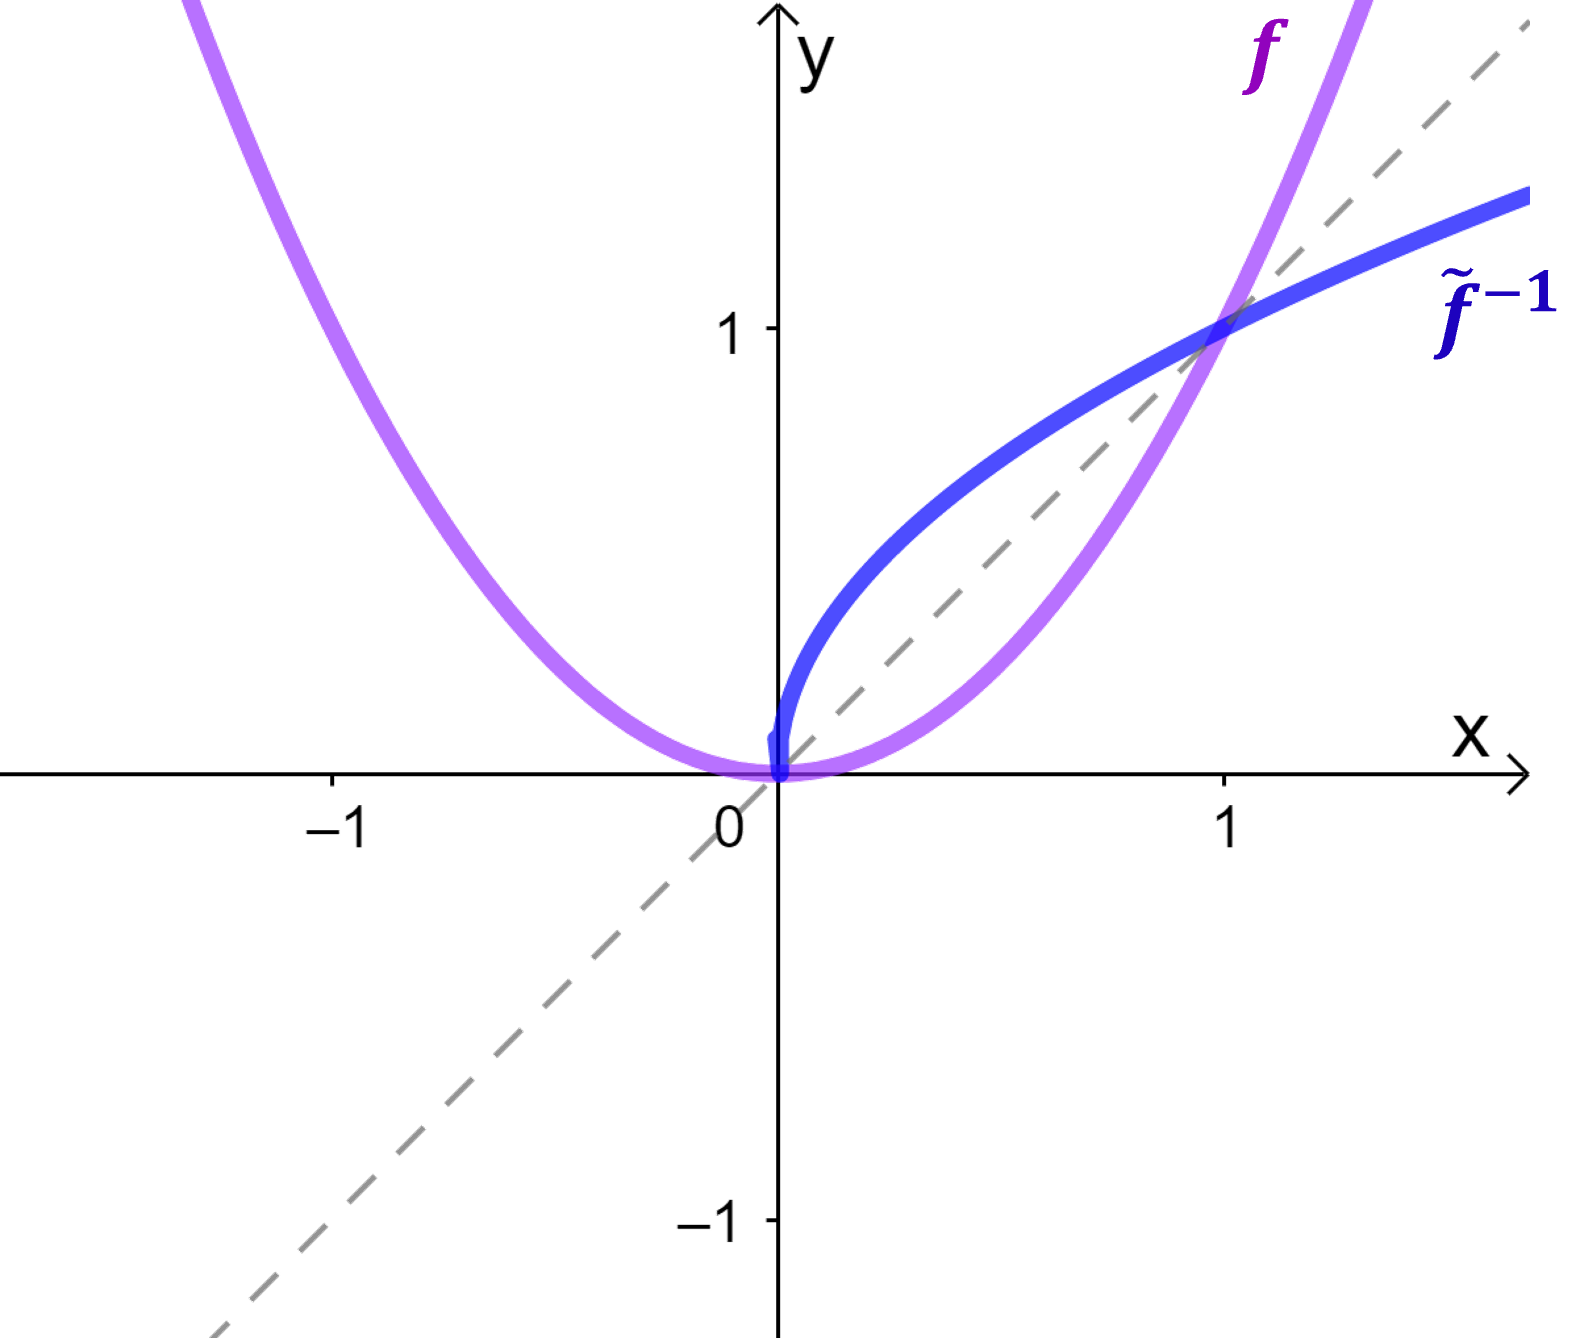
\includegraphics[width=\textwidth]{../Mathematik_1/Bilder/wurzelfunktionen_quadratfunktion_quadratwurzel.png}
\end{minipage}
\begin{minipage}{0.5\textwidth}
	\begin{itemize}
		\item \(f: \mathbb R \to [0,\infty), x\mapsto x^4\) ist auf \(\mathbb R\) eine Potenzfunktion mit geradem Exponenten. 
		\item \(f\) ist auf \(\mathbb R\) nicht invertierbar.
		\item \(\tilde f: [0,\infty) \to [0,\infty), x\mapsto x^4\) ist bijektiv und damit invertierbar.
		\item \(\tilde f^{-1}: x\mapsto \sqrt[4]{x}\) kehrt die Potenzfunktion auf \( [0,\infty)\) um.
		\item "\,\textcolor{blue}{Umkehrfunktion}"\, und \textcolor{violett}{Funktion} sind an der Winkelhalbierenden gespiegelt.

		\item Geradzahlige Wurzeln sind im Reellen nur f�r nichtnegative Argumente definiert und liefern ausschlie�liche nichtnegative Ergebnisse.
	\end{itemize}
\end{minipage}
\end{exabox}

Potenzfunktionen und Wurzelfunktionen treten h�ufig in Gleichungen auf. F�r Gleichungen der Form
\[
x^n=c
\]
h�ngt die Anzahl der reellen L�sungen entscheidend davon ab, ob der Exponent \(n\) gerade oder ungerade ist. \marginpar{Aufgaben} 

\begin{theorembox}{Gleichungen mit Potenzfunktionen}{ }
	Es sei $n\in \mathbb N^+$. Gesucht sind alle \textbf{reellen} L�sungen $x\in \mathbb R$ der Gleichung  \[ x^n = c\,.\]
	F�r $n$ gerade, also $n=2,4,6,\cdots$ besitzt die Gleichung 
	\begin{itemize}
		\item f�r $c>0$ die beiden L�sungen $x_1= - \sqrt[n]{c}$,  $x_2= \sqrt[n]{c}$,
		\item f�r $c=0$ die L�sung $x=0$, 
		\item f�r $c<0$ keine L�sung. 
	\end{itemize}
	F�r $n$ ungerade, also $n=1,3,5,7,\cdots$ besitzt die Gleichung 
	\begin{itemize}
		\item f�r $c\geq0$ die L�sung $x= \sqrt[n]{c}$,
		\item f�r $c<0$ die L�sung  $x=-\sqrt[n]{|c|}$.
	\end{itemize}
\end{theorembox}

\begin{exabox}{Gleichungen mit Potenzen}{ }

	\begin{itemize}
		\item F�r die Gleichung \(x^4=16\) ist der Exponent gerade und die rechte Seite positiv. Daher gibt es zwei reelle L�sungen:
\[
x=-\sqrt[4]{16}=-2
\qquad\text{oder}\qquad
x=\sqrt[4]{16}=2.
\]
Die L�sungsmenge ist also \( \mathbb L=\{-2,2\}\).

\item Die Gleichung \(x^3=-8 \) besitzt wegen des ungeraden Exponenten genau eine reelle L�sung:
\[
x=\sqrt[3]{-8}=-2.
\]
Damit gilt \( \mathbb L=\{-2\} \).
\end{itemize}

\end{exabox}

%Es gibt verschiedene Meinungen dazu, ob man ungerade Wurzeln aus negativen Zahlen ziehen darf oder ob doch lieber alle Wurzeln nur f�r reelle Zahlen ab $0$ aufw�rts definiert sein sollten. Mit Wolfram Alpha gibt es noch eine gr��ere �berraschung: \verb+cubic root of -8+ wird dort eine komplexe Zahl - aus gutem Grund (Hauptwert der Wurzel). 

\subsection{Verallgemeinerung der Potenzrechenregeln}

F�r das Produkt positiver ganzzahliger Potenzen $a^n$ und $a^m$ derselben Zahl $a\in \mathbb R$ gilt offensichtlich: $$a^n \cdot a^m = a^{n+m}\,.$$

Die bekannten Potenzrechenregeln sollen auch f�r allgemeinere Exponenten gelten. Dadurch ergibt sich auf nat�rliche Weise, wie Potenzen mit dem Exponenten \(0\), mit negativen ganzzahligen Exponenten und schlie�lich mit gebrochenzahligen Exponenten definiert werden m�ssen.

Damit die Potenzregel auch f�r den Exponenten \(0\) und f�r negative
ganzzahlige Exponenten erhalten bleibt, definiert man f�r \(a\neq0\)
\[
a^0:=1,
\qquad
a^{-n}:=\frac{1}{a^n},
\qquad n\in\mathbb N^+.
\]

F�r eine positive ganzzahlige Potenz $(a^n)^m$ einer positiven ganzzahligen Potenz $a^n$ einer Zahl $a \in (0,\infty)$ gilt offensichtlich:
  $$(a^n)^m = a^{n\cdot m}\,.$$

Um  diese  Regel  auf  gebrochenzahlige  Exponenten  zu  erweitern,  muss man definieren:
$$a^{\frac1n}: = \sqrt[n]{a}, \quad n\in\mathbb N^+\,.$$

Fassen wir die Rechenregeln zusammen:\marginpar{Aufgaben}

\begin{theorembox}{Rechenregeln}{ }
F�r \(a,b>0\) und rationale Exponenten \(r,s\in\mathbb Q\) gelten
\begin{align*}
(a\cdot b)^r &= a^r\cdot b^r,\\
a^r\cdot a^s &= a^{r+s},\\
(a^r)^s &= a^{rs},\\
a^{-r} &= \frac{1}{a^r}.
\end{align*}

Ein rationaler Exponent
\[
r=\frac{m}{n},
\qquad
m\in\mathbb Z,\quad n\in\mathbb N^+,
\]
wird dabei durch
\[
a^{\frac{m}{n}}
:=
\sqrt[n]{a^m}
=
\left(\sqrt[n]{a}\right)^m
\]
definiert.
\end{theorembox}


Bei der Basis \(0\) und insbesondere bei negativen Basen m�ssen die Voraussetzungen der Potenzrechenregeln sorgf�ltig beachtet werden.

\begin{exabox}{Vorsicht bei negativen Basen}{ }

	F�r \(x\geq0\) gilt \(\sqrt{x^2}=x\). F�r beliebige \(x\in\mathbb R\) muss dagegen ber�cksichtigt werden, dass die Quadratwurzel stets nichtnegativ ist. Daher gilt allgemein \( \sqrt{x^2}=|x|\).

Beispielsweise ist
\[
\sqrt{(-3)^2}
=
\sqrt9
=
3
=
|-3|
\neq -3.
\]

Die Potenzregel \( (a^n)^m=a^{nm} \) kann daher bei negativen Basen und nichtganzzahligen Exponenten nicht ohne zus�tzliche Voraussetzungen angewendet werden.

\end{exabox}
 \newpage % Potenzfunktionen und Wurzelfunktionen
\setcounter{exercise}{0} \ifintegriereaufgaben
\section*{Potenz- und Wurzelfunktionen Aufgaben}\label{MA1-potenz-und-wurzelfunktionen-aufgaben}
	
	Regeln und Beispiele, die zur Bearbeitung der Aufgaben hilfreich sind, finden Sie im Skript\wennreferenzvorhanden{MA1-potenz-und-wurzelfunktionen}{ (Abschnitt \abschnittsverweis{MA1-potenz-und-wurzelfunktionen})} und, falls Sie nicht weiterkommen, schauen Sie \hyperref[MA1-potenz-und-wurzelfunktionen-loesungen]{hier}.
\else 
\section{Potenz- und Wurzelfunktionen Aufgaben}\label{MA1-potenz-und-wurzelfunktionen-aufgaben}
	
	Regeln und Beispiele, die zur Bearbeitung der Aufgaben hilfreich sind, finden Sie im Skript und, falls Sie nicht weiterkommen, schauen Sie \hyperref[MA1-potenz-und-wurzelfunktionen-loesungen]{hier}.
\fi 

\begin{exercisebox}[$f:x\mapsto  3\sqrt{4-x^2}$]
  Gegeben ist die Funktion $f:x\mapsto  3\cdot \sqrt{4-x^2}$.
  \begin{itemize}
	  \item[(a)] Geben Sie die Funktionswerte an den Stellen $-1$ und $\sqrt{3}$ an.
    \item[(b)] Berechnen Sie $f(0)$, $f(2)$, und $f(\frac23)$.
    \item[(c)] Bestimmen Sie die maximale Definitionsmenge und die Wertemenge von $f$.
    \item[(d)] Pr�fen Sie rechnerisch, ob der Punkt $P(-\sqrt 2| 3\sqrt 2)$ auf dem Graphen von $f$ liegt.
  \end{itemize}
\end{exercisebox}

\begin{exercisebox}[Symmetrie]
	Bestimmen Sie das Symmetrieverhalten der folgenden Funktionen in ihrem maximalen Definitionsbereich
  \begin{eqnarray*}
	  \begin{array}{lll} 
		  (a)\, f:x\mapsto 4\cdot x^2-16 &\quad (b)\, f:x\mapsto \displaystyle{\frac{x^3}{x^2+1}} &\quad (c)\; f:x\mapsto |x^2-4|\\ (d)\; f:x\mapsto \displaystyle{\frac{x^2-1}{1+x^2}} &\quad (e)\, f:x\mapsto \sqrt{x^2-25} &\quad (f)\,f:x\mapsto \displaystyle{\frac{1}{x-1}}
	  \end{array}
  \end{eqnarray*}
\end{exercisebox}

\begin{exercisebox}[Monotonie]
	Untersuchen Sie die folgenden Funktionen auf Monotonie. Hinweis: Benutzen Sie die bekannten Symmetrieeigenschaften der Potenz- und Wurzelfunktionen.
  \begin{eqnarray*}
	  \begin{array}{llll} 
		  (a)\, f:x\mapsto x^4 &\quad (b)\; f:x\mapsto \displaystyle{\sqrt{x-1}} &\quad (c)\; f:x\mapsto x^3+2\cdot x \quad (d)\; f:x\mapsto \displaystyle{| x^2-2\cdot x+1|} 
	  \end{array}
  \end{eqnarray*}
\end{exercisebox}

\begin{exercisebox}[Umkehrfunktion]
  \begin{itemize}
	  \item[(a)] Welche der Potenzfunktionen $f$ mit $f(x) = x^n,\; n\in\mathbb N\setminus\{0\}$  sind umkehrbar?
	  \item[(b)] Wie lauten die Umkehrfunktionen von folgenden Funktionen? \[ (a) \; f:x\mapsto \frac{1}{2\cdot x}\quad \quad (b)\; g:x\mapsto \sqrt{3\cdot x}\]
  \end{itemize}
\end{exercisebox}

\begin{exercisebox}[Gleichungen]
	L�sen Sie folgenden Gleichungen
  \begin{eqnarray*}
	  \begin{array}{llll} 
		  (a)\, \sqrt{ -3 +2\cdot x} = 2 &\quad (b)\; \sqrt{x^2+4}-x = -2 &\quad (c)\; \sqrt{x-1} = \sqrt{x+1}\quad& (d)\; \sqrt{2\cdot x^2-1}+x=0 
	  \end{array}
  \end{eqnarray*}
\end{exercisebox}

\begin{exercisebox}[Gleichungen]
	\begin{enumerate}
		\item[(a)] Bestimmen Sie alle L�sungen der Gleichung \[ -2\cdot x^2+6 = 4\cdot x \]
		\item[(b)] F�r welchen Parameter $p$ hat die folgende Gleichung genau eine L�sung? \[ x^2 + p\cdot x+3 \cdot p = 0\]
		\item[(c)] F�r welche Werte von $c$ hat die folgende Gleichung keine reelle L�sung? \[ x^2 + 2\cdot c \cdot x+c = 0\]
  \end{enumerate}
\end{exercisebox}
 \newpage 
\setcounter{satz}{0} \setcounter{def}{0} \setcounter{exa}{0}  \section{Polynome}\label{MA1-polynome}

\begin{table}[H]
  \centering
  \begin{tabularx}{\textwidth}{p{0.9\textwidth} p{0.1\textwidth}}
    \toprule
	  \multicolumn{2}{c}{\textbf{�bersicht �ber Lernziele und Voraussetzungen}}\\
    \midrule
	  \textbf{Lernziele} &\\[.5\normalbaselineskip]
	  \tabitem Polynome definieren und ihren Grad bestimmen &\\
\tabitem das asymptotische Verhalten eines Polynoms aus Grad und f�hrendem Koeffizienten beschreiben &\\
\tabitem eine Polynomdivision durchf�hren &\\
\tabitem den Zusammenhang zwischen Nullstellen und Linearfaktoren erkl�ren und Polynome faktorisieren &\\
\tabitem die Vielfachheit einer Nullstelle am Verhalten des Funktionsgraphen interpretieren &\\
\tabitem quadratische Funktionen in Koeffizientenform, Scheitelpunktform und Linearfaktorzerlegung darstellen und die jeweils unmittelbar erkennbaren Eigenschaften interpretieren &\\
\tabitem die Abbildungsvorschrift eines Polynoms aus gegebenen Eigenschaften konstruieren &\\
    \midrule
	  \textbf{Voraussetzungen} \\[.5\normalbaselineskip]
	  \tabitem Grundlagen & \abschnittsverweis{MA1-mengen-und-logik}-\abschnittsverweis{MA1-aequivalenzumformungen}\\
	  \tabitem Potenzfunktionen und Wurzelfunktionen  & \abschnittsverweis{MA1-potenz-und-wurzelfunktionen}\\
    \bottomrule
  \end{tabularx}
\end{table}

\ifintegriereaufgaben \noindent �bungsaufgaben zum Thema finden Sie hier: \hyperref[MA1-polynome-aufgaben]{Aufgaben}
\vspace{0.3cm}
\hrule
 \fi

\subsection{Was ist ein Polynom?}

Eine Funktion
\[
p:\mathbb R\to\mathbb R
\]
hei�t \textbf{Polynom} (\emph{polynomial}), wenn ihre Abbildungsvorschrift die Form
\[
p(x)
=
a_n\cdot x^n+a_{n-1}\cdot x^{n-1}+\dots+a_1\cdot x+a_0
\]
mit
\[
a_0,\dots,a_n\in\mathbb R
\]
besitzt.

Ist \(a_n\neq0\), so hei�t \(n\) der \textbf{Grad} (\emph{degree}) des Polynoms. Die Zahlen
\[
a_0,\dots,a_n
\]
hei�en seine \textbf{Koeffizienten} (\emph{coefficients}).

Neben dem Grad sind insbesondere das asymptotische Verhalten und die
Nullstellen eines Polynoms von Bedeutung. Unter dem asymptotischen Verhalten
wird der typische Verlauf des Funktionsgraphen f�r betragsm��ig gro�e \(x\)
verstanden. Die Nullstellen eines Polynoms sind diejenigen \(x\in\mathbb R\),
f�r die \(p(x) = 0\) gilt.

Ist \(p\) von ungeradem Grad, so besitzt \(p\) mindestens eine reelle
Nullstelle. Anschaulich folgt dies daraus, dass die beiden Enden des
Funktionsgraphen f�r \(x\to-\infty\) und \(x\to\infty\) in entgegengesetzte
Richtungen verlaufen. Eine pr�zise Begr�ndung dieser Aussage wird sp�ter
mithilfe der Stetigkeit m�glich.

\begin{exabox}{Verhalten von Polynomen}{ }
	\begin{minipage}{0.4\textwidth}
		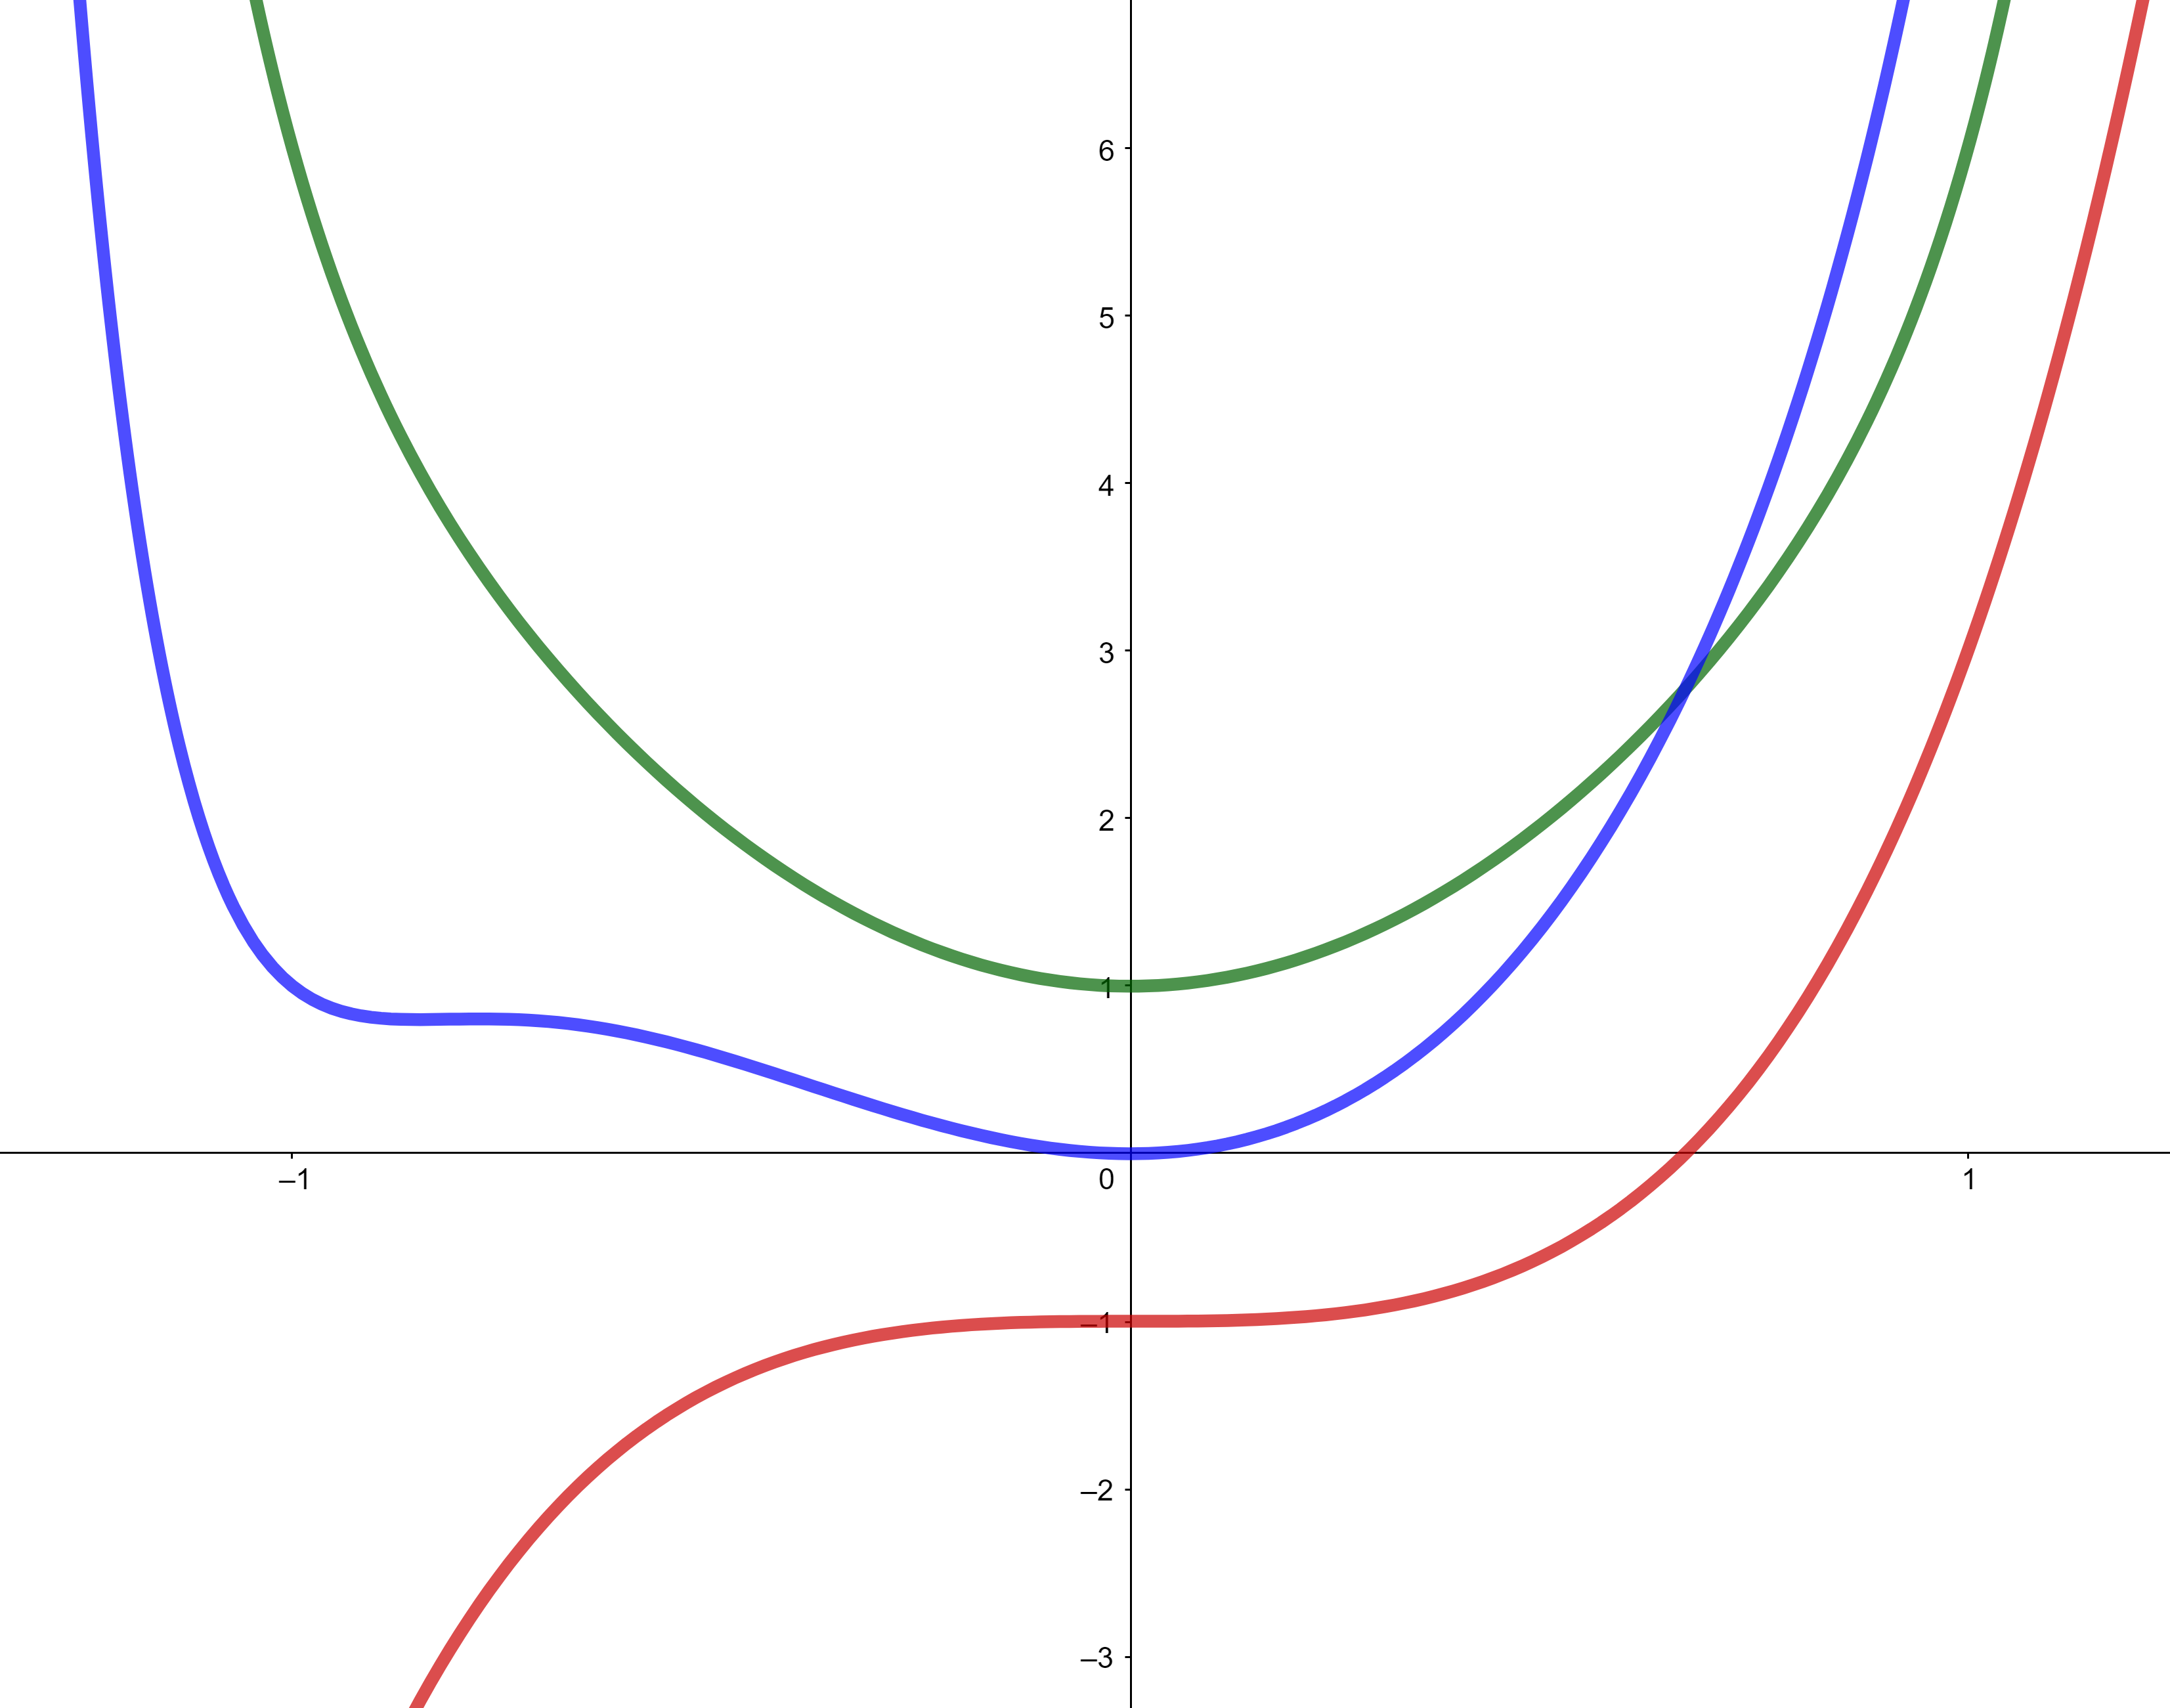
\includegraphics[width=\textwidth]{../Mathematik_1/Bilder/polynome_graphen_gerader_ungerader_grad.png}
\end{minipage}
\begin{minipage}{0.6\textwidth}
	Die Graphen links geh�ren zu folgenden Polynomen:
		\begin{itemize}
			\item \(\color{darkgreen}{h: x\mapsto x^{10}+4\cdot x^2+1}\)
			\item \(\color{red}{f: x\mapsto x^{5} +3\cdot x^3-1}\)
			\item \(\color{blue}{g: x\mapsto x^{10}+x^5+3\cdot x^3+4\cdot x^2}\)
		\end{itemize}
\end{minipage}
\end{exabox}

\noindent\textbf{Bemerkungen:}
\begin{itemize}
	\item Mit Polynomen lassen sich andere Funktionen approximieren. Die Exponentialfunktion und die trigonometrischen Funktionen k�nnen beispielsweise gut durch \underline{Polynome gen�hert werden}\randverweis{MA2-taylorreihen}:
  \begin{eqnarray*}
    e^x &\approx& 1 + x + \frac12\cdot x^2 + \frac{1}{3!}\cdot x^3 + \frac{1}{4!}\cdot x^4\,,\\
    \sin(x) &\approx& x - \frac{1}{3!}\cdot x^3\,,  \\
    \cos(x) &\approx& 1 - \frac12 \cdot x^2 + \frac{1}{4!}\cdot x^4 \,.
  \end{eqnarray*}
\item Polynome sind au�erdem beliebt als Hilfsmittel, um Messwerte zu interpolieren, beispielsweise mit einem \underline{linearen Spline}\randverweis{MA1-lineare-funktionen} oder auch mit Polynomen h�heren Grades.
	\begin{exabox}{Polynomiale Interpolation}{ }
	\begin{minipage}{0.4\textwidth}
	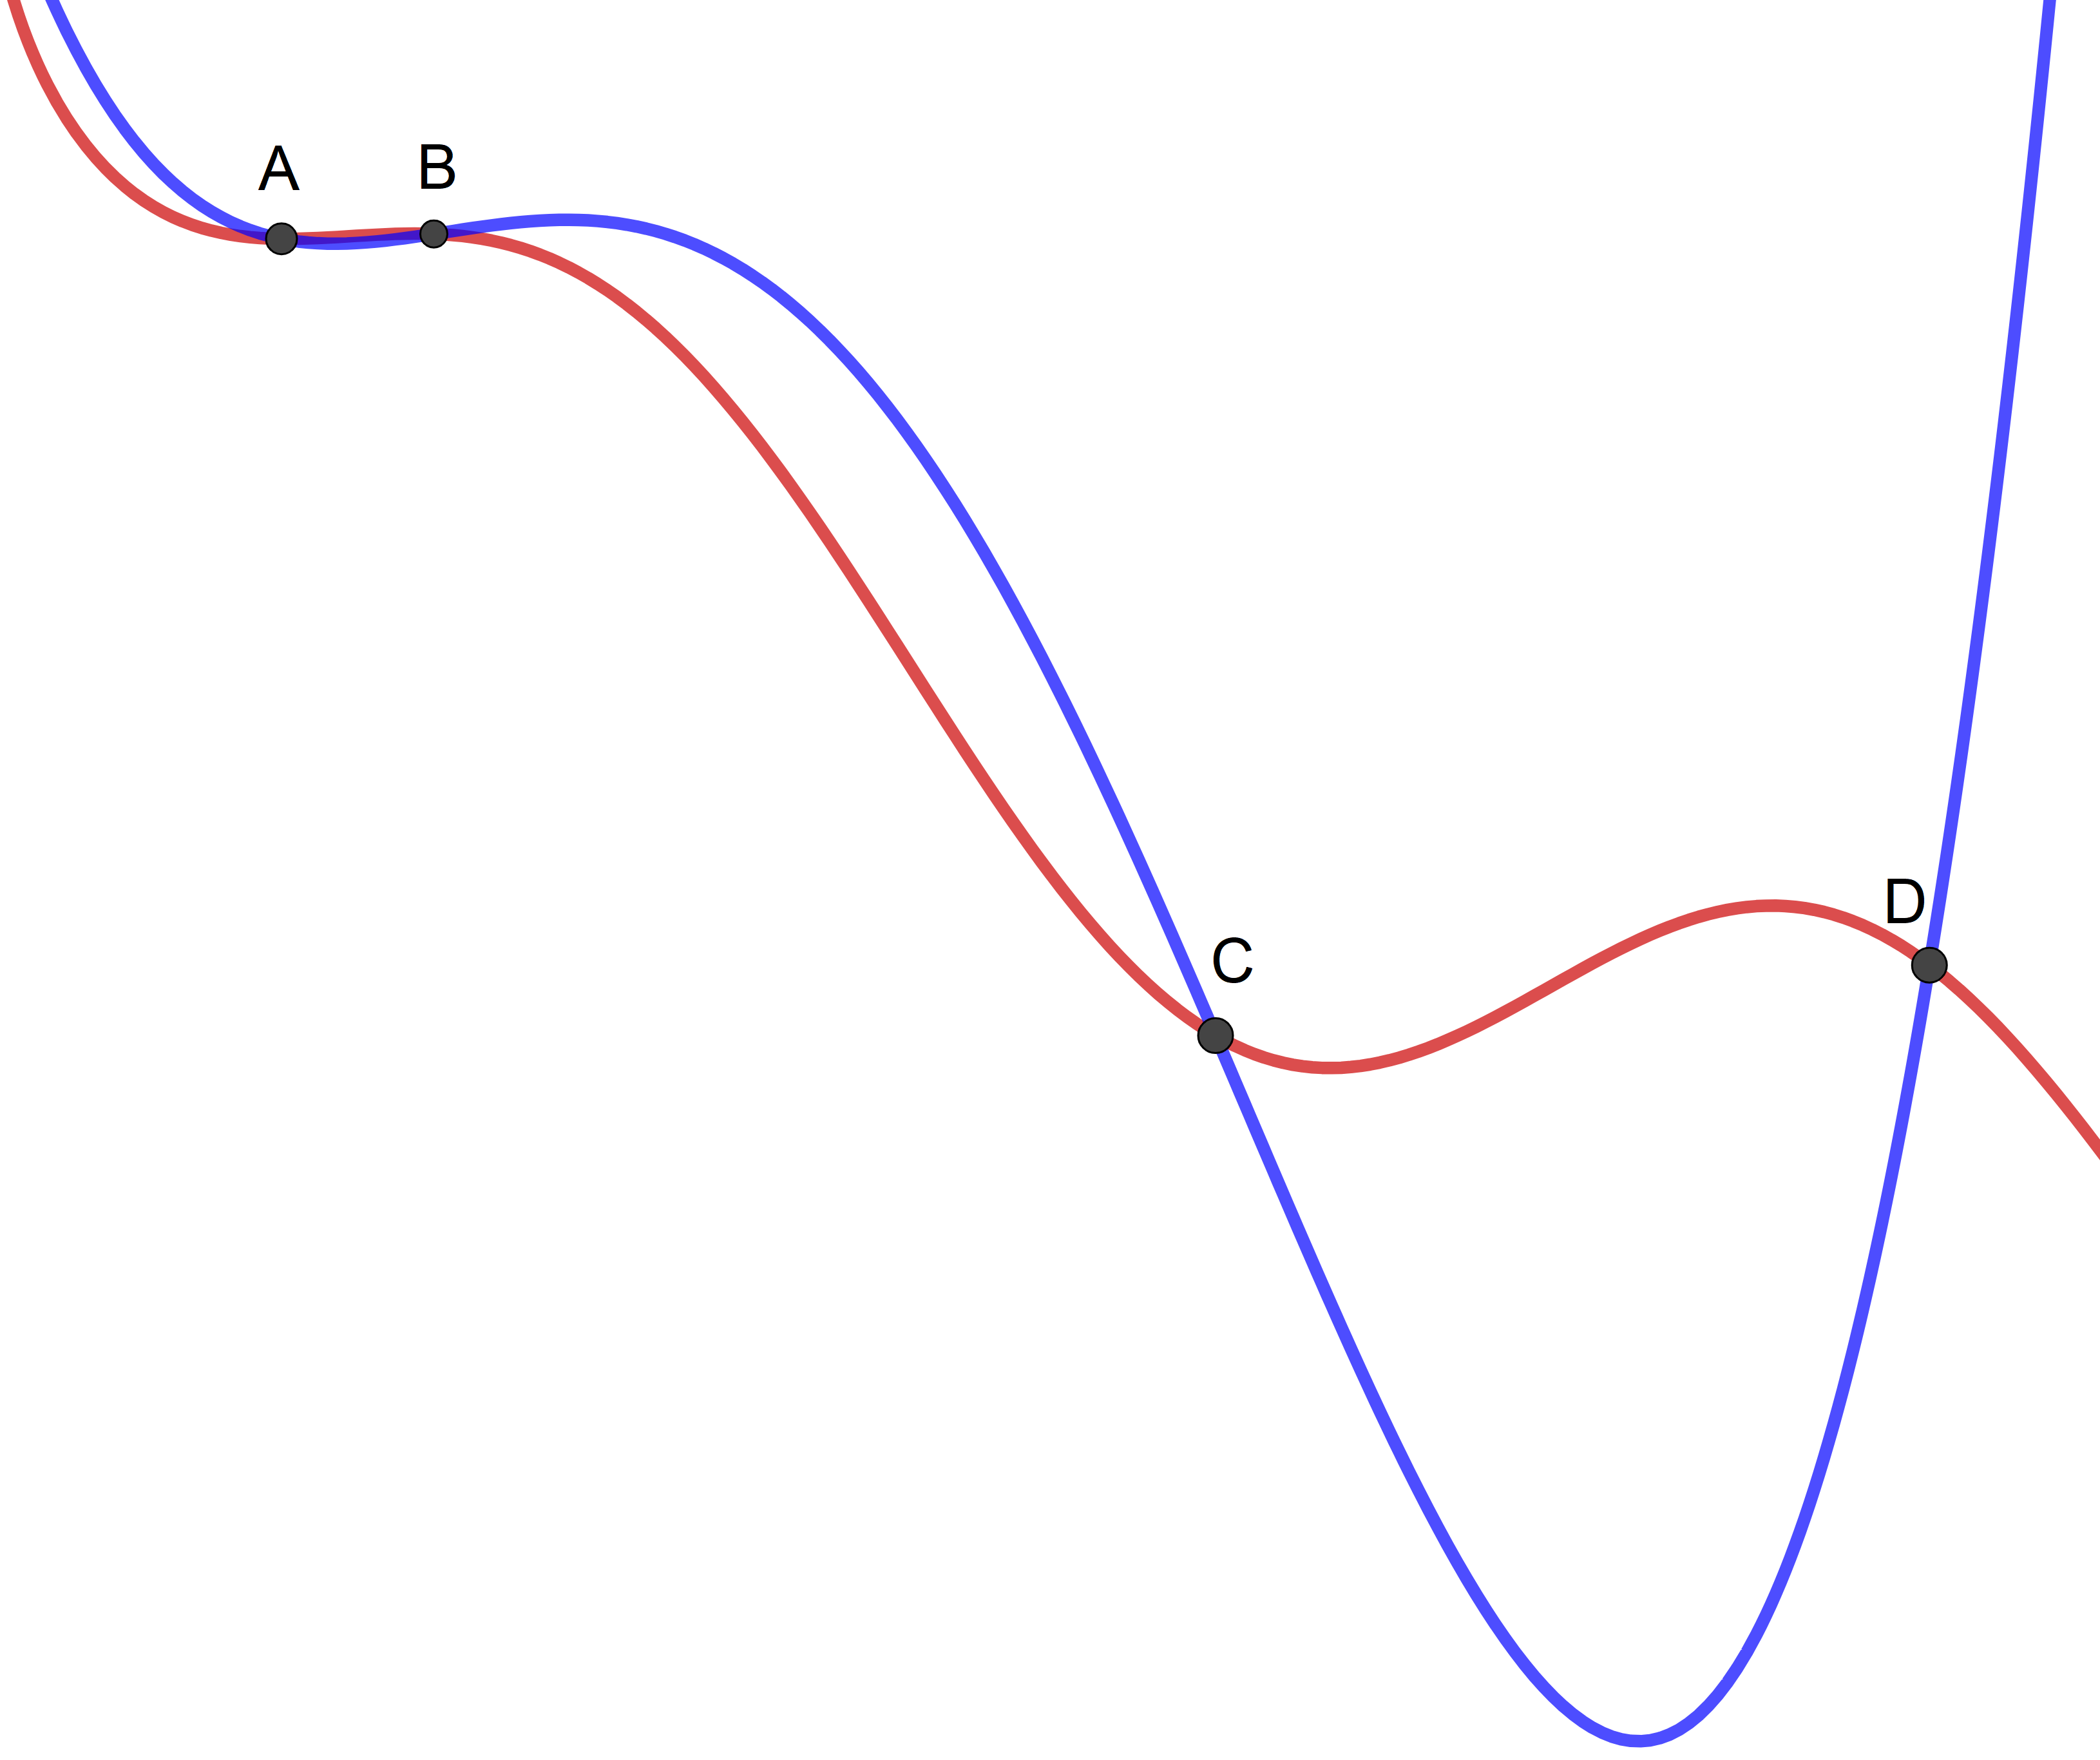
\includegraphics[width=\textwidth]{../Mathematik_1/Bilder/polynome_interpolation_funktionsvergleich.png}
\end{minipage}
\begin{minipage}{0.6\textwidth}
	\[\begin{cases} f: D_f \to \mathbb R, \;& x\mapsto \sin^2(x) - \sqrt{3\cdot x}\\
	p: \mathbb R \to \mathbb R, \;& x\mapsto \dfrac{3}{20}\cdot x^4 - \dfrac{13}{10}\cdot x^3+\dfrac{33}{10}\cdot x^2-\dfrac{319}{100}\cdot x\end{cases}\]
	\begin{itemize}
		\item[\(\Rightarrow \)] \(f\) hat den  Definitionsbereich \(D_f = [0,\infty)\).
		\item[\(\Rightarrow \)] \(p\) ist ein Polynom vierten Grades, also \(D_p = \mathbb R\).
		\item[\(\Rightarrow \)] \(p\) interpoliert \(f\) an f�nf ausgew�hlten Punkten.
		\item[\(\Rightarrow \)] asymptotisch sind \(f\) und \(p\) komplett verschieden.
		\item[\(\Rightarrow \)] die Interpolation ist eine lokale Approximation.
	\end{itemize}
\end{minipage}
		\end{exabox}

	\item Daneben treten Polynome bei der Analyse von \underline{gew�hnlichen Differentialgleichungen}\randverweis{MA2-differentialgleichungen} auf.
%Gesucht sei beispielsweise eine Funktion $f$ mit $f''-5f'+6f \stackrel{!}{=}0$. Dann kann man einen L�sungsansatz der Form $f(x) = e^{\lambda x}$ mit $\lambda\in\mathbb R\setminus\{0\}$ machen und erh�lt durch ein Einsetzen der Ableitungen $(*)$ eine polynomiale Gleichung, die es zu L�sen gilt:
%\begin{exabox}{Charakteristisches Polynom}{ }
%  $ \left.\begin{array}{rcl}
%  f(x) &=& e^{\lambda x}\\
%  f'(x) &=& \lambda e^{\lambda x}\\
%  f''(x) &=& \lambda^2 e^{\lambda x}
%\end{array}\; \right\} \;\;  \stackrel{(*)}{\displaystyle{\Rightarrow}} \;
%  \lambda^2 e^{\lambda x} - \lambda e^{\lambda x} + 6 e^{\lambda x} \stackrel{!}{=} 0 \Leftrightarrow \lambda^2 - \lambda + 6 \stackrel{!}{=} 0\,.
%  $
%\end{exabox}

	\item Die \underline{Laplace-Transformation}\randverweis{MA2-systemanalyse} transformiert komplexe Systeme in den sogenannten Bildbereich, in dem es schlussendlich um die Analyse von Polynomen geht.
	\end{itemize}

\subsection{Polynomdivision}

Polynome kann man addieren, subtrahieren und multiplizieren und erh�lt wieder Polynome\randverweis{MA1-vektorraum}:
\begin{exabox}{Polynome addieren, subtrahieren und multiplizieren}{ }
  $\begin{array}{rcl}
    \left(3\cdot x^4 + \displaystyle{\frac43}\cdot x +\sqrt{2}\right) -  \left(3\cdot x^2 + \displaystyle{\frac13}\cdot x +\sqrt{2}\right) &=&  3\cdot x^4 - 3\cdot x^2 + x\,, \\
    \left(3\cdot x + 1 \right) \cdot  \left( 2\cdot x^2 - \displaystyle{\frac13}\cdot x \right) &=& 6\cdot x^3 + x^2 - \displaystyle{\frac13}\cdot x \,.
  \end{array}$
\end{exabox}

Beim  Addieren  und  Subtrahieren  ist  der  Grad  des  Ergebnisses  maximal  so hoch  wie  der  gr��te  Grad  der  Polynome,  die  man  addiert bzw. subtrahiert. Beim Multiplizieren ist der Grad des Ergebnisses genau die Summe der Grade der beiden Polynome, die man miteinander multipliziert.

Zwei Polynome k�nnen auch dividiert werden. Das Ergebnis ist jedoch im
Allgemeinen kein Polynom. Beispielsweise ist
\[
\frac{1}{x-2}
\]
kein Polynom, da die Variable \(x\) im Nenner auftritt.

Genauso wie man aus Br�chen von nat�rlichen Zahlen einen ganzzahligen Anteil und einen \,"Rest"\, berechnet
$$\displaystyle{\frac{37}{5}} = 6 + \displaystyle{\frac{2}{5}} \quad \Rightarrow 6 + \mathrm{Rest}\; 2\,, $$
geht man bei der \textbf{Polynomdivision} vor. Hier ein Beispiel:

  \begin{exabox}{Polynomdivision}{ }
$$
\begin{array}{rcrcrcl}
	(2 x^3& +& {\color{darkgreen}{4}} x^2 & - & {\color{brown}3} x & + & {\color{blue}{3}}) : (2 x^2-x+1)= x+\frac52 + \dfrac{-\frac32 x + \frac12}{2 x^2-x+1}\\[1ex]
-(2 x^3& -& x^2 &+ &x) && \\ \hline
&&(1+{\color{darkgreen}{4}}) x^2&-&(\,1+{\color{brown}3}) x&+& {\color{blue}{3}}\,) \\[1ex]
&-&(5 x^2&-&\frac52 x &+& \frac52\,) \\\hline
 && &-&\frac32 x &+& \frac12
 \end{array}
$$
Die Polynomdivision liefert also
  \begin{eqnarray*}
          (2\cdot x^3+4\cdot x^2-3\cdot x+3) : (2\cdot x^2-x+1)= x+\frac52 + \frac{-\frac32\cdot x + \frac12}{2\cdot x^2-x+1} \quad  \Rightarrow \; x+\frac52 + \; \mathrm{Rest }\;\left( -\frac32\cdot x + \frac12\right) \,.
  \end{eqnarray*}

\end{exabox}

Ist der Grad von \(p\) mindestens so gro� wie der Grad von \(q\), so besitzt das bei der Polynomdivision \(p/q\) entstehende Quotientenpolynom den Grad
\[
\operatorname{grad}(p)-\operatorname{grad}(q).
\]
Der Rest besitzt einen kleineren Grad als der Divisor.

\subsection{Linearfaktorzerlegung}

Bereits bei linearen Funktionen wurde sichtbar, dass ein und dieselbe
Funktion unterschiedliche Darstellungen besitzen kann. Je nach gegebener
Information und Fragestellung kann dabei eine bestimmte Darstellung
besonders hilfreich sein.

F�r ein Polynom
\[
p(x)=a_nx^n+a_{n-1}x^{n-1}+\dots+a_0
\]
sind f�r die Skizze des Funktionsgraphen insbesondere die Nullstellen von
Interesse, da sie unmittelbar als Schnittpunkte mit der \(x\)-Achse
eingetragen werden k�nnen. Daraus ergeben sich drei Fragen:
\begin{enumerate}
    \item Wie viele reelle Nullstellen kann ein Polynom besitzen?
    \item Wie k�nnen diese Nullstellen bestimmt werden?
    \item Gibt es eine Darstellung des Polynoms, aus der die Nullstellen
          unmittelbar abgelesen werden k�nnen?
\end{enumerate}

Auf die Fragen gehen wir in diesem Abschnitt ein -- hier die Kurzantworten:
\begin{enumerate}
	\item Ein Polynom \(p\) vom Grad $n$ kann h�chstens $n$ verschiedene Nullstellen haben. Und zur Erinerung nochmal die �berlegungen zu Beginn des Abschnitts:
\begin{itemize}
	\item Hat \(p\) geraden Grad muss es gar keine reellen Nullstellen geben!
	\item Hat \(p\) ungeraden Grad, so gibt es mit Sicherheit zuminest eine Nullstelle!
\end{itemize}
\wennreferenzvorhanden{MA1-algebraische-gleichungen}{\item Tricks zur handschriftlichen Nullstellenbestimmung werden im Abschnitt \abschnittsverweis{MA1-algebraische-gleichungen} vorgestellt.}
\item Ja! Es gibt eine Darstellung: ist \(p\) in seine \textbf{Linearfaktoren} zerlegt, so kann man alle reellen Nullstellen sofort ablesen!
\end{enumerate}

Wie sieht die \textbf{Linearfaktorzerlegung} eines Polynoms aus? Angenommen wir kennen eine \textbf{Nullstelle} (\emph{root}) $x_1$ eines Polynoms \(p\), also $p(x_1)=0$, dann muss die Polynomdivision \( p(x) : (x-x_1)\) ohne Rest aufgehen! Angenommen, es g�be einen Rest. Dann darf der h�chstens den Grad $0$ haben, weil der Nenner den Grad $1$ hat. Ein Polynom vom Grad $0$ ist aber eine Konstante $c \in \mathbb R$. Also:
  $$p(x) : (x-x_1) = q(x) + \frac{c}{x-x_1}\,,$$
wobei $q$ ein Polynom ist, das einen Grad niedriger ist als $p$. Das Ausgangspolynom $p$ l�sst sich damit aufspalten:
$$p(x) = q(x)\cdot (x-x_1) + c \quad \land  \quad  0 \stackrel{!}{=} p(x_1) = q(x_1)\cdot \underbrace{(x_1-x_1)}_{\displaystyle{=0}} + c \; \Rightarrow \; c=0\,. $$

Wir haben also eine neue Darstellung von \(p\) gefunden, aus der die Nullstelle \(x_1\) sofort abzulesen ist:  \[ p(x_1) = 0 \;\Leftrightarrow \; p(x) = q(x) \cdot (x-x_1)\,.\] Man nennt den Vorgang "\,Abspaltung des Linearfaktors \( (x-x_1)\)".
Jede von \(x_1\) verschiedene weitere Nullstelle von \(p\) ist damit auch
eine Nullstelle von \(q\). Angenommen \(p(x_2) = 0\), dann gilt

\[ 0 = p(x_2) = (x_2-x_1) \cdot q(x_2).\]
F�r \(x_2\not= x_1\) gilt \((x_2-x_1)\not= 0\), also muss \(q(x_2) = 0\) gelten.  Auf diese Weise kann man weitere Linearfaktoren abspalten. Taucht eine Nullstelle \(n\)-fach auf, dann taucht der entsprechende Linearfaktor in der Linearfaktorzerlegung \(n\)-fach auf.

\begin{exabox}{Zweifache Nullstelle}{ }
F�r
\[
p(x)=3\cdot x^2+12 \cdot x+12
\]
gilt
\[
p(x)=3\cdot (x+2)^2.
\]
Damit ist \(x=-2\) eine Nullstelle. Da der zugeh�rige Linearfaktor
\((x+2)\) zweimal auftritt, besitzt diese Nullstelle die Vielfachheit \(2\).
\end{exabox}

  Sind also \(n\) Nullstellen, $x_1$ bis $x_n$, samt ihrer \textbf{Vielfachheiten} (\emph{multiplicity}), $k_1$ bis $k_n$, bekannt, so gelingt es mit Hilfe von Polynomdivisionen die Linearfaktorzerlegung St�ck f�r St�ck zu bestimmen:

\begin{theorembox}{Abspalten von maximal vielen Linearfaktoren}{ }
  \begin{eqnarray*}
    p(x) &=& q(x)\cdot (x-x_1) \\
    &=& \cdots \\
    &=& \underbrace{(x-x_n)^{k_n} \cdot (x-x_{n-1})^{k_{n-1}} \cdots (x-x_1)^{k_1} }_{ \displaystyle{\prod\limits_{l=1}^{l=n}  (x-x_l)^{k_l}} } \cdot \; (\textnormal{Polynom ohne reelle Nullstellen})\,.
  \end{eqnarray*}
\end{theorembox}

Die Vielfachheit der Nullstellen bestimmt �brigens, ob der Funktionsgraph die $x$-Achse schneidet oder ob er sie ber�hrt. Das folgende Beispiel zeigt das typische Verhalten des Funktionsgraphen Nullstellen unterschiedlicher Vielfachheit:

\begin{itemize}
	\item \textbf{ungerade Vielfachheit}: Graph schneidet die \(x\)-Achse,
	\item \textbf{gerade Vielfachheit}: Graph ber�hrt die \(x\)-Achse, ohne das Vorzeichen zu wechseln.
\end{itemize}

  \begin{exabox}{Graph eines Polynoms}{ }
	  \begin{minipage}{0.45\textwidth}
		  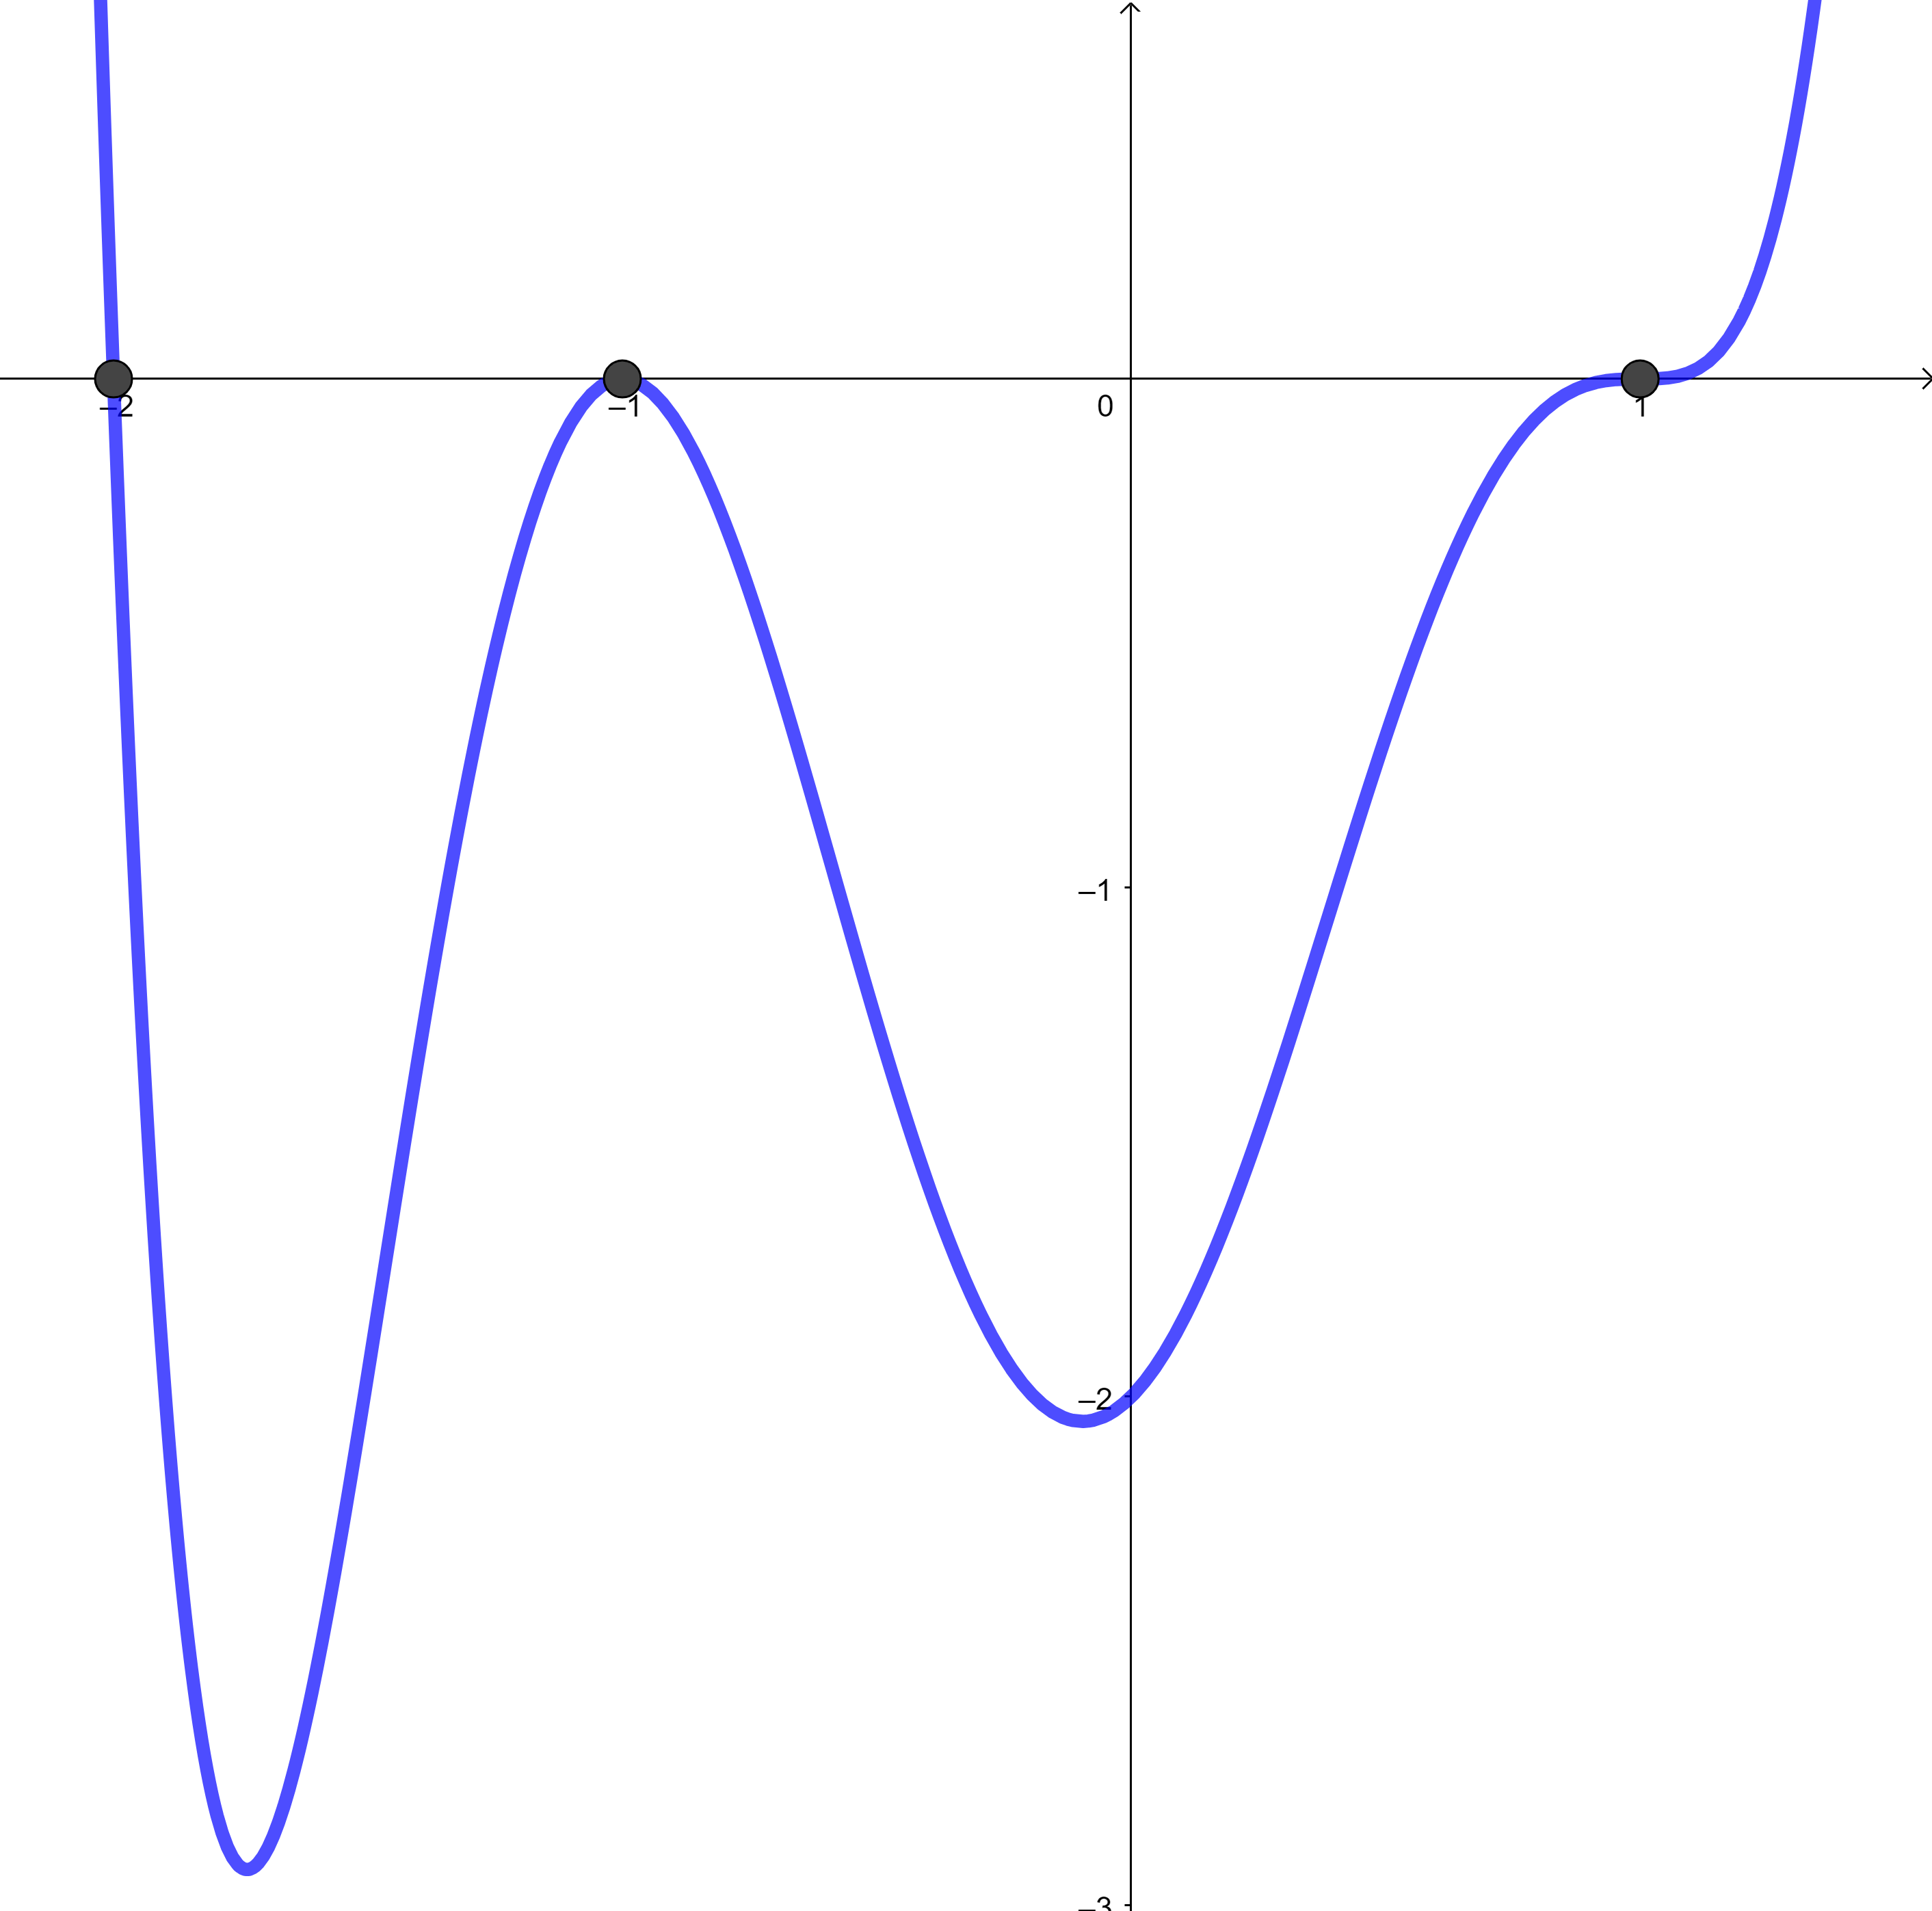
\includegraphics[width=\textwidth]{../Mathematik_1/Bilder/polynome_nullstellen_vielfachheiten.png}
\end{minipage}
	  \begin{minipage}{0.55\textwidth}
		  F�r \( p: x\mapsto (x+2)\cdot (x+1)^2\cdot (x-1)^3 \) gilt:
			  \begin{itemize}
				  \item \(p\) ist in faktorisierter Form gegeben.
				  \item \(p\) besitzt drei unterschiedliche Nullstellen: \(N_p = \{-2,-1,1\}\).
				  \item \(x=-2\) ist eine \textbf{einfache Nullstelle} \(\Rightarrow\) Achse wird geschnitten.
				  \item \(x=-1\) ist eine \textbf{doppelte Nullstelle} \(\Rightarrow\) Achse wird ber�hrt.
				  \item \(x=1\) ist eine \textbf{dreifache Nullstelle} \(\Rightarrow\) Achse wird geschnitten.
				  \item \(p\) verh�lt sich asymptotisch wie die Funktion \(x\mapsto x^6\).
			  \end{itemize}
\end{minipage}
\end{exabox}

\subsection{Parabeln}

In diesem Abschnitt geht es um Polynome zweiten Grades. Polynome zweiten Grades nennt man \textbf{quadratische Funktionen} (\emph{quadratic functions}). Ihre Funktionsgraphen sind \textbf{Parabeln}.

	\begin{itemize}
		\item Es seien $a,b,c\in \mathbb R$ mit $a\not=0$. Eine Funktion der Form \[p:\mathbb R\to \mathbb R, \; x\mapsto a\cdot x^2+b\cdot x+c \] hei�t quadratische Funktion oder Parabel in \textbf{Koeffizientenform}.

		\item Eine Parabel muss keine reellen Nullstellen haben, beispielsweise \(p(x) = x^2+1\). Aber f�r den Fall, dass es reelle Nullstellen gibt, kann man die Parabel faktorisieren.  Eine Parabel mit den Nullstellen $x_1, x_2\in \mathbb R$ (\(x_1 = x_2\) auch erlaubt) besitzt die \textbf{Linearfaktorzerlegung}
			\[p:\mathbb R\to \mathbb R, \; x\mapsto a\cdot (x-x_1) \cdot (x-x_2)\,. \]
	Ausgehend von der Koeffizientenform gilt \[ x_{1,2} = \frac{-b \pm \sqrt{b^2 - 4\cdot a\cdot c}}{2\cdot a}\,.\]

\item Die \textbf{Scheitelpunktform} macht eine andere geometrische Eigenschaft der Parabel unmittelbar sichtbar. F�r
\[
p(x)=a\cdot (x-x_S)^2+y_S
\]
ist
\[
S=(x_S,y_S)
\]
der \textbf{Scheitelpunkt} (\emph{vertex}) der Parabel. Gleichzeitig ist die vertikale Gerade
\[
x=x_S
\]
ihre Symmetrieachse.

F�r \(a>0\) ist der Scheitelpunkt das globale Minimum der Funktion, f�r \(a<0\) das globale Maximum.
\end{itemize}

\begin{exabox}{Verschiedene Darstellungen derselben Parabel}{ }

Die quadratische Funktion
\[
p:\mathbb R\to\mathbb R,
\qquad
x\mapsto x^2-4x-5
\]
ist zun�chst in Koeffizientenform gegeben:
\[
p(x)=x^2-4\cdot x-5.
\]
Aus dieser Darstellung lassen sich unmittelbar die Koeffizienten
\[
a=1,\qquad b=-4,\qquad c=-5
\]
ablesen. Insbesondere zeigt \(a>0\), dass die Parabel nach oben ge�ffnet ist.

Die Nullstellen der Parabel sind
\[
x_1=-1
\qquad\text{und}\qquad
x_2=5.
\]
Damit l�sst sich dieselbe Funktion in Linearfaktoren zerlegen:
\[
p(x)=(x+1)\cdot (x-5).
\]
In dieser Darstellung sind die beiden Nullstellen unmittelbar erkennbar, denn
\[
p(-1)=0
\qquad\text{und}\qquad
p(5)=0.
\]
Der Graph der Parabel schneidet die \(x\)-Achse daher in den Punkten
\[
(-1,0)
\qquad\text{und}\qquad
(5,0).
\]

Durch quadratische Erg�nzung erh�lt man eine dritte Darstellung:
\[
\begin{aligned}
p(x)
&=x^2-4x-5\\
&=x^2-4x+4-4-5\\
&=(x-2)^2-9.
\end{aligned}
\]
Damit liegt die Scheitelpunktform
\[
p(x)=(x-2)^2-9
\]
vor. Aus ihr k�nnen der Scheitelpunkt
\[
S=(2,-9)
\]
und die Symmetrieachse
\[
x=2
\]
unmittelbar abgelesen werden.

Die drei Ausdr�cke
\[
x^2-4\cdot x-5
=
(x+1)\cdot (x-5)
=
(x-2)^2-9
\]
beschreiben also dieselbe quadratische Funktion. Je nach Fragestellung ist jedoch eine andere Darstellung besonders hilfreich:

\[ \begin{array}{lll} \text{Koeffizientenform} &\longrightarrow& \text{Koeffizienten und �ffnung},\\[1mm] \text{Linearfaktorzerlegung} &\longrightarrow& \text{Nullstellen},\\[1mm] \text{Scheitelpunktform} &\longrightarrow& \text{Scheitelpunkt und Symmetrieachse}. \end{array} \]
\end{exabox}
 \newpage % Polynome
\setcounter{exercise}{0} \ifintegriereaufgaben
\section*{Polynome Aufgaben}\label{MA1-polynome-aufgaben}

	Regeln und Beispiele, die zur Bearbeitung der Aufgaben hilfreich sind, finden Sie im Skript\wennreferenzvorhanden{MA1-polynome}{ (Abschnitt \abschnittsverweis{MA1-polynome})} und, falls Sie nicht weiterkommen, schauen Sie \hyperref[MA1-polynome-loesungen]{hier}.
\else
\section{Polynome Aufgaben}\label{MA1-polynome-aufgaben}

	Regeln und Beispiele, die zur Bearbeitung der Aufgaben hilfreich sind, finden Sie im Skript und, falls Sie nicht weiterkommen, schauen Sie \hyperref[MA1-polynome-loesungen]{hier}.
\fi 

\begin{exercisebox}[Symmetrie] %LS
	Zeigen Sie: Wenn der Funktionsterm einer ganzrationalen Funktion einen konstanten Summanden enth�lt, dann ist die Funktion nicht ungerade. 
\end{exercisebox}

\begin{exercisebox}[Umkehrfunktion]
      Die Funktion $f$ mit $f(x)=ax^3+bx,\; a,b\in \mathbb R,$ sei umkehrbar. Welche Bedingung erf�llen die Koeffizienten $a$ und $b$?
\end{exercisebox}

\begin{exercisebox}[Polynom?] %LS p.23 Aufg. 3
	Entscheiden Sie, welche der folgenden Funktionen Polynome sind:
	\begin{eqnarray*} \begin{array}{lll}
			(a)\; x\mapsto 1+\sqrt{2}x & \quad (b)\; x\mapsto 1+2\sqrt{x} &\quad (c)\; x\mapsto (x-1)^2(x-7) \\[1ex]
			(d)\; x\mapsto x^2-\frac3x & \quad (e)\; x\mapsto x^2-\frac{x}{3} &\quad (f)\; x\mapsto  x^2+\sin(x)
		\end{array}
	\end{eqnarray*}
\end{exercisebox}

\begin{exercisebox}[Darstellungen von Parabeln] %Andreas
	Bestimmen Sie von folgenden Parabeln die Linearfaktordarstellung und die Scheitelpunktform.
  \begin{eqnarray*} \begin{array}{ll} 
		  (a)\; x\mapsto -2x^2 -4x+3 \quad \quad   \quad  \quad & (b)\; x\mapsto 5x^2+20x+20 \\[1ex]
		  (c)\; x\mapsto 2x^2+10x  \quad \quad \quad   \quad &(d)\; x\mapsto 4x^2+8x-60
	  \end{array}
  \end{eqnarray*}
\end{exercisebox}

\begin{exercisebox}[Abbildungsvorschrift] %Andreas
	\begin{itemize}
		\item[(a)] Wie m�ssen die Koeffizienten $a,b,c$ lauten, wenn die Parabel $y(x) = ax^2+bx+c$ an den Stellen $x_1 = 1$ und $x_2=-5$ verschwindet und der Funktionswert am Scheitelpunkt $y_S = 18$ betr�gt?
		\item[(b)] Bestimmen Sie ein Polynom $p$ vierten Grades mit den folgenden Eigenschaften: 
			\begin{itemize}
				\item $p$ ist eine gerade Funktion.
				\item $p$ besitzt die Nullstellen $x_1=3$ und $x_2=6$.
				\item $p(0)=-3$
			\end{itemize}
	\end{itemize}
\end{exercisebox}

\begin{exercisebox}[Polynomdivision]
	Zeigen Sie, dass $x_0 = -5$ eine Nullstelle von $p(x) = 3x^3 + 18 x^2 + 9x -30$ ist. Berechnen Sie mit Hilfe der Polynomdivision das Polynom \(q\), f�r das gilt $p(x) = (x-x_0)\cdot q(x)$.
\end{exercisebox}

\begin{exercisebox}[Polynomdivision]
	Bestimmen Sie alle Nullstellen der folgenden Polynome mit Hilfe einer Polynomdivision und stellen Sie die Polynome in Linearfaktorzerlegung dar. Die Polynome besitzen mindestens eine ganzzahlige Nullstelle. 
  \begin{eqnarray*} \begin{array}{ll} 
		  (a)\; x\mapsto x^3-2x^2-5x+6 \quad & (b)\; t\mapsto -2t^4-2t^3-4t+8 \\[1ex]
		  (c)\; x\mapsto x^4-x^3-x^2-x-2 \quad &(d)\; t\mapsto 2t^4+8t^3-12t^2-8t+10
	  \end{array}
  \end{eqnarray*}
\end{exercisebox}

%\begin{exercisebox}[BMI]
%	F�r das Idealgewicht sind zwei g�ngige Formeln in Gebrauch: \begin{center} Idealgewicht in $\mathrm{kg}$ $=$ K�rpergr��e in $\mathrm{cm}$ minus $100$ \end{center}
%	und der Body-Mass-Index, \begin{center} BMI $=$ $\displaystyle{\frac{\textnormal{Gewicht in }\mathrm{kg}}{\left( \textnormal{Koerpergroesse in }\mathrm{m} \right)^2}}\,,$ \end{center} 
%	sollte zwischen $20$ und $25$ liegen.
%	\begin{itemize}
%		\item[(a)] Zeichnen Sie ein Diagramm des Gewichts in Abh�ngigkeit der K�rpergr��e f�r die erste Formel und f�r BMI-Werte von jeweils $20$ und $25$. 
%		\item[(b)] F�r welche K�erpergr��e besitzt das Idealgewicht nach der ersten Formel einen BMI zwischen $20$ und $25$?
%	\end{itemize}
%\end{exercisebox}

%\begin{exercisebox}[Windkraftanlagen]
%	Nehmen Sie an ein Luftmolek�l trifft mit der kinetischen Energie \[ E_{L} = \frac12 m_L v^2\] auf die Rotorfl�chen eines Windkraftwerks. 
%	�berlegen Sie sich Formel, um hieraus n�herungsweise die Leistung $[\frac{\mathrm{N}}{{\mathrm{s}}}]$ eines Windkraftwerks in Abh�ngigkeit der Windgeschwindigkeit $v$ anzugeben.  
%\end{exercisebox}
 \newpage 
\setcounter{satz}{0} \setcounter{def}{0} \setcounter{exa}{0}  \section{Algebraische Gleichungen (+)}\label{MA1-algebraische-gleichungen}

\begin{table}[H]
  \centering
  \begin{tabularx}{\textwidth}{p{0.9\textwidth} p{0.1\textwidth}}
    \toprule
	  \multicolumn{2}{c}{\textbf{�bersicht �ber Lernziele und Voraussetzungen}}\\
    \midrule
	  \textbf{Lernziele} &\\[.5\normalbaselineskip]
\tabitem algebraische Gleichungen erkennen und ihren Grad bestimmen &\\
\tabitem quadratische Gleichungen mit der allgemeinen L�sungsformel l�sen &\\
\tabitem algebraische Gleichungen geeigneter Struktur auf Gleichungen niedrigeren Grades zur�ckf�hren &\\
\tabitem f�r eine algebraische Gleichung eine geeignete L�sungsstrategie ausw�hlen &\\
    \midrule
	  \textbf{Voraussetzungen} &\\[.5\normalbaselineskip]
	  \tabitem Grundlagen & \abschnittsverweis{MA1-mengen-und-logik}-\abschnittsverweis{MA1-aequivalenzumformungen}\\
	  \tabitem Polynome, Nullstellen und Polynomdivision & \abschnittsverweis{MA1-polynome}\\
    \bottomrule
  \end{tabularx}
\end{table}

\ifintegriereaufgaben \noindent �bungsaufgaben zum Thema finden Sie hier: \hyperref[MA1-algebraische-gleichungen-aufgaben]{Aufgaben}
\vspace{0.3cm}
\hrule
\fi

\subsection{Was ist eine algebraische Gleichung?}

Eine Gleichung hei�t \textbf{algebraische Gleichung} (\emph{algebraic equation}),
wenn sie sich durch algebraische Umformungen auf eine Gleichung der Form
\[
p(x)=0
\]
mit einem Polynom \(p\) zur�ckf�hren l�sst.

Im Folgenden stehen insbesondere solche Gleichungen im Mittelpunkt, die nach Ber�cksichtigung ihres Definitionsbereichs durch �quivalenzumformungen auf eine Polynomgleichung zur�ckgef�hrt werden k�nnen.


Eine algebraische Gleichung in Polynomform wird �blicherweise so dargestellt, dass alle Terme auf einer Seite stehen und nach fallenden Potenzen von \(x\) geordnet sind: 
\[
a_n\cdot x^n+a_{n-1}\cdot x^{n-1}+\dots+a_1\cdot x+a_0=0,
\qquad a_n\neq0.
\]
Der h�chste auftretende Exponent \(n\) hei�t der \textbf{Grad} der Gleichung.  Durch Division durch den f�hrenden \underline{Koeffizienten} \randverweis{MA1-polynome} \(a_n\) erh�lt man die
\textbf{normierte Form}
\[
x^n+\frac{a_{n-1}}{a_n}\cdot x^{n-1} +\dots+\frac{a_0}{a_n}=0.
\]

Das folgende Beispiel zeigt den �bergang von einer Bruchgleichung zu einer algebraischen Gleichung in normierter Form.

\begin{exabox}{Algebraische Gleichung}{ }

Gegeben sei die Gleichung
\[
\frac{x^2+7}{x-\pi}
=
\frac{\sqrt{5}}{x^2-9}+3.
\]
Aufgrund der Nenner gilt f�r den Definitionsbereich
\[
D=\mathbb R\setminus\{-3,\pi,3\}.
\]

F�r \(x\in D\) k�nnen die Nenner durch �quivalenzumformungen beseitigt werden:
\[
\begin{array}{c rcl}
& \dfrac{x^2+7}{x-\pi} &=& \dfrac{\sqrt5}{x^2-9}+3 \\[2ex]
\Leftrightarrow& (x^2+7)(x^2-9) &=& \bigl(\sqrt5+3(x^2-9)\bigr)(x-\pi) \\[1ex]
\Leftrightarrow& x^4-2x^2-63 &=& 3x^3-3\pi x^2+(\sqrt5-27)x-\pi\sqrt5+27\pi \\[1ex]
\Leftrightarrow& x^4-3x^3+(3\pi-2)x^2+(27-\sqrt5)x -63-27\pi+\pi\sqrt5 &=&0. 
\end{array}
\]

Damit liegt eine algebraische Gleichung vierten Grades in normierter Form vor.

\medskip
\noindent\textbf{Bemerkungen:}
\begin{itemize}
    \item Die Einschr�nkung
    \[
    x\notin\{-3,\pi,3\}
    \]
    bleibt w�hrend der gesamten Umformung erhalten.
    
    \item Das Multiplizieren mit den Nennern ist nur f�r diejenigen \(x\)
    eine �quivalenzumformung, f�r die diese Nenner von null verschieden sind.
    
    \item Der f�hrende Koeffizient der erhaltenen Polynomgleichung ist bereits
    \(1\). Eine zus�tzliche Division zur Herstellung der normierten Form ist
    daher nicht erforderlich.
\end{itemize}

\end{exabox}

Eine algebraische Gleichung \(n\)-ten Grades zu l�sen bedeutet damit, die Nullstellen des zugeh�rigen \underline{Polynoms}\randverweis{MA1-polynome}  \(n\)-ten Grades zu bestimmen und anschlie�end zu pr�fen, welche dieser Nullstellen im urspr�nglichen Definitionsbereich der Gleichung liegen.
Ein Polynom \(n\)-ten Grades besitzt h�chstens \(n\) verschiedene reelle Nullstellen. Ist sein Grad ungerade, so besitzt es mindestens eine reelle Nullstelle.

%\subsection{Der Satz von Vieta}
%
%Bleiben wir bei der algebraischen Gleichung des Beispiels:
%  $$  x^4  + \displaystyle{\frac37}\cdot x^3 + \displaystyle{\frac{2+3\pi}{7}}\cdot x^2 - \sqrt{5}\cdot x + 9 = 0\,.$$
%
%  Angenommen (angenommen!), das Polynom \[ p: x\mapsto x^4  + \displaystyle{\frac37} \cdot x^3 + \displaystyle{\frac{2+3\pi}{7}}\cdot x^2 - \sqrt{5} \cdot x + 9 \] l�sst sich komplett in Linearfaktoren zerlegen, dann gibt es vier reelle Nullstellen \(x_1, x_2, x_3\) und \(x_4\) mit 
%  $$p(x) = (x-x_1) \cdot (x-x_2) \cdot (x-x_3) \cdot (x-x_4) \stackrel{!}{=} x^4  + \displaystyle{\frac37} \cdot x^3 + \displaystyle{\frac{2+3\pi}{7}} \cdot x^2 - \sqrt{5} \cdot x + 9 \,. \quad (*)$$
%  Wir haben in \((*)\) o.B.d.A.\footnote{o.B.d.A. bedeutet "\,ohne Beschr�nkung der Allgemeinheit"} die Linearfaktorzerlegung zur Darstellung von \(p\) angesetzt.\footnote{Erinnern Sie sich: dieser Ansatz ist immer dann optimal wenn es um die Nullstellen von \(p\) geht!} 
%
%  Die algebraische Gleichung haben wir gel�st, wenn wir konkrete Zahlenwerte f�r die \(x_1,\cdots,x_4\) bestimmen k�nnen und dies gelingt durch Ausmultiplizieren und \textbf{Koeffizientenvergleich}:\marginpar{Aufgaben}
%
%\begin{exabox}{Bestimmung von Nullstellen: Ansatz ausmultiplizieren und Koeffizientenvergleich}{}
%\begin{eqnarray*}  
%\lefteqn{x^4  + \displaystyle{\frac37} x^3 + \displaystyle{\frac{2+3\pi}{7}} x^2 - \sqrt{5} x + 9 \stackrel{!}{=} (x-x_1)\cdot (x-x_2)\cdot (x-x_3)\cdot (x-x_4)}\\
%  &=& x^4 - x^3\left(x_1 + x_2 +x_3+ x_4\right) + x^2\left( x_1x_2+x_1x_3+x_1x_4+x_2x_3+x_2x_4+x_3x_4 \right)\\&& - x\left( x_1x_3x_4+x_2x_3x_4+x_1x_2x_3+x_1x_2x_4 \right) + \left( x_1x_2x_3x_4\right)\\ 
%  &&\\
%  &\Rightarrow& \begin{cases}  
%	  -x_1 - x_2 - x_3 - x_4 &= \displaystyle{\frac37} \\   
%	  x_1x_2+x_1x_3+x_1x_4+x_2x_3+x_2x_4+x_3x_4  &= \displaystyle{\frac{2+3\pi}{7}} \\
%	  -x_1x_3x_4-x_2x_3x_4-x_1x_2x_3-x_1x_2x_4 &= -\sqrt{5} \\
%  x_1\cdot x_2\cdot x_3\cdot x_4 &= 9 \end{cases} 
%\end{eqnarray*}
%\end{exabox}
%
%\noindent\textbf{Bemerkungen:}
%\begin{itemize}
%	\item Unter den Voraussetzungen, dass nur reelle Nullstellen vorliegen, geht das nat�rlich auch f�r Polynome beliebigen Grades.
%	\item Das geschilderte Vorgehen zur Nullstellenbestimmung durch Koeffizientenvergleich hei�t  "\,Satz von Vieta".
%	\item Der Satz von Vieta f�hrt zu einem System nicht-linearer Gleichungen, das im Allgemeinen schwer analytisch zu l�sen ist. Eine Ausnahme sind quadratische Gleichungen.\marginpar{\small Aufgabe}
%\end{itemize}

\subsection{Quadratische Gleichungen}

Eine quadratische Gleichung kann durch quadratische Erg�nzung auf eine bereits
bekannte Gleichung mit einer zweiten Potenz zur�ckgef�hrt werden. Aus
\[
a\cdot x^2+b\cdot x+c=0,
\qquad a\neq0,
\]
folgt zun�chst durch Division durch \(a\)
\[
x^2+\dfrac ba x+\dfrac ca=0.
\]
Der Ausdruck aus \(x^2\) und \(x\) wird nun zu einem vollst�ndigen Quadrat
erg�nzt:\marginpar{Aufgaben}
  $$
  \underbrace{ x^2 + \frac{b}{a}x + \frac{b^2}{4a^2}}_{\displaystyle{ = \left(x + \frac{b}{2a}\right)^2}} + \frac{c}{a}  - \frac{b^2}{4a^2} = 0\,.
  $$
Also ist die urspr�ngliche Gleichung �quivalent zu:
$$\left(x + \frac{b}{2a}\right)^2  = \frac{\textcolor{blue}{b^2- 4\,c\cdot a}}{a^2} \,. $$
  Der Ausdruck
\[
	\Delta:= \textcolor{blue}{b^2-4\,a\cdot c}
\]
hei�t \textbf{Diskriminante} (\emph{discriminant}). Das Vorzeichen der Diskrinimante Vorzeichen bestimmt, wie viele reelle L�sungen die quadratische Gleichung besitzt.
\begin{theorembox}{L�sungsformel f�r quadratische Gleichungen}{ }
  \begin{eqnarray*}
    \begin{cases} 
      \Delta > 0 \Rightarrow x_{1,2} = \displaystyle{\frac{-b \pm \sqrt{ b^2 - 4ac}}{2a}} \quad (*)\,,\\
      \Delta = 0 \Rightarrow x_{1,2} = \displaystyle{\frac{-b}{2a}}\,,\\
      \Delta < 0 \Rightarrow \textnormal{keine reellen L\"osungen}\,.
    \end{cases}
    \end{eqnarray*}
 \end{theorembox}

 Die drei F�lle besitzen eine geometrische Interpretation.\marginpar{ \small \href{https://www.geogebra.org/m/PHfR2APJ}{GeoGebra}}
Die L�sungen der quadratischen Gleichung
\[
ax^2+bx+c=0
\]
sind genau die Nullstellen der zugeh�rigen Parabel
\[
p(x)=ax^2+bx+c.
\]
Daher schneidet die Parabel f�r \(\Delta>0\) die \(x\)-Achse in zwei Punkten, ber�hrt sie f�r \(\Delta=0\) in ihrem Scheitelpunkt und besitzt f�r \(\Delta<0\) keinen Schnittpunkt mit der \(x\)-Achse.

\subsection{Gleichungen h�herer Ordnung}

Liebt eine Gleichung h�heren Grades vor, dann ist f�r die Wahl einer L�sungsstrategie zun�chst die Struktur der Gleichung
entscheidend:

\begin{itemize}
    \item Eine quadratische Gleichung kann durch quadratische Erg�nzung oder mit der allgemeinen L�sungsformel gel�st werden.
    
    \item Ist bei einer Gleichung h�heren Grades bereits eine Nullstelle bekannt, kann der zugeh�rige Linearfaktor abgespalten und der Grad durch Polynomdivision reduziert werden.
    
    \item Tritt die Unbekannte nur in bestimmten Potenzen auf, kann eine geeignete Substitution die Gleichung auf einen niedrigeren Grad zur�ckf�hren.
\end{itemize}

\subsubsection*{Reduktion des Grades durch Polynomdivision}

\begin{exabox}{Gradreduktion durch Polynomdivision}{ }

Gegeben sei die algebraische Gleichung
\[
x^3-2\cdot x^2-5\cdot x+6=0.
\]
F�r das zugeh�rige Polynom
\[
p(x)=x^3-2x^2-5x+6
\]
sei die Nullstelle \(x_1=1\) bereits bekannt. 
Damit ist \((x-1)\) ein Linearfaktor von \(p\), und die Polynomdivision durch
\((x-1)\) geht ohne Rest auf:
\[
\begin{array}{rcrcrcl}
(x^3&-&2x^2&-&5x&+&6):(x-1)=x^2-x-6\\[1ex]
-(x^3&-&x^2)&&&&\\ \hline
&&-x^2&-&5x&+&6\\[1ex]
&&-(-x^2&+&x)&&\\ \hline
&&&&-6x&+&6\\[1ex]
&&&&-(-6x&+&6)\\ \hline
&&&&&&0
\end{array}
\]
Damit l�sst sich das Polynom schreiben als
\[
p(x)=(x-1)\cdot (x^2-x-6).
\]
Die urspr�ngliche Gleichung ist daher �quivalent zu
\[
(x-1)(x^2-x-6)=0.
\]
Der verbleibende quadratische Faktor kann weiter zerlegt werden:
\[
x^2-x-6=(x-3)\cdot (x+2).
\]
Somit gilt
\[
	p(x) = (x-1)(x-3)(x+2)
\]
Ein Produkt ist genau dann null, wenn mindestens einer seiner Faktoren null
ist. Daher ergeben sich die drei L�sungen
\[
	p(x) = 0 \Leftrightarrow x\in \mathbb L=\{-2,1,3\}.
\]

Durch das Abspalten des bekannten Linearfaktors wurde die Gleichung dritten
Grades auf eine quadratische Gleichung zur�ckgef�hrt. Allgemein kann eine
bekannte Nullstelle einer Polynomgleichung h�heren Grades auf diese Weise
genutzt werden, um den Grad der noch zu l�senden Gleichung zu reduzieren.

\end{exabox}

\subsubsection*{Reduktion des Grades durch Substitution}

\begin{exabox}{Gradreduktion durch Substitution}{ }

Gegeben sei die algebraische Gleichung
\[
x^4-5\cdot x^2+4=0.
\]
Obwohl es sich um eine Gleichung vierten Grades handelt, besitzt sie eine
besondere Struktur: Die Unbekannte \(x\) tritt nur in den Potenzen
\(x^4\) und \(x^2\) auf. Da
\[
x^4=(x^2)^2
\]
gilt, kann die Substitution \( z = x^2\) verwendet werden. Damit wird aus der Gleichung vierten Grades in \(x\) die
quadratische Gleichung in \(z\)
\[
z^2-5\cdot z+4=0.
\]
Der quadratische Term l�sst sich faktorisieren:
\[
(z-1)(z-4)=0 \Leftrightarrow 
z_1=1
\qquad\text{und}\qquad
z_2=4.
\]

Damit ist zun�chst die Gleichung in der neuen Variablen \(z\) gel�st. F�r
die L�sungen der urspr�nglichen Gleichung muss nun die Substitution \(z=x^2\)
r�ckg�ngig gemacht werden.

\[
	\left\{\begin{array}{rcl l} z_1&=&1 \Rightarrow x^2=1 \Longleftrightarrow & x=\pm1 \\
	z_2&=&4 \Rightarrow x^2=4 \Longleftrightarrow & x=\pm2\end{array}\right. 
\]
Damit besitzt die urspr�ngliche Gleichung die vier L�sungen \(\mathbb L=\{-2,-1,1,2\}.\)

Bei einer Substitution muss nach dem L�sen der vereinfachten Gleichung stets
zur urspr�nglichen Variablen zur�ckgekehrt werden. 
\end{exabox}

Nicht jede algebraische Gleichung l�sst sich mit den hier genannten Ideen
Verfahren analytisch l�sen. F�r allgemeine Gleichungen dritten und vierten
Grades existieren zwar ebenfalls geschlossene L�sungsformeln, diese sind
jedoch wesentlich aufwendiger und werden hier nicht behandelt.

F�r allgemeine algebraische Gleichungen f�nften oder h�heren Grades existiert
keine L�sungsformel, die mit der allgemeinen L�sungsformel f�r
quadratische Gleichungen vergleichbar w�re. Einzelne Gleichungen h�heren
Grades k�nnen aufgrund ihrer besonderen Struktur dennoch exakt l�sbar sein.

Ist eine exakte L�sung nicht zug�nglich oder nicht zweckm��ig, k�nnen
Nullstellen numerisch angen�hert werden. Beispiele daf�r sind das
Bisektionsverfahren und das Newton-Verfahren. Solche Verfahren werden sp�ter
im Abschnitt \underline{Numerische N�herung}\randverweis{MA1-lokale-linearitaet}
behandelt.
 \newpage % Algebraische Gleichungen
\setcounter{exercise}{0} \ifintegriereaufgaben
\section*{Algebraische Gleichungen Aufgaben}\label{MA1-algebraische-gleichungen-aufgaben}

	Regeln und Beispiele, die zur Bearbeitung der Aufgaben hilfreich sind, finden Sie im Skript\wennreferenzvorhanden{MA1-algebraische-gleichungen}{ (Abschnitt \abschnittsverweis{MA1-algebraische-gleichungen})} und, falls Sie nicht weiterkommen, schauen Sie \hyperref[MA1-algebraische-gleichungen-loesungen]{hier}.
\else
\section{Algebraische Gleichungen Aufgaben}\label{MA1-algebraische-gleichungen-aufgaben}

	Regeln und Beispiele, die zur Bearbeitung der Aufgaben hilfreich sind, finden Sie im Skript und, falls Sie nicht weiterkommen, schauen Sie \hyperref[MA1-algebraische-gleichungen-loesungen]{hier}.
\fi 

\begin{exercisebox}[Gleichungen] %LS p.29, Aufgabe 7
  \begin{itemize}
	  \item[(a)] Zeigen Sie, dass der Graph der Funktion $f: x \mapsto x^3-2x^2-3x+10$ die $x$-Achse nur im Punkt $S(-2|0)$ schneidet.
	  \item[(b)] Die Gerade $g$ geht durch $S$ und hat die Steigung $2$. Berechnen Sie alle Schnittpunkte von $g$ mit dem Graphen von $f$.
  \end{itemize}
\end{exercisebox}

\begin{exercisebox}[Gleichungen] %LS p. 29, Aufgabe 6 b) und d)
  Bestimmen Sie durch Probieren eine Nullstelle und berechnen Sie danach die weiteren Nullstellen.
  \begin{itemize}
	  \item[(a)] $f(x) = x^3+x^2-4x-4$
	  \item[(b)] $f(x) = 4x^3-20x^2-x + 110$
  \end{itemize}
\end{exercisebox}

\begin{exercisebox}[Gleichungen]
	Geben Sie die L�sungsmengen der folgenden Gleichungen an:
	\begin{eqnarray*}
		\begin{array}{ll} (a) \; x^2-2 x -7 = 0  \quad \quad \quad & (b)\; x^3-6 x^2 - x + 30 = 0 \\[1ex]
			(c) \; 2x^3-5 x^2 -10 x = 0 \quad \quad \quad \quad & (d) \; x^4-13 x^2+36 = 0
		\end{array}
	\end{eqnarray*}
\end{exercisebox}

\begin{exercisebox}[Anwendung: Newton-Verfahren]
	\begin{itemize}
		\item[(a)] Betrachten Sie die Funktion \[ f: x\mapsto \sin(x) - \frac12 x - \frac{1}{10}\,.\] Formulieren Sie das Newton-Verfahren zur Bestimmung einer Nullstelle von $f$ f�r den Startwert $x_0 = \frac{1}{10}$. F�hren Sie drei Iterationen durch. Hinweis: $f': x\mapsto \cos(x) - \frac12$. 
			%Es gilt $f'(x) = \cos(x) - \frac12$ und wir erhalten \[ x_{m+1} = x_m - \frac{f(x_m)}{f'(x_m)} = x_m - \frac{\sin(x_m) - \frac12 x_m - \frac{1}{10} }{\cos(x_m) - \frac12 }\] Die ersten drei Iterierten lauten \[ x_1 \approx 0.202, \quad x_2\approx 0.203, \quad x_3\approx 0.202\,.\]
		\item[(b)] 
	Bestimmen Sie eine Folge, die sich f�r gro�e $n$ an $\sqrt{5}$ ann�hert. Hinweis: Betrachten Sie $f:x\mapsto x^2-5$ mit $f': x\mapsto 2x$.
\item[(c)]
	Berechnen Sie die ersten drei Iterierten des Newton-Verfahrens zur Funktion \[ f:x\mapsto x^3-2y+2\] mit Startwert $x_0=0$. Konvergiert das Newton-Verfahren? Interpretieren Sie das Ergebnis.
	%Die Newton-Iteration lautet \[ x_{m+1} = x_m - \frac{f(x_m)}{f'(x_m)} = x_m - \frac{x_m^2 - 2x_m + 2 }{ 3 x_m^2 -2}\,.\] Es gilt also \[ x_0 = 1, \quad x_1 = 1-\frac11 = 0,\quad x_2 = 0 - \frac{2}{-2} = 1, \quad x_3 = 0\,.\]
	%Es werden abwechselnd die Werte $0$ und $1$ angenommen, so dass eine Konvergenz der Iterierten ausgeschlossen ist. Der Startwert $x_0 =0$ war offenbar nicht nah genug an der L�sung dran. 
		%\item[(d)] Berechne mit Hilfe des Newtonschen N�herungsverfahren die Nullstellen der folgenden Funktion auf zwei Nachkommastellen genau:  \[ f:x\mapsto x^3-5x^2-4x+2 \] Hinweis: $f':x\mapsto 3x^2-10x -4$
	\end{itemize}
\end{exercisebox}

%
%\begin{exercisebox}[Mathematik lesen, Fehlerabsch�tzung]
%  $|\left(x-f(x)f'(x)\right) - \underline x| \leq c\,|x-\underline x|^2\,.$ 
%  \end{exercisebox}
 \newpage 
\setcounter{satz}{0} \setcounter{def}{0} \setcounter{exa}{0}  \section{Rationale Funktionen}\label{MA1-rationale-funktionen}

\begin{table}[H]
  \centering
  \begin{tabularx}{\textwidth}{p{0.9\textwidth} p{0.1\textwidth} }
    \toprule
	  \multicolumn{2}{c}{\textbf{�bersicht �ber Lernziele und Voraussetzungen}}\\
    \midrule
	  \textbf{Lernziele} &\\[.5\normalbaselineskip]
\tabitem rationale und gebrochenrationale Funktionen erkennen &\\
\tabitem Definitionsl�cken, Nullstellen und Polstellen systematisch bestimmen &\\
\tabitem hebbare Definitionsl�cken von Polstellen unterscheiden &\\
\tabitem das Verhalten f�r \(x\to\pm\infty\) und in der N�he von Polstellen untersuchen &\\
\tabitem Asymptoten gebrochenrationaler Funktionen bestimmen &\\
\tabitem gebrochenrationale Funktionen anhand ihrer charakteristischen Eigenschaften qualitativ skizzieren &\\
\tabitem eine gebrochenrationale Funktion aus gegebenen Eigenschaften konstruieren &\\[.5\normalbaselineskip]
    \midrule
	  \textbf{Voraussetzungen}& \\[.5\normalbaselineskip]
\tabitem Polynome, Nullstellen und Linearfaktorzerlegung & \abschnittsverweis{MA1-polynome}\\
\tabitem algebraische Gleichungen & \abschnittsverweis{MA1-algebraische-gleichungen}\\
    \bottomrule
  \end{tabularx}
\end{table}

\ifintegriereaufgaben \noindent �bungsaufgaben zum Thema finden Sie hier: \hyperref[MA1-rationale-funktionen-aufgaben]{Aufgaben}
\vspace{0.3cm}
\hrule
 \fi

\subsection{Was ist eine rationale Funktion?}

Eine Funktion \(f\) hei�t \textbf{rationale Funktion}
(\emph{rational function}), wenn ihre Abbildungsvorschrift in der Form
\[
f(x)=\frac{p(x)}{q(x)}
\]
mit \underline{Polynome}\randverweis{MA1-polynome} \(p\) und \(q\) und \(q\not\equiv0\) dargestellt werden kann.

Der maximale \underline{Definitionsbereich}\randverweis{MA1-funktionen} besteht aus allen reellen Zahlen, f�r die
das Nennerpolynom nicht null ist:
\[
D_f
=
\{x\in\mathbb R:q(x)\neq0\}
=
\mathbb R\setminus\{x\in\mathbb R:q(x)=0\}.
\]
Die Nullstellen des Nennerpolynoms sind die \textbf{Definitionsl�cken} der rationalen Funktion. Um Definitionsl�cken zu finden ist also eine \underline{algebraische} \underline{Gleichung}\randverweis{MA1-algebraische-gleichungen} zu l�sen.

\noindent \textbf{Bemerkungen:}
	\begin{itemize}
\item Polynome sind besonders einfache rationale Funktionen. Bei ihnen ist das Nennerpolynom eine Konstante $(\not=0)$,
\item Ist nach vollst�ndigem K�rzen der Funktion das Nennerpolynom nicht konstant, so hei�t die Funktion \textbf{gebrochenrational}.\marginpar{Aufgabe}
	\end{itemize}

Die Definitionsl�cken einer gebrochenrationalen Funktion k�nnen zu \textbf{Polstellen} f�hren.  

Eine Definitionsl�cke muss nicht notwendigerweise eine Polstelle sein.  Entscheidend ist, ob sie beim K�rzen gemeinsamer Faktoren von Z�hler und Nenner verschwindet.

\noindent{\textbf{Merke:}} Bleibt der entsprechende Linearfaktor nach vollst�ndigem K�rzen im Nenner erhalten, liegt eine \textbf{Polstelle} (\emph{pole}) vor. Verschwindet der Faktor vollst�ndig aus dem Nenner, liegt eine \textbf{hebbare Definitionsl�cke} (\emph{removable singularity}) vor.	

In der N�he einer Polstelle wachsen die Funktionswerte betragsm��ig unbeschr�nkt. Je nach \textbf{Vielfachheit} und Vorzeichen k�nnen dabei unterschiedliche Verl�ufe auftreten.  Ist nach vollst�ndigem K�rzen der Faktor
\[
(x-x_0)^k
\]
im Nenner enthalten, w�hrend der Z�hler bei \(x_0\) von null verschieden ist,
so besitzt \(f\) bei \(x_0\) eine Polstelle der Vielfachheit \(k\). F�r das Verhalten beim �berschreiten der Polstelle gilt:\marginpar{Aufgaben}
\begin{itemize}
    \item Ist \(k\) ungerade, wechselt die Funktion an der Polstelle ihr Vorzeichen.
    \item Ist \(k\) gerade, findet kein Vorzeichenwechsel statt.
\end{itemize}

%\subsection{Anwendung: $z$-Transformation}
%
%Rationale Funktionen treten vor allem auf, wenn man Filter oder Regelungsanlagen beschreibt, die R�ckkopplungen enthalten. Eines der einfachsten Beispiele daf�r sind digitale Filter (genauer gesagt, kausale lineare Filter). Hier arbeitet man mit Signalen, die mit einer festen Frequenz abgetastet werden. Sie k�nnen zueinander addiert, mit Konstanten multipliziert und um eine feste Anzahl von Abtastzyklen verz�gert werden - zum Beispiel so:
%\begin{tcolorbox}
%  Bild
%\end{tcolorbox}
%
%Jedes  Signal,  das  hier  vorkommt,  l�sst  sich  in  eine  rationale  Funktion  einer k�nstlichen Variablen $z$ �bersetzen: 
%\begin{tcolorbox}
%  Bild
%  $ x\mathrm{-Achsenabschnitt} \, z ^{-\mathrm{Nummer des Samples}} $
%  $ \mathrm{diskretes Signal} \to 1 - 1x^{-1} z^{-1} + 2 z^{-2} - 2 z^{-3} + z^{-4} $
%\end{tcolorbox}
%
%Die Funktion auf der rechten Seite nennt sich die $z$-Transformierte des Signals. Die Summe zweier Signale hat die Summe der beiden $z$-Transformierten; ein festes Vielfaches eines Signals hat das Vielfache seiner $z$-Transformierten. Verz�gert man ein Signal um $n$ Abtastzyklen, wird seine $z$-Transformierte mit $z^{-n}$ multipliziert. Ist $x(z)$ die $z$-Transformierte des Eingangssignals des Filters aus dem Beispiel und $y(z)$ die $z$-Transformierte des Ausgangssignals, findet man:
%\begin{tcolorbox}
%  $ x(z) \to  x(z) z^{-n}\,. $
%\end{tcolorbox}
%
%Die Wirkung des Filters wird also durch eine rationale Funktion beschrieben. Digitale Filter zu entwerfen, hei�t vor allem, sich solche rationalen Funktionen passend aus zu denken. Man kann nun sagen, wie das Filter auf einen Impuls Nummer des Samples 
%\begin{tcolorbox}
%\end{tcolorbox}
%
%reagiert (die sogenannte Impulsantwort):
%\begin{tcolorbox}
%\end{tcolorbox}

Es kann vorkommen, dass Nullstellen der Z�hlerfunktion auch gleichzeitig Nullstellen der Nennerfunktion sind, zum Beispiel hier:
\[f:x\mapsto \dfrac{ (x - 2)\cdot (x + 1) }{ ( x - 2) \cdot (x - 3)\cdot (x + 1)}\,.\]
K�nnen wir so eine Funktion k�rzen? Ja, aber nur unter Beibehaltung des Definitionsbereichs:
\begin{exabox}{Hebbare Definitionsl�cke und Polstelle}{ }
	\hspace{-0.3cm}\begin{minipage}{0.4\textwidth}
	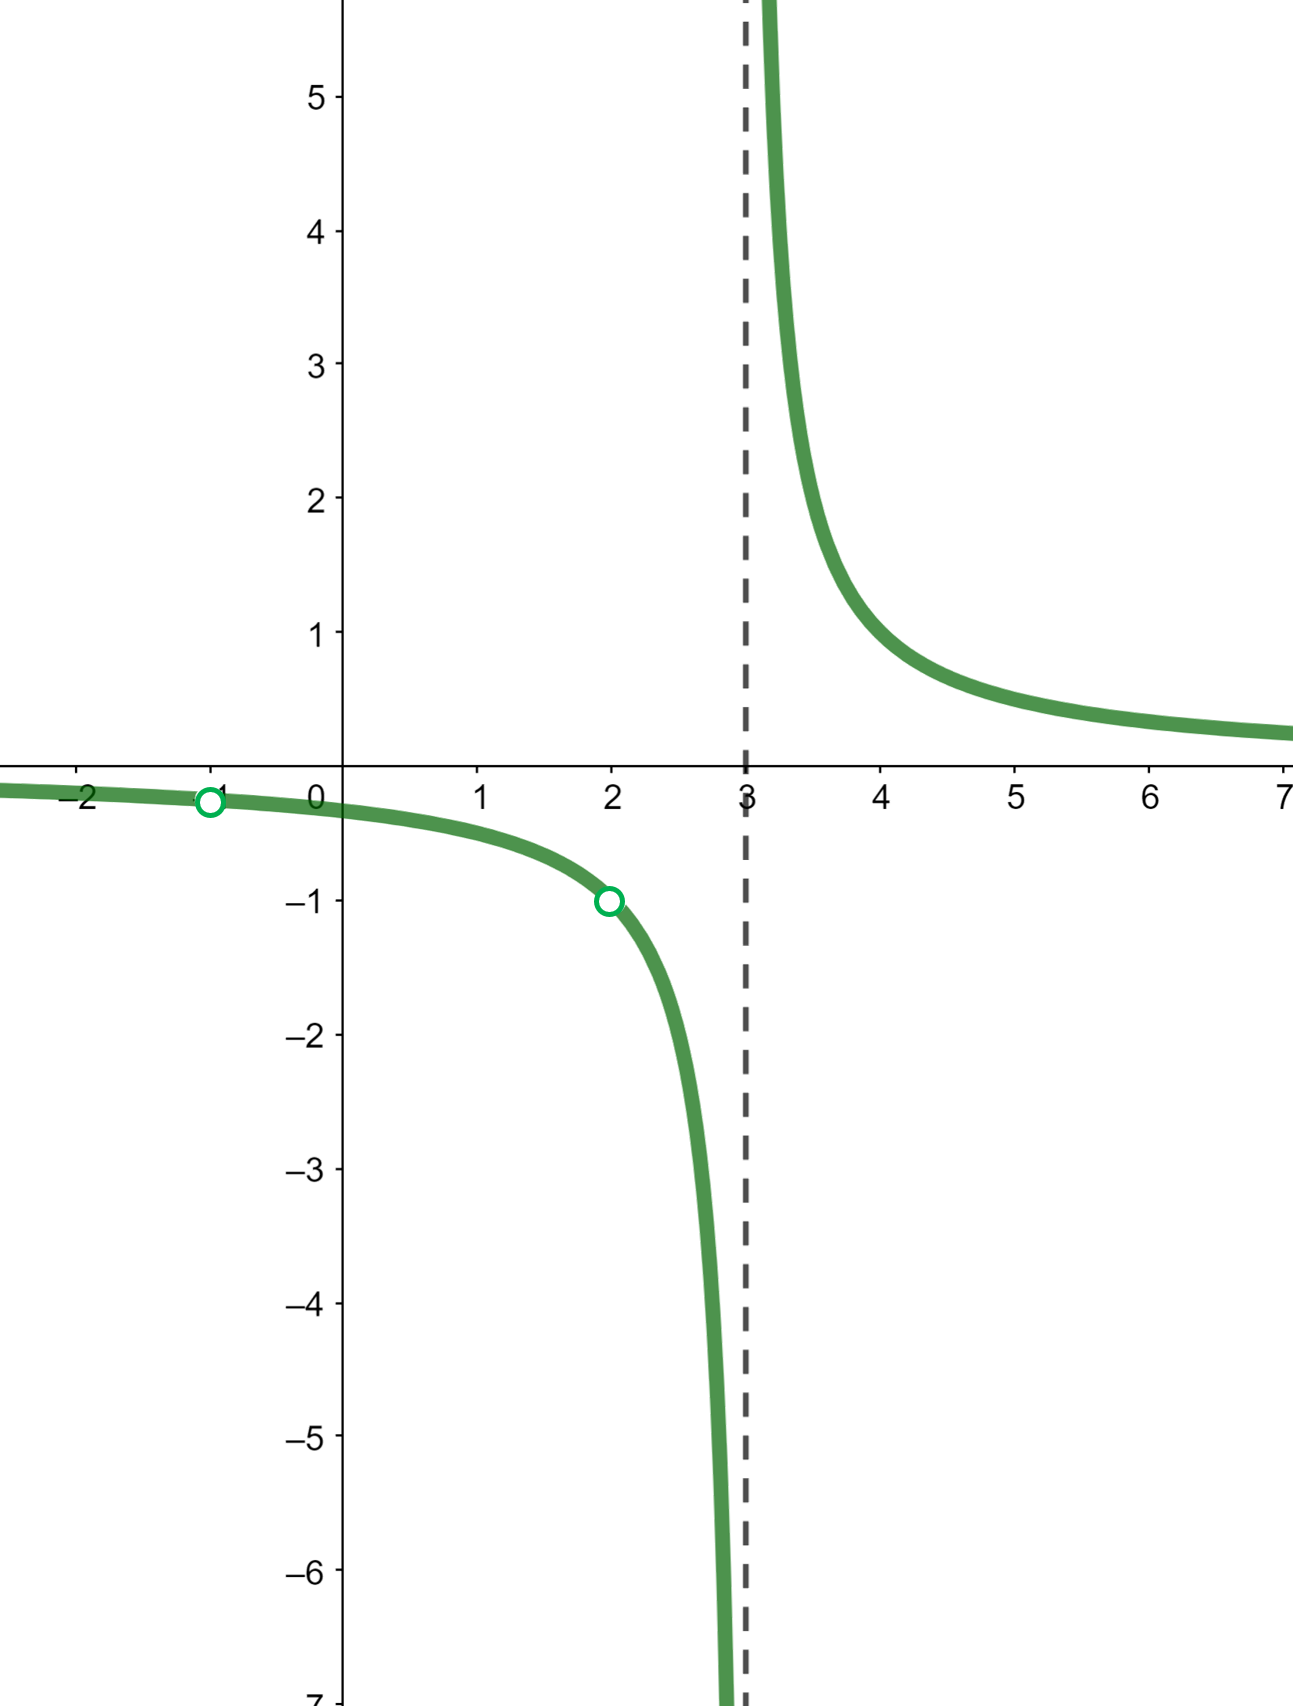
\includegraphics[width=\textwidth]{../Mathematik_1/Bilder/rationale_funktionen_hebbare_luecken_polstelle.png}
\end{minipage}
	\begin{minipage}{0.6\textwidth}
		Das Bild zeigt den Graph der Funktion \[  f: x \mapsto \dfrac{p(x)}{q(x)} = \dfrac{ (x - 2)\cdot (x+1)}{ (x - 2) \cdot (x - 3)\cdot (x + 1)}\,.\] 

		Den Funktionsverlauf von \(f\) analysieren wir wie folgt:
		\begin{itemize}
			\item Nullstellen des Z�hlers: \(N_p = \{-1, 2\}\).
			\item Nullstellen des Nenners: \(N_q = \{-1,2,3\}\).
			\item Definitionsbereich: \(D_f = \mathbb R\setminus \{ -1,2,3\} \)
			\item Nullstellen von $f$: \( N_f = \{ \} \not= N_p\)!
			\item Polstellen von \(f\): \(P_f = \{3\} \not= N_q\)!
			\item Asymptote von \(f\) f�r \(|x|\to\infty\): die \(x\)-Achse
		\end{itemize}
\end{minipage}
\end{exabox}
Die gebrochenrationale Funktion \(f\) besitzt drei Definitionsl�cken, von denen eine eine Polstelle mit Vorzeichenwechsel ist. Der Bruch ist nicht vollst�ndig gek�rzt -- die Funktionsabbildung kann noch vereinfacht werden:
		\[
			f: \mathbb R\setminus \{ -1, 2, 3\} \to \mathbb R\,, \dfrac{ (x-2)\cdot (x+1) }{(x-2)\cdot (x-3)\cdot (x+1)} = \dfrac{1}{x-3}\,. 
\]

Das Beispiel zeigt: eine Nullstelle des Z�hlerpolynoms ist nur dann eine Nullstelle der rationalen Funktion, wenn sie zum Definitionsbereich der Funktion geh�rt. Ist sie gleichzeitig eine Nullstelle des Nennerpolynoms, liegt dort zun�chst eine Definitionsl�cke vor.

Die Definitionsl�cken, die man in der gek�rzten Variante nicht mehr erkennen kann, erzeugen keine Polstellen, sondern "\,L�cher"\, im Graphen. In einer Zeichnung markiert man diese L�cher normalerweise mit einem kleinen, unausgef�llten Kringel auf dem Funktionsgraphen. 

Ist die Definitionsl�cke bei $x_0$ mehrmals vorhanden, d.h. auch nach vollst�ndigem K�rzen der Funktion ist ein \underline{Linearfaktor}\randverweis{MA1-polynome} $(x-x_0)$ im Nenner enthalten, so findet man bei $x_0$ nach wie vor eine Polstelle und kein "\,Loch"\, im Graphen. Ein Beispiel:\marginpar{Aufgaben}
\begin{exabox}{K�rzen bei einer Polstelle}{ }
	\hspace{-0.3cm}\begin{minipage}{0.4\textwidth}
	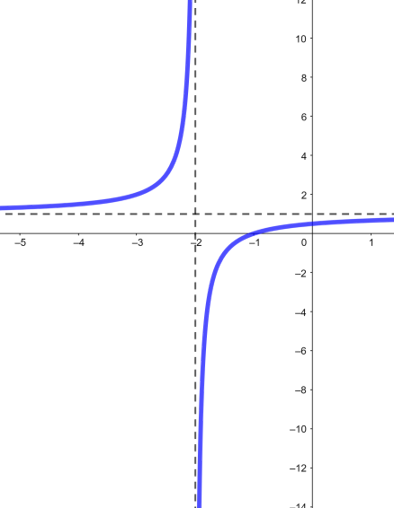
\includegraphics[width=\textwidth]{../Mathematik_1/Bilder/rationale_funktionen_polstelle_nach_kuerzen.png}
\end{minipage}
	\begin{minipage}{0.6\textwidth}
		Das Bild zeigt den Graph der Funktion \[  f: x \mapsto \dfrac{p(x)}{q(x)} = \dfrac{(x+1)\cdot (x+2)}{(x+2)^2}\,.\] 

		Den Funktionsverlauf von \(f\) analysieren wir wie folgt:
		\begin{itemize}
			\item Nullstellen des Z�hlers: \(N_p = \{-1,-2\}\).
			\item Nullstellen des Nenners: \(N_q = \{-2\}\).
			\item Definitionsbereich von \(f\): \(D =\mathbb R\setminus \{ -2\} \)
			\item Nullstellen von $f$: \( N_f = \{-1\} \not= N_p\)!
			\item Polstellen von \(f\): \(P_f = \{-2\} \not= N_q \)!
			\item Asymptote von \(f\) f�r \(|x|\to\infty\): \(x\mapsto 1\)
		\end{itemize}
	\end{minipage}	
\end{exabox}

Die gebrochenrationale Funktion \(f\) besitzt bei \(x=-2\) eine Definitionsl�cke. Obwohl ein gemeinsamer Linearfaktor gek�rzt werden kann, bleibt der Faktor \((x+2)\) einmal im Nenner erhalten. Die Definitionsl�cke ist daher eine Polstelle mit Vorzeichenwechsel.  Der Bruch ist nicht vollst�ndig gek�rzt -- die Funktionsabbildung kann noch vereinfacht werden:
		\[
			f: \mathbb R\setminus \{ -2\} \to \mathbb R\,, x\to \dfrac{ (x+1)\cdot (x+2) }{(x+2)^2} = \dfrac{x+1}{x+2}\,. 
\]

Und noch ein Beispiel
\begin{exabox}{Hebbare Definitionsl�cke ohne Polstelle}{ }
	\hspace{-0.3cm}\begin{minipage}{0.4\textwidth}
	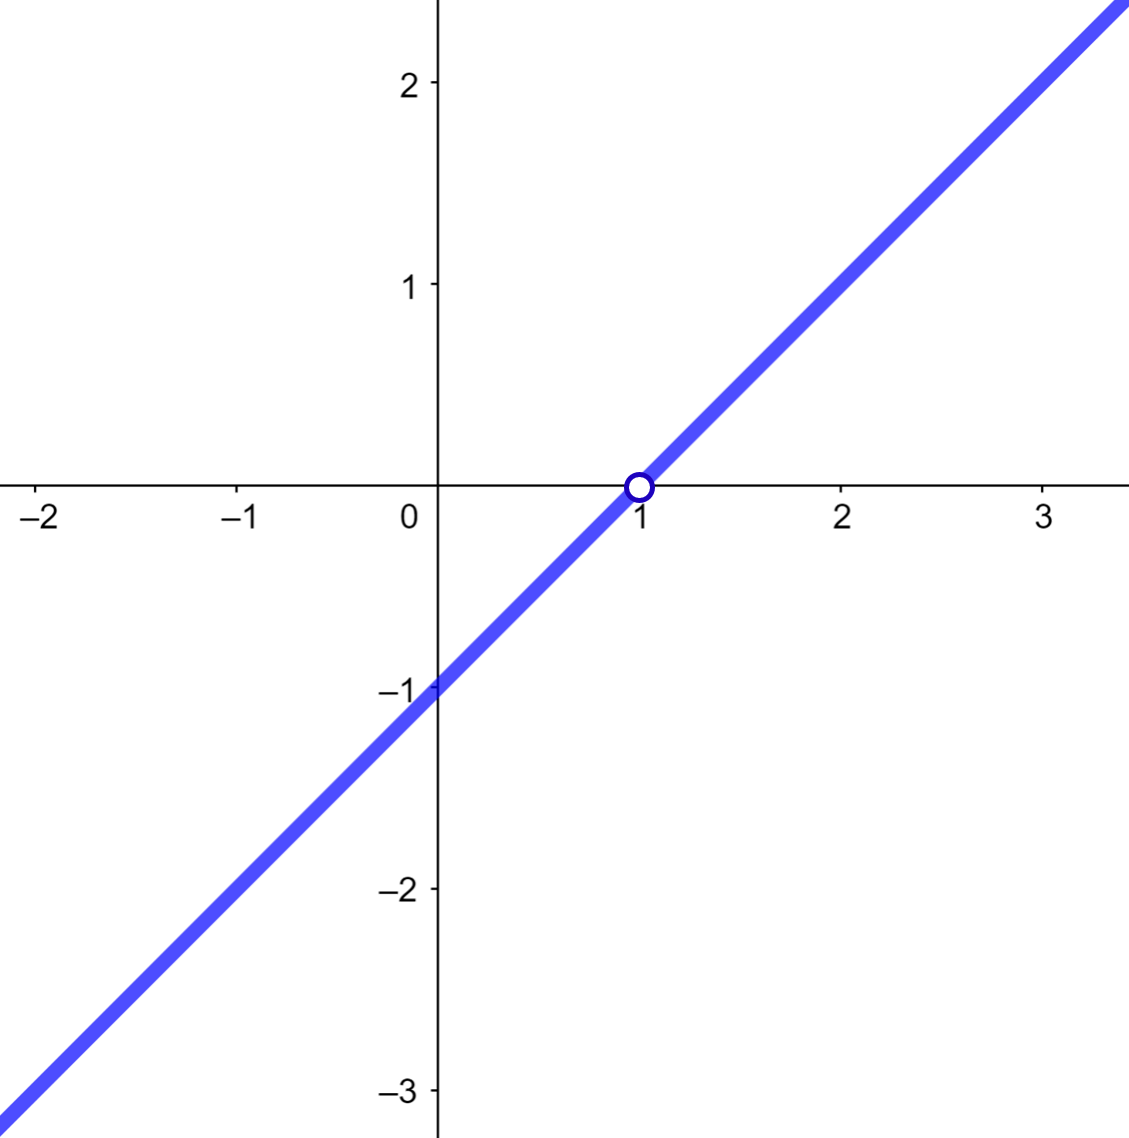
\includegraphics[width=\textwidth]{../Mathematik_1/Bilder/rationale_funktionen_gerade_hebbare_luecke.png}
\end{minipage}
	\begin{minipage}{0.6\textwidth}
		Das Bild zeigt den Graph der Funktion \[ f: x \mapsto \dfrac{p(x)}{q(x)}= \dfrac{ (x-1)^2}{(x-1)}\,.\]

		Den Funktionsverlauf von \(f\) analysieren wir wie folgt:
		\begin{itemize}
			\item Nullstellen des Z�hlers: \(N_p = \{1\}\).
			\item Nullstellen des Nenners: \(N_q = \{1\}\).
			\item Definitionsbereich von \(f\): \(D= \mathbb R\setminus \{ 1\} \)
			\item Nullstellen von $f$: \( N_f = \{\}\)!
			\item Polstellen von \(f\): \(P_f = \{\} \)
		\end{itemize}
		
\end{minipage}
\end{exabox}
		Die gebrochenrationale Funktion \(f\) besitzt eine Definitionsl�cke, keinen Pol und keine Nullstelle. Der Bruch ist nicht vollst�ndig gek�rzt -- die Funktionsabbildung kann noch vereinfacht werden:
		\[
			f: \mathbb R\setminus \{ 1\} \to \mathbb R\,, \dfrac{ (x-1)^2}{(x-1)} = x-1\,. 
\]

\noindent\textbf{Bemerkung:}
Beim K�rzen einer rationalen Funktion bleibt der urspr�ngliche Definitionsbereich erhalten. Eine durch K�rzen verschwundene Definitionsl�cke wird dadurch nicht zu einem Element des Definitionsbereichs.  

\subsection{Asymptoten f�r \(|x|\to\infty\)}

Das Verhalten einer rationalen Funktion f�r $x\to \pm\infty$ folgt grob aus dem Grad des Z�hlerpolynoms und dem Grad des Nennerpolynoms:

\begin{theorembox}{Asymptotisches Verhalten rationaler Funktionen}{ }

Es sei
\[
f(x)=\frac{p(x)}{q(x)}
\]
mit
\[
\deg(p)=n,
\qquad
\deg(q)=m.
\]

Dann gilt f�r \(|x|\to\infty\):

\begin{itemize}
	\item F�r \(n<m\) n�hert sich \(f(x)\) der horizontalen Asymptote \( y=0 \). 
	\item F�r \(n=m\) n�hert sich \(f(x)\) der horizontalen Asymptote \( y=\frac{a_n}{b_m}\), wobei \(a_n\) und \(b_m\) die f�hrenden Koeffizienten von Z�hler und Nenner sind.
    \item F�r \(n>m\) liefert die Polynomdivision
    \[
    f(x)=s(x)+\frac{r(x)}{q(x)},
    \qquad
    \deg(r)<\deg(q).
    \]
    Da
    \[
    \frac{r(x)}{q(x)}\to0
    \qquad\text{f�r}\qquad |x|\to\infty,
    \]
    beschreibt das Polynom \(s(x)\) das asymptotische Verhalten von \(f\).
\end{itemize}

\end{theorembox}

Im letzteren Fall kann man sogar noch genauer feststellen, wie die rationale Funktion gegen Unendlich geht: Sie schmiegt sich an die sogenannte Asymptote an, das ist der ganzrationale Anteil der \underline{Polynomdivision}\randverweis{MA1-polynome}.
\begin{exabox}{Asymptote f�r $x\to \pm\infty$}{ }\label{exa:asymptote}
	$\dfrac{x^3+4\cdot x^2 - 3\cdot x + 2}{ 2\cdot x-1} = \underbrace{ \frac12 \cdot x^2 + \frac94 \cdot x - \frac38}_{\displaystyle{\textnormal{Asymptote}}} + \underbrace{\displaystyle{\frac{\frac{13}{8}}{2\cdot x-1}}}_{ \displaystyle{\to 0}}\,. $
\end{exabox}

\noindent  \textbf{Bemerkungen:}\marginpar{Aufgaben}
\begin{itemize}
	\item Wenn das Z�hlerpolynom und das Nennerpolynom denselben Grad haben, dann schmiegt sich die Funktion an eine horizontale Gerade an. Man spricht auch von \textbf{horizontaler Asymptote}. 
	\item Wenn der Grad des Z�hlerpolynoms um eins gr��er ist als der des Nennerpolynoms, ergibt sich also eine \textbf{schr�ge Asymptotengerade}. Ist der Grad des Z�hlerpolynoms um zwei gr��er als der des Nennerpolynoms, ergibt sich eine quadratische Funktion wie in Beispiel \ref{exa:asymptote}.
	\item Hat eine gebrochenrationale Funktion eine Polstelle, so spricht man von einer \textbf{vertikalen Asymptote}. 
\end{itemize}

\begin{exabox}{Konstruktion einer gebrochenrationalen Funktion}{ }

Gesucht ist eine gebrochenrationale Funktion \(f\) mit folgenden Eigenschaften:
\begin{itemize}
    \item \(f\) besitzt bei \(x=-1\) eine doppelte Nullstelle,
    \item \(f\) besitzt bei \(x=2\) eine doppelte Polstelle,
    \item f�r \(|x|\to\infty\) n�hert sich \(f\) der horizontalen
          Asymptote \(y=3\).
\end{itemize}

Die doppelte Nullstelle bei \(x=-1\) f�hrt auf den Linearfaktor
\[
(x+1)^2
\]
im Z�hler. Damit ergibt sich zun�chst der Ansatz
\[
f(x)
=
a\cdot\frac{(x+1)^2}{(x-2)^2}.
\]

Der Faktor
\[
(x-2)^2
\]
im Nenner erzeugt bei \(x=2\) eine doppelte Polstelle. Da Z�hler und Nenner
denselben Grad besitzen, wird die horizontale Asymptote durch das Verh�ltnis
der f�hrenden Koeffizienten bestimmt. Es gilt
\[
\lim_{|x|\to\infty}
a\cdot\frac{(x+1)^2}{(x-2)^2}
=
a.
\]
Aus der geforderten horizontalen Asymptote \(y=3\) folgt daher
\[
a=3.
\]

Damit ergibt sich die gebrochenrationale Funktion
\[
	f:\mathbb R\setminus\{2\} \to \mathbb R, x \mapsto  
=
3\cdot\frac{(x+1)^2}{(x-2)^2}
\]

\end{exabox}
 \newpage % Rationale Funktoinen
\setcounter{exercise}{0} 
\ifintegriereaufgaben
\section*{Rationale Funktionen Aufgaben}\label{MA1-rationale-funktionen-aufgaben}

	Regeln und Beispiele, die zur Bearbeitung der Aufgaben hilfreich sind, finden Sie im Skript\wennreferenzvorhanden{MA1-rationale-funktionen}{ (Abschnitt \abschnittsverweis{MA1-rationale-funktionen})} und, falls Sie nicht weiterkommen, schauen Sie \hyperref[MA1-rationale-funktionen-loesungen]{hier}.
\else 
\section{Rationale Funktionen Aufgaben}\label{MA1-rationale-funktionen-aufgaben}

	Regeln und Beispiele, die zur Bearbeitung der Aufgaben hilfreich sind, finden Sie im Skript und, falls Sie nicht weiterkommen, schauen Sie \hyperref[MA1-rationale-funktionen-loesungen]{hier}.
\fi 


\begin{exercisebox}[Abbildungsvorschrift] %LS p186 -Aufgabe 4
	Geben Sie eine gebrochenrationale Funktion an mit 
	\begin{itemize}
		\item[(a)] Nullstelle $1$
		\item[(b)] Polstelle $3$ mit Vorzeichenwechsel
		\item[(c)] Polstelle $3$ ohne Vorzeichenwechsel
		\item[(d)] Nullstelle $1$ und Polstelle $3$ ohne Vorzeichenwechsel
		\item[(e)] Nullstellen $2$ und $3$, Polstelle $4$ mit Vorzeichenwechsel
		\item[(f)] Nullstelle $-1$, Polstelle $-3$ mit Vorzeichenwechsel, Polstelle $4$ ohne Vorzeichenwechsel
	\end{itemize}
\end{exercisebox}

\begin{exercisebox}[Asymptoten f�r \(|x|\to \infty\)] %p.31 Aufgabe 3  und b, c unter http://mathenexus.zum.de/html/analysis/funktionen_gebrochenrationale/weiterfuehrendes/gebro_04_Asys.htm  
		Untersuchen Sie das Verhalten der Funktion f�r $x\to \pm\infty$. Geben Sie gegebenenfalls die Gleichung der Asymptoten an.
	\begin{eqnarray*} \begin{array}{lll}
	(a)\; f(x)= \dfrac{7}{x} &\quad 
     %(b)\; f(x)= \dfrac{5}{3x-1} &\quad 
     %(c)\; f(x)= \dfrac{2}{x-2}-3 \\
     (b)\; f(x)= \dfrac{-3x^3+4x+16}{4x^2} &\quad 
     (c)\; f(x)= \dfrac{x^3+1}{x-1} \\
     (d)\; f(x)= \dfrac{2}{x}+\sqrt{x} &\quad 
     (e)\; f(x)= \dfrac{2}{(x-1)^2} &\quad 
     (f)\; f(x)= \dfrac{4}{\sqrt{x-2}} 
     \end{array}
     \end{eqnarray*}
    %\item $f(x)= 2- \frac{3}{\sqrt{x+3}}$
    %\item $f(x)= \frac{1}{x}+2\sin(x)$
\end{exercisebox}


%\begin{exercisebox}[Wolfram Alpha] %p31, Aufgabe 5 -- Pingo
%  Wie kann man mithilfe von Wolfram Alpha zu Vermutungen �ber den Grenzwert f�r $x\to\pm \infty$ gelangen? Geben Sie f�r $f$ solche Vermutungen an.
%  \begin{enumerate}
%    \item $f(x)= \frac{x}{2^x}$
%    \item $f(x)= \frac{x^2}{2^x}$
%    \item $f(x)= \frac{x^3}{1,5^x}$
%    \item $f(x)= \frac{x+2}{x^2-2}$
%    \item $f(x)= \frac{2x-1}{x+1}$
%    \item $f(x)= \frac{10\sin(x)}{x}$
%    \item $f(x)= 2^{-x} \cdot \sin(x)$
%    \item $f(x)= x^{\frac{1}{x}}, \; x>0$
%  \end{enumerate}
%\end{exercisebox}

\begin{exercisebox}[Vertikale Asymptoten] %p33, Aufgabe 6
  Untersuchen Sie das Verhalten von $f$ bei Ann�herung an die Definitionsl�cke. Geben Sie die Geichung der senkrechten Asymptote an.
	\begin{eqnarray*} \begin{array}{lll}
			(a)\; f(x) = \dfrac{2}{x} & \quad 
			(b)\; f(x) = -\dfrac{2}{x^2} &\quad 
			(c)\; f(x) = \dfrac{1}{x-4} \\[1ex]
			(d) \; f(x) = \dfrac{2}{4-x} &\quad 
     (e)\; f(x) = 1- \dfrac{1}{x} &\quad 
     (f) \; f(x) = \dfrac{3}{(x-1)^2} 
     \end{array}
     \end{eqnarray*}
\end{exercisebox}

\begin{exercisebox}[Asymptoten] % LS p. 189, Aufgabe 2
  Geben Sie die Gleichungen aller Asymptoten an
	\begin{eqnarray*} \begin{array}{lll}
			(a)\; f(x) = \dfrac{4}{3x^2} \quad \quad  & %a) 
	  (b)\; f(x) = \dfrac{2x+1}{x^2+3x} \quad\quad\quad & % f) 
	  (c)\; f(x) = \dfrac{x^4-x^2-1}{x^3-1} % p)
     \end{array}
  \end{eqnarray*}
\end{exercisebox}


\begin{exercisebox}[Qualitativer Graph] %LS p. 186 Aufgabe 2 a)-f)
	Ermitteln Sie von den folgenden Funktionen die 
	\begin{itemize}
		\item die Definitionsmenge,
		\item die Achsenabschnitte,
		\item die Nullstellen,
		\item die Polstellen inklusive der Analyse des Verhaltens von $f$ an jeder Polstelle und 
		\item fertigen Sie mit diesen Informationen eine qualitative Skizze des jeweiligen Funktionsgraphen an. 
	\end{itemize}
	\begin{eqnarray*} \begin{array}{lll}
			(a)\; f(x) = \frac{3x-1}{x-1} \quad & 
			(b)\; f(x) = \frac{x^2+x}{x+1} \quad & 
			(c)\; f(x) = \frac{x^2-9}{(x-3)^2} 
			%\\[1ex]
			%(d)\; f(x) = \dfrac{x^2-2x-15}{x-5} \quad &
     %(e)\; f(x) = \dfrac{3x-3}{x-1} \quad &
     %(f)\; f(x) = \dfrac{x^2+5x+2}{(x+1)^2} 
     \end{array}
  \end{eqnarray*}
\end{exercisebox}

%\begin{exercisebox}[Vermischte Aufgaben] -- Aufgabensammlung p. 38, Aufg. 8
%  Gegeben ist die Funktion $f$ mit $f(x) = \frac{1}{2(x+2)}+1$.
%  \begin{enumerate}
%    \item Bestimmen Sie die maximale Definitionsmenge von $f$.
%    \item Untersuchen Sie den Graphen von $f$ auf waagerechte und senkrechte Asymptoten.
%    \item Wo schneidet der Graph die $x$-Achse?
%    \item Skizzieren Sie den Graphen von $f$ mit seinen Asymptoten.
%    \item Entnehmen Sie der Sikzze eine Vermutung �ber die Symmetrie des Graphen. Beweisen Sie die Vermutung rechnerisch.
%  \end{enumerate}
%\end{exercisebox}

%\begin{exercisebox}[Asymptoten horizontal und vertikal] --> Aufgabensammlung p. 33, Aufg. 9
%  Gegeben ist die Funktion $f$ mit $f(x) = \frac{1}{(x+1)(x-2)}$
%  \begin{enumerate}
%    \item Geben Sie den maximalen Definitionsbereich der Funktion $f$ an.
%    \item Untersuchen Sie das Verhalten von $f$ bei Ann�herung an die Definitionsl�cken.
%    \item Untersuche Sie das Verhalten von $f$ f�r $x\to \pm \infty$
%    \item Skizzieren Sie den Graphen von $f$ mithilfe der Asymptoten.
%  \end{enumerate}
%\end{exercisebox}
 \newpage 
\setcounter{satz}{0} \setcounter{def}{0} \setcounter{exa}{0}  % Idee zur Herleitung (nach dem Prinzip: wir beherrschen nur Grundrechenarten): auswerten von 2^1, 2^2, 2^4, 2^5 - also 2^n als Funktion von n
\section{Exponentialfunktionen und Logarithmusfunktionen}\label{MA1-exponential-und-logarithmusfunktionen}

\begin{table}[H]
  \centering
  \begin{tabularx}{\textwidth}{p{0.9\textwidth} p{0.1\textwidth}}
    \toprule
	  \multicolumn{2}{c}{\textbf{�bersicht �ber Lernziele und Voraussetzungen}}\\
    \midrule
	  \textbf{Lernziele} &\\[.5\normalbaselineskip]
\tabitem Exponentialfunktionen und Logarithmusfunktionen erkennen und skizzieren &\\
\tabitem Definitionsbereich, Bildmenge und Monotonieverhalten von Exponential- und Logarithmusfunktionen beschreiben &\\
\tabitem Logarithmusfunktionen als Umkehrfunktionen von Exponentialfunktionen interpretieren &\\
\tabitem Rechenregeln f�r Exponential- und Logarithmusfunktionen anwenden &\\
\tabitem Gleichungen mit Exponential- und Logarithmusfunktionen l�sen &\\
\tabitem Logarithmen zu verschiedenen Basen ineinander umrechnen &\\
\tabitem logarithmische und doppelt logarithmische Darstellungen interpretieren &\\[.5\normalbaselineskip]
    \midrule
	  \textbf{Voraussetzungen}& \\[.5\normalbaselineskip]
	  \tabitem Grundlagen & \abschnittsverweis{MA1-mengen-und-logik}-\abschnittsverweis{MA1-aequivalenzumformungen}\\
	  \tabitem Injektivit�t, Bijektivit�t und Umkehrbarkeit & \abschnittsverweis{MA1-eigenschaften-von-funktionen}\\
	  \tabitem Potenzregeln & \abschnittsverweis{MA1-potenz-und-wurzelfunktionen}\\
	\tabitem algebraische Gleichungen & \abschnittsverweis{MA1-algebraische-gleichungen}\\
    \bottomrule
  \end{tabularx}
\end{table}

\ifintegriereaufgaben \noindent �bungsaufgaben zum Thema finden Sie hier: \hyperref[MA1-exponential-und-logarithmusfunktionen-aufgaben]{Aufgaben}
\vspace{0.3cm}
\hrule
 \fi

\subsection{Exponentialfunktionen}

Eine Funktion der Form
\[
f:\mathbb R\to(0,\infty),
\qquad
x\mapsto b^x,
\]
mit
\[
b>0,\qquad b\neq1,
\]
hei�t \textbf{Exponentialfunktion} (\emph{exponential function}).  Die Zahl \(b\) hei�t \textbf{Basis} (\emph{base}) der Exponentialfunktion.

Charakteristisch ist, dass die Variable \(x\) im Exponenten steht. Darin unterscheiden sich Exponentialfunktionen beispielsweise von Potenzfunktionen der Form 
\[
x\mapsto x^n,
\]
bei denen die Variable die Basis bildet.

Die Bedingung \(b>0\) stellt sicher, dass \(b^x\) f�r alle reellen Exponenten \(x\) definiert werden kann. F�r \(b=1\) entsteht die konstante Funktion
\[
x\mapsto1^x=1.
\]
Da hier kein Wachstum oder Zerfall vorliegt, wird \(b=1\) bei der Definition von Exponentialfunktionen ausgeschlossen.

\begin{theorembox}{Eigenschaften der Exponentialfunktionen}{ }
	\begin{minipage}{0.4\textwidth}
	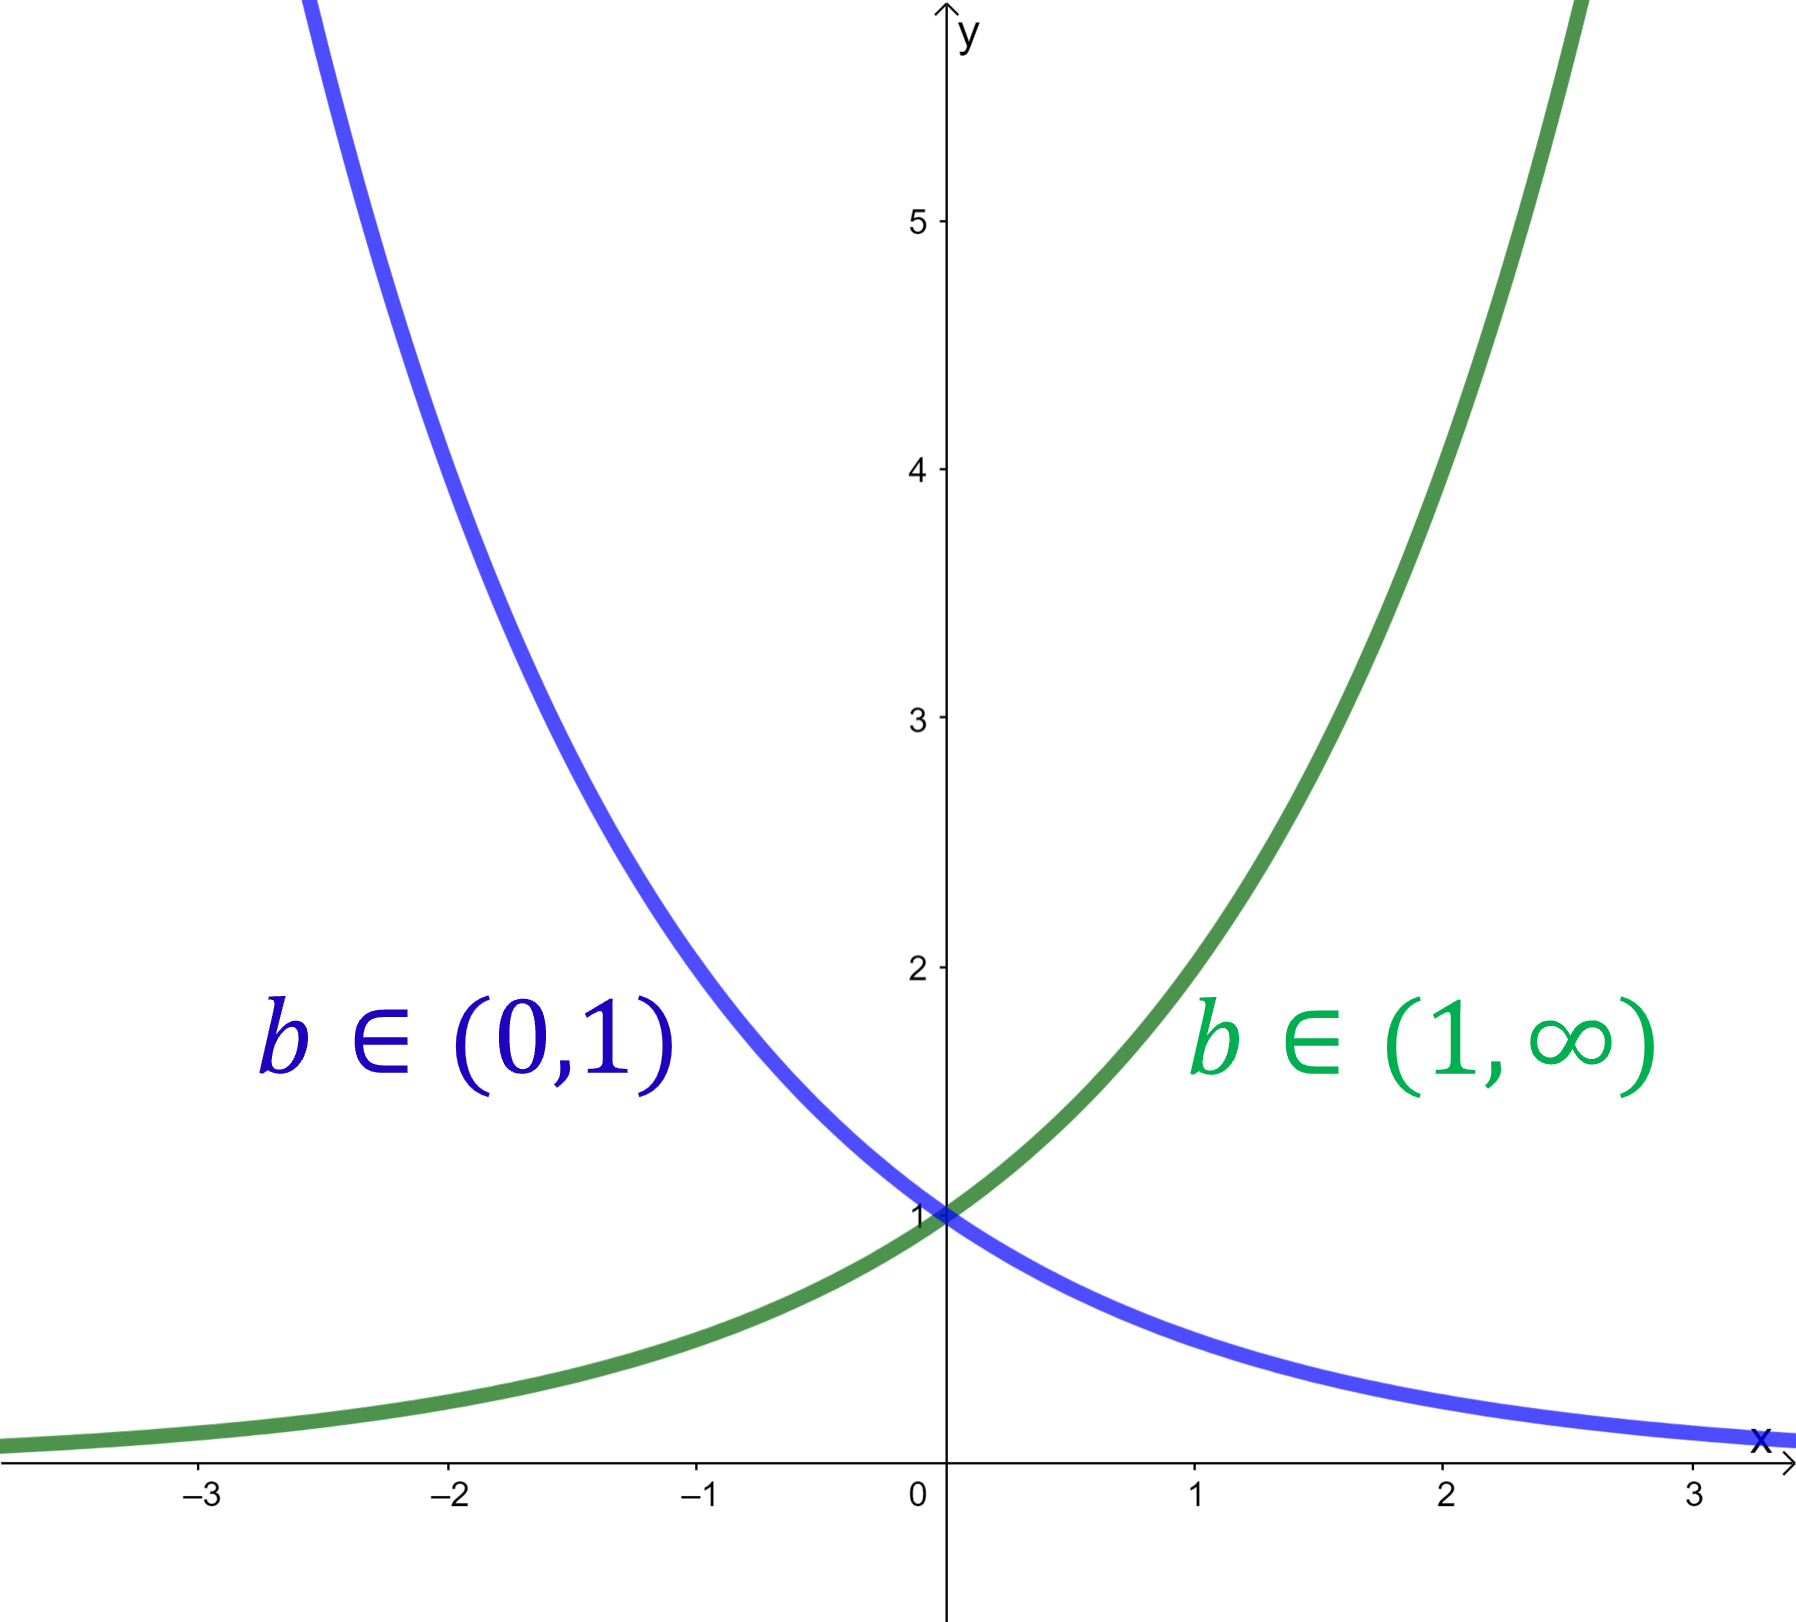
\includegraphics[width=\textwidth]{../Mathematik_1/Bilder/exponentialfunktionen_wachstum_zerfall.png}
\end{minipage}
	\begin{minipage}{0.6\textwidth}
		\begin{itemize}
			\item Definitionsbereich \(D = \mathbb R\). 
			\item Bildmenge $W = (0,\infty)$. 
			\item \(y\)-Achsenabschnitt an der Stelle $y = 1$. 
			\item \textcolor{darkgreen}{streng monoton steigend f�r \(b>1\)}.
			\item \textcolor{blue}{streng monoton fallend f�r \(0<b<1\)}.
		\end{itemize}
\end{minipage}
  
\end{theorembox}

Im vorigen Bild sieht man die Graphen der Funktionen 
\begin{eqnarray*}
	f: x &\mapsto &\textcolor{darkgreen}{2}^{\displaystyle x}\,,\\[2ex]
g: x&\mapsto &\left(\textcolor{blue}{\dfrac12}\right)^{\displaystyle x}\,.
\end{eqnarray*}
Die Graphen der Funktionen spiegeln sich an der \(y\)-Achse und das ist nicht �berraschend, denn 
$$ g(x) = \left(\frac1b\right)^x= b^{-x} = f(-x)\,.$$
F�r das Umformen von Gleichungen mit Exponentialfunktionen sind insbesondere die bereits bekannten Potenzregeln von Bedeutung.\marginpar{Aufgaben} 

\begin{theorembox}{Rechenregeln Exponentialfunktionen}{ }
	Es sei $b\in (0,1)\cup (1,\infty)$ und $x, y \in\mathbb R$. Betrachte die Funktion $x\mapsto b^x\,.$ Es gilt:
\begin{eqnarray*}
		b^0 &=& 1 \\
		b^{x+y} &=& b^x \cdot b^y\\
		b^{-x} &=& \displaystyle{\frac{1}{b^x}}\\ 
		\left( b^x \right)^y &=& b^{x\cdot y}
	\end{eqnarray*}
\end{theorembox}

\subsection{Die Exponentialfunktion $\exp: x\to e^x$}

Unter allen Exponentialfunktionen gibt es eine von besonderer Wichtigkeit. Es ist "\,die Exponentialfunktion"\, mit der Basis \(e\). \(e\) ist eine \textbf{irrationale Zahl} und das hei�t, dass wir Sie nie exakt als Dezimalzahl angeben k�nnen. Aber wir k�nnen sie approxmieren und hierf�r dient das folgende Experiment. Berechnen wir den Ausdruck
\begin{eqnarray*}
	(*) \quad a_n:= \left( 1+\frac1n\right)^n\,, 
\end{eqnarray*}
f�r ein paar $n \in \mathbb N$ aus, beispielsweise f�r $ n = 1,10,100,1000, 10000,100000 $: 

\begin{center}
	\begin{tabular}{c || c|c|c|c|c|c}
		$n$   & $1$ & $10$    & $100$   & $1000$  & $10000$ & $100000$ \\ \hline
	        $a_n$ & $2$ & $2,594$ & $2,705$ & $2,717$ & $2,718$ & $2,718$  
	\end{tabular}
\end{center}

Die Werte legen nahe, dass sich die Zahlen
\[
a_n=\left(1+\frac1n\right)^n
\]
f�r immer gr��ere \(n\) einer festen Zahl ann�hern. Diese Zahl hei�t \textbf{Eulersche Zahl} (\emph{Euler's number}) und wird mit \(e\) bezeichnet.

Mit dem sp�ter eingef�hrten Begriff des Grenzwerts l�sst sich dies schreiben als
\[
e
=
\lim_{n\to\infty}
\left(1+\frac1n\right)^n.
\]
Numerisch gilt
\[
e\approx2{,}718281828459\ldots
\]

Das Verhalten, das wir hier beobachtet haben, werden wir in Abschnitt \abschnittsverweis{MA1-lineare-gleichungssysteme} unter dem Begriff Folgenkonvergenz definieren.  Interessanterweise erhalten wir eine Darstellung f�r jedes Folgenglied \(a_n\) in \( (*)\) mit Hilfe des \underline{Binomischen Satzes}\randverweis{MA1-zahlenmengen}:
\[  
	\left( 1 + \displaystyle{\frac1n} \right)^n = \displaystyle{ \sum\limits_{k=0}^n} \binom{n}{k} \cdot \left( \displaystyle{\frac1n}\right)^k \cdot \left( 1\right)^{n-k} \,.
\]
Dies liefert eine alternative Approximation f�r die Eulersche Zahl, zum Beispiel f�r \(n=1000\):
  \begin{eqnarray*}
	  e = e^{\frac{1000}{1000}} &=& \left(e^{\frac{1}{1000}}\right)^{1000}  = \left(1,0010005\cdots\right)^{1000} \\ & \approx & \left( 1 + \frac{1}{1000}\right)^{1000} = \sum\limits_{k=0}^{1000} \binom{1000}{k} \cdot \frac{1}{1000^k} \\
		  & \approx & 1 + 1 + \frac{1}{2!}\frac{999}{1000}  + \frac{1}{3!}\frac{999\cdot 998}{1000\cdot 1000} + \frac{1}{4!}\frac{999\cdot 998\cdot 997}{1000\cdot 1000 \cdot 1000} + \cdots\\
		  & \approx & 1 + 1 + \frac{1}{2!}  + \frac{1}{3!} + \frac{1}{4!} + \cdots\,.
  \end{eqnarray*}

%Zwischen $2$ und $3$ wird also eine Zahl $e$ liegen, so dass $x\mapsto e^x$ an $x=0 $ genau in einem Winkel von $45^\circ$ steigt. Diese Zahl $e$ hei�t Eulersche Zahl [Euler�s number]. Die Funktion $x \mapsto e^x$ hei�t . 
%
%Aus der Eigenschaft $e\in(2,3)$ l��t sich eine n�herungsweise Berechnung von $e$ herleiten 
%  \begin{eqnarray*}
%    e = e^1 = e^{\frac{1}{1000}\cdot 1000} = \left( e^{\frac{1}{1000}}\right)^{1000}\; \Rightarrow \; e \approx \left( 1 +  \frac{1}{1000} \right)^{1000}\,.
%  \end{eqnarray*}

Dasselbe Prinzip legt f�r die Exponentialfunktion die Approximation
\[
e^x
\approx
\left(1+\frac{x}{n}\right)^n
\]
f�r gro�e \(n\) nahe. Mit dem \underline{binomischen Satz}\randverweis{MA1-zahlenmengen} ergibt sich
\[
\left(1+\frac{x}{n}\right)^n
=
\sum\limits_{k=0}^n
\binom nk\frac{x^k}{n^k}.
\]

F�r gro�e \(n\) n�hern sich die ersten Koeffizienten den Werten
\[
1,\quad 1,\quad \frac1{2!},\quad\frac1{3!},\quad\dots
\]
an. Dies deutet auf die sp�ter exakt zu begr�ndende Darstellung
\[
e^x
=
\sum\limits_{k=0}^{\infty}\frac{x^k}{k!}
=
1+x+\frac{x^2}{2!}+\frac{x^3}{3!}+\dots
\]
hin.

%Mit demselben Trick kann man die Exponentialfunktion $\exp: x\mapsto e^x$ f�r jedes \(x\in\mathbb R\) beliebig genau berechnen, ohne jemals krumme Potenzen zu bilden:
%\begin{eqnarray*}
%	e^x & \approx & \left( 1 + \frac{x}{1000}\right)^{1000} =  \sum\limits_{k=0}^{1000} \binom{1000}{k} \cdot \frac{x}{1000^k}\\
%& \approx & 1 + x + \frac{x^2}{2!}\frac{999}{1000}  + \frac{x^3}{3!}\frac{999\cdot 998}{1000\cdot 1000} + \frac{x^4}{4!}\frac{999\cdot 998\cdot 997}{1000\cdot 1000 \cdot 1000} + \cdots\\
%  &\approx&  1 + x + \frac{1}{2!}x^2 + \frac{1}{3!}x^3 + \frac{1}{4!}x^4 \cdots \,.
%\end{eqnarray*}

%Man kann zeigen, dass die obigen Approximationen f�r \(n\to\infty\) tats�chlich die Eulersche Zahl bzw. die Exponentialfunktion darstellen:\footnote{Um das zu beweisen fehlt uns im Moment das Handwerkszeug.}
%	\[ \begin{array}{rcl}
%		e  &=& \displaystyle{ \sum\limits_{k=0}^\infty} \displaystyle{\frac{1}{k!}}\,,\\
%	e^x  &=& \displaystyle{\sum\limits_{k=0}^\infty}\displaystyle{ \frac{x^k}{k!}}\,. \end{array}
%\]

Die Exponentialfunktionen beschreiben Wachstums- oder Zerfallsprozesse. 
\begin{itemize} 
	\item Die Zinsen werden hier einem Kapital \(K\) �ber einen gewissen Zeitraum zugeschlagen und mit verzinst. Dies f�hrt zu exponentiellem Wachstum des Kapitals. Die Zinseszinsformel lautet: $$K(t) = K(0)\cdot \left(1+\displaystyle{\frac{p}{100}}\right)^t\,,$$ wobei \(p\) die Zinszahl und \(K(0)\) das Anfangskapital darstellt. Bei einem Sparbuch mit \(5\%\) Zinsen pro Jahr hat sich Anfangskapital nach ca. \(14\) Jahren verdoppelt: $$ K(14) = K(0)\cdot \left(1+\displaystyle{\frac{5}{100}}\right)^{14} \approx 1,98\cdot K(0)\,.$$
	\item Das Zerfallsgesetz ist die in der Physik �bliche Bezeichnung der Gleichung, die eine exponentielle zeitliche Abnahme von Gr��en beschreibt. In der Kernphysik gibt das Zerfallsgesetz die Anzahl \(N\) der zu einem Zeitpunkt \(t\) noch nicht zerfallenen Atomkerne einer radioaktiven Substanzprobe an. Diese Anzahl betr�gt $$ N(t) = N(0)\cdot e^{-\lambda t}\,, $$ wobei \(N(0)\) die Anzahl der zum Zeitpunkt \(t=0\) vorhandenen Atomkerne und \(\lambda\) die Zerfallsrate des betreffenden Nuklids ist.
%\item In der Thermodynamik betrachtet man h�ufig Verteilungen von Teilchen auf Niveaus verschiedener Energie $E$. Sind quantenmechanische Effekte egal und ist die Zahl der Teilchen fest und ist die Gesamtenergie fest und ist die Unordnung (Entropie) maximal, ist das Energieniveau $E$ proportional zu $e^{-E/kT}$ besetzt. Dazu kommen noch weitere Faktoren, zum Beispiel, um die Zustandsdichten zu ber�cksichtigen. Dabei ist $k$ die Boltzmann-Konstante, 
%	$$ k = 1,380649 \dot 10^{-23} \mathrm{J}/\mathrm{K}\,.$$ 
%	Diese Verteilung schl�gt sich an vielen Stellen nieder. Die Arrhenius-Gleichung modelliert, wie eine Reaktionsgeschwindigkeit \(v_{\mathrm{reac}}\) von der Temperatur abh�ngt:
%	\begin{exabox}{Arrhenius-Gleichung}{ }
%	$ v_{\mathrm{reac}} \approx e^{-\frac{E}{R\dot T}}\,,$
%\end{exabox}
%wobei \( R=N\cdot k\) die universelle Gaskonstante bezeichnet.  
%\item In  der  Halbleiterdiode  wirkt  die  Raumladungszone  am  $pn$-�bergang  wie  die Aktivierungsenergie in einer chemischen Reaktion. Die ben�tigte Energie wird durch eine in Durchlassrichtung angelegte Spannung $U$ vermindert. Das �bliche Modell f�r kleine Str�me durch eine Diode ist damit:
%
%
%Was sind offensichtlichen Grenzen dieses Modells?
\end{itemize}

\subsection{Logarithmusfunktionen}

Da die Exponentialfunktion
\[
f:\mathbb R\to(0,\infty),
\qquad
x\mapsto b^x,
\]
f�r \(b>0\) und \(b\neq1\) streng monoton und damit bijektiv ist, besitzt sie
eine \underline{Umkehrfunktion}\randverweis{MA1-eigenschaften-von-funktionen}.

Diese Umkehrfunktion hei�t \textbf{Logarithmusfunktion}
(\emph{logarithmic function}) zur Basis \(b\):
\[
\log_b:(0,\infty)\to\mathbb R.
\]

Dabei gilt
\[
y=b^x
\qquad\Longleftrightarrow\qquad
x=\log_b(y).
\]

\noindent{\textbf{Merke:}} 
\begin{itemize}
        \item Ein Logarithmus beantwortet die Frage: Womit muss man die Basis $b$ potenzieren, damit $y$ herauskommt? 
        \item Eine Exponentialfunktion bildet nur auf positive Zahlen ab, also k�nnen Logarithmusfunktionen nur positive Zahlen verarbeiten. 
\end{itemize}

Einige Logarithmusfunktionen sind besonders wichtig und haben deshalb spezielle Bezeichnungen:
\begin{defbox}{Bezeichnungen wichtiger Logarithmusfunktionen}{ }
  \begin{enumerate}
    \item Den Logarithmus zur Basis $e$ schreibt man $\ln:= \log_e$ und nennt ihn den nat�rlichen Logarithmus,
    \item Den Logarithmus zur Basis $10$ schreibt man $\mathrm{lg}:= \log_{10}$,
    \item Den Logarithmus zur Basis $2$ schreibt man $\mathrm{lb}:= \log_2$.
  \end{enumerate}
\end{defbox}

\noindent{\textbf{Vorsicht:}} In Programmiersprachen und in der fortgeschrittenen Mathematik hei�t der nat�rliche Logarithmus oft $\log$. 

Exponentialfunktionen wachsen f�r Basen \(b>1\) sehr schnell, w�hrend Logarithmusfunktionen nur sehr langsam wachsen. Anschaulich gesprochen: Exponentialfunktionen �explodieren�, Logarithmusfunktionen �kriechen�.  Trotz dieses langsamen Wachstums ist die Logarithmusfunktion nach oben unbeschr�nkt.
\begin{exabox}{Monotonie des Logarithmus - es kriecht}{ }
	\begin{minipage}{0.7\textwidth}
	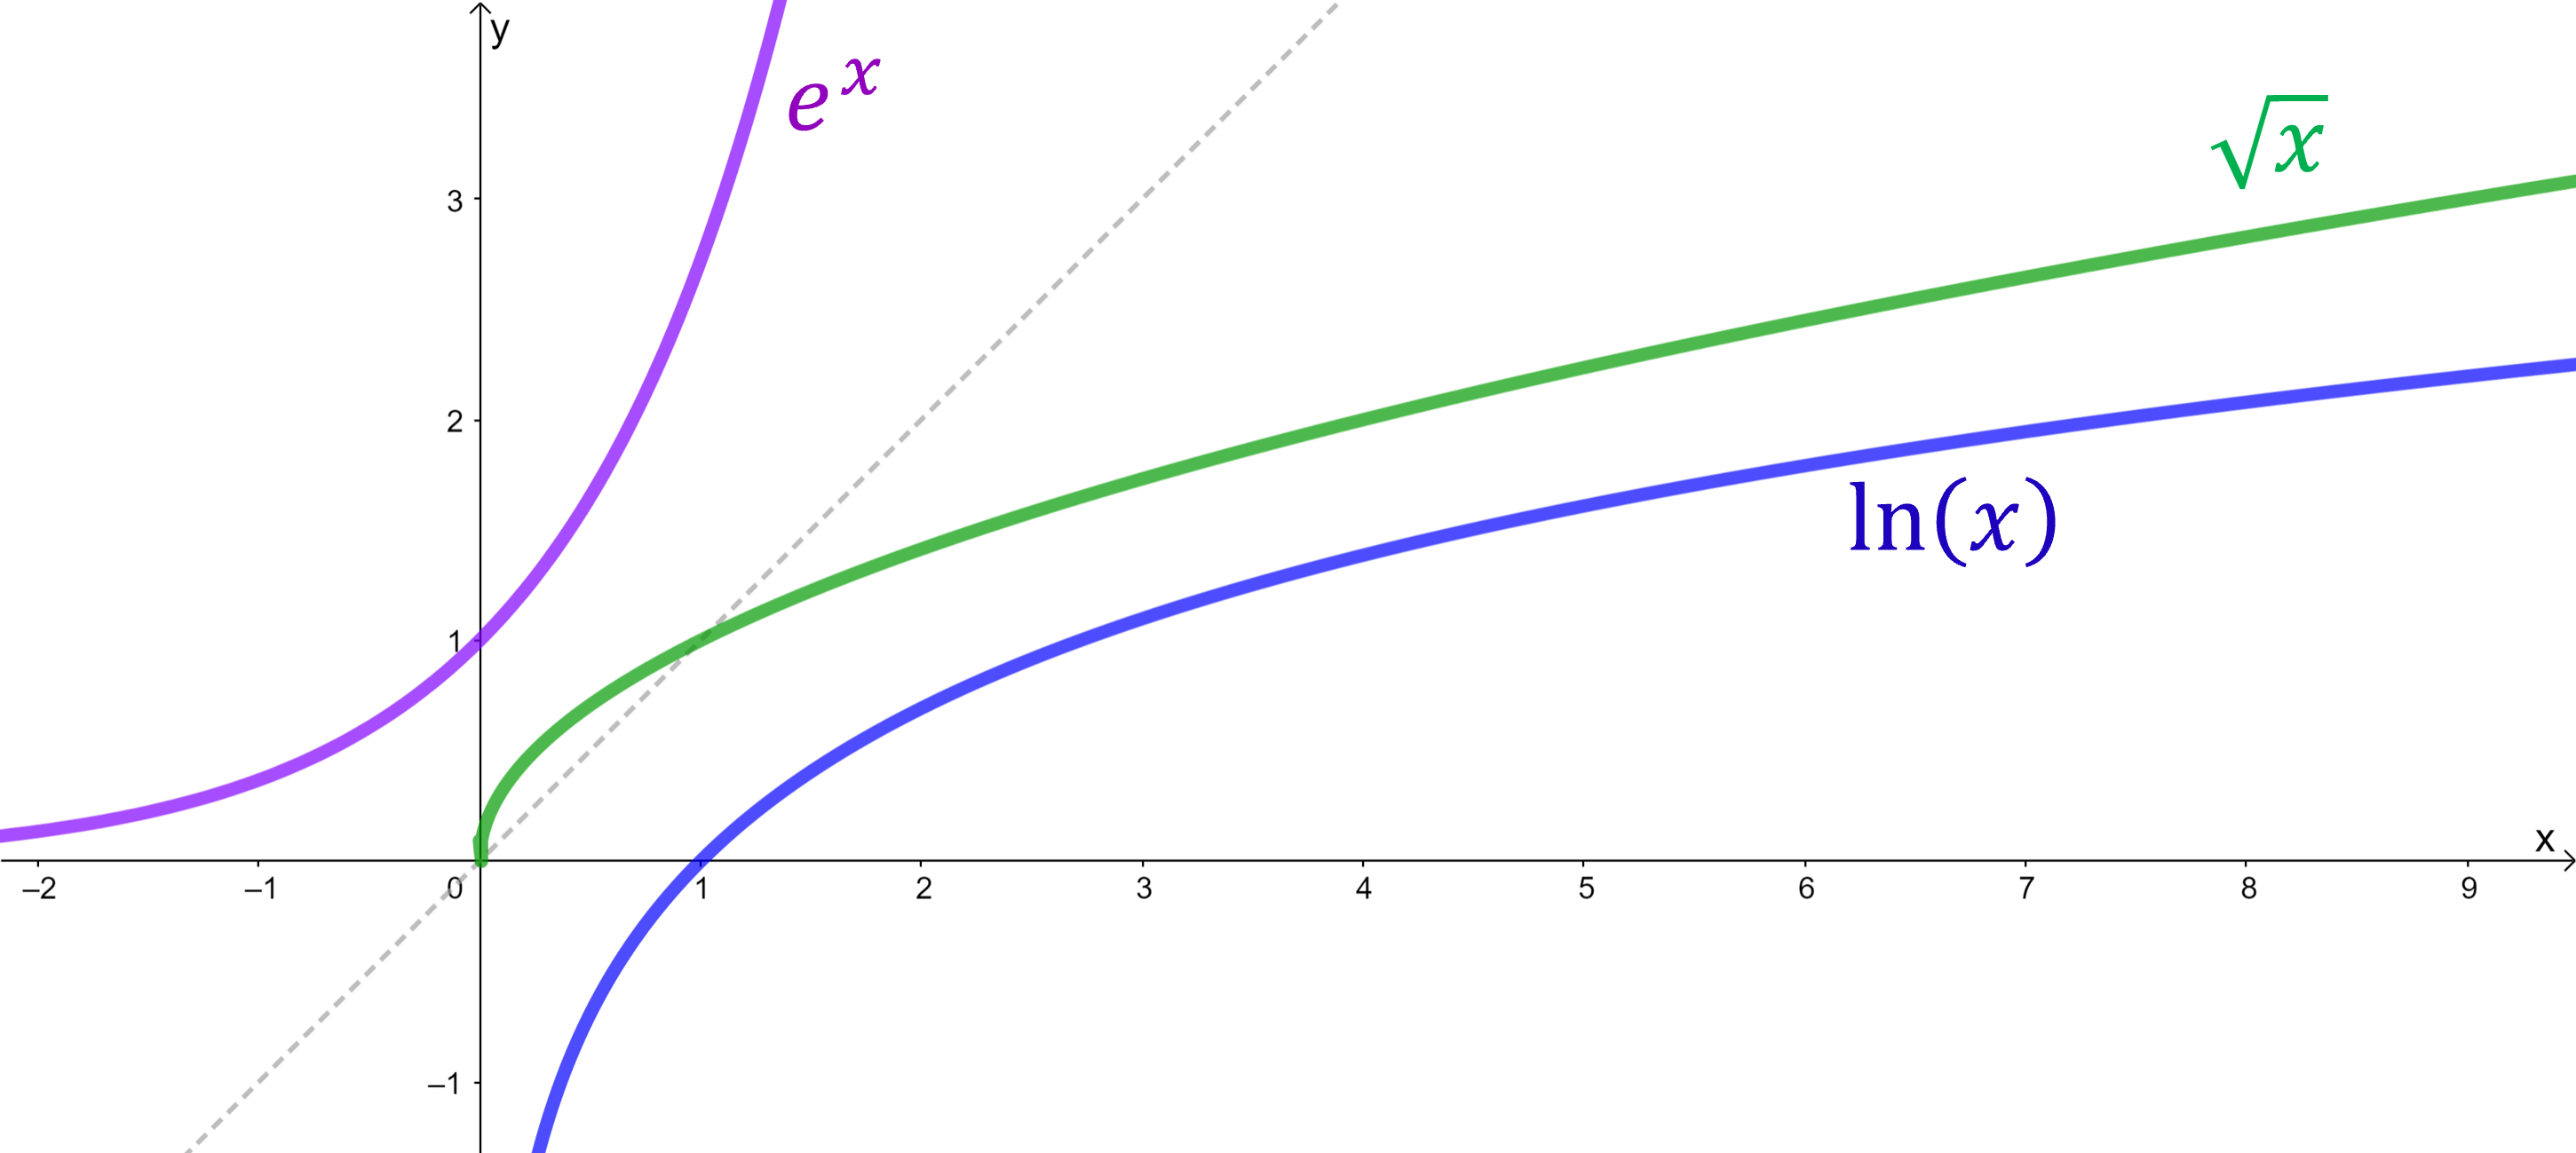
\includegraphics[width=\textwidth]{../Mathematik_1/Bilder/logarithmus_wachstumsvergleich_exponentialfunktion_quadratwurzel.png}
\end{minipage}
	\begin{minipage}{0.3\textwidth}
		\begin{itemize} 
			\item \textcolor{violett}{Exponentialfunktion} 
			\item \textcolor{darkgreen}{Quadratwurzel}
			\item \textcolor{blue}{Logarithmusfunktion}
		\end{itemize}
\end{minipage}
\end{exabox}

Weil die Logarithmusfunktionen die jeweiligen Exponentialfunktionen umkehren, kann  man  aus  den  Potenzrechengesetzen  die  Rechenregeln  f�r  Logarithmusfunktionen folgern:\marginpar{Aufgaben}
\begin{theorembox}{Rechenregeln Logarithmusfunktionen}{ }
	F�r alle $x,y > 0$, $b>0$, $b\not=1$, $z\in \mathbb R$ gilt:
  \begin{eqnarray*}
    \log_b(x\cdot y) &=& \log_b(x) + \log_b(y)\\ 
    \log_b\left(\displaystyle{\frac{x}{y}}\right) &=& \log_b(x) - \log_b(y)\\ 
    \log_b\left(x^z\right) &=&  z\log_b(x)\\ 
    \log_b\left(\sqrt[n]{x}\right) &=&  \displaystyle{\frac1n} \log_b(x), \quad n\in \mathbb N^+\,.
  \end{eqnarray*}
\end{theorembox}

Oft sind am Rechner nur $\mathrm{lg}$ und $\ln$ verf�gbar, keine Logarithmusfunktion zubeliebigen Basen $b$. Dann kann man sich so behelfen: $x=\log_3(7)$, also $7=3^x$, also:
\begin{exabox}{$x=\log_3(7)$}{ }
  $
  \left. \begin{array}{rcl} 7 &=& 10^{\mathrm{lg}(7)}\\
3^x &=& \left( 10^{\mathrm{lg}(3)}\right)^x
\end{array} \right\} \quad \Rightarrow \; \mathrm{lg}(7) = x\cdot \mathrm{lg}(3)  \; \Rightarrow \;  x = \displaystyle{\frac{\mathrm{lg}(7)}{\mathrm{lg}(3)}}\,.
$
\end{exabox}

\begin{theorembox}{Basiswechsel}{ }
	Es gilt 
	\[ \log_b(x) = \dfrac{\log_a(x)}{\log_a(b)} \] 
	f�r alle \(a>0\), \(a\not =1\) und damit insbesondere f�r \(a=e\)
	\[ \log_b(x) = \dfrac{\ln(x)}{\ln(b)} \] 

\end{theorembox}

Auch die Logarithmusfunktionen kommen auf nat�rliche Weise vor:

\begin{itemize}
	\item Schallpegel werden aufgrund der sehr gro�en auftretenden Wertebereiche logarithmisch angegeben. Der Schalldruckpegel ist beispielsweise durch 
		\[ 
			L_p = 20\lg\left(\frac{p}{p_0}\right)\,\mathrm{dB}, \qquad p_0=20\,\mu\mathrm{Pa},
\]
definiert.
\item Au�erdem verh�lt sich der Informationsgehalt logarithmisch:
  $$ \mathrm{lb}\left( \textnormal{Anzahl der Zust\"ande} \right) \; \mathrm{Bits}\,.$$
Zum Beispiel kann man die Zahlen von $0$ bis $255$ in $8$ Bits (Ja-Nein Informationen) speichern.  
\end{itemize}

\begin{exabox}{Gleichungen mit Exponential- und Logarithmusfunktionen}{ }

\textbf{1. Exponentialgleichung}

Gegeben sei die Gleichung
\[
3^{2\cdot x-1}=7.
\]
Die Unbekannte \(x\) steht im Exponenten. Da sich beide Seiten nicht als
Potenzen derselben Basis darstellen lassen, wird die Gleichung logarithmiert:
\[
	\begin{array}{c rcl l}
	& 3^{2\cdot x-1}&=& 7 &\quad\quad \big\|\,\ln(\cdot )\\
\Leftrightarrow\quad  & \ln\left(3^{2\cdot x-1}\right)&=&\ln(7) &\quad\quad \big\|\,\text{Logarithmengesetz anwenden}\\
\Leftrightarrow\quad  & (2\cdot x-1)\ln(3)&=&\ln(7) &\quad\quad \big\|\,\text{vereinfachen}\\
\Leftrightarrow\quad  & 2\cdot x-1&=&\frac{\ln(7)}{\ln(3)} &\quad\quad \big\|\,+1\\
\Leftrightarrow\quad  & 2x&=&1+\frac{\ln(7)}{\ln(3)} &\quad\quad \big\|\, :2\\
\Leftrightarrow\quad  & x&=&\frac12\left(1+\frac{\ln(7)}{\ln(3)}\right). &
\end{array}
\]
Damit lautet die L�sungsmenge \( \mathbb L = \left\{ \frac12\left(1+\frac{\ln(7)}{\ln(3)}\right) \right\}\).

\noindent{\textbf{Fazit:}} Das Logarithmieren erm�glicht hier, den Exponenten mithilfe der Regel \( \ln(a^z)=z\ln(a) \) aus der Potenz herauszul�sen. Die Exponentialgleichung wird dadurch auf eine lineare Gleichung zur�ckgef�hrt.

\bigskip
\textbf{2. Logarithmusgleichung}

Gegeben sei die Gleichung
\[
\ln(x-1)+\ln(x+1)=\ln(8)
\]
Bevor die Gleichung umgeformt wird, muss ihr Definitionsbereich bestimmt
werden. Die Argumente der Logarithmen m�ssen positiv sein: 
\[
x-1>0
\qquad\text{und}\qquad
x+1>0.
\]
Beide Bedingungen sind genau dann erf�llt, wenn \(x>1\).
Damit gilt \( D=(1,\infty) \).  
Innerhalb dieses Definitionsbereichs k�nnen die Logarithmusregeln angewendet
werden:
\[
	\begin{array}{c rcl l}
	& \ln(x-1)+\ln(x+1) &=& \ln(8) &\quad \| \,\text{Logarithmengesetz anwenden}\\
	\Leftrightarrow \quad & \ln\bigl((x-1)(x+1)\bigr) &=& \ln(8) &\quad \| \exp(\cdot ) \\
	\Leftrightarrow \quad & (x-1)(x+1) &=8 &\quad \| \, \text{Eigenschaft Umkehrfunktion} \\ 
	\Leftrightarrow \quad & x^2 &=& 9 &\quad \| \sqrt{\cdot } \\
\Leftrightarrow \quad & |x| &=3.&
\end{array}
\]

Die algebraische Gleichung besitzt damit zun�chst die beiden L�sungen \(x=-3\) und \(x=3\).  F�r die urspr�ngliche Logarithmusgleichung muss jedoch zus�tzlich der Definitionsbereich \( x>1\) ber�cksichtigt werden. Daher entf�llt \(x=-3\), und es bleibt \(\mathbb L=\{3\}\).

\noindent{\textbf{Fazit:}} Eine Logarithmusgleichung kann durch die Logarithmusregeln auf eine algebraische Gleichung zur�ckgef�hrt werden.  Die L�sungen der algebraischen Gleichung sind anschlie�end mit dem Definitionsbereich der urspr�nglichen Gleichung abzugleichen.

\end{exabox}


\subsection{Logarithmische Darstellung}

Exponentialfunktionen und Potenzfunktionen k�nnen sich �ber gro�e Wertebereiche
erstrecken. In einer gew�hnlichen linearen Darstellung sind kleine
Funktionswerte dann h�ufig kaum noch zu erkennen, w�hrend gro�e Funktionswerte
den Graphen dominieren.

Eine logarithmische Skalierung der Achsen erm�glicht nicht nur eine
�bersichtlichere Darstellung solcher Wertebereiche. Sie besitzt au�erdem eine
wichtige mathematische Eigenschaft: Bestimmte nichtlineare Zusammenh�nge
erscheinen bei geeigneter logarithmischer Darstellung als Geraden. Dadurch
k�nnen exponentielle Zusammenh�nge und Potenzgesetze in Messdaten leichter
erkannt und untersucht werden.

\subsubsection*{Exponentielle Zusammenh�nge}

Es sei ein exponentieller Zusammenhang der Form
\[
y=C\cdot b^x,
\qquad
C>0,\quad b>0,\quad b\neq1,
\]
gegeben. Durch Logarithmieren folgt
\[
\begin{aligned}
y&=C\cdot b^x\\
\Longrightarrow\qquad
\ln(y)
&=\ln\left(C\cdot b^x\right)\\
&=\ln(C)+\ln\left(b^x\right)\\
&=\ln(C)+x\ln(b).
\end{aligned}
\]

Damit besteht zwischen \(x\) und \(\ln(y)\) ein linearer Zusammenhang:
\[
\ln(y)=\ln(C)+\ln(b)\cdot x.
\]

Wird also die \(x\)-Achse linear und die \(y\)-Achse logarithmisch skaliert,
erscheint der Graph eines exponentiellen Zusammenhangs als Gerade. Eine solche
Darstellung hei�t \textbf{halblogarithmische Darstellung}
(\emph{semi-logarithmic plot}).

Aus der Geraden lassen sich die Parameter der Exponentialfunktion ablesen:
Der Achsenabschnitt entspricht \(\ln(C)\), die Steigung entspricht
\(\ln(b)\).

\begin{exabox}{Exponentieller Zusammenhang in halblogarithmischer Darstellung}{ }

F�r
\[
y=5\cdot 2^x
\]
ergibt das Logarithmieren
\[
\begin{aligned}
\ln(y)
&=\ln\left(5\cdot2^x\right)\\
&=\ln(5)+x\ln(2).
\end{aligned}
\]
In einer Darstellung von \(\ln(y)\) gegen \(x\) entsteht daher eine Gerade
mit dem Achsenabschnitt
\[
\ln(5)
\]
und der Steigung
\[
\ln(2).
\]

Ein exponentieller Zusammenhang, der in einer gew�hnlichen Darstellung
gekr�mmt erscheint, wird durch das Logarithmieren der \(y\)-Werte also
linearisiert.

\end{exabox}

\subsubsection*{Potenzgesetze}

Ein �hnlicher Zusammenhang entsteht bei Potenzfunktionen. Es sei
\[
y=C\cdot x^\alpha,
\qquad
C>0,\quad x>0.
\]
Durch Logarithmieren folgt
\[
\begin{aligned}
y&=C\cdot x^\alpha\\
\Longrightarrow\qquad
\ln(y)
&=\ln\left(C\cdot x^\alpha\right)\\
&=\ln(C)+\ln\left(x^\alpha\right)\\
&=\ln(C)+\alpha\ln(x).
\end{aligned}
\]

Damit besteht zwischen \(\ln(x)\) und \(\ln(y)\) wiederum ein linearer
Zusammenhang:
\[
\ln(y)=\ln(C)+\alpha\ln(x).
\]

Werden sowohl die \(x\)-Achse als auch die \(y\)-Achse logarithmisch skaliert,
erscheint ein Potenzgesetz als Gerade. Eine solche Darstellung hei�t
\textbf{doppelt logarithmische Darstellung}
(\emph{log-log plot}).

Die Steigung dieser Geraden entspricht unmittelbar dem Exponenten
\(\alpha\). Der Achsenabschnitt entspricht \(\ln(C)\).

\begin{exabox}{Doppelt logarithmische Darstellung}{ }

F�r den Zusammenhang
\[
y=2x^2
\]
gilt
\[
\begin{aligned}
\ln(y)
&=\ln(2x^2)\\
&=\ln(2)+2\ln(x).
\end{aligned}
\]
In einer doppelt logarithmischen Darstellung entsteht daher eine Gerade mit
der Steigung
\[
2.
\]
Der Exponent des Potenzgesetzes kann somit unmittelbar aus der Steigung der
Geraden bestimmt werden.

\medskip
\centering
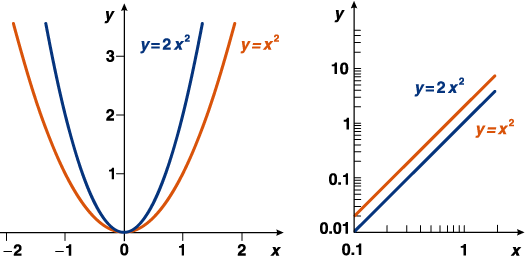
\includegraphics[width=0.6\textwidth]
{../Mathematik_1/Bilder/logarithmische_darstellung_potenzgesetze.png}

\end{exabox}
 \newpage % Exponentialfunktoinen und Logarithmen
\setcounter{exercise}{0} 
\ifintegriereaufgaben
\section*{Exponential- und Logarithmusfunktionen Aufgaben}\label{MA1-exponential-und-logarithmusfunktionen-aufgaben}

	Regeln und Beispiele, die zur Bearbeitung der Aufgaben hilfreich sind, finden Sie im Skript\wennreferenzvorhanden{MA1-exponential-und-logarithmusfunktionen}{ (Abschnitt \abschnittsverweis{MA1-exponential-und-logarithmusfunktionen})} und, falls Sie nicht weiterkommen, schauen Sie \hyperref[MA1-exponential-und-logarithmusfunktionen-loesungen]{hier}.
\else 
\section{Exponential- und Logarithmusfunktionen Aufgaben}\label{MA1-exponential-und-logarithmusfunktionen-aufgaben}

	Regeln und Beispiele, die zur Bearbeitung der Aufgaben hilfreich sind, finden Sie im Skript und, falls Sie nicht weiterkommen, schauen Sie \hyperref[MA1-exponential-und-logarithmusfunktionen-loesungen]{hier}.
\fi 

\begin{exercisebox}[Interpolation]
	Bestimmen Sie die Parameter $a$ und $b$ der Funktion \[ f:x\mapsto a\cdot e^{-bx}\] so, dass die Punkt $(0|8)$ und $(5|3)$ auf der Kurve liegen. Runden Sie die Parameter auf drei Nachkommastellen.
\end{exercisebox}

\begin{exercisebox}[$f: x\mapsto 2^x$]
  Gegeben ist die Funktion $f$ mit $f: x \mapsto 2^x$
  \begin{itemize}
	  \item[(a)] Ermitteln Sie den maximalen Definitionsbereich $D$ und die Bildmenge $f(D)$
	  \item[(b)] Berechnen Sie $f(-\frac14)$ auf $2$ Dezimalen genau.
    \item[(c)] F�r welches $x\in D$ ist $f(x) = 8$?
    \item[(d)] F�r welche $x\in D$ ist $f(x) \leq 16$?
    \item[(e)] Zeigen Sie $f(x) \cdot f(-x) = 1$ f�r alle $x\in D$
    \item[(f)] Zeigen Sie $f(x+1) = 2\cdot f(x)$ f�r alle $x\in D$
  \end{itemize}
\end{exercisebox}

\begin{exercisebox}[Rechenregeln]
	\begin{itemize}
		\item[(a)] Vereinfachen Sie die folgenden Ausdr�cke ohne Taschenrechner:
			\[ \mathrm{lg}(4)+2\mathrm{lg}(5), \; e^{5\ln(2)}, \; \mathrm{lg}(3000)- \mathrm{lg}(3)\,.\]
		\item[(b)] In folgender Umformung ist ein Fehler - finden Sie ihn?
			\[ e^{0.5(\ln x )^2} = \left( e^{(\ln x)^2}\right)^{0.5} = e^{(\ln x)^{2\cdot 0.5}} = e^{(\ln x)} =  x\,.\]
	\end{itemize}
\end{exercisebox}

\begin{exercisebox}[Gleichungen]
	L�sen Sie die folgenden Gleichungen:
	\begin{eqnarray*}
		\begin{array}{ll} 
			(a)\; \displaystyle{e^{x^2 - 2x}}=1 \quad & (b)\; e^x+2\cdot e^{-x} = 3 \\ (c)\; \ln\left( \sqrt{x}\right) + 1,5\cdot \ln(x) = \ln(2x) \quad &(d)\; \left( \mathrm{lg}(x)\right)^2 - \mathrm{lg}(x) = 2 
		\end{array}
	\end{eqnarray*}
\end{exercisebox}

\begin{exercisebox}[Anwendung: Radioaktiver Zerfall]
	Eine radioaktive Substanz zerf�llt nach dem Gesetz \[ n(t) = n_0 \cdot e^{-\lambda t} \,.\]
	mit $n_0, \lambda \in \mathbb R^+$. Die halbwertszeit $\tau$ ist definiert durch $n(\tau) = n(0)/2$. 
	\begin{itemize}
		\item[(a)] Bestimmen Sie die Umkehrfunktion mit Definitionsbereich, Wertebereich und Abbildungsvorschrift. 
		\item[(b)] Geben Sie eine allgemeine Formel f�r $\tau$ an. 
		\item[(c)] Berechnen Sie die Halbwertszeitf�r Radon mit $\lambda = 2,0974\cdot 10^{-6}s^{-1}\,.$
	\end{itemize}
\end{exercisebox}

%\begin{exercisebox}[Logarithmische Skalen]
%\end{exercisebox}
%
%\begin{exercisebox}[Approximation von $e$ Taylorentwicklung, Matlab]
%\end{exercisebox}
%
%\begin{exercisebox}[Approximation von $\pi$, Monte-Carlo Verfahren, Matlab]
%\end{exercisebox}

%
%\begin{exercisebox}[Numerische Verfahren analysieren]
%optimale Konvergenz, Logarithmische Konvergenz $n\log(n)$, Quasi-Linear
%\end{exercisebox}
%
%\begin{exercisebox}[Gleichverteilte Zufallszahlen]
%\end{exercisebox}
%
%\begin{exercisebox}[Exponentialverteilung, Zufallszahlen Modellierung]
%\end{exercisebox}
 \newpage 
\setcounter{satz}{0} \setcounter{def}{0} \setcounter{exa}{0}  \section{Trigonometrische Funktionen}\label{MA1-trigonometrische-funktionen}

\begin{table}[H]
  \centering
  \begin{tabularx}{\textwidth}{p{0.9\textwidth} p{0.1\textwidth}}
    \toprule
	  \multicolumn{2}{c}{\textbf{�bersicht �ber Lernziele und Voraussetzungen}}\\
    \midrule
	  \textbf{Lernziele} &\\[.5\normalbaselineskip]
\tabitem Seiten und Winkel in rechtwinkligen Dreiecken mithilfe trigonometrischer Beziehungen bestimmen &\\
\tabitem Winkel zwischen Gradma� und Bogenma� umrechnen &\\
\tabitem Sinus, Kosinus, Tangens und Kotangens am Einheitskreis interpretieren &\\
\tabitem trigonometrische Funktionen beschreiben und skizzieren &\\
\tabitem Arkusfunktionen als Umkehrfunktionen eingeschr�nkter trigonometrischer Funktionen interpretieren &\\
\tabitem trigonometrische Gleichungen unter Ber�cksichtigung von Symmetrie und Periodizit�t l�sen &\\
\tabitem kartesische Koordinaten und Polarkoordinaten ineinander umrechnen &\\[.5\normalbaselineskip]
    \midrule
	  \textbf{Voraussetzungen}& \\[.5\normalbaselineskip]
\tabitem Eigenschaften von Funktionen & \abschnittsverweis{MA1-eigenschaften-von-funktionen}\\
    \bottomrule
  \end{tabularx}
\end{table}

\ifintegriereaufgaben \noindent Die �bungsaufgaben zum Thema finden Sie hier: \hyperref[MA1-trigonometrische-funktionen-aufgaben]{Aufgaben}
\vspace{0.3cm}
\hrule
\fi

\subsection{Rechtwinklige Dreiecke}

Zur Einf�hrung der trigonometrischen Beziehungen werden zun�chst \textbf{rechtwinklige Dreiecke} (\emph{right triangles}) betrachtet.
Per Konvention werden die Seiten, Eckpunkte und Winkel eines rechtwinkligen Dreiecks wie folgt bezeichnet:
\begin{exabox}{�bliche Bezeichnungen im Rechtwinkligen Dreieck}{ }
	\begin{minipage}{0.4\textwidth}
	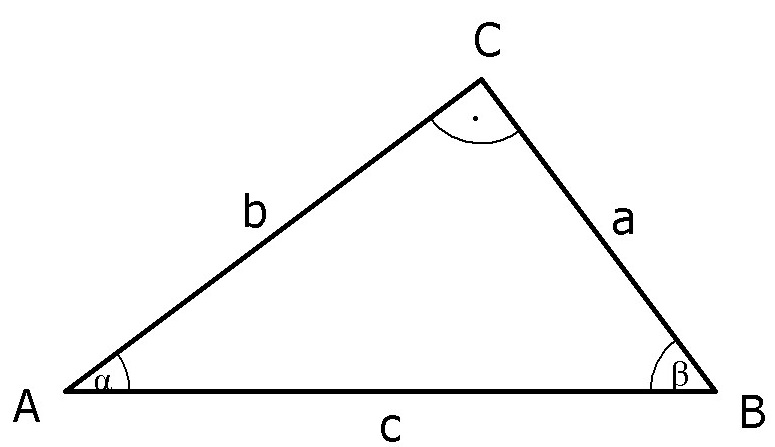
\includegraphics[width=\textwidth]{../Mathematik_1/Bilder/trigonometrie_rechtwinkliges_dreieck_bezeichnungen.png}
\end{minipage}
	\begin{minipage}{0.6\textwidth}

		Die Hypotenuse $c$ ist die Seite im Dreieck, die  dem rechten Winkel gegen�ber liegt. 
Die Bezeichnungen Gegenkathete und Ankathete beziehen sich jeweils auf einen der anderen Winkel. Bezogen auf den Winkel \(\alpha\) ist \(a\) die
Gegenkathete und \(b\) die Ankathete.
\end{minipage}
\end{exabox}

Der \textbf{Satz des Pythagoras} setzt die Seitenl�ngen im rechtwinkligen Dreieck in Beziehung zueinander. Er lautet:
\begin{theorembox}{Satz des Pythagoras}{ }
  Das Quadrat der Hypotenuse ist die Summe aus den Quadraten der Katheten, also $$c^2 = a^2 + b^2\,.$$
\end{theorembox}

Rechtwinklige Dreiecke mit demselben Winkel \(\alpha\) sind �hnlich.  Ihre absoluten Seitenl�ngen k�nnen daher unterschiedlich sein, die Verh�ltnisse entsprechender Seiten sind jedoch gleich.

Diese vom betrachteten Winkel abh�ngigen Seitenverh�ltnisse werden durch \textbf{Sinus} (\emph{sine}) und \textbf{Kosinus} (\emph{cosine}) beschrieben:

\begin{theorembox}{Geometrische Bedeutung von $\sin$ und $\cos$}{ }
  \begin{eqnarray*}
	  \sin(\alpha) &=& \frac{\textnormal{Gegenkathete}}{\textnormal{Hypthenuse}} = \frac{a}{c}\,,\\
    \cos(\alpha) &=& \frac{\textnormal{Ankathete}}{\textnormal{Hypotenuse}} = \frac{b}{c}\,.
  \end{eqnarray*}
\end{theorembox}

Wegen des Satzes des Pythagoras gilt:
\begin{theorembox}{Trigonometrischer Pythagoras - Kreisgleichung}{ }
	\[  (\sin(\alpha))^2 + (\cos(\alpha))^2 = \dfrac{a^2}{c^2} + \dfrac{b^2}{c^2} = \dfrac{a^2+b^2}{c^2}  = 1\,.\]
\end{theorembox}

Das Verh�ltnis der Katheten zueinander hei�t \textbf{Tangens} (\emph{tangent}) bzw. \textbf{Kotangens} (\emph{cotangent}). Das kann man auch mit Sinus und Kosinus ausdr�cken:
\begin{theorembox}{geometrische Bedeutung von $\tan$ und $\cot$}{ }
  \begin{eqnarray*}
    \tan(\alpha) &=&  \frac{\textnormal{Gegenkathete}}{\textnormal{Ankathete}} = \frac{a}{b}\,,\\
    \cot(\alpha) &=&  \frac{\textnormal{Ankathete}}{\textnormal{Gegenkathete}}  = \frac{b}{a}\,.
  \end{eqnarray*}
\end{theorembox}

F�r die Winkel $0^\circ$, $30^\circ$, $45^\circ$, $60^\circ$, $90^\circ$ lassen sich Sinus, Kosinus, Tangens und Kotangents gemetrisch bestimmen:
\begin{center}
  \begin{tabular}{c | c | c | c | c}
    $\alpha$ & $\sin(\alpha)$ & $\cos(\alpha)$ & $\tan(\alpha) $ & $\cot(\alpha)$ \\
    \hline
    $0^\circ$ & $0$ & $1$ & $0$ & -- \\ 
    $30^\circ$ & $1/2$ & $\sqrt{3}/2$ & $1/\sqrt{3}$ & $\sqrt{3}$ \\ 
    $45^\circ$ & $1/\sqrt{2}$ & $1/\sqrt{2}$ & $1$ & $1$ \\ 
    $60^\circ$ & $\sqrt{3}/2$ & $1/2$ & $\sqrt{3}$ & $1/\sqrt{3}$ \\ 
    $90^\circ$ & $1$ & $0$ & -- & $0$ 
  \end{tabular}
\end{center}

\subsection{Allgemeine Dreiecke (+)}

Betrachtet man allgemeine, ebene Dreiecke, so lassen gilt der \textbf{Sinussatz}: die H�he in einem allgemeinen, ebenen Dreieck l��t sich auf zwei Arten berechnen:
$$
    h = b \cdot \sin(\alpha) = a \cdot \sin(\beta) \quad \Rightarrow \frac{\sin(\alpha)}{a} =  \frac{\sin(\beta)}{b}\,.
$$

Weil im allgemeinen Dreieck keine der drei Seiten eine Sonderrolle hat, muss insgesamt gelten:
\begin{theorembox}{Sinussatz}{ }
  $
  \displaystyle{\frac{\sin(\alpha)}{a}} =  \displaystyle{\frac{\sin(\beta)}{b}} = \displaystyle{\frac{\sin(\gamma)}{c}} \quad 
  \Leftrightarrow \displaystyle{\frac{a}{\sin(\alpha)}} = \displaystyle{\frac{b}{\sin(\beta)}} = \displaystyle{\frac{c}{\sin(\gamma)}}\,.
  $
\end{theorembox}
Der Sinussatz dient dazu eine unbekannte Gr��e eines allgemeinen Dreiecks zu bestimmen.

Eine Verallgemeinerung des Satzes von Pythagoras auf allgemeine, ebene Dreiecke ist der \textbf{Kosinussatz}. Er beschreibt, wie die Quadrate der Seiten eines allgemeinen Dreiecks zueinander in Beziehung stehen. 
\vspace{0.2cm}

	\begin{minipage}{0.4\textwidth}
	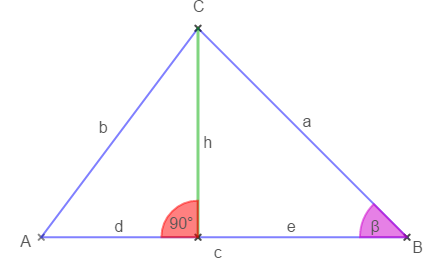
\includegraphics[width=\textwidth]{../Mathematik_1/Bilder/trigonometrie_kosinussatz_hoehenzerlegung.png}
\end{minipage}
	\begin{minipage}{0.6\textwidth}
	$$\begin{array}{rcl} b^2 &=& h^2+d^2 = \left(a\cdot \sin(\beta)\right)^2 + \left( c-a\cdot \cos(\beta)\right)^2 \\
		&=& c^2 - 2\cdot a \cdot c\cos(\beta) + a^2 \underbrace{\left( (\sin(\beta))^2 + (\cos(\beta))^2 \right)}_{\displaystyle{=1}} \\
		&&\Rightarrow b^2 = c^2 - 2\cdot a \cdot c\cos(\beta) + a^2
	\end{array} $$
\end{minipage}
\vspace{0.2cm}

Das muss f�r alle Seiten gleicherma�en gelten. Der Kosinussatz verallgemeinert den Satz des Pythagoras auf allgemeine Dreiecke. In diesen Situationen kann man damit eine unbekannte Gr��e eines allgemeinen Dreiecks bestimmen:
\begin{theorembox}{Kosinussatz}{ }
  \begin{eqnarray*}
    b^2 &=& a^2 + c^2 - 2\cdot a\cdot c \cos\beta\,, \\
    a^2 &=& b^2 + c^2 - 2\cdot b\cdot c \cos\alpha\,, \\
    c^2 &=& a^2 + b^2 - 2\cdot a\cdot b \cos\gamma\,.
  \end{eqnarray*}
\end{theorembox}

\subsection{Was ist das Bogenma�?}

%Dass eine volle Umdrehung als $360^\circ$ bezeichnet wird, ist ein Erbst�ck von den Babyloniern mit ihrem $60$er-Zahlensystem (Einstellung $\mathrm{Deg}$ auf dem Taschenrechner). Man k�nnte zum Beispiel auch $400\mathrm{gon}$ f�r eine Umdrehung nehmen, so dass ein rechter Winkel $100\mathrm{gon}$ oder Neugrad hat (Einstellung $\mathrm{Grad}$ auf dem Taschenrechner). 

Die  nat�rliche  Art,  Winkel  anzugeben,  ist das \textbf{Bogenma�} (\emph{radian}) (Einstellung $\mathrm{Rad}$ auf dem Taschenrechner). Das Bogenma� gibt an, welchen Bogen der Winkel aus dem Einheitskreis abschneidet:\marginpar{\small Aufgaben}
\begin{exabox}{Bogenma�}{ }
	\begin{minipage}{0.4\textwidth}
	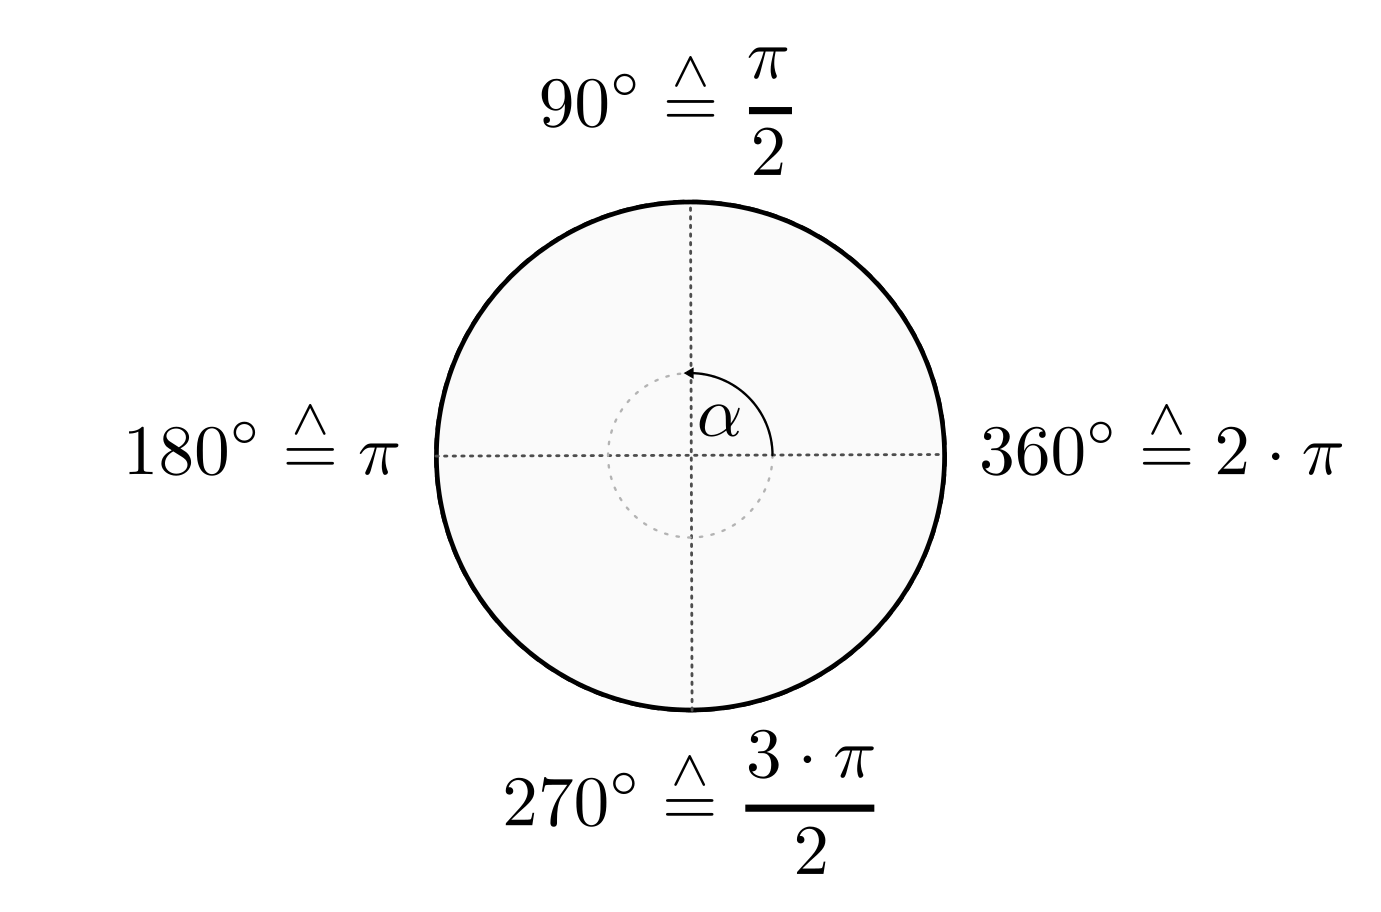
\includegraphics[width=\textwidth]{../Mathematik_1/Bilder/trigonometrie_gradmass_bogenmass.png}
  \end{minipage}
	\begin{minipage}{0.6\textwidth}
    \begin{tabular}{c c c}
    Gradma� & Bogenma� \\
    \hline
    $360^\circ$ & $\widehat = $ & $2\pi $ \\
    $180^\circ$ & $\widehat = $ & $\pi  $ \\
    $90^\circ $ & $\widehat = $ & $\pi/2$ \\
    $60^\circ $ & $\widehat = $ & $\pi/3$ \\
    $45^\circ $ & $\widehat = $ & $\pi/4$
  \end{tabular}
\end{minipage}
\end{exabox}
\noindent\textbf{Bemerkungen:}
\begin{itemize}
	\item Mit Hilfe des Dreisatzes kann man leicht jeden Winkel in Bogenma� umrechnen. Es gilt 
		\[ \varphi_{\mathrm{rad}} = \varphi_{\mathrm{deg}} \cdot \dfrac{\pi}{180^\circ} \] und umgekehrt 
		\[ \varphi_{\mathrm{deg}} = \varphi_{\mathrm{rad}} \cdot \dfrac{180^\circ}{\pi}. \] 

\item Bis auf wenige Ausnahmen %(zum Beispiel einige Teile der 3D-Programmierschnittstelle  OpenGL)  
gibt  man  beim  Programmieren  und  in mathematischer Software Winkel im Bogenma� an. Viele Formeln vereinfachen sich drastisch im Bogenma� und insbesondere gilt $\sin'=\cos$ nur im Bogenma�.
%\begin{center}
%	\includegraphics[width=0.8\textwidth]{../Mathematik_1/Bilder/14_Ableitung_sinus.png}
%\end{center}
\end{itemize}

\subsection{Trigonometrische Funktionen}

Die Definition mithilfe rechtwinkliger Dreiecke beschreibt Sinus und Kosinus zun�chst nur f�r Winkel zwischen \(0\) und \(\pi/2\). Mithilfe des Einheitskreises lassen sich beide Funktionen auf beliebige reelle Winkel erweitern.

Zu einem Winkel \(\varphi\in\mathbb R\) geh�rt auf dem Einheitskreis der Punkt
\[
P(\varphi)
=
\bigl(\cos(\varphi),\sin(\varphi)\bigr).
\]
Der Kosinus ist damit die \(x\)-Koordinate und der Sinus die \(y\)-Koordinate des zugeh�rigen Punktes auf dem Einheitskreis.

\begin{defbox}{Winkelfunktionen f�r \(\varphi \in \mathbb R\)}{ }
	\centering
	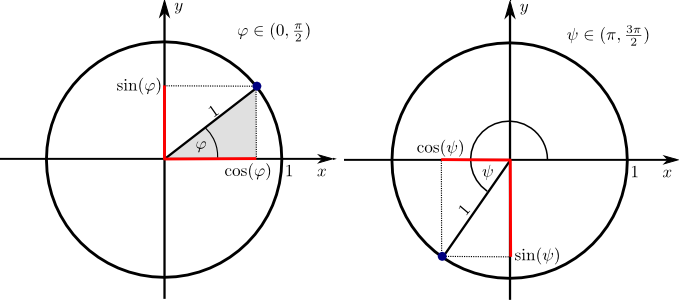
\includegraphics[width=0.6\textwidth]{../Mathematik_1/Bilder/trigonometrie_einheitskreis_sinus_kosinus.png}
\end{defbox}
Und so werden trigonometrische Funktionen zu periodischen Funktionen:
\begin{defbox}{Periodische Funktion}{ }
	\centering
	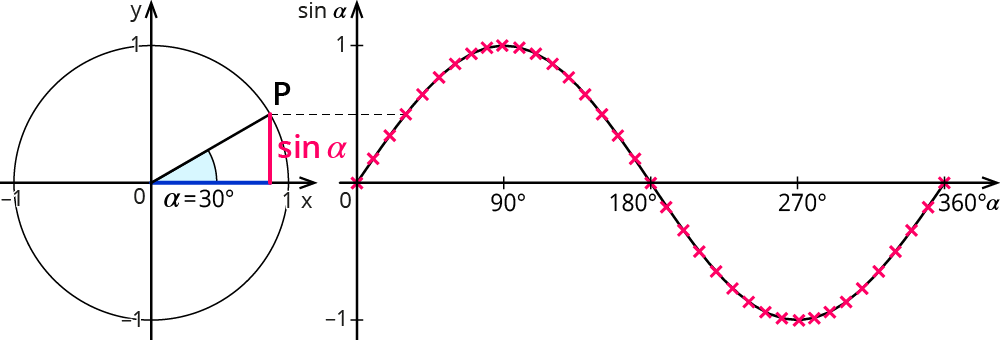
\includegraphics[width=0.6\textwidth]{../Mathematik_1/Bilder/trigonometrie_einheitskreis_sinusverlauf.png}
\end{defbox}

In der folgenden Box sind Eigenschaften der trigonometrischen Funktionen zusammengefasst:

\begin{theorembox}{Eigenschaften trigonometrischer Funktionen}{ }
	F�r alle $k\in \mathbb Z$ gilt:
	\begin{center}
		\begin{tabular}{l | l | l | l | l | l | l}
			 & Definitionsbereich & Bildmenge & Symmetrie & Periode & Nullstellen & Pole \\
			\hline
			$\sin$ & $\mathbb R$ & $[-1,1]$ & ungerade & $2\pi$ & $k\cdot \pi$ & -- \\
			$\cos$ & $\mathbb R$ & $[-1,1]$ & gerade & $2\pi$ & $\pi/2 + k\cdot \pi$ & -- \\
			$\tan$ & $\mathbb R\setminus \{ \pi/2+k\cdot \pi\}$ & $\mathbb R$ & ungerade & $\pi$ & $k\cdot \pi$ & $\pi/2+k\cdot \pi$ \\
			$\mathrm{cot}$ & $\mathbb R\setminus \{ k\cdot \pi\}$ & $\mathbb R$ & ungerade & $\pi$ & $\pi/2+k\cdot \pi$ & $k\cdot \pi$ 
		\end{tabular}
	\end{center}
\end{theorembox}

% Den Sinus und den Kosinus braucht man in den Naturwissenschaften zur Beschreibung von harmonischen Schwingungen und deren �berlagerungen. Eine Schwingung ist eine sich zeitlich wiederholende Ver�nderung einer Zustandsgr��e. 
% \begin{defbox}{Harmonische Schwingung}{ }
% 	Eine harmonische Schwingung wird durch 
% 	$$ s(t) = A\cdot \sin(\omega\cdot t + \varphi_0)\quad \textnormal{bzw.}\quad c(t) = A\cdot \cos(\omega\cdot t+ \varphi_0) $$
% 	beschrieben, wobei
% 	\begin{itemize}
% 		\item \(A\) die Amplitude,
% 		\item $\varphi_0$ die Nullphase und 
% 		\item \(\omega\) die Kreisfrequenz der Schwingung ist.
% 	\end{itemize}
% 	Das zeitabh�ngige Argument einer harmonischen Schwingung, $\varphi(t) = \omega\cdot t + \varphi_0$, bezeichnet man als Phase. 
% 	Die Schwingungsdauer oder Periode $T$ und die Frequenz $f$ betragen $$ T = \frac{2\pi}{\omega}, \quad f= \frac{1}{T} = \frac{\omega}{2\pi}\,. $$
% \end{defbox}

\subsection{Arkusfunktionen}\label{MA1-trigonometrische-funktionen-arkusfunktionen}

Um von Seitenverh�ltnissen oder mit dem Sinus- oder dem Kosinussatz auf Winkel zu schlie�en, muss man die Winkelfunktion umkehren. Allerdings sind trigonometrische Funktionen periodisch, also \underline{nicht umkehrbar}\randverweis{MA1-eigenschaften-von-funktionen}. Die Idee besteht darin, einen sinnvollen Winkel zur�ckzuliefern -- auch wenn das nicht der einzig m�gliche ist. Und genau das machen die Arkusfunktionen\footnote{Arkus $=$ Bogen, also Winkel}.

\begin{defbox}{Arkusfunktionen}{ }
	\begin{eqnarray*}
		\begin{array}{lcl l }
			\arcsin: [-1,1] &\to& [-\pi/2, \pi/2], \; &x\mapsto \arcsin(x) \\[1ex]
			\arccos: [-1,1] &\to& [0, \pi], \; &x\mapsto \arccos(x)  \\[1ex]
			\arctan: (-\infty,\infty) &\to& (- \pi/2, \pi/2), \; &x\mapsto \arctan(x)\\[1ex]
			\mathrm{arccot}: (-\infty,\infty) &\to& (0,\pi), \; &x\mapsto \mathrm{arccot}(x) 
\end{array}
\end{eqnarray*}
\textbf{Bemerkung:} es gilt $\mathrm{arccot}(x) = \frac{\pi}{2} - \arctan(x)$.
\end{defbox}

\noindent \textbf{Bemerkungen:}
\begin{itemize}
	\item �hnlich wie bei geradzahligen \underline{Potenzfunktionen}\randverweis{MA1-potenz-und-wurzelfunktionen} ist die Idee eine trigonometrische Funktion auf ein maximales Intervall einzuschr�nken, auf dem sie injektiv ist. Das Intervall ist zun�chst willk�rlich.
	Der Sinus ist auf dem Intervall
\[
I=[-\pi/2,\pi/2]
\]
streng monoton steigend und damit injektiv. Gleichzeitig nimmt er dort alle
Werte aus \([-1,1]\) an. Die Einschr�nkung
\[
\sin:[-\pi/2,\pi/2]\to[-1,1]
\]
ist daher bijektiv und besitzt eine Umkehrfunktion. Die Umkehrfunktion, die den Sinus auf \(I\) umkehrt, nennt sich \textbf{Arkussinus}.  

	\item Dass die  Arkussinus Funktion  keine  Winkel  �ber  $90^\circ$ liefert, ist  dann  gef�hrlich, wenn man mit dem Sinussatz arbeitet: Bei der Anwendung des Sinussatzes kann aus
\[
\sin(\beta)=s
\]
nicht unmittelbar auf einen eindeutigen Winkel geschlossen werden. F�r
\(0<s<1\) besitzen im Intervall \((0,\pi)\) im Allgemeinen die beiden Winkel
\[
\beta
\qquad\text{und}\qquad
\pi-\beta
\]
denselben Sinuswert. Je nach den �brigen gegebenen Gr��en k�nnen daher zwei verschiedene Dreiecke m�glich sein.	
	\item Der Arkustangens liefert also nur Werte von $-90^\circ \widehat= -\pi/2$ bis $90^\circ \widehat =\pi/2$ und keine gesamte Umdrehung von $-180^\circ=-\pi$ bis $180^\circ =\pi$. Das Problem ist, dass der Tangens nicht unterscheiden kann, ob ein Punkt \( (x|y)\) im ersten oder dritten bzw. im zweiten oder vierten Quadranten liegt, denn die Vorzeicheninformation geht bei der Division verloren:
$$\tan(\varphi) = \frac{y_1}{x_1} =\frac{y_2}{x_2} = \tan(\varphi +\pi), \quad \mathrm{mit} \; y_2=-y_1, \quad x_2=-x_1\,.$$ 
\end{itemize}

Das zuletzt genannte Problem kann behoben werden, wenn man die Vorzeicheninformation der Koordinaten \(x\) und \(y\) wei� und genau das wird in der Praxis auch getan: in fast allen Programmiersprachen gibt es eine Funktion namens $\verb-atan2-$. Diese Funktion liefert Werte aus $(-\pi,\pi]$ zur�ck, also eine komplette Umdrehung. Die getrennte �bergabe der Koordinaten \(x\) und \(y\) erh�lt die Vorzeicheninformation: \footnote{Normalerweise ist die Reihenfolge $y$ dann $x$,  entsprechend $"\dfrac{y}{x}"$, aber man muss aufpassen, denn manchmal ist die Reihenfolge auch "$x,y$".}

\begin{exabox}{\(\mathrm{atan2}\)}{ }
	\begin{minipage}{0.4\textwidth}
	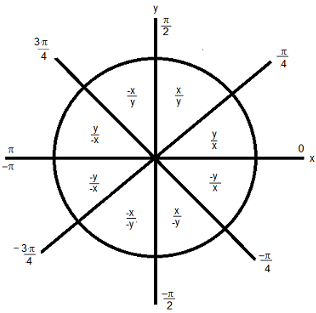
\includegraphics[width=\textwidth]{../Mathematik_1/Bilder/trigonometrie_atan2_quadranten_winkel.png}
\end{minipage}
	\begin{minipage}{0.6\textwidth}
		Der herk�mmliche Arkustangens kann Punkte im ersten und dritten Quadranten nicht unterscheiden: 
		\[ 
			\begin{array}{rcl} 
				(3|3) &\Rightarrow & \begin{cases} \verb-atan2-(3,3) &= \frac14 \pi \,,\\ \arctan(1) &= \frac14 \pi \end{cases}\\[2ex] 
				(-3|-3) &\Rightarrow & \begin{cases} \verb-atan2-(-3,-3) &= -\frac34 \pi \,,\\ \arctan(1) &= \frac14 \pi \end{cases}\\[2ex] 
			\end{array}
		\]
		Der herk�mmliche Arkustangens kann Punkte im zweiten und vierten Quadranten nicht unterscheiden: 
		\[ 
			\begin{array}{rcl} 
				(-3|3) &\Rightarrow & \begin{cases} \verb-atan2-(3,-3) &= \frac34 \pi \,,\\ \arctan(-1) &= -\frac{1}{4} \pi \end{cases}\\[2ex] 
				(3|-3) &\Rightarrow & \begin{cases} \verb-atan2-(-3,3) &= -\frac14 \pi \,,\\ \arctan(-1) &= -\frac14 \pi \end{cases}
			\end{array}
		\]
	\end{minipage}
\end{exabox}

Der Arkustangens kommt dann zum Einsatz, wenn man von kartesischen Koordinaten in Polarkoordinaten umrechnen m�chte. 
\begin{defbox}{Polarkoordinaten mit Hilfe von \(\mathrm{atan2}\) }{ }
	Jeder Punkt $(x,y) \in \mathbb R^2$ kann in der Form 
	$$ 
	x= r\cdot \cos(\varphi), \quad y=r\cdot \sin(\varphi)
	$$ 
	mit $r\in \mathbb R^+_0$ und $\varphi \in (-\pi, \pi]$ dargestellt werden. Es gilt 
	$$
	r=\sqrt{x^2+y^2}, \quad 
\varphi=\operatorname{atan2}(y,x):=
\begin{cases}
\arctan(y/x), & x>0,\\[1ex]
\arctan(y/x)+\pi, & x<0,\;y\geq0,\\[1ex]
\arctan(y/x)-\pi, & x<0,\;y<0,\\[1ex]
\pi/2, & x=0,\;y>0,\\[1ex]
-\pi/2, & x=0,\;y<0.
\end{cases}
	$$
	\noindent{\textbf{Bemerkungen}}
	\begin{itemize}
		\item Die Werte $(r,\varphi)$ hei�en Polarkoordinaten von $(x,y)$.
		\item F�r den Ursprung \( (0,0)\) ist der Winkel \(\varphi \) nicht definiert.
		\item Die Funktion \(\operatorname{atan2}\) besitzt damit die folgende Signatur: \[ \operatorname{atan2}: \mathbb R^2 \setminus \{ (0, 0 )\} \to (-\pi, \pi]\].
	\end{itemize}
\end{defbox}


\begin{exabox}{L�sen einer trigonometrischen Gleichung}{ }

	Gesucht sind \emph{alle} reellen L�sungen der Gleichung
\[
\sin(x)=\frac12.
\]

Aus den bekannten Werten der Sinusfunktion folgt zun�chst
\[
\sin\left(\frac{\pi}{6}\right)=\frac12.
\]
Damit ist
\[
x_1=\frac{\pi}{6}
\]
\emph{eine} L�sung der Gleichung.

Diese L�sung ist jedoch nicht die einzige. Am Einheitskreis entspricht der Sinus der \(y\)-Koordinate eines Punktes. Die \(y\)-Koordinate \(\frac12\) wird innerhalb einer vollst�ndigen Periode an zwei verschiedenen Stellen angenommen. Aufgrund der Symmetrie des Sinus gilt
\[
\sin(x)=\sin(\pi-x).
\]
Aus
\[
x_1=\frac{\pi}{6}
\]
ergibt sich daher als zweite L�sung innerhalb des Intervalls
\([0,2\pi)\)
\[
x_2
=
\pi-\frac{\pi}{6}
=
\frac{5\pi}{6}.
\]

Damit besitzt die Gleichung innerhalb einer vollst�ndigen Periode zwei L�sungen, \( x_1 = \frac{\pi}{6}\) und \(x_2 = \frac{5\pi}{6}\).

Da die Sinusfunktion die Periode \(2\pi\) besitzt, wiederholen sich diese
L�sungen nach jeder vollst�ndigen Umdrehung:
\[
\sin(x+2k\pi)=\sin(x),
\qquad k\in\mathbb Z.
\]
Damit ergeben sich alle reellen L�sungen zu
\[
x=\frac{\pi}{6}+2k\pi
\quad\text{oder}\quad
x=\frac{5\pi}{6}+2k\pi,
\qquad k\in\mathbb Z.
\]

Die L�sungsmenge kann entsprechend geschrieben werden als
\[
\mathbb L
=
\left\{
\frac{\pi}{6}+2k\pi:k\in\mathbb Z
\right\}
\cup
\left\{
\frac{5\pi}{6}+2k\pi:k\in\mathbb Z
\right\}.
\]

Das Beispiel zeigt einen wesentlichen Unterschied zu vielen bisher
betrachteten Gleichungen: Aufgrund der Periodizit�t einer trigonometrischen
Funktion k�nnen aus einer L�sung unendlich viele weitere L�sungen entstehen.
F�r die vollst�ndige L�sungsmenge m�ssen daher sowohl die verschiedenen
L�sungen innerhalb einer Periode als auch die periodischen Wiederholungen
ber�cksichtigt werden.

\end{exabox}
 \newpage % Trigonometrische Funktionen
\setcounter{exercise}{0} 
\ifintegriereaufgaben
\section*{Trigonometrische Funktionen Aufgaben}\label{MA1-trigonometrische-funktionen-aufgaben}

	Regeln und Beispiele, die zur Bearbeitung der Aufgaben hilfreich sind, finden Sie im Skript\wennreferenzvorhanden{MA1-trigonometrische-funktionen}{ (Abschnitt \abschnittsverweis{MA1-trigonometrische-funktionen})} und, falls Sie nicht weiterkommen, schauen Sie \hyperref[MA1-trigonometrische-funktionen-loesungen]{hier}.
\else 
\section{Trigonometrische Funktionen Aufgaben}\label{MA1-trigonometrische-funktionen-aufgaben}

	Regeln und Beispiele, die zur Bearbeitung der Aufgaben hilfreich sind, finden Sie im Skript und, falls Sie nicht weiterkommen, schauen Sie \hyperref[MA1-trigonometrische-funktionen-loesungen]{hier}.
\fi 

\begin{exercisebox}[Harmonische Schwingungen] %Andreas
	Bestimmen Sie die Amplitude, die Periode und die Nullphase der folgenden harmonischen Schwingungen und skizzieren Sie den Funktionsverlauf.
	\begin{eqnarray*}
		(a)\; t\mapsto 2\cdot \sin\left(3t-\frac{\pi}{6}\right) \quad \quad \quad \quad  (b)\; t\mapsto 10\cdot \sin(\pi t - 3)
	\end{eqnarray*}
\end{exercisebox}

\begin{exercisebox}[Interpolation] %Andreas
	Eine Funktion der Form \[ f: x\mapsto \frac{a_0}{2} + a_1 \cos(x) + b_1\sin(x)\] soll durch die Punkte $(x_i, y_i),\, i=1,2,3$ mit \[ (0|1), (\pi/6|-1), (\pi/2|-3)\]
	gelegt werden. Bestimmen Sie ein Gleichungssystem f�r die Koeffizienten $a_0, a_1, b_1$ und l�sen Sie es.
\end{exercisebox}

\begin{exercisebox}[Gleichungen] %Andreas
	Bestimmen Sie alle L�sungen der folgenden Gleichungen:
	\begin{eqnarray*}
		\begin{array}{ll}
			(a) \; \sin(2x+5) = 0,4 \quad \quad \quad & (b) \;\tan\left( 2(x+1)\right) = 1 \\[1ex] (c)\; \sqrt{\cos(x-1)} = 2^{-1/4} \quad \quad \quad & (d) \; \sin(x) = \sqrt{1-\sin^2(x)} 
		\end{array}
	\end{eqnarray*}
\end{exercisebox}

\begin{exercisebox}[Kreisgleichung] %Lucy
	Bestimmen Sie die Schnittpunkte der angegebenen Geraden $g$ mit dem Kreis $k:=\{(x,y):\; x^2+y^2=4\}$:
	\begin{eqnarray*}
		\begin{array}{lll}
		(a)\; g_1: x\mapsto x-2 \quad\quad (b) \; g_2: x\mapsto x-4 \quad\quad (c)\; g_3: x\mapsto 2 \end{array}
	\end{eqnarray*}
\end{exercisebox}

\begin{exercisebox}[Kreisgleichung] %Lucy
	Welche der Gleichungen beschreiben einen Kreis? Bestimmen Sie gegebenenfalls die Mittelpunkte und die Radien.
			\begin{eqnarray*} 
				\begin{array}{lll} 
					(a) \; (x+2)^2 + y^2 = 64 \quad \quad & (b)\; (x-5)^2 + (y+2)^2 = 0 \quad \quad & (c) \; x^2 + y^2 - 2x + 4y -20 = 0 \\[1ex] (d) \;x^2 + y^2 - 2x + 2y + 14 = 0 \quad \quad & (e) \; x^2 + y^2 +y = 0 &
				\end{array}
			\end{eqnarray*}
\end{exercisebox}

\begin{exercisebox}[Qualitativer Graph] %Lovis
	\begin{itemize}
		\item[(a)] Zeichnen Sie die Funktion $f: x\mapsto 2\cdot \sin(x-\frac{\pi}{2})-2$ auf dem Intervall  $[-\pi,3\pi]$ und lesen Sie aus dem Graphen den Bildbereich, die Nullstellen und die Extremstellen von $f$ ab.
		\item[(b)] Zeichnen Sie die Funktion $f: x\mapsto -\sin(x-\pi)$ auf dem Intervall  $[0,\frac{5\pi}{2}]$ und lesen Sie aus dem Graphen den Bildbereich, die Nullstellen und die Extremstellen von $f$ ab.
	\end{itemize}
\end{exercisebox}

%\begin{exercisebox}[Newton-Verfahren, $\pi$]
%Bestimme $\pi$ mit Hilfe des Newton-Verfahrens auf vier Dezimalstellen genau.
%\end{exercisebox}

%\begin{exercisebox}[Titanic]
%	Gro�kreise, Dreiecke auf gekr�mmten Mannigfaltigkeiten
%\end{exercisebox}
%
%\begin{exercisebox}[Schwingungen]
%	Basis, Akustik
%\end{exercisebox}


%\begin{exercisebox}[Dreiecke]
%\end{exercisebox}
 \newpage 
\setcounter{satz}{0} \setcounter{def}{0} \setcounter{exa}{0}  \section{Verkettung von Funktionen}\label{MA1-verkettung-von-funktionen}

\begin{table}[H]
  \centering
  \begin{tabularx}{\textwidth}{p{0.9\textwidth} p{0.1\textwidth}}
    \toprule
	  \multicolumn{2}{c}{\textbf{�bersicht �ber Lernziele und Voraussetzungen}}\\
    \midrule
    \textbf{Lernziele} &\\[.5\normalbaselineskip]
\tabitem verkettete Funktionen erkennen und in ihre Teilfunktionen zerlegen &\\
\tabitem die Abbildungsvorschrift einer Verkettung bestimmen &\\
\tabitem Definitionsbereich und Bildmenge einer Verkettung bestimmen &\\
\tabitem Verschiebung, Skalierung und Spiegelung von Funktionsgraphen als Verkettungen darstellen &\\
\tabitem Funktionsgraphen durch Kompositionen systematisch ver�ndern &\\
\tabitem harmonische Schwingungen aus der Sinusfunktion systematisch konstruieren und die Bedeutung ihrer Parameter erkl�ren &\\[.5\normalbaselineskip]
\midrule
\textbf{Voraussetzungen} &\\[.5\normalbaselineskip]
\tabitem Funktionsbegriff, Definitionsbereich und Bildmenge & \abschnittsverweis{MA1-funktionen}\\
\tabitem Eigenschaften von Funktionen & \abschnittsverweis{MA1-eigenschaften-von-funktionen}\\
\tabitem grundlegende Funktionsklassen & \abschnittsverweis{MA1-lineare-funktionen}-\abschnittsverweis{MA1-trigonometrische-funktionen}\\
    \bottomrule
  \end{tabularx}
\end{table}

\ifintegriereaufgaben \noindent �bungsaufgaben zum Thema finden Sie hier: \hyperref[MA1-verkettung-von-funktionen-aufgaben]{Aufgaben}
\vspace{0.3cm}
\hrule
\fi

\subsection{Was ist eine Verkettung?}

Funktionen k�nnen nicht nur miteinander addiert oder multipliziert werden.
Der Funktionswert einer Funktion kann auch als Eingabe einer weiteren
Funktion verwendet werden.

Es seien beispielsweise zwei Funktionen \(g\) und \(f\) gegeben. Zun�chst
wird \(g\) auf \(x\) angewendet:
\[
x\mapsto g(x).
\]
Das Ergebnis \(g(x)\) wird anschlie�end als Eingabe der Funktion \(f\)
verwendet:
\[
g(x)\mapsto f(g(x)).
\]

Diese Hintereinanderausf�hrung hei�t \textbf{Verkettung} oder
\textbf{Komposition} (\emph{composition}) der Funktionen \(f\) und \(g\).
Sie wird mit
\[
f\circ g
\]
bezeichnet und ist selbst wieder eine Funktion:
\[
(f\circ g)(x)=f(g(x)).
\]

Die Schreibweise \(f\circ g\) wird dabei von rechts nach links gelesen:
Zuerst wird \(g\), anschlie�end \(f\) angewendet. Daher wird
\(f\circ g\) auch als �\(f\) nach \(g\)� bezeichnet.

\begin{exabox}{Verkettung als Maschine}{ }
	\centering
	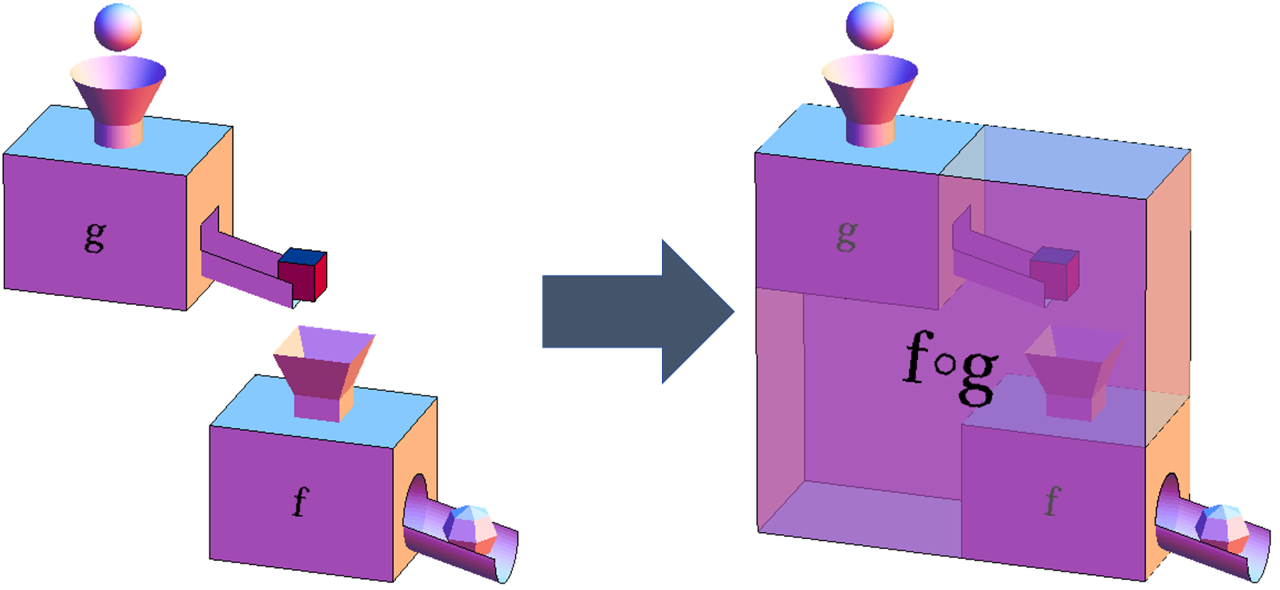
\includegraphics[width=0.7\textwidth]{../Mathematik_1/Bilder/funktionen_verkettung_maschinenmodell.png}
\end{exabox}

Die Reihenfolge ist wichtig: Verkettung ist im Allgemeinen \emph{nicht} kommutativ.

\begin{exabox}{Reihenfolge ist entscheidend}{ }

Es seien
\[
f(x)=\sin(x)
\qquad\text{und}\qquad
g(x)=e^x.
\]
Dann ergibt sich in der einen Reihenfolge
\[
(f\circ g)(x)
=
\sin(e^x),
\qquad
f\circ g:\mathbb R\to[-1,1].
\]

In der umgekehrten Reihenfolge entsteht dagegen
\[
(g\circ f)(x)
=
e^{\sin(x)},
\qquad
g\circ f:\mathbb R\to[e^{-1},e].
\]

Damit gilt im Allgemeinen
\[
f\circ g\neq g\circ f.
\]
Die Verkettung von Funktionen ist also im Allgemeinen nicht kommutativ.

\end{exabox}

Die unterschiedliche Reihenfolge ver�ndert damit nicht nur die Abbildungsvorschrift, sondern auch das Verhalten und die Bildmenge der entstehenden Funktion.

\subsubsection*{Definitionsbereich einer Verkettung}

Bei einer Verkettung muss nicht nur die innere Funktion \(g\) an der Stelle
\(x\) definiert sein. Ihr Funktionswert \(g(x)\) muss au�erdem eine zul�ssige
Eingabe f�r die �u�ere Funktion \(f\) sein.

F�r die Verkettung
\[
(f\circ g)(x)=f(g(x))
\]
gilt daher
\[
D_{f\circ g}
=
\{x\in D_g:g(x)\in D_f\}.
\]

\begin{exabox}{Definitionsbereich einer Verkettung bestimmen}{ }

Betrachtet wird die Verkettung
\[
x\mapsto\sqrt{\ln(x)}.
\]
Die innere Funktion
\[
g(x)=\ln(x)
\]
ist zun�chst nur f�r
\[
x>0
\]
definiert.

Die �u�ere Funktion
\[
f(y)=\sqrt y
\]
kann au�erdem nur nichtnegative Werte verarbeiten. Daher muss zus�tzlich
\[
\ln(x)\geq0
\]
gelten. Dies ist genau f�r
\[
x\geq1
\]
der Fall.

Damit besitzt die Verkettung den Definitionsbereich
\[
D_{f\circ g}=[1,\infty)
\]
und es gilt
\[
\sqrt{\;\cdot\;}\circ\ln:
[1,\infty)\to[0,\infty),
\qquad
x\mapsto\sqrt{\ln(x)}.
\]

\end{exabox}

\begin{exabox}{Eine verkettete Funktion in Teilfunktionen zerlegen}{ }

Betrachtet wird die Funktion
\[
x\mapsto\frac{1}{(\sin x)^2+1}.
\]

Die Abbildungsvorschrift l�sst sich als Folge von drei Schritten lesen:
\[
x
\longmapsto
\sin(x)
\longmapsto
(\sin x)^2+1
\longmapsto
\frac{1}{(\sin x)^2+1}.
\]

Dazu k�nnen die drei Funktionen
\[
h(x)=\sin(x),
\qquad
g(x)=x^2+1,
\qquad
f(x)=\frac1x
\]
definiert werden. Damit gilt
\[
(f\circ g\circ h)(x)
=
f(g(h(x)))
=
\frac{1}{(\sin x)^2+1}.
\]

Die �u�erste Rechenoperation geh�rt dabei zur �u�ersten Funktion \(f\), die
innerste Rechenoperation zur zuerst ausgef�hrten Funktion \(h\).

\end{exabox}

\noindent\textbf{Bemerkung:}
\begin{itemize}
	\item Das Erkennen solcher Verkettungen wird sp�ter bei der Differentialrechnung erneut wichtig. Die Kettenregel beschreibt, wie die Ableitung einer verketteten Funktion aus den Ableitungen ihrer Teilfunktionen bestimmt werden
kann.
\item Wird eine Funktion mehrfach mit sich selbst verkettet, spricht man von einer \textbf{Iteration}. 
F�r die dreifache Iteration findet sich daher auch die Schreibweise
\[
f^3:=f\circ f\circ f.
\]
Diese Notation ist allerdings kontextabh�ngig und darf nicht mit der dritten Potenz des Funktionswertes, also der Zahl \( (f(x))^3 \) verwechselt werden.	
\item Die Schreibweise \(f^{-1}\) bezeichnet die Umkehrfunktion von \(f\), sofern diese existiert.
\end{itemize}

\subsection{Systematische Ver�nderung von Funktionsgraphen}

Viele typische Ver�nderungen von Funktionsgraphen lassen sich als
Verkettungen mit linearen Funktionen verstehen. Dabei ist entscheidend, an
welcher Stelle der Verkettung die lineare Funktion steht.

Wird eine Funktion
\[
g(y)=my+b
\]
\textbf{nach} \(f\) angewendet, so gilt
\[
(g\circ f)(x)=m\,f(x)+b.
\]
Die Ver�nderung betrifft unmittelbar die Funktionswerte und wirkt daher in
\textbf{vertikaler Richtung}.

Wird dagegen eine lineare Funktion
\[
g(x)=k(x+a)
\]
\textbf{vor} \(f\) angewendet, so gilt
\[
(f\circ g)(x)=f\!\bigl(k(x+a)\bigr).
\]
In diesem Fall wird das Argument von \(f\) ver�ndert. Die Ver�nderung wirkt
daher in \textbf{horizontaler Richtung}.

Im Folgenden werden diese Ver�nderungen zun�chst einzeln untersucht und
anschlie�end in einem gemeinsamen Transformationsbaukasten zusammengefasst.


\subsubsection*{Ver�nderung in vertikaler Richtung}

Wird zu jedem Funktionswert \(f(x)\) eine Konstante \(b\neq0\) addiert,
ver�ndert sich nicht das Argument der Funktion, sondern ausschlie�lich ihr
Funktionswert. Der Graph wird dadurch in vertikaler Richtung verschoben:
\begin{itemize}
    \item F�r \(b>0\) erfolgt die Verschiebung um \(b\) Einheiten nach oben.
    \item F�r \(b<0\) erfolgt die Verschiebung um \(|b|\) Einheiten nach unten.
\end{itemize}

\begin{exabox}{Vertikale Translation}{ }
    \begin{minipage}{0.4\textwidth}
        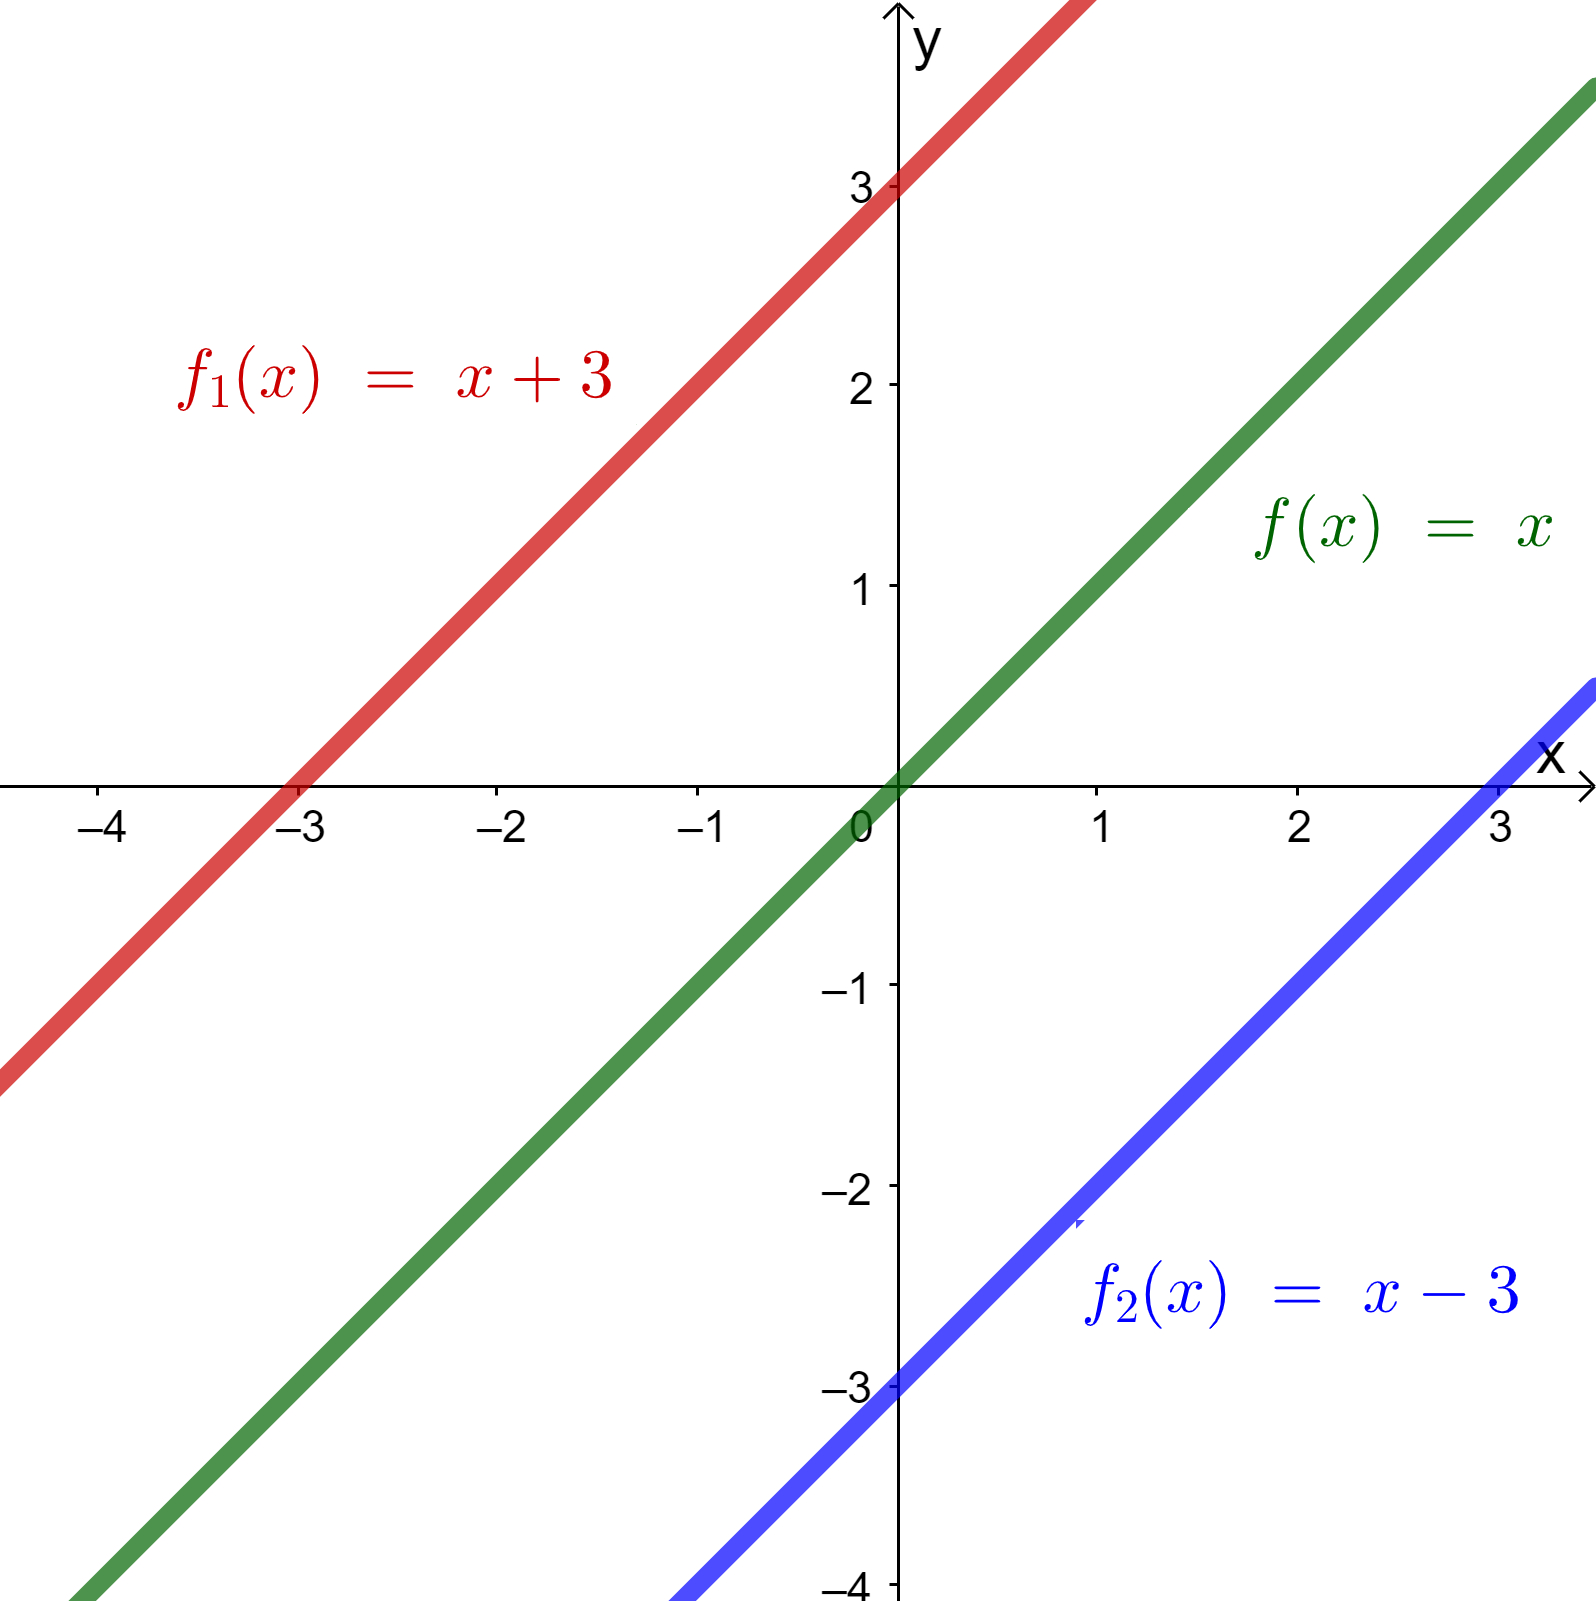
\includegraphics[width=0.95\textwidth]{../Mathematik_1/Bilder/funktionen_vertikale_verschiebung_gerade.png}
    \end{minipage}
    \begin{minipage}{0.6\textwidth}
        \begin{itemize}
            \item Originalfunktion:
            \[
            \textcolor{darkgreen}{f:x\mapsto x}
            \]

            \item Verschiebung um \(3\) Einheiten nach oben:
            \[
            \textcolor{red}{f_1:x\mapsto x+3}
            =
            \textcolor{darkgreen}{f}(x)+3
            \]

            \item Verschiebung um \(3\) Einheiten nach unten:
            \[
            \textcolor{blue}{f_2:x\mapsto x-3}
            =
            \textcolor{darkgreen}{f}(x)-3
            \]
        \end{itemize}
    \end{minipage}
\end{exabox}

Wird der Funktionswert \(f(x)\) mit einer Konstanten \(m\) multipliziert, werden seine Werte und damit ihre Abst�nde von der \(x\)-Achse mit dem Faktor \(|m|\) skaliert.
\begin{itemize}
    \item F�r \(|m|>1\) wird der Graph in vertikaler Richtung gestreckt.
    \item F�r \(0<|m|<1\) wird der Graph in vertikaler Richtung gestaucht.
    \item F�r \(m<0\) erfolgt zus�tzlich eine Spiegelung an der \(x\)-Achse.
\end{itemize}

F�r \(m=0\) werden dagegen alle Funktionswerte auf \(0\) abgebildet; es
entsteht die konstante Nullfunktion.

\begin{exabox}{Vertikale Streckung und Stauchung}{ }
    \begin{minipage}{0.5\textwidth}
        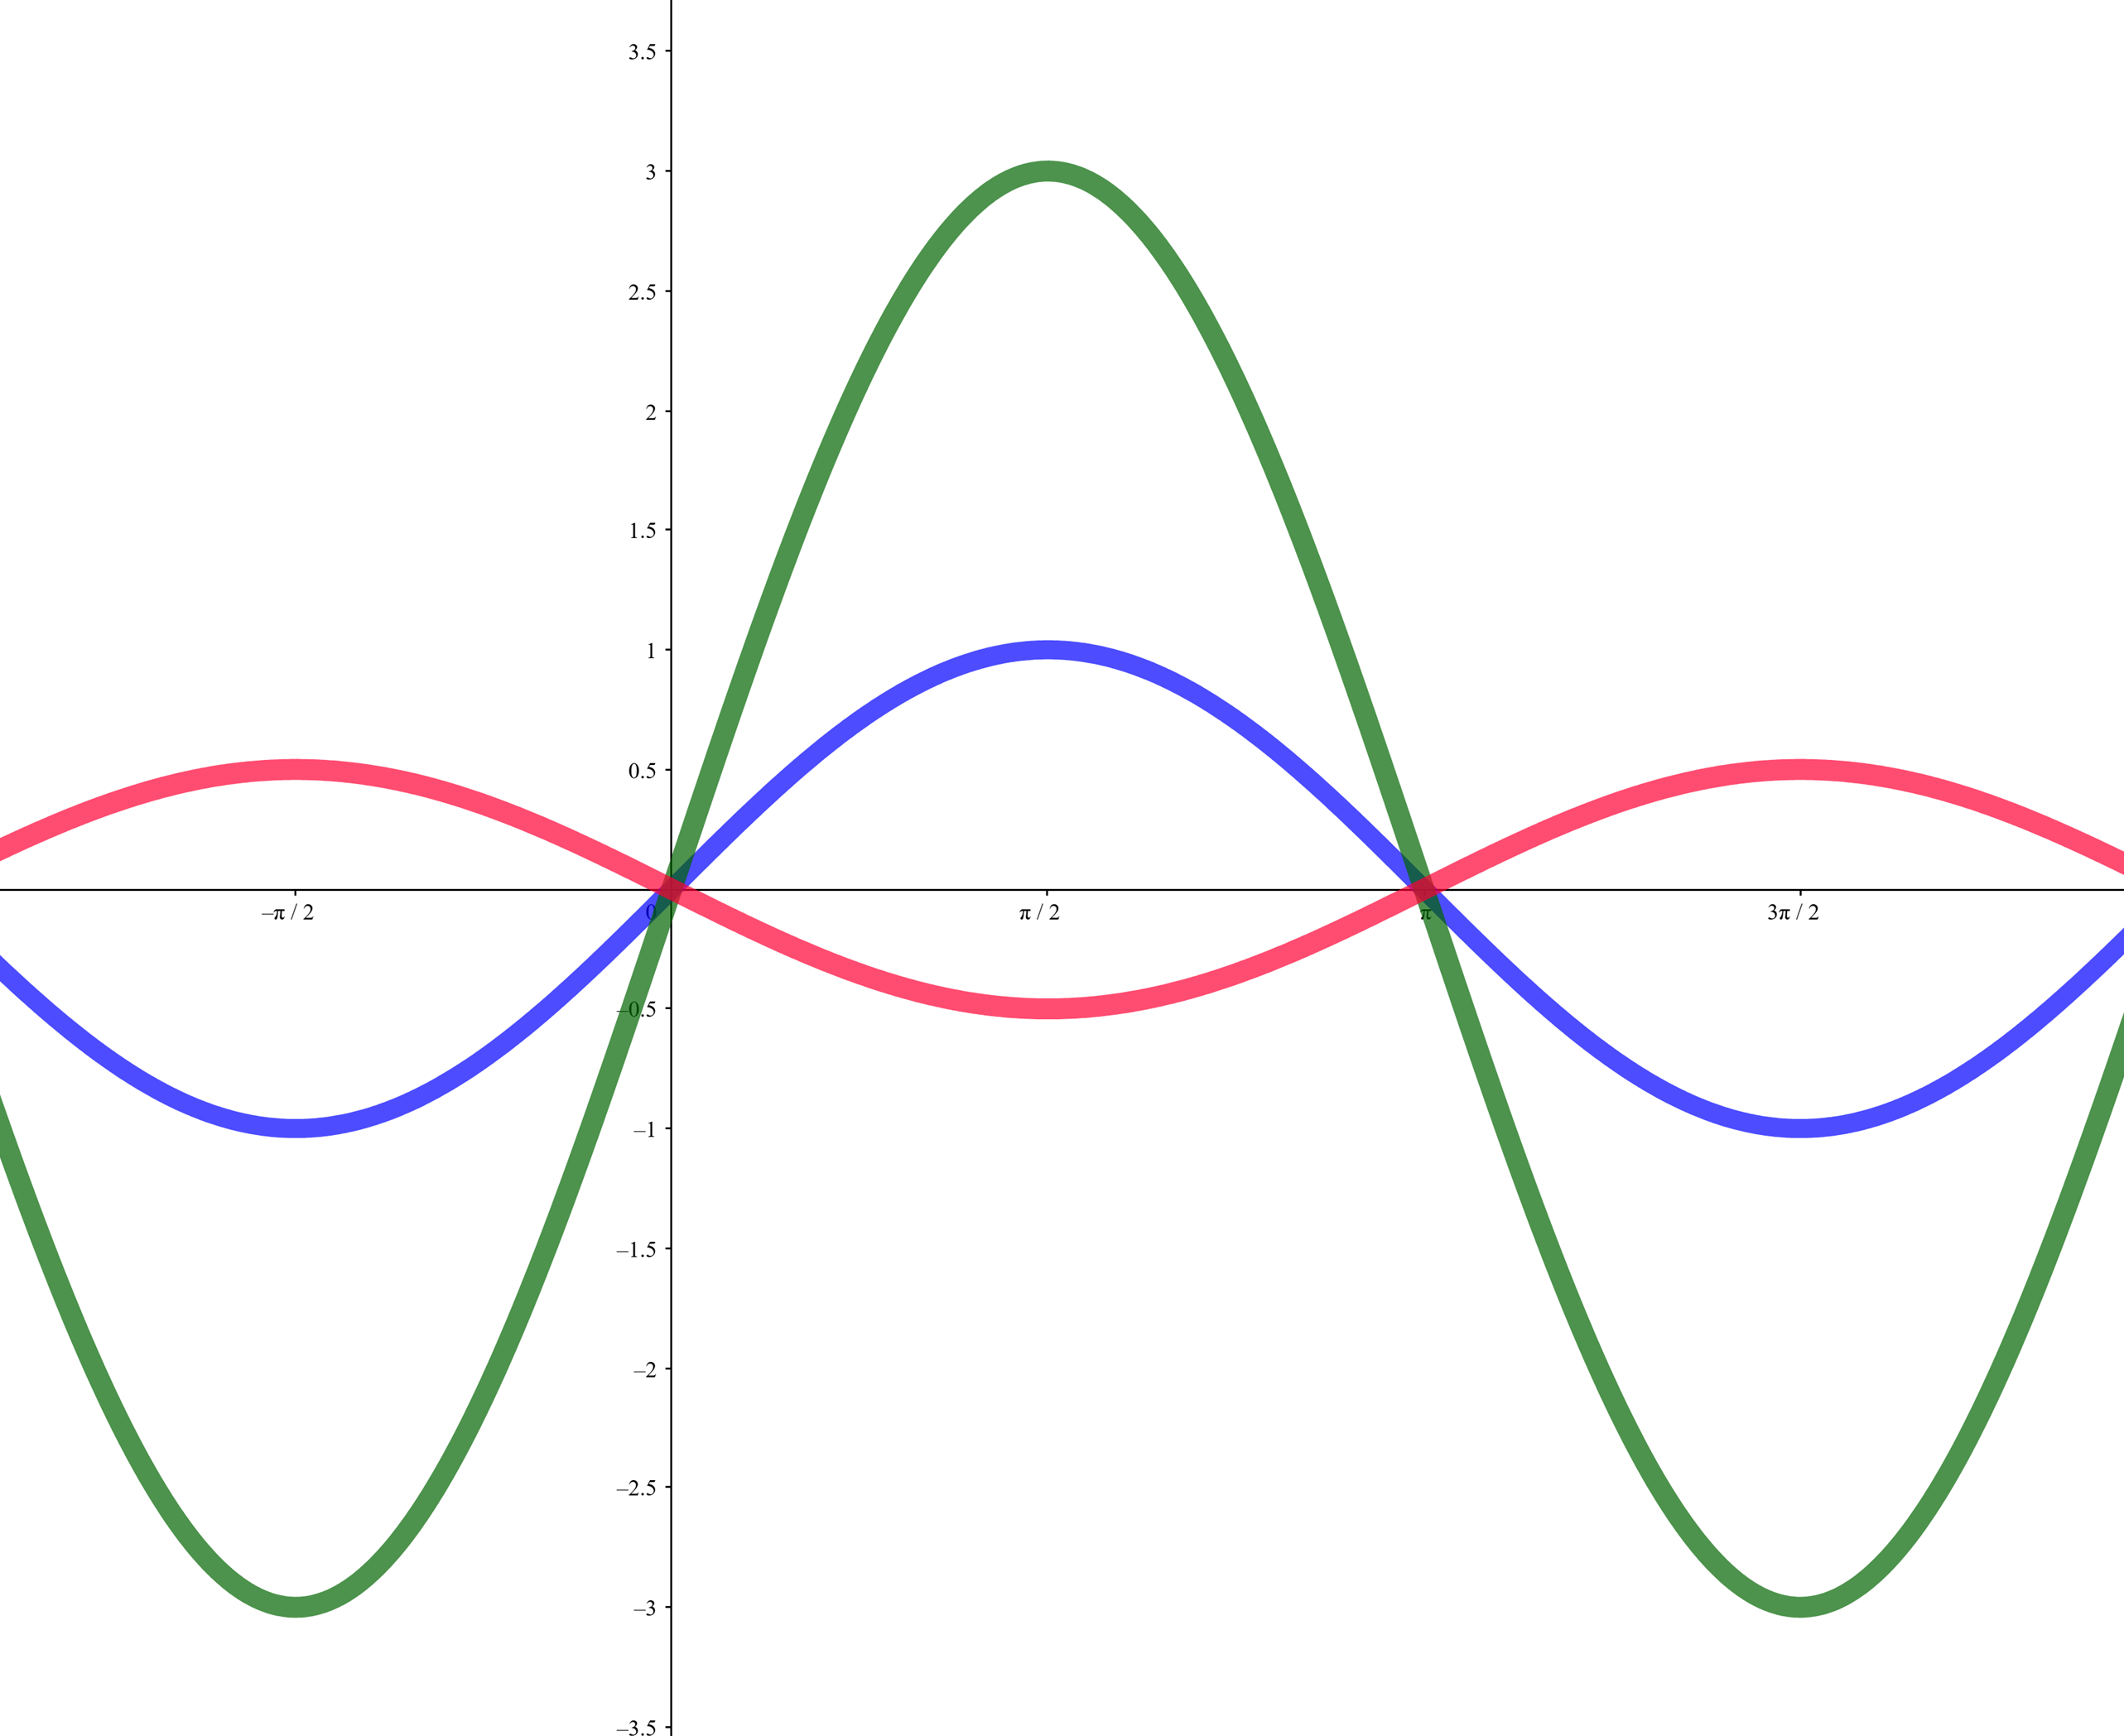
\includegraphics[width=0.95\textwidth]{../Mathematik_1/Bilder/funktionen_vertikale_skalierung_sinus.png}
    \end{minipage}
    \begin{minipage}{0.4\textwidth}
        \begin{itemize}
            \item Originalfunktion:
            \[
            \textcolor{blue}{f:x\mapsto\sin(x)}
            \]

            \item Streckung in \(y\)-Richtung:
            \[
            \textcolor{darkgreen}{f_1:x\mapsto3\sin(x)}
            =
            3\cdot\textcolor{blue}{f}(x)
            \]

            \item Stauchung in \(y\)-Richtung und Spiegelung an der
            \(x\)-Achse:
            \[
            \textcolor{red}{f_2:x\mapsto-\frac12\sin(x)}
            =
            -\frac12\cdot\textcolor{blue}{f}(x)
            \]
        \end{itemize}
    \end{minipage}
\end{exabox}

Beide vertikalen Ver�nderungen lassen sich miteinander kombinieren. F�r
\[
g(y)=my+b
\]
gilt
\[
(g\circ f)(x)=m\,f(x)+b.
\]
Dabei werden die Funktionswerte zun�chst mit \(m\) skaliert und anschlie�end
um \(b\) verschoben.


\subsubsection*{Ver�nderung in horizontaler Richtung}

Wird eine Konstante \(a\) innerhalb des Arguments von \(f\) addiert,
\[
x\mapsto f(x+a),
\]
ver�ndern sich nicht unmittelbar die Funktionswerte, sondern die Stellen,
an denen diese Funktionswerte angenommen werden. Der Graph wird dadurch in
horizontaler Richtung verschoben.

Dabei wirkt das Vorzeichen zun�chst ungewohnt. Angenommen, die urspr�ngliche
Funktion nimmt einen bestimmten Funktionswert an der Stelle \(x_0\) an. Die
ver�nderte Funktion \(f(x+a)\) nimmt denselben Funktionswert genau dann an,
wenn
\[
x+a=x_0.
\]
Daraus folgt
\[
x=x_0-a.
\]
Der urspr�ngliche Punkt wird also um \(a\) Einheiten nach links verschoben.

Damit gilt:
\begin{itemize}
    \item F�r \(a>0\) wird der Graph von \(f(x+a)\) um \(a\) Einheiten nach
          links verschoben.
    \item F�r \(a<0\) erfolgt die Verschiebung entsprechend nach rechts.
\end{itemize}

\begin{exabox}{Horizontale Translation}{ }
    \begin{minipage}{0.5\textwidth}
        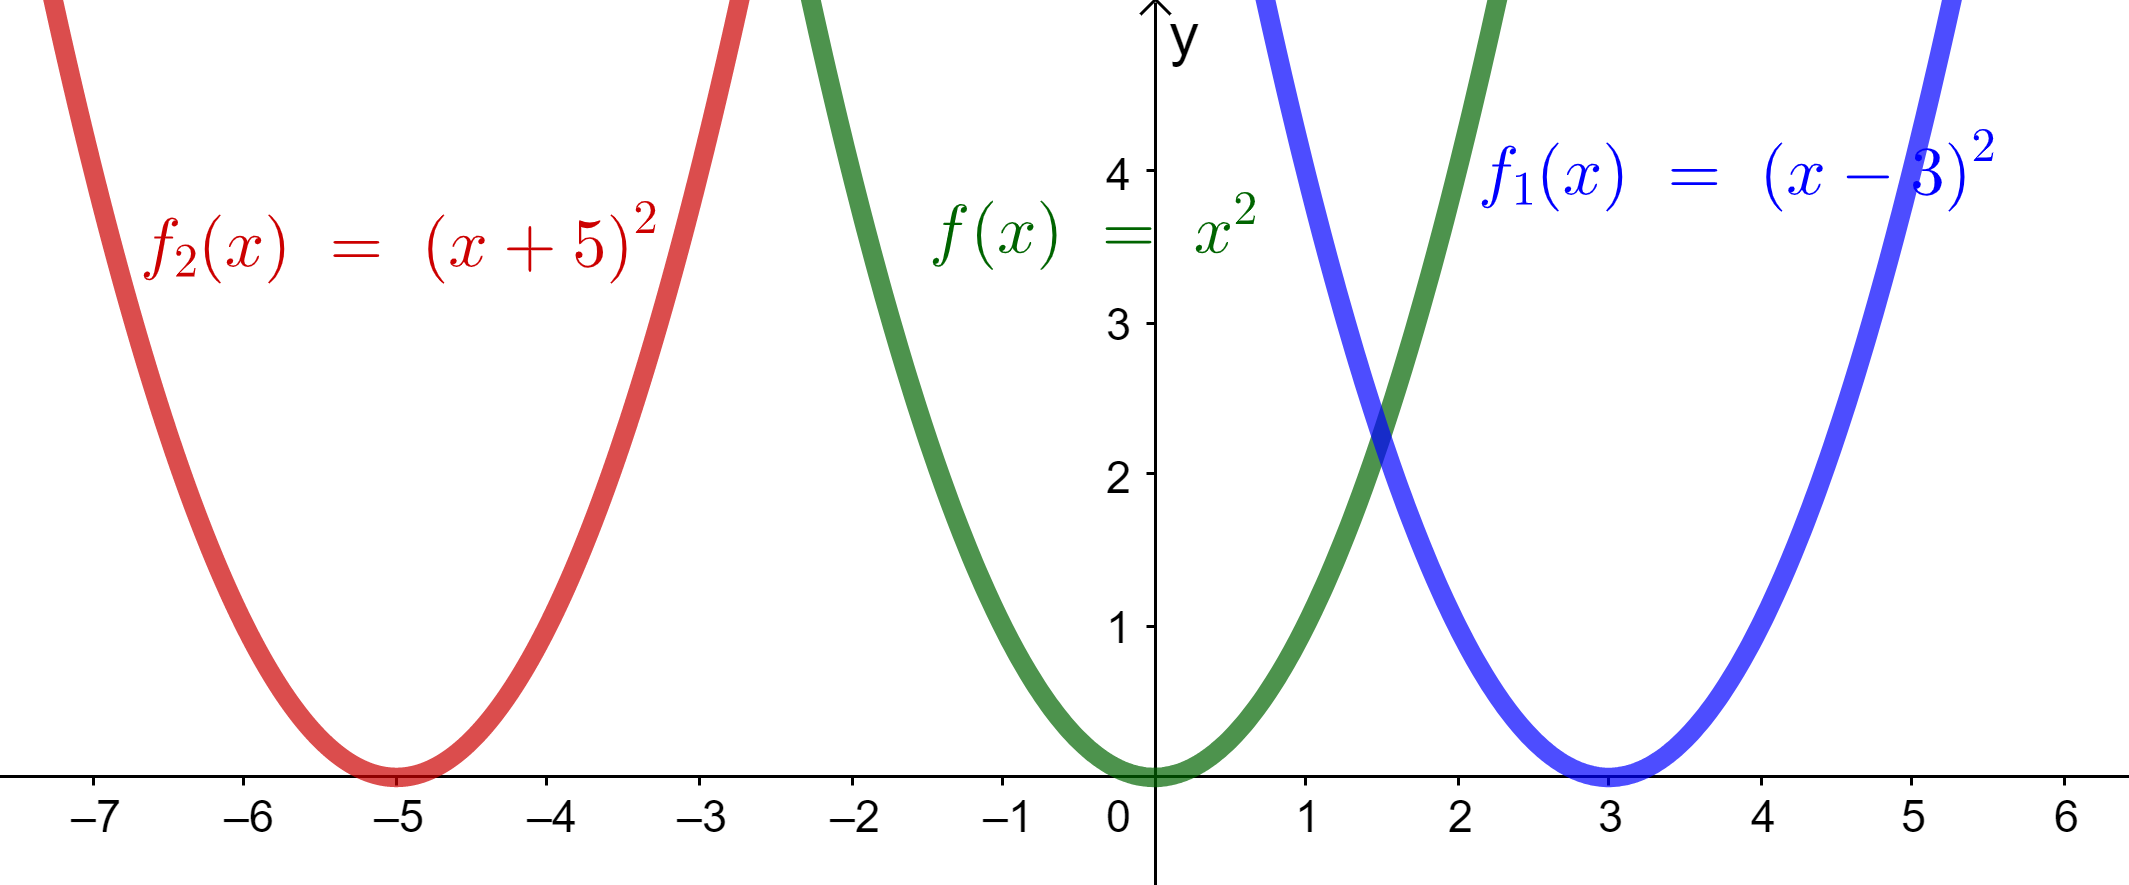
\includegraphics[width=0.95\textwidth]{../Mathematik_1/Bilder/funktionen_horizontale_verschiebung_quadratfunktion.png}
    \end{minipage}
    \begin{minipage}{0.5\textwidth}
        \begin{itemize}
            \item Originalfunktion:
            \[
            \textcolor{darkgreen}{f:x\mapsto x^2}
            \]

            \item Verschiebung um \(3\) Einheiten nach rechts:
            \[
            \textcolor{blue}{f_1:x\mapsto(x-3)^2}
            =
            \textcolor{darkgreen}{f}(x-3)
            \]

            \item Verschiebung um \(5\) Einheiten nach links:
            \[
            \textcolor{red}{f_2:x\mapsto(x+5)^2}
            =
            \textcolor{darkgreen}{f}(x+5)
            \]
        \end{itemize}
    \end{minipage}
\end{exabox}

Auch eine Multiplikation innerhalb des Arguments wirkt horizontal.
Bei
\[
x\mapsto f(kx)
\]
muss f�r einen urspr�nglich an der Stelle \(x_0\) angenommenen Funktionswert
nun
\[
kx=x_0
\]
gelten. Daraus folgt
\[
x=\frac{x_0}{k}.
\]
Die \(x\)-Koordinaten werden also mit dem Faktor \(1/k\) skaliert. Daher gilt:
\begin{itemize}
    \item F�r \(|k|>1\) wird der Graph zur \(y\)-Achse hin gestaucht.
    \item F�r \(0<|k|<1\) wird der Graph von der \(y\)-Achse weg gestreckt.
    \item F�r \(k<0\) erfolgt zus�tzlich eine Spiegelung an der \(y\)-Achse.
\end{itemize}

\begin{exabox}{Horizontale Streckung und Stauchung}{ }
    \begin{minipage}{0.4\textwidth}
        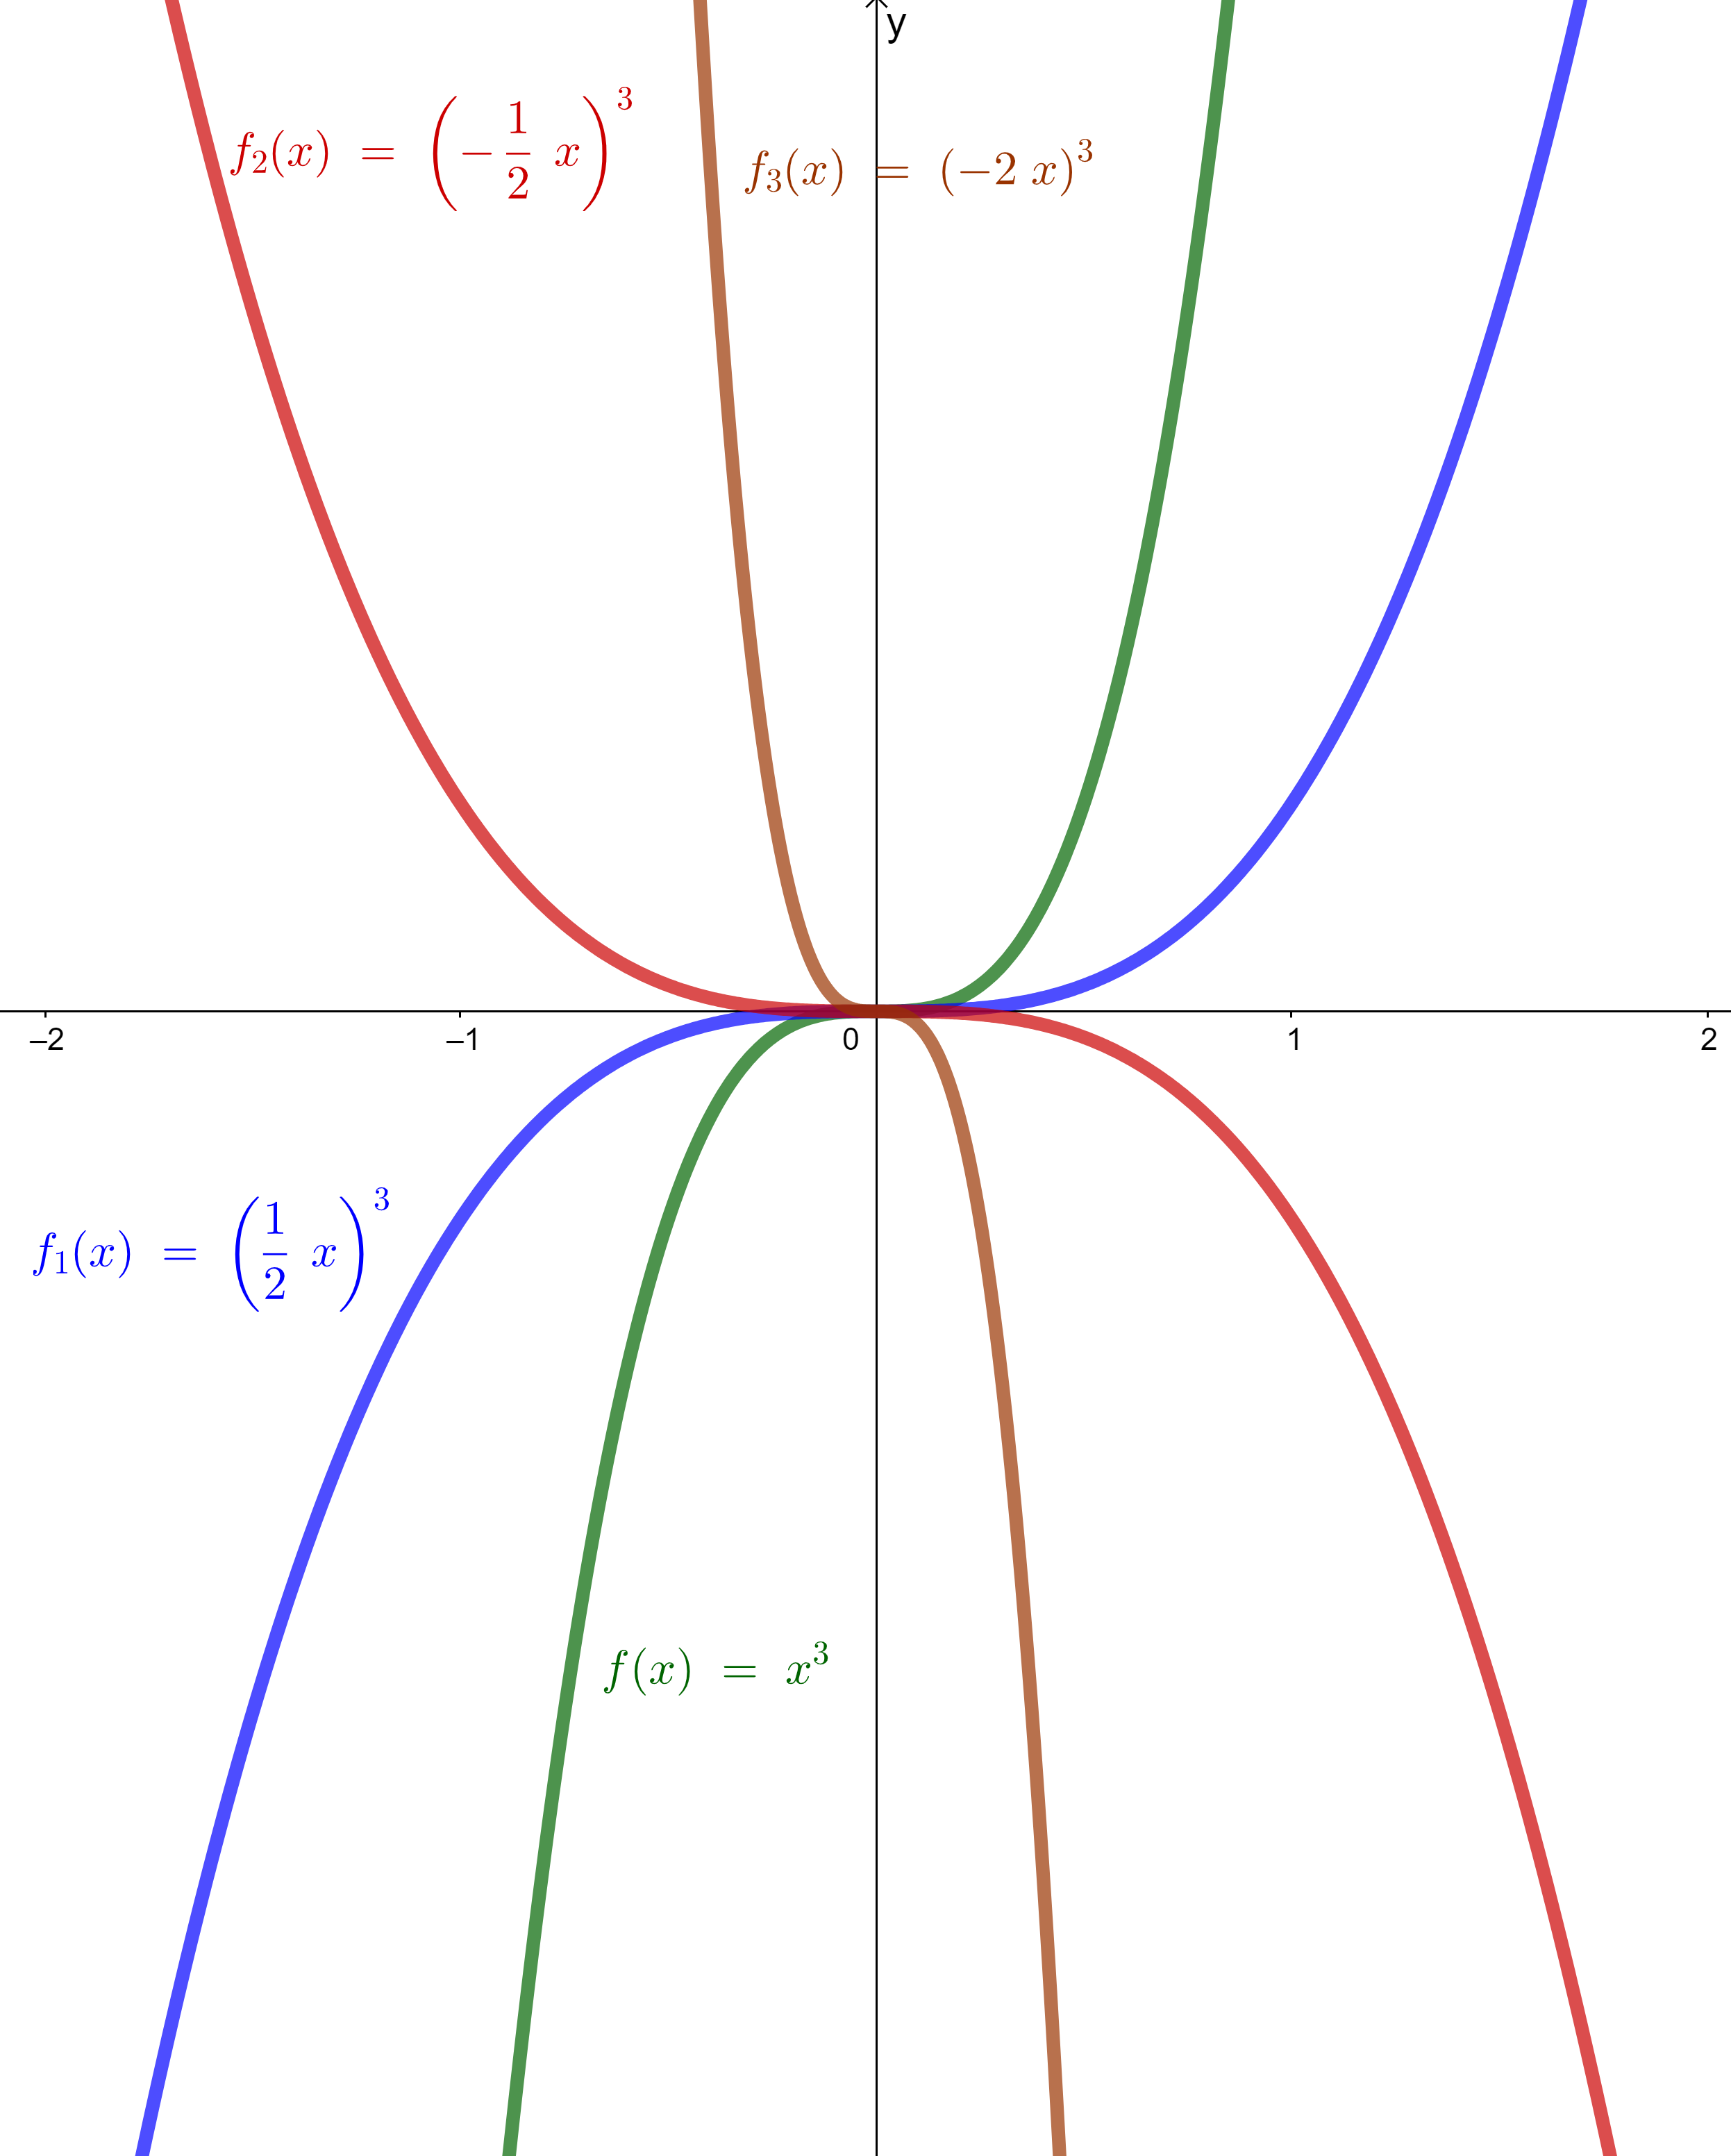
\includegraphics[width=0.95\textwidth]{../Mathematik_1/Bilder/funktionen_horizontale_skalierung_potenz_drei.png}
    \end{minipage}
    \begin{minipage}{0.6\textwidth}
        \begin{itemize}
            \item Originalfunktion:
            \[
            \textcolor{darkgreen}{f:x\mapsto x^3}
            \]

            \item Streckung in \(x\)-Richtung:
            \[
            \textcolor{blue}{
            f_1:x\mapsto
            \left(\frac12x\right)^3}
            =
            \textcolor{darkgreen}{f}\left(\frac12x\right)
            \]

            \item Streckung in \(x\)-Richtung und Spiegelung an der
            \(y\)-Achse:
            \[
            \textcolor{red}{
            f_2:x\mapsto
            \left(-\frac12x\right)^3}
            =
            \textcolor{darkgreen}{f}\left(-\frac12x\right)
            \]

            \item Stauchung in \(x\)-Richtung und Spiegelung an der
            \(y\)-Achse:
            \[
            \textcolor{brown}{
            f_3:x\mapsto(-2x)^3}
            =
            \textcolor{darkgreen}{f}(-2x)
            \]
        \end{itemize}
    \end{minipage}
\end{exabox}

Horizontale Ver�nderungen wirken damit in gewisser Weise umgekehrt zu
vertikalen Ver�nderungen: Ein Faktor mit Betrag gr��er als \(1\) f�hrt
horizontal zu einer Stauchung, ein Faktor mit Betrag kleiner als \(1\) zu
einer Streckung. Auch bei Verschiebungen erscheint das Vorzeichen innerhalb
des Funktionsarguments entgegengesetzt zur geometrischen
Verschiebungsrichtung.

Beide horizontalen Ver�nderungen lassen sich wiederum kombinieren. F�r
\[
g(x)=k(x+a),
\qquad k\neq0,
\]
gilt
\[
(f\circ g)(x)=f\!\bigl(k(x+a)\bigr).
\]

\subsubsection*{Transformationsbaukasten}

Vertikale und horizontale Ver�nderungen k�nnen gleichzeitig auftreten.
Ausgehend von einer Funktion \(f\) lassen sie sich in der Form
\[
F(x)=m\cdot f\!\bigl(k(x+a)\bigr)+b
\]
zusammenfassen.

\begin{theorembox}{Transformations-Baukasten}{ }

F�r
\[
F(x)=m\cdot f\!\bigl(k(x+a)\bigr)+b,
\qquad
m,a,b,k\in\mathbb R,\quad k\neq0,
\]
haben die Parameter folgende geometrische Bedeutung:

\begin{itemize}
		\item \(m\) ver�ndert die Funktionswerte und damit die vertikale Skalierung:
\begin{itemize}
    \item \(|m|>1\): vertikale Streckung,
    \item \(0<|m|<1\): vertikale Stauchung,
    \item \(m<0\): zus�tzliche Spiegelung an der \(x\)-Achse,
    \item \(m=0\): alle Funktionswerte werden auf \(0\) abgebildet.
\end{itemize}

    \item \(b\) verschiebt den Graphen vertikal:
          \begin{itemize}
              \item \(b>0\): nach oben,
              \item \(b<0\): nach unten.
          \end{itemize}

    \item \(k\) ver�ndert das Argument und damit die horizontale Skalierung:
          \begin{itemize}
              \item \(|k|>1\): horizontale Stauchung,
              \item \(0<|k|<1\): horizontale Streckung,
              \item \(k<0\): zus�tzliche Spiegelung an der \(y\)-Achse.
          \end{itemize}

    \item \(a\) verschiebt den Graphen horizontal:
          \begin{itemize}
              \item \(a>0\): um \(a\) Einheiten nach links,
              \item \(a<0\): um \(|a|\) Einheiten nach rechts.
          \end{itemize}
\end{itemize}

Die �u�ere Ver�nderung
\[
y\mapsto my+b
\]
wirkt auf die Funktionswerte und damit in vertikaler Richtung. Die innere
Ver�nderung
\[
x\mapsto k(x+a)
\]
wirkt auf das Argument der Funktion und damit in horizontaler Richtung.

\end{theorembox}


\subsection{Harmonische Schwingungen als Verkn�pfungen}

Die zuvor untersuchten Transformationen k�nnen nun auf die Sinusfunktion angewendet werden. Ausgehend von
\[
t\mapsto\sin(t)
\]
kann das Argument durch
\[
t\mapsto\omega\cdot  t+\varphi_0
\]
ver�ndert werden. Anschlie�end k�nnen die entstehenden Funktionswerte skaliert und verschoben werden:
\[
y\mapsto A\cdot y+d.
\]

Die Verkettung dieser drei Funktionen f�hrt auf eine \emph{harmonische Schwingung}
\[
	s(t)=A\sin(\omega t+\varphi_0)+d\,.
\]
Harmonische Schwingungen treten h�ufig auf und die Parameter besitzten eine klare Bedeutung:

\begin{itemize}
  \item \(A\not=0\) ist die \textbf{Amplitude}. F�r \(A<0\) kommt eine Spiegelung an der horizontalen Mittellinie hinzu.
  \item \(\omega>0\) ist die \textbf{Kreisfrequenz}. Sie bestimmt die \textbf{Periodendauer} \( T=\frac{2\pi}{|\omega|}\).
  \item \(\varphi_0\) ist die \textbf{Nullsphase}. Da \(\omega\neq0\) kann \( \omega t+\varphi_0 = \omega\left(t+\frac{\varphi_0}{\omega}\right) \) geschrieben werden. Dies entspricht einer horizontalen Verschiebung um \( -\frac{\varphi_0}{\omega}\).
  \item \(d\) verschiebt die Schwingung vertikal. Die Gerade \(y=d\) bildet die Mittellinie der Schwingung.
\end{itemize}

\begin{exabox}{Parameter einer harmonischen Schwingung interpretieren}{ }

Betrachtet wird die harmonische Schwingung
\[
s(t)
=
2\sin\left(3t-\frac{\pi}{2}\right)+1.
\]

Um die geometrische Bedeutung der einzelnen Parameter zu erkennen, wird die
Funktion mit der allgemeinen Form
\[
s(t)
=
A\sin(\omega t+\varphi_0)+d
\]
verglichen.

F�r die Amplitude gilt
\[
A=2.
\]
Die Schwingung besitzt daher die \textbf{Amplitude}
\[
|A|=2.
\]
Ausgehend von der Mittellinie liegen die gr��ten und kleinsten Funktionswerte
somit jeweils \(2\) Einheiten entfernt.

Die Kreisfrequenz betr�gt
\[
\omega=3.
\]
Damit ergibt sich die Periodendauer zu
\[
T
=
\frac{2\pi}{\omega}
=
\frac{2\pi}{3}.
\]
Nach einer Zeitspanne von \(2\pi/3\) wiederholt sich die Schwingung.

F�r die horizontale Verschiebung wird das Argument der Sinusfunktion
umgeformt:
\[
3t-\frac{\pi}{2}
=
3\left(t-\frac{\pi}{6}\right).
\]
Die Funktion kann daher auch in der Form
\[
s(t)
=
2\sin\left(
3\left(t-\frac{\pi}{6}\right)
\right)+1
\]
geschrieben werden. Der Graph der Sinusfunktion ist somit um
\[
\frac{\pi}{6}
\]
nach rechts verschoben.

Schlie�lich gilt
\[
d=1.
\]
Die gesamte Schwingung ist daher um eine Einheit nach oben verschoben. Ihre
Mittellinie ist
\[
y=1.
\]

Damit lassen sich die charakteristischen Eigenschaften der Schwingung
zusammenfassen:
\[
\begin{aligned}
\text{Amplitude:}\qquad &2,\\
\text{Periodendauer:}\qquad &\frac{2\pi}{3},\\
\text{horizontale Verschiebung:}\qquad &\frac{\pi}{6}\text{ nach rechts},\\
\text{Mittellinie:}\qquad &y=1.
\end{aligned}
\]

Aus der Mittellinie \(y=1\) und der Amplitude \(2\) folgen au�erdem unmittelbar
der maximale und der minimale Funktionswert:
\[
s_{\max}=1+2=3,
\qquad
s_{\min}=1-2=-1.
\]

Das Beispiel zeigt, wie die Parameter einer harmonischen Schwingung
systematisch aus ihrer Funktionsgleichung gelesen und als Ver�nderungen der
Grundfunktion \(t\mapsto \sin(t)\) interpretiert werden k�nnen.

\end{exabox}

\noindent \textbf{Merke:} 
Das Beispiel der harmonischen Schwingung zeigt, wie aus einer einfachen
Grundfunktion durch Verkettungen eine andere Funktion entsteht.

Die Verkettung von Funktionen ist damit nicht nur eine formale Operation.
Sie erm�glicht, komplexere Funktionen aus einfachen Grundfunktionen
systematisch aufzubauen und die Wirkung einzelner Parameter auf den
Funktionsgraphen zu verstehen. Diese Sichtweise wird sp�ter insbesondere bei
der Differentialrechnung wieder wichtig, wenn verkettete Funktionen mithilfe
der Kettenregel abgeleitet werden.

 \newpage % Kompositionen (inklusive harmonische Schwingungen)
\setcounter{exercise}{0} 
%\begin{exercisebox}[Verkettung]  %Moodle
%	Wenn $b\circ c$ die Funktion $2\cdot c + b$ ist, welche Funktion muss dann $b$ bezeichnen, damit $b\circ c = c\circ b$ ?
%\end{exercisebox}


\ifintegriereaufgaben
\section*{Komposition von Funktionen Aufgaben}\label{MA1-verkettung-von-funktionen-aufgaben}

	Regeln und Beispiele, die zur Bearbeitung der Aufgaben hilfreich sind, finden Sie im Skript\wennreferenzvorhanden{MA1-verkettung-von-funktionen}{ (Abschnitt \abschnittsverweis{MA1-verkettung-von-funktionen})} und, falls Sie nicht weiterkommen, schauen Sie \hyperref[MA1-verkettung-von-funktionen-loesungen]{hier}.
\else
\section{Komposition von Funktionen Aufgaben}\label{MA1-verkettung-von-funktionen-aufgaben}

	Regeln und Beispiele, die zur Bearbeitung der Aufgaben hilfreich sind, finden Sie im Skript und, falls Sie nicht weiterkommen, schauen Sie \hyperref[MA1-verkettung-von-funktionen-loesungen]{hier}.
\fi 

\begin{exercisebox}[Verkettungen]
	Bestimmen Sie Funktionen $u_1, u_2$ so, dass $f=u_1\circ v_1 = u_2\circ v_2$ ist:
  \begin{itemize}
    \item[(a)] $f(x) = (2x+6)^3, \quad v_1(x) = 2x+6, \quad v_2(x) = x+3$
    \item[(b)] $f(x) = \frac{3}{(x-1)^2}, \quad v_1(x) = x-1, \quad v_2(x) = (x-1)^2$
  \end{itemize}
\end{exercisebox}

\begin{exercisebox}[Definitionsbereich]
  Geben Sie den maximalen Definitionsbereich der Funktion $u\circ v$ an
  \begin{eqnarray*}
    (a)\; u(x) = \sqrt{x}, \quad v(x) = 3-x \quad\quad
    (b)\; u(x) = \frac{1}{x}, \quad v(x) = 4-x^2 \quad\quad
    (c)\; u(x) = \sqrt{1-x}, \quad v(x) = x^2 
  \end{eqnarray*}
\end{exercisebox}

\begin{exercisebox}[Definitionsbereich]
	Gegeben sind die Funktionen $v: \mathbb R^+ \to \mathbb R,\; x\mapsto \ln(x)$ und $u:[0,2\pi] \to \mathbb [-1,1], \,x\mapsto \sin(x)$. Betrachten Sie die Funktion $f:v \circ u$. Geben Sie den maximalen Definitionsbereich von $f$ an. 
\end{exercisebox}

\begin{exercisebox}[\(g: x\mapsto 0,7\cdot (x+2)^{-2}+4\)]
	Gegeben sind die Funktionen $f:x\mapsto x^{-2}$ und $g:x\mapsto 0,7\cdot (x+2)^{-2} +4$.
	\begin{itemize}
		\item[(a)] Geben Sie den Definitions- und den Bildbereich der Funktionen $f$ und $g$ an. 
		\item[(b)] Beschreiben Sie, wie die Funktion $g$ aus der Funktion $f$ hervorgeht. 
		\item[(c)] Bestimmen Sie die Asymptoten der Funktionen $f$ und $g$.
	\end{itemize}
\end{exercisebox}

\begin{exercisebox}[Manipulationen eines Graphen]
	Gegeben sei eine Funktion $f:\mathbb R \to \mathbb R, x\mapsto f(x)$. Geben Sie eine Abbildungsvorschrift an, um den Graphen von $f$ \dots
	\begin{itemize}
		\item[(a)] um den Faktor $5$ horizontal zu stauchen,
		\item[(b)] um den Faktor $\pi$ vertikal zu strecken,
		\item[(c)] um $2$ L�ngeneinheiten horizontal nach links zu verschieben,
		\item[(d)] um $3\sqrt{7}$ L�ngeneinheiten vertikal nach oben zu verschieben.
		\item[(e)] um den Graphen an der $x$-Achse zu spiegeln.
	\end{itemize}
\end{exercisebox}

\begin{exercisebox}[Anwendung: Temperaturskalen]
  Temperaturangaben der Kelvin Skala rechnet man in solche der Celsius Skala nach der Vorschrift $x\mapsto x- 273$ um, solche der Celsius Skala in die Fahrenheit Skala durch $x\mapsto 1,8x+32$. Wie lautet die Vorschrift, um von der Kelvin Skala direkt in die Fahrenheit Skala umzurechnen?
\end{exercisebox}
 \newpage 
\setcounter{satz}{0} \setcounter{def}{0} \setcounter{exa}{0}  \section{Komplexe Zahlen I: Zahl, Ebene und Rechnen}\label{MA1-komplexe-zahlen-grundlagen}

\begin{table}[H]
  \centering
  \begin{tabularx}{\textwidth}{p{0.9\textwidth} p{0.1\textwidth}}
    \toprule
    \multicolumn{2}{c}{\textbf{�bersicht �ber Lernziele und Voraussetzungen}}\\
    \midrule
    \textbf{Lernziele} &\\[.5\normalbaselineskip]
    \tabitem erkl�ren, warum zur L�sung bestimmter Gleichungen die komplexen Zahlen eingef�hrt werden &\\
    \tabitem komplexe Zahlen in der Form \(z=a+i\,b\) darstellen und ihre Bestandteile bestimmen &\\
    \tabitem Realteil, Imagin�rteil, komplex Konjugiertes und Betrag einer komplexen Zahl bestimmen und geometrisch interpretieren &\\
    \tabitem komplexe Zahlen als Punkte oder Pfeile in der Gau�schen Zahlenebene interpretieren &\\
    \tabitem zwischen kartesischer Darstellung und Polarkoordinaten einer komplexen Zahl wechseln &\\
    \tabitem komplexe Zahlen addieren, subtrahieren, multiplizieren und dividieren &\\
    \tabitem die geometrische Bedeutung der Grundrechenarten als Pfeiladdition, Skalierung und Drehung erkl�ren &\\[.5\normalbaselineskip]
    \midrule
    \textbf{Voraussetzungen} &\\[.5\normalbaselineskip]
    \tabitem algebraische Gleichungen und �quivalenzumformungen & \abschnittsverweis{MA1-algebraische-gleichungen}\\
    \tabitem Satz des Pythagoras und trigonometrische Funktionen & \abschnittsverweis{MA1-trigonometrische-funktionen}\\
    \tabitem kartesische Koordinaten und Polarkoordinaten & \abschnittsverweis{MA1-trigonometrische-funktionen}\\
    \bottomrule
  \end{tabularx}
\end{table}

\ifintegriereaufgaben
\noindent �bungsaufgaben zu diesem Abschnitt:
\hyperref[MA1-komplexe-zahlen-grundlagen-aufgaben]{Aufgaben}
\vspace{0.3cm}
\hrule
\fi


\subsection{Warum komplexe Zahlen?}

Die bisher betrachteten Zahlenmengen sind im Verlauf der Mathematik immer
wieder erweitert worden. In den nat�rlichen Zahlen ist beispielsweise die
Subtraktion nicht uneingeschr�nkt m�glich; die ganzen Zahlen schlie�en diese
L�cke. In den ganzen Zahlen ist die Division nicht uneingeschr�nkt m�glich;
die rationalen Zahlen erweitern den Zahlenbereich entsprechend. Die reellen
Zahlen erm�glichen schlie�lich unter anderem die Beschreibung irrationaler
Gr��en wie \(\sqrt{2}\).

Auch innerhalb der reellen Zahlen bleiben jedoch Gleichungen �brig, die keine
L�sung besitzen. Das einfachste Beispiel ist
\[
x^2=-1.
\]
F�r jede reelle Zahl \(x\) gilt
\[
x^2\geq0.
\]
Daher kann keine reelle Zahl die Gleichung \(x^2=-1\) erf�llen.

Um auch solche Gleichungen behandeln zu k�nnen, wird der Zahlenbereich erneut
erweitert.

\begin{defbox}{Imagin�re Einheit}{ }

Die \textbf{imagin�re Einheit} (\emph{imaginary unit}) \(i\) ist durch
\[
i^2=-1
\]
definiert.

Damit besitzt die Gleichung
\[
x^2=-1
\]
in den komplexen Zahlen die beiden L�sungen
\[
x=\pm i.
\]

\end{defbox}

In der Elektrotechnik wird f�r die imagin�re Einheit h�ufig \(j\) anstelle
von \(i\) verwendet, da \(i\) dort �blicherweise die elektrische Stromst�rke
bezeichnet.

Eine \textbf{komplexe Zahl} (\emph{complex number}) entsteht, indem zu einer
reellen Zahl ein reelles Vielfaches der imagin�ren Einheit addiert wird:
\[
z=a+i\,b,
\qquad
a,b\in\mathbb R.
\]

Die Menge aller komplexen Zahlen wird mit
\[
\mathbb C
=
\{a+i\,b:a,b\in\mathbb R\}
\]
bezeichnet.

F�r \(b=0\) ergibt sich
\[
z=a+i\cdot0=a.
\]
Jede reelle Zahl ist damit zugleich eine komplexe Zahl. Es gilt also
\[
\mathbb R\subset\mathbb C.
\]
Die komplexen Zahlen ersetzen die reellen Zahlen somit nicht, sondern
erweitern den bisherigen Zahlenbereich.

\begin{exabox}{Beispiele komplexer Zahlen}{ }

Beispielsweise gilt
\[
\left\{
1+3i,\;
\sqrt7-91i,\;
3\pi i,\;
0,\;
\pi+\frac{71}{13}i
\right\}
\subset\mathbb C.
\]

Dabei sind auch rein reelle Zahlen wie \(0\) sowie rein imagin�re Zahlen wie
\(3\pi i\) komplexe Zahlen.

\end{exabox}

Die Einf�hrung der komplexen Zahlen erm�glicht insbesondere die L�sung
quadratischer Gleichungen, deren Diskriminante negativ ist. Ein einfaches
Beispiel zeigt, wie komplexe L�sungen dabei entstehen.

\begin{exabox}{Eine quadratische Gleichung mit komplexen L�sungen}{ }

Betrachtet wird die Gleichung
\[
x^2-4x+5=0.
\]

Durch quadratische Erg�nzung ergibt sich
\[
\begin{array}{crcl}
                  & x^2-4x+5       &=& 0\\
\Leftrightarrow   & x^2-4x+4-4+5   &=& 0\\
\Leftrightarrow   & (x-2)^2+1      &=& 0\\
\Leftrightarrow   & (x-2)^2        &=& -1.
\end{array}
\]

Mit
\[
i^2=-1
\]
folgt
\[
x-2=\pm i
\]
und damit
\[
x_{1,2}=2\pm i.
\]

Die Gleichung besitzt keine reellen L�sungen, wohl aber die beiden komplexen
L�sungen
\[
2+i
\qquad\text{und}\qquad
2-i.
\]

\end{exabox}

\noindent\textbf{Bemerkung:}
In der Praxis kann eine quadratische Gleichung nat�rlich weiterhin mit der
allgemeinen L�sungsformel gel�st werden. Ist die \underline{Diskriminante}\randverweis{MA1-algebraische-gleichungen} negativ, f�hrt die auftretende Wurzel einer negativen Zahl auf komplexe L�sungen. Die
quadratische Erg�nzung im vorangegangenen Beispiel macht dagegen besonders
deutlich, an welcher Stelle die imagin�re Einheit \(i\) ben�tigt wird.


\subsection{Bausteine einer komplexen Zahl}

Eine komplexe Zahl
\[
z=a+i\,b
\]
besteht aus zwei reellen Komponenten. Die Zahl \(a\) beschreibt den reellen
Anteil, die Zahl \(b\) den Koeffizienten der imagin�ren Einheit.

\begin{defbox}{Grundbegriffe und Notationen}{ }

F�r
\[
z=a+i\,b,
\qquad a,b\in\mathbb R,
\]
gelten folgende Bezeichnungen:

\begin{itemize}
    \item Der \textbf{Realteil} (\emph{real part}) von \(z\) ist
    \[
    \mathrm{Re}(z)=a.
    \]

    \item Der \textbf{Imagin�rteil} (\emph{imaginary part}) von \(z\) ist
    \[
    \mathrm{Im}(z)=b.
    \]

    \item Die \textbf{komplex konjugierte Zahl}
    (\emph{complex conjugate}) zu \(z\) ist
    \[
    \overline z=a-i\,b.
    \]

    \item Der \textbf{Betrag} (\emph{magnitude}) von \(z\) ist
    \[
    |z|
    =
    \sqrt{a^2+b^2}.
    \]
\end{itemize}

\end{defbox}

Die Begriffe lassen sich unmittelbar an einer konkreten komplexen Zahl ablesen.

\begin{exabox}{Realteil, Imagin�rteil, Konjugation und Betrag}{ }

\begin{minipage}{0.3\textwidth}
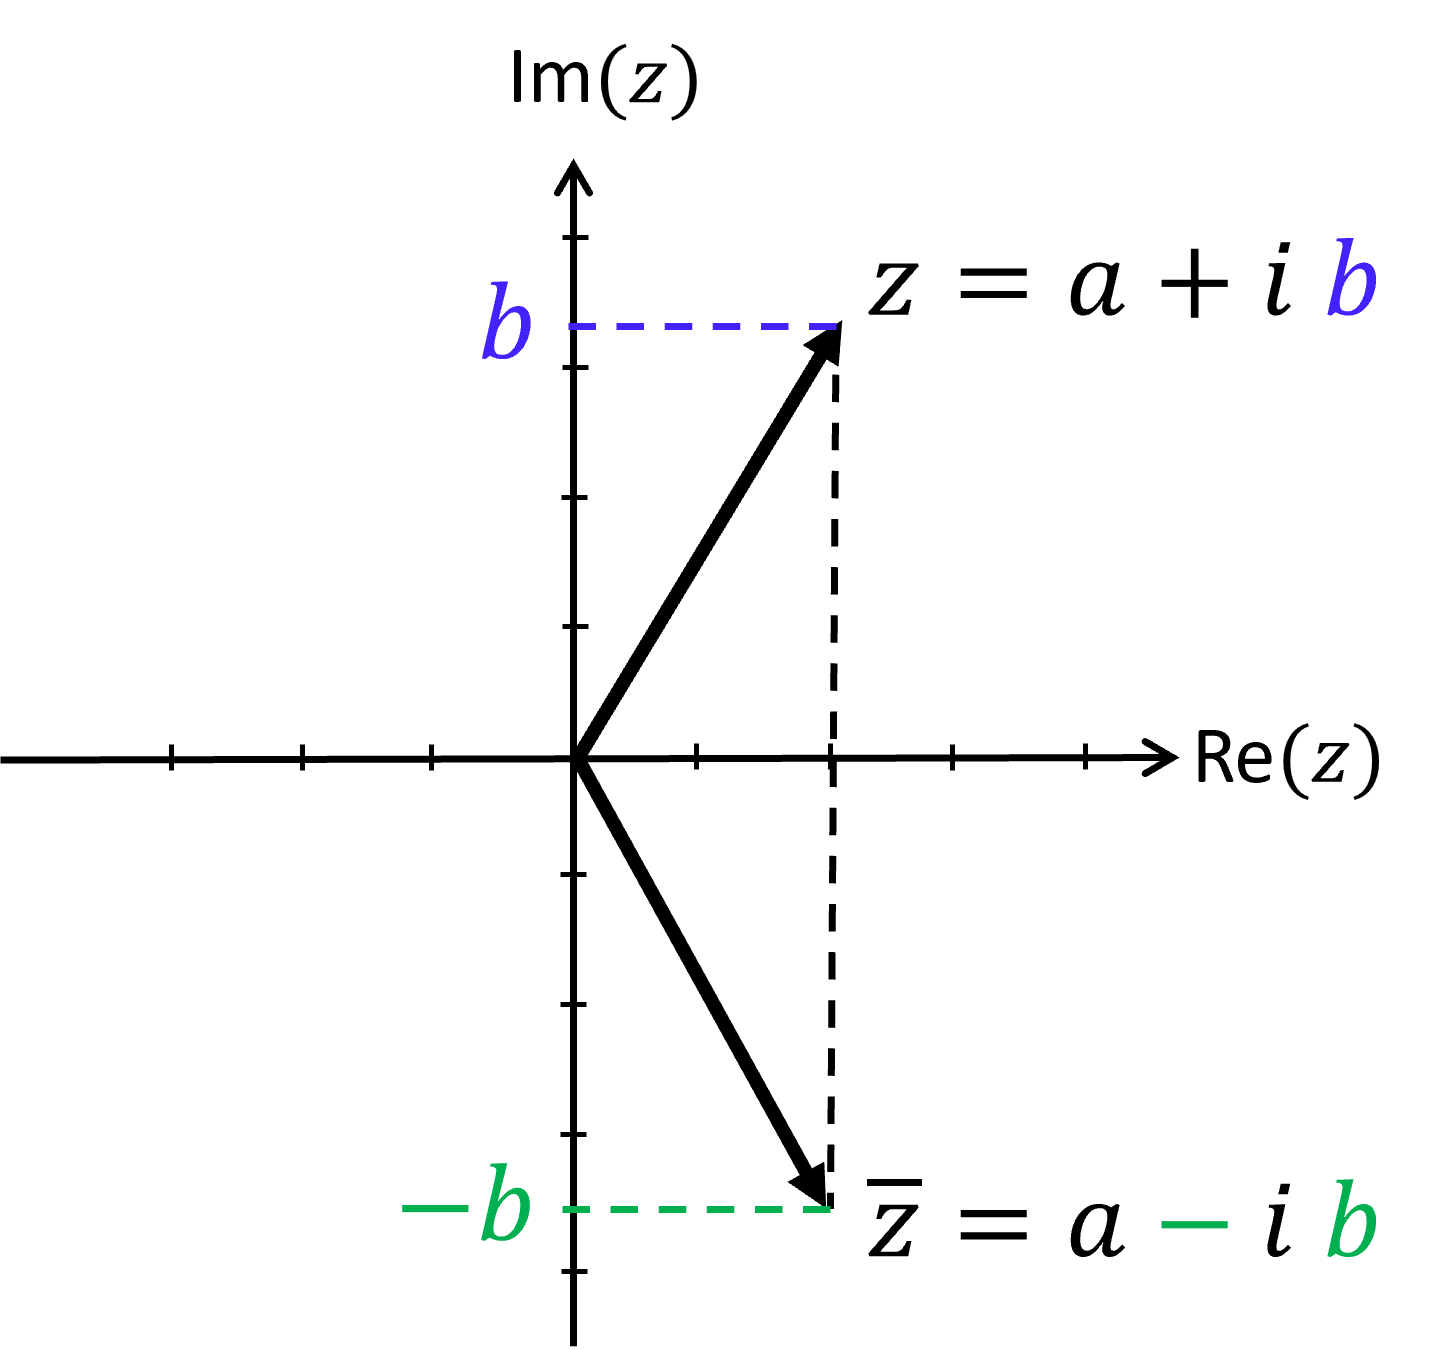
\includegraphics[width=\textwidth]{../Mathematik_1/Bilder/komplexe_zahlen_konjugation_spiegelung.png}
\end{minipage}
\begin{minipage}{0.68\textwidth}


F�r
\[
z=3+4i
\]
gilt
\[
\mathrm{Re}(z)=3
\qquad\text{und}\qquad
\mathrm{Im}(z)=4.
\]

Die komplex konjugierte Zahl lautet
\[
\overline z=3-4i.
\]

F�r den Betrag ergibt sich
\[
|z|
=
\sqrt{(\mathrm{Re}(z))^2+(\mathrm{Im}(z))^2}
=
\sqrt{3^2+4^2}
=
\sqrt{25}
=
5.
\]
\end{minipage}

\end{exabox}

Zwischen diesen Begriffen bestehen einige wichtige Zusammenh�nge. F�r
\[
z=a+i\,b
\]
gilt zun�chst
\[
|z|\geq0
\]
und
\[
|z|=0
\quad\Longleftrightarrow\quad
z=0.
\]

Ist \(z\) reell, also \(b=0\), so ergibt sich
\[
|z|
=
\sqrt{a^2}
=
|a|.
\]
Der Betrag einer komplexen Zahl erweitert damit den bereits bekannten
Absolutbetrag reeller Zahlen.

Besonders wichtig ist das Produkt einer komplexen Zahl mit ihrer konjugierten
Zahl:
\[
z\overline z
=
(a+i\,b)\cdot (a-i\,b)
=
a^2-i\, a\cdot b+i\, a\cdot b-i^2\cdot b^2
=
a^2+b^2
=
|z|^2.
\]
Damit gilt
\[
z\overline z=|z|^2
\]
und entsprechend
\[
|z|=\sqrt{z\overline z}.
\]

Au�erdem gilt
\[
z+\overline z=2\,\mathrm{Re}(z)
\]
sowie
\[
z-\overline z=2i\,\mathrm{Im}(z).
\]

Die algebraischen Begriffe erhalten eine besonders anschauliche Bedeutung,
sobald komplexe Zahlen geometrisch dargestellt werden.


\subsection{Die Gau�sche Zahlenebene}

Eine komplexe Zahl
\[
z=a+i\,b
\]
wird durch zwei reelle Zahlen \(a\) und \(b\) bestimmt. Daher liegt es nahe,
sie mit einem Punkt
\[
(a,b)\in\mathbb R^2
\]
zu identifizieren.

Im Zusammenhang mit komplexen Zahlen wird dieses Koordinatensystem als
\textbf{Gau�sche Zahlenebene} (\emph{complex plane}) bezeichnet. Die
horizontale Achse stellt den Realteil, die vertikale Achse den Imagin�rteil
dar.

Eine komplexe Zahl kann dabei entweder als Punkt oder als Pfeil vom Ursprung
zu diesem Punkt aufgefasst werden:
\[
z=a+i\,b
\quad\widehat=\quad
(a\,|\,b).
\]

\begin{theorembox}{Kartesische Darstellung}{ }

\begin{minipage}{0.3\textwidth}
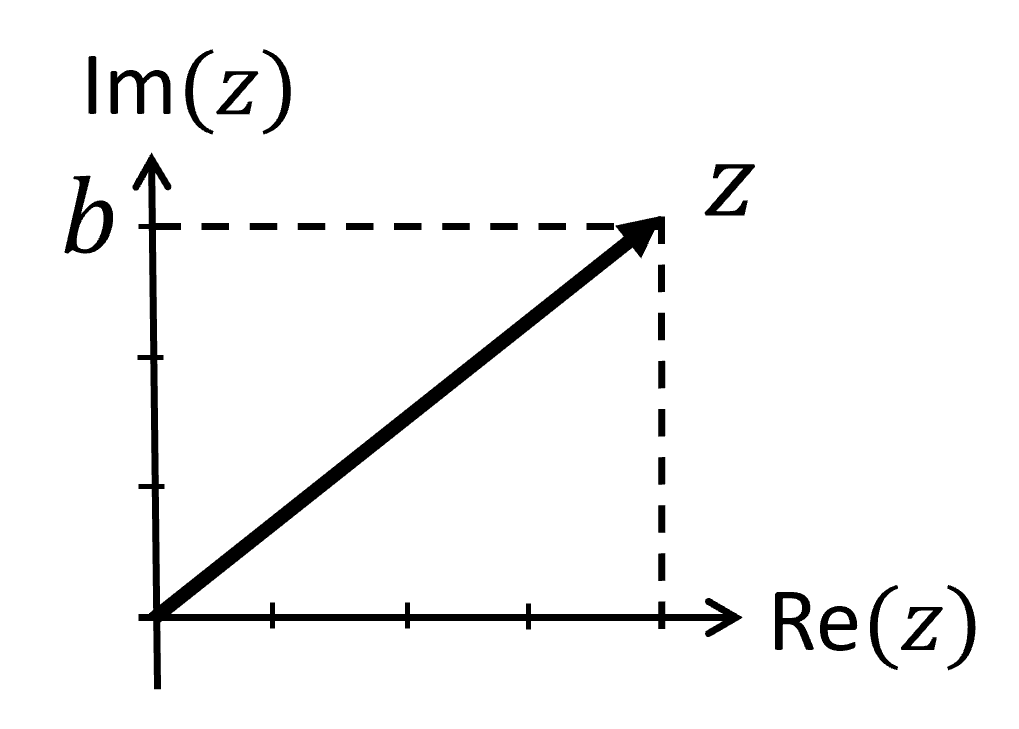
\includegraphics[width=\textwidth]{../Mathematik_1/Bilder/komplexe_zahlen_kartesische_koordinaten.png}
\end{minipage}
\begin{minipage}{0.68\textwidth}

F�r
\[
z=a+i\,b
\]
gilt
\[
z\;\widehat=\;(a\,|\,b),
\]
wobei
\[
a=\mathrm{Re}(z),
\qquad
b=\mathrm{Im}(z).
\]

Der zugeh�rige Pfeil beginnt im Ursprung und endet im Punkt
\[
(a\,|\,b).
\]

\end{minipage}

\end{theorembox}

Durch diese Darstellung erhalten auch die zuvor eingef�hrten Begriffe eine
geometrische Bedeutung.

Der Betrag
\[
|z|=\sqrt{a^2+b^2}
\]
ist nach dem Satz des Pythagoras gerade die L�nge des Pfeils vom Ursprung zum
Punkt \((a\,|\,b)\).

Die komplex konjugierte Zahl
\[
\overline z=a-i\,b
\]
entspricht dem Punkt
\[
(a\,|\,-b).
\]
Die komplexe Konjugation spiegelt den zu \(z\) geh�renden Punkt beziehungsweise
Pfeil daher an der reellen Achse.


\subsubsection*{Polarkoordinaten einer komplexen Zahl}

Die kartesischen Koordinaten beschreiben eine komplexe Zahl durch ihre
horizontale und vertikale Komponente. Derselbe Pfeil kann jedoch auch durch
seine L�nge und seine Richtung beschrieben werden.

Dazu werden der Betrag
\[
r=|z|
\]
und ein Winkel \(\varphi\) verwendet, den der Pfeil mit der positiven reellen
Achse einschlie�t. Diese Beschreibung f�hrt auf die
\textbf{Polarkoordinaten} einer komplexen Zahl.

\begin{theorembox}{Polarkoordinaten}{ }

\begin{minipage}{0.3\textwidth}
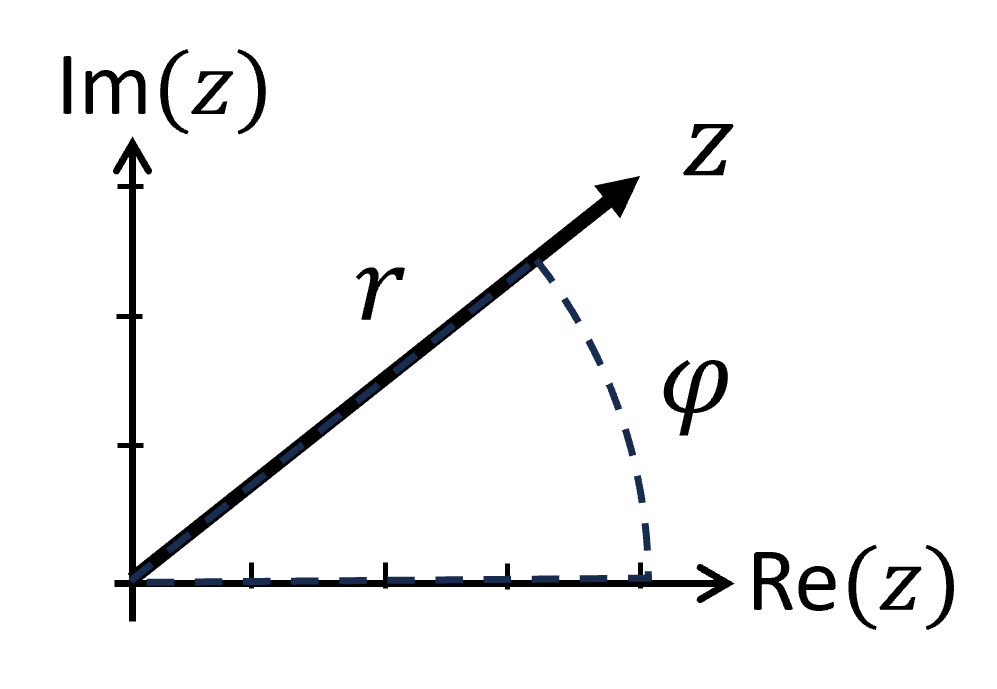
\includegraphics[width=\textwidth]{../Mathematik_1/Bilder/komplexe_zahlen_polarkoordinaten.png}
\end{minipage}
\begin{minipage}{0.7\textwidth}

F�r eine komplexe Zahl \(z\neq0\) gilt
\[
z\;\widehat=\;(r\,|\,\varphi), \quad 
\]
wobei
	\begin{itemize}
		\item \( r=|z|>0 \) die L�nge des Pfils und 
		\item \( \varphi=\arg(z) \) der Winkel zwischen Pfeil und positiven reellen Achse ist.
	\end{itemize}

\end{minipage}

\end{theorembox}

Der Winkel einer komplexen Zahl ist grunds�tzlich nur bis auf ganzzahlige
Vielfache von \(2\pi\) bestimmt. Die Winkel
\[
\varphi_k
=
\varphi+2\pi k,
\qquad k\in\mathbb Z,
\]
beschreiben daher dieselbe Richtung und somit dieselbe komplexe Zahl. Im Folgenden bezeichnet
\[
\arg(z)\in(-\pi,\pi]
\]
den gew�hlten Hauptwert des Arguments.


F�r \(z=0\) gilt zwar \(|z| = 0\), ein Winkel ist jedoch nicht eindeutig bestimmt. Das Argument von \(0\) ist daher nicht definiert.


\subsubsection*{Von Polarkoordinaten zur kartesischen Darstellung}

Sind Betrag \(r\) und Winkel \(\varphi\) gegeben, ergeben sich die
kartesischen Koordinaten unmittelbar aus der Geometrie des zugeh�rigen
rechtwinkligen Dreiecks:
\[
a=r\cos(\varphi)
\]
und
\[
b=r\sin(\varphi).
\]

Damit gilt
\[
z
=
r\cos(\varphi)
+
i\,r\sin(\varphi).
\]

Durch Ausklammern von \(r\) erh�lt man die besonders wichtige Darstellung
\[
z
=
r\bigl(\cos(\varphi)+i\sin(\varphi)\bigr).
\]

Diese Form wird im folgenden Abschnitt eine zentrale Rolle spielen, wenn die
trigonometrische Darstellung mit der komplexen Exponentialfunktion verbunden
wird.


\subsubsection*{Von der kartesischen Darstellung zu Polarkoordinaten}

Ist dagegen \( z = a + i\, b\) gegeben, so liefert der Satz des Pythagoras zun�chst den Betrag:
\[
r
=
|z|
=
\sqrt{a^2+b^2}.
\]

F�r den Winkel m�ssen beide kartesischen Koordinaten ber�cksichtigt werden.
Die Funktion
\[
\operatorname{atan2}(b,a)
\]
liefert den Winkel unter Ber�cksichtigung des Quadranten. F�r \(z\neq0\) gilt
daher
\[
\varphi
=
\operatorname{atan2}(b,a)
\in(-\pi,\pi].
\]

Damit lautet die Umrechnung insgesamt
\[
a+i\,b
\quad\longleftrightarrow\quad
\left(
\sqrt{a^2+b^2}
\,\middle|\,
\operatorname{atan2}(b,a)
\right).
\]

\begin{theorembox}{Kartesisch \(\leftrightarrow\) Polar}{ }

\begin{minipage}{0.3\textwidth}
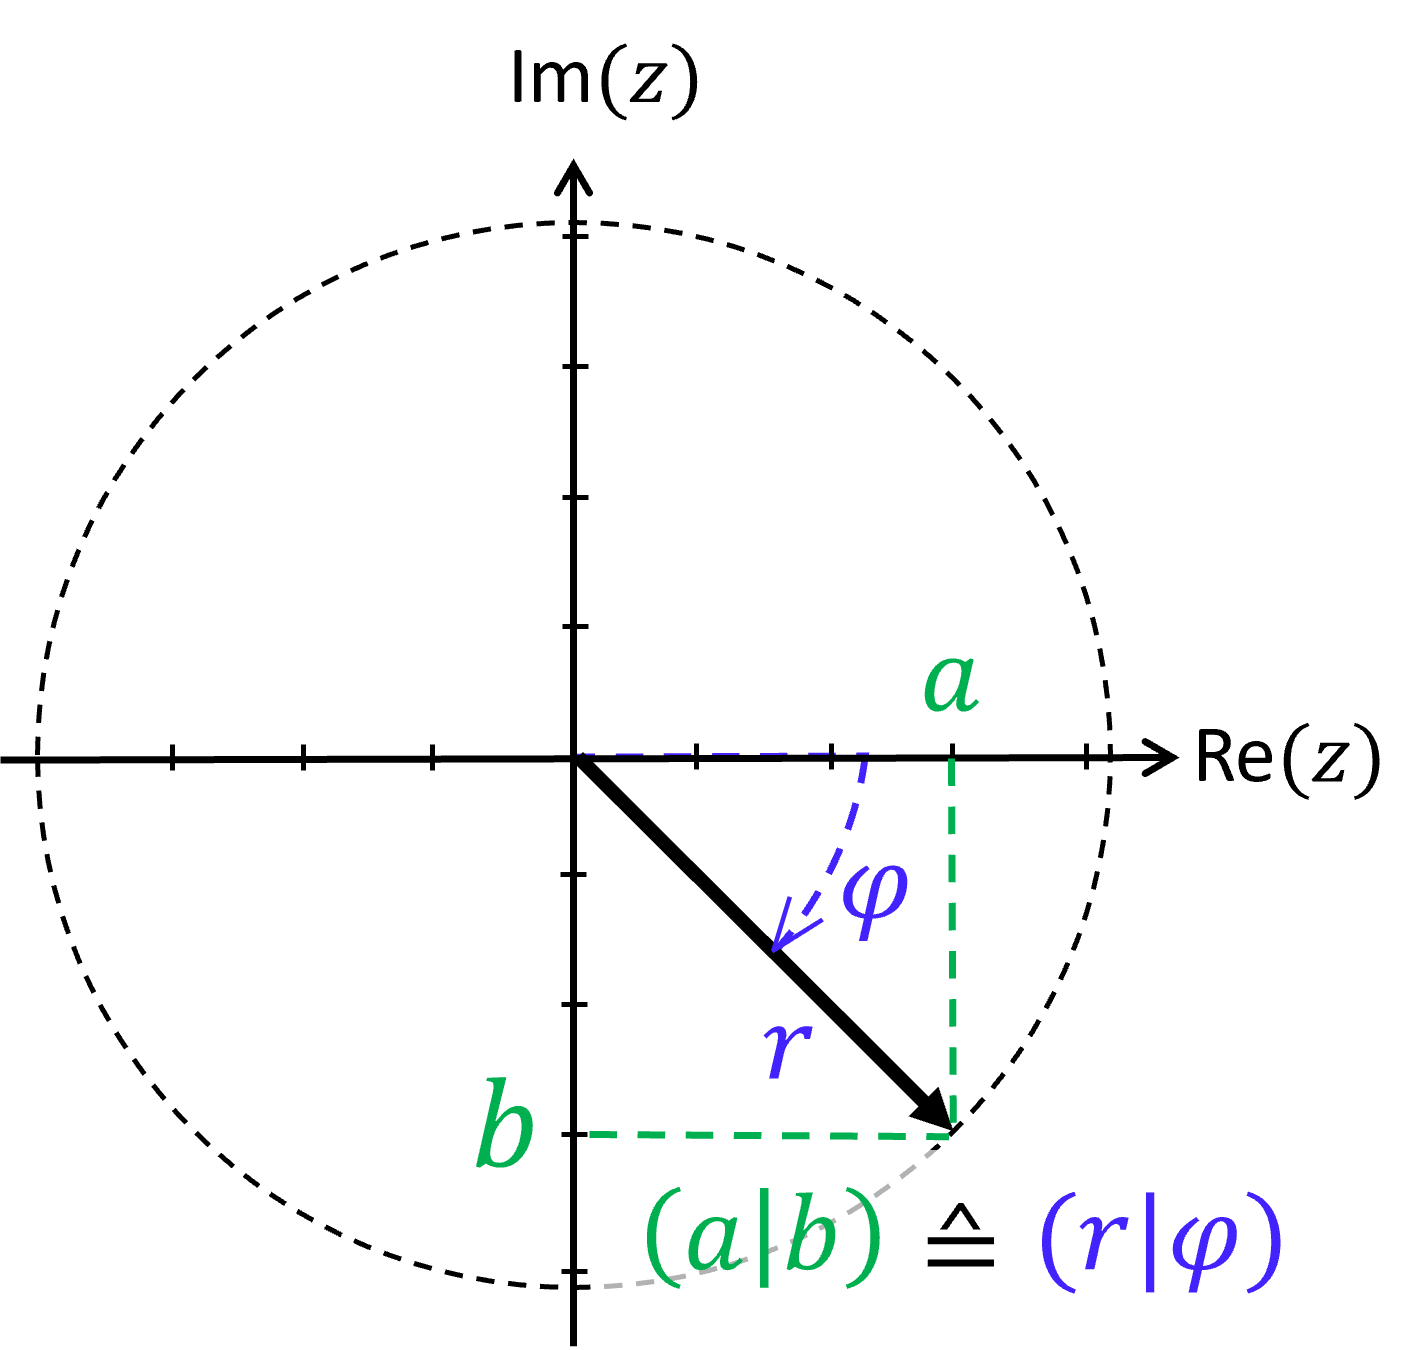
\includegraphics[width=0.8\textwidth]{../Mathematik_1/Bilder/komplexe_zahlen_kartesisch_polar_vierter_quadrant.png}
\end{minipage}
\begin{minipage}{0.7\textwidth}
	Polarkoordinaten \(\Leftrightarrow\) kartesische Koordinaten: 
	\begin{eqnarray*}
		\color{green}{a} &=& \color{blue}{r}\cdot \cos(\color{blue}{\varphi}) \\
		\color{green}{b} &=& \color{blue}{r}\cdot \sin(\color{blue}{\varphi})
	\end{eqnarray*}
kartesische Koordinaten  \(\Leftrightarrow\) 	Polarkoordinaten:
	\begin{eqnarray*}
		\color{blue}{r} &=& \sqrt{ \color{green}{a}^2 + \color{green}{b}^2} \\
		\color{blue}{\varphi} &=& \text{atan2}(\color{green}{b}, \color{green}{a}) 
	\end{eqnarray*}
\end{minipage}

\end{theorembox}

\begin{exabox}{Von kartesischen Koordinaten zu Polarkoordinaten}{ }

Betrachtet wird die komplexe Zahl
\[
z=-1+i\sqrt3.
\]

Der Betrag ergibt sich zu
\[
r = |z| = \sqrt{(-1)^2+(\sqrt3)^2} = 2
\]

Der zugeh�rige Punkt
\[
(-1\,|\,\sqrt3)
\]
liegt im zweiten Quadranten. F�r den Winkel ergibt sich
\[
\varphi
=
\operatorname{atan2}(\sqrt3,-1)
=
\frac{2\pi}{3}.
\]

Damit besitzt \(z\) die Polarkoordinaten
\[
z
\;\widehat=\;
\left(2\,\middle|\,\frac{2\pi}{3}\right).
\]

Zur Kontrolle kann wieder in die kartesische Darstellung zur�ckgerechnet
werden:
\[
\begin{aligned}
a &= 2\cos\left(\frac{2\pi}{3}\right) = 2\left(-\frac12\right) = -1,\\
b &= 2\sin\left(\frac{2\pi}{3}\right) = 2\frac{\sqrt3}{2} = \sqrt3.
\end{aligned}
\]
Damit ergibt sich tats�chlich wieder
\[
z=-1+i\sqrt3.
\]

\end{exabox}


\subsection{Rechnen in \(\mathbb C\)}

Die Darstellung \(z = a + i\, b\) erm�glicht es, komplexe Zahlen algebraisch �hnlich wie reelle Zahlen zu behandeln. Dabei wird \(i\) zun�chst wie eine algebraische Gr��e behandelt; auftretende Potenzen \(i^2\) werden anschlie�end mithilfe von \(i^2 = -1\) vereinfacht.

Bei Addition und Subtraktion werden Real- und Imagin�rteile getrennt
zusammengefasst. Bei der Multiplikation wird wie bei Klammerprodukten
ausmultipliziert. F�r die Division spielt die komplexe Konjugation eine
besondere Rolle.

\begin{exabox}{Rechnen mit komplexen Zahlen}{ }

Es seien
\[
	z_1=2+3\, i
\qquad\text{und}\qquad
z_2=4+i.
\]

Bei der Addition werden Real- und Imagin�rteile jeweils zusammengefasst:
\[
z_1+z_2
=
(2+3\,i)+(4+i)
=
(2+4)+(3+1)\,i
=
6+4\,i.
\]

F�r die Subtraktion ergibt sich entsprechend
\[
z_1-z_2
=
(2+3\,i)-(4+i)
=
(2-4)+(3-1)\,i
=
-2+2\,i.
\]

Bei der Multiplikation wird zun�chst ausmultipliziert:
\[
z_1\cdot z_2
=
(2+3\,i)\cdot (4+i)
=
8+2\,i+12\,i+3\,i^2
=
8+14\,i-3
=
5+14\,i.
\]

F�r die Division wird der Nenner mithilfe seiner komplex konjugierten Zahl
reell gemacht. Da
\[
\overline{z_2}=4-i,
\]
gilt
\[
\frac{z_1}{z_2}
=
\frac{2+3\,i}{4+i}
=
\frac{2+3\,i}{4+i}
\cdot
\frac{4-i}{4-i}
=
\frac{(2+3\,i)(4-i)}{(4+i)(4-i)}.
\]

Der Nenner wird dabei zu
\[
(4+i)\cdot (4-i)
=
4^2-i^2
=
16+1
=
17.
\]

F�r den Z�hler ergibt sich
\[
	(2+3\,i)\cdot (4-i)
=
8-2\,i+12\,i-3\,i^2
=
11+10\,i.
\]

Damit folgt
\[
\frac{z_1}{z_2}
=
\frac{11}{17}
+
\frac{10}{17}\,i.
\]

\end{exabox}

Das Vorgehen bei der Division beruht auf der bereits bekannten Beziehung
\[
z\overline z=|z|^2.
\]
F�r
\[
z_2\neq0
\]
ist daher
\[
\frac{z_1}{z_2}
=
\frac{z_1\overline{z_2}}{z_2\overline{z_2}}
=
\frac{z_1\overline{z_2}}{|z_2|^2}.
\]
Der Nenner ist damit eine positive reelle Zahl.

Die algebraischen Rechenregeln erkl�ren, wie komplexe Zahlen berechnet
werden. Die Darstellung in der Gau�schen Zahlenebene zeigt dar�ber hinaus,
welche geometrischen Operationen hinter diesen Rechnungen stehen.


\subsection{Geometrische Bedeutung der Grundrechenarten}

\subsubsection*{Addition und Subtraktion: Pfeiladdition}

Die kartesische Darstellung macht die Addition besonders anschaulich. F�r
\[
z_1=a_1+i\,b_1
\qquad\text{und}\qquad
z_2=a_2+i\,b_2
\]
gilt
\[
z_1+z_2
=
(a_1+a_2)+i\,(b_1+b_2).
\]

Damit werden genau die beiden Koordinaten der zugeh�rigen Pfeile addiert. Die
\underline{Addition komplexer Zahlen}\marginpar{\small{\href{https://www.geogebra.org/m/quynhvdx}{GeoGebra}}} entspricht daher der bekannten Addition von
Pfeilen beziehungsweise Vektoren in der Ebene.

\begin{exabox}{Addition und Subtraktion in der Zahlenebene}{ }

\begin{minipage}{0.45\textwidth}
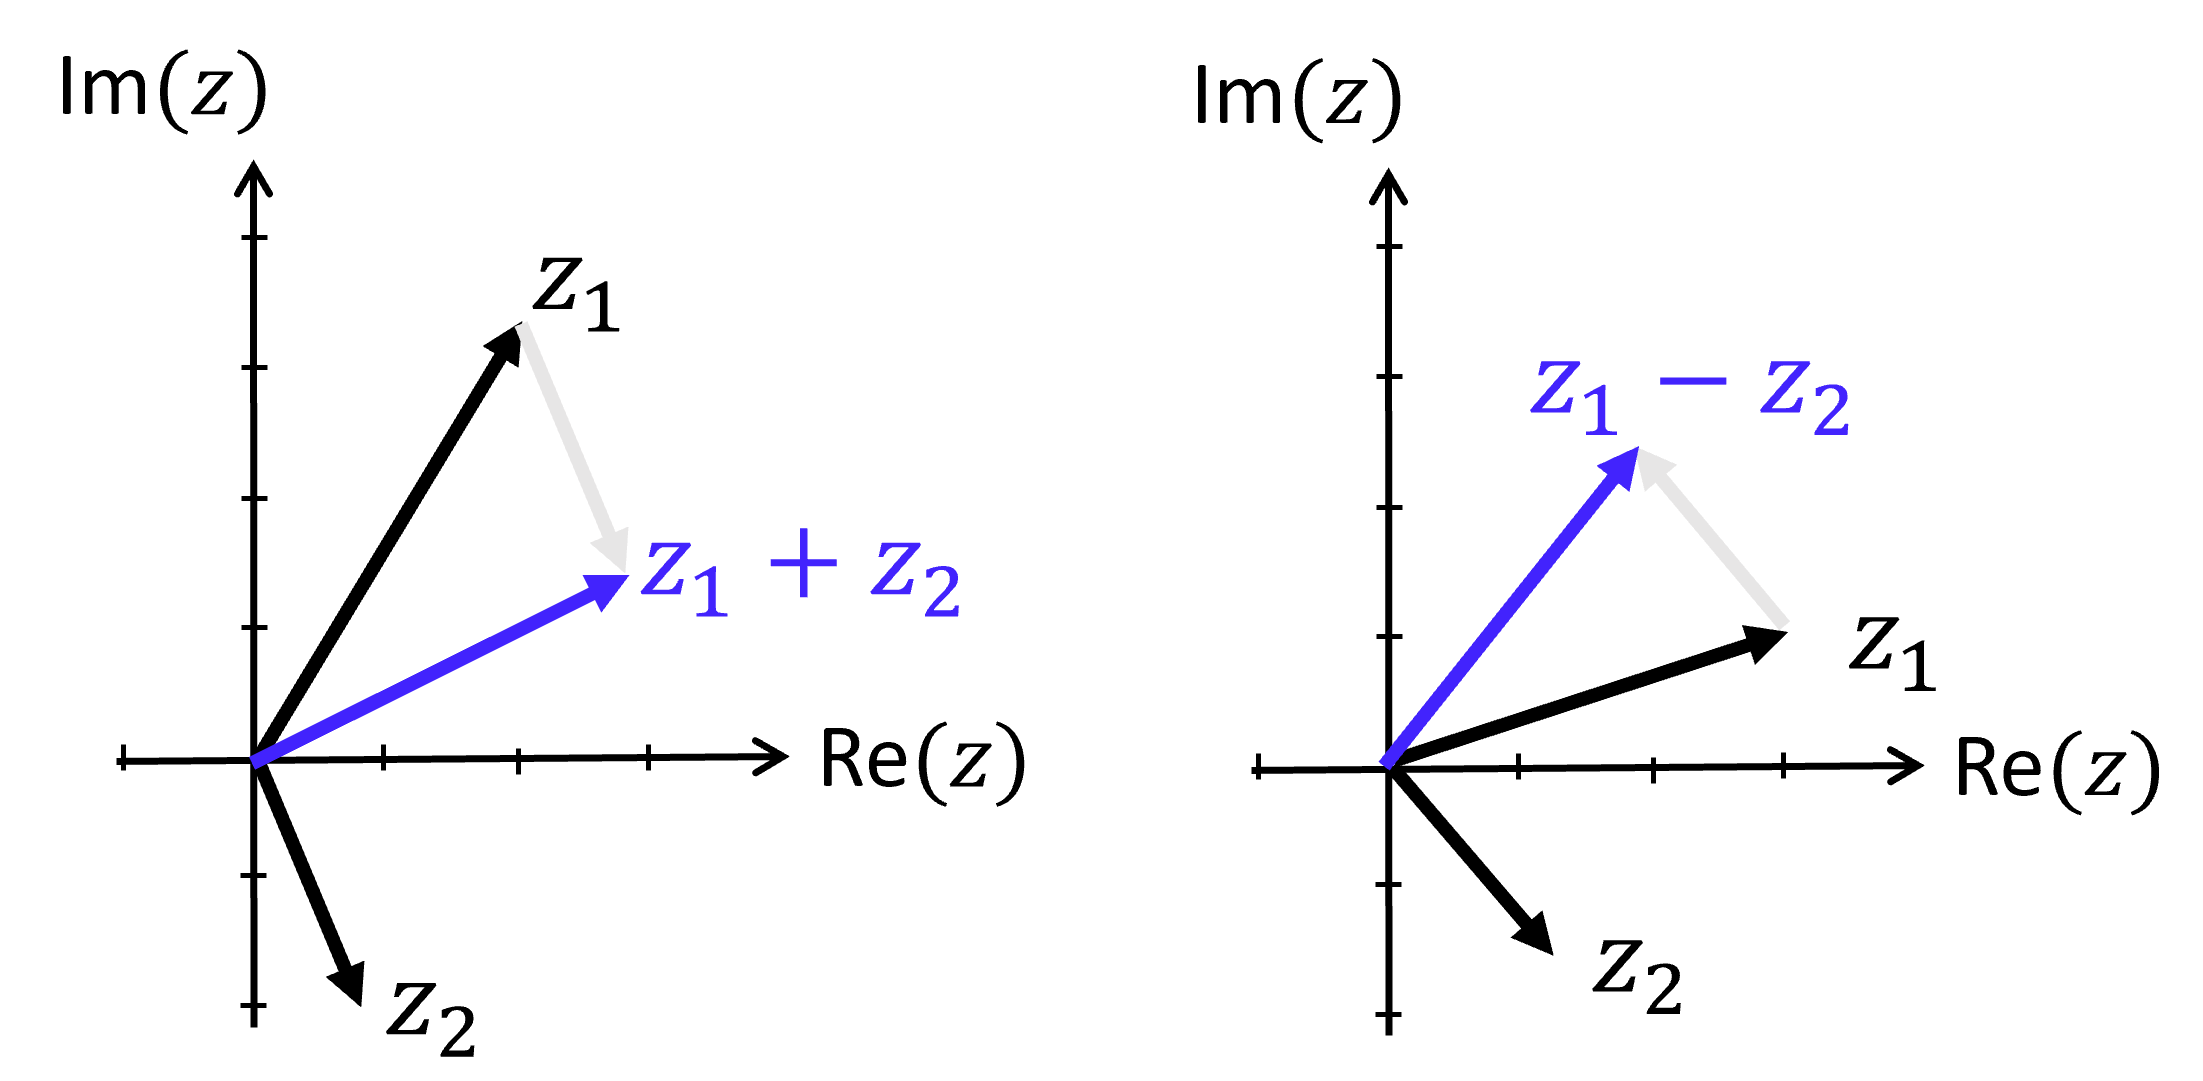
\includegraphics[width=\textwidth]{../Mathematik_1/Bilder/komplexe_zahlen_addition_subtraktion_pfeile.png}
\end{minipage}
\begin{minipage}{0.53\textwidth}

F�r
\[
	z_1=1-2\,i
\qquad\text{und}\qquad
z_2=3+4\,i
\]
gilt
\[
z_1+z_2
=
(1-2\,i)+(3+4\,i)
=
4+2\,i.
\]
Geometrisch werden die beiden zugeh�rigen Pfeile addiert.

F�r die Differenz ergibt sich
\[
z_1-z_2
=
(1-2\,i)-(3+4\,i)
=
-2-6\,i.
\]
Die Subtraktion von \(z_2\) entspricht dabei der Addition des Gegenpfeils
\(-z_2\).

\end{minipage}

\end{exabox}

\subsubsection*{Multiplikation mit \(i\): eine Drehung}

Bei der Addition ist die geometrische Interpretation unmittelbar aus den
kartesischen Koordinaten ablesbar. Bei der Multiplikation ist die Situation
weniger offensichtlich. Einen ersten Zugang liefert die Multiplikation mit
der imagin�ren Einheit \(i\).

F�r
\[
z=a+i\,b
\]
gilt
\[
i\,z
=
i(a+i\,b)
=
i\,a+i^2b
=
-b+i\,a.
\]

Der Punkt
\[
(a\,|\,b)
\]
wird durch die Multiplikation mit \(i\) also auf den Punkt
\[
(-b\,|\,a)
\]
abgebildet. Diese Abbildung entspricht geometrisch einer Drehung um
\[
\frac{\pi}{2}=90^\circ
\]
gegen den Uhrzeigersinn.

\begin{exabox}{Multiplikation mit \(i\): reine Drehung}{ }

\begin{minipage}{0.4\textwidth}
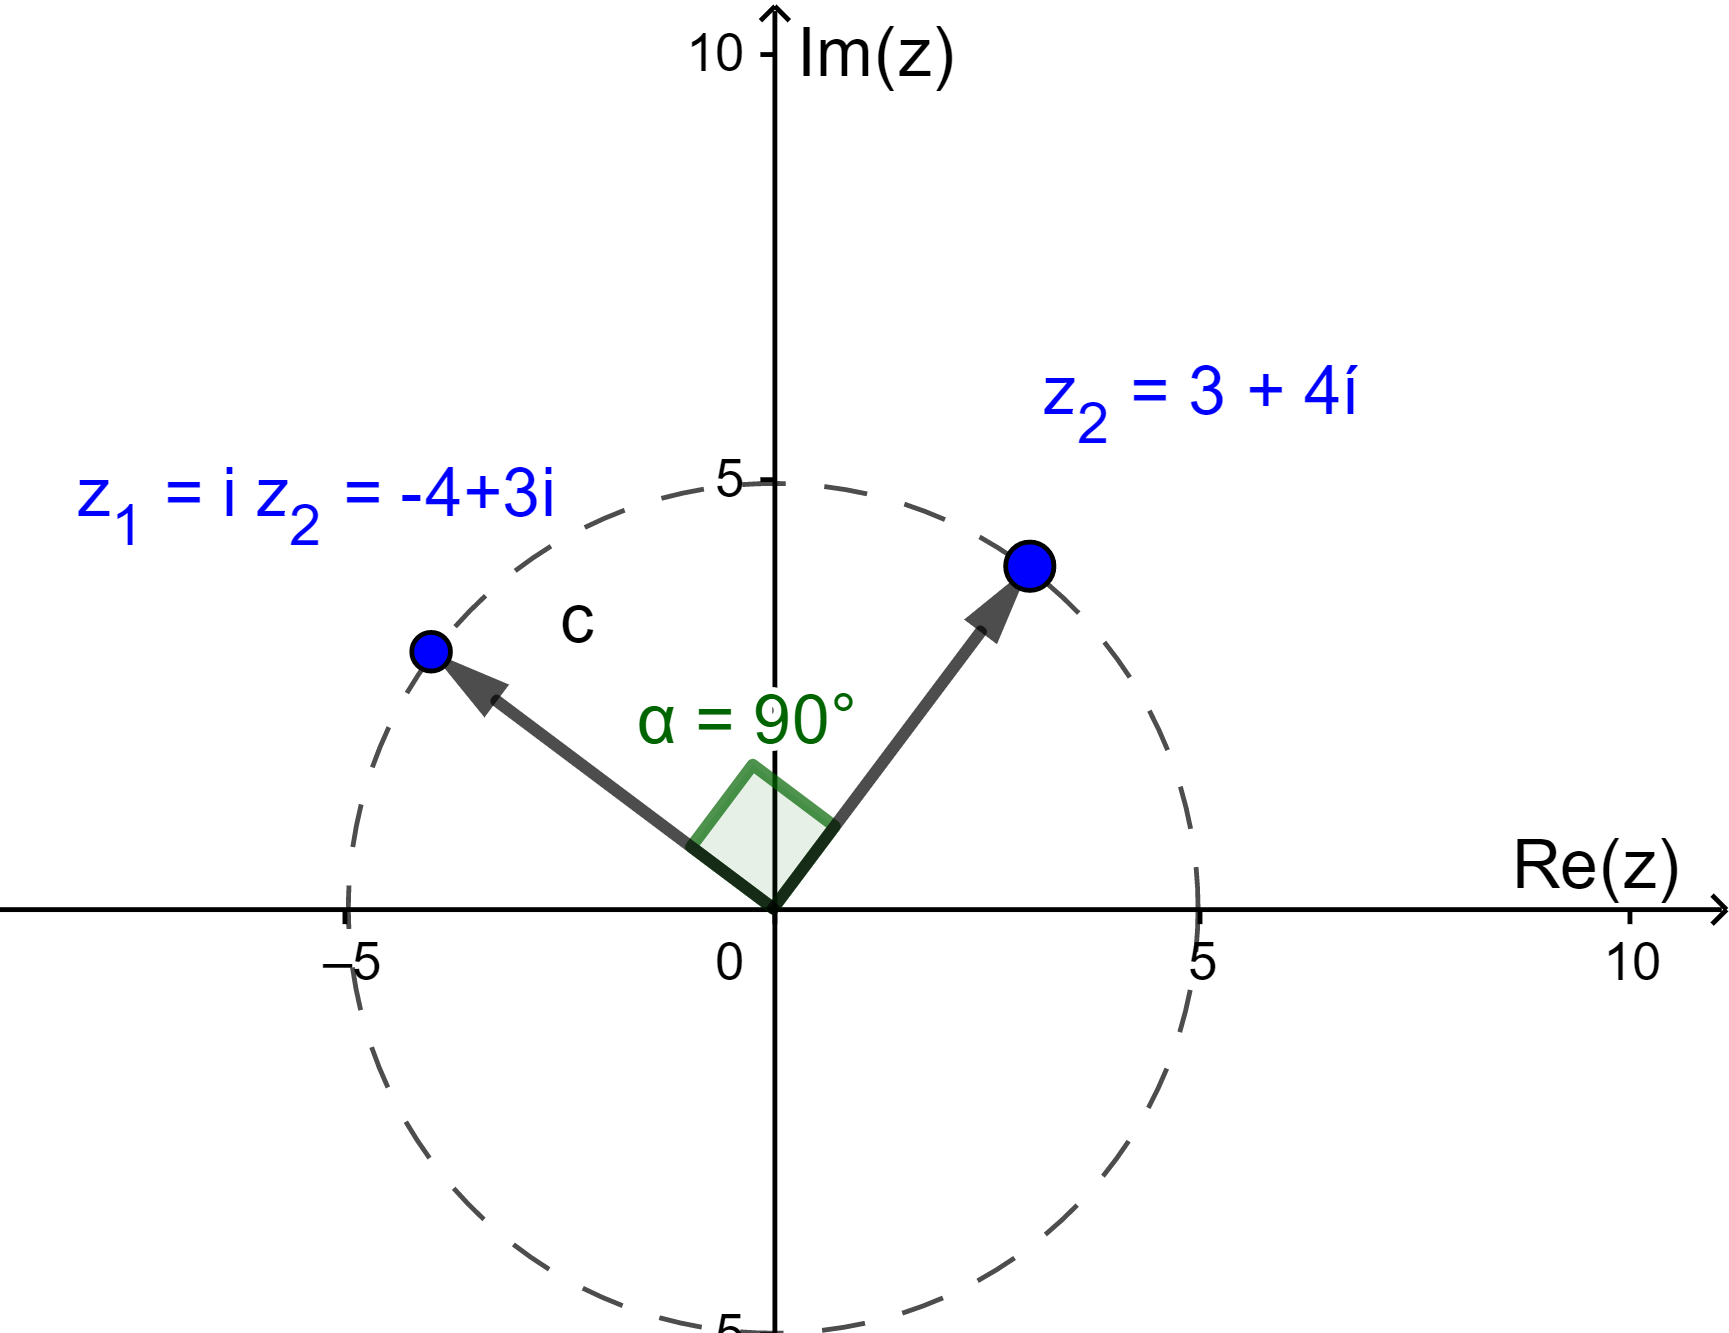
\includegraphics[width=\textwidth]{../Mathematik_1/Bilder/komplexe_zahlen_multiplikation_i_drehung.png}
\end{minipage}
\begin{minipage}{0.58\textwidth}

F�r
\[
z\;\widehat=\;(r\,|\,\varphi)
\]
bleibt bei der Multiplikation mit \(i\) die L�nge des zugeh�rigen Pfeils
unver�ndert:
\[
|i\,z|
=
\sqrt{(-b)^2+a^2}
=
\sqrt{a^2+b^2}
=
|z|
=
r.
\]

Gleichzeitig wird der Pfeil um \(90^\circ\) gegen den Uhrzeigersinn gedreht.
Sein Winkel ver�ndert sich daher von
\[
\varphi
\]
zu
\[
\varphi+\frac{\pi}{2}.
\]

Damit gilt
\[
i\,z
\;\widehat=\;
\left(
r\,\middle|\,\varphi+\frac{\pi}{2}
\right).
\]

\end{minipage}

\end{exabox}

Die Multiplikation mit \(i\) ver�ndert also nicht die L�nge einer komplexen
Zahl, sondern ausschlie�lich ihre Richtung. Sie liefert damit ein erstes
Beispiel daf�r, dass eine Multiplikation in \(\mathbb C\) geometrisch als
Drehung interpretiert werden kann.

\subsubsection*{Multiplikation: Skalierung und Drehung}

Die Multiplikation mit \(i\) zeigt bereits, dass eine Multiplikation in \(\mathbb C\) geometrisch eine Drehung bewirken kann. Bei der Multiplikation mit einer beliebigen komplexen Zahl kommt im Allgemeinen zus�tzlich eine Skalierung hinzu.

Besonders transparent wird dies in Polarkoordinaten. Es seien
\[
z_1\;\widehat=\;(r_1\,|\,\varphi_1)
\qquad\text{und}\qquad
z_2\;\widehat=\;(r_2\,|\,\varphi_2).
\]

Bei der Multiplikation werden die Betr�ge multipliziert und die Winkel
addiert.

\begin{theorembox}{Geometrische Interpretation der Multiplikation}{ }
\begin{minipage}{0.3\textwidth}
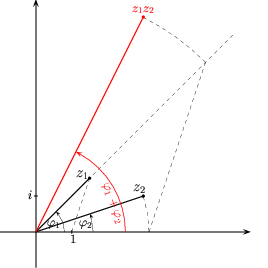
\includegraphics[width=\textwidth]{../Mathematik_1/Bilder/komplexe_zahlen_multiplikation_winkelsumme.png}
\end{minipage}
\begin{minipage}{0.7\textwidth}

F�r
\[
z_1\;\widehat=\;(r_1\,|\,\varphi_1)
\qquad\text{und}\qquad
z_2\;\widehat=\;(r_2\,|\,\varphi_2)
\]
gilt
\[
z_1\cdot z_2
\;\widehat=\;
(r_1\cdot r_2\,|\,\varphi_1+\varphi_2).
\]

Die Multiplikation komplexer Zahlen besitzt damit zwei geometrische
Wirkungen:
\begin{itemize}
    \item Die L�ngen werden multipliziert:
    \[
    |z_1\cdot z_2|=|z_1|\,|z_2|=r_1\cdot r_2.
    \]

    \item Die Winkel werden addiert:
    \[
    \arg(z_1\cdot z_2)
    =
    \varphi_1+\varphi_2
    \qquad \text{bis auf Vielfache von }2\pi.
    \]
\end{itemize}
\end{minipage}

\end{theorembox}

Eine Multiplikation mit einer komplexen Zahl kann somit als Kombination aus
\textbf{Skalierung} und \textbf{Drehung} interpretiert werden. Der Betrag des
Multiplikators bestimmt den Skalierungsfaktor, sein Argument den Drehwinkel.


\subsubsection*{Division: umgekehrte Skalierung und Drehung}

Auch die geometrische Bedeutung der Division l�sst sich aus der
Multiplikation herleiten.

Gesucht sei
\[
z_3=\frac{z_1}{z_2},
\qquad z_2\neq0.
\]
Diese Gleichung ist �quivalent zu
\[
z_2\cdot z_3=z_1.
\]

F�r die Betr�ge gilt daher
\[
r_2\cdot r_3=r_1.
\]
Da \(z_2\neq0\) und damit \(r_2>0\) ist, folgt
\[
r_3=\frac{r_1}{r_2}.
\]

F�r die Winkel gilt entsprechend
\[
\varphi_2+\varphi_3
=
\varphi_1
\qquad
\text{bis auf Vielfache von }2\pi.
\]
Damit ergibt sich
\[
\varphi_3
=
\varphi_1-\varphi_2
\qquad
\text{bis auf Vielfache von }2\pi.
\]

\begin{theorembox}{Geometrische Interpretation der Division}{ }

\begin{minipage}{0.3\textwidth}
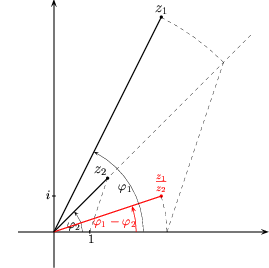
\includegraphics[width=\textwidth]{../Mathematik_1/Bilder/komplexe_zahlen_division_winkeldifferenz.png}
\end{minipage}
\begin{minipage}{0.7\textwidth}

F�r
\[
z_1\;\widehat=\;(r_1\,|\,\varphi_1),
\qquad
z_2\;\widehat=\;(r_2\,|\,\varphi_2),
\qquad
z_2\neq0,
\]
gilt
\[
\frac{z_1}{z_2}
\;\widehat=\;
\left(
\frac{r_1}{r_2}
\,\middle|\,
\varphi_1-\varphi_2
\right).
\]

Bei der Division werden somit die L�ngen dividiert und die Winkel
subtrahiert.
\end{minipage}

\end{theorembox}

\noindent\textbf{Bemerkung:}
Winkel sind nur bis auf ganzzahlige Vielfache von \(2\pi\) eindeutig
bestimmt. Bei der Addition oder Subtraktion von Argumenten kann daher ein
Winkel entstehen, der au�erhalb des gew�hlten Hauptintervalls
\[
(-\pi,\pi]
\]
liegt. Durch Addition oder Subtraktion eines geeigneten ganzzahligen
Vielfachen von \(2\pi\) kann wieder der entsprechende Hauptwert bestimmt
werden.

\medskip

Die geometrische Interpretation der Grundrechenarten l�sst sich damit
besonders kompakt zusammenfassen:
\[
\begin{array}{ccl}
\text{Addition}
&\longleftrightarrow&
\text{Pfeiladdition},\\[1mm]
\text{Multiplikation}
&\longleftrightarrow&
\text{L�ngen multiplizieren und Winkel addieren},\\[1mm]
\text{Division}
&\longleftrightarrow&
\text{L�ngen dividieren und Winkel subtrahieren}.
\end{array}
\]

Insbesondere die Multiplikation zeigt, warum die Polardarstellung f�r
komplexe Zahlen so n�tzlich ist. In kartesischer Darstellung ist eine
Multiplikation vergleichsweise aufwendig; in Polarkoordinaten werden
lediglich Betr�ge multipliziert und Winkel addiert.

Diese Beobachtung bildet den Ausgangspunkt f�r die n�chste Darstellung
komplexer Zahlen. Die Beziehung
\[
z
=
r\bigl(\cos(\varphi)+i\sin(\varphi)\bigr)
\]
wird dort mithilfe der komplexen Exponentialfunktion in eine noch kompaktere
Form �berf�hrt.

 \newpage % Komplexe Zahlen Grundlagen
\setcounter{exercise}{0} 
\ifintegriereaufgaben
\section*{Komplexe Zahlen I Aufgaben}\label{MA1-komplexe-zahlen-grundlagen-aufgaben}

	Regeln und Beispiele, die zur Bearbeitung der Aufgaben hilfreich sind, finden Sie im Skript\wennreferenzvorhanden{MA1-komplexe-zahlen-grundlagen}{ (Abschnitt \abschnittsverweis{MA1-komplexe-zahlen-grundlagen})} und, falls Sie nicht weiterkommen, schauen Sie \hyperref[MA1-komplexe-zahlen-grundlagen-loesungen]{hier}.
\else
\section{Komplexe Zahlen I Aufgaben}\label{MA1-komplexe-zahlen-grundlagen-aufgaben}

	Regeln und Beispiele, die zur Bearbeitung der Aufgaben hilfreich sind, finden Sie im Skript und, falls Sie nicht weiterkommen, schauen Sie \hyperref[MA1-komplexe-zahlen-grundlagen-loesungen]{hier}.
\fi 

\begin{exercisebox}[Rechenregeln] %Andreas
	Gegeben sinde die komplexen Zahlen $z_1: = -2 + 4i$ und $z_2:= 1-3i$.
	\begin{itemize}
		\item[(a)] Berechnen Sie $\quad i\cdot z_1 - 2 \cdot z_2, \quad z_1 \cdot z_2, \quad \displaystyle{\frac{z_1}{z_2}}, \quad \displaystyle{\frac{2z_1 z_2}{z_1^2+z_2^2}}$.
		\item[(b)] Bestimmen Sie $\quad |z_1|,\quad |z_2|,\quad |z_1\cdot z_2|$.
		\item[(c)] Bestimmen Sie $\quad \overline{z_1},\quad \overline{z_2},\quad \overline{z_1}\cdot \overline{z_2}$.
		\item[(d)] Stellen Sie die folgenden Zahlen in der kartesischen Form dar ($a,b\in\mathbb R$):
			\[ \frac{3-21i}{4-3i} + 3(i-8), \quad (2-4i)^2+\frac{|1-\sqrt{3}i|}{i}, \quad \left| \frac{a+bi}{a-bi} + \frac{a-bi}{a+bi}\right| \]
	\end{itemize}
\end{exercisebox}

\begin{exercisebox}[Ungleichungen] %Lucy
Bestimmen Sie die Punkte der Gau�schen Zahlenebene, die folgende Eigenschaften besitzen:
\begin{itemize}
	%\item $|z|=1$ (Kreislinie)
	%\item $|z|\leq 1$ (Kreisschreibe)
	%\item $|z|> 1$  %($\mathbb R^2 \setminus \{\textnormal{Kreisschreibe}\}$)
	%\item $0<\mathrm{arg}( z) < \pi/4$  %(Ecke, $\sin(\pi/4) = \cos(\pi/4)$)
	\item[(a)]$0<|z+i|<2$ %(verschobene Kreisscheibe ohne $(0,-i)$) 
			%\begin{eqnarray*}
			%	|z-z_0| < r \Rightarrow (z+i)\overline{(z+i)} = z\overline z + i(-i) = z^2+1 < 2 \Leftrightarrow z^2 < 1 \Leftrightarrow |z| <1 
			%\end{eqnarray*}
	\item[(b)] $|z-z_1| = |z-z_2|$ %(Mittelsenkrechte zwischen $z_1$ und $z_2$)
% 	\item $\mathrm{Re}\frac{1}{z} = \frac{1}{2a}, \quad a>0, a\in \mathbb R$ (verschobene Kreislinie)\par
%
%			Beachte:
%			\begin{eqnarray*}
%				\frac{1}{x+iy} = \frac{x+iy}{x^2 - y^2} = \frac{x}{x^2 + y^2} -i \frac{y}{x^2 + y^2} = \frac{x}{x^2 + y^2}  
%			\end{eqnarray*} 
%			Also:
%               \begin{eqnarray*}
%	            \mathrm{Re}\left( \frac{1}{x+iy}\right) = \frac{x}{x^2-y^2} &=& \frac{1}{2a} \\
%	            \Leftrightarrow 2ax &=& x^2 + y^2 \Leftrightarrow  x^2 - 2ax + a^2 - a^2 + y^2 = 0 \\
%	            \Leftrightarrow (x-a)^2 + y^2 &=& a^2
%                \end{eqnarray*}
	\item[(c)] \(|z^2-\overline z^2| \geq 4\)
	%\item[(d)] \( |z^2+\overline z^2| \geq 4\)
	%\item[(e)] Welche Punktmenge der Gau�'schen Zahlenebene erf�llen (c) und (d)?
	\end{itemize}
\end{exercisebox}

\begin{exercisebox}[Die imagin�re Einheit] %Lucy
	Berechnen Sie $i^{172}$ und $i^{175}$.
\end{exercisebox}

\begin{exercisebox}[Kartesische und Polarkoordinaten] %Andreas
	\begin{itemize}
		\item[(a)] Bestimmen Sie von folgenden komplexen Zahlen die Polarkoordinaten:
			\[ z_1=i,\quad z_2=\sqrt{3}-i, \quad z_3=-1-i, \quad z_4=x-\sqrt{3}x\,i\; (x>0) \]
%$z_1=\cos(\pi/2) + i\sin(\pi/2)$
%\begin{eqnarray*}
%	z_2 = 2\cdot \left( \cos\left(-\frac{\pi}{6}\right) + i \sin\left(-\frac{\pi}{6}\right)\right)
%\end{eqnarray*}
		\item[(b)] Bestimmen Sie von folgenden komplexen Zahlen die kartesische Form:
			\[ z_1 \; \widehat= \; 1\cdot e^{-i4\pi/3},\quad z_2 \; \widehat = \; \sqrt{2}a \cdot e^{-i\pi/4} \]
	  \end{itemize}
\end{exercisebox}


\begin{exercisebox}[Kartesische und Polarkoordinaten] %Lucy
	Bestimmen Sie mit Hilfe der Polarkoordinaten die kartesische Form der folgenden komplexen Zahl: \[z= \left( \frac12 + \frac{\sqrt{3}}{2}i\right)^{60}\,.\]
\end{exercisebox}

\begin{exercisebox}[Gleichungssystem] %Andreas
	L�sen Sie das folgende lineare Gleichungssystem
	\begin{eqnarray*}
		\begin{array}{r c r c l} 
			(3-4i)\cdot z_1 &+& (2-i)\cdot z_2 &=& 4-7i \\[1ex]
	(1-2i)\cdot z_1 &+& 4i\cdot z_2 &=& -11-15i 
\end{array}
\end{eqnarray*}
\end{exercisebox}


%\begin{exercisebox}[Schatzsuche]
%\end{exercisebox}

%\begin{exercisebox}[Binonialkoeffizient]
%	\begin{eqnarray*} 
%	(z_1+z_2)^n = \sum\limits_{k=0}^{n} \binom{n}{k} z_1^{n-k} z_2^k\,.
%	\end{eqnarray*}
%\end{exercisebox}

%\begin{exercisebox}[Parallelogramm]
%	In einem Parallelogramm ist die Sume der Quadrate �ber den Diagonalen gleich der Summe der Quadrate �ber allen der Seiten.
%	\begin{eqnarray*}
%		|z_1+z_2|^2 + |z_1 - z_2|^2 &=& (z_1+z_2)\overline{(z_1+z_2)} + (z_1-z_2)\overline{(z_1-z_2)} \\ 
%		&=& (z_1+z_2)\left( \overline{z_1} + \overline{z_2}\right) +   (z_1-z_2)\left( \overline{z_1} - \overline{z_2}\right)\\  
%	&=& z_1\overline{z_1} + z_1\overline{z_2} + z_2\overline{z_1} + z_2\overline{z_2} + z_1\overline{z_1} - z_2\overline{z_1} - z_1\overline{z_2} + z_2\overline{z_2} \\  
%	&=& 2 z_1\overline{z_1} + 2 z_2\overline{z_2} = 2\left( |z_1|^2 + |z_2|^2\right)\,.
%\end{eqnarray*}
%\end{exercisebox}

%\begin{exercisebox}[Kr�fteparallelogramm/ Addition von Vektoren]
%\end{exercisebox}

%\begin{exercisebox}[Zahlenbereiche]
%  Welche Aussage ist richtig? 
%  \begin{enumerate}
%	  \item $\mathbb R \subset \mathbb C$?
%	  \item $z\in \mathbb R \Rightarrow z = \overline{z}$
%  \end{enumerate}
%\end{exercisebox}
%
%\begin{exercisebox}[Rechnen mit komplexen Zahlen]
%  Welche Aussage ist richtig?
%  \begin{enumerate}
%	  \item $\overline{\overline z} = z$
%  	  \item $\frac{\overline{z_1}}{\overline{z_2}} = \overline{\frac{z_1}{z_2}}$
%  	  \item $\overline{z_1} \cdot \overline{z_2} = \overline{z_1 \cdot z_2}$
%  	  \item $\overline{z_1} + \overline{z_2} = \overline{z_1 + z_2}$
%  \end{enumerate}
%\end{exercisebox}

%\begin{exercisebox}[Komplexe Zahlen]
%	Es sei \(z\in \mathbb C\):\begin{enumerate}
%		\item Welche Punktmenge der Gau�'schen Zahlenebene wird durch die folgende Bedingung bestimmt?\[ |z^2-\overline z^2| \geq 4\]
%		\item Welche Punktmenge der Gau�'schen Zahlenebene wird durch die folgende Bedingung bestimmt?\[ |z^2+\overline z^2| \geq 4\]
%		\item Welche Punktmenge der Gau�'schen Zahlenebene erf�llt beide zuvor genannten Bedingungen?
%	\end{enumerate}
%
%	\vspace{0.3cm}
%	\noindent{\bf L�sung:} \newline
%
%\end{exercisebox}


 \newpage 
\setcounter{satz}{0} \setcounter{def}{0} \setcounter{exa}{0}  
\section{Komplexe Zahlen II: Polarform, Euler und Schwingungen}\label{MA1-komplexe-zahlen-polarform-und-euler}

\begin{table}[H]
  \centering
  \begin{tabularx}{\textwidth}{p{0.9\textwidth} p{0.1\textwidth}}
    \toprule
    \multicolumn{2}{c}{\textbf{�bersicht �ber Lernziele und Voraussetzungen}}\\
    \midrule
    \textbf{Lernziele} &\\[.5\normalbaselineskip]
    \tabitem die Polarform komplexer Zahlen zum Potenzieren und Wurzelziehen nutzen &\\
    \tabitem alle L�sungen einer Gleichung der Form \(z^n=c\) bestimmen und geometrisch interpretieren &\\
    \tabitem die Eulersche Formel erkl�ren und komplexe Zahlen in Exponentialdarstellung schreiben &\\
    \tabitem die komplexe Exponentialfunktion geometrisch interpretieren &\\
    \tabitem harmonische Schwingungen mithilfe komplexer Amplituden (Phasoren) darstellen &\\
    \tabitem harmonische Schwingungen gleicher Frequenz mithilfe komplexer Amplituden �berlagern &\\
    \tabitem Polynome �ber \(\mathbb C\) vollst�ndig in Linearfaktoren zerlegen &\\[.5\normalbaselineskip]
    \midrule
    \textbf{Voraussetzungen} &\\[.5\normalbaselineskip]
    \tabitem Betrag, Argument und Polarform komplexer Zahlen & \abschnittsverweis{MA1-komplexe-zahlen-grundlagen}\\
    \tabitem Multiplikation und Division komplexer Zahlen in geometrischer Darstellung & \abschnittsverweis{MA1-komplexe-zahlen-grundlagen}\\
    \tabitem Potenzen und Wurzeln reeller Zahlen & \abschnittsverweis{MA1-potenz-und-wurzelfunktionen}\\
    \tabitem Exponentialfunktion & \abschnittsverweis{MA1-exponential-und-logarithmusfunktionen}\\
    \tabitem trigonometrische Funktionen und harmonische Schwingungen & \abschnittsverweis{MA1-trigonometrische-funktionen}\\
    \bottomrule
  \end{tabularx}
\end{table}

\ifintegriereaufgaben
\noindent �bungsaufgaben zu diesem Abschnitt:
\hyperref[MA1-komplexe-zahlen-polarform-und-euler-aufgaben]{Aufgaben}
\vspace{0.3cm}
\hrule
\fi


% --------------------------------------------------------------------------
\subsection{Potenzen und Wurzeln in Polarform}

Im vorangegangenen Abschnitt wurden komplexe Zahlen sowohl in kartesischer
Form \(z=a+i\,b\) als auch mithilfe von Betrag und Winkel dargestellt. F�r
\(z\neq0\) gilt
\[
z=r\bigl(\cos(\varphi)+i\sin(\varphi)\bigr),
\qquad
r=|z|,
\qquad
\varphi=\arg(z).
\]

Dabei zeigte sich bereits ein wesentlicher Vorteil der Polardarstellung. F�r
zwei komplexe Zahlen
\[
z_1\;\widehat=\;(r_1\,|\,\varphi_1),
\qquad
z_2\;\widehat=\;(r_2\,|\,\varphi_2)
\]
gilt
\[
z_1z_2
\;\widehat=\;
(r_1r_2\,|\,\varphi_1+\varphi_2).
\]
Bei einer Multiplikation werden also die Betr�ge multipliziert und die Winkel
addiert.

Diese geometrische Interpretation f�hrt unmittelbar zu zwei weiteren Fragen:
Was geschieht, wenn eine komplexe Zahl mehrfach mit sich selbst multipliziert
wird? Und wie lassen sich umgekehrt alle komplexen Zahlen bestimmen, deren
\(n\)-te Potenz eine vorgegebene komplexe Zahl ergibt?

Damit f�hren Multiplikation und Polardarstellung auf nat�rliche Weise zum
\textbf{Potenzieren} und zum \textbf{Wurzelziehen} in \(\mathbb C\).


% --------------------------------------------------------------------------
\subsubsection*{Positive ganzzahlige Potenzen}

Wird eine komplexe Zahl \(z\;\widehat=\;(r\,|\,\varphi)\) mit sich selbst
multipliziert, ergibt sich
\[
z^2=z\cdot z
\;\widehat=\;
(r^2\,|\,2\varphi).
\]
Eine weitere Multiplikation mit \(z\) liefert
\(z^3\;\widehat=\;(r^3\,|\,3\varphi)\). Dieses Muster setzt sich f�r jede
positive ganzzahlige Potenz fort.

\begin{theorembox}{Potenzieren in Polarkoordinaten}{ }

F�r \(z\;\widehat=\;(r\,|\,\varphi)\) und \(n\in\mathbb N^+\) gilt
\[
z^n
\;\widehat=\;
(r^n\,|\,n\varphi).
\]

Beim Potenzieren wird der Betrag zur \(n\)-ten Potenz erhoben, w�hrend der
Winkel mit \(n\) multipliziert wird.

\end{theorembox}

\begin{exabox}{Potenzen einer komplexen Zahl}{ }

Betrachtet wird die komplexe Zahl
\[
z
\;\widehat=\;
\left(
\sqrt2\,\middle|\,\frac{\pi}{4}
\right).
\]

F�r die zweite Potenz ergibt sich
\[
\begin{aligned}
z^2
&\;\widehat=\;
\left(
(\sqrt2)^2
\,\middle|\,
2\frac{\pi}{4}
\right)\\
&=
\left(
2\,\middle|\,\frac{\pi}{2}
\right).
\end{aligned}
\]

F�r die dritte Potenz folgt entsprechend
\[
\begin{aligned}
z^3
&\;\widehat=\;
\left(
(\sqrt2)^3
\,\middle|\,
3\frac{\pi}{4}
\right)\\
&=
\left(
2\sqrt2
\,\middle|\,
\frac{3\pi}{4}
\right).
\end{aligned}
\]

Das Beispiel macht beide Wirkungen des Potenzierens sichtbar: Der Betrag
ver�ndert sich durch die Potenz \(r^n\), w�hrend sich der Winkel mit jeder
weiteren Multiplikation um \(\varphi\) vergr��ert.

\end{exabox}

Die geometrischen Wirkung des Potenzierens l�sst sich interaktiv untersuchen, beispielsweise in der GeoGebra Anwendung
\href{https://www.geogebra.org/m/jsda7yjz}{Potenzieren komplexer Zahlen}.

\subsubsection*{Negative ganzzahlige Potenzen}

F�r \(z\neq0\) sind auch negative ganzzahlige Potenzen definiert. Dabei gilt
beispielsweise \(z^{-1}=1/z\). Die Division komplexer Zahlen wurde im
vorangegangenen Abschnitt bereits geometrisch als Division der Betr�ge und
Subtraktion der Winkel interpretiert.

F�r \(z\;\widehat=\;(r\,|\,\varphi)\) folgt daher
\[
z^{-1}
\;\widehat=\;
\left(
\frac{1}{r}\,\middle|\,-\varphi
\right).
\]

Allgemeiner gilt f�r \(n\in\mathbb N^+\)
\[
z^{-n}
\;\widehat=\;
(r^{-n}\,|\,-n\varphi).
\]

\begin{exabox}{Negative Potenzen}{ }

F�r
\[
z
\;\widehat=\;
\left(
\sqrt2\,\middle|\,\frac{\pi}{4}
\right)
\]
gilt zun�chst
\[
z^0=1
\;\widehat=\;
(1\,|\,0).
\]

F�r den Kehrwert ergibt sich
\[
z^{-1}
\;\widehat=\;
\left(
\frac{1}{\sqrt2}
\,\middle|\,
-\frac{\pi}{4}
\right).
\]

Der Betrag wird beim Bilden des Kehrwerts also invertiert, w�hrend sich das
Vorzeichen des Winkels �ndert.

\end{exabox}

Positive, negative und die nullte Potenz lassen sich damit gemeinsam
beschreiben: F�r \(z\neq0\) und \(n\in\mathbb Z\) gilt
\[
z^n
\;\widehat=\;
(r^n\,|\,n\varphi).
\]


\subsubsection*{Die Umkehrfrage: Wurzeln komplexer Zahlen}

Das Potenzieren f�hrt unmittelbar auf die Umkehrfrage. Gesucht seien
beispielsweise alle komplexen Zahlen \(z\), f�r die
\[
z^3=8i
\]
gilt.

Die rechte Seite besitzt den Betrag \(8\) und den Winkel \(\pi/2\), also
\[
8i
\;\widehat=\;
\left(
8\,\middle|\,\frac{\pi}{2}
\right).
\]

F�r die gesuchte Zahl wird
\(z\;\widehat=\;(r\,|\,\varphi)\) angesetzt. Dann gilt
\[
z^3
\;\widehat=\;
(r^3\,|\,3\varphi).
\]

Ein erster Vergleich von Betrag und Winkel liefert
\[
r^3=8
\qquad\text{und}\qquad
3\varphi=\frac{\pi}{2}.
\]
Damit ergibt sich \(r=2\) und \(\varphi=\pi/6\). Eine L�sung lautet also
\[
z_0
\;\widehat=\;
\left(
2\,\middle|\,\frac{\pi}{6}
\right).
\]

Damit ist die Gleichung jedoch noch nicht vollst�ndig gel�st. Der Winkel
\(\pi/2\) beschreibt dieselbe Richtung wie jeder Winkel
\[
\frac{\pi}{2}+2\pi k,
\qquad k\in\mathbb Z.
\]
F�r die gesuchten Winkel muss daher allgemeiner
\[
3\varphi_k
=
\frac{\pi}{2}+2\pi k
\]
gelten. Somit folgt
\[
\varphi_k
=
\frac13
\left(
\frac{\pi}{2}+2\pi k
\right).
\]

F�r \(k=0,1,2\) entstehen drei verschiedene komplexe Zahlen.

\begin{exabox}{Die drei L�sungen von \(z^3=8i\)}{ }

\begin{minipage}{0.4\textwidth}
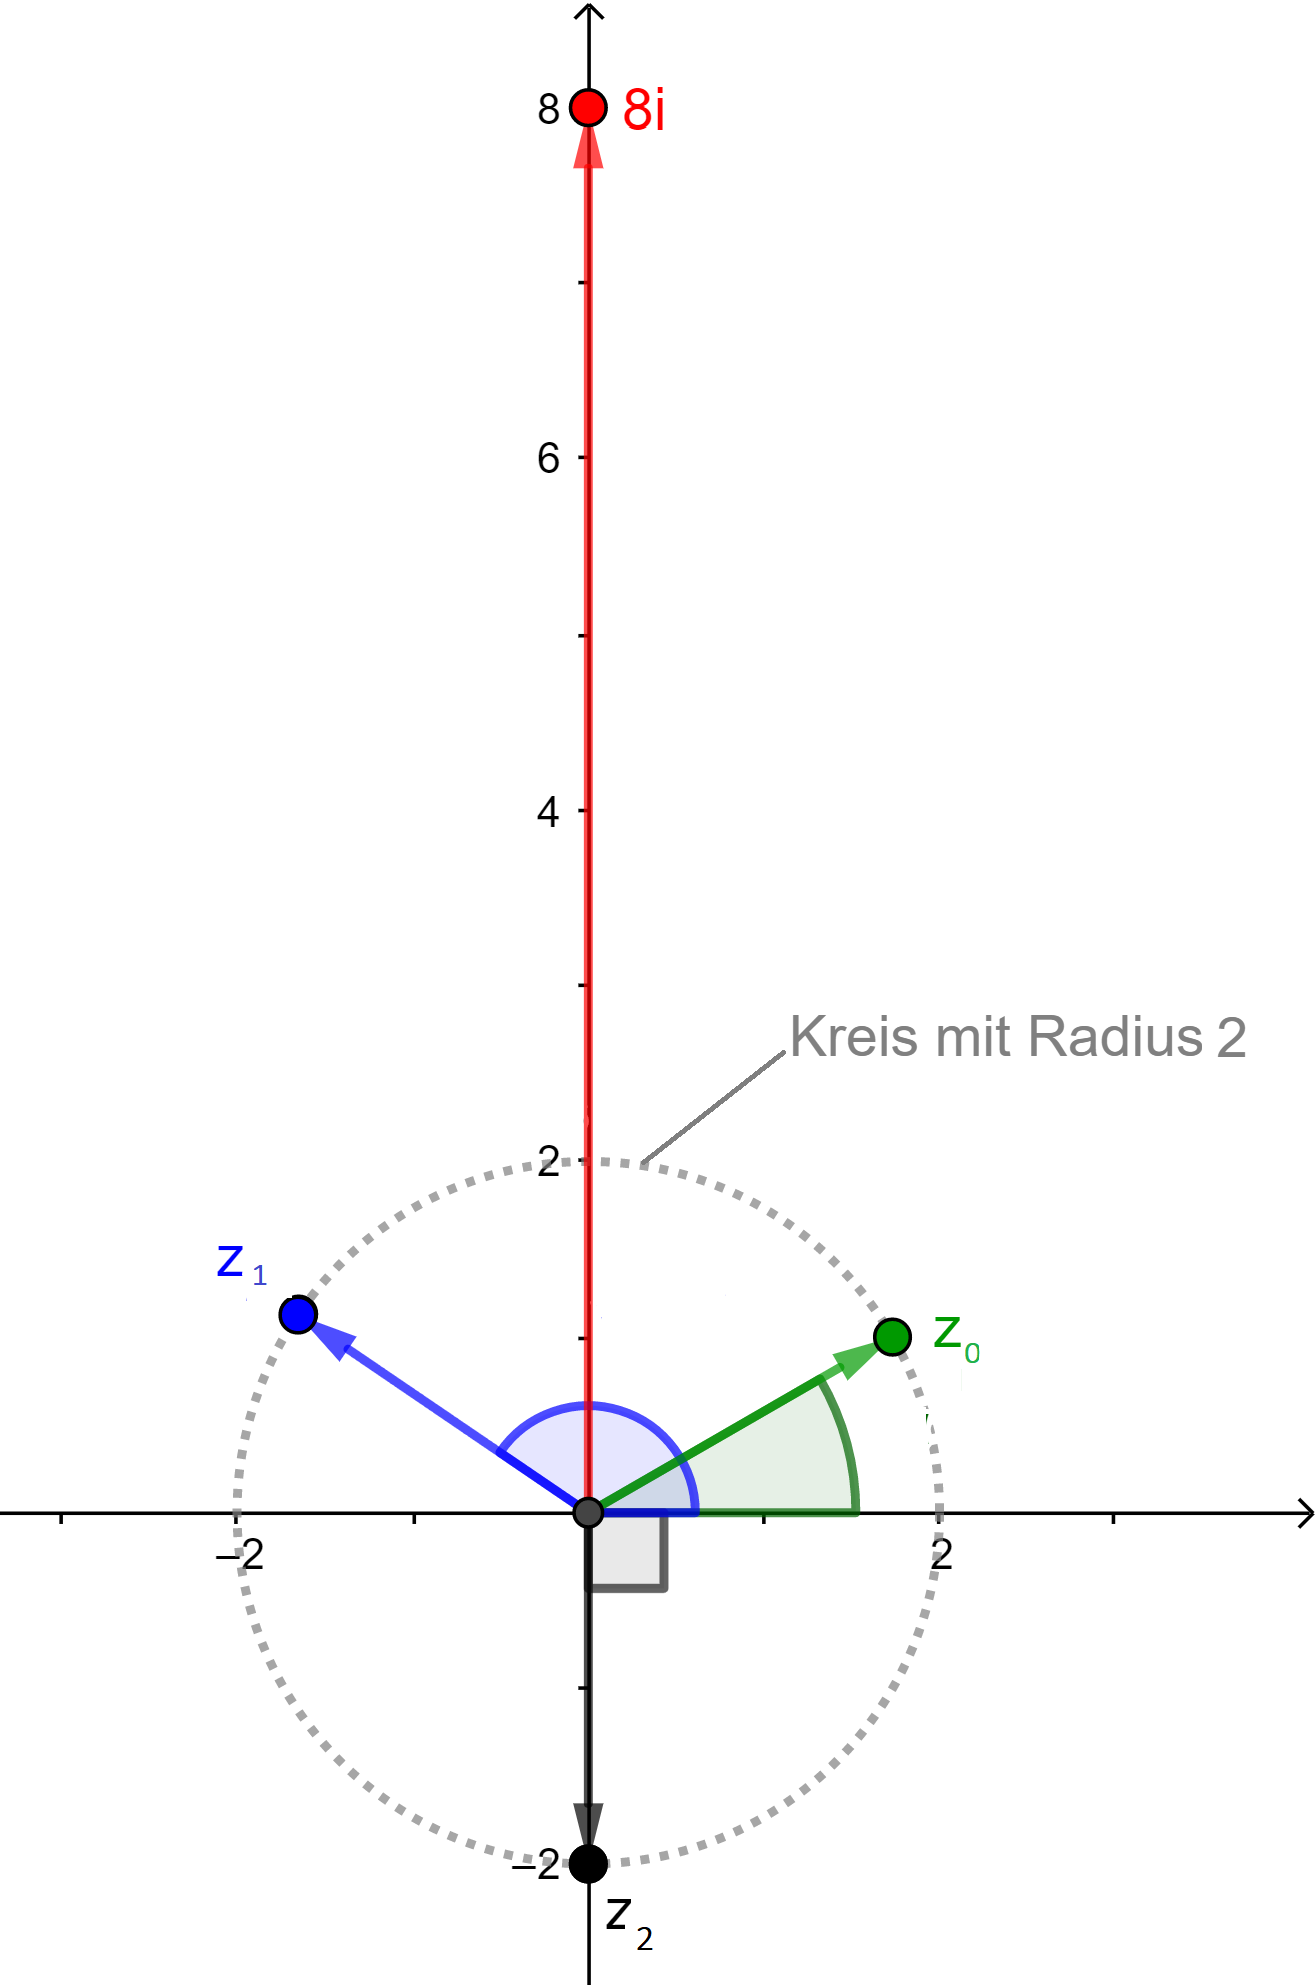
\includegraphics[width=\textwidth]{../Mathematik_1/Bilder/komplexe_zahlen_dritte_wurzeln_acht_i.png}
\end{minipage}
\begin{minipage}{0.58\textwidth}

F�r \(k=0\) gilt
\[
\varphi_0
=
\frac13\frac{\pi}{2}
=
\frac{\pi}{6},
\]
also
\[
z_0
\;\widehat=\;
\left(
2\,\middle|\,\frac{\pi}{6}
\right).
\]

F�r \(k=1\) ergibt sich
\[
\varphi_1
=
\frac13
\left(
\frac{\pi}{2}+2\pi
\right)
=
\frac{5\pi}{6},
\]
also
\[
z_1
\;\widehat=\;
\left(
2\,\middle|\,\frac{5\pi}{6}
\right).
\]

F�r \(k=2\) folgt zun�chst
\[
\varphi_2
=
\frac13
\left(
\frac{\pi}{2}+4\pi
\right)
=
\frac{3\pi}{2}.
\]
Da \(\frac{3\pi}{2}\) und \(-\frac{\pi}{2}\) dieselbe Richtung beschreiben,
kann die dritte L�sung im gew�hlten Hauptintervall als
\[
z_2
\;\widehat=\;
\left(
2\,\middle|\,-\frac{\pi}{2}
\right)
\]
geschrieben werden.

\end{minipage}

\end{exabox}

Alle drei L�sungen besitzen denselben Betrag \(2\). Sie liegen daher auf
einem Kreis mit Radius \(2\) um den Ursprung. Gleichzeitig unterscheiden
sich ihre Winkel jeweils um \(2\pi/3\). Die L�sungen sind also gleichm��ig
auf diesem Kreis verteilt.

Das Beispiel zeigt, warum das Wurzelziehen in \(\mathbb C\) anders behandelt
werden muss als in \(\mathbb R\): Die Mehrdeutigkeit der Winkel f�hrt dazu,
dass eine Gleichung der Form \(z^n=c\) im Allgemeinen mehrere verschiedene
komplexe L�sungen besitzt.


\subsubsection*{Allgemeine \(n\)-te Wurzeln}

Das Vorgehen aus dem vorangegangenen Beispiel l�sst sich auf eine beliebige
komplexe Zahl �bertragen. Gesucht seien alle L�sungen von
\[
z^n=c,
\qquad
c\in\mathbb C\setminus\{0\}.
\]

Die rechte Seite werde durch
\[
c
\;\widehat=\;
(\rho\,|\,\psi),
\qquad
\rho=|c|>0,
\]
beschrieben. F�r die gesuchte Zahl wird
\(z\;\widehat=\;(r\,|\,\varphi)\) angesetzt. Dann gilt
\[
z^n
\;\widehat=\;
(r^n\,|\,n\varphi).
\]

Da neben \(\psi\) auch alle Winkel \(\psi+2\pi k\) dieselbe komplexe Zahl
\(c\) beschreiben, m�ssen die Bedingungen
\[
r^n=\rho
\qquad\text{und}\qquad
n\varphi=\psi+2\pi k
\]
erf�llt sein.

Daraus folgen
\[
r=\sqrt[n]{\rho}
\qquad\text{und}\qquad
\varphi_k=\frac{\psi+2\pi k}{n}.
\]

\begin{theorembox}{\(n\)-te Wurzeln einer komplexen Zahl}{ }

F�r
\[
c
=
\rho\bigl(\cos(\psi)+i\sin(\psi)\bigr)
\neq0
\]
besitzt die Gleichung \(z^n=c\) genau \(n\) verschiedene L�sungen
\[
z_k
=
\sqrt[n]{\rho}
\left(
\cos\left(\frac{\psi+2\pi k}{n}\right)
+
i\sin\left(\frac{\psi+2\pi k}{n}\right)
\right),
\]
wobei
\[
k=0,1,\ldots,n-1.
\]

Alle \(n\) L�sungen besitzen denselben Betrag \(\sqrt[n]{\rho}\) und liegen
daher auf einem Kreis um den Ursprung. Die Winkel zweier aufeinanderfolgender
L�sungen unterscheiden sich um \(2\pi/n\). Die \(n\) Wurzeln sind somit
gleichm��ig auf diesem Kreis verteilt.

\end{theorembox}

Die \(n\) verschiedenen L�sungen entstehen also nicht durch verschiedene
Betr�ge, sondern durch die verschiedenen Winkel, die sich aus der
Mehrdeutigkeit des Arguments ergeben.

\noindent\textbf{Bemerkung:}
Das Symbol \(\sqrt[n]{c}\) ist bei komplexen Zahlen mit Vorsicht zu
interpretieren. W�hrend eine Gleichung wie \(z^n=c\) alle \(n\) L�sungen
beschreibt, bezeichnet ein Wurzelsymbol je nach Konvention h�ufig nur einen
ausgew�hlten Hauptwert. Bei der L�sung komplexer Gleichungen ist die
Formulierung \(z^n=c\) daher h�ufig eindeutiger.


\subsection{Von der Polarform zur komplexen Exponentialfunktion}

Die Polardarstellung hat gezeigt, dass die Multiplikation komplexer Zahlen
eine besonders einfache Wirkung auf ihre geometrischen Gr��en besitzt:
Betr�ge werden multipliziert und Winkel addiert.

Damit erinnert das Verhalten der Winkel an eine bereits bekannte Eigenschaft
der Exponential- beziehungsweise Logarithmusrechnung. Auch dort wird eine
Addition im Exponenten bei der Exponentialfunktion zu einer Multiplikation:
\[
e^{x+y}=e^x e^y.
\]

Es liegt daher nahe, nach einer Darstellung zu suchen, in der auch die
Addition von Winkeln durch die bekannten Potenzgesetze beschrieben werden
kann. Genau diese Verbindung wird durch die komplexe Exponentialfunktion
hergestellt.


\subsubsection*{Motivation auf dem Einheitskreis}

Auf dem Einheitskreis besitzt jede komplexe Zahl den Betrag \(1\) und ist
damit vollst�ndig durch ihren Winkel bestimmt. F�r einen Winkel \(\alpha\)
gilt
\[
c
=
\cos(\alpha)+i\sin(\alpha).
\]

Die folgende �berlegung motiviert, warum an dieser Stelle gerade die
Exponentialfunktion auftritt. Sie dient als anschaulicher Zugang und ersetzt
keinen vollst�ndigen analytischen Beweis.

Wird der Winkel \(\alpha\) in \(n\) kleine gleich gro�e Winkel zerlegt, so
besitzt die zugeh�rige komplexe Zahl
\[
z
\;\widehat=\;
\left(
1\,\middle|\,\frac{\alpha}{n}
\right)
\]
die Eigenschaft \(z^n=c\).

F�r gro�e \(n\) ist der Winkel \(\alpha/n\) klein. Auf dem Einheitskreis liegt
der zugeh�rige Punkt dann nahe bei \(1\). F�r kleine Winkel gilt n�herungsweise
\[
\cos\left(\frac{\alpha}{n}\right)\approx1
\qquad\text{und}\qquad
\sin\left(\frac{\alpha}{n}\right)\approx\frac{\alpha}{n}.
\]
Damit ergibt sich
\[
z
=
\cos\left(\frac{\alpha}{n}\right)
+
i\sin\left(\frac{\alpha}{n}\right)
\approx
1+i\frac{\alpha}{n}.
\]

Da \(c=z^n\) gilt, folgt n�herungsweise
\[
c
\approx
\left(
1+i\frac{\alpha}{n}
\right)^n.
\]

Dieser Ausdruck erinnert an die bekannte Grenzwertdarstellung der
Exponentialfunktion
\[
e^x
=
\lim_{n\to\infty}
\left(
1+\frac{x}{n}
\right)^n.
\]
Wird diese Struktur auf das komplexe Argument \(x=i\alpha\) erweitert, f�hrt
sie auf die Verbindung zwischen Exponentialfunktion und Einheitskreis.


\subsubsection*{Eulersche Formel}

\begin{theorembox}{Eulersche Formel}{ }

F�r jeden reellen Winkel \(\varphi\) gilt
\[
e^{i\varphi}
=
\cos(\varphi)+i\sin(\varphi).
\]

\end{theorembox}

Die Eulersche Formel verbindet drei zuvor getrennt betrachtete mathematische
Objekte: die Exponentialfunktion, die trigonometrischen Funktionen und die
Geometrie des Einheitskreises.

Da
\[
|e^{i\varphi}|=1,
\]
liegt \(e^{i\varphi}\) f�r jedes \(\varphi\in\mathbb R\) auf dem
Einheitskreis. Sein Argument ist \(\varphi\) bis auf ganzzahlige Vielfache
von \(2\pi\).

F�r den besonderen Winkel \(\varphi=\pi\) gilt
\[
e^{i\pi}
=
\cos(\pi)+i\sin(\pi)
=
-1.
\]
Damit folgt
\[
e^{i\pi}+1=0.
\]
Diese besondere Beziehung wird als \textbf{Eulersche Identit�t}
(\emph{Euler's identity}) bezeichnet.


\subsubsection*{Exponentialdarstellung komplexer Zahlen}

Eine beliebige komplexe Zahl \(z\neq0\) besitzt in Polardarstellung die Form
\[
z
=
r\bigl(\cos(\varphi)+i\sin(\varphi)\bigr).
\]
Mit der Eulerschen Formel kann der Ausdruck in der Klammer durch
\(e^{i\varphi}\) ersetzt werden. Damit ergibt sich
\[
z=r\,e^{i\varphi}.
\]

\begin{theorembox}{Exponentialdarstellung komplexer Zahlen}{ }

F�r jede komplexe Zahl \(z\neq0\) gilt
\[
z=r\,e^{i\varphi},
\]
wobei \(r=|z|>0\) und \(\varphi\) ein Argument von \(z\) ist.

Die Winkel \(\varphi+2\pi k\) mit \(k\in\mathbb Z\) beschreiben dieselbe
komplexe Zahl, denn
\[
e^{i(\varphi+2\pi k)}
=
e^{i\varphi}.
\]

\end{theorembox}

Die Exponentialdarstellung ist damit keine neue geometrische Darstellung, sondern eine besonders kompakte Schreibweise der bereits bekannten Polardarstellung.

Ihr Vorteil zeigt sich unmittelbar beim Rechnen. F�r \(z_1=r_1e^{i\varphi_1}\) und \(z_2=r_2e^{i\varphi_2}\) gilt
\[
z_1z_2
=
r_1r_2e^{i(\varphi_1+\varphi_2)}
\]
und f�r \(z_2\neq0\)
\[
\frac{z_1}{z_2}
=
\frac{r_1}{r_2}
e^{i(\varphi_1-\varphi_2)}.
\]

Auch die zuvor geometrisch entwickelte Potenzregel erh�lt nun eine besonders kurze algebraische Form:
\[
\left(re^{i\varphi}\right)^n
=
r^n e^{in\varphi}.
\]

Die Exponentialdarstellung liefert damit dieselben Regeln, die zuvor aus der Geometrie der komplexen Zahlen gewonnen wurden. Sie fasst diese Regeln jedoch in der bekannten Algebra der Exponentialfunktion zusammen.


\subsubsection*{Sinus und Kosinus mithilfe der Exponentialfunktion}

Die Eulersche Formel kann auch verwendet werden, um Sinus und Kosinus durch komplexe Exponentialfunktionen darzustellen. Neben
\[
e^{i\varphi}
=
\cos(\varphi)+i\sin(\varphi)
\]
gilt wegen der Symmetrieeigenschaften von Sinus und Kosinus
\[
e^{-i\varphi}
=
\cos(\varphi)-i\sin(\varphi).
\]

Durch Addition beider Gleichungen folgt
\[
e^{i\varphi}+e^{-i\varphi}
=
2\cos(\varphi),
\]
also
\[
\cos(\varphi)
=
\frac12
\left(
e^{i\varphi}+e^{-i\varphi}
\right).
\]

Durch Subtraktion ergibt sich
\[
e^{i\varphi}-e^{-i\varphi}
=
2i\sin(\varphi)
\]
und damit
\[
\sin(\varphi)
=
\frac{1}{2i}
\left(
e^{i\varphi}-e^{-i\varphi}
\right).
\]

Diese Darstellungen spielen insbesondere bei der Untersuchung von
Schwingungen eine wichtige Rolle.

\subsection{Die komplexe Exponentialfunktion}

Die Eulersche Formel beschreibt zun�chst die Exponentialfunktion f�r rein
imagin�re Zahlen. Sie erm�glicht zugleich, die Exponentialfunktion auf
beliebige komplexe Zahlen zu erweitern.

F�r
\[
z=a+i\,b,
\qquad
a,b\in\mathbb R,
\]
gilt
\[
e^z
=
e^{a+ib}
=
e^a e^{ib}.
\]
Mit der Eulerschen Formel folgt
\[
e^z
=
e^a\bigl(\cos(b)+i\sin(b)\bigr).
\]

\begin{defbox}{Komplexe Exponentialfunktion}{ }

Die \textbf{komplexe Exponentialfunktion}
(\emph{complex exponential function}) ist die Abbildung
\[
\exp:\mathbb C\to\mathbb C,
\qquad
z\mapsto e^z,
\]
mit
\[
e^{a+ib}
=
e^a\bigl(\cos(b)+i\sin(b)\bigr).
\]

\end{defbox}

Diese Darstellung zeigt, dass Real- und Imagin�rteil des Exponenten
unterschiedliche geometrische Wirkungen besitzen. F�r \(z=a+i\,b\) bestimmt
der Realteil \(a\) �ber den Faktor \(e^a\) den Betrag, w�hrend der
Imagin�rteil \(b\) den Winkel bestimmt.

Insbesondere gilt
\[
|e^{a+ib}|=e^a.
\]
Eine Ver�nderung des Realteils ver�ndert somit den Betrag, w�hrend eine
Ver�nderung des Imagin�rteils eine Drehung in der komplexen Ebene bewirkt.


% --------------------------------------------------------------------------
\subsubsection*{Komplexe Exponentialfunktionen einer reellen Variablen}

F�r die Beschreibung zeitabh�ngiger Vorg�nge wird nun die komplexe
Exponentialfunktion mit einer reellen Variablen \(t\) verbunden. Dazu sei
\[
\lambda=\sigma+i\omega
\]
eine feste komplexe Zahl. Betrachtet wird die Funktion
\[
f:\mathbb R\to\mathbb C,
\qquad
t\mapsto e^{\lambda t}.
\]

Da
\[
\lambda t
=
(\sigma+i\omega)t
=
\sigma t+i\omega t,
\]
ergibt sich
\[
\begin{aligned}
e^{\lambda t}
&=
e^{(\sigma+i\omega)t}\\
&=
e^{\sigma t}e^{i\omega t}\\
&=
e^{\sigma t}
\bigl(\cos(\omega t)+i\sin(\omega t)\bigr).
\end{aligned}
\]

Diese Darstellung verbindet zwei geometrisch unterschiedliche Vorg�nge.
Der Faktor \(e^{\sigma t}\) bestimmt die L�nge des zugeh�rigen Zeigers,
w�hrend \(e^{i\omega t}\) seine Drehung beschreibt.

F�r den Betrag gilt
\[
|e^{\lambda t}|=e^{\sigma t}.
\]
Damit h�ngt die zeitliche Entwicklung der Zeigerl�nge vom Vorzeichen von
\(\sigma\) ab. F�r \(\sigma<0\) nimmt der Betrag exponentiell ab, f�r
\(\sigma>0\) w�chst er exponentiell. Im Fall \(\sigma=0\) bleibt der Betrag
konstant.

Der Winkel ver�ndert sich gleichzeitig mit \(\omega t\). Der Parameter
\(\omega\) bestimmt damit die Winkelgeschwindigkeit der Drehung.

Die Funktion
\[
t\mapsto e^{(\sigma+i\omega)t}
\]
verbindet somit exponentielles Wachstum beziehungsweise exponentielle
D�mpfung mit einer gleichf�rmigen Drehung in der komplexen Ebene.


% --------------------------------------------------------------------------
\subsubsection*{Der Spezialfall \(e^{i\omega t}\): rotierender Zeiger}

F�r \(\sigma=0\) vereinfacht sich die komplexe Exponentialfunktion zu
\[
e^{i\omega t}
=
\cos(\omega t)+i\sin(\omega t).
\]

Da
\[
|e^{i\omega t}|=1,
\]
bleibt die L�nge des zugeh�rigen Zeigers konstant. Mit wachsendem \(t\)
ver�ndert sich ausschlie�lich sein Winkel. Die Spitze des Zeigers bewegt
sich daher auf dem Einheitskreis.

\begin{exabox}{Rotierender Zeiger und harmonische Schwingung}{ }

\begin{minipage}{0.4\textwidth}
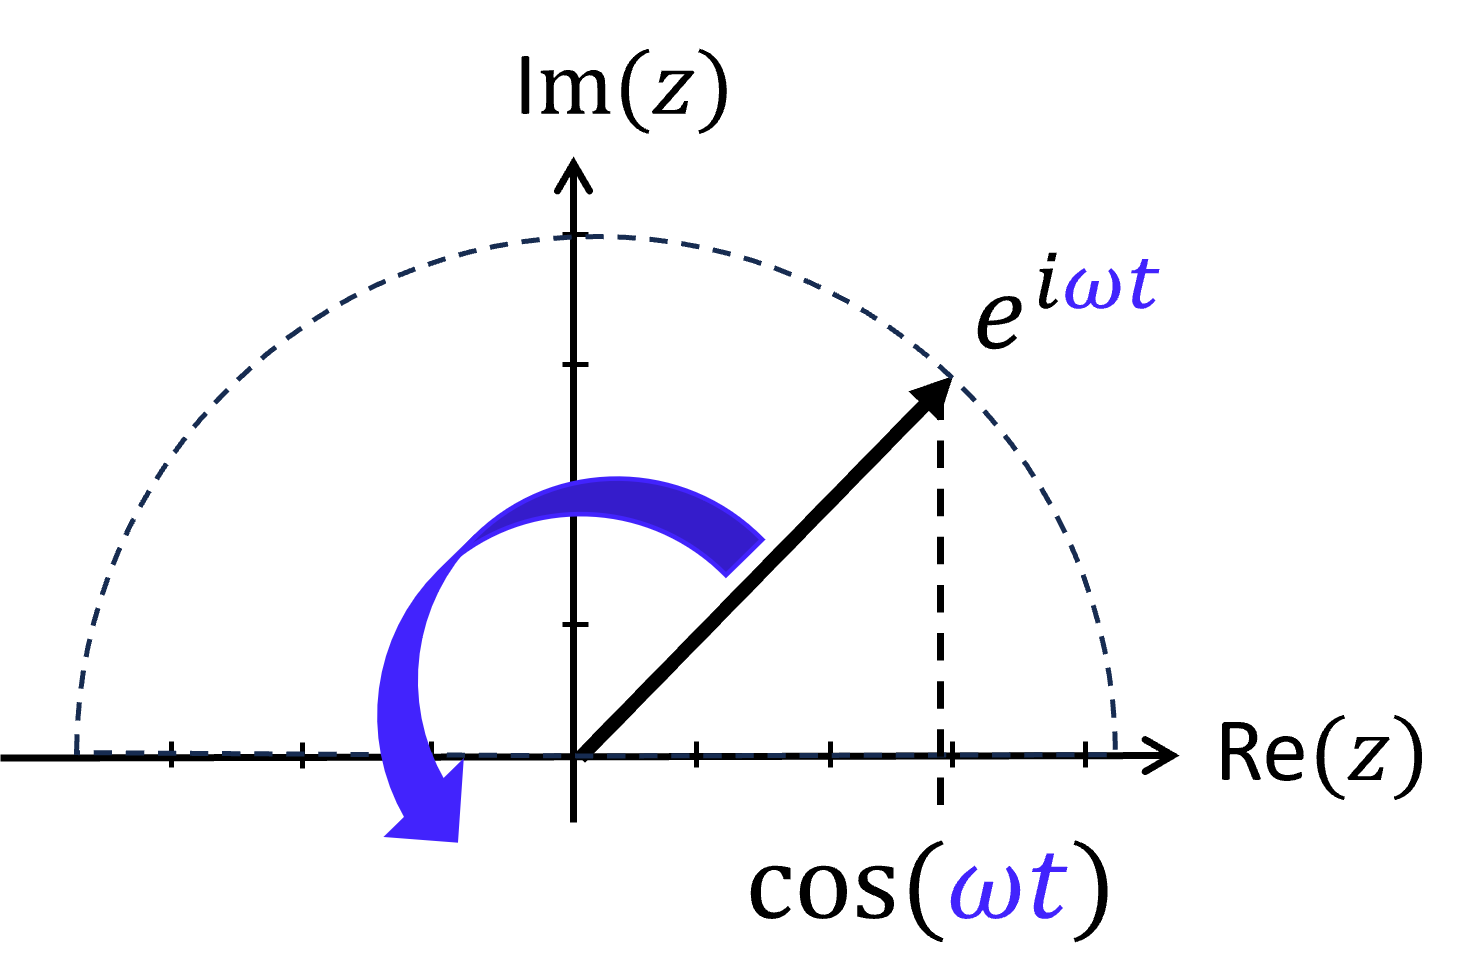
\includegraphics[width=\textwidth]{../Mathematik_1/Bilder/komplexe_zahlen_rotierender_zeiger.png}
\end{minipage}
\begin{minipage}{0.58\textwidth}

Der komplexe Ausdruck
\[
e^{i\omega t}
\]
beschreibt einen Zeiger, der sich mit der Winkelgeschwindigkeit \(\omega\)
auf dem Einheitskreis dreht.

Sein Realteil ist
\[
\mathrm{Re}\left(e^{i\omega t}\right)
=
\cos(\omega t),
\]
sein Imagin�rteil ist
\[
\mathrm{Im}\left(e^{i\omega t}\right)
=
\sin(\omega t).
\]

Die Projektion des rotierenden Zeigers auf die reelle Achse ergibt somit eine
Kosinusschwingung, die Projektion auf die imagin�re Achse eine
Sinusschwingung.

\end{minipage}

\end{exabox}

Damit erh�lt die zuvor untersuchte harmonische Schwingung eine geometrische
Interpretation: Sinus und Kosinus k�nnen als Projektionen einer
gleichf�rmigen Kreisbewegung aufgefasst werden.

Genau diese Verbindung bildet die Grundlage daf�r, harmonische Schwingungen
mithilfe komplexer Zahlen besonders kompakt zu beschreiben.

%\subsection{Die komplexe Exponentialfunktion}

%Die Eulersche Formel beschreibt zun�chst die Exponentialfunktion f�r rein
%imagin�re Argumente \(i\varphi\). Allgemeiner kann die Exponentialfunktion
%auch f�r beliebige komplexe Argumente betrachtet werden.
%
%F�r
%\[
%z=a+i\,b,
%\qquad
%a,b\in\mathbb R,
%\]
%gilt
%\[
%e^z
%=
%e^{a+ib}
%=
%e^a e^{ib}.
%\]
%Mit der Eulerschen Formel folgt
%\[
%e^z
%=
%e^a
%\bigl(
%\cos(b)+i\sin(b)
%\bigr).
%\]
%
%\begin{defbox}{Komplexe Exponentialfunktion}{ }
%
%Die \textbf{komplexe Exponentialfunktion}
%(\emph{complex exponential function}) ist die Abbildung
%\[
%\exp:\mathbb C\to\mathbb C,
%\qquad
%z\mapsto e^z,
%\]
%mit
%\[
%e^{a+ib}
%=
%e^a
%\bigl(
%\cos(b)+i\sin(b)
%\bigr).
%\]
%
%\end{defbox}
%
%Die Darstellung zeigt unmittelbar die unterschiedliche Wirkung von Real- und
%Imagin�rteil des Arguments. Der Realteil \(a\) bestimmt �ber den Faktor
%\(e^a\) den Betrag, w�hrend der Imagin�rteil \(b\) den Winkel bestimmt.
%
%Damit gilt
%\[
%|e^{a+ib}|=e^a.
%\]
%Der Imagin�rteil des Exponenten ver�ndert also nicht den Betrag, sondern nur
%die Richtung in der komplexen Ebene.
%
%
%\subsubsection*{Komplexe Exponentialfunktionen einer reellen Variablen}
%
%F�r dynamische Vorg�nge ist insbesondere eine komplexe Zahl der Form
%\[
%\lambda=\sigma+i\omega
%\]
%von Bedeutung. Wird sie mit einer reellen Variablen \(t\) multipliziert,
%entsteht die Funktion
%\[
%t\mapsto e^{\lambda t}
%=
%e^{(\sigma+i\omega)t}.
%\]
%
%Durch Zerlegen des Exponenten ergibt sich
%\[
%\begin{aligned}
%e^{(\sigma+i\omega)t}
%&=
%e^{\sigma t}e^{i\omega t}\\
%&=
%e^{\sigma t}
%\bigl(
%\cos(\omega t)+i\sin(\omega t)
%\bigr).
%\end{aligned}
%\]
%
%Damit werden zwei unterschiedliche Vorg�nge in einem einzigen Ausdruck
%verbunden:
%
%\begin{itemize}
%    \item Der Faktor \(e^{\sigma t}\) bestimmt die zeitliche Ver�nderung des
%    Betrags.
%
%    \item Der Faktor \(e^{i\omega t}\) beschreibt eine Rotation mit der
%    Winkelgeschwindigkeit \(\omega\).
%\end{itemize}
%
%F�r \(t\to+\infty\) h�ngt das Verhalten des Betrags vom Vorzeichen von
%\(\sigma\) ab. Ist \(\sigma<0\), so gilt \(e^{\sigma t}\to0\); die Bewegung
%wird exponentiell ged�mpft. F�r \(\sigma>0\) w�chst der Betrag exponentiell.
%Im Fall \(\sigma=0\) bleibt der Betrag konstant und es entsteht eine reine
%Rotation auf einem Kreis.
%
%
%\subsubsection*{Rotierender Zeiger und harmonische Schwingung}
%
%Besonders wichtig ist der Fall \(\sigma=0\). Dann gilt
%\[
%e^{i\omega t}
%=
%\cos(\omega t)+i\sin(\omega t).
%\]
%
%Die komplexe Zahl \(e^{i\omega t}\) besitzt zu jedem Zeitpunkt den Betrag
%\(1\). Mit wachsendem \(t\) ver�ndert sich lediglich ihr Winkel. Sie kann
%daher als Zeiger interpretiert werden, der sich auf dem Einheitskreis dreht.
%
%\begin{exabox}{Rotierender Zeiger und harmonische Schwingung}{ }
%
%\begin{minipage}{0.4\textwidth}
%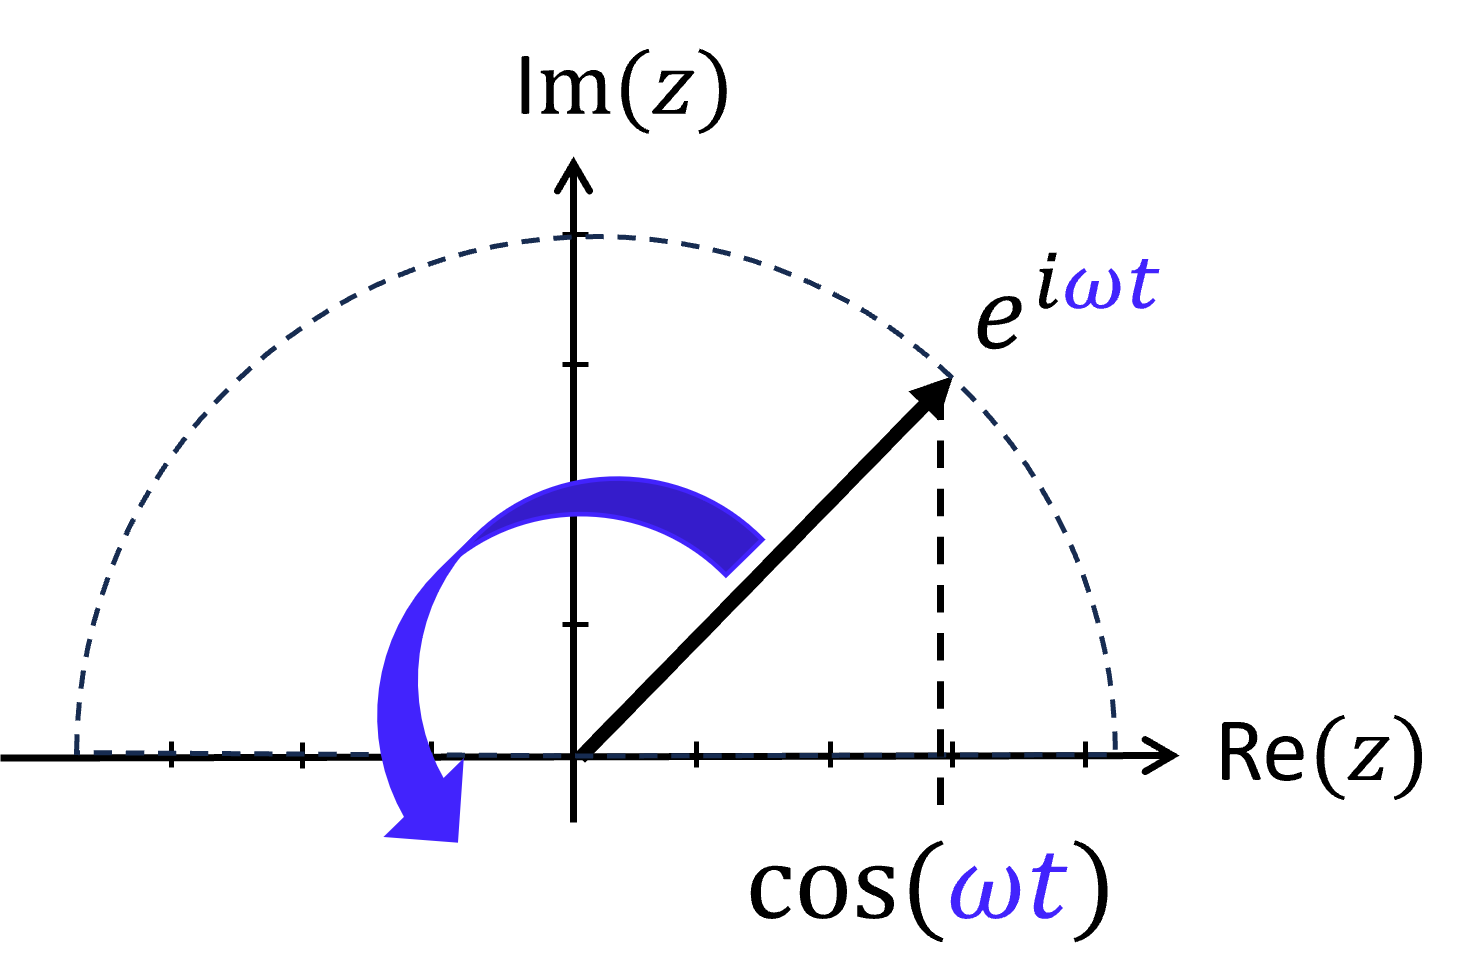
\includegraphics[width=\textwidth]{../Mathematik_1/Bilder/komplexe_zahlen_rotierender_zeiger.png}
%\end{minipage}
%\begin{minipage}{0.58\textwidth}
%
%Der komplexe Ausdruck
%\[
%e^{i\omega t}
%\]
%beschreibt einen Zeiger, der sich mit der Winkelgeschwindigkeit \(\omega\)
%auf dem Einheitskreis dreht.
%
%Sein Realteil ist
%\[
%\mathrm{Re}\left(e^{i\omega t}\right)
%=
%\cos(\omega t),
%\]
%sein Imagin�rteil
%\[
%\mathrm{Im}\left(e^{i\omega t}\right)
%=
%\sin(\omega t).
%\]
%
%Die Projektion des rotierenden Zeigers auf die reelle Achse ergibt somit eine
%Kosinusschwingung, die Projektion auf die imagin�re Achse eine
%Sinusschwingung.
%
%\end{minipage}
%
%\end{exabox}
%
%Damit erh�lt die im Kapitel �ber Funktionen untersuchte harmonische Schwingung
%eine neue geometrische Interpretation: Eine Sinus- oder Kosinusschwingung
%kann als Projektion einer gleichf�rmigen Kreisbewegung aufgefasst werden.
%
%Die komplexe Exponentialfunktion verbindet somit Rotation in der komplexen
%Ebene und harmonische Schwingung auf der reellen Achse.


%\noindent\textbf{Ausblick:}
%Die Funktionen
%\[
%t\mapsto e^{(\sigma+i\omega)t}
%\]
%verbinden exponentielles Wachstum beziehungsweise exponentielle D�mpfung mit
%einer Rotation. Dadurch k�nnen Wachstum, D�mpfung und Schwingung in einem
%einzigen mathematischen Ausdruck beschrieben werden.
%
%Diese Struktur tritt insbesondere bei der L�sung linearer
%Differentialgleichungen auf und bildet sp�ter auch eine Grundlage der
%Fourier-Analyse und der Laplace-Transformation.


\subsection{Harmonische Schwingungen und komplexe Amplituden}

Im Kapitel �ber Funktionen wurden harmonische Schwingungen in der Form
\[
s(t)
=
A\sin(\omega t+\alpha)
\]
beschrieben. Dabei bestimmt \(A\) die Amplitude, \(\omega\) die
Kreisfrequenz und \(\alpha\) die Phase.

Mithilfe der Eulerschen Formel kann dieselbe Schwingung durch eine komplexe
Exponentialfunktion dargestellt werden. Es gilt
\[
\begin{aligned}
s(t)
&=
A\sin(\omega t+\alpha)\\
&=
\mathrm{Im}
\left(
A e^{i(\omega t+\alpha)}
\right)\\
&=
\mathrm{Im}
\left(
A e^{i\alpha}e^{i\omega t}
\right).
\end{aligned}
\]

Dabei enth�lt der Faktor \(e^{i\omega t}\) die zeitabh�ngige Rotation. Die
beiden Parameter Amplitude \(A\) und Phase \(\alpha\) k�nnen dagegen in der
zeitunabh�ngigen komplexen Zahl
\[
\underline A
:=
A e^{i\alpha}
\]
zusammengefasst werden.

\begin{defbox}{Komplexe Amplitude}{ }

Die komplexe Zahl
\[
\underline A
=
A e^{i\alpha}
\]
hei�t \textbf{komplexe Amplitude} beziehungsweise \textbf{Phasor}
(\emph{phasor}).

Ihr Betrag ist die Amplitude der Schwingung,
\[
|\underline A|=A,
\]
und ihr Argument beschreibt die Phase,
\[
\arg(\underline A)=\alpha
\]
bis auf ganzzahlige Vielfache von \(2\pi\).

Die zugeh�rige Sinusschwingung kann damit in der Form
\[
s(t)
=
\mathrm{Im}
\left(
\underline A e^{i\omega t}
\right)
\]
geschrieben werden.

\end{defbox}

Diese Darstellung trennt zwei unterschiedliche Informationen voneinander:
Die gemeinsame zeitliche Rotation steckt in \(e^{i\omega t}\), w�hrend
Amplitude und Phase vollst�ndig durch die komplexe Zahl \(\underline A\)
beschrieben werden.

Gerade bei der �berlagerung mehrerer Schwingungen gleicher Frequenz f�hrt
diese Trennung zu einer erheblichen Vereinfachung.


% --------------------------------------------------------------------------
\subsubsection*{�berlagerung harmonischer Schwingungen gleicher Frequenz}

Es seien zwei harmonische Schwingungen mit derselben Kreisfrequenz
\(\omega\) gegeben. Ihre komplexen Darstellungen lauten
\[
\underline s_1(t)
=
\underline A_1e^{i\omega t}
\qquad\text{und}\qquad
\underline s_2(t)
=
\underline A_2e^{i\omega t}.
\]

Bei der Addition kann der gemeinsame zeitabh�ngige Faktor ausgeklammert
werden:
\[
\begin{aligned}
\underline s(t)
&=
\underline s_1(t)+\underline s_2(t)\\
&=
\underline A_1e^{i\omega t}
+
\underline A_2e^{i\omega t}\\
&=
(\underline A_1+\underline A_2)e^{i\omega t}.
\end{aligned}
\]

Die resultierende komplexe Amplitude ist daher einfach
\[
\underline A
=
\underline A_1+\underline A_2.
\]

\begin{theorembox}{�berlagerung gleicher Frequenz}{ }

F�r zwei komplex dargestellte harmonische Schwingungen
\[
\underline s_1(t)
=
\underline A_1e^{i\omega t},
\qquad
\underline s_2(t)
=
\underline A_2e^{i\omega t}
\]
gilt
\[
\underline s_1(t)+\underline s_2(t)
=
(\underline A_1+\underline A_2)e^{i\omega t}.
\]

Die resultierende komplexe Amplitude ist
\[
\underline A
=
\underline A_1+\underline A_2.
\]
Damit ergeben sich die Amplitude und die Phase der resultierenden Schwingung
aus
\[
A=|\underline A|
\qquad\text{und}\qquad
\alpha=\arg(\underline A).
\]

\end{theorembox}

Die �berlagerung harmonischer Schwingungen gleicher Frequenz wird damit auf
die Addition zweier komplexer Zahlen zur�ckgef�hrt. Geometrisch entspricht
dies der bereits bekannten Pfeiladdition in der Gau�schen Zahlenebene.

\begin{exabox}{Addition komplexer Amplituden}{ }

\begin{minipage}{0.4\textwidth}
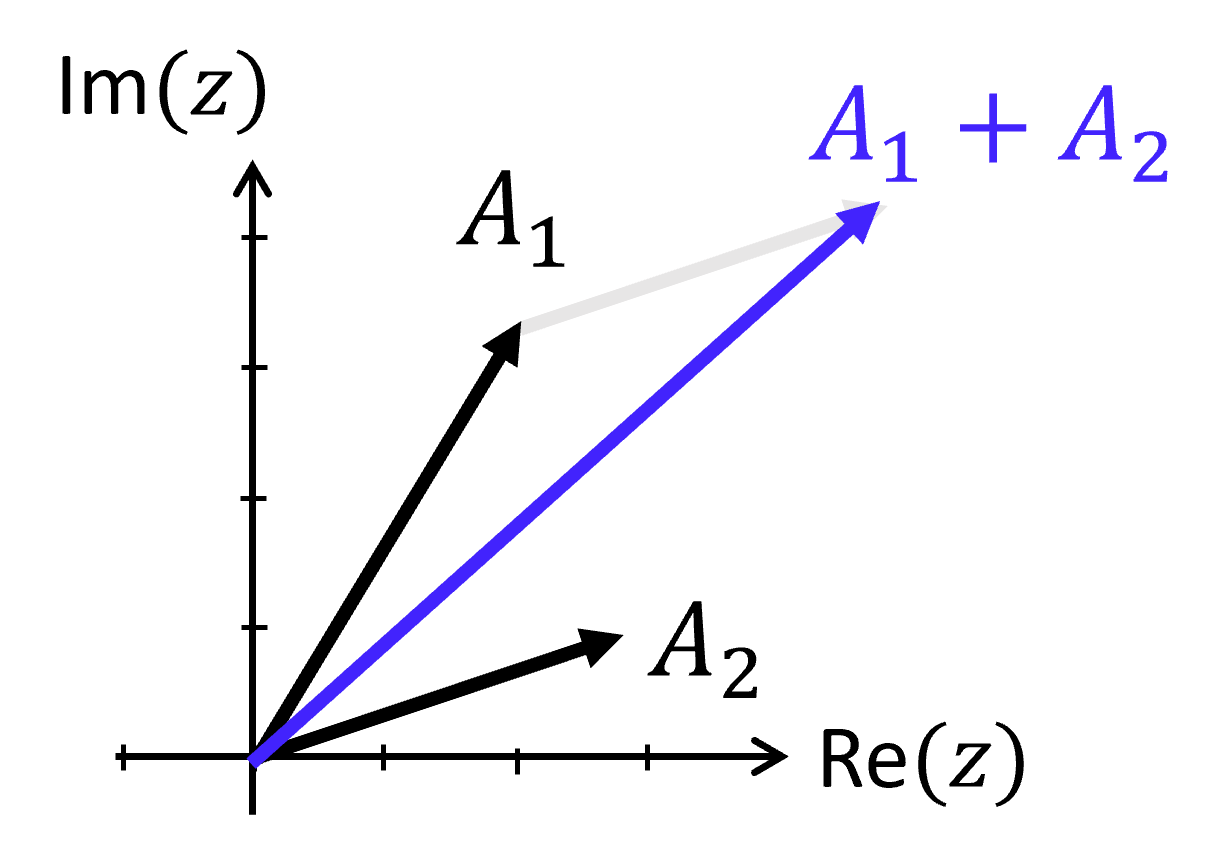
\includegraphics[width=\textwidth]{../Mathematik_1/Bilder/komplexe_zahlen_addition_komplexer_amplituden.png}
\end{minipage}
\begin{minipage}{0.58\textwidth}

Die komplexen Amplituden
\[
\underline A_1
\qquad\text{und}\qquad
\underline A_2
\]
werden als Pfeile in der komplexen Ebene dargestellt.

Ihre Summe
\[
\underline A
=
\underline A_1+\underline A_2
\]
entsteht durch Pfeiladdition.

Der Betrag des resultierenden Pfeils bestimmt die Amplitude der �berlagerten
Schwingung, sein Winkel bestimmt ihre Phase.

\end{minipage}

\end{exabox}


% --------------------------------------------------------------------------
\subsubsection*{Ein vollst�ndig gerechnetes Beispiel}

Betrachtet werden die beiden Schwingungen
\[
s_1(t)=\sin(\omega t)
\]
und
\[
s_2(t)
=
\sin\left(
\omega t+\frac{\pi}{2}
\right).
\]

F�r die erste Schwingung gilt \(A_1=1\) und \(\alpha_1=0\). Ihre komplexe
Amplitude ist daher
\[
\underline A_1
=
e^{i\cdot0}
=
1.
\]

F�r die zweite Schwingung gilt \(A_2=1\) und
\(\alpha_2=\pi/2\). Damit ergibt sich
\[
\underline A_2
=
e^{i\pi/2}
=
i.
\]

Die resultierende komplexe Amplitude lautet
\[
\underline A
=
\underline A_1+\underline A_2
=
1+i.
\]

Um daraus Amplitude und Phase der resultierenden Schwingung abzulesen, wird
\(1+i\) in Polarform dargestellt. Der Betrag ist
\[
A
=
|1+i|
=
\sqrt{1^2+1^2}
=
\sqrt2.
\]

Der Punkt \((1\,|\,1)\) liegt im ersten Quadranten und besitzt den Winkel
\[
\alpha
=
\frac{\pi}{4}.
\]
Damit gilt
\[
\underline A
=
\sqrt2\,e^{i\pi/4}.
\]

Die �berlagerung der beiden urspr�nglichen Schwingungen ergibt somit
\[
s(t)
=
\sqrt2
\sin\left(
\omega t+\frac{\pi}{4}
\right).
\]

Das Ergebnis zeigt unmittelbar den Vorteil der komplexen Darstellung. Anstatt
zwei trigonometrische Funktionen mithilfe von Additionstheoremen
zusammenzufassen, werden ihre komplexen Amplituden addiert. Betrag und Winkel
der resultierenden komplexen Zahl liefern anschlie�end Amplitude und Phase
der �berlagerten Schwingung.


% --------------------------------------------------------------------------
\subsection{Linearfaktorzerlegung �ber \(\mathbb C\)}

Die Einf�hrung der komplexen Zahlen begann mit einer algebraischen Frage:
Bestimmte Gleichungen besitzen innerhalb der reellen Zahlen keine L�sung.
Bereits eine quadratische Gleichung kann eine negative Diskriminante besitzen
und damit keine reellen Nullstellen haben.

In den komplexen Zahlen k�nnen solche Gleichungen weiter gel�st werden. So
besitzt beispielsweise
\[
z^2+6z+13=0
\]
die beiden komplexen L�sungen
\[
z_1=-3+2i
\qquad\text{und}\qquad
z_2=-3-2i.
\]

Damit l�sst sich das zugeh�rige Polynom vollst�ndig in Linearfaktoren
zerlegen:
\[
z^2+6z+13
=
(z+3-2i)(z+3+2i).
\]

Das Beispiel ist Teil eines wesentlich allgemeineren Zusammenhangs. W�hrend
ein reelles Polynom in \(\mathbb R\) nicht notwendigerweise eine Nullstelle
besitzt, ist die Situation �ber \(\mathbb C\) grundlegend anders.

\begin{theorembox}{Fundamentalsatz der Algebra}{ }

Jedes nichtkonstante Polynom mit komplexen Koeffizienten besitzt mindestens
eine komplexe Nullstelle.

Daraus folgt, dass sich jedes Polynom \(p\in\mathbb C[z]\) vom Grad
\(n\geq1\) vollst�ndig in Linearfaktoren zerlegen l�sst. Mit geeigneten
komplexen Zahlen \(z_1,\ldots,z_n\) gilt
\[
p(z)
=
a_n
(z-z_1)(z-z_2)\cdots(z-z_n).
\]

Dabei werden die Nullstellen entsprechend ihrer Vielfachheit gez�hlt. Ein
Polynom vom Grad \(n\) besitzt �ber \(\mathbb C\) somit genau \(n\)
Nullstellen, wenn Vielfachheiten ber�cksichtigt werden.

\end{theorembox}

F�r Polynome mit reellen Koeffizienten treten nichtreelle Nullstellen dabei
paarweise als komplex konjugierte Zahlen auf. Ist beispielsweise
\(a+i\,b\) mit \(b\neq0\) eine Nullstelle eines reellen Polynoms, so ist auch
\(a-i\,b\) eine Nullstelle.

Dies erkl�rt auch das vorangegangene Beispiel:
\[
-3+2i
\qquad\text{und}\qquad
-3-2i
\]
bilden ein komplex konjugiertes Paar.

Der Fundamentalsatz der Algebra schlie�t damit den Kreis zur urspr�nglichen
Motivation f�r die Einf�hrung der komplexen Zahlen. Die Erweiterung von
\(\mathbb R\) zu \(\mathbb C\) erm�glicht nicht nur die L�sung einzelner
Gleichungen wie \(z^2=-1\). Sie schafft einen Zahlenbereich, in dem jedes
nichtkonstante Polynom vollst�ndig in Linearfaktoren zerlegt werden kann.
 \newpage % Komplexe Zahlen Wurzeln und komplexe Exponentialfunktion
\setcounter{exercise}{0} 
\ifintegriereaufgaben
\section*{Komplexe Zahlen II Aufgaben}\label{MA1-komplexe-zahlen-polarform-und-euler-aufgaben}

	Regeln und Beispiele, die zur Bearbeitung der Aufgaben hilfreich sind, finden Sie im Skript\wennreferenzvorhanden{MA1-komplexe-zahlen-polarform-und-euler}{ (Abschnitt \abschnittsverweis{MA1-komplexe-zahlen-polarform-und-euler})} und, falls Sie nicht weiterkommen, dann schauen Sie \hyperref[MA1-komplexe-zahlen-polarform-und-euler-loesungen]{hier}.
\else 
\section{Komplexe Zahlen II Aufgaben}\label{MA1-komplexe-zahlen-polarform-und-euler-aufgaben}

	Regeln und Beispiele, die zur Bearbeitung der Aufgaben hilfreich sind, finden Sie im Skript und, falls Sie nicht weiterkommen, dann schauen Sie \hyperref[MA1-komplexe-zahlen-polarform-und-euler-loesungen]{hier}.
\fi 

%\begin{theorembox}[Polarform und kartesische Form]
%	Eine komplexe Zahl kann man in kartesischer Form, also $z=x+iy$ mit $x,y\in\mathbb R$ angeben, oder, falls $z\not=0$ in Polarform, also $z = r\cdot e^{i\varphi}$. Je nachdem was f�r eine Fragestellung zu l�sen ist, wird man sich f�r eine der beiden Darstellungen entscheiden. 
%	\begin{itemize} 
%		\item Wie kommt man von Polarform $z=r\cdot e^{i\varphi}$ f�r $r>0$ zur kartesischen Form?
%	\begin{eqnarray*} 
%		z =  x+ iy \quad \textnormal{mit}\; 
%		\begin{cases} 
%		x = r \cos(\varphi)\\
%		y = r \sin(\varphi)
%	\end{cases}
%	\end{eqnarray*}
%	\item Wie kommt man von kartesischen Form $z=x+iy$ zur Polarform?
%		\begin{eqnarray*} z=r\cdot e^{i\varphi} \quad \textnormal{mit} \; 
%	r=\sqrt{x^2+y^2}, \quad \varphi =\textnormal{atan2}(y,x): = 
%	\begin{cases} 
%		\arctan(y/x), \quad &x>0, \; y> 0\\[1ex]
%		\arctan(y/x), \quad& x>0, \; y< 0\\[1ex]
%		\arctan(y/x) + \pi, \quad& x<0, \; y\geq 0\\[1ex]
%		\arctan(y/x) - \pi, \quad& x<0, \; y< 0\\[1ex]
%		\pi/2, \quad & x=0, \; y> 0\\[1ex]
%		-\pi/2, \quad&  x<=0, \; y< 0\\[1ex]
%		0, \quad&  x<=0, \; y= 0
%	\end{cases}
%	\end{eqnarray*} 
%		\end{itemize}
%\end{theorembox}

\begin{exercisebox}[Radizieren]
	Bestimmen Sie alle L�sungen der folgenden Gleichungen
	\begin{eqnarray*}
		(a)\; z^3 = -8 \quad \quad \quad 
		(b)\; z^2 = i \quad \quad \quad  
		(c)\; z^4 = -16 
  \end{eqnarray*}
\end{exercisebox}

		\begin{exercisebox}[Eulersche Identit�t]
			Zeigen Sie, dass die folgenden Darstellungen f�r $\sin$ und $\cos$ gelten
			\begin{eqnarray*} 
				(a)\; \sin(\varphi) = \frac{e^{i\varphi} - e^{-i\varphi}}{2i} \quad\quad\quad (b)\;\cos(\varphi) = \frac{e^{i\varphi} + e^{-i\varphi}}{2} 
			\end{eqnarray*}
		\end{exercisebox}

\begin{exercisebox}[Fundamentalsatz]
	Betrachten Sie f�r $n\in \mathbb N$ ein Polynom \[ p:\mathbb C\to \mathbb C, \; z\mapsto p(z)=a_nz^n+a_{n-1}z^{n-1} +\cdots a_1z+a_0\] mit reellen Koeffizenten $a_0, \cdots, a_n\in \mathbb R$ und $a_n\not=0$. 
	\begin{itemize}
		\item[(a)] Zeigen Sie: wenn $z_0 \in \mathbb C$ eine Nullstelle von $p$ ist, dann ist auch $\overline{z_0}$ eine Nullstelle von $p$.
		\item[(b)] Wenden Sie obigen Satz an, um alle Nullstellen des Polynoma \[ p:\mathbb C\to \mathbb C, \; z\mapsto p(z) = z^4-2z^3+2z^2-10z+25 \] zu bestimmen. Zeigen Sie zu erst, dass $z_1= 2+j$ eine Nullstelle ist.
	\end{itemize}
\end{exercisebox}

\begin{exercisebox}[Fundamentalsatz]
	\begin{itemize}
		\item[(a)]
	L�sen Sie die Gleichung: $4z^2 + (8+12i)z - 5+11i = 0$.
	%\begin{eqnarray*}
	%	p(z) &=& \underbrace{4}_{a_2}z^2 + \underbrace{(8+12i)}_{a_1}z \underbrace{- 5+11i}_{a_0} \\
	%	&=& (2z)^2 + 2\cdot 2z \cdot (2+3i) + (2+3i)^2 -(2+3i)^2-5+11i \\
	%	&=& (2z+2+3i)^2-i \\
	%	&&\\
	%	\Rightarrow && (2z+2 + 3i)^2 = i = 1\cdot e^{i\pi/2} \Rightarrow\begin{cases} 2z_0+2+3i = \frac{\sqrt{2}}{2} + i\frac{2}{2} \\ 2z_1+2+3i = -\frac{\sqrt{2}}{2} - i\frac{2}{2} \end{cases}
	%		\end{eqnarray*}
\item[(b)] Bestimmen Sie alle Nullstellen des komplexen Polynoms $p:z\mapsto z^2+\left(2\sqrt{2}i\right) \cdot z - 2\sqrt{3} i$.
	\end{itemize}
\end{exercisebox}

\begin{exercisebox}[Anwendungen: Additionstheoreme]
	Zeigen Sie, dass f�r alle $x\in \mathbb R$ gilt
	\begin{eqnarray*}
	(a)\; \sin(x \pm y) = \sin(x)\cdot \cos(y) \pm \cos(x)\cdot\sin(y),\quad \quad (b)\; \cos(3x) = 4 (\cos(x))^3 - 3\cos(x) 
\end{eqnarray*}
\end{exercisebox}

\begin{exercisebox}[Anwendungen: Harmonische Schwingungen]
	Gegeben seien die harmonischen Schwingungen \[ s_1(t) = \sqrt{2} \cdot \sin(10t+\pi/4), \quad s_2(t)=2\cos(10t+\pi/6)\,.\]
	\begin{itemize}
		\item[(a)] Berechnen Sie die �berlagerung von $s_1$ und $s_2$. 
			
			Hinweis: $\sin(t) =  \mathrm{Im}\left( e^{i\,t}\right), \;\cos(\omega\,t) = \sin(\omega\, t + \pi/2) $. 
		\item[(b)] Wie muss eine harmonische Schwingung \[ s_3(t) = A_3\sin(\omega_3 t+ \varphi_3)\] gew�hlt werden, dass die �berlagerung von $s_1$ und $s_3$ eine Amplitude von $1$ und eine Nullphase von $\pi/2$ besitzt?
	\end{itemize}
\end{exercisebox}
 \newpage 
\setcounter{satz}{0} \setcounter{def}{0} \setcounter{exa}{0}  \section{Vektoren}\label{MA1-vektoren}

\begin{table}[H]
  \centering
  \begin{tabularx}{\textwidth}{p{0.9\textwidth} p{0.1\textwidth}}
    \toprule
	  \multicolumn{2}{c}{\textbf{�bersicht �ber Lernziele und Voraussetzungen}}\\
    \midrule
\textbf{Lernziele} &\\[.5\normalbaselineskip]
\tabitem Vektoren in \(\mathbb R^n\) und \(\mathbb C^n\) darstellen, addieren und skalieren &\\
\tabitem die Norm eines Vektors berechnen und Einheitsvektoren bestimmen &\\
\tabitem das Skalarprodukt berechnen und geometrisch interpretieren &\\
\tabitem Orthogonalit�t mithilfe des Skalarprodukts pr�fen &\\
\tabitem Vektoren orthogonal zerlegen und auf eine vorgegebene Richtung projizieren &\\
\tabitem den Winkel zwischen zwei reellen Vektoren mithilfe des Skalarprodukts bestimmen &\\
\tabitem Norm und Skalarprodukt auf Vektoren in \(\mathbb C^n\) �bertragen (+) &\\
\tabitem das Kreuzprodukt in \(\mathbb R^3\) berechnen und geometrisch interpretieren (+) &\\
    \midrule
	  \textbf{Voraussetzungen} &\\[.5\normalbaselineskip]
	  \tabitem Grundlagen & \abschnittsverweis{MA1-mengen-und-logik}-\abschnittsverweis{MA1-aequivalenzumformungen}\\
	  \tabitem Geometrie rechtwinkliges Dreieck & \abschnittsverweis{MA1-trigonometrische-funktionen}\\
	  \tabitem Komplexe Zahlen & \abschnittsverweis{MA1-komplexe-zahlen-grundlagen}\\
    \bottomrule
  \end{tabularx}
\end{table}

\ifintegriereaufgaben \noindent �bungsaufgaben zum Thema finden Sie hier: \hyperref[MA1-vektoren-aufgaben]{Aufgaben}
\vspace{0.3cm}
\hrule
\fi

\subsection{Was ist ein Vektor?} % Kapitel fr�her 

Pfeile kann man addieren und subtrahieren und man kann die L�nge von Pfeilen durch Multiplikation mit Zahlen ver�ndern:
\begin{exabox}{Pfeile}{ }
\begin{minipage}{0.5\textwidth}
	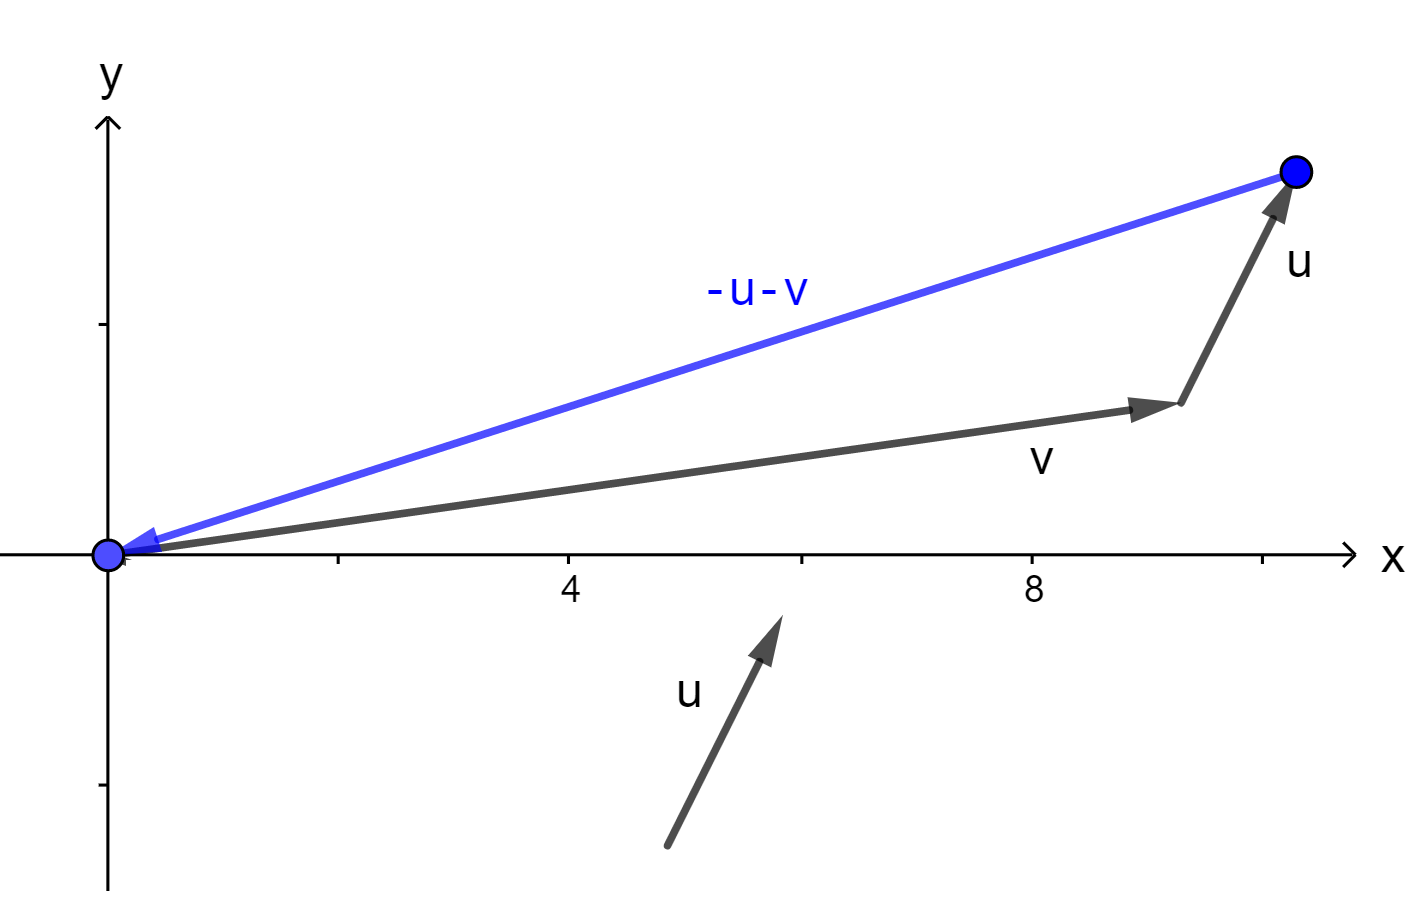
\includegraphics[width=\textwidth]{../Mathematik_1/Bilder/vektoren_pfeiladdition_gegenvektor.png}
\end{minipage}
\begin{minipage}{0.5\textwidth}
		Pfeilarithmetik kann man in \(\mathbb R^2\) gut skizzieren:
	\[ - (\vec v+\vec u) = -\vec v - \vec u  \]
\end{minipage}
\end{exabox}

Das klappt in zwei Dimensionen (Ebene) ebenso wie in drei Dimensionen (Raum). Ein Pfeil wird vollst�ndig durch seine L�nge und seine Richtung beschrieben. Um die Operation "\,Addition"\, komplett zu haben, ben�tigt man ein \underline{neutrales Element}\randverweis{MA1-zahlenmengen} der Addition. Das neutrale Element der Addition ist ein Pfeil mit L�nge Null und unbestimmter Richtung, der sogenannte Nullpfeil $\vec 0$. Es gilt: \[ \forall\, \vec a: \quad \vec a+ \vec 0= \vec a\,.\]

Zwei Pfeile werden mathematisch als gleich betrachtet, wenn sie in L�nge und Richtung �bereinstimmen: mathematisch unterscheiden sich also zwei parallel gegeneinander verschobene Pfeile nicht. Es handelt sich in der Mathematik um einen \textbf{Vektor} (\emph{vector}):
\begin{exabox}{Vektoren}{ }
\begin{minipage}{0.3\textwidth}
	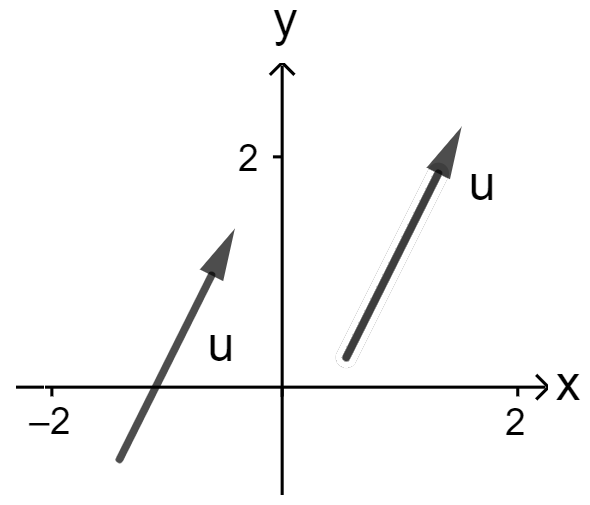
\includegraphics[width=\textwidth]{../Mathematik_1/Bilder/vektoren_gleiche_pfeile_verschoben.png}
\end{minipage}
\begin{minipage}{0.7\textwidth}
	Ein Vektor in der Mathematik ist durch die Angabe
	\begin{itemize}
		\item seiner L�nge und 
		\item seiner Richtung 
	\end{itemize}
	eindeutig bestimmt. Man darf den Vektor in der Ebene beliebig verschieben, es sind unbebundene Vektoren. 
\end{minipage}
\end{exabox}


Zwei- und dreidimensionale Vektoren werden orthographisch meist mit einem Pfeil oder unterstrichen dargestellt, also $\vec a$ oder $\underline a$, oder mit Fettbuchstab $\boldsymbol a$. Je abstrakter die Vektoren werden, um so eher benutzt man normale Buchstaben wie $a$. 

Die Vokabeln \"\,Vektor\"\, und \"\,Skalar\"\, werden nicht nur in mathematischen Zusammenh�ngen, sondern auch in der Physik st�ndig auftauchen. Es ist sinnvoll die Unterschiede zu erkl�ren:  


\vspace{0.3cm}
\noindent\textbf{Vektoren und Skalare in der Mathematik}
\begin{itemize}
	\item Vektoren in der Mathematik sind ungebundene bzw. freie Vektoren. Das Adjektiv "\,frei"\, betont, dass zwei parallele gleichlange Vektoren dieselben mathematischen Objekte sind.  
	\item Vektoren mit fixiertem Start- oder Aufh�ngepunkt \(P\) nennt man in der Mathemamtik gebundene Vektoren: 
	\item Skalare in der Mathematik sind die Zahlen, mit denen man Vektoren multiplizieren kann: also reelle oder komplexe Zahlen. Multipliziert man einen Vektor mit einer Zahl, so ver�ndert man seine L�nge, aber nicht seine Richtung - man spricht auch von Skalierung.  
\end{itemize}

\noindent\textbf{Vektoren und Skalare in der Physik}
\begin{itemize}
	\item Vektoren in der Physik sind vektorielle Gr��en wie beispielsweise der Geschwindigkeitsvektor \(\vec v\), der Impulsvektor \(\vec p\), das elektrostatische Feld \(\vec E\) oder die Newtonsche Kraft \(\vec F\)\ldots 
	\item Vektoren in der Physik, die an einem fixierten Punkt \(P\) starten, nennt man Ortsvektoren $ P + \vec v\,.$
	\item Skalare in der Physik sind ungerichtete Gr��en, beispielsweise die Masse \(m\) eines K�rpers, die Anzahl \(N\) von Teilchen, die Ladung \(q\) eines Atoms, die Energie \(E\) eines Systems oder die Raumtemperatur \(T\)\ldots 
	\item Physikalische Gr��en k�nnen nicht nur gerichtet (vektoriell) oder ungerichtet (skalar), sondern auch komplizierter sein. Zur Beschreibung der Drehung eines massebehafteten Objektes um eine bestimmte Achse braucht man den sogennanten Tr�gheitstensor \(I\). Ein Tr�gheitstensor ist kein Vektor und es ist kein Skalar, sondern eine \underline{Matrix}\randverweis{MA1-matrizen}.
	\item Jede physikalische Gr��e, ob skalar, vektoriell oder tensorwertig, besteht aus einem Zahlenwert und einer Ma�einheit. Wenn man physikalische Gesetze aufschreibt und mit physikalischen Gr��en rechnet, dann kann man immer nur Gr��en gleicher Einheit miteinander verrechnen. Deshalb ist es immer hilfreich einen Vergleich der Einheiten zu machen -  so findet man schnell heraus, ob eine Formulierung sinnvoll oder unm�glich ist:
\begin{itemize}
	\item eine Masse von $m=2.3 \, [\mathrm{ kg}]$ kann nicht mit einem Zeitintervall der L�nge $\delta t=2.3\, [\mathrm{s}]$ gleichgesetzt werden,
	\item ein Beschleunigungsvektor $\vec a = (4.2,0,0)^\intercal \, [\frac{m}{s^2}]$ kann nicht dem sklaren Druck $p=4.2\, [\mathrm{Pa}]$ entsprechen,
	\item ein Kraftvektor $\vec F \; [\mathrm{N}] = [\frac{\mathrm{kg}\cdot \mathrm{m}}{\mathrm{s}^2}]$, kann nicht gleich einem Geschwindigkeitsvektor $\vec v \; [\frac{\mathrm{m}}{\mathrm{s}}]$ sein.
\end{itemize} 
\end{itemize}

Um mit Vektoren sinnvoll rechnen zu k�nnen, dr�ckt man sie in Zahlen aus. Der Vektor, der eine Einheit nach links und drei nach oben zeigt lautet beispielsweise 
\begin{defbox}{Komponenten eines Vektors}{ }
	Ein Vektor, der eine Einheit nach links und drei nach oben zeigt lautet 
	\[ \vec a=\left( \begin{array}{c} -1 \\ 3\end{array} \right)\,. \]  
		Die Zahlen \(-1\) und \(3\) nennt man Komponenten oder Koeffizienten oder auch Eintr�ge des Vektors. 
	Entsprechend haben Vektoren im Raum drei Komponenten, beispielsweise
\[  \vec a = \left( \begin{array}{c} 2 \\ 3 \\ -4\end{array} \right)\,. \]
\end{defbox} 

Die Komponenten eines Vektors schreibt man meistens senkrecht untereinander, also als Spalte. So entsteht ein \textbf{Spaltenvektor}. Werden die Komponenten in eine Zeile geschreiben, dann spricht man von einem \textbf{Zeilenvektor}. Ein Spaltenvektore wird durch \textbf{Transposition} in einen Zeilenvektor umgewandelt. Das kleine Symbol \(^\intercal\) zeigt die Drehung an: 

\[ \left(  -1, 3\right)^\intercal = \left( \begin{array}{c} -1 \\3\end{array}\right) \quad \textnormal{bzw.} \quad \left(  2, 3, -4\right)^\intercal = \left( \begin{array}{c} 2 \\ 3 \\ -4\end{array}\right)\,. \]  

\begin{exabox}{Rechnen mit Vektoren in der Ebene}{ }
	\begin{itemize}
		\item Man skaliert einen Vektor, indem man jede Komponente des Vektors mit dem Skalar multipliziert:  
\[ 
	2 \cdot \vec a= 2\cdot \left( \begin{array}{c} -1 \\ 3\end{array} \right) = \left( \begin{array}{c} 2\cdot (-1) \\ 2\cdot 3\end{array} \right) = \left( \begin{array}{c} -2 \\ 6\end{array} \right)\,.
\]
\item Man addiert zwei Vektoren, indem man die Komponenten der Vektoren zeilenweise addiert: 
  \[  
  \vec a + \vec b = \left( \begin{array}{c} -1 \\ 3\end{array} \right)  + \left( \begin{array}{c} 4 \\ 2\end{array} \right) =  \left( \begin{array}{c} 3 \\ 5\end{array} \right) \,.
  \]
	\end{itemize}
\end{exabox} 

\noindent\textbf{Bemerkungen:}
\begin{itemize}
	\item Die Bedeutung der Komponenten h�ngt von der Wahl des Ursprungs und der Achsen ab! 
	\item Der Nullvektor $\vec 0$ ist der Vektor, bei dem alle Komponenten gleich null sind.
\end{itemize}

Die Menge aller Vektoren mit zwei reellen Komponenten wird mit $\mathbb R^2$ bezeichnet und die Menge aller Vektoren mit drei reellen Komponenten ist entsprechend $\mathbb R^3$.
Allgemein schreibt man
\[
\mathbb R^n = \mathbb R \times \mathbb R \times \dots \times \mathbb R ,
\]
das sogenannte $n$-fache kartesische Produkt der reellen Zahlen.

Das Wort "\,identifizieren"\, resultiert aus der Tatsache, dass die Mengen $\mathbb R^n, \; n \in \mathbb N^+$, ein Doppelleben f�hren: man kann jedes Element des $\mathbb R^2$ entweder als Punkt $(x\,|\,y)$ in der Ebene oder als Vektor $(x,y)^\intercal$ auffassen. 
\begin{defbox}{$\mathbb R^2$ als Menge von Vektoren}{ }
	\[ \mathbb R^2 = \left\{ \left( \begin{array}{c}  x \\ y \end{array}\right)\, \textnormal{mit}\; x,y\in \mathbb R\right\} \]
\end{defbox}
Aus dem Zusammenhang wird klar, welchen Standpunkt man einnimmt. %Im Englisch sprachigen Raum schreibt man Punkte in der Form $(2,3)$, was im Deutschen zu Verwechselungen mit dem Dezimalkomma f�hren kann.
Die einfachste �bersetzung zwischen Punkten und Vektoren ergibt sich wie folgt
\begin{exabox}{Vektor vs. Punkt}{ }
	$ \left( \begin{array}{c}  2 \\ 3 \end{array}\right) = (2\, | \,3) - (0\,|\,0)\,, $
\end{exabox}
wobei nun links explizit ein gebundener Vektor mit Aufh�ngepunkt im Ursprung steht.

Kommen wir nochmal zur�ck auf die Definition eines Vektors: ein freier Vektor ist durch seine L�nge und seine Richtung eindeutig bestimmt. Das bedeutet, dass die Angabe dieser Informationen gen�gt, um den Vektor zu kennen! 
\[ \textnormal{Vektor}\quad   \Leftrightarrow \quad  \left( \,\textnormal{L"ange, Richtung} \,\right) \]
F�r die L�nge $\| \vec a\| $ oder $|\vec a|$ eines  Vektors $\vec a\in\mathbb R^2$ gilt\marginpar{\small Warum?}:
  \[
  \begin{array}{rcl}
	  \vec a = \left( \begin{array}{c} 2 \\ -4\end{array} \right) \quad \Rightarrow \|\vec a\| := \sqrt{ 2^2+(-4)^2} = \sqrt{20} \,.
\end{array}
\]
Zur Angabe der Richtungsinformation von \(\vec a\) bietet sich ein Vektor an, der in Richtung von \(\vec a\) zeigt und dessen L�nge zu eins normiert ist, der also keine spezifische L�ngeninformation �ber \(\vec a\) besitzt! 

\begin{defbox}{Einheitsvektor}{ }
	Zu einem gegebenen Vektor \(\vec a \not = \vec 0\) ist \(\hat a\) der zugeh�rigen \textbf{Einheitsvektor}, wobei
$$
\hat a:= \dfrac{\vec a}{\|\vec a\|}\,.
$$
\end{defbox}

Das Konzept der Vektoren in der Ebene ist sehr zug�nglich, weil wir uns die Vektoren vorstellen k�nnen. Allerdings hindert uns nichts daran das Konzept zu erweitern, beispielsweise auf \(\mathbb R^n\).  

\begin{defbox}{Vektoren in \(\mathbb R^n\) }{ }
	Ein \(n\)-Tupel reeller Zahlen \(a_k, \, k=1,\dots,n\) definiert einen Vektor in \(\mathbb R^n\) mit \(n\) Komponenten: 
\[  \vec a = \left( a_1, a_2, \cdots, a_n\right)^\intercal\,. \]
Ein nicht-trivialer Vektor, \(\vec a \not = \vec 0\), ist durch seine L�nge und seine Richtung eindeutig festgelegt:
\[ \vec a\quad   \Leftrightarrow \quad  \left( \|\vec a\| ,  \hat a\right)\,, \quad \textnormal{mit}\quad \begin{cases}\left\| \vec a \right\| &= \displaystyle{\sqrt{ \sum\limits_{k=1}^n a_k^2}} \geq 0\in \mathbb R\,, \\ \hat a &= \dfrac{\vec a}{\|\vec a\|}\,,\end{cases}\]
und es gilt 
\[ \vec a = \|\vec a\| \cdot\hat a\,.\]
\end{defbox}

\subsection{Skalarprodukt}

Vektoren k�nnen addiert und mit Skalaren multipliziert werden. Damit lassen
sich bereits viele geometrische Operationen algebraisch beschreiben. Eine
wesentliche geometrische Information ist damit jedoch noch nicht unmittelbar
zug�nglich: die Lage zweier Vektoren relativ zueinander.

Insbesondere stellt sich die Frage, wie algebraisch erkannt werden kann, ob
zwei Vektoren in dieselbe Richtung zeigen, senkrecht aufeinander stehen oder
einen bestimmten Winkel miteinander einschlie�en.

Eine solche Information kann nicht durch Addition oder skalare
Multiplikation allein gewonnen werden. Daf�r wird eine weitere Verkn�pfung
ben�tigt, die zwei Vektoren eine Zahl zuordnet. Diese Verkn�pfung ist das
\textbf{Skalarprodukt} (\emph{inner product}).

Auch in der Physik tritt genau eine solche Verkn�pfung auf. Bei der
mechanischen Arbeit ist nicht nur die Gr��e einer Kraft und eines Weges
entscheidend, sondern auch deren relative Richtung. Eine Kraft, die senkrecht
zur Bewegungsrichtung wirkt, verrichtet entlang dieses Weges keine Arbeit.
Das Skalarprodukt erfasst genau diese Richtungsinformation.

\begin{defbox}{Skalarprodukt in \(\mathbb R^n\)}{ }

F�r zwei Vektoren
\[
\vec a
=
(a_1,\ldots,a_n)^\intercal,
\qquad
\vec b
=
(b_1,\ldots,b_n)^\intercal
\]
in \(\mathbb R^n\) ist das Skalarprodukt definiert durch
\[
\langle\vec a,\vec b\rangle
=
\sum_{k=1}^{n}a_kb_k.
\]

Das Ergebnis des Skalarprodukts ist \emph{kein} Vektor, sondern eine reelle
Zahl:
\[
\langle\vec a,\vec b\rangle\in\mathbb R.
\]

\noindent\textbf{Bemerkung zur Schreibweise:}
F�r das Skalarprodukt sind verschiedene Schreibweisen gebr�uchlich. Neben
\(\langle\vec a,\vec b\rangle\) wird insbesondere auch ein ausgef�llter
Punkt verwendet oder ein kleines Malzeichen,
\[
	\vec a\bullet\vec b, \quad  \vec a \cdot \vec b\,.
\]
\end{defbox}

Die Berechnung erfolgt komponentenweise. Entsprechende Komponenten werden
multipliziert und die entstehenden Produkte anschlie�end addiert. F�r
\[
\vec a
=
\begin{pmatrix}
3\\4\\5
\end{pmatrix},
\qquad
\vec b
=
\begin{pmatrix}
2\\-3\\1
\end{pmatrix}
\]
ergibt sich beispielsweise
\[
\langle\vec a,\vec b\rangle
=
3\cdot2+4\cdot(-3)+5\cdot1
=
-1.
\]

Neben der Schreibweise
\(\langle\vec a,\vec b\rangle\) ist insbesondere in
\(\mathbb R^n\) auch die Schreibweise
\(\vec a\cdot\vec b\) gebr�uchlich.


\begin{theorembox}{Eigenschaften des Skalarprodukts}{ }

F�r \(\vec a,\vec b,\vec c\in\mathbb R^n\) und
\(\lambda\in\mathbb R\) gilt
\[
\langle\vec a,\vec b\rangle
=
\langle\vec b,\vec a\rangle,
\]
\[
\langle\vec a,\vec b+\vec c\rangle
=
\langle\vec a,\vec b\rangle
+
\langle\vec a,\vec c\rangle
\]
sowie
\[
\langle\lambda\cdot \vec a,\vec b\rangle
=
\langle\vec a,\lambda\cdot \vec b\rangle
=
\lambda\cdot \langle\vec a,\vec b\rangle.
\]

Das reelle Skalarprodukt ist damit symmetrisch und linear in beiden
Argumenten.

\end{theorembox}


\subsubsection*{Skalarprodukt und L�nge}

Eine erste Verbindung zwischen dem Skalarprodukt und der Geometrie entsteht,
wenn ein Vektor mit sich selbst multipliziert wird. F�r
\(\vec a\in\mathbb R^n\) gilt
\[
\langle\vec a,\vec a\rangle
=
a_1^2+\cdots+a_n^2.
\]
Der Ausdruck auf der rechten Seite ist gerade das Quadrat der euklidischen
L�nge von \(\vec a\).

\begin{theorembox}{Relation zwischen Norm und Skalarprodukt}{ }

F�r jeden Vektor \(\vec a\in\mathbb R^n\) gilt
\[
\|\vec a\|^2
=
\langle\vec a,\vec a\rangle
\]
und damit
\[
\|\vec a\|
=
\sqrt{\langle\vec a,\vec a\rangle}.
\]

\end{theorembox}

Das Skalarprodukt enth�lt damit bereits die Information �ber die L�nge eines
Vektors. Entscheidend ist jedoch, dass es dar�ber hinaus auch die relative
Richtung zweier verschiedener Vektoren erfasst.

\subsubsection*{Projektion und Winkel zwischen Vektoren}

Orthogonalit�t beschreibt zun�chst nur den besonderen Fall eines Winkels von
\(90^\circ\). In der Ebene und im dreidimensionalen Raum l�sst sich jedoch
auch der Winkel zwischen zwei beliebigen Vektoren geometrisch betrachten.

Ausgangspunkt ist zun�chst die anschauliche Situation in der Ebene. Gesucht
ist der Anteil eines Vektors \(\vec b\), der in Richtung eines zweiten
Vektors \(\vec a\) zeigt. Dazu wird \(\vec b\) in zwei zueinander
orthogonale Anteile zerlegt: einen Anteil \(\vec b_{\parallel}\), der
parallel zu \(\vec a\) verl�uft, und einen Anteil \(\vec b_{\perp}\), der
senkrecht auf \(\vec a\) steht.

\vspace{0.5cm}
\begin{center}
\begin{minipage}{0.3\textwidth}
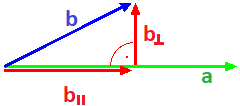
\includegraphics[width=\textwidth]{../Mathematik_1/Bilder/vektoren_orthogonale_zerlegung.png}
\end{minipage}
\begin{minipage}{0.6\textwidth}
\[
\textcolor{blue}{\vec b}
=
\textcolor{red}{\vec b_{\parallel}}
+
\textcolor{red}{\vec b_{\perp}},
\qquad
\left\langle
\textcolor{red}{\vec b_{\perp}},
\textcolor{darkgreen}{\vec a}
\right\rangle
=
0.
\]
\end{minipage}
\end{center}
\vspace{0.5cm}

Der parallele Anteil enth�lt genau die Information dar�ber, wie stark
\(\vec b\) in Richtung von \(\vec a\) zeigt.

Zun�chst seien \(\vec a,\vec b\in\mathbb R^2\) zwei von Null verschiedene
Vektoren und \(\alpha\in[0,\pi]\) ihr geometrisch eingeschlossener Winkel.
Ist \(\alpha\) spitz, so zeigt der parallele Anteil in Richtung von
\(\vec a\). Seine L�nge betr�gt nach der bekannten Geometrie des
rechtwinkligen Dreiecks \(\|\vec b\|\cos(\alpha)\). Mit dem Einheitsvektor
\(\hat a=\vec a/\|\vec a\|\) folgt daher
\[
\vec b_{\parallel}
=
\|\vec b\|\cos(\alpha)\,\hat a
=
\frac{\|\vec b\|}{\|\vec a\|}
\cos(\alpha)\,\vec a.
\]

Bei einem stumpfen Winkel ist \(\cos(\alpha)<0\). Der parallele Anteil zeigt
dann entgegen der Richtung von \(\vec a\). Dieselbe Formel beschreibt somit
beide F�lle.

Diese geometrische Zerlegung erm�glicht nun, das Skalarprodukt zu
interpretieren. Da
\(\vec b=\vec b_{\parallel}+\vec b_{\perp}\) und
\(\vec b_{\perp}\perp\vec a\), gilt
\[
\begin{array}{rcl l}
\big\langle\vec a,\vec b\big\rangle
&=&
\big\langle\vec a,\vec b_{\parallel}+\vec b_{\perp}\big\rangle & \quad \text{Orthogonale Zerlegung f�r } \vec b \text{ einsetzen} \\[0.5ex]
&=& \big\langle\vec a,\vec b_{\parallel}\big\rangle + \underbrace{\big\langle\vec a,\vec b_{\perp}\big\rangle}_{\displaystyle{=0} } & \quad \text{Eigenschaften des Skalarprodukts ausnutzen}\\[0.5ex]
&=& \big\langle \vec a, \frac{\|\vec b\|}{\|\vec a\|} \cdot \cos(\alpha)\cdot \vec a \big\rangle &\quad \text{Darstellung f�r } \vec b_\parallel \text{ einsetzen}\\[0.5ex] 
&=& \frac{\|\vec b\|}{\|\vec a\|}\cdot \cos(\alpha)\cdot \underbrace{\langle\vec a,\vec a\rangle}_{=\|\vec a\|^2} &\quad \text{Eigenschaften des Skalarprodukts ausnutzen} \\[0.5ex]
&=& \|\vec a\|\cdot\|\vec b\|\cdot \cos(\alpha). & \end{array}
\]

Damit ist f�r Vektoren in der Ebene eine Verbindung zwischen dem geometrisch bekannten Winkel und dem algebraisch berechenbaren Skalarprodukt gefunden:
\[
\cos(\alpha) = \frac{\langle\vec a,\vec b\rangle}{\|\vec a\|\cdot \|\vec b\|}.
\]

Diese Formel besitzt eine weitergehende Bedeutung. Ihre rechte Seite enth�lt nur das Skalarprodukt und die Norm der beiden Vektoren. Beide Begriffe sind bereits f�r Vektoren in \(\mathbb R^n\) definiert und ben�tigen keine zweidimensionale geometrische Darstellung.

Damit kann der aus der Ebene bekannte Winkelbegriff auf beliebige reelle Vektorr�ume \(\mathbb R^n\) �bertragen werden.

\begin{defbox}{Winkel zwischen Vektoren in \(\mathbb R^n\)}{ }

F�r zwei von Null verschiedene Vektoren
\(\vec a,\vec b\in\mathbb R^n\) wird der \textbf{Winkel}
\(\alpha\in[0,\pi]\) zwischen den beiden Vektoren durch
\[
\cos(\alpha)
:=
\frac{\langle\vec a,\vec b\rangle}
{\|\vec a\|\,\|\vec b\|}
\]
definiert.

�quivalent dazu gilt
\[
\alpha
=
\arccos\left(
\frac{\langle\vec a,\vec b\rangle}
{\|\vec a\|\,\|\vec b\|}
\right).
\]

F�r \(n=2\) und \(n=3\) stimmt diese Definition mit dem geometrisch
anschaulichen Winkel zwischen zwei Vektoren �berein.

\end{defbox}

Die Definition erweitert damit einen aus der ebenen und r�umlichen Geometrie
bekannten Begriff auf Dimensionen, in denen eine unmittelbare geometrische
Vorstellung nicht mehr zur Verf�gung steht. Ein Winkel zwischen zwei
Vektoren in \(\mathbb R^{10}\) oder \(\mathbb R^{100}\) l�sst sich nicht mehr
als Winkel zweier gezeichneter Pfeile veranschaulichen; �ber das
Skalarprodukt ist er dennoch eindeutig definiert.

%Die Winkelformel ist damit in der Ebene eine Konsequenz der geometrischen Interpretation des Skalarprodukts und wird anschlie�end zur Definition des Winkelbegriffs in \(\mathbb R^n\).

Gleichzeitig liefert dieselbe Beziehung die \textbf{vorzeichenbehaftete
Projektionsl�nge} von \(\vec b\) in Richtung von \(\vec a\). F�r den
Einheitsvektor \(\hat a\) gilt
\[
\langle\vec b,\hat a\rangle
=
\|\vec b\|\cos(\alpha).
\]
Dieser Wert beschreibt, wie stark \(\vec b\) in Richtung von
\(\vec a\) beziehungsweise bei negativem Vorzeichen in die
entgegengesetzte Richtung zeigt.

\begin{theorembox}{Orthogonale Projektion auf eine Richtung}{ }

F�r \(\vec a\neq\vec 0\) l�sst sich \(\vec b\) orthogonal zerlegen als
\[
\vec b
=
\vec b_{\parallel}
+
\vec b_{\perp} \quad \text{ mit } \vec b_{\perp}\perp\vec a.
\]
Der zu \(\vec a\) parallele Vektor ist
\[
\vec b_{\parallel}
=
\langle\vec b,\hat a\rangle\cdot \hat a
=
\frac{\langle\vec b,\vec a\rangle}
{\|\vec a\|^2} \cdot \vec a
\]
und der zu \(\vec a\) orthogonale Vektor ist
\[
\vec b_{\perp}
=
\vec b-\vec b_{\parallel}.
\]

\end{theorembox}

Das Skalarprodukt beantwortet damit mehrere zun�chst unterschiedliche
geometrische Fragen mit derselben algebraischen Operation: Es beschreibt
Orthogonalit�t, erm�glicht die orthogonale Projektion und erweitert den
geometrischen Winkelbegriff auf Vektoren in beliebigen Dimensionen.

Die Projektion wird sp�ter noch eine weitergehende Bedeutung erhalten. Wird
nicht nur auf eine einzelne Richtung, sondern auf einen ganzen Unterraum
projiziert, entsteht dort die bestm�gliche orthogonale Approximation eines
Vektors.

\subsubsection*{Vektoren in \(\mathbb C^n\)}

Die bisherigen �berlegungen bezogen sich auf Vektoren mit reellen
Komponenten. Nach der Einf�hrung der komplexen Zahlen liegt es nahe, auch
Vektoren
\[
\vec u
=
(u_1,\ldots,u_n)^\intercal
\in\mathbb C^n
\]
zu betrachten.

Addition und skalare Multiplikation werden wie in \(\mathbb R^n\)
komponentenweise durchgef�hrt. Bei der �bertragung des Skalarprodukts ist
jedoch eine Anpassung notwendig. W�rden komplexe Komponenten einfach
miteinander multipliziert, w�re insbesondere
\(\langle\vec u,\vec u\rangle\) im Allgemeinen keine
nichtnegative reelle Zahl und k�nnte daher nicht als Quadrat einer L�nge
interpretiert werden.

Deshalb wird eine der beiden Komponenten im Skalarprodukt komplex konjugiert.

\begin{defbox}{Skalarprodukt und Norm in \(\mathbb C^n\)}{ }

F�r
\[
\vec u
=
(u_1,\ldots,u_n)^\intercal,
\qquad
\vec v
=
(v_1,\ldots,v_n)^\intercal
\]
in \(\mathbb C^n\) wird das Skalarprodukt hier durch
\[
\langle\vec u,\vec v\rangle
=
\sum_{k=1}^{n}\overline{u_k}\,v_k
\]
definiert.

F�r die Norm folgt
\[
\|\vec u\|
=
\sqrt{\langle\vec u,\vec u\rangle}
=
\sqrt{
\sum_{k=1}^{n}|u_k|^2
}.
\]

\end{defbox}

Im Unterschied zum reellen Skalarprodukt ist das komplexe Skalarprodukt im
Allgemeinen nicht symmetrisch, sondern \textbf{konjugiert symmetrisch}:
\[
\langle\vec u,\vec v\rangle
=
\overline{
\langle\vec v,\vec u\rangle
}.
\]

Mit der hier verwendeten Konvention ist es im ersten Argument
konjugiert-linear und im zweiten Argument linear.

Orthogonalit�t l�sst sich dagegen unmittelbar �bertragen:
\[
\vec u\perp\vec v
\quad\Longleftrightarrow\quad
\langle\vec u,\vec v\rangle=0.
\]

Eine �bertragung der reellen Winkelformel
% \[
% \cos(\alpha)
% =
% \frac{\langle\vec u,\vec v\rangle}
% {\|\vec u\|\,\|\vec v\|}
% \]
ist dagegen nicht m�glich, da das komplexe Skalarprodukt im Allgemeinen
selbst komplexwertig ist.

\noindent\textbf{Bemerkung:}
In der Literatur werden zwei Konventionen f�r komplexe Skalarprodukte
verwendet. Bei der hier verwendeten Konvention wird das erste Argument
konjugiert; andere Darstellungen konjugieren das zweite Argument. Beide
Konventionen f�hren zur gleichen Norm und beschreiben dieselbe
Orthogonalit�tsstruktur, m�ssen innerhalb einer Rechnung jedoch konsequent
verwendet werden.

\subsection{Kreuzprodukt (+)}

Das Skalarprodukt ordnet zwei Vektoren eine Zahl zu und erm�glicht dadurch Aussagen �ber L�nge, Orthogonalit�t, Projektion und Winkel. Im dreidimensionalen Raum (und nur da!) tritt daneben eine zweite wichtige Verkn�pfung von Vektoren auf, deren Ergebnis wiederum ein Vektor ist.

Ausgangspunkt ist die folgende geometrische Frage: Zu zwei Vektoren
\(\vec a,\vec b\in\mathbb R^3\) wird ein Vektor gesucht, der
senkrecht auf beiden Vektoren steht. Eine solche Richtung ist beispielsweise
f�r die Beschreibung einer Ebene im Raum oder einer Drehachse von Bedeutung.

Das \textbf{Kreuzprodukt} (\emph{cross product}) liefert genau einen solchen
Vektor und enth�lt dar�ber hinaus Information �ber die von
\(\vec a\) und \(\vec b\) aufgespannte Fl�che.

\begin{theorembox}{Geometrische Eigenschaften des Kreuzprodukts}{ }

F�r zwei Vektoren
\(\vec a,\vec b\in\mathbb R^3\) besitzt das Kreuzprodukt
\[
\vec a\times\vec b
\]
die folgenden geometrischen Eigenschaften.

\begin{minipage}{0.4\textwidth}
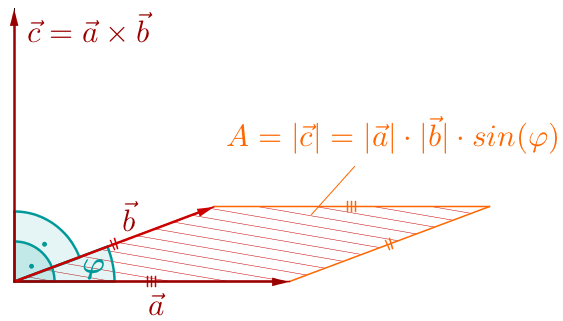
\includegraphics[width=\textwidth]{../Mathematik_1/Bilder/vektoren_kreuzprodukt_parallelogrammflaeche.png}
\end{minipage}
\begin{minipage}{0.56\textwidth}

Der Vektor \(\vec a\times\vec b\) steht senkrecht auf beiden
Ausgangsvektoren:
\[
\langle
\vec a\times\vec b,
\vec a
\rangle
=
0
\]
und
\[
\langle
\vec a\times\vec b,
\vec b
\rangle
=
0.
\]

Seine Richtung wird durch die Orientierung von
\(\vec a\) und \(\vec b\) festgelegt. Die Vektoren
\[
\vec a,\quad
\vec b,\quad
\vec a\times\vec b
\]
bilden in dieser Reihenfolge ein Rechtssystem. Die Richtung kann mit der
Rechte-Hand-Regel bestimmt werden.

\end{minipage}

Seine L�nge betr�gt
\[
\|\vec a\times\vec b\|
=
\|\vec a\|\,\|\vec b\|\sin(\varphi),
\]
wobei \(\varphi\in[0,\pi]\) der Winkel zwischen
\(\vec a\) und \(\vec b\) ist.

\end{theorembox}

Die Formel f�r die L�nge besitzt eine unmittelbare geometrische Bedeutung.
Die Vektoren \(\vec a\) und \(\vec b\) spannen ein
Parallelogramm auf. Wird \(\vec a\) als Grundseite gew�hlt, so besitzt
dieses Parallelogramm die H�he
\(\|\vec b\|\sin(\varphi)\). Sein Fl�cheninhalt ist daher
\[
A
=
\|\vec a\|\,
\|\vec b\|\sin(\varphi)
=
\|\vec a\times\vec b\|.
\]

Der Betrag des Kreuzprodukts entspricht somit dem Fl�cheninhalt des von den
beiden Vektoren aufgespannten Parallelogramms. F�r den Fl�cheninhalt des
zugeh�rigen Dreiecks gilt entsprechend
\[
A_\triangle
=
\frac12\|\vec a\times\vec b\|.
\]

\begin{defbox}{Berechnung des Kreuzprodukts}{ }

F�r
\[
\vec a
=
\begin{pmatrix}
a_1\\a_2\\a_3
\end{pmatrix},
\qquad
\vec b
=
\begin{pmatrix}
b_1\\b_2\\b_3
\end{pmatrix}
\]
ist das Kreuzprodukt definiert durch
\[
\vec a\times\vec b
=
\begin{pmatrix}
a_2\cdot b_3-a_3\cdot b_2\\
a_3\cdot b_1-a_1\cdot b_3\\
a_1\cdot b_2-a_2\cdot b_1
\end{pmatrix}.
\]

\end{defbox}

Die Reihenfolge der beiden Vektoren ist wesentlich. Beim Vertauschen der
Faktoren �ndert sich die Orientierung und damit das Vorzeichen:
\[
\vec b\times\vec a
=
-\vec a\times\vec b.
\]
Das Kreuzprodukt ist also nicht kommutativ.

\begin{exabox}{Kreuzprodukt zweier Vektoren}{ }

Gegeben seien
\[
\vec a
=
\begin{pmatrix}
3\\4\\5
\end{pmatrix},
\qquad
\vec b
=
\begin{pmatrix}
2\\-3\\1
\end{pmatrix}.
\]

Das Kreuzprodukt ergibt sich zu
\[
\begin{aligned}
\vec a\times\vec b
&=
\begin{pmatrix}
4\cdot1-5\cdot(-3)\\
5\cdot2-3\cdot1\\
3\cdot(-3)-4\cdot2
\end{pmatrix}\\[1ex]
&=
\begin{pmatrix}
19\\7\\-17
\end{pmatrix}.
\end{aligned}
\]

Die geometrische Bedeutung kann unmittelbar mithilfe des Skalarprodukts
�berpr�ft werden. F�r den ersten Ausgangsvektor gilt
\[
\begin{aligned}
\left\langle
\begin{pmatrix}3\\4\\5\end{pmatrix},
\begin{pmatrix}19\\7\\-17\end{pmatrix}
\right\rangle
&=
3\cdot19+4\cdot7+5\cdot(-17)\\
&=
57+28-85\\
&=
0.
\end{aligned}
\]

F�r den zweiten Ausgangsvektor ergibt sich entsprechend
\[
\begin{aligned}
\left\langle
\begin{pmatrix}2\\-3\\1\end{pmatrix},
\begin{pmatrix}19\\7\\-17\end{pmatrix}
\right\rangle
&=
2\cdot19-3\cdot7-17\\
&=
38-21-17\\
&=
0.
\end{aligned}
\]

Der berechnete Vektor steht somit tats�chlich senkrecht auf
\(\vec a\) und auf \(\vec b\).

Seine L�nge ist
\[
\|\vec a\times\vec b\|
=
\sqrt{19^2+7^2+(-17)^2}
=
\sqrt{699}.
\]
Damit betr�gt auch der Fl�cheninhalt des von
\(\vec a\) und \(\vec b\) aufgespannten Parallelogramms
\(\sqrt{699}\).

\end{exabox}


\subsubsection*{Typische Anwendungen des Kreuzprodukts}

Die geometrischen Eigenschaften des Kreuzprodukts f�hren unmittelbar zu
mehreren wichtigen Anwendungen.

Soll zu zwei nicht parallelen Vektoren
\(\vec a,\vec b\in\mathbb R^3\) eine Richtung bestimmt werden,
die auf beiden senkrecht steht, liefert
\[
\vec c
=
\vec a\times\vec b
\]
eine solche Richtung.

Auch Parallelit�t kann mithilfe des Kreuzprodukts gepr�ft werden. F�r zwei
Vektoren gilt
\[
\vec a\parallel\vec b
\quad\Longleftrightarrow\quad
\vec a\times\vec b=\vec 0.
\]
Denn bei parallelen oder antiparallelen Vektoren ist der eingeschlossene
Winkel \(0\) beziehungsweise \(\pi\), sodass
\(\sin(\varphi)=0\) und damit
\(\|\vec a\times\vec b\|=0\).

Schlie�lich liefert die L�nge des Kreuzprodukts den Fl�cheninhalt des aufgespannten Parallelogramms. 
 \newpage % Ebene und Raum Grundlagen
\setcounter{exercise}{0} 
\ifintegriereaufgaben
\section*{Vektoren Aufgaben}\label{MA1-vektoren-aufgaben}

	Regeln und Beispiele, die zur Bearbeitung der Aufgaben hilfreich sind, finden Sie im Skript\wennreferenzvorhanden{MA1-vektoren}{ (Abschnitt \abschnittsverweis{MA1-vektoren})} und, falls Sie nicht weiterkommen, schauen Sie \hyperref[MA1-vektoren-loesungen]{hier}.
\else
\section{Vektoren Aufgaben}\label{MA1-vektoren-aufgaben}

	Regeln und Beispiele, die zur Bearbeitung der Aufgaben hilfreich sind, finden Sie im Skript und, falls Sie nicht weiterkommen, schauen Sie \hyperref[MA1-vektoren-loesungen]{hier}.
\fi 

\begin{exercisebox}[Rechenregeln]
	Gegeben seien die Vektoren 
	\[ \boldsymbol a = \left( \begin{array}{c} -4 \\ 3 \end{array}\right)\,, \;  
		\boldsymbol b = \left( \begin{array}{c} 0 \\ -3 \end{array}\right)\,,  \;
	\boldsymbol c = \left( \begin{array}{c} -2 \\ -2 \end{array}\right)\,. \] 
	\begin{itemize}
		\item[(a)] Berechnen Sie folgende Ausdr�cke: 
			\( -\boldsymbol a + 3\cdot \boldsymbol b, \quad (2\cdot \boldsymbol a - \boldsymbol b) + 3\cdot \boldsymbol c, \quad (3\cdot \boldsymbol c - \boldsymbol b) + 2\cdot \boldsymbol a \)
		\item[(b)] Berechnen Sie die folgenden Betr�ge (L�ngen, Normen): 
			\( |\boldsymbol a|\,,\quad |\boldsymbol b|\,,\quad |\boldsymbol a+ \boldsymbol b|\,,\quad |-\boldsymbol a+3\cdot \boldsymbol b| \)
		\item[(c)] Bestimmen Sie einen Vektor der L�nge $10$, der in die gleiche Richtung wie der Gegenvektor von $\boldsymbol a$ zeigt. 
		\item[(d)] Berechnen Sie die folgenden Ausdr�cke:
			\( \boldsymbol a\boldsymbol \cdot \boldsymbol b, \quad 
			\boldsymbol a\boldsymbol \cdot \boldsymbol c, \quad 
			\boldsymbol a\boldsymbol \cdot ( 4\cdot \boldsymbol c), \quad 
			\boldsymbol a\boldsymbol \cdot ( \boldsymbol b\boldsymbol \cdot \boldsymbol c), \quad 
		(\boldsymbol a\boldsymbol \cdot  \boldsymbol b)\boldsymbol \cdot \boldsymbol c \)
	\item[(e)] Bestimmen Sie die Winkel im Bogenma� zwischen folgenden Vektoren \( \boldsymbol a\; \textnormal{und}\; \boldsymbol b, \quad \boldsymbol a \; \textnormal{und}\; \boldsymbol c\,.\)
		\item[(f)] Bestimmen Sie alle orthogonalen Vektoren zu $\boldsymbol a$.
		\item[(g)] Bestimmen Sie einen Vektor der Form $\boldsymbol b+\lambda\cdot \boldsymbol c$ mit $\lambda \in \mathbb R$, der senkrecht zu $\boldsymbol a$ ist.
		\item[(h)] Bestimmen Sie die orthogonale Zerlegung von $\boldsymbol b$ bzgl. $\boldsymbol a$, das hei�t die Vektoren $\boldsymbol b_\parallel$ und $\boldsymbol b_\perp$.
	\end{itemize}
\end{exercisebox}

\begin{exercisebox}[Rechenregeln]
	Gegeben sind die Vektoren \[ \boldsymbol a = \left( \begin{array}{c} -2 \\ 0 \\ -4\end{array}\right), \quad \boldsymbol b = \left( \begin{array}{c} -2 \\1 \\ -2 \end{array}\right), \quad \boldsymbol c = \left( \begin{array}{c} -1 \\ 1 \\0 \end{array}\right) \,. 
	\]
		\begin{itemize}
			\item[(a)] Berechnen Sie $-3\cdot(-2\cdot \boldsymbol a + \boldsymbol b) - \boldsymbol c$.
			\item[(b)] Berechnen Sie die folgenden Betr�ge (L�ngen, Normen): $|\boldsymbol a|, |\boldsymbol b|, |-3\cdot(-2\cdot \boldsymbol a + \boldsymbol b) - \boldsymbol c|$.
			\item[(c)] Berechnen Sie den Einheitsvektor in Richtung $\boldsymbol a$.
			\item[(d)] Berechnen Sie $\boldsymbol a\boldsymbol \cdot \boldsymbol b$ und $(-3\cdot \boldsymbol a)\boldsymbol \cdot \boldsymbol b$.
			\item[(e)] Berechenn Sie den Winkel $\varphi$ im Bogenma� zwischen $\boldsymbol a$ und $\boldsymbol b$ (Skalarprodukt!).
			\item[(f)] Berechnen Sie $\boldsymbol a\times \boldsymbol b$ und $\boldsymbol c\times (\boldsymbol a\times \boldsymbol b)$.
			%\item[(g)] Pr�fen Sie anhand der definierten Vektoren, dass gilt \[ \boldsymbol c\times ( \boldsymbol a\times \boldsymbol b) = (\boldsymbol c\boldsymbol \cdot \boldsymbol b)\boldsymbol \cdot \boldsymbol a -(\boldsymbol c\boldsymbol \cdot \boldsymbol a)\boldsymbol \cdot \boldsymbol b\] 
			\item[(g)] Berechnen Sie die Fl�che des durch $\boldsymbol a$ und $\boldsymbol b$ aufgespannten Parallelogramms. 
\end{itemize}
\end{exercisebox}

\begin{exercisebox}[Rechenregeln]
	Gegeben sind die folgenden Vektoren
	\[ \boldsymbol a = \left( \begin{array}{c} 1+2i \\ -i \\ 0 \\3 \end{array}\right), \quad \boldsymbol b = \left( \begin{array}{c} -3-i \\ 2i \\ 0 \\ -i\end{array}\right), \quad 
	\boldsymbol c = \left( \begin{array}{c} -2+i \\ 1+2i \end{array}\right), \quad \boldsymbol d = \left( \begin{array}{c} -i \\ -1-3i\end{array}\right)  \,. \]
	\begin{itemize}
		\item[(a)] Berechnen Sie $-i\boldsymbol a + (2-i)\boldsymbol b$.
		\item[(b)] Berechnen Sie $\langle \boldsymbol a, \boldsymbol b\rangle$.
		\item[(c)] Berechnen Sie $|\boldsymbol a|$.
		\item[(d)] Berechnen Sie die folgenden Ausdr�cke: \( |\boldsymbol c|, \quad \langle \boldsymbol c, \boldsymbol d\rangle, \quad \langle \boldsymbol d, \boldsymbol c\rangle\)
		\item[(e)] Bestimmen Sie eine Zerlegung von $\boldsymbol d$ der folgenden Art \( \boldsymbol d = \boldsymbol d_\perp + \boldsymbol d_\parallel, \quad \boldsymbol d_\perp \perp \boldsymbol c\,.\)
	\end{itemize}
\end{exercisebox}

%\begin{theorembox}[Linearkombination]
%  Ein Vektor $\boldsymbol x\in \mathbb R^n$ der Form
%  \begin{eqnarray*}
%    \boldsymbol x = \alpha_1 \boldsymbol x_1 + \alpha_2 \boldsymbol x_2 + \dots + \alpha_m\boldsymbol x_m, \quad \alpha_i \in \mathbb R, \boldsymbol x_i\in \mathbb R^n, \; i=1,\dots, m\,, 
%  \end{eqnarray*}
%  hei�t Linearkombination der Vektoren $\boldsymbol x_1, \dots, \boldsymbol x_m$.
%\end{theorembox}
%
%\begin{theorembox}[Lineare Unabh�ngigkeit, lineare Abh�ngigkeit]
%  Ein Vektorsystem $(\boldsymbol x_1, \boldsymbol x_2, \dots, \boldsymbol x_m)$ ($m$-Tupel) hei�t linear unabh�ngig, wenn gilt
%  \begin{eqnarray*}
%    \sum\limits_{i=1}^m \alpha_i\boldsymbol x_i = \boldsymbol 0 \Rightarrow  \forall i=1,\dots, m: \; \alpha_i = 0\,,
%  \end{eqnarray*}
%  andernfalls hei�en die Vektoren linear abh�ngig.
%\end{theorembox}
%
%\begin{theorembox}[Lineare Abh�ngigkeit]
%Merke: Sind die Vektoren $\boldsymbol x_1, \dots, \boldsymbol x_m\in \mathbb R^n$ linear abh�ngig, so kann man mindestens einen der Vektoren als lineare Kombination der anderen darstellen.
%\end{theorembox}
%
%\begin{theorembox}[Skalarprodukt]
%  Sei $\boldsymbol v =(v_1,\dots,v_n)^\intercal, \boldsymbol u =(u_1,\dots,u_n)^\intercal \in \mathbb R^n$. Das Skalarprodukt $\langle \boldsymbol u, \boldsymbol v\rangle$ ist definiert als  
%  
%  \begin{eqnarray*}
%    \langle \boldsymbol u, \boldsymbol v\rangle :=   \sum\limits_{i=1}^n v_i u_i = v_1 u_1+v_2 u_2 + \dots + v_n u_n\in \mathbb R\,.
%\end{eqnarray*}
%\end{theorembox}

%\begin{exercisebox}[Skalarprodukt in $\mathbb R^n$]
%  Ist die folgende Aussage wahr oder falsch? "Das Skalarprodukt ist keine Multiplikation von Vektoren."
%\end{exercisebox}

%\begin{exercisebox}[Kosinussatz]
%	Betrachten Sie ein Dreieck mit den Kantenvektoren $\boldsymbol a, \boldsymbol b$ und Winkel $\alpha$ und zeigen Sie:
%	\[c^2 = a^2 + b^2 - 2\, a\, b \, \cos(\alpha)\,.\]
%\end{exercisebox}
%\begin{exercisebox}[Satz des Thales]
%	Jeder Winkel im Halbkreis ist ein rechter Winkel. 
%\end{exercisebox}
%
%\begin{exercisebox}[Kreuzprodukt] 
%	Zeigen Sie allgemein, dass f�r $\boldsymbol u, \boldsymbol v\in \mathbb R^3$ der Vektor $\boldsymbol v$ senkrecht auf $\boldsymbol u \times \boldsymbol v$ steht. 
%\end{exercisebox}

%\begin{exercisebox}[Skalarprodukt]
%  Skalarpodukt als Projektion.
%\end{exercisebox}

%\begin{exercisebox}[Anwendung Kreuzprodukt]
%	\begin{itemize}
%		\item Mechanik: Drehimpuls 
%		\item Elektrotechnik: Maxwell Gleichungen
%	\end{itemize}
%\end{exercisebox}

%\begin{exercisebox}[ Mercator Projektion]
%\end{exercisebox}
%
%\begin{exercisebox}[Differentialgeometrie]
%	\begin{itemize}
%		\item Gau�sche Kr�mmung, Mittlere Kr�mmung,
%		\item Isometrie
%		\item Isomorphismen (Problem Kugel)
%	\end{itemize}
%\end{exercisebox}
%
%\begin{exercisebox}[Relativit�tstheorie]
%	Kr�mmung der Raumzeit, Ursprung der Gravitationskraft
%\end{exercisebox}
%
%\begin{exercisebox}[$\mathbb R^n$]
%  $V=\mathbb R^n$ ist ein Vektorraum �ber dem K�rper $G = \mathbb R$.
%\end{exercisebox}

%\begin{exercisebox}[Metrik]
%	Vektorraum
%\end{exercisebox}
 \newpage 
\setcounter{satz}{0} \setcounter{def}{0} \setcounter{exa}{0}  \section{Vektorraum}\label{MA1-vektorraum}

\begin{table}[H]
  \centering
  \begin{tabularx}{\textwidth}{p{0.9\textwidth} p{0.1\textwidth}}
    \toprule
	  \multicolumn{2}{c}{\textbf{�bersicht �ber Lernziele und Voraussetzungen}}\\
    \midrule
\textbf{Lernziele} &\\[.5\normalbaselineskip]
\tabitem den Begriff des Vektorraums erkl�ren und Beispiele f�r Vektorr�ume
�ber \(\mathbb R\) und \(\mathbb C\) einordnen &\\
\tabitem Linearkombinationen von Vektoren bilden und Erzeugendensysteme
interpretieren &\\
\tabitem lineare Unabh�ngigkeit und lineare Abh�ngigkeit erkl�ren und
anhand einfacher Beispiele interpretieren &\\
\tabitem die Begriffe Basis und Dimension eines Vektorraums erkl�ren und
ihren Zusammenhang beschreiben &\\
\tabitem Geraden durch den Ursprung als eindimensionale Untervektorr�ume
interpretieren (+) &\\[.5\normalbaselineskip]
    \midrule
      \textbf{Voraussetzungen} &\\[.5\normalbaselineskip]
      \tabitem Vektoren in $\mathbb R^n$ (Addition und Skalierung, Skalarprodukt) & \abschnittsverweis{MA1-vektoren}\\
    \bottomrule
  \end{tabularx}
\end{table}

\ifintegriereaufgaben \noindent �bungsaufgaben zum Thema finden Sie hier: \hyperref[MA1-vektorraum-aufgaben]{Aufgaben}
\vspace{0.3cm}
\hrule
\fi

\subsection{Was ist ein Vektorraum?}

Im vorangegangenen Abschnitt wurden zun�chst Vektoren in \(\mathbb R^n\) und \(\mathbb C^n\) betrachtet. Zwei Vektoren desselben Raumes k�nnen addiert werden, und ein Vektor kann mit einem Skalar multipliziert werden. Dabei entsteht jeweils wieder ein Vektor desselben Raumes.

Diese beiden Operationen besitzen au�erdem eine Reihe vertrauter Recheneigenschaften. Die Vektoraddition ist beispielsweise assoziativ und kommutativ. Es gibt einen Nullvektor, und zu jedem Vektor existiert ein Gegenvektor. Auch die Skalarmultiplikation vertr�gt sich in bestimmter Weise mit der Addition.

Entscheidend ist nun, dass diese Eigenschaften nicht an Spalten aus reellen oder komplexen Zahlen gebunden sind. Immer wenn eine Menge von Objekten mit einer Addition und einer Skalarmultiplikation ausgestattet ist und dieselben grundlegenden Rechengesetze erf�llt, entsteht dieselbe algebraische Struktur.

Diese Struktur hei�t \textbf{Vektorraum} (\emph{vector space}). Die Elemente eines Vektorraums hei�en \textbf{Vektoren} (\emph{vectors}), unabh�ngig davon, ob sie geometrisch als Pfeile dargestellt werden k�nnen.

\begin{defbox}{Vektorraum}{ }

Es sei \(\mathbb K\) ein K�rper, hier insbesondere
\(\mathbb K=\mathbb R\) oder \(\mathbb K=\mathbb C\).
Eine nichtleere Menge \(\mathbb V\) hei�t
\textbf{Vektorraum} (\emph{vector space}) �ber \(\mathbb K\), wenn auf
\(\mathbb V\)

eine Vektoraddition
\[
+:\mathbb V\times\mathbb V\to\mathbb V,
\qquad
(\vec u,\vec v)\mapsto
\vec u+\vec v,
\]
und eine Skalarmultiplikation
\[
\cdot:\mathbb K\times\mathbb V\to\mathbb V,
\qquad
(\lambda,\vec v)\mapsto\lambda\cdot \vec v
\]
definiert sind und f�r alle
\(\vec u,\vec v,\vec w\in\mathbb V\) sowie
\(\lambda,\mu\in\mathbb K\) die folgenden Rechengesetze gelten:

\begin{enumerate}
    \item
    \(\vec u+\vec v
    =\vec v+\vec u\),

    \item
    \((\vec u+\vec v)+\vec w
    =\vec u+(\vec v+\vec w)\),

    \item es existiert ein Nullvektor
    \(\vec 0\in\mathbb V\) mit
    \(\vec v+\vec 0=\vec v\),

    \item zu jedem \(\vec v\in\mathbb V\) existiert ein
    Gegenvektor \(-\vec v\) mit
    \(\vec v+(-\vec v)=\vec 0\),

    \item
    \(\lambda\cdot (\vec u+\vec v)
    =\lambda\cdot \vec u+\lambda\cdot \vec v\),

    \item
    \((\lambda+\mu)\cdot \vec v
    =\lambda\cdot \vec v+\mu\cdot \vec v\),

    \item
    \((\lambda\cdot \mu)\cdot \vec v
    =\lambda\cdot (\mu\cdot \vec v)\),

    \item
    \(1\cdot \vec v=\vec v\).
\end{enumerate}

\end{defbox}

Die Bezeichnung �Vektor� beschreibt damit nicht die �u�ere Form eines mathematischen Objekts, sondern seine Rolle innerhalb einer linearen Struktur. Spaltenvektoren sind wichtige Beispiele f�r Vektoren, aber nicht die einzigen.

Ein besonders wichtiges Beispiel zeigt, wie weit der Begriff des Vektors �ber geometrische Pfeile und Zahlenspalten hinausreicht.

Auch Funktionen k�nnen addiert und mit Skalaren multipliziert werden. F�r zwei Funktionen \(f,g:\mathbb R\to\mathbb R\) und \(\lambda\in\mathbb R\) werden die Operationen punktweise definiert:
\[
(f+g)(x)=f(x)+g(x)
\]
und
\[
(\lambda f)(x)=\lambda \cdot  f(x).
\]

Das Ergebnis ist jeweils wieder eine Funktion von \(\mathbb R\) nach \(\mathbb R\). Auch die �brigen Vektorraumaxiome werden von diesen Operationen erf�llt. Damit bilden beispielsweise die reellwertigen Funktionen auf \(\mathbb R\) einen Vektorraum.

\begin{exabox}{Funktionen als Vektoren}{ }

Die Funktionen
\[
f(x)=e^x
\qquad\text{und}\qquad
g(x)=\sin(x)
\]
k�nnen als Vektoren eines Funktionenraumes aufgefasst werden.

Die Skalarmultiplikation mit \(3\) liefert
\[
(3f)(x)=3e^x.
\]

Die Addition zweier Funktionen liefert beispielsweise
\[
(\sin+\cos)(x)=\sin(x)+\cos(x).
\]

Der Nullvektor dieses Vektorraums ist die \textbf{Nullfunktion}
\[
0:\mathbb R\to\mathbb R,
\qquad
x\mapsto0.
\]

Auch der Gegenvektor einer Funktion ist wieder eine Funktion:
\[
(-f)(x)=-f(x).
\]

\end{exabox}

Die Bezeichnung �Vektor� impliziert die G�ltigkeit von Operationen und die daf�r geltenden Rechengesetze. Diese Sichtweise wird sp�ter besonders wichtig: Funktionenr�ume erm�glichen, Methoden der linearen Algebra auf Funktionen zu �bertragen.

\subsection{Basis und Dimension}

Die Vektoren der Vektorr�ume $\mathbb R^3$ lassen sich entsprechend ihrer \(x,\,y\) und \(z\)-Komponenten zerlegen:
$$\left(\begin{array}{c} 5 \\ 6 \\ 3\end{array}\right) = 5\left(\begin{array}{c} 1 \\ 0 \\ 0\end{array}\right) +  6\left(\begin{array}{c} 0 \\ 1 \\ 0\end{array}\right) + 3\left(\begin{array}{c} 0 \\ 0 \\ 1\end{array}\right)\,, \quad \quad (*)$$
wobei die Vektoren auf der rechten Seite zwei besondere Eigenschaften besitzen: sie sind \textbf{orthonormal} (\emph{orthonormal}) und das hei�t
\begin{itemize}
  \item sie stehen gegenseitig senkrecht aufeinander und 
  \item sie sind alle von der L�nge eins.
\end{itemize}
Jeder Vektor des $\mathbb R^3$ l�sst sich aus diesen Einheitsvektoren zusammensetzen und die Zerlegung ist eindeutig. Man nennt die drei Einheitsvektoren die Standardbasis des $\mathbb R^3$ und weil die Standardbasis so oft vorkommt, benutzt man abk�rzende Schreibweisen. Die folgenden sind die g�ngigsten:
\begin{defbox}{Standardbasis des \(\mathbb R^3\)}{ }
	$ \left\{ \left( \begin{array}{c} 1 \\0 \\0\end{array}\right), \left( \begin{array}{c} 0 \\1 \\0\end{array}\right), \left( \begin{array}{c} 0 \\0 \\1\end{array}\right)\right\} \; \widehat = \; \left\{ \vec e_x, \, \vec e_ y, \vec e_z\right\} \; \widehat = \; \left\{ \vec e_1, \, \vec e_2, \,\vec e_3\right\}$.
%In �lteren Texten steht statt dessen $\vec i, \, \vec j, \, \vec k$. 
\end{defbox}
Entsprechende \textbf{Standardbasen} (\emph{canonical basis}) mit orthonormalen Vektoren gibt es in allen R�umen $\mathbb R^n$ und $\mathbb C^n$. 

Das Beispiel der Standardbasis zeigt ein grundlegendes Prinzip: Ein Vektor wird aus anderen Vektoren aufgebaut, indem diese mit Skalaren multipliziert und anschlie�end addiert werden. Eine solche Darstellung hei�t \textbf{Linearkombination} (\emph{linear combination}).

\begin{defbox}{Linearkombination}{ }

Es seien
\(\vec v_1,\ldots,\vec v_m\in\mathbb V\).
Jeder Vektor der Form
\[
\lambda_1\cdot \vec v_1
+\lambda_2\cdot \vec v_2
+\cdots+
\lambda_m\cdot \vec v_m,
\qquad
\lambda_1,\ldots,\lambda_m\in\mathbb K,
\]
hei�t \textbf{Linearkombination} der Vektoren
\(\vec v_1,\ldots,\vec v_m\).

\end{defbox}

Im Beispiel der Standardbasis des \(\mathbb R^3\) l�sst sich jeder Vektor als Linearkombination von \(\vec e_1,\vec e_2,\vec e_3\) darstellen. Die drei Vektoren reichen also aus, um den gesamten Raum zu erzeugen.

\begin{defbox}{Erzeugendensystem}{ }

Eine Menge von Vektoren
\(\{\vec v_1,\ldots,\vec v_m\}\subseteq\mathbb V\)
hei�t \textbf{Erzeugendensystem} (\emph{spanning set}) von
\(\mathbb V\), wenn sich jeder Vektor
\(\vec v\in\mathbb V\) als Linearkombination dieser Vektoren
darstellen l�sst.

\end{defbox}

Ein Erzeugendensystem kann allerdings mehr Vektoren enthalten als notwendig.  Damit stellt sich eine zweite Frage: Welche der erzeugenden Vektoren tragen tats�chlich neue Information bei und welche lassen sich bereits aus den anderen zusammensetzen?

Diese Frage f�hrt zur linearen Unabh�ngigkeit.

\begin{defbox}{Lineare Abh�ngigkeit und lineare Unabh�ngigkeit}{ }

Es seien
\(\vec v_1,\ldots,\vec v_m\in\mathbb V\).

Die Vektoren hei�en \textbf{linear unabh�ngig}
(\emph{linearly independent}), wenn aus
\[
\lambda_1\cdot \vec v_1+\cdots+\lambda_m\cdot \vec v_m
=
\vec 0
\]
notwendig
\[
\lambda_1=\cdots=\lambda_m=0
\]
folgt.

Existieren dagegen Skalare
\(\lambda_1,\ldots,\lambda_m\), die nicht alle null sind und trotzdem
\[
\lambda_1\cdot \vec v_1+\cdots+\lambda_m\cdot \vec v_m
=
\vec 0
\]
erf�llen, so hei�en die Vektoren \textbf{linear abh�ngig}
(\emph{linearly dependent}).

\end{defbox}

Lineare Abh�ngigkeit bedeutet anschaulich, dass mindestens einer der beteiligten Vektoren durch die anderen erzeugt werden kann. Dieser Vektor liefert dann keine zus�tzliche unabh�ngige Richtung.

Beispielsweise sind
\[
\begin{pmatrix}1\\2\end{pmatrix}
\qquad\text{und}\qquad
\begin{pmatrix}2\\4\end{pmatrix}
\]
linear abh�ngig, denn der zweite Vektor ist das Doppelte des ersten. Dagegen
sind
\[
\begin{pmatrix}1\\0\end{pmatrix}
\qquad\text{und}\qquad
\begin{pmatrix}0\\1\end{pmatrix}
\]
linear unabh�ngig.

Eine \textbf{Basis} verbindet nun die beiden zuvor eingef�hrten Eigenschaften: eine Basis ist eine Menge von Vektoren, die den gesamten Vektorraum erzeugt und gleichzeitig keine �berfl�ssigen Vektoren enth�lt.

\begin{defbox}{Basis eines Vektorraums}{ }

Eine Menge
\[
B=\{\vec v_1,\ldots,\vec v_m\}
\]
von Vektoren eines Vektorraums \(\mathbb V\) hei�t
\textbf{Basis} (\emph{basis}) von \(\mathbb V\), wenn

\begin{itemize}
    \item die Vektoren
    \(\vec v_1,\ldots,\vec v_m\)
    linear unabh�ngig sind und

    \item
    \(\vec v_1,\ldots,\vec v_m\)
    ein Erzeugendensystem von \(\mathbb V\) bilden.
\end{itemize}

Damit l�sst sich jeder Vektor \(\vec v\in\mathbb V\) eindeutig in der
Form
\[
\vec v
=
\lambda_1\cdot \vec v_1+\cdots+\lambda_m\cdot \vec v_m,
\qquad
\lambda_1,\ldots,\lambda_m\in\mathbb K,
\]
darstellen.

\end{defbox}

Die beiden Bedingungen einer Basis erf�llen unterschiedliche Aufgaben. Das Erzeugendensystem stellt sicher, dass jeder Vektor des Raumes dargestellt werden kann. Die lineare Unabh�ngigkeit stellt sicher, dass diese Darstellung eindeutig ist.

Die Skalare \(\lambda_1,\ldots,\lambda_m\) hei�en die \textbf{Koordinaten} von \(\vec v\) bez�glich der gew�hlten Basis.


\noindent\textbf{Bemerkungen:}\marginpar{\small Aufgaben}
\begin{itemize}
	\item Eine Basis eines Vektorraums ist nicht eindeutig und manchmal ist es sogar sinnvoll, mit einer nicht orthogonalen Basis zu rechnen anstatt mit einer Orthonormalbasis. 
	\item Eine Basis ist ein bez�glich der Aufnahme weiterer Vektoren maximales linear unabh�ngiges System. Gleichwertig kann eine Basis als ein Erzeugendensystem aufgefasst werden, aus dem kein Vektor entfernt werden kann, ohne die Erzeugendeneigenschaft zu verlieren.
	\item Die Anzahl der Basisvektoren eines Vektorraums nennt man \textbf{Dimension} (\emph{dimension}) des Vektorraums.
\end{itemize}

\begin{exabox}{Dimension von Vektorr�umen}{ }
  \begin{itemize}
    \item Der Raum $\mathbb R^{17}$ hat die  Dimension $17$: $\mathrm{dim}\left( \mathbb R^{17}\right) = 17$,
    \item Der Raum der stetigen Funktionen von $\mathbb R$ nach $\mathbb R$ ist unendlichdimensional.
  \end{itemize}
\end{exabox}

\subsubsection*{Geraden durch den Ursprung als eindimensionale Untervektorr�ume}

Der Begriff der Dimension erh�lt bereits bei Geraden eine anschauliche Bedeutung. Dazu sei ein von Null verschiedener Vektor
\(\vec v\in\mathbb R^3\) gegeben. Alle skalaren Vielfachen dieses Vektors bilden die Menge
\[
U
=
\left\{
\lambda\cdot \vec v:
\lambda\in\mathbb R
\right\}.
\]

Geometrisch beschreibt diese Menge eine Gerade durch den Ursprung mit Richtung \(\vec v\).

F�r
\[
\vec v
=
\begin{pmatrix}
2\\
2\\
-1
\end{pmatrix}
\]
ergibt sich beispielsweise
\[
U
=
\left\{
\lambda\cdot 
\begin{pmatrix}
2\\
2\\
-1
\end{pmatrix}
:
\lambda\in\mathbb R
\right\}.
\]

Die Menge \(U\) ist nicht nur eine Gerade, sondern zugleich selbst ein Vektorraum. Dies l�sst sich unmittelbar anhand der Vektorraumoperationen erkennen.

Zun�chst geh�rt der Nullvektor zu \(U\), denn f�r \(\lambda=0\) gilt
\[
0\cdot \vec v=\vec 0.
\]

Werden zwei beliebige Vektoren aus \(U\) addiert, so entsteht wieder ein Vektor aus \(U\). F�r
\(\lambda\cdot \vec v,\mu\cdot\vec v\in U\) gilt
\[
\lambda\cdot \vec v+\mu\cdot \vec v
=
(\lambda+\mu)\cdot \vec v
\in U.
\]

Auch die Multiplikation eines Vektors aus \(U\) mit einem beliebigen Skalar
f�hrt nicht aus \(U\) heraus. F�r \(c\in\mathbb R\) gilt
\[
c\cdot (\lambda\cdot \vec v)
=
(c\cdot \lambda)\cdot \vec v
\in U.
\]

Die Menge ist damit bez�glich Vektoraddition und Skalarmultiplikation abgeschlossen. Da die �brigen Vektorraumaxiome von \(\mathbb R^3\) �bernommen werden, bildet \(U\) selbst einen Vektorraum.

Ein Vektorraum, der als Teilmenge eines gr��eren Vektorraums auftritt und dessen Vektorraumoperationen �bernimmt, hei�t \textbf{Untervektorraum} (\emph{vector subspace}).

\begin{defbox}{Untervektorraum}{ }

Eine nichtleere Teilmenge \(U\subseteq\mathbb V\) eines Vektorraums
\(\mathbb V\) hei�t Untervektorraum, wenn f�r alle
\(\vec u,\vec v\in U\) und alle
\(\lambda\in\mathbb K\) gilt:
\[
\vec u+\vec v\in U
\qquad\text{und}\qquad
\lambda\cdot \vec u\in U.
\]

\end{defbox}

\noindent\textbf{Bemerkung:}
Jeder Untervektorraum enth�lt notwendigerweise den Nullvektor. Ist
\(\vec u\in U\), so folgt aus der Abgeschlossenheit bez�glich der
Skalarmultiplikation
\[
0\cdot\vec u=\vec 0\in U.
\]
Fehlt der Nullvektor in einer gegebenen Teilmenge, kann diese daher kein
Untervektorraum sein.

F�r die Gerade
\[
U
=
\{\lambda\cdot \vec v:\lambda\in\mathbb R\}
\]
reicht ein einziger von Null verschiedener Vektor aus, um jeden Vektor des
Raumes \(U\) darzustellen. Die Menge
\[
\{\vec v\}
\]
ist daher eine Basis von \(U\), und es gilt
\[
\dim(U)=1.
\]

Damit erh�lt die Bezeichnung �eindimensional� eine geometrische Interpretation: Die Geraden durch den Ursprung sind genau die eindimensionalen Untervektorr�ume von \(\mathbb R^3\).

\subsubsection*{Denkaufgabe: Muss jede Gerade ein Untervektorraum sein?}

Die Gerade \[ g = \left\{ \begin{pmatrix} 2\\1\\2 \end{pmatrix} + \lambda\cdot \begin{pmatrix} 2\\2\\-1 \end{pmatrix} : \lambda\in\mathbb R \right\} \] besitzt dieselbe Richtung wie ein eindimensionaler Untervektorraum, ist jedoch gegen�ber dem Ursprung verschoben. \begin{exabox}{Denkaufgabe}{ } Ist die Gerade \(g\) ein Untervektorraum von \(\mathbb R^3\)? Welche Eigenschaft eines Untervektorraums kann besonders einfach �berpr�ft werden, um diese Frage zu entscheiden? \end{exabox}

\subsubsection*{Zusammenfassung}

Kennt man eine Basis des Vektorraums, dann kennt man quasi alles andere - die Basisvektoren stehen stellvertretend f�r alle Vektoren des Vektorraums. Damit wird klar: die Analyse eines Vektorraums ist eng verkn�pft mit der Analyse linearer Unabh�ngigkeit von Vektoren. Und das wirft Fragen auf, beispielsweise die folgenden
\begin{itemize}
	\item Wie wird �berpr�ft, ob eine gegebene Menge von Vektoren linear unabh�ngig ist?
	\item Wie wird �berpr�ft, welche Dimension ein gegebener Vektorraum hat?
	\item Wie wird eine Basis konstruiert bzw. vervollst�ndigt? 
	\item Gibt es eine systematische Art eine Orthonormalbasis aus linear unabh�ngigen Vektoren zu konstruieren?
\end{itemize}
Diese Fragen lassen sich am einfachsten beantworten, wenn wir Werkzeuge aus der linearen Algebra nutzen, n�mlich
\begin{itemize}
	\item Bestimmung des Rangs und des Defekts einer Matrix
	\item Bestimmung des Bilds einer Matrix
	\item Bestimmung der Determinante einer Matrix
\end{itemize}
\wennreferenzvorhanden{MA1-matrizen}{\wennreferenzvorhanden{MA1-determinante-und-inverse}{Die Abschnitte \abschnittsverweis{MA1-matrizen}--\abschnittsverweis{MA1-determinante-und-inverse} f�hren diese Werkzeuge ein.}}
 \newpage % Vektorraum Grundlagen 
\setcounter{exercise}{0} \ifintegriereaufgaben
\section*{Vektorr�ume Aufgaben}\label{MA1-vektorraum-aufgaben}

	Regeln und Beispiele, die zur Bearbeitung der Aufgaben hilfreich sind, finden Sie im Skript\wennreferenzvorhanden{MA1-vektorraum}{ (Abschnitt \abschnittsverweis{MA1-vektorraum})} und, falls Sie nicht weiterkommen, schauen Sie \hyperref[MA1-vektorraum-loesungen]{hier}.
\else
\section{Vektorr�ume Aufgaben}\label{MA1-vektorraum-aufgaben}
	Regeln und Beispiele, die zur Bearbeitung der Aufgaben hilfreich sind, finden Sie im Skript und, falls Sie nicht weiterkommen, schauen Sie \hyperref[MA1-vektorraum-loesungen]{hier}.
\fi 

\begin{exercisebox}[K�rperaxiome]
  Ist die folgende Aussage wahr oder falsch? 
  \begin{center} "\,Das Skalarprodukt ist eine Multiplikation von Vektoren."\end{center}
\end{exercisebox}

\begin{exercisebox}[Vektorraum]
	Pr�fen Sie, ob die folgenden Mengen Vektorr�ume �ber \(\mathbb R\) sind oder nicht und geben Sie ggf die Dimension und eine Basis an. 
	\begin{itemize}
		\item[(a)] \( M = \{ \left(  a,\; 0, \;b\right)^\intercal,\; a, b\in\mathbb R\} \)
		\item[(b)] \( M = \{ \left( x, \; y,\right)^\intercal:\; 2x-3y = 0,\; x,y\in\mathbb R\} \)
		\item[(c)] \( M = \{ \left( a, \; a^2\right)^\intercal,\; a\in\mathbb R\} \)
	\end{itemize}
\end{exercisebox}

\begin{exercisebox}[Vektorraum]
	Es seien $\boldsymbol p$ und $\boldsymbol n$ Vektoren des $\mathbb R^3$ und \(\boldsymbol n\not=\boldsymbol 0\). 
	\begin{itemize}
		\item[(a)] Welches geometrische Objekt stellt die L�sungsmenge \(E\) der folgenden Gleichung(en) dar? 
	\[ \boldsymbol x \in \mathbb R^3: \; \langle \left( \boldsymbol x - \boldsymbol p \right), \boldsymbol n\rangle = 0\]
\item[(b)] Ist \(E\) ein reeller Vektorraum? Falls ja, geben Sie die Dimension und eine Basis an.
	\end{itemize}
\end{exercisebox}

\begin{exercisebox}[Basis]
	Gegeben sei der Vektor \( \boldsymbol a^\intercal = \left( \sqrt{3}, 1\right)^\intercal\). Bestimmen Sie zwei Vektoren \(\boldsymbol  v\) und \(\boldsymbol w\), die eine Orthonormalbasis des \(\mathbb R^2\) sind, wobei \(\boldsymbol v\) parallel zu \(\boldsymbol a\) sein soll, also \(\boldsymbol v \parallel \boldsymbol a\).
\end{exercisebox}

\begin{exercisebox}[Dimension]
	Welche Dimension haben die folgenden reellen Vektorr�ume?
	\begin{itemize}
		\item[(a)] $ \mathbb V_1 = \left\{ \boldsymbol x \in \mathbb R^n: \boldsymbol x = \alpha \boldsymbol a\,, \; \boldsymbol a \in \mathbb R^n\setminus\{\boldsymbol 0\} \right\} $
		\item[(b)] $ \mathbb V_2 = \left\{ \boldsymbol x \in \mathbb R^3: \boldsymbol x = \alpha \boldsymbol a + \beta \boldsymbol b\,, \; \boldsymbol b,\boldsymbol a \in \mathbb R^3\setminus\{ \boldsymbol 0 \}, \; \boldsymbol a \times \boldsymbol b =\boldsymbol 0 \right\}$
	\end{itemize}
\end{exercisebox}

\begin{exercisebox}[Anwendung: Krummlinige Koordinaten]
	\begin{itemize}
		\item[(a)] Bestimmen Sie die Polarkoordinaten eines beliebigen Vektors \(\boldsymbol x \in \mathbb R^2\setminus \{\boldsymbol 0\}\).
		\item[(b)] Zeigen Sie, dass  die Vektoren \[ \boldsymbol e_{\varphi} = \left( \begin{array}{c} -\sin(\varphi) \\\cos(\varphi) \end{array}\right), \; \boldsymbol e_{r} = \left( \begin{array}{c} \cos(\varphi) \\\sin(\varphi) \end{array}\right)\; \textnormal{mit}\; r\in [0,\infty), \; \varphi\in (-\frac{\pi}{2}, \frac{\pi}{2}] \] eine Orthonormalbasis des \(\mathbb R^2\) sind.
			\item[(c)] Skizzieren Sie f�r \(r=1\) und \(\varphi = \pi/4\) die Orthonormalbasen \( \{\boldsymbol e_x, \boldsymbol e_y\}  \) und \( \{\boldsymbol e_r, \boldsymbol e_\varphi\}  \) in einem gemeinsamen Koordinatensystem.  
	\end{itemize}
\end{exercisebox}
\begin{exercisebox}[Analytische Geometrie]
	Es sei $\boldsymbol r, \boldsymbol n\in\mathbb R^3$. Welches geometrische Objekt stellt die L�sungsmenge der folgenden Gleichung(en) dar? 
	\[ \boldsymbol x \in \mathbb R^3: \; \left( \boldsymbol x - \boldsymbol r \right) \boldsymbol \cdot \boldsymbol n = 0\]
\end{exercisebox}

\begin{exercisebox}[Lineare Funktion]
	Wie l��t sich eine Funktion $f:\mathbb R^n \to \mathbb R$ beschreiben, die in jedem Argument linear ist? Es gelte also \[ f( x_1, x_2, \dots, \alpha x_i, \dots, x_n) = \alpha f(x_1,x_2,\dots, x_i, \dots, x_n)\quad i=1,\dots,n\,.\]
\end{exercisebox}

\begin{theorembox}{}{Tangente und Normale}
	Es sei eine differenzierbare Funktion $f: \mathbb R \to \mathbb R$ gegeben. 
	\begin{enumerate}	
		\item Eine Gerade $g$, die an der Stelle $x_0$ denselben Funktionswert wie $f$ und dieselbe Steigung wie $f$ aufweist, nennt man Tangente an der Stelle $x_0$. Die Geradengleichung lautet \[ g: \mathbb R \to \mathbb R,\; x\mapsto f'(x_0) (x-x_0) + f(x_0)\,.\]
		\item Eine Gerade $n$, die an der Stelle $x_0$ denselben Funktionswert wie $f$ und die negative Steigung wie $f$ aufweist, nennt man Normale an der Stelle $x_0$. Die Geradengleichung lautet \[ n: \mathbb R \to \mathbb R,\; x\mapsto -f'(x_0) (x-x_0) + f(x_0)\,.\]
	\end{enumerate}
\end{theorembox}

\begin{exercisebox}[Tangenten]
	Gegeben ist die Funktion $f: \mathbb R \to \mathbb R, \; x\mapsto \frac14 x^2$. Ihr Graph sei $K$. 
  \begin{enumerate}
    \item Zeigen Sie, dass die Tangenten an $K$ in den Punkten $B_1\left(-3|\frac94\right)$ und  $B_2\left(\frac43|\frac49\right)$ orthogonal zueinander sind. Zeichnen Sie $K$ zusammen mit diesen Tangenten. 
    \item Es seien $S_1\left(a|f(a)\right)$ und  $S_2\left(b|f(b)\right)$ Punkte auf $K$. Welche Beziehung besteht zwischen $a$ und $b$, wenn die Tangenten an $K$ in $S_1$ und $S_2$ orthogonal sind?
    \item Bestimmen Sie die Punkte  $S_1\left(a|f(a)\right)$ und  $S_2\left(b|f(b)\right)$ so, dass die Tangenten in $S_1$ und $S_2$ orthogonal zueinander sind und die Strecke $S_1S_2$ parallel zur $x$-Achse ist. 
  \end{enumerate}
\end{exercisebox}

\begin{exercisebox}[Tangenten]
  \begin{enumerate}
	  \item Gegeben ist die Funktion \[ f: \mathbb R \to \mathbb R, x \mapsto \frac14 x^2 + cx\,.\] 
		  Der Graph von $f$ schneidet die $x$-Achse im Ursprung $O(0|0)$ und im Punkt $A(a|0)$. Die Tangenten an den Graphen in $O$ und $A$ schneiden sich im Punkt $B$. Zeigen Sie, dass das Dreieck $OAB$ stets gleichschenklig ist. Bestimmen Sie den Koeffizienten $c$ so, dass das Dreieck $OAB$ auch rechtwinklig ist.
	  \item Gegeben ist die Funktion \[ g: \mathbb R \to \mathbb R, \; x \mapsto 2 \sin(cx), \quad c \in (0,\infty)\,. \] Der Graph von $g$ schneidet die $x$-Achse im Ursprung $O=(0|0)$ und im Punkt $A(\frac{\pi}{c}|0)$. Die Tangenten an den Graphen in $O$ und $A$ schneiden sich im Punkt $B$. Bestimmen Sie den Koeffizienten $c$ so, dass das Dreieck $OAB$ gleichseitig ist. 
  \end{enumerate}
\end{exercisebox}

%\begin{exercisebox}[Mathematik lesen]
%	$\forall \boldsymbol u, \boldsymbol v\mathbb R^n: \quad |\boldsymbol u \boldsymbol \cdot \boldsymbol v| \leq |\boldsymbol u| \cdot |\boldsymbol v| $
%\end{exercisebox}
%
%\begin{exercisebox}
%	Wie lautet die Dreiecksungleichung?
%	$|\boldsymbol u + \boldsymbol v| \leq |\boldsymbol u| +|\boldsymbol v|$
%\end{exercisebox}

%\begin{theorembox}[Wichtige Ungleichungen] % Hinweis: Recherche. (als MC)
%	\begin{itemize}
%		\item Dreiecksungleichung
%		\item Cauchy-Schwarze Ungleichung %Skalarprodukt
%	\end{itemize}
%\end{theorembox}

%\begin{exercisebox}[Analytische Geometrie]
%	Es gibt drei verschiedene M�glichkeiten, eine Ebene in $\mathbb R^3$ festzulegen. Welche fallen Ihnen ein?
%\end{exercisebox}
 \newpage 
\setcounter{satz}{0} \setcounter{def}{0} \setcounter{exa}{0}  \section{Matrizen}\label{MA1-matrizen}

\begin{table}[H]
  \centering
  \begin{tabularx}{\textwidth}{p{0.9\textwidth} p{0.1\textwidth}}
    \toprule
    \multicolumn{2}{c}{\textbf{�bersicht �ber Lernziele und Voraussetzungen}}\\
    \midrule
    \textbf{Lernziele} &\\[.5\normalbaselineskip]
    \tabitem den Begriff der Matrix und grundlegende Matrixoperationen erkl�ren &\\
    \tabitem Matrizen als Darstellungen linearer Abbildungen zwischen endlichdimensionalen Vektorr�umen interpretieren &\\
    \tabitem die Matrix-Vektor-Multiplikation als Wirkung einer linearen Abbildung interpretieren
    \tabitem die Matrix-Vektor-Multiplikation als Linearkombination der Spaltenvektoren verstehen &\\
    \tabitem Bild und Rang einer Matrix definieren und ihre Bedeutung erkl�ren &\\
    \tabitem Kern und Defekt einer Matrix definieren und ihre Bedeutung erkl�ren &\\
    \midrule
    \textbf{Voraussetzungen} &\\[.5\normalbaselineskip]
    \tabitem Grundlagen & \abschnittsverweis{MA1-mengen-und-logik}-\abschnittsverweis{MA1-aequivalenzumformungen}\\
    \tabitem Vektoren & \abschnittsverweis{MA1-vektoren}\\
    \tabitem Vektorraum & \abschnittsverweis{MA1-vektorraum}\\
    \bottomrule
  \end{tabularx}
\end{table}

\ifintegriereaufgaben
\noindent �bungsaufgaben zum Thema finden Sie hier:
\hyperref[MA1-matrizen-aufgaben]{Aufgaben}
\vspace{0.3cm}
\hrule
\fi


%----------------------------------------------------------
\subsection{Was ist eine Matrix?}

Eine \textbf{Matrix} (\emph{matrix}) ordnet Zahlen in Zeilen und Spalten an. Die rechteckige Anordnung erm�glicht es, mehrere zusammengeh�rige Zahlen in einem einzigen mathematischen Objekt zusammenzufassen.

Eine Matrix mit \(m\) Zeilen und \(n\) Spalten hei�t \(m\times n\)-Matrix. F�r reelle Eintr�ge wird die Menge aller solcher Matrizen mit \(\mathbb R^{m\times n}\) bezeichnet, f�r komplexe Eintr�ge entsprechend mit \(\mathbb C^{m\times n}\).

\begin{exabox}{Matrix \(A\)}{ }

Die Matrix
\[
A=
\left(
\begin{array}{ccc}
32 & -1 & \pi\\
5 & -\sqrt{17} & 78
\end{array}
\right)
\]
besitzt zwei \textbf{Zeilen} (\emph{rows}) und drei \textbf{Spalten} (\emph{columns}). Sie ist damit eine
\(2\times3\)-Matrix und ein Element von \(\mathbb R^{2\times3}\).

F�r Matrizen sind sowohl runde als auch eckige Klammern gebr�uchlich.

\end{exabox}

Die einzelnen \textbf{Eintr�ge} einer Matrix werden durch zwei Indizes bezeichnet.  Dabei gibt der erste Index die Zeile und der zweite Index die Spalte an.

\begin{exabox}{Eintr�ge einer Matrix}{ }

F�r
\[
A=
\left(
\begin{array}{ccc}
a_{11} & a_{12} & a_{13}\\
a_{21} & a_{22} & a_{23}
\end{array}
\right)
\]
bezeichnet beispielsweise
\[
(A)_{23}=a_{23}
\]
den Eintrag in der zweiten Zeile und dritten Spalte.

\end{exabox}


\subsection{Matrizen als Elemente eines Vektorraums}

Matrizen gleicher Gr��e k�nnen addiert und mit Skalaren multipliziert werden. Beide Operationen werden eintragsweise ausgef�hrt.

\begin{exabox}{Matrizen addieren und skalieren}{ }

\begin{eqnarray*}
\left(\begin{array}{ccc}1&2&5\\3&4&-6\end{array}\right)
+
\left(\begin{array}{ccc}0&2&3\\1&0&-4\end{array}\right)
&=&
\left(\begin{array}{ccc}1&4&8\\4&4&-10\end{array}\right),\\[1ex]
3\cdot
\left(\begin{array}{ccc}1&2&5\\3&4&-6\end{array}\right)
&=&
\left(\begin{array}{ccc}3&6&15\\9&12&-18\end{array}\right).
\end{eqnarray*}

\end{exabox}

Die Vektorraumaxiome gelten auch f�r diese beiden Operationen. Damit ist
\(\mathbb R^{m\times n}\) selbst ein \underline{Vektorraum}\randverweis{MA1-vektorraum} �ber \(\mathbb R\); entsprechend ist \(\mathbb C^{m\times n}\) ein Vektorraum �ber \(\mathbb C\).

Matrizen bilden damit ein weiteres Beispiel daf�r, dass die Elemente eines Vektorraums nicht notwendig geometrische Pfeile oder Zahlenspalten sein m�ssen. Auch Funktionen und Matrizen k�nnen Vektoren einer linearen Struktur sein.


\subsubsection*{Transposition}

Eine weitere grundlegende Operation vertauscht die Rollen von Zeilen und
Spalten. Sie hei�t \textbf{Transposition} (\emph{transposition}).

F�r eine Matrix \(A\in\mathbb K^{m\times n}\) bezeichnet
\(A^\intercal\in\mathbb K^{n\times m}\) die transponierte Matrix.

\begin{exabox}{Transponieren \(A\mapsto A^\intercal\)}{ }

\[
A=
\left(
\begin{array}{ccc}
\pi&3&-5\\
\sqrt2&100&0
\end{array}
\right)
\quad\Rightarrow\quad
A^\intercal=
\left(
\begin{array}{cc}
\pi&\sqrt2\\
3&100\\
-5&0
\end{array}
\right).
\]

\end{exabox}


\subsection{Lineare Abbildungen}

Im vorangegangenen Abschnitt wurde die lineare Struktur eines Vektorraums durch zwei grundlegende Operationen beschrieben: Vektoren k�nnen addiert und mit Skalaren multipliziert werden.

Nun k�nnen Abbildungen zwischen solchen R�umen betrachtet werden. Von besonderem Interesse sind Abbildungen, welche die lineare Struktur erhalten.  Dabei spielt es keine Rolle, ob Vektoren zun�chst addiert beziehungsweise skaliert und anschlie�end abgebildet werden oder ob zun�chst die einzelnen Vektoren abgebildet und ihre Bilder danach entsprechend kombiniert werden.  

\begin{defbox}{Lineare Abbildung}{ }

Es seien \(\mathbb V\) und \(\mathbb W\) Vektorr�ume �ber demselben K�rper \(\mathbb K\). Eine Abbildung
\[
\mathcal A:\mathbb V\to\mathbb W
\]
hei�t \textbf{linear} (\emph{linear}), wenn f�r alle
\(\vec x,\vec y\in\mathbb V\) und alle \(\lambda\in\mathbb K\) gilt:
\[
\mathcal A(\vec x+\vec y)
=
\mathcal A(\vec x)+\mathcal A(\vec y)
\]
und
\[
\mathcal A(\lambda\cdot\vec x)
=
\lambda\cdot\mathcal A(\vec x).
\]

\end{defbox}

Die beiden Bedingungen bedeuten gemeinsam, dass eine lineare Abbildung Linearkombinationen erh�lt. F�r \(\vec v_1,\ldots,\vec v_r\in\mathbb V\) und \(\lambda_1,\ldots,\lambda_r\in\mathbb K\) gilt daher
\[
\mathcal A
\left(
\lambda_1\vec v_1+\cdots+\lambda_r\vec v_r
\right)
=
\lambda_1\mathcal A(\vec v_1)
+\cdots+
\lambda_r\mathcal A(\vec v_r).
\]

Die lineare Struktur der Vektoren bleibt damit beim Abbilden erhalten.

Eine unmittelbare Konsequenz der Linearit�t ergibt sich f�r den Nullvektor.  Es gilt
\[
\mathcal A(\vec 0)=\vec 0.
\]
Jede lineare Abbildung bildet also den Nullvektor des Definitionsbereichs auf den Nullvektor der Zielmenge ab.


\subsection{Matrizen als Darstellung linearer Abbildungen}

F�r endlichdimensionale Vektorr�ume erh�lt die Linearit�t eine besonders konkrete Bedeutung. Dazu sei zun�chst eine lineare Abbildung
\[
\mathcal A:\mathbb K^n\to\mathbb K^m
\]
gegeben.

Jeder Vektor \(\vec x\in\mathbb K^n\) besitzt bez�glich der \underline{Standardbasis}\randverweis{MA1-vektorraum} die Darstellung
\[
\vec x
=
x_1\cdot \vec e_1+x_2\cdot \vec e_2+\cdots+x_n\cdot \vec e_n.
\]

Da \(\mathcal A\) linear ist, folgt
\[
\mathcal A(\vec x)
=
x_1 \cdot \mathcal A(\vec e_1)
+x_2\cdot \mathcal A(\vec e_2)
+\cdots+
x_n\cdot \mathcal A(\vec e_n).
\]

Die Wirkung der Abbildung auf einen beliebigen Vektor ist damit bereits vollst�ndig bekannt, sobald die Bilder der Standardbasisvektoren bekannt sind.

Diese Bilder k�nnen als Spalten einer Matrix angeordnet werden.

\begin{theorembox}{Darstellende Matrix}{ }

Zu jeder linearen Abbildung
\[
\mathcal A:\mathbb K^n\to\mathbb K^m
\]
existiert genau eine Matrix
\(A\in\mathbb K^{m\times n}\), sodass
\[
\mathcal A(\vec x)=A\vec x
\]
f�r alle \(\vec x\in\mathbb K^n\) gilt.

Die Spalten von \(A\) sind die Bilder der Standardbasisvektoren:
\[
A=
\left(
\begin{array}{cccc}
\vert & \vert && \vert\\
\mathcal A(\vec e_1) &
\mathcal A(\vec e_2) &
\cdots &
\mathcal A(\vec e_n)\\
\vert & \vert && \vert
\end{array}
\right).
\]

\end{theorembox}

Die Matrix ist damit eine konkrete Darstellung der linearen Abbildung bez�glich der verwendeten Basen. F�r die Standardbasen von \(\mathbb K^n\) und \(\mathbb K^m\) besteht die Matrix unmittelbar aus den Bildern der Standardbasisvektoren.


\subsection{Die Matrix-Vektor-Multiplikation}

Die Darstellung durch eine Matrix f�hrt unmittelbar zur Matrix-Vektor-Multiplikation.

Seien
\[
A=
\left(
\begin{array}{cccc}
\vert & \vert && \vert\\
\vec a_1 & \vec a_2 & \cdots & \vec a_n\\
\vert & \vert && \vert
\end{array}
\right)
\in\mathbb K^{m\times n}
\]
und
\[
\vec x=
\begin{pmatrix}
x_1\\
x_2\\
\vdots\\
x_n
\end{pmatrix}.
\]

Da die Spalten \(\vec a_i\) die Bilder der Standardbasisvektoren sind, ergibt sich
\[
A\vec x
=
x_1\cdot\vec a_1
+x_2\cdot\vec a_2
+\cdots+
x_n\cdot\vec a_n.
\]

Die Matrix-Vektor-Multiplikation ist damit nicht nur eine Rechenvorschrift.  Sie bildet aus den Spaltenvektoren der Matrix eine \underline{Linearkombination}\randverweis{MA1-vektorraum}, deren Koeffizienten durch die Komponenten des Vektors \(\vec x\) gegeben sind.

\begin{exabox}{Eine Matrix als lineare Abbildung}{ }

F�r
\[
A=
\left(
\begin{array}{ccc}
-1&0&5\\
0&\sqrt2&\pi
\end{array}
\right)
\in\mathbb R^{2\times3}
\]
beschreibt
\[
\mathcal A:\mathbb R^3\to\mathbb R^2,
\qquad
\vec x\mapsto A\vec x
\]
eine lineare Abbildung.

Beispielsweise wird
\[
\begin{pmatrix}
1\\
\cos(2)\\
e^5
\end{pmatrix}
\]
auf
\[
\begin{pmatrix}
-1+5e^5\\
\sqrt2\cos(2)+\pi e^5
\end{pmatrix}
\]
abgebildet.

\end{exabox}

\begin{exabox}{Matrix-Vektor-Multiplikation}{ }

\[
\left(
\begin{array}{ccc}
\pi&3&-5\\
0&100&0
\end{array}
\right)
\left(
\begin{array}{c}
2\\
1\\
0
\end{array}
\right)
=
\left(
\begin{array}{c}
3+2\pi\\
100
\end{array}
\right).
\]

\end{exabox}

Besonders wichtig ist die Wirkung auf die Standardbasisvektoren. F�r die
\(i\)-te Spalte \(\vec a_i\) einer Matrix gilt
\[
	A\, \vec e_i=\vec a_i.
\]

Die Spalten einer Matrix zeigen damit unmittelbar, wohin die Standardbasisvektoren durch die zugeh�rige lineare Abbildung abgebildet werden. Da jeder Vektor eine Linearkombination der Basisvektoren ist, ist dadurch die Wirkung der linearen Abbildung auf den gesamten Raum bestimmt.


\subsection{Geometrische Wirkung linearer Abbildungen}

Werden Punkte der Ebene durch ihre Ortsvektoren beschrieben, kann eine lineare Abbildung auf jeden Punkt einer geometrischen Figur angewendet werden. Dadurch entstehen geometrische Transformationen der gesamten Figur.

Typische lineare Abbildungen der Ebene sind Skalierungen, Scherungen, Drehungen und Spiegelungen.

\begin{exabox}{Skalierung}{ }

\begin{minipage}{0.5\textwidth}
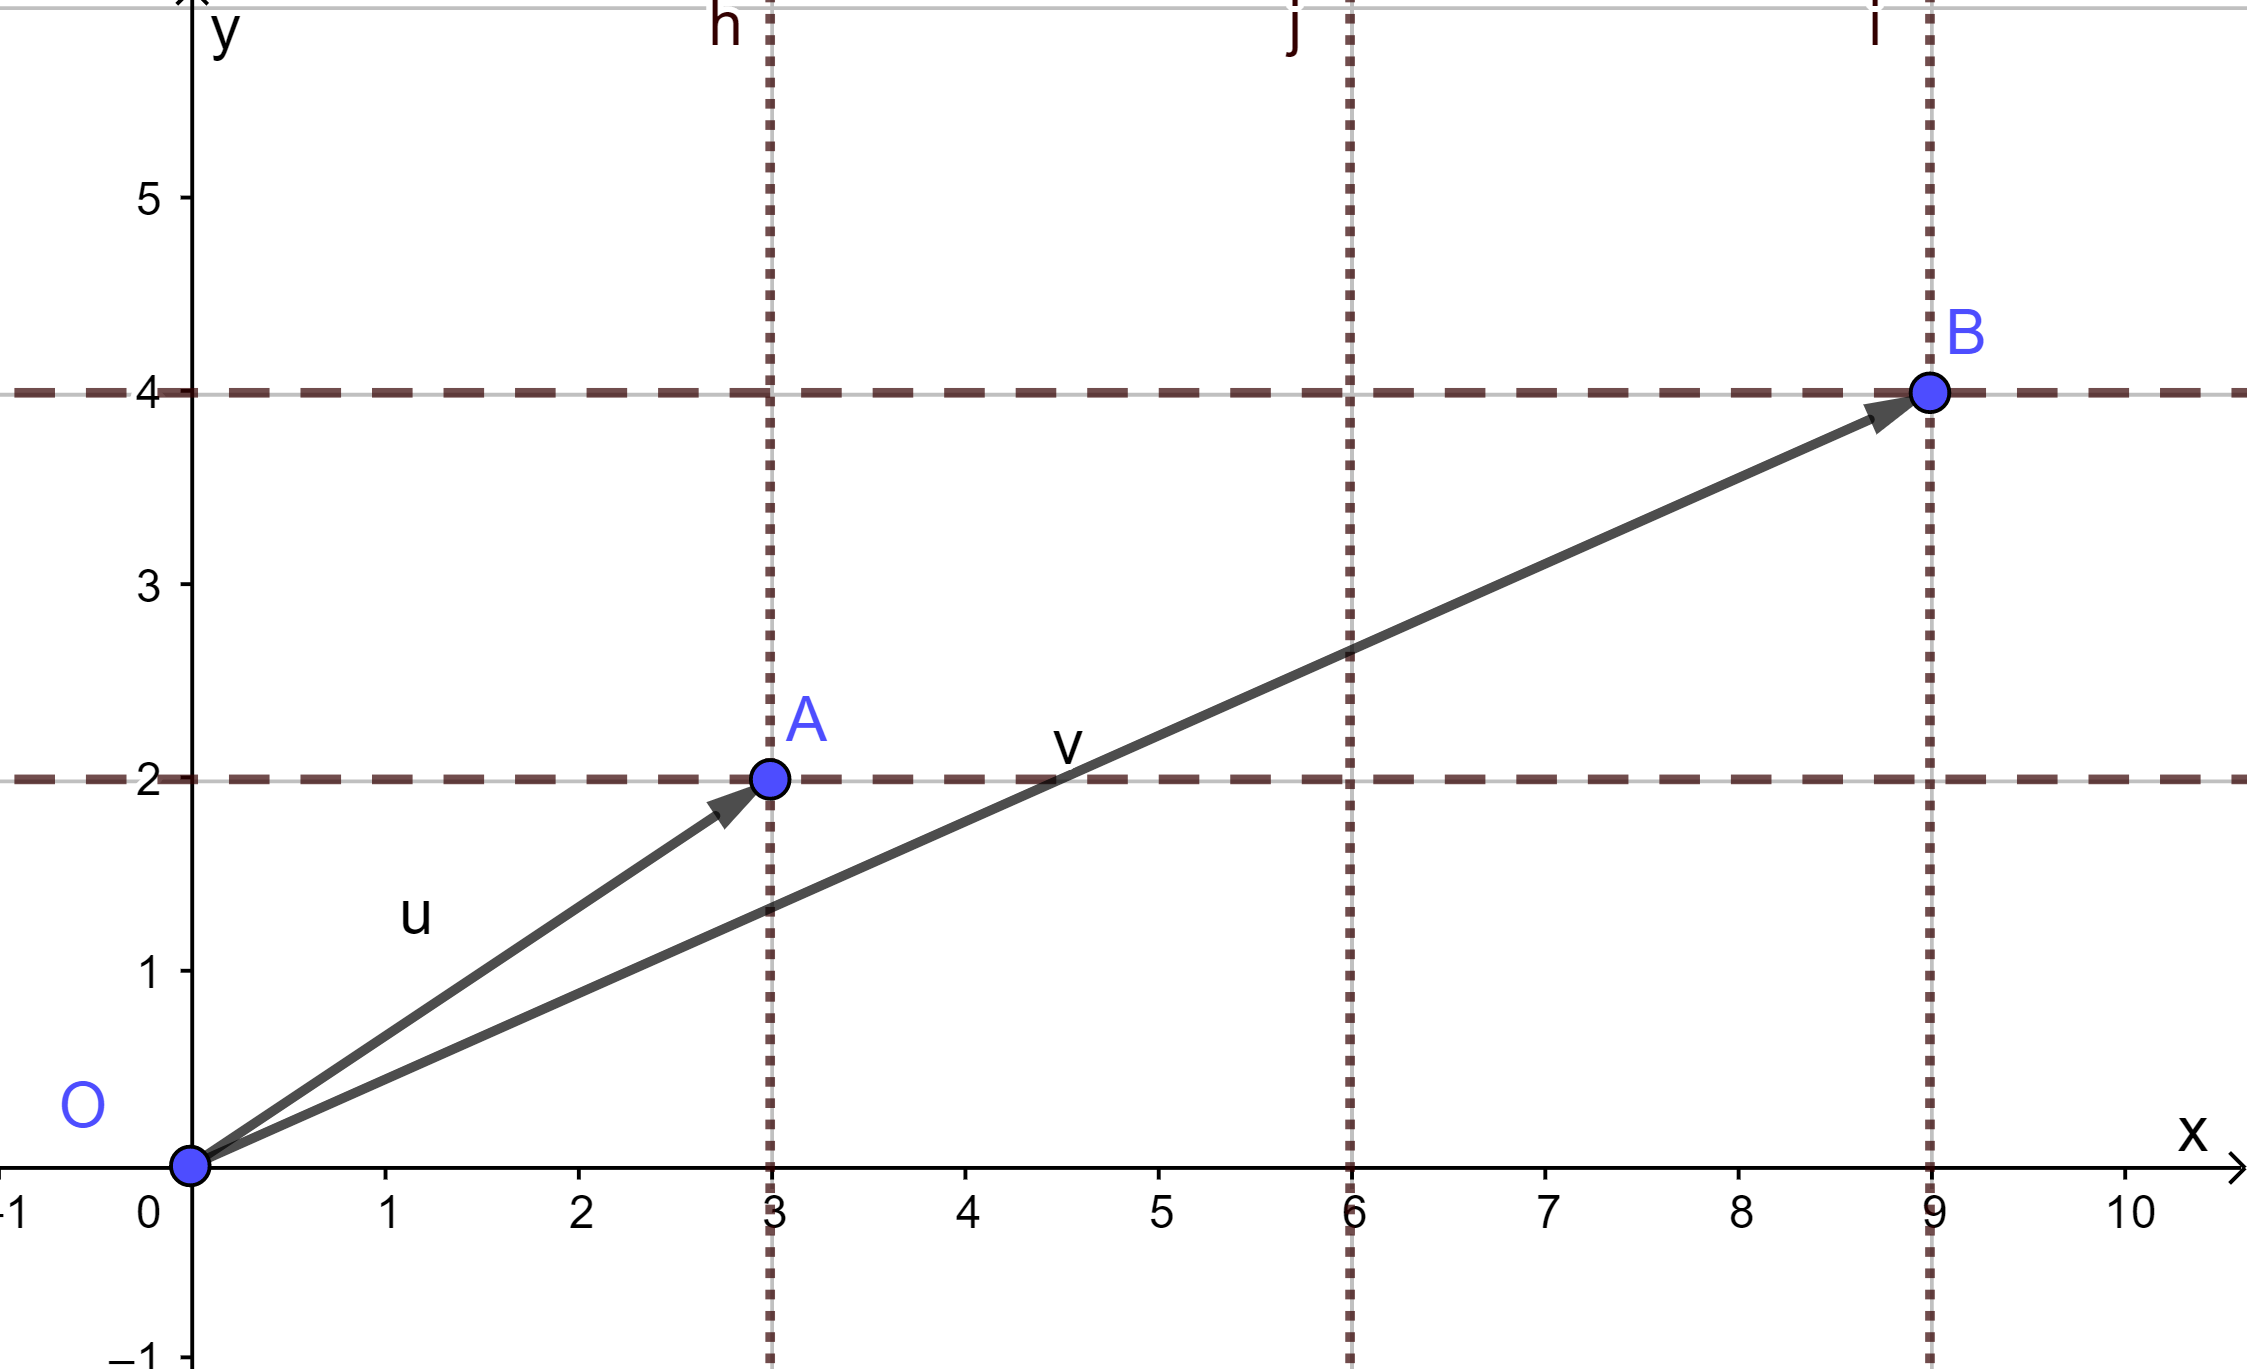
\includegraphics[width=\textwidth]{../Mathematik_1/Bilder/lineare_abbildungen_skalierung_ebene.png}
\end{minipage}
\begin{minipage}{0.5\textwidth}
\[
\begin{pmatrix}
x\\y
\end{pmatrix}
\mapsto
\begin{pmatrix}
3&0\\
0&2
\end{pmatrix}
\begin{pmatrix}
x\\y
\end{pmatrix}
=
\begin{pmatrix}
3x\\2y
\end{pmatrix}.
\]
\end{minipage}

\end{exabox}

\begin{exabox}{Drehung}{ }

\begin{minipage}{0.4\textwidth}
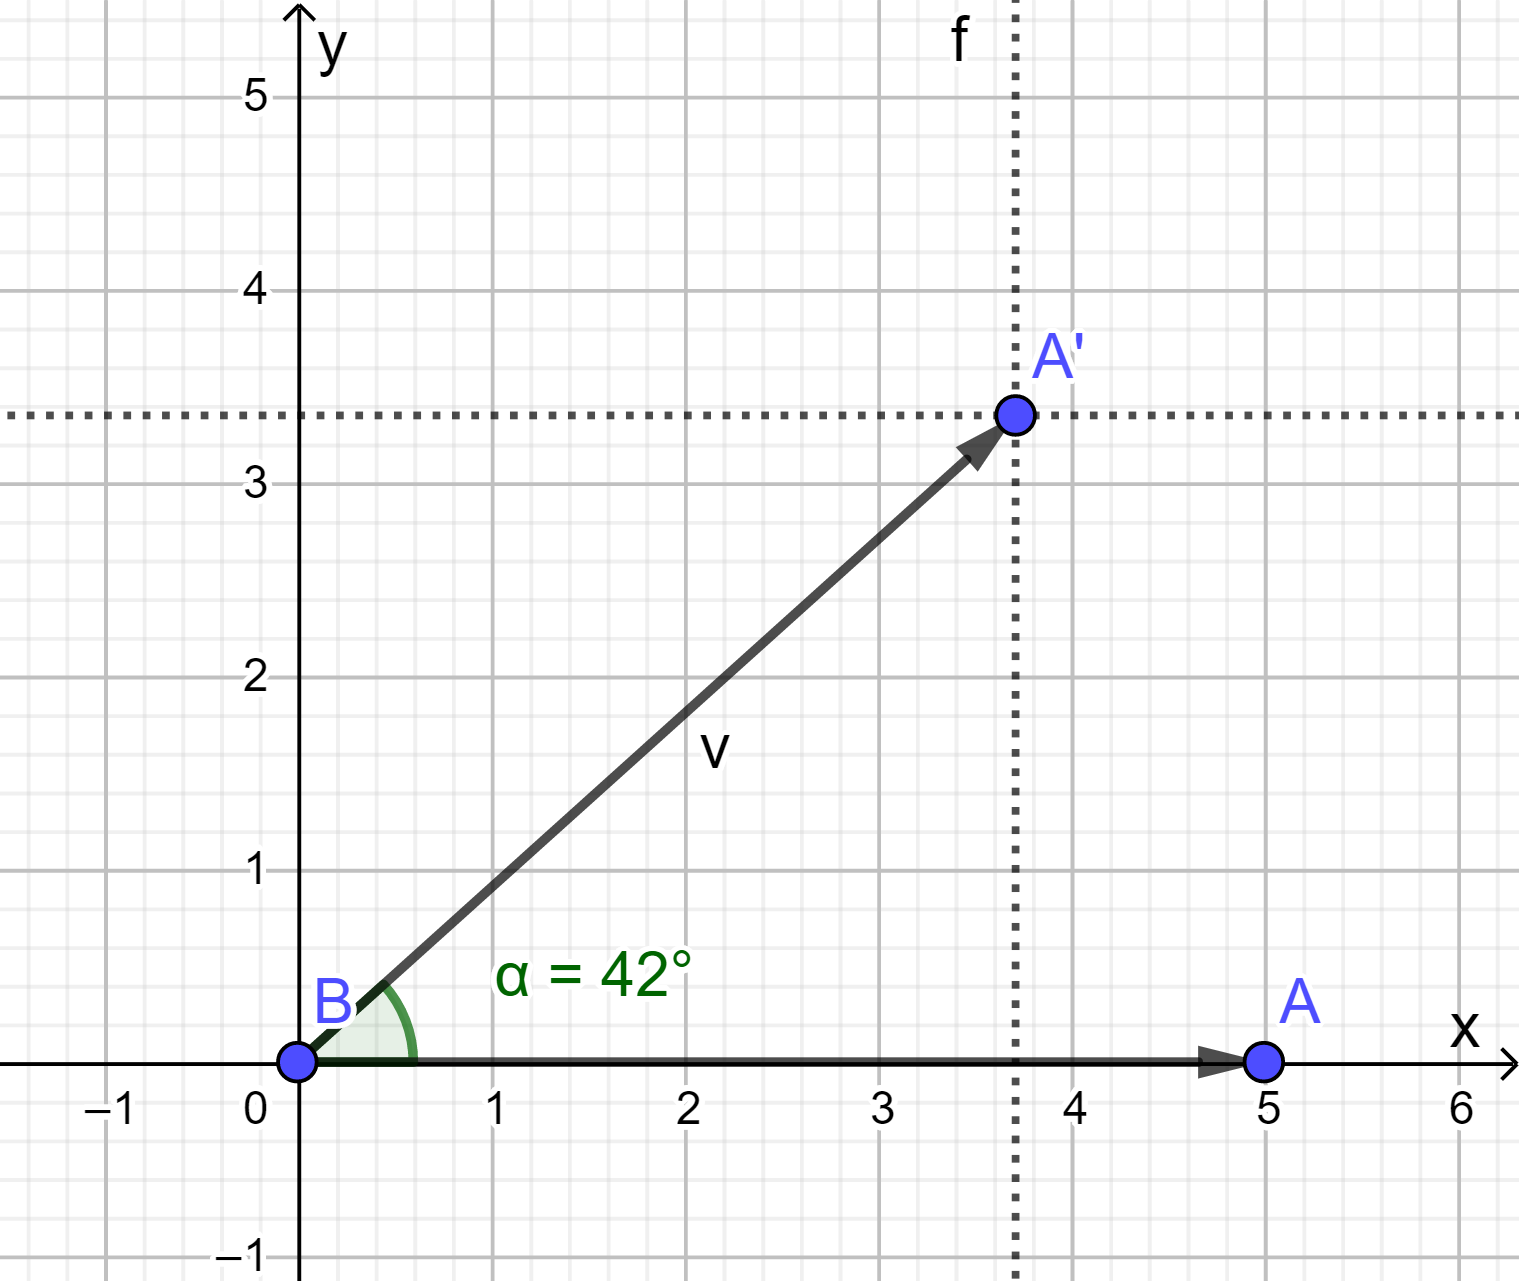
\includegraphics[width=\textwidth]{../Mathematik_1/Bilder/lineare_abbildungen_drehung_42_grad.png}
\end{minipage}
\begin{minipage}{0.55\textwidth}
\[
\begin{pmatrix}
x\\y
\end{pmatrix}
\mapsto
\underbrace{
\begin{pmatrix}
\cos\alpha&-\sin\alpha\\
\sin\alpha&\cos\alpha
\end{pmatrix}
}_{\textnormal{Drehmatrix}}
\begin{pmatrix}
x\\y
\end{pmatrix}.
\]
\end{minipage}

\end{exabox}

\noindent\textbf{Bemerkung:}
Eine Verschiebung um einen von Null verschiedenen Vektor ist keine lineare Abbildung. Jede lineare Abbildung erf�llt \(\mathcal A(\vec 0)=\vec 0\), w�hrend eine solche Verschiebung den Ursprung auf einen anderen Punkt abbildet.


\subsection{Matrix-Matrix-Multiplikation: Hintereinanderausf�hren}

Lineare Abbildungen k�nnen wie andere Funktionen miteinander verkettet werden. Sind
\[
\mathcal A:\mathbb K^n\to\mathbb K^p
\qquad\text{und}\qquad
\mathcal B:\mathbb K^p\to\mathbb K^m
\]
lineare Abbildungen, so ist auch ihre Komposition
\[
\mathcal B\circ\mathcal A:
\mathbb K^n\to\mathbb K^m
\]
linear.

Werden \(\mathcal A\) und \(\mathcal B\) durch die Matrizen \(A\) und \(B\) dargestellt, so gilt
\[
\mathcal B(\mathcal A(\vec x))
=
B(A\,\vec x)
=
(B\,A)\,\vec x.
\]

Die Matrixmultiplikation beschreibt damit das \textbf{Hintereinanderausf�hren linearer Abbildungen}.

\begin{defbox}{Matrix-Matrix-Multiplikation}{ }

F�r
\[
A\in\mathbb K^{m\times n},
\qquad
B\in\mathbb K^{n\times p}
\]
ist das Produkt
\[
	A\,B\in\mathbb K^{m\times p}
\]
durch
\[
	(A\,B)_{ij}
=
\sum_{k=1}^{n}a_{ik}b_{kj}
\]
definiert.

\end{defbox}

\begin{exabox}{Multiplikation}{ }

\[
\left(
\begin{array}{ccc}
\textcolor{brown}{1}&\textcolor{brown}{2}&\textcolor{brown}{3}\\
4&5&6
\end{array}
\right)
\left(
\begin{array}{cccc}
1&\textcolor{red}{0}&0&1\\
0&\textcolor{red}{3}&0&0\\
2&\textcolor{red}{4}&0&0
\end{array}
\right)
=
\left(
\begin{array}{cccc}
7&\textcolor{blue}{18}&0&1\\
16&39&0&4
\end{array}
\right),
\]
wobei beispielsweise
\[
(AB)_{\textcolor{blue}{12}}
=
\textcolor{brown}{1}\cdot\textcolor{red}{0}
+\textcolor{brown}{2}\cdot\textcolor{red}{3}
+\textcolor{brown}{3}\cdot\textcolor{red}{4}.
\]

\end{exabox}

\noindent\textbf{Bemerkung:}
Die Matrixmultiplikation ist assoziativ und distributiv, aber im Allgemeinen nicht kommutativ. Dies entspricht auch ihrer Interpretation als Hintereinanderausf�hren von Abbildungen: Die Reihenfolge der ausgef�hrten Transformationen kann das Ergebnis ver�ndern.

\begin{exabox}{Matrixmultiplikation ist im Allgemeinen nicht kommutativ}{ }

\[
{\color{brown}
\begin{pmatrix}
2&3\\4&5
\end{pmatrix}}
{\color{red}
\begin{pmatrix}
1&1\\0&1
\end{pmatrix}}
\neq
{\color{red}
\begin{pmatrix}
1&1\\0&1
\end{pmatrix}}
{\color{brown}
\begin{pmatrix}
2&3\\4&5
\end{pmatrix}}.
\]

\end{exabox}


\subsection{Bild und Rang: Welche Vektoren k�nnen herauskommen?}

Eine Matrix
\[
A\in\mathbb K^{m\times n}
\]
beschreibt eine lineare Abbildung von \(\mathbb K^n\) nach \(\mathbb K^m\). Dabei m�ssen jedoch nicht alle Vektoren der Zielmenge \(\mathbb K^m\) tats�chlich als Ergebnis der Abbildung auftreten.

Damit stellt sich die Frage, welche Vektoren durch die Abbildung �berhaupt erreicht werden k�nnen.

Die Menge aller Vektoren, die als \(A\vec x\) entstehen k�nnen, hei�t \textbf{Bild} (\emph{image}) der linearen Abbildung.

\begin{defbox}{Bild einer Matrix}{ }

F�r \(A\in\mathbb K^{m\times n}\) ist
\[
\operatorname{im}(A)
=
\left\{
\vec y\in\mathbb K^m:
\exists\,\vec x\in\mathbb K^n
\text{ mit }
\vec y=A\,\vec x
\right\}.
\]

\end{defbox}

Die zuvor betrachtete Spaltendarstellung liefert unmittelbar eine zweite Beschreibung des Bildes. Sind
\(\vec a_1,\ldots,\vec a_n\) die Spalten von \(A\), so gilt
\[
A\vec x
=
x_1\vec a_1+\cdots+x_n\vec a_n.
\]

Jeder Vektor im Bild ist daher eine Linearkombination der Spaltenvektoren.  Umgekehrt entsteht jede Linearkombination der Spalten durch eine geeignete Wahl der Komponenten von \(\vec x\). Damit gilt
\[
\operatorname{im}(A)
=
\operatorname{span}
\{\vec a_1,\ldots,\vec a_n\}.
\]

Das Bild einer Matrix ist somit ein Untervektorraum der Zielmenge \(\mathbb K^m\).

Die Dimension dieses Untervektorraums hei�t \textbf{Rang} (\emph{rank}) der Matrix.

\begin{defbox}{Rang einer Matrix}{ }

F�r \(A\in\mathbb K^{m\times n}\) ist
\[
\operatorname{rk}(A)
=
\dim\bigl(\operatorname{im}(A)\bigr).
\]

\end{defbox}

Der Rang beschreibt damit, wie viele voneinander unabh�ngige Richtungen im Bild der linearen Abbildung entstehen k�nnen. Wie der Rang einer konkreten Matrix systematisch bestimmt werden kann, wird im Zusammenhang mit linearen Gleichungssystemen untersucht.


\subsection{Kern und Defekt: Welche Vektoren verschwinden?}

Neben der Frage, welche Vektoren durch eine lineare Abbildung entstehen k�nnen, ist eine zweite Frage von grundlegender Bedeutung:

Welche Vektoren des Definitionsbereichs werden auf den Nullvektor \(\vec 0\) abgebildet?

Die Menge dieser Vektoren hei�t \textbf{Kern} (\emph{kernel}) der linearen Abbildung.

\begin{defbox}{Kern einer Matrix}{ }

F�r \(A\in\mathbb K^{m\times n}\) ist
\[
\ker(A)
=
\left\{
\vec x\in\mathbb K^n:
A\vec x=\vec 0
\right\}.
\]

\end{defbox}

Der Kern ist ein \underline{Untervektorraum}\randverweis{MA1-vektorraum} des Definitionsbereichs \(\mathbb K^n\). Enth�lt der Kern au�er dem Nullvektor weitere Vektoren, so werden verschiedene Vektoren durch die Abbildung auf denselben Vektor abgebildet. Denn aus
\[
	A\, \vec v=\vec0
\]
folgt f�r jeden Vektor \(\vec x\)
\[
	A\,(\vec x+\vec v) = A\,\vec x+A\,\vec v = A\vec x.
\]

Die Dimension des Kerns hei�t \textbf{Defekt} der Matrix.

\begin{defbox}{Defekt einer Matrix}{ }

F�r \(A\in\mathbb K^{m\times n}\) ist
\[
\operatorname{def}(A)
=
\dim\bigl(\ker(A)\bigr).
\]

\end{defbox}

Bild und Kern beschreiben damit zwei unterschiedliche Aspekte derselben linearen Abbildung: Das Bild beschreibt, welche Richtungen durch die Abbildung erreicht werden, w�hrend der Kern beschreibt, welche Richtungen bei der Abbildung auf den Nullvektor abgebildet werden.

Zwischen den Dimensionen dieser beiden Unterr�ume besteht ein grundlegender Zusammenhang.

\begin{theorembox}{Rangsatz}{ }

F�r \(A\in\mathbb K^{m\times n}\) gilt
\[
\operatorname{rk}(A)+\operatorname{def}(A)=n.
\]

\end{theorembox}

Der Rangsatz zerlegt die Dimension des Definitionsbereichs in zwei Anteile: die Dimension des Bildes und die Dimension des Kerns. Wie diese Gr��en f�r konkrete Matrizen bestimmt werden k�nnen, f�hrt unmittelbar zu den Methoden f�r lineare Gleichungssysteme.

 \newpage % Matrizen und lineare Abbildungen
\setcounter{exercise}{0} 
\ifintegriereaufgaben
\section*{Matrizen Aufgaben}\label{MA1-matrizen-aufgaben}

	Regeln und Beispiele, die zur Bearbeitung der Aufgaben hilfreich sind, finden Sie im Skript\wennreferenzvorhanden{MA1-matrizen}{ (Abschnitt \abschnittsverweis{MA1-matrizen})} und, falls Sie nicht weiterkommen, schauen Sie \hyperref[MA1-matrizen-loesungen]{hier}.
\else 
\section{Matrizen Aufgaben}\label{MA1-matrizen-aufgaben}

	Regeln und Beispiele, die zur Bearbeitung der Aufgaben hilfreich sind, finden Sie im Skript und, falls Sie nicht weiterkommen, schauen Sie \hyperref[MA1-matrizen-loesungen]{hier}.
\fi

\begin{exercisebox}[Rechenregeln]
	Berechnen Sie $ (  A^\intercal C - 2\cdot B)(-3\cdot C^\intercal )$ f�r die folgenden Matrizen
	\[ A = \left( \begin{array}{ccc} 1 & -2 & 3 \\ 0 & 3 & 1 \end{array}\right), \quad B = \left( \begin{array}{cc} 2 & -1 \\ 0 & 3 \\ -2 & -2 \end{array}\right), \quad C=\left( \begin{array}{cc} 3 & 2 \\ -1 & 2 \end{array}\right) \,. \]
\end{exercisebox}

%\begin{exercisebox}[Matrixmultiplikation und Skalarprodukt]
%Es sei $\boldsymbol a \in \mathbb R^n, \boldsymbol b\in \mathbb R^m$ und $A\in \mathbb R^{n\times m}$.  Zeigen Sie $\langle \boldsymbol a , A \boldsymbol b\rangle = \langle A^\intercal \boldsymbol a, \boldsymbol b \rangle\,.$
%\end{exercisebox}

\begin{exercisebox}[Rang und Bild]
	Es sei $A = \boldsymbol a \boldsymbol b^\intercal, \; \boldsymbol a \in \mathbb R^n, \boldsymbol b \in \mathbb R^m$. Wie ist der Rang der Matrix $A$? Wie sieht das Bild der Matrix aus?
\end{exercisebox}

\begin{exercisebox}[Basis]
	\begin{itemize}
		\item[(a)] F�r welche Werte von $a\in\mathbb R$ bilden die vier Vektoren eine Basis des $\mathbb R^4$?
  \begin{eqnarray*}
	  \boldsymbol x_1 = (3,1,4,0)^\intercal, \;  
	  \boldsymbol x_2 = (1,1,0,6)^\intercal, \; 
	  \boldsymbol x_3 = (-4,0,5,a)^\intercal, \;  
	  \boldsymbol x_4 = (0,0,1,2)^\intercal\,.
  \end{eqnarray*}

\item[(b)]	  �berpfr�fen Sie, ob die Polynome $1, 1+x, 1-x, x^2$ eine Basis des $\mathcal P_2$ bilden.
\end{itemize}
\end{exercisebox}

\begin{exercisebox}[Lineare Abbildungen]
	Gegeben sind die linearen Abbildungen 
	\[ \mathcal A: \mathbb R^2 \to \mathbb R^3, \left( \begin{array}{c} x_1 \\ x_2 \end{array}\right) \mapsto \left( \begin{array}{c} 0 \\ 3x_1-x_2 \\ 2x_2 \end{array}\right), \quad \mathcal B:\mathbb R^2 \to \mathbb R^3, \left( \begin{array}{c} x_1 \\ x_2 \end{array}\right) \mapsto \left( \begin{array}{c} -x_1+x_2 \\ -x_2 \\ 3x_2 \end{array}\right)\,.\]
	\begin{itemize}
		\item[(a)] Bestimmen Sie die darstellenden Matrizen $A$ und $B$ der linearen Abbildungen $\mathcal A$ und $\mathcal B$.
		\item[(b)] Gegeben ist eine Matrix \[ C=\left( \begin{array}{ccc} -1 & 2 & 0 \\ 0 & 3 & -1 \end{array}\right) \in \mathbb R^{2\times 3}\] Bestimmen Sie die von $C$ induzierte lineare Abbildung $\mathcal C$.
		\item[(c)] Wie lautet die darstellende Matrix der linearen Abbildung $\mathcal C\circ \mathcal A$?
	\end{itemize}
\end{exercisebox}

\begin{exercisebox}[Lineare Abbildungen]
	Gegeben sei der reelle Vektorraum \( \mathcal P_3:= \left\{ p:\mathbb R\to \mathbb R\;|\;p \;\textnormal{Polynome vom Grad } 3\right\}\) und die Abbildung \( f: \mathcal P_3 \to \mathbb R^2, \quad p\mapsto \left( \begin{array}{c}p(2) \\ p(3)\end{array}\right) \,.\)
	\begin{itemize}
		\item[(a)] Zeigen Sie, dass $f$ eine lineare Abbildung ist und berechnen Sie $f$ f�r die Monome $p_i: x\mapsto x^i,\; i=0,1,2,3\,.$
		\item[(b)] Berechnen Sie $f(p)$ f�r ein allgemeines Polynom $p \in \mathcal P_4$. % mit  \[ p=a_3\cdot p_3 + a_2 \cdot p_2 + a_1\cdot p_1 + a_0 \cdot p_0, \quad a_0,\dots,a_3\in \mathbb R.\] 
		\item[(d)] Zeigen Sie, dass die Funktion \[ g:\mathbb R^4 \to \mathbb R^2, \quad \left( \begin{array}{c}a_3 \\ a_2 \\ a_1 \\ a_0\end{array}\right) \mapsto f(a_3\cdot p_3 + a_2 \cdot p_2 + a_1\cdot p_1 + a_0 \cdot p_0)\] linear ist und berechnen Sie die darstellende Matrix von $g$.
	\end{itemize}
\end{exercisebox}

%\begin{exercisebox}[Mathematik lesen, Eigenwerte]
%\end{exercisebox}
%\begin{exercisebox}[Mathematik lesen, Eigenvektoren]
%\end{exercisebox}
%\begin{exercisebox}[Mathematik lesen, Positive Definitheit]
%\end{exercisebox}
%\begin{exercisebox}[Mathematik lesen, Symmetrie]
%\end{exercisebox}
%\begin{theorembox}[Grafikkarten Programmierung - cuda]
%\end{theorembox}
%\begin{theorembox}[D�nnbesetzte Matrizen]
%\end{theorembox}
%\begin{theorembox}[Hierarchische Matrizen, Niedrigrangapproximation]
%\end{theorembox}
%\begin{theorembox}[Spezielle Matrizen  (Elemente erg�nzen vielleicht?)- Mathematik lesen oder Beispiele angeben?]
%\begin{itemize}
%	\item Orthogonale Matrix
%	\item Komplex konjugierte
%	\item antisymmetrische Matrix
%	\item Singul�re Matrix
%	\item Transponierte
%	\item  $A \in \mathbb C^{2\times 3}$. Wie lautet $A^\intercal$? Konjugierte 
%	\item Basis des Vektorraums $\mathbb C^{2\times 3}$
%\end{itemize}
%\end{theorembox}
 \newpage 
\setcounter{satz}{0} \setcounter{def}{0} \setcounter{exa}{0}  \section{Lineare Gleichungssysteme}\label{MA1-lineare-gleichungssysteme}

\begin{table}[H]
  \centering
  \begin{tabularx}{\textwidth}{p{0.9\textwidth} p{0.1\textwidth}}
    \toprule
    \multicolumn{2}{c}{\textbf{�bersicht �ber Lernziele und Voraussetzungen}}\\
    \midrule
    \textbf{Lernziele} &\\[.5\normalbaselineskip]
    \tabitem lineare Gleichungssysteme in Gleichungs-, Vektor- und Matrixform darstellen &\\
    \tabitem lineare Gleichungssysteme mit dem Gau�schen Eliminationsverfahren systematisch l�sen &\\
    \tabitem die L�sbarkeit und Eindeutigkeit eines linearen Gleichungssystems mithilfe von Rang und Kern untersuchen &\\
    \tabitem die Struktur der L�sungsmenge eines linearen Gleichungssystems bestimmen und interpretieren &\\
    \tabitem Rang, Kern und Defekt einer Matrix mithilfe des Gau�schen Eliminationsverfahrens bestimmen &\\
    \tabitem die lineare Unabh�ngigkeit beziehungsweise Abh�ngigkeit gegebener Vektoren systematisch untersuchen &\\
    \midrule
    \textbf{Voraussetzungen} &\\[.5\normalbaselineskip]
    \tabitem Vektoren & \abschnittsverweis{MA1-vektoren}\\
    \tabitem Vektorr�ume, Linearkombinationen und lineare Unabh�ngigkeit & \abschnittsverweis{MA1-vektorraum}\\
    \tabitem Matrizen, lineare Abbildungen, Bild, Rang, Kern und Defekt & \abschnittsverweis{MA1-matrizen}\\
    \bottomrule
  \end{tabularx}
\end{table}

\ifintegriereaufgaben
\noindent �bungsaufgaben zum Thema finden sich hier:
\hyperref[MA1-lineare-gleichungssysteme-aufgaben]{Aufgaben}
\vspace{0.3cm}
\hrule
\fi


%----------------------------------------------------------
\subsection{Was ist ein lineares Gleichungssystem?}

Ein \textbf{lineares Gleichungssystem} (\emph{system of linear equations}) besteht aus mehreren linearen Gleichungen, die gleichzeitig erf�llt sein sollen. Die gesuchten Gr��en treten dabei nur in erster Potenz und jeweils mit konstanten Koeffizienten auf.

Ein Beispiel mit drei Gleichungen und vier Unbekannten ist
\[
(*)\qquad
\left\{
\begin{array}{rcrcrcrcl}
23x &+&45y&-&3z&+&4w&=&7,\\
    &&2y&-&z&+&6w&=&-3,\\
-15x&+&5y&&&-&3w&=&5.
\end{array}
\right.
\]

Eine L�sung des Gleichungssystems ist ein Vektor
\[
\begin{pmatrix}x&y&z&w\end{pmatrix}^{\intercal}\in\mathbb R^4,
\]
dessen Komponenten alle drei Gleichungen gleichzeitig erf�llen. Die L�sungsmenge \(\mathbb L\) ist daher eine Teilmenge von \(\mathbb R^4\).  Es ist zun�chst nicht klar, ob diese Menge �berhaupt Elemente enth�lt und, falls dies der Fall ist, ob sie aus einem einzigen oder aus mehreren Vektoren besteht.

Die Linearit�t der Gleichungen zeigt sich darin, dass ausschlie�lich konstante Vielfache der Unbekannten addiert werden. Terme wie \(\sin(x)\), \(y^2\) oder \(xz\) w�rden zu nichtlinearen Gleichungen f�hren.

Das Gleichungssystem kann zun�chst als Vektorgleichung gelesen werden.  Werden die Koeffizienten jeder Unbekannten zu einem Vektor zusammengefasst, so entsteht
\[
(*)\quad\Longleftrightarrow\quad
x
\begin{pmatrix}
23\\0\\-15
\end{pmatrix}
+
y
\begin{pmatrix}
45\\2\\5
\end{pmatrix}
+
z
\begin{pmatrix}
-3\\-1\\0
\end{pmatrix}
+
w
\begin{pmatrix}
4\\6\\-3
\end{pmatrix}
=
\begin{pmatrix}
7\\-3\\5
\end{pmatrix}.
\]

Damit erh�lt das L�sen des Gleichungssystems eine bereits bekannte Bedeutung: Gesucht sind Koeffizienten \(x,y,z,w\), mit denen sich der Vektor auf der rechten Seite als Linearkombination der vier Vektoren auf der linken Seite darstellen l�sst.

Werden diese vier Vektoren als Spalten einer Matrix angeordnet, entsteht schlie�lich die Matrixform des Gleichungssystems.

\begin{exabox}{Lineares Gleichungssystem in Matrixform}{ }

\[
(*)\quad\Longleftrightarrow\quad
\underbrace{
\begin{pmatrix}
23&45&-3&4\\
0&2&-1&6\\
-15&5&0&-3
\end{pmatrix}}_{\displaystyle A}
\underbrace{
\begin{pmatrix}
x\\y\\z\\w
\end{pmatrix}}_{\displaystyle\vec x}
=
\underbrace{
\begin{pmatrix}
7\\-3\\5
\end{pmatrix}}_{\displaystyle\vec b}.
\]

Kurz geschrieben lautet das Gleichungssystem damit
\[
A\vec x=\vec b.
\]

\end{exabox}

Die drei Schreibweisen beschreiben dasselbe mathematische Problem. Sie heben jedoch unterschiedliche Aspekte hervor: Die Gleichungsform zeigt die einzelnen Bedingungen, die Vektorform zeigt die gesuchte Linearkombination und die Matrixform erm�glicht eine systematische algebraische Bearbeitung.

Die zuvor eingef�hrten Begriffe\wennreferenzvorhanden{MA1-vektoren}{\wennreferenzvorhanden{MA1-matrizen}{ (Abschnitte \abschnittsverweis{MA1-vektoren}--\abschnittsverweis{MA1-matrizen})}} erm�glichen bereits eine strukturelle Beschreibung dieses Problems. F�r
\[
A\vec x=\vec b
\]
stellen sich insbesondere die Fragen, ob \(\vec b\) im Bild von \(A\) liegt und ob der Kern von \(A\) au�er dem Nullvektor weitere Vektoren enth�lt.  Damit h�ngen Existenz und Eindeutigkeit einer L�sung unmittelbar mit Bild, Rang, Kern und Defekt der Matrix zusammen.

Bisher wurden diese Begriffe vor allem inhaltlich beschrieben. Nun kommt eine systematische Rechenmethode hinzu. Das Gau�sche Eliminationsverfahren erm�glicht nicht nur das L�sen linearer Gleichungssysteme. Mit derselben Grundidee lassen sich auch Rang und Kern einer Matrix bestimmen und Fragen nach linearer Abh�ngigkeit, Erzeugendensystemen und Basen rechnerisch untersuchen.

Lineare Gleichungssysteme bilden damit den konkreten Ausgangspunkt f�r eine Rechenmethode, mit der sich mehrere der zuvor eingef�hrten Begriffe der linearen Algebra praktisch untersuchen lassen.


%----------------------------------------------------------
\subsection{Existenz und Eindeutigkeit von L�sungen}

Bevor konkrete Gleichungssysteme gel�st werden, lassen sich die Fragen nach Existenz und Eindeutigkeit bereits mithilfe von Bild und Kern einer Matrix beschreiben.

Es sei
\[
A\in\mathbb R^{m\times n},
\qquad
\vec x\in\mathbb R^n,
\qquad
\vec b\in\mathbb R^m.
\]
Das lineare Gleichungssystem
\[
A\vec x=\vec b
\]
ist genau dann l�sbar, wenn es einen Vektor \(\vec x\) gibt, der durch \(A\) auf \(\vec b\) abgebildet wird.

Nach der Definition des Bildes bedeutet dies gerade, dass \(\vec b\) im Bild von \(A\) liegen muss.

\begin{theorembox}{Bedingung f�r die L�sbarkeit eines linearen Gleichungssystems}{ }

Das lineare Gleichungssystem
\[
A\vec x=\vec b
\]
besitzt mindestens eine L�sung genau dann, wenn
\[
\vec b\in\operatorname{im}(A).
\]

\end{theorembox}

Damit beantwortet der Begriff des Bildes die Frage nach der \textbf{Existenz} einer L�sung.

Nach der Existenz stellt sich die Frage nach der Eindeutigkeit. Angenommen, \(\vec x_1\) und \(\vec x_2\) seien zwei L�sungen desselben Gleichungssystems. Dann gilt
\[
A\vec x_1=A\vec x_2=\vec b.
\]
Durch Subtraktion folgt
\[
A(\vec x_1-\vec x_2)=\vec0.
\]

Die Differenz zweier L�sungen liegt also im Kern von \(A\).

Ein Gleichungssystem mit rechter Seite \(\vec0\),
\[
A\vec x=\vec0,
\]
hei�t \textbf{homogenes lineares Gleichungssystem} (\emph{homogeneous system of linear equations}). Ein Gleichungssystem mit einer von Null verschiedenen rechten Seite wird entsprechend \textbf{inhomogen} genannt.

Besitzt das homogene Gleichungssystem nur die triviale L�sung \(\vec x=\vec0\), so kann die Differenz zweier L�sungen nur der Nullvektor sein. In diesem Fall m�ssen zwei m�gliche L�sungen identisch sein.

Besitzt das homogene Gleichungssystem dagegen eine nichttriviale L�sung \(\vec v\neq\vec0\), so gilt
\[
A\vec v=\vec0.
\]
Ist \(\vec x_s\) eine L�sung von \(A\vec x=\vec b\), dann ist auch
\[
A(\vec x_s+\vec v)
=
A\vec x_s+A\vec v
=
\vec b.
\]
Eine vorhandene L�sung kann dann also nicht eindeutig sein.

\begin{theorembox}{Bedingung f�r die Eindeutigkeit einer L�sung}{ }

Das lineare Gleichungssystem
\[
A\vec x=\vec b
\]
besitzt h�chstens eine L�sung genau dann, wenn
\[
\ker(A)=\{\vec0\}.
\]

Besitzt das Gleichungssystem zus�tzlich mindestens eine L�sung, so ist diese L�sung eindeutig.

\end{theorembox}

Damit beantworten zwei der Begriffe aus dem vorangegangenen Abschnitt die beiden grundlegenden Fragen:
\[
\vec b\in\operatorname{im}(A)
\quad\Longleftrightarrow\quad
\text{Existenz einer L�sung},
\]
w�hrend
\[
\ker(A)=\{\vec0\}
\quad\Longleftrightarrow\quad
\text{h�chstens eine L�sung}
\]
gilt.

F�r eine eindeutig bestimmte L�sung m�ssen beide Bedingungen gleichzeitig erf�llt sein.


%----------------------------------------------------------
\subsection{Das Gau�sche Eliminationsverfahren}

Die bisherigen �berlegungen beschreiben, welche Bedingungen �ber L�sbarkeit und Eindeutigkeit entscheiden. F�r eine konkrete Matrix fehlt jedoch noch ein systematisches Verfahren, mit dem diese Bedingungen �berpr�ft und die L�sungen tats�chlich bestimmt werden k�nnen.

Dazu sei ein allgemeines lineares Gleichungssystem
\[
\begin{pmatrix}
a_{11}&\cdots&a_{1n}\\
\vdots&\ddots&\vdots\\
a_{m1}&\cdots&a_{mn}
\end{pmatrix}
\begin{pmatrix}
x_1\\
\vdots\\
x_n
\end{pmatrix}
=
\begin{pmatrix}
b_1\\
\vdots\\
b_m
\end{pmatrix}
\]
mit
\[
A\in\mathbb R^{m\times n},
\qquad
\vec x\in\mathbb R^n,
\qquad
\vec b\in\mathbb R^m
\]
gegeben.

Je nach Anzahl der Gleichungen und Unbekannten hei�t das Gleichungssystem

\begin{itemize}
  \item \textbf{unterbestimmt}, wenn es mehr Unbekannte als Gleichungen gibt,
  also \(n>m\),
  \item \textbf{quadratisch}, wenn es ebenso viele Unbekannte wie Gleichungen
  gibt, also \(n=m\),
  \item \textbf{�berbestimmt}, wenn es mehr Gleichungen als Unbekannte gibt,
  also \(m>n\).
\end{itemize}

Allein aus dieser Einteilung l�sst sich im Allgemeinen noch nicht entscheiden, ob ein konkretes Gleichungssystem l�sbar ist. Daf�r m�ssen die Gleichungen selbst untersucht werden.

Das grundlegende Verfahren daf�r ist das \textbf{Gau�sche Eliminationsverfahren} (\emph{Gaussian elimination}).  Seine Idee besteht darin, ein Gleichungssystem durch �quivalenzumformungen schrittweise in eine Form zu �berf�hren, aus der sich die L�sungen und weitere Eigenschaften des Systems leichter ablesen lassen.


%----------------------------------------------------------
\subsubsection*{Elementare Zeilenumformungen}

Bereits bei einzelnen Gleichungen wurden �quivalenzumformungen verwendet: Eine Gleichung wird ver�ndert, ohne ihre L�sungsmenge zu ver�ndern. Beim Gau�schen Eliminationsverfahren wird dieselbe Idee auf ein ganzes Gleichungssystem �bertragen.

Dabei sind drei grundlegende Umformungen zul�ssig:

\begin{enumerate}
  \item Zwei Gleichungen k�nnen miteinander vertauscht werden.
  \item Eine Gleichung kann mit einem von Null verschiedenen Skalar multipliziert werden.
  \item Zu einer Gleichung kann ein Vielfaches einer anderen Gleichung
  addiert werden.
\end{enumerate}

Diese Operationen ver�ndern die L�sungsmenge des Gleichungssystems nicht.  In Matrixdarstellung entsprechen sie den \textbf{elementaren Zeilenumformungen} (\emph{elementary row operations}).

Da beim L�sen eines inhomogenen Gleichungssystems auch die rechte Seite von jeder Umformung betroffen ist, werden Koeffizientenmatrix und rechte Seite gemeinsam in der \textbf{erweiterten Matrix} (\emph{augmented matrix}) zusammengefasst:

\[
A\vec x=\vec b
\qquad\longrightarrow\qquad
A_{\vec b}:=
\left(
\begin{array}{ccc|c}
a_{11}&\cdots&a_{1n}&b_1\\
\vdots&\ddots&\vdots&\vdots\\
a_{m1}&\cdots&a_{mn}&b_m
\end{array}
\right).
\]

Jede Zeile dieser erweiterten Matrix steht weiterhin f�r eine Gleichung des urspr�nglichen Gleichungssystems.


%----------------------------------------------------------
\subsubsection*{Zeilenstufenform}

Ziel des Gau�schen Eliminationsverfahrens ist es zun�chst, durch elementare Zeilenumformungen unterhalb geeigneter f�hrender Eintr�ge Nullen zu erzeugen.  Dadurch entsteht schrittweise eine \textbf{Zeilenstufenform} (\emph{row echelon form}), die auch als Trapezform bezeichnet wird.

In einer Zeilenstufenform liegen die f�hrenden von Null verschiedenen Eintr�ge aufeinanderfolgender Zeilen jeweils weiter rechts. Vollst�ndig aus Nullen bestehende Zeilen stehen am unteren Ende der Matrix.  

Das L�sen erfolgt damit in zwei Schritten:

\begin{enumerate}
  \item Die erweiterte Matrix \(A_{\vec b}\) wird durch elementare Zeilenumformungen in Zeilenstufenform gebracht.
  \item Anschlie�end werden die zugeh�rigen Gleichungen von unten nach oben aufgel�st.
\end{enumerate}

Die Zeilenstufenform liefert jedoch mehr als nur einen bequemeren Weg zur L�sung. An ihr werden auch Rang, freie Unbekannte und m�gliche Widerspr�che sichtbar. Dadurch verbindet das Gau�sche Eliminationsverfahren das eigentliche L�sen mit den zuvor eingef�hrten strukturellen Begriffen.


%----------------------------------------------------------
\subsubsection*{L�sbarkeit und Eindeutigkeit aus dem Rang}

Die erweiterte Matrix erlaubt es, die Frage
\[
\vec b\in\operatorname{im}(A)
\]
rechnerisch zu untersuchen.

Die Spalten von \(A\) spannen das Bild von \(A\) auf. Wird die rechte Seite \(\vec b\) als zus�tzliche Spalte erg�nzt, gibt es zwei M�glichkeiten: Entweder liegt \(\vec b\) bereits im von den Spalten von \(A\) aufgespannten Raum, oder durch die zus�tzliche Spalte entsteht eine weitere unabh�ngige Richtung.

Im ersten Fall ver�ndert sich der Rang nicht. Im zweiten Fall erh�ht sich der Rang durch das Hinzuf�gen von \(\vec b\). Genau dann kann \(\vec b\) nicht als Linearkombination der Spalten von \(A\) dargestellt werden und das Gleichungssystem besitzt keine L�sung.

\begin{theorembox}{L�sbarkeit und Eindeutigkeit aus dem Rang}{ }

Es sei
\[
A\in\mathbb R^{m\times n}.
\]
Dann gilt:

\begin{itemize}
  \item
  \(\operatorname{rk}(A)\neq\operatorname{rk}(A_{\vec b})\)

  \(\Rightarrow\) Das Gleichungssystem ist nicht l�sbar.

  \item
  \(\operatorname{rk}(A)=\operatorname{rk}(A_{\vec b})<n\)

  \(\Rightarrow\) Das Gleichungssystem besitzt unendlich viele L�sungen.

  \item
  \(\operatorname{rk}(A)=\operatorname{rk}(A_{\vec b})=n\)

  \(\Rightarrow\) Das Gleichungssystem besitzt genau eine L�sung.
\end{itemize}

\end{theorembox}

Damit werden die abstrakten Bedingungen �ber Bild und Kern durch ein konkretes Rechenverfahren zug�nglich.


%----------------------------------------------------------
\subsection{Beispiele zum Gau�schen Eliminationsverfahren}

Die verschiedenen M�glichkeiten f�r die L�sungsmenge werden nun an konkreten Gleichungssystemen sichtbar.


%----------------------------------------------------------
\begin{exabox}{Beispiel \(1\): \(\operatorname{rk}(A)\neq\operatorname{rk}(A_{\vec b})\)}{ }

Es ist \(A\in\mathbb R^{2\times2}\) beziehungsweise \(A_{\vec b}\in\mathbb R^{2\times3}\) mit
\[
A_{\vec b}
=
\left(
\begin{array}{cc|c}
1&3&5\\
2&6&7
\end{array}
\right).
\]

Durch �quivalente Zeilenumformungen entsteht die Zeilenstufenform
\[
\left(
\begin{array}{cc|c}
1&3&5\\
0&0&-3
\end{array}
\right).
\]

Die zweite Zeile entspricht der Gleichung
\[
0=-3.
\]
Damit ist unmittelbar ein Widerspruch entstanden. Das Gleichungssystem ist also nicht l�sbar.

Dies l�sst sich zugleich �ber die R�nge ausdr�cken:
\[
\operatorname{rk}(A)=1
\neq
\operatorname{rk}(A_{\vec b})=2.
\]

Die zus�tzliche Spalte \(\vec b\) erh�ht den Rang. Der Vektor \(\vec b\) liegt daher nicht im Bild von \(A\), und die L�sungsmenge ist
\[
\mathbb L=\emptyset.
\]

\end{exabox}


%----------------------------------------------------------
\begin{exabox}{Beispiel \(2\): \(\operatorname{rk}(A)=\operatorname{rk}(A_{\vec b})<n\)}{ }

Es ist \(A\in\mathbb R^{3\times4}\) beziehungsweise \(A_{\vec b}\in\mathbb R^{3\times5}\) mit
\[
A_{\vec b}
=
\left(
\begin{array}{rrrr|r}
1&0&0&1&0\\
0&1&0&1&1\\
2&0&1&0&-4
\end{array}
\right).
\]

Durch �quivalente Zeilenumformungen entsteht die Zeilenstufenform
\[
\left(
\begin{array}{rrrr|r}
1&0&0&1&0\\
0&1&0&1&1\\
0&0&1&-2&-4
\end{array}
\right).
\]

Damit gilt
\[
\operatorname{rk}(A)
=
\operatorname{rk}(A_{\vec b})
=
3<n=4.
\]

Das Gleichungssystem ist also l�sbar, aber die L�sung ist nicht eindeutig.  Da vier Unbekannte vorhanden sind, aber nur drei f�hrende Unbekannte auftreten, bleibt eine Unbekannte frei.

F�r \(x_4\) kann daher ein Parameter
\[
x_4=\alpha\in\mathbb R
\]
gew�hlt werden. Die �brigen Gleichungen werden von unten nach oben aufgel�st:
\[
\begin{cases}
x_4 &= \alpha,\\
x_3 &= -4+2x_4
      \Rightarrow x_3=-4+2\alpha,\\
x_2 &= 1-x_4
      \Rightarrow x_2=1-\alpha,\\
x_1 &= -x_4
      \Rightarrow x_1=-\alpha.
\end{cases}
\]

Damit ergibt sich
\[
\vec x
=
\begin{pmatrix}
-\alpha\\
-4+2\alpha\\
1-\alpha\\
\alpha
\end{pmatrix}
=
\underbrace{
\begin{pmatrix}
0\\
-4\\
1\\
0
\end{pmatrix}}_{\displaystyle\vec x_s}
+
\alpha
\underbrace{
\begin{pmatrix}
-1\\
2\\
-1\\
1
\end{pmatrix}}_{\displaystyle\vec x_h}.
\]

Dabei gilt
\[
A\vec x_s=\vec b
\]
und
\[
A\vec x_h=\vec0.
\]

Der Vektor \(\vec x_s\) ist also eine spezielle L�sung des inhomogenen Gleichungssystems. Der Vektor \(\vec x_h\) ist eine nichttriviale L�sung des zugeh�rigen homogenen Gleichungssystems und liegt damit im Kern von \(A\).  

Da in diesem Beispiel nur ein freier Parameter auftritt, gilt sogar
\[
\ker(A)
=
\operatorname{span}\{\vec x_h\}.
\]

\medskip
\noindent\textbf{Erkenntnis:}

Die gesamte L�sungsmenge entsteht aus einer speziellen L�sung und allen Vektoren des Kerns:
\[
\mathbb L
=
\vec x_s+\ker(A)
=
\left\{
\vec x_s+\vec x_h:
\vec x_h\in\ker(A)
\right\}.
\]

In diesem Beispiel besitzt der Kern die Dimension \(1\). Daher gilt
\[
\operatorname{def}(A)=1.
\]

\end{exabox}


%----------------------------------------------------------
\begin{exabox}{Beispiel \(3\): quadratisches Gleichungssystem mit nicht eindeutiger L�sung}{ }

Es ist \(A\in\mathbb R^{4\times4}\) beziehungsweise
\(A_{\vec b}\in\mathbb R^{4\times5}\) mit
\[
A_{\vec b}
=
\left(
\begin{array}{rrrr|r}
1&2&-1&1&1\\
1&4&3&1&3\\
-1&-1&3&2&6\\
3&6&-3&4&5
\end{array}
\right)
\Longleftrightarrow
\left(
\begin{array}{rrrr|r}
1&2&-1&1&1\\
0&1&2&0&1\\
0&0&0&1&2\\
0&0&0&0&0
\end{array}
\right).
\]

Aus der Zeilenstufenform folgt
\[
\operatorname{rk}(A)
=
\operatorname{rk}(A_{\vec b})
=
3<n=4.
\]

Das Gleichungssystem ist damit l�sbar, aber nicht eindeutig. Obwohl das urspr�ngliche Gleichungssystem ebenso viele Gleichungen wie Unbekannte besitzt, sind nicht alle vier Gleichungen voneinander unabh�ngig. Der Rang betr�gt nur \(3\).

Die Variable \(x_3\) kann frei gew�hlt werden:
\[
x_3=\alpha\in\mathbb R.
\]
Von unten nach oben folgt
\[
\begin{cases}
x_4 &= 2,\\
x_3 &= \alpha,\\
x_2 &= 1-2x_3
      \Rightarrow x_2=1-2\alpha,\\
x_1 &= 1-2x_2+x_3-x_4
      \Rightarrow x_1=-3+5\alpha.
\end{cases}
\]

Damit ergibt sich
\[
\vec x
=
\begin{pmatrix}
-3+5\alpha\\
1-2\alpha\\
\alpha\\
2
\end{pmatrix}
=
\underbrace{
\begin{pmatrix}
-3\\
1\\
0\\
2
\end{pmatrix}}_{\displaystyle\vec x_s}
+
\alpha
\underbrace{
\begin{pmatrix}
5\\
-2\\
1\\
0
\end{pmatrix}}_{\displaystyle\vec x_h}.
\]

Wieder gilt
\[
A\vec x_s=\vec b,
\qquad
A\vec x_h=\vec0.
\]

Damit ist
\[
\ker(A)
=
\operatorname{span}
\left\{
\begin{pmatrix}
5\\-2\\1\\0
\end{pmatrix}
\right\}
\]
und
\[
\operatorname{def}(A)=1.
\]

\medskip
\noindent\textbf{Erkenntnis:}

Auch ein quadratisches Gleichungssystem muss nicht eindeutig l�sbar sein.  Entscheidend ist nicht allein die Anzahl der Gleichungen und Unbekannten, sondern der Rang der Koeffizientenmatrix.

Ist der Kern nicht trivial, so besitzt ein l�sbares Gleichungssystem mehrere L�sungen. Allgemein gilt wiederum
\[
\mathbb L=\vec x_s+\ker(A).
\]

\end{exabox}


%----------------------------------------------------------
\begin{exabox}{Beispiel \(4\): eindeutig l�sbares quadratisches Gleichungssystem}{ }

Es ist \(A\in\mathbb R^{4\times4}\) beziehungsweise \(A_{\vec b}\in\mathbb R^{4\times5}\) mit
\[
A_{\vec b}
=
\left(
\begin{array}{rrrr|r}
2&4&0&4&8\\
1&3&1&4&10\\
-2&-2&1&1&7\\
0&-1&0&1&-1
\end{array}
\right)
\Longleftrightarrow
\left(
\begin{array}{rrrr|r}
2&4&0&4&8\\
0&-2&-2&-4&-12\\
0&0&-1&1&3\\
0&0&0&8&16
\end{array}
\right).
\]

In jeder der vier Spalten der Koeffizientenmatrix befindet sich eine Pivotposition. Daher gilt
\[
\operatorname{rk}(A)
=
\operatorname{rk}(A_{\vec b})
=
4=n.
\]

Damit ist das Gleichungssystem eindeutig l�sbar. Gleichzeitig folgt aus dem Rangsatz
\[
\operatorname{def}(A)
=
n-\operatorname{rk}(A)
=
4-4
=
0,
\]
also
\[
\ker(A)=\{\vec0\}.
\]

Die L�sung wird von unten nach oben bestimmt:
\[
\begin{cases}
8x_4 &=16
       \Rightarrow x_4=2,\\
-x_3 &=3-x_4=3-2
       \Rightarrow x_3=-1,\\
-2x_2 &=-12+2x_3+4x_4
       =-12-2+8
       \Rightarrow x_2=3,\\
2x_1 &=8-4x_2-4x_4
       =8-12-8
       \Rightarrow x_1=-6.
\end{cases}
\]

Damit lautet die eindeutig bestimmte L�sung
\[
\vec x
=
\begin{pmatrix}
-6\\
3\\
-1\\
2
\end{pmatrix}.
\]

\medskip
\noindent\textbf{Erkenntnis:}

In diesem Beispiel ist \(A\) quadratisch und besitzt vollen Rang:
\[
\operatorname{rk}(A)=4.
\]
Damit gilt sowohl
\[
\ker(A)=\{\vec0\}
\]
als auch
\[
\operatorname{im}(A)=\mathbb R^4.
\]

Das bedeutet: F�r jede rechte Seite \(\vec b\in\mathbb R^4\) besitzt das Gleichungssystem \(A\vec x=\vec b\) genau eine L�sung.

Diese besondere Eigenschaft quadratischer Matrizen f�hrt im folgenden Abschnitt zum Begriff der inversen Matrix.

\end{exabox}


%----------------------------------------------------------
\begin{exabox}{Beispiel \(5\): �berbestimmtes, nicht l�sbares Gleichungssystem}{ }

Es ist \(A\in\mathbb R^{4\times3}\) beziehungsweise \(A_{\vec b}\in\mathbb R^{4\times4}\) mit
\[
A_{\vec b}
=
\left(
\begin{array}{rrr|r}
1&-1&1&0\\
3&2&1&2\\
1&2&4&0\\
-1&7&1&2
\end{array}
\right)
\Longleftrightarrow
\left(
\begin{array}{rrr|r}
1&-1&1&0\\
0&5&-2&2\\
0&0&-7&2\\
0&0&-11&1
\end{array}
\right).
\]

Die letzten beiden Zeilen enthalten Bedingungen an dieselbe verbleibende Unbekannte, die nicht gleichzeitig erf�llt werden k�nnen. Durch eine weitere Zeilenumformung entsteht entsprechend eine Widerspruchszeile.

Dies zeigt sich auch an den R�ngen:
\[
\operatorname{rk}(A)=3
\neq
\operatorname{rk}(A_{\vec b})=4.
\]

Die rechte Seite \(\vec b\) liegt also nicht im Bild von \(A\). F�r die gegebene rechte Seite ist das Gleichungssystem nicht l�sbar und
\[
\mathbb L=\emptyset.
\]

\medskip
\noindent\textbf{Erkenntnis:}

Bei einem �berbestimmten Gleichungssystem mit \(m>n\) gibt es mehr Gleichungen als Unbekannte. Ob eine L�sung existiert, h�ngt davon ab, ob die rechte Seite mit allen Bedingungen vertr�glich ist.

�berbestimmt bedeutet daher nicht automatisch unl�sbar. Entscheidend bleibt die Bedingung
\[
\operatorname{rk}(A)=\operatorname{rk}(A_{\vec b}).
\]

\end{exabox}


\subsection{Das Gau�verfahren als Werkzeug der linearen Algebra}

Das Gau�sche Eliminationsverfahren wurde ausgehend von linearen
Gleichungssystemen entwickelt. Mit derselben Systematik lassen sich jedoch
auch mehrere der zuvor eingef�hrten Begriffe der linearen Algebra
rechnerisch untersuchen.

Ausgangspunkt sei eine Matrix
\[
A\in\mathbb R^{m\times n}
\]
mit Rang \(k\). Durch elementare Zeilenumformungen kann \(A\) in
Zeilenstufenform gebracht werden. Die umgeformte Matrix wird im Folgenden
mit \(\widetilde A\) bezeichnet. Schematisch hat sie die Form
\[
A
\quad\longrightarrow\quad
\widetilde A
=
\left(
\begin{array}{cccccc}
a_{11} & a_{12} & \cdots & a_{1k} & \cdots & a_{1n}\\
0 & \widetilde a_{22} & \cdots & \widetilde a_{2k}
  & \cdots & \widetilde a_{2n}\\
\vdots & \ddots & \ddots & \vdots & \ddots & \vdots\\
0 & \cdots & 0 & \widetilde a_{kk}
  & \cdots & \widetilde a_{kn}\\
\vdots & \ddots & \ddots & 0 & \ddots & 0\\
0 & \cdots & 0 & 0 & \cdots & 0
\end{array}
\right).
\]

Die Tilde kennzeichnet dabei Eintr�ge, die durch die Zeilenumformungen
ver�ndert wurden. Da \(\operatorname{rk}(A)=k\) gilt, besitzt
\(\widetilde A\) genau \(k\) von Null verschiedene Zeilen beziehungsweise
\(k\) Pivotpositionen.

Diese Struktur erm�glicht es, Rang, Bild, Kern und Defekt sowie Fragen nach
linearer Unabh�ngigkeit mit demselben Verfahren systematisch zu
untersuchen.


%----------------------------------------------------------
\subsubsection*{Den Rang einer Matrix bestimmen}

Der Rang einer Matrix wurde als Dimension ihres Bildes definiert:
\[
\operatorname{rk}(A)
=
\dim\bigl(\operatorname{im}(A)\bigr).
\]

Das Gau�sche Eliminationsverfahren liefert nun eine systematische
M�glichkeit, diesen Rang zu bestimmen. Wird eine Matrix durch elementare
Zeilenumformungen in Zeilenstufenform �berf�hrt, so werden die voneinander
unabh�ngigen Bedingungen sichtbar.

Besitzt die Zeilenstufenform \(k\) von Null verschiedene Zeilen, so befinden
sich darunter nur noch Nullzeilen.

\begin{center}
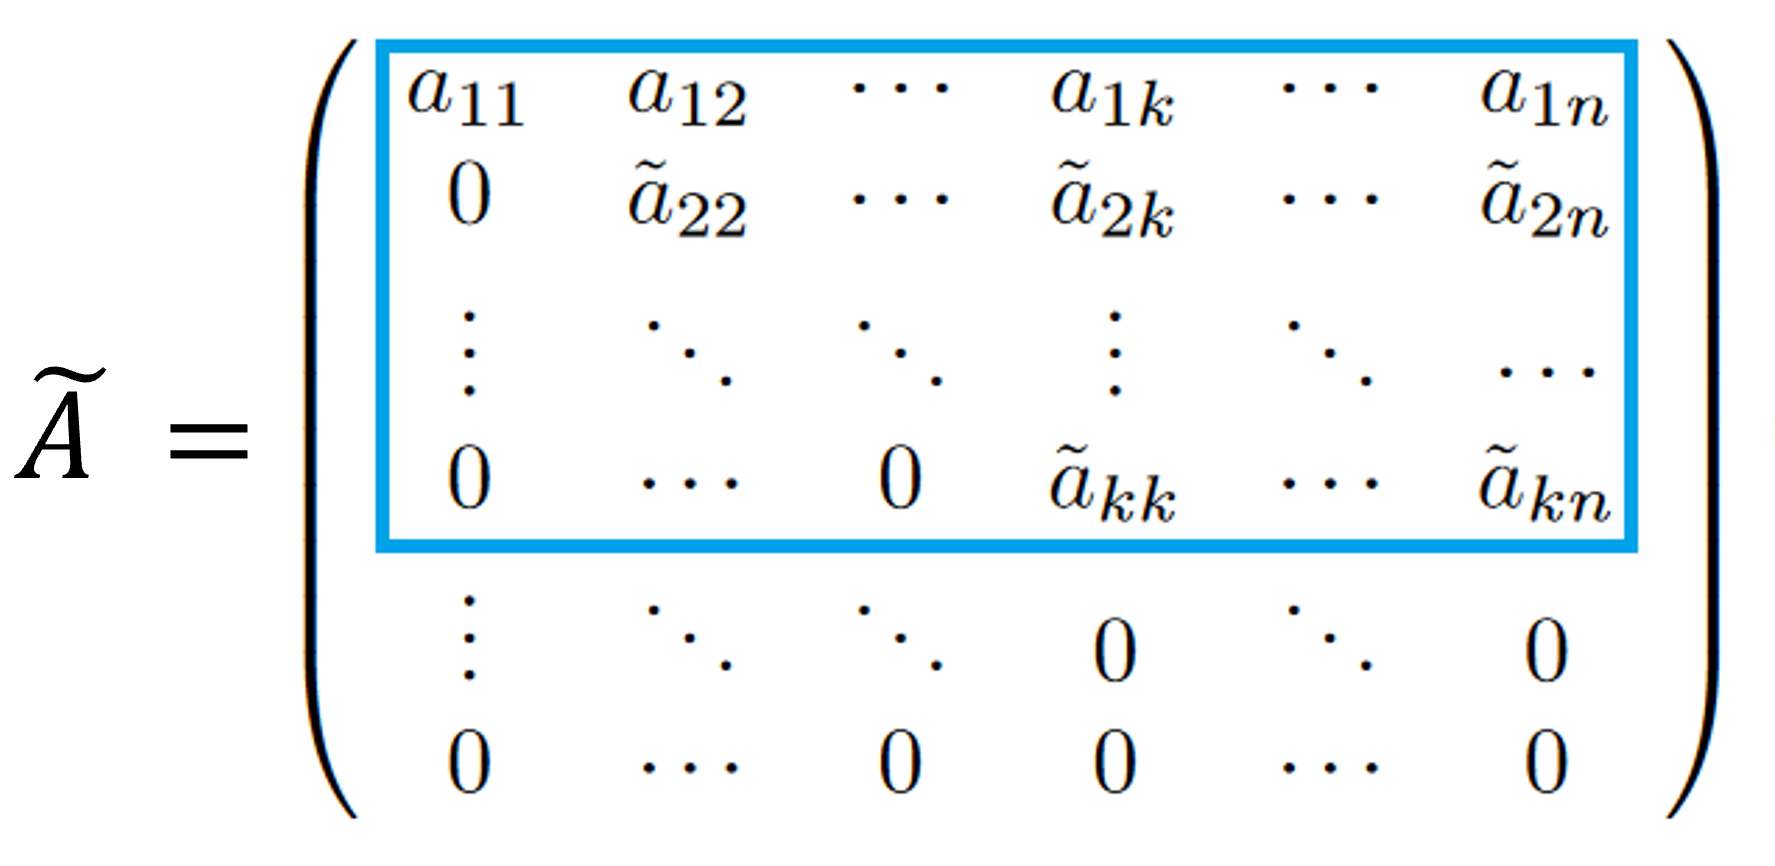
\includegraphics[width=0.4\textwidth]
{../Mathematik_1/Bilder/matrizen_rang_zeilenstufenform.png}
\end{center}

Die Anzahl \(k\) der von Null verschiedenen Zeilen entspricht der Anzahl
der Pivotpositionen und damit dem Rang der Matrix:
\[
\operatorname{rk}(A)=k.
\]

Der zuvor abstrakt als Dimension des Bildes definierte Rang kann damit
mithilfe des Gau�schen Eliminationsverfahrens konkret bestimmt werden.


\subsubsection*{Kern und Defekt bestimmen}

Der Kern einer Matrix wurde definiert durch
\[
\ker(A)
=
\{\vec x\in\mathbb R^n:A\vec x=\vec0\}.
\]

Die Bestimmung des Kerns ist damit nichts anderes als das L�sen des
homogenen linearen Gleichungssystems
\[
A\vec x=\vec0.
\]

Wird \(A\) in Zeilenstufenform gebracht und besitzt die Matrix den Rang
\(k\), so gibt es \(k\) Pivotvariablen. Die �brigen \(n-k\) Variablen sind
freie Variablen.

\begin{center}
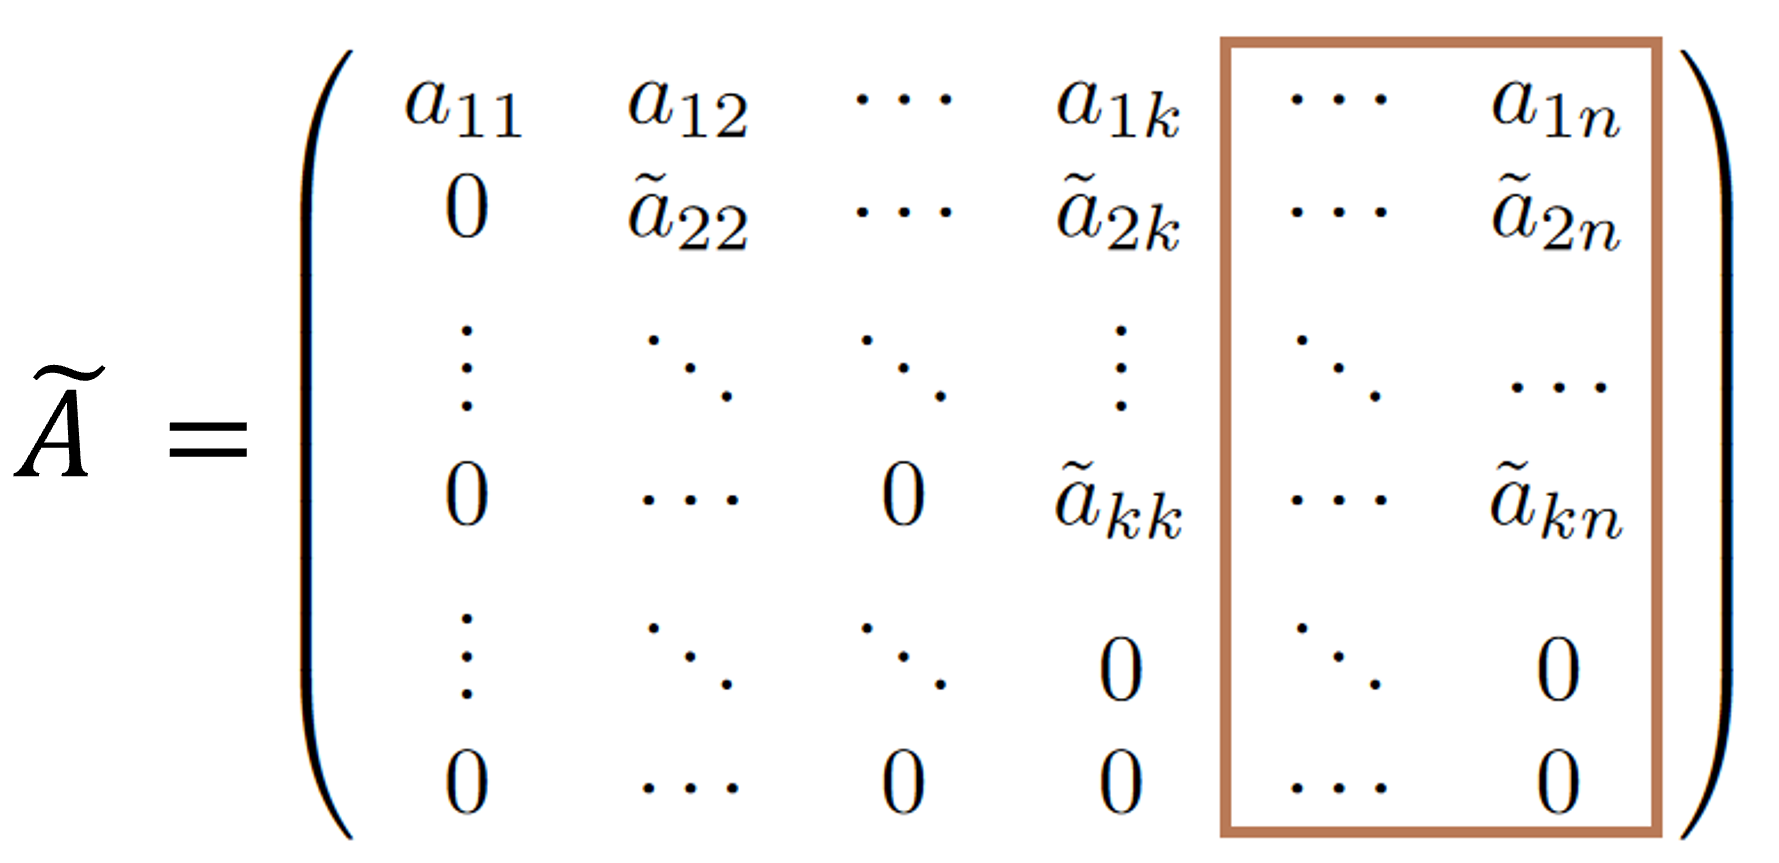
\includegraphics[width=0.4\textwidth]
{../Mathematik_1/Bilder/matrizen_defekt_freie_variablen.png}
\end{center}

Jede freie Variable liefert einen freien Parameter in der allgemeinen
L�sung des homogenen Gleichungssystems. Die Anzahl dieser freien Parameter
entspricht der Dimension des Kerns. Damit gilt
\[
\operatorname{def}(A)
=
\dim\bigl(\ker(A)\bigr)
=
n-k.
\]

Da gleichzeitig
\[
\operatorname{rk}(A)=k
\]
gilt, folgt
\[
\operatorname{rk}(A)+\operatorname{def}(A)=n.
\]

Der Rangsatz erh�lt damit eine unmittelbar sichtbare Bedeutung: Die
\(n\) Variablen zerfallen in \(k\) durch Pivotpositionen bestimmte
Variablen und \(n-k\) freie Variablen. Die Anzahl der freien Parameter
entspricht der Dimension des Kerns.

\subsubsection*{Lineare Unabh�ngigkeit systematisch untersuchen}

Auch die Frage nach der linearen Unabh�ngigkeit mehrerer Vektoren l�sst sich auf ein lineares Gleichungssystem zur�ckf�hren.

Gegeben seien
\[
\vec a_1,\ldots,\vec a_n\in\mathbb R^m.
\]
Nach der Definition sind diese Vektoren genau dann linear unabh�ngig, wenn
aus
\[
x_1\vec a_1+\cdots+x_n\vec a_n=\vec0
\]
notwendig
\[
x_1=\cdots=x_n=0
\]
folgt.

Werden die Vektoren als Spalten einer Matrix
\[
A=
\begin{pmatrix}
\vert&&\vert\\
\vec a_1&\cdots&\vec a_n\\
\vert&&\vert
\end{pmatrix}
\]
angeordnet, so wird die Bedingung zur Matrixgleichung
\[
A\vec x=\vec0.
\]

Damit gilt:
\[
\vec a_1,\ldots,\vec a_n
\text{ sind linear unabh�ngig}
\quad\Longleftrightarrow\quad
\ker(A)=\{\vec0\}.
\]

Die abstrakte Frage nach linearer Unabh�ngigkeit wird dadurch zu einer konkreten Rechenaufgabe: Das zugeh�rige homogene lineare Gleichungssystem wird mit dem Gau�schen Eliminationsverfahren gel�st.

Besitzt es nur die triviale L�sung, sind die Vektoren linear unabh�ngig.  Treten freie Parameter und damit nichttriviale L�sungen auf, sind die Vektoren linear abh�ngig.
\subsubsection*{Das Bild und eine Basis des Bildes bestimmen (+)}

Die Spalten einer Matrix
\[
A=
\begin{pmatrix}
\vert && \vert\\
\vec a_1&\cdots&\vec a_n\\
\vert && \vert
\end{pmatrix}
\]
spannen das Bild der zugeh�rigen linearen Abbildung auf:
\[
\operatorname{im}(A)
=
\operatorname{span}\{\vec a_1,\ldots,\vec a_n\}.
\]

Damit bilden die Spalten von \(A\) zun�chst ein Erzeugendensystem des
Bildes. Dieses Erzeugendensystem muss jedoch nicht linear unabh�ngig sein.
F�r eine Basis des Bildes werden daher gerade so viele linear unabh�ngige
Vektoren ben�tigt, wie der Rang der Matrix angibt.

Das Gau�sche Eliminationsverfahren kann auch verwendet werden, um solche
Basisvektoren systematisch zu bestimmen. Dabei ist zu beachten, dass die
gesuchten Vektoren als \emph{Spalten} in \(A\) stehen, w�hrend das
Gau�verfahren mit \emph{Zeilen} arbeitet.

Deshalb wird zun�chst die transponierte Matrix
\[
A^{\intercal}
\]
gebildet. Die Spaltenvektoren von \(A\) erscheinen darin als Zeilenvektoren.
Anschlie�end wird \(A^{\intercal}\) durch elementare Zeilenumformungen in
Zeilenstufenform �berf�hrt \(A^\intercal \longrightarrow \widetilde{ ( A^\intercal) } \).

\begin{center}
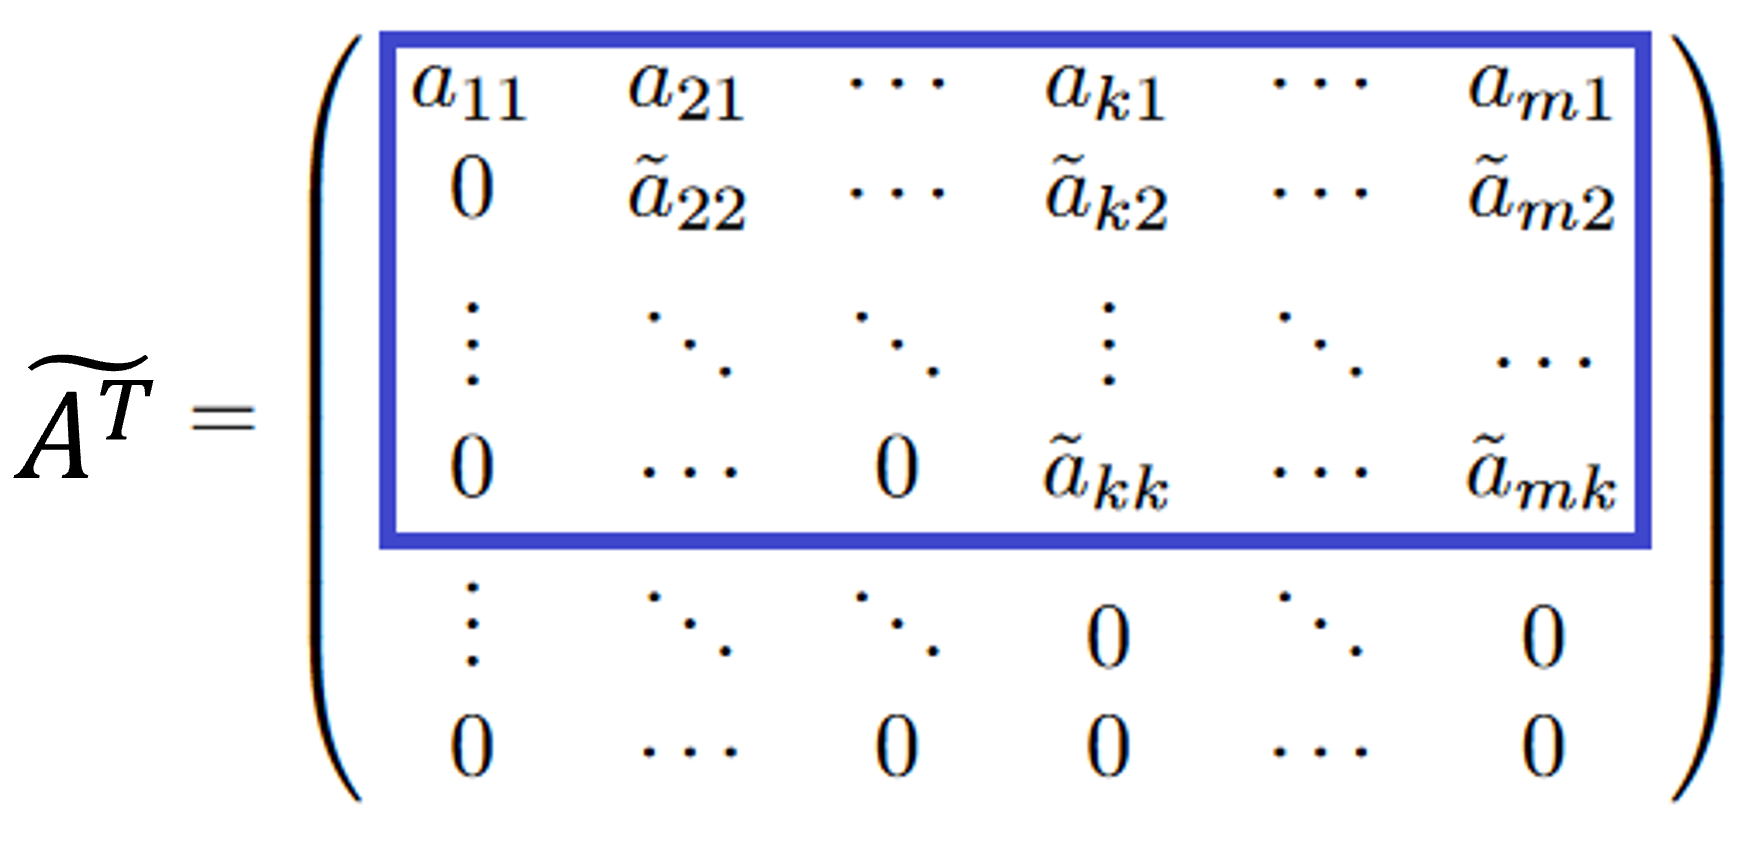
\includegraphics[width=0.4\textwidth]
{../Mathematik_1/Bilder/matrizen_bildbasis_transponierte_zeilenstufenform.png}
\end{center}

Die elementaren Zeilenumformungen ver�ndern den von den Zeilen aufgespannten
Vektorraum nicht. In der Zeilenstufenform bleiben daher genau \(k\)
linear unabh�ngige Nichtnullzeilen �brig, wenn
\[
\operatorname{rk}(A)=k.
\]

Diese \(k\) Zeilen bilden eine Basis des Zeilenraums von
\(A^{\intercal}\). Durch erneutes Transponieren werden daraus
Spaltenvektoren in \(\mathbb R^m\). Diese Vektoren bilden eine Basis des
Bildes von \(A\).

Damit liefert das Gau�sche Eliminationsverfahren nicht nur die Dimension
des Bildes. Durch die Anwendung auf die transponierte Matrix k�nnen auch
konkrete Basisvektoren des Bildes bestimmt werden.


\subsubsection*{Eine gemeinsame Systematik}

Mehrere zuvor getrennt eingef�hrte Begriffe lassen sich damit auf dieselbe Rechenmethode zur�ckf�hren:

\[
A\vec x=\vec b
\quad\longrightarrow\quad
\text{L�sbarkeit und L�sungsmenge},
\]

\[
A\vec x=\vec0
\quad\longrightarrow\quad
\text{Kern und Defekt},
\]

und die Zeilenstufenform von \(A\) liefert Informationen �ber Rang, Pivotspalten und damit �ber lineare Unabh�ngigkeit und eine Basis des Bildes.

Das Gau�sche Eliminationsverfahren ist deshalb nicht nur ein Verfahren zum L�sen linearer Gleichungssysteme. Es ist ein grundlegendes Rechenwerkzeug der linearen Algebra, das die abstrakten Begriffe der vorangegangenen Abschnitte konkret zug�nglich macht.


%----------------------------------------------------------
\subsection*{Ausblick}

�berbestimmte Gleichungssysteme m�ssen nicht l�sbar sein. In vielen Anwendungen entsteht dann die Frage, ob zumindest ein Vektor gefunden werden kann, der die Gleichungen m�glichst gut erf�llt. Dies f�hrt zur \textbf{Methode der kleinsten Fehlerquadrate} (\emph{least squares}), die beispielsweise bei der linearen Regression eine
zentrale Rolle spielt.

Das Gau�sche Eliminationsverfahren ist ein \textbf{direktes L�sungsverfahren}. Bei exakter Arithmetik wird nach endlich vielen Eliminationsschritten eine Form erreicht, aus der sich die L�sungsstruktur bestimmen l�sst. Bei numerischen Rechnungen mit Gleitkommazahlen kommen zus�tzlich Rundungsfehler und Fragen der numerischen Stabilit�t hinzu.

F�r sehr gro�e lineare Gleichungssysteme k�nnen dagegen \textbf{iterative Verfahren} (\emph{iterative methods}) zweckm��ig sein.  Dabei wird ausgehend von einem Startwert eine Folge von N�herungen erzeugt, die unter geeigneten Voraussetzungen gegen die gesuchte L�sung konvergiert.

Ein grundlegendes Beispiel ist das \textbf{Jacobi-Verfahren} (\emph{Jacobi method}). F�r bestimmte Klassen quadratischer Matrizen konvergiert dieses Verfahren zur L�sung des Gleichungssystems. Eine hinreichende Bedingung ist beispielsweise strikte Diagonaldominanz der Matrix. Die Untersuchung solcher Verfahren und ihrer Konvergenzeigenschaften geh�rt zur numerischen Mathematik.

 \newpage % Lineare Gleichungssysteme
\setcounter{exercise}{0} 	
\ifintegriereaufgaben
\section*{Lineare Gleichungssysteme Aufgaben}\label{MA1-lineare-gleichungssysteme-aufgaben}

	Regeln und Beispiele, die zur Bearbeitung der Aufgaben hilfreich sind, finden Sie im Skript\wennreferenzvorhanden{MA1-lineare-gleichungssysteme}{ (Abschnitt \abschnittsverweis{MA1-lineare-gleichungssysteme})} und, falls Sie nicht weiterkommen, schauen Sie \hyperref[MA1-lineare-gleichungssysteme-loesungen]{hier}.
\else
\section{Lineare Gleichungssysteme Aufgaben}\label{MA1-lineare-gleichungssysteme-aufgaben}

	Regeln und Beispiele, die zur Bearbeitung der Aufgaben hilfreich sind, finden Sie im Skript und, falls Sie nicht weiterkommen, schauen Sie \hyperref[MA1-lineare-gleichungssysteme-loesungen]{hier}.

\fi 

\begin{exercisebox}[Rechenregeln]
	Wie muss $\boldsymbol b$ gew�hlt werden, dass gilt $A\boldsymbol x =\boldsymbol b$ mit \[ \left( \begin{array}{ccccc} -1 & 0 & 0 & 3 & -2 \\  2 & -1 & 1 & 0 & 0 \\ 1 & 1 & -1 & -2 & 0 \end{array}\right), \quad \boldsymbol x = \left( -1, 2,-2,3,5\right)^\intercal\,.\]
\end{exercisebox}

\begin{exercisebox}[L�sbarkeitsanalyse]
	Gegeben seien \[ A = \left( \begin{array}{cc} 1 & 1 \\ 2 & \alpha \end{array}\right), \quad \boldsymbol b = \left( \begin{array}{c} -2 \\ \beta \end{array}\right)\] mit Parametern $\alpha, \beta\in \mathbb R$. 
	\begin{itemize}
		\item[(a)] Bestimmen Sie den Rang der Matrix $A$ in Abh�ngigkeit von $\alpha$.
		\item[(b)] Bestimmen Sie den Rang der erweiterten Matrix $(A|b)$ in Abh�ngigkeit von $\alpha$ und $\beta$.
		\item[(c)] Bestimmen Sie in Abh�ngigkeit der beiden Parameter, wann das lineare Gleichugnssystem $A\boldsymbol x = \boldsymbol b$ l�sbar ist und wann es genau eine L�sung gibt.
	\end{itemize}
\end{exercisebox}

\begin{exercisebox}[Gleichungssysteme]
	Analysieren Sie die L�sbarkeit der folgenden Gleichungssysteme und bestimmen Sie die L�sungsmenge:
	\begin{eqnarray*}
		\begin{array}{ll} 
			(a) \; \begin{cases}
				x_1 -x_2 - x_3 &= 0\\
				x_1 +x_2 + 3x_3 &= 4\\
				     x_2 + 2x_3 &= 2\\
				     2x_1 + x_3 &= 3\\
    \end{cases} 
   &\quad  
    (b)\; \begin{cases}
	    x_1 + x_2 - x_3 + x_4 - x_5 &= 1\\
    -x_1 + x_2 - 3 x_3 + 3x_5 &= 2\\
    x_2 - 2 x_3 + x_4 - x_5 &= -1\\
    2x_1 + 2 x_3 + x_4 - 2 x_5 &= 1
  \end{cases} \\[3ex]
  (c)\; \begin{cases}
	x_1 + x_2 - x_3 &=1 \\
	2x_1 + 3x_2 + px_3 &= 3 \\
	x_1 + px_2 + 3x_3 &= 2
    \end{cases}   
   &\quad  
	(d)\; \begin{cases}
    3x_1 + x_2-4x_3 &= 2\\
    x_1 + x_2&= 0\\
    4x_1 +5x_3 + x_4 &= 1 \\
    6x_2 +x_3 + 2x_4 &= 1
  \end{cases} \\[3ex]
  (e)\;\begin{cases}
	  (2+i)\cdot z_1 + i\cdot z_3 &= -4+3i \\ 
		(1+3i)\cdot z_1 + (-1-i)\cdot z_2  - z_3 &= -6-2i \\ 
		(4+2i)\cdot z_2 + (3+3i)\cdot z_3 &= -2+4i 
	\end{cases} 
  \end{array}
   &\quad  
  \end{eqnarray*}

  \end{exercisebox}

\begin{exercisebox}[Gleichungssysteme]
	Gesucht ist eine Matrix $X\in \mathbb R^{2\times 2}$ so, dass \[ A X + X A^\intercal = C, \quad A=\left( \begin{array}{cc} 1 & -1 \\ 2 & 2 \end{array}\right), \; C = \left( \begin{array}{cc} 4 & 0 \\ 6 & 4 \end{array}\right) \,. \]
	Bestimmen Sie ein lineares Gleichungssystem f�r die unbekannten Koeffizienten $x_{ij},\; i,j=1,2$ der Matrix $X$ und l�sen Sie es.
  \end{exercisebox}

%\begin{exabox}[�berbestimmtes Gleichungssystem]
%	Bestimme die Normalform einer Ebene, wenn die Ebene durch drei Punkte festgelegt ist. 
%  \begin{eqnarray*}
%	  \boldsymbol w = \left( \begin{array}{c} u_2 v_3 - u_3 v_2 \\ u_3 v_1 - u_1 v_3 \\u_1 v_2 - u_2 v_1\end{array}\right) 
%  \end{eqnarray*}
%\end{exabox}

%\begin{exabox}[Analytische Geometrie]
%	Lineares Gleichungssystem l�sen zur expliziten Ebenengleichung bei gegebenen drei Punkten.  - Sp�ter noch mit Determinante?
%\end{exabox}

%\begin{exabox}[Kreuzprodukt] 
%	Geben Sie alle Vektoren $\boldsymbol b\in\mathbb R^3$ an, so dass folgende Bedingungen gelten: 
%	\[ \boldsymbol e_1 \times \boldsymbol b = \boldsymbol e_3, \quad \boldsymbol b \perp \left( \begin{array}{c} 1 \\1 \\ 1\end{array}\right)\,, \] wobei $\boldsymbol e_i$ den $i$-ten Einheitsvektor bezeichnet. Hinweis: Machen Sie hierf�r den Ansatz $\boldsymbol b = \left( b_1, b_2, b_3\right)^\intercal$ und bestimmen Sie ein lineares Gleichungsystem.
%\end{exercisebox}

%\begin{exercisebox}[Direkte Verfahren: bringe auf Dreiecksform]
%	\begin{itemize}
%		\item Gau�sches Eliminationsverfahren 
%		\item Givens-Rotationen
%		\item Householderverfahren
%		\item Cholesky-Zerlegung (positive definite Matrix)
%	\end{itemize}
%\end{exercisebox}
%
%\begin{exercisebox}[Direkte Verfahren, numerischer Aufwand]
%\end{exercisebox}
%
%\begin{exercisebox}[LU-Zerlegung, numerischer Aufwand]
%\end{exercisebox}
%
%\begin{exercisebox}[LR-Zerlegung, numerischer Aufwand]
%\end{exercisebox}
%
%\begin{exercisebox}[Beispiel Matrix aufstellen]
%\end{exercisebox}
%
%\begin{theorembox}[Iterative Methoden - GC-Verfahren, numerischer Aufwand]
%\end{theorembox}
%
%\begin{theorembox}[Iterative Methoden - GMRES, numerischer Aufwand]
%\end{theorembox}
%
%\begin{theorembox}[Norm einer Matrix]
%\end{theorembox}
%
%\begin{exercisebox}[Konditionszahl]
%\end{exercisebox}
%
%\begin{exercisebox}[Vorkonditionierung]
%\end{exercisebox}
%
%\begin{theorembox}[Parallelisierung von Prozessen]
%\end{theorembox}
%
%\begin{exercisebox}[Mathematik lesen, keine eindeutige L�sung]
%\end{exercisebox}
%
%\begin{theorembox}[Rang - MC]
%	\begin{itemize}
%		\item Der Rang der Matrix $A$ ist die Anzahl der nichttrivialen Zeilen in ihrer Zeilennormalform. 
%		\item Der Rang der Matrix $A$ ist die Anzahl der linear unabh�ngigen Spalten. 
%		\item Der Rang der Matrix $A$ ist die Anzahl der linear unabh�ngigen Zeilen. 
%		\item Der Rang einer Matrix ist die Dimension des Bildes. 
%	\end{itemize}
%\end{theorembox}
%
%\begin{theorembox}[Fredholmsche Alternative - Beweis vorf�hren bitte]
%  Entweder $A\boldsymbol x = b$ ist eindeutig l�sbar f�r alle $\boldsymbol b \in \mathbb R^n$ oder $A\boldsymbol x = \boldsymbol 0$ hat eine nichttriviale L�sung. 
%  \[ \Rightarrow A\boldsymbol x = \boldsymbol b \textnormal{ eindeutig f�r alle } \boldsymbol b\in\mathbb R^n, \textnormal{ d.h. } A\boldsymbol x = 0 \textnormal{ eindeutig l�sbar, d.h. } \mathrm{ker}A = \{\boldsymbol 0\}\]
%  \[ \Leftarrow \mathrm{ker}A = \{\boldsymbol 0\}, \textnormal{ so folgt } \mathrm{def}A = 0 \Rightarrow \mathrm{rk}A = n \Rightarrow \textnormal{ eindeutige L�sung}\,. \]
%\end{theorembox}

 \newpage 
\setcounter{satz}{0} \setcounter{def}{0} \setcounter{exa}{0}  
\section{Determinante und Inverse (+)}\label{MA1-determinante-und-inverse}

\begin{table}[H]
  \centering
  \begin{tabularx}{\textwidth}{p{0.9\textwidth} p{0.1\textwidth}}
    \toprule
    \multicolumn{2}{c}{\textbf{�bersicht �ber Lernziele und Voraussetzungen}}\\
    \midrule
    \textbf{Lernziele} &\\[.5\normalbaselineskip]
    \tabitem die Determinante einer quadratischen Matrix berechnen und geometrisch interpretieren &\\
    \tabitem den Zusammenhang zwischen Determinante, Rang und Invertierbarkeit erl�utern &\\
    \tabitem die Bedeutung der inversen Matrix als Darstellung der Umkehrabbildung erkl�ren &\\
    \tabitem die inverse Matrix zur L�sung linearer Gleichungssysteme interpretieren &\\
    \midrule
    \textbf{Voraussetzungen} &\\[.5\normalbaselineskip]
    \tabitem Umkehrfunktion & \abschnittsverweis{MA1-eigenschaften-von-funktionen}\\
    \tabitem Rang und Defekt einer Matrix & \abschnittsverweis{MA1-matrizen}\\
    \tabitem Gau�sches Eliminationsverfahren & \abschnittsverweis{MA1-lineare-gleichungssysteme}\\
    \bottomrule
  \end{tabularx}
\end{table}

\ifintegriereaufgaben
\noindent �bungsaufgaben zum Thema finden sich hier:
\hyperref[MA1-determinante-und-inverse-aufgaben]{Aufgaben}
\vspace{0.3cm}
\hrule
\fi


\subsection{Was ist die Determinante?}

Eine quadratische Matrix
\[
A\in\mathbb R^{n\times n}
\]
beschreibt eine lineare Abbildung
\[
\mathcal A:\mathbb R^n\to\mathbb R^n,
\qquad
\vec x\mapsto A\vec x.
\]
Eine solche Abbildung kann den Raum beispielsweise strecken, stauchen,
scheren oder spiegeln. Dabei ver�ndert sie im Allgemeinen auch Fl�chen
beziehungsweise Volumina.

Die \textbf{Determinante} (\emph{determinant}) ordnet jeder quadratischen
Matrix eine reelle Zahl zu:
\begin{defbox}{Determinante}{ }
\[
\det:\mathbb R^{n\times n}\to\mathbb R,
\qquad
A\mapsto\det(A).
\]
\end{defbox}

Diese zun�chst abstrakt erscheinende Zahl besitzt eine anschauliche
geometrische Bedeutung. Sie beschreibt, wie die zu \(A\) geh�rende lineare
Abbildung orientierte Volumina ver�ndert.

\begin{defbox}{Geometrische Bedeutung der Determinante}{ }
\begin{itemize}
    \item Der Betrag \(|\det(A)|\) gibt an, um welchen Faktor
    \(n\)-dimensionale Volumina durch die lineare Abbildung ver�ndert
    werden. F�r \(n=2\) sind dies Fl�cheninhalte, f�r \(n=3\) Volumina.

    \item Das Vorzeichen der Determinante beschreibt, ob die Orientierung
    erhalten bleibt oder umgekehrt wird.

    \item F�r \(\det(A)=0\) wird das \(n\)-dimensionale Volumen vollst�ndig
    auf null zusammengedr�ckt. Das Bild der linearen Abbildung besitzt dann
    eine kleinere Dimension als der Ausgangsraum.
\end{itemize}

\begin{center}
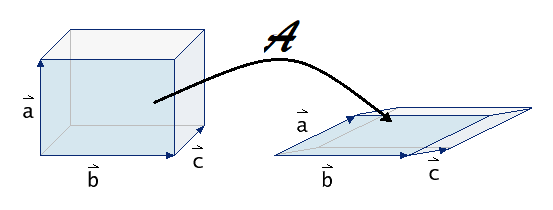
\includegraphics[width=0.6\textwidth]
{../Mathematik_1/Bilder/determinante_volumenverlust_dimension.png}
\end{center}
\end{defbox}

Gerade der letzte Fall wird sp�ter eine besondere Bedeutung erhalten:
Wenn \(\det(A)=0\) gilt, geht durch die lineare Abbildung mindestens eine
Raumrichtung verloren. Die Abbildung kann dann nicht umkehrbar sein.

F�r einfache geometrische Transformationen
\[
\mathcal A:\mathbb R^2\to\mathbb R^2,
\qquad
\vec x\mapsto A\vec x,
\]
l�sst sich die Determinante bereits aus der geometrischen Wirkung der
Abbildung verstehen.

\begin{exabox}{Determinanten f�r einfache geometrische Transformationen}{ }
\begin{eqnarray*}
\left| \begin{array}{cc} 0 & 0 \\ 0 & 0 \end{array}\right|
&=&0\,,
\quad \textnormal{Nullabbildung},\\
\left| \begin{array}{cc} 1 & 0 \\ 0 & 1 \end{array}\right|
&=&1\,,
\quad \textnormal{Identit�tsabbildung},\\
\left| \begin{array}{cc} 2 & 0 \\ 0 & 2 \end{array}\right|
&=&4\,,
\quad \textnormal{Skalierung in zwei Richtungen},\\
\left| \begin{array}{cc} 2 & 0 \\ 0 & 1 \end{array}\right|
&=&2\,,
\quad \textnormal{Skalierung in einer Koordinatenrichtung},\\
\left| \begin{array}{cc}
\frac{1}{\sqrt{2}} &-\frac{1}{\sqrt{2}}\\
\frac{1}{\sqrt{2}} & \frac{1}{\sqrt{2}}
\end{array}\right|
&=&1\,,
\quad \textnormal{Drehung},\\
\left| \begin{array}{cc} 0&1\\1&0\end{array}\right|
&=&-1\,,
\quad \textnormal{Spiegelung},\\
\left| \begin{array}{cc}1&1\\0&1\end{array}\right|
&=&1\,,
\quad \textnormal{Scherung in einer Achsenrichtung}.
\end{eqnarray*}
\end{exabox}

Die Beispiele zeigen bereits zwei unterschiedliche Informationen der
Determinante. Eine Drehung und eine Scherung k�nnen den Fl�cheninhalt
unver�ndert lassen und besitzen daher den Betrag \(1\). Eine Spiegelung
l�sst den Fl�cheninhalt ebenfalls unver�ndert, kehrt jedoch die Orientierung
um und besitzt deshalb eine negative Determinante.


\subsection{Eigenschaften und Berechnung der Determinante}

Werden zwei lineare Abbildungen hintereinander ausgef�hrt, so
multiplizieren sich ihre Volumenskalierungsfaktoren. Entsprechend gilt f�r
quadratische Matrizen \(A\) und \(B\):

\begin{theorembox}{Determinante eines Produkts}{ }
\[
\det(AB)=\det(A)\cdot\det(B).
\]
\end{theorembox}

Hieraus und aus den grundlegenden Eigenschaften der Determinante ergeben
sich Rechenregeln f�r Ver�nderungen einzelner Spalten beziehungsweise
Zeilen.

\begin{exabox}{Rechenregeln}{ }
\begin{enumerate}

\item Wird eine Spalte oder Zeile mit einem Faktor \(\lambda\)
multipliziert, so wird auch die Determinante mit \(\lambda\) multipliziert:
\begin{eqnarray*}
\left| \begin{array}{ccc}
2&-7&\textcolor{blue}{3}\\
0&2&\textcolor{blue}{6}\\
4&1&\textcolor{blue}{9}
\end{array}\right|
=
\textcolor{blue}{3}
\left| \begin{array}{ccc}
2&-7&1\\
0&2&2\\
4&1&3
\end{array}\right|.
\end{eqnarray*}

\item Werden zwei Spalten oder Zeilen vertauscht, so wechselt das
Vorzeichen der Determinante:
\begin{eqnarray*}
\left| \begin{array}{ccc}
2&\textcolor{blue}{-7}&\textcolor{brown}{3}\\
0&\textcolor{blue}{2}&\textcolor{brown}{6}\\
4&\textcolor{blue}{1}&\textcolor{brown}{9}
\end{array}\right|
=
-
\left| \begin{array}{ccc}
2&\textcolor{brown}{3}&\textcolor{blue}{-7}\\
0&\textcolor{brown}{6}&\textcolor{blue}{2}\\
4&\textcolor{brown}{9}&\textcolor{blue}{1}
\end{array}\right|.
\end{eqnarray*}

\item Besitzt eine Matrix zwei identische Spalten oder Zeilen, so
verschwindet ihre Determinante:
\begin{eqnarray*}
\alpha
&=&
\left| \begin{array}{ccc}
\textcolor{blue}{2}&-7&\textcolor{brown}{2}\\
\textcolor{blue}{0}&2&\textcolor{brown}{0}\\
\textcolor{blue}{4}&1&\textcolor{brown}{4}
\end{array}\right| \\
&=&
-
\left| \begin{array}{ccc}
\textcolor{brown}{2}&-7&\textcolor{blue}{2}\\
\textcolor{brown}{0}&2&\textcolor{blue}{0}\\
\textcolor{brown}{4}&1&\textcolor{blue}{4}
\end{array}\right|
=-\alpha,
\end{eqnarray*}
also \(\alpha=0\).

\item Die Determinante ist in jeder einzelnen Spalte beziehungsweise Zeile
linear. Ist beispielsweise eine Spalte die Summe zweier Vektoren, so kann
die Determinante entsprechend zerlegt werden:
\begin{eqnarray*}
\left| \begin{array}{cc}2&2\\3&5\end{array}\right|
&=&
\left| \begin{array}{cc}\textcolor{blue}{2+}0&2\\
\textcolor{blue}{1+}2&5\end{array}\right|\\
&=&
\left| \begin{array}{cc}\textcolor{blue}{2}&2\\
\textcolor{blue}{1}&5\end{array}\right|
\textcolor{blue}{+}
\left| \begin{array}{cc}0&2\\2&5\end{array}\right|.
\end{eqnarray*}

\item Wird zu einer Spalte oder Zeile ein Vielfaches einer anderen Spalte
beziehungsweise Zeile addiert, so ver�ndert sich die Determinante nicht.
Diese Eigenschaft ist insbesondere bei der Berechnung von Determinanten
mithilfe des Gau�schen Eliminationsverfahrens n�tzlich.

\end{enumerate}
\end{exabox}

\noindent\textbf{Bemerkungen:}
\begin{itemize}
    \item Es gilt
    \[
    \det(A)=\det(A^\intercal).
    \]
    Daher gelten die entsprechenden Rechenregeln gleicherma�en f�r
    Spalten und Zeilen.

    \item Die Determinante ist in ihren Spalten beziehungsweise Zeilen
    multilinear und alternierend. Insbesondere verschwindet sie, sobald
    zwei Spalten beziehungsweise zwei Zeilen identisch sind.
\end{itemize}


\subsubsection*{Determinante einer \(2\times2\)-Matrix}

Die Rechenregeln erm�glichen nun die Berechnung konkreter Determinanten.
F�r eine \(2\times2\)-Matrix ergibt sich beispielsweise
\begin{eqnarray*}
\left| \begin{array}{cc}
\textcolor{blue}{1}&\textcolor{brown}{2}\\
\textcolor{brown}{3}&\textcolor{blue}{4}
\end{array}\right|
&=&
\textcolor{blue}{1}\cdot\textcolor{blue}{4}
-
\textcolor{brown}{2}\cdot\textcolor{brown}{3}\\
&=&-2.
\end{eqnarray*}

Allgemein gilt damit:

\begin{defbox}{Determinante einer \(2\times2\)-Matrix}{ }
\[
\left|
\begin{array}{cc}
\textcolor{blue}{a}&\textcolor{brown}{b}\\
\textcolor{brown}{c}&\textcolor{blue}{d}
\end{array}
\right|
=
\textcolor{blue}{a}\cdot\textcolor{blue}{d}
-
\textcolor{brown}{b}\cdot\textcolor{brown}{c}.
\]
\end{defbox}


\subsubsection*{Entwicklung einer \(3\times3\)-Determinante}

Eine \(3\times3\)-Determinante kann auf \(2\times2\)-Determinanten
zur�ckgef�hrt werden. Bei einer Entwicklung nach der ersten Spalte ergibt
sich beispielsweise

\begin{exabox}{Entwicklung nach der ersten Spalte}{ }
\begin{eqnarray*}
\left|
\begin{array}{ccc}
\textcolor{blue}{1}&2&3\\
\textcolor{blue}{4}&5&6\\
\textcolor{blue}{7}&8&9
\end{array}
\right|
&=&
\textcolor{blue}{1}
\left|\begin{array}{cc}5&6\\8&9\end{array}\right|
-
\textcolor{blue}{4}
\left|\begin{array}{cc}2&3\\8&9\end{array}\right|
+
\textcolor{blue}{7}
\left|\begin{array}{cc}2&3\\5&6\end{array}\right|\\
&=&
(5\cdot9-6\cdot8)
-4(2\cdot9-3\cdot8)
+7(2\cdot6-3\cdot5)\\
&=&-3+24-21=0.
\end{eqnarray*}
\end{exabox}

Entsprechend kann eine Determinante nach jeder Zeile oder Spalte entwickelt
werden. Das Vorzeichen des jeweiligen Terms h�ngt von seiner Position ab
und folgt dem Schachbrettmuster:

\begin{theorembox}{Vorzeichen im Schachbrettmuster}{ }
\[
\left|
\begin{array}{ccc}
+&-&+\\
-&+&-\\
+&-&+
\end{array}
\right|.
\]
\end{theorembox}

F�r \(3\times3\)-Determinanten ergibt sich au�erdem die leicht zu merkende
\textbf{Regel von Sarrus}:

\begin{eqnarray*}
\left|
\begin{array}{ccc}
1&2&3\\
4&5&6\\
7&8&9
\end{array}
\right|
\textcolor{lightgray}{
\begin{array}{cc}
1&2\\4&5\\7&8
\end{array}}
=
\textcolor{red}{1\cdot5\cdot9+2\cdot6\cdot7+3\cdot4\cdot8}
\textcolor{blue}{-7\cdot5\cdot3-8\cdot6\cdot1-9\cdot4\cdot2}.
\end{eqnarray*}

Die Regel von Sarrus gilt ausschlie�lich f�r \(3\times3\)-Matrizen. Sie
l�sst sich nicht auf Determinanten der Gr��e \(4\times4\) oder h�her
�bertragen.

Bei einer direkten Entwicklung einer \(n\times n\)-Determinante entstehen
\(n!\) Produkte mit jeweils \(n\) Faktoren. Der Rechenaufwand w�chst daher
sehr schnell. F�r gr��ere Matrizen ist eine vollst�ndige Entwicklung
deshalb kein zweckm��iges Berechnungsverfahren.

Eine Alternative ergibt sich aus dem bereits bekannten Gau�schen
Eliminationsverfahren. Wird eine Matrix unter Beachtung der oben
angegebenen Rechenregeln auf Dreiecksgestalt gebracht, so l�sst sich die
Determinante anschlie�end unmittelbar aus den Diagonaleintr�gen bestimmen.
F�r eine Dreiecksmatrix gilt
\[
\det(A)=a_{11}a_{22}\cdots a_{nn}.
\]


\subsubsection*{Das Spatprodukt (+)}

Mit der Determinante l�sst sich eine weitere geometrische Verkn�pfung von
Vektoren beschreiben. Das \textbf{Spatprodukt} (\emph{triple product}) ist
eine Besonderheit des \(\mathbb R^3\) und bildet drei Vektoren auf eine
reelle Zahl ab.

Sind \(\vec x_1,\vec x_2,\vec x_3\in\mathbb R^3\), so werden diese als
Spalten einer Matrix zusammengefasst:

\begin{defbox}{Spatprodukt}{ }
\[
\mathbb R^3\times\mathbb R^3\times\mathbb R^3\to\mathbb R,
\qquad
(\vec x_1,\vec x_2,\vec x_3)
\mapsto
\det(\vec x_1,\vec x_2,\vec x_3).
\]
\end{defbox}

Beispielsweise gilt

\begin{exabox}{Spatprodukt}{ }
\[
\left|
\begin{array}{ccc}
1&3&4\\
2&0&-2\\
3&2&1
\end{array}
\right|
=-4.
\]
\end{exabox}

Der Betrag des Spatprodukts liefert das Volumen des von den drei Vektoren
aufgespannten Parallelepipeds. Das Vorzeichen beschreibt zus�tzlich die
Orientierung der drei Vektoren.


\subsection{Inverse Matrix}

F�r ein quadratisches lineares Gleichungssystem
\[
A\vec x=\vec b,
\qquad
A\in\mathbb R^{n\times n},
\]
wurde im vorangegangenen Abschnitt gezeigt, dass die L�sbarkeit und
Eindeutigkeit der L�sung eng mit Rang und Kern der Koeffizientenmatrix
zusammenh�ngen.

F�r quadratische Matrizen liefert die Determinante nun ein besonders
kompaktes Kriterium. Ist
\[
\det(A)=0,
\]
so wird mindestens eine Raumrichtung durch die zugeh�rige lineare Abbildung
verloren. Das Bild besitzt eine Dimension kleiner als \(n\), also
\[
\operatorname{rk}(A)<n.
\]
Die Abbildung kann deshalb nicht bijektiv und damit auch nicht umkehrbar
sein.

Ist dagegen
\[
\det(A)\neq0,
\]
so geht keine Raumrichtung verloren. Die Matrix besitzt vollen Rang,
\[
\operatorname{rk}(A)=n,
\]
und die zugeh�rige lineare Abbildung
\[
\mathcal A:\mathbb R^n\to\mathbb R^n,
\qquad
\vec x\mapsto A\vec x,
\]
ist bijektiv.

Damit sind f�r eine quadratische Matrix mehrere der bisher eingef�hrten
Begriffe unmittelbar miteinander verbunden:

\begin{theorembox}{Determinante und Invertierbarkeit}{ }
F�r \(A\in\mathbb R^{n\times n}\) sind die folgenden Aussagen �quivalent:
\[
\begin{aligned}
\det(A)&\neq0\\
&\Longleftrightarrow\operatorname{rk}(A)=n\\
&\Longleftrightarrow\operatorname{def}(A)=0\\
&\Longleftrightarrow\ker(A)=\{\vec0\}\\
&\Longleftrightarrow\mathcal A:\mathbb R^n\to\mathbb R^n
   \text{ ist bijektiv}\\
&\Longleftrightarrow A\text{ ist invertierbar}.
\end{aligned}
\]
\end{theorembox}

Damit erh�lt die Determinante eine zweite Bedeutung neben ihrer
geometrischen Interpretation: Sie entscheidet bei einer quadratischen
Matrix mit einer einzigen Zahl dar�ber, ob die zugeh�rige lineare Abbildung
umkehrbar ist.


\subsubsection*{Die Inverse als Umkehrabbildung}

Ist \(\det(A)\neq0\), so ist die lineare Abbildung
\[
\mathcal A:\mathbb R^n\to\mathbb R^n,
\qquad
\vec x\mapsto A\vec x,
\]
bijektiv. Zu jedem \(\vec b\in\mathbb R^n\) existiert daher genau ein
\(\vec x\in\mathbb R^n\) mit
\[
A\vec x=\vec b.
\]

Die Umkehrabbildung
\[
\mathcal A^{-1}:\mathbb R^n\to\mathbb R^n
\]
ordnet jedem \(\vec b\) wieder den eindeutig bestimmten Ausgangsvektor
\(\vec x\) zu. Auch diese Umkehrabbildung ist linear und kann deshalb
wieder durch eine Matrix dargestellt werden. Diese Matrix ist die
\textbf{inverse Matrix} (\emph{inverse matrix}) \(A^{-1}\).

\begin{defbox}{Inverse Matrix}{ }
Eine quadratische Matrix \(A\in\mathbb R^{n\times n}\) hei�t
\textbf{invertierbar} (\emph{invertible}), wenn eine Matrix
\(A^{-1}\in\mathbb R^{n\times n}\) existiert mit
\[
A^{-1}A=AA^{-1}=I_n.
\]
Die Matrix \(A^{-1}\) ist die Matrixdarstellung der Umkehrabbildung
\(\mathcal A^{-1}\).
\end{defbox}

Die Schreibweise \(A^{-1}\) erinnert bewusst an den Kehrwert einer Zahl.
F�r eine Zahl \(a\neq0\) gilt
\[
a^{-1}a=aa^{-1}=1.
\]
Bei einer invertierbaren Matrix �bernimmt die Einheitsmatrix \(I_n\) die
Rolle der Zahl \(1\):
\[
A^{-1}A=AA^{-1}=I_n.
\]

Der entscheidende Unterschied zu einer einzelnen L�sung eines linearen
Gleichungssystems besteht darin, dass \(A^{-1}\) nur von der Matrix \(A\)
und nicht von der rechten Seite \(\vec b\) abh�ngt.


\subsubsection*{Die Inverse als Werkzeug zum L�sen linearer Gleichungssysteme}

Ist \(A\) invertierbar, so kann das lineare Gleichungssystem
\[
A\vec x=\vec b
\]
von links mit \(A^{-1}\) multipliziert werden:
\[
A^{-1}A\vec x=A^{-1}\vec b.
\]
Mit \(A^{-1}A=I_n\) folgt
\[
\vec x=A^{-1}\vec b.
\]

\begin{theorembox}{L�sung mit der inversen Matrix}{ }
Ist \(A\in\mathbb R^{n\times n}\) invertierbar, so besitzt
\[
A\vec x=\vec b
\]
f�r jede rechte Seite \(\vec b\in\mathbb R^n\) genau eine L�sung. Sie ist
gegeben durch
\[
\vec x=A^{-1}\vec b.
\]
\end{theorembox}

Damit beschreibt \(A^{-1}\) nicht nur die Umkehrung einer einzelnen
Zuordnung. Die inverse Matrix enth�lt die Umkehrabbildung f�r
\emph{alle} m�glichen rechten Seiten gleichzeitig.

Ist \(A^{-1}\) einmal bekannt, so kann f�r jede neue rechte Seite
\(\vec b\) unmittelbar der zugeh�rige L�sungsvektor
\[
\vec x=A^{-1}\vec b
\]
bestimmt werden. Genau darin liegt die besondere Bedeutung der inversen
Matrix im Zusammenhang mit linearen Gleichungssystemen.

\noindent\textbf{Bemerkung:}
Die inverse Matrix kann beispielsweise mit dem Gau�schen
Eliminationsverfahren bestimmt werden. Dazu wird die erweiterte Matrix
\[
(A\,|\,I_n)
\]
so lange durch elementare Zeilenumformungen ver�ndert, bis auf der linken
Seite die Einheitsmatrix steht:
\[
(A\,|\,I_n)
\longrightarrow
(I_n\,|\,A^{-1}).
\]
Die konkrete Berechnung der inversen Matrix steht hier jedoch nicht im
Vordergrund. Entscheidend ist ihre Bedeutung als Matrixdarstellung der
Umkehrabbildung.


\subsection{Cramersche Regel (+)}

Die Determinante erm�glicht auch eine direkte Darstellung der einzelnen
Komponenten der L�sung eines quadratischen linearen Gleichungssystems
\[
A\vec x=\vec b,
\qquad
\det(A)\neq0.
\]

Wird in \(A\) die \(i\)-te Spalte durch die rechte Seite \(\vec b\)
ersetzt und die so entstehende Matrix mit \(A_i\) bezeichnet, so gilt die
\textbf{Cramersche Regel} (\emph{Cramer's rule})
\[
x_i=\frac{\det(A_i)}{\det(A)},
\qquad i=1,\ldots,n.
\]

Die Cramersche Regel macht den Zusammenhang zwischen Determinante und
eindeutiger L�sbarkeit besonders deutlich. F�r gr��ere Gleichungssysteme
ist sie jedoch kein zweckm��iges numerisches L�sungsverfahren; hierf�r
werden beispielsweise Verfahren auf Grundlage der Gau�-Elimination
verwendet.



% \section{Determinante und Inverse (+)}\label{MA1-determinante-und-inverse}
% 
% \begin{table}[H]
%   \centering
%   \begin{tabularx}{\textwidth}{p{0.9\textwidth} p{0.1\textwidth}}
%     \toprule
% 	  \multicolumn{2}{c}{\textbf{�bersicht �ber Lernziele und Voraussetzungen}}\\
%     \midrule
% \textbf{Lernziele} &\\[.5\normalbaselineskip]
% \tabitem die Determinante einer quadratischen Matrix berechnen und
% geometrisch interpretieren &\\
% \tabitem den Zusammenhang zwischen Determinante, Rang und Invertierbarkeit
% einer quadratischen Matrix erkl�ren &\\
% \tabitem die Invertierbarkeit einer quadratischen Matrix untersuchen &\\
% \tabitem die inverse Matrix mithilfe des Gau�schen Eliminationsverfahrens
% bestimmen (+) &\\
% \tabitem die Cramersche Regel erkl�ren und auf lineare Gleichungssysteme
% anwenden (+) &\\
%     \midrule
% 	  \textbf{Sie sollten bereits \ldots} &\\[.5\normalbaselineskip]
%     \tabitem Umkehrfunktion & \abschnittsverweis{MA1-eigenschaften-von-funktionen}\\
%     \tabitem Rang und Defekt einer Matrix & \abschnittsverweis{MA1-matrizen}\\
%     \tabitem Gau�sches Eliminationsverfahren & \abschnittsverweis{MA1-lineare-gleichungssysteme}\\
%     \bottomrule
%   \end{tabularx}
% \end{table}
% 
% \ifintegriereaufgaben \noindent �bungsaufgaben zum Thema finden Sie hier: \hyperref[MA1-determinante-und-inverse-aufgaben]{Aufgaben}
% \vspace{0.3cm}
% \hrule
%  \fi
% 
% \subsection{Was ist die Determinante?}
% 
% Die Determinante [determinant] ordnet jeder quadratischen Matrix $A\in\mathbb R^{n\times n}$ eine Zahl zu
% \begin{defbox}{Determinante}{ }
% 	$\mathrm{det}: \; \mathbb R^{n\times n} \to \mathbb R, \; \left( \begin{array}{cc} 1  & 2 \\ 3 &   4\end{array}\right) \mapsto \left| \begin{array}{cc} 1  & 2 \\ 3 &   4\end{array}\right|\,. $
% \end{defbox}
% Die Determinante sagt etwas �ber die "\,Gr��e"\, der Matrix $A$ aus und sie liefert ein notwendiges und hinreichendes Kriterium f�r die Existenz der inversen Matrix $A^{-1}$. Diese Eigenschaft vereinfacht die Frage nach der L�sbarkeit eines linearen Gleichungssystems mit quadratischer Koeffizientenmatrix $A$.\marginpar{\small Aufgaben}
% 
% %Wenn die Matrix �ber ihre Elemente gegeben ist, schreibt man die Determinante auch mit Strichen um die Elemente der Matrix: 
% 
% %Also Vorsicht: Runde Klammern oder in den USA eckige Klammern bezeichnen eine Matrix, Striche links und rechts dagegen eine daraus berechnete Zahl, n�mlich die Determinante der Matrix. %In MATLAB hei�t die Funktion zum Berechnen von Determinenten schlicht \verb-det-. In Wolfram Alpha kann man ebenfalls \verb-det- schreiben. 
% 
% Auch wenn die Schreibweise mit den Strichen an einen Betrag erinnert, ist die Determinante etwas Anderes. Sie gibt Aufschluss �ber zwei geometrische Eigenschaften, die eine lineare Abbildung auf eine Figur hat:
% \begin{defbox}{Determinante}{ }
% 	\begin{itemize}
% 		\item  Der Betrag der Determinante, also ihr Wert ohne Vorzeichen, sagt aus, um welchen Faktor die lineare Abbildung \(\mathcal A\) die Fl�che ($n=2$), bzw. das Volumen ($n=3$) ver�ndert.  
%     \item Das Vorzeichen der Determinante sagt aus, ob die lineare Abbildung \(\mathcal A\) die Orientierung ver�ndert. F�r $n=2$ entspricht die Ver�nderung der Orientierung eine Spiegelung, f�r $n=3$ ist die "rechte-Hand-Regel" gemeint.
%      \end{itemize}
% 	\begin{center}
% 	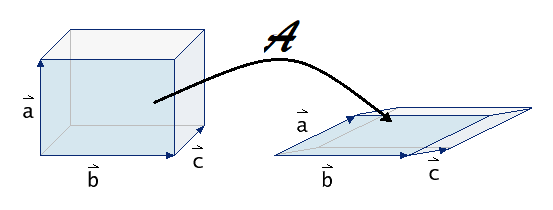
\includegraphics[width=0.6\textwidth]{../Mathematik_1/Bilder/determinante_volumenverlust_dimension.png}
% \end{center}
% \end{defbox}
% 
% F�r einfache geometrische Transformation \(\mathcal A: \mathbb R^2 \to \mathbb R^2, \vec x \to A\vec x\) l��t sich \(\mathrm{det}(A)\) ohne Rechnung angeben:
% \begin{exabox}{Determinanten f�r einfache geometrische Transformationen}{ }
%       \begin{eqnarray*}
% 	\left| \begin{array}{cc} 0 & 0 \\ 0 & 0 \end{array}\right| &=& 0\,, \quad \textnormal{Nullmatrix}\,,\\
% 	\left| \begin{array}{cc} 1 & 0 \\ 0 & 1 \end{array}\right| &=& 1\,, \quad \textnormal{Identische Abbildung}\,,\\
% 	\left| \begin{array}{cc} 2 & 0 \\ 0 & 2 \end{array}\right| &=& 4\,,\quad  \textnormal{Skalierung in zwei Richtungen}\,,\\
% 	\left| \begin{array}{cc} 2 & 0 \\ 0 & 1 \end{array}\right| &=& 2\,,\quad \textnormal{Skalierung in eine Richtung}\,,\\
% 	\left| \begin{array}{cc} \frac{1}{\sqrt{2}} &  -\frac{1}{\sqrt{2}} \\ \frac{1}{\sqrt{2}} &  \frac{1}{\sqrt{2}} \end{array}\right| &=& 1\,,\quad \textnormal{Drehung}\,,\\
% 	\left| \begin{array}{cc} 0 &  1 \\ 1 &  0 \end{array}\right| &=& -1\,,\quad \textnormal{Spigelung, i.e. Vertauschung zweier Spalten}\,,\\
% 	\left| \begin{array}{cc} 1 &  1 \\ 0 &  1 \end{array}\right| &=& 1\,,\quad \textnormal{Scherung in eine Achsenrichtung}\,.
%       \end{eqnarray*}
% \end{exabox}
% 
% Die Determinante zweier Matrizen $A$ und $B$, die man hintereinander anwendet ist  
% \begin{theorembox}{Determinante vom Produkt}{ }
%   $\det(AB)= \det(A)\cdot \det(B)\,.$
% \end{theorembox}
% 
% Hieraus folgen Rechenregeln, die f�r die Determinante bei Spalten- oder Zeilenumformungen gelten m�ssen: 
% \begin{exabox}{Rechenregeln}{ }
%   \begin{enumerate}
%     \item Multiplikation einer Spalte (Zeile) einer Matrix mit einer Zahl:
%       \begin{eqnarray*}
%       \left| \begin{array}{ccc} 2 & -7 & \textcolor{blue}{3} \\ 0 & 2 & \textcolor{blue}{6}  \\ 4 & 1 & \textcolor{blue}{9} \end{array}\right| = \left| \begin{array}{ccc} 2 & -7 & \textcolor{blue}{ 1} \\ 0 & 2 & \textcolor{blue}{2}  \\ 4 & 1 & \textcolor{blue}{3} \end{array}\right| \cdot \left| \begin{array}{ccc} 1 & 0 & 0 \\ 0 & 1 & 0  \\ 0 & 0 & \textcolor{blue}{3} \end{array}\right|  = \textcolor{blue}{3}\, \left| \begin{array}{ccc} 2 & -7 & 1 \\ 0 & 2 & 2  \\ 4 & 1 & 3 \end{array}\right| \,.
%       \end{eqnarray*}
%     \item Vertauschen zweier Spalten (Zeilen) einer Matrix:
%       \begin{eqnarray*}
% 	      \left| \begin{array}{ccc} 2 & \textcolor{blue}{-7} & \textcolor{brown}{3} \\ 0 & \textcolor{blue}{2} & \textcolor{brown}{6}  \\ 4 & \textcolor{blue}{1} & \textcolor{brown}{9} \end{array}\right| = \left| \begin{array}{ccc} 2 & \textcolor{brown}{3} & \textcolor{blue}{-7}  \\ 0 & \textcolor{brown}{6} & \textcolor{blue}{2}  \\ 4 & \textcolor{brown}{9} & \textcolor{blue}{1}  \end{array}\right| \cdot \left| \begin{array}{ccc} 1 & 0 & 0  \\ 0 & 0 & \textcolor{brown}{1}  \\ 0 & \textcolor{blue}{1} & 0  \end{array}\right| = -\left| \begin{array}{ccc} 2 & \textcolor{brown}{3} & \textcolor{blue}{-7}  \\ 0 & \textcolor{brown}{6} & \textcolor{blue}{2}  \\ 4 & \textcolor{brown}{9} & \textcolor{blue}{1}  \end{array}\right| \,.
%       \end{eqnarray*}
% \item Zwei identische Spalten (Zeilen):
%       \begin{eqnarray*}
% 	      \alpha =\left| \begin{array}{ccc} \textcolor{blue}{2} & -7 & \textcolor{brown}{2} \\ \textcolor{blue}{0} & 2 & \textcolor{brown}{0} \\ \textcolor{blue}{4} & 1 & \textcolor{brown}{4} \end{array}\right| \stackrel{2.}{=} - \left| \begin{array}{ccc} \textcolor{brown}{2} & -7 & \textcolor{blue}{2} \\ \textcolor{brown}{0} & 2 & \textcolor{blue}{0} \\ \textcolor{brown}{4} & 1 & \textcolor{blue}{4} \end{array}\right| = - \alpha  \; \Leftrightarrow \; \alpha = 0 \,.
%       \end{eqnarray*}
% \item Eine Spalte (Zeile) einer Matrix als Summer zweier Vektoren:
%       \begin{eqnarray*}
% 	      \left| \begin{array}{cc} 2 & 2 \\ 3 & 5  \end{array}\right| = 
% 	      \left| \begin{array}{cc} \textcolor{blue}{2+}0 & 2 \\ \textcolor{blue}{1+}2 & 5  \end{array}\right| =
% 	      \left| \begin{array}{cc} \textcolor{blue}{2} & 2 \\ \textcolor{blue}{1} & 5  \end{array}\right|  \textcolor{blue}{+}
% 	      \left| \begin{array}{cc} 0 & 2 \\ 2 & 5  \end{array}\right| \,.
%       \end{eqnarray*}
% %\item Addition eines Vielfachen einer Spalte (Zeile) auf eine andere Spalte (Zeile) der Matrix:
% %      \begin{eqnarray*}
% %	      \mathrm{det}\left( \begin{array}{ccc} 2 & -7 & 3 - 2\cdot 7 \\ 0 & 2 & 6+2\cdot2  \\ 4 & 1 & 9+2\cdot 1 \end{array}\right) &=& 
% %	      \mathrm{det}\left( \begin{array}{ccc} 2 & -7 & 3 \\ 0 & 2 & 6  \\ 4 & 1 & 9 \end{array}\right) + \underbrace{2 \mathrm{det}\left( \begin{array}{ccc} 2 & -7 & -7 \\ 0 & 2 & 2  \\ 4 & 1 & 1 \end{array}\right)}_{\displaystyle{= 0}} = 
% %	      \mathrm{det}\left( \begin{array}{ccc} 2 & -7 & 3 \\ 0 & 2 & 6  \\ 4 & 1 & 9 \end{array}\right) \,.
% %      \end{eqnarray*}
% \end{enumerate}
% \end{exabox}
% \noindent\textbf{Bemerkungen:}
% \begin{itemize}
% 	\item Es gilt \(\mathrm{det}(A) = \mathrm{det}(A^\intercal)\) und deshalb gelten die Regeln genauso f�r die entsprechenden Zeilenumformungen.
% 	\item Besitzt eine Abbildung genau diese Eigenschaften dann nennt man sie "\,antisymmetrischen Multilinearform". Die Determinante ist also eine antisymmetrische Multilinearform.
% \end{itemize}
% 
% Mit den Rechenregeln kann man nun die Determinante jeder Matrix berechnen. Wir beginnen mit der Determinante einer $2\times2$-Matrix:
%   \begin{eqnarray*}
% 	  \left| \begin{array}{cc} \textcolor{blue}{1} & \textcolor{brown}{2} \\ \textcolor{brown}{3} & \textcolor{blue}{4}  \end{array}\right| &\stackrel{4.}{=}& \left| \begin{array}{cc} 1 & 2+0 \\0 & 0+4  \end{array}\right| +  \left| \begin{array}{cc} 0 & 2+0 \\3 & 0+4  \end{array}\right| \\[1ex] 
% 	  &\stackrel{1.}{=}& 2\cdot \underbrace{\left| \begin{array}{cc} 1 & 1 \\0 & 0  \end{array}\right|}_{=0 \; (3.)}
%     +  4\cdot \underbrace{\left| \begin{array}{cc} 1 & 0 \\0 & 1  \end{array}\right|}_{=1}  
%     +  2\cdot 3 \underbrace{\left| \begin{array}{cc} 0 & 1 \\1 & 0  \end{array}\right|}_{=-1 \;(1.)} 
%     +  3\cdot 4 \underbrace{\left| \begin{array}{cc} 0 & 0 \\1 & 1  \end{array}\right|}_{=0 \; (3.)}\\[1ex] 
%     &=& \textcolor{blue}{1}\cdot \textcolor{blue}{4} - \textcolor{brown}{2}\cdot \textcolor{brown}{3} = -2 \,.
%   \end{eqnarray*}
% Diese Umformungen sind immer m�glich und deshalb gilt allgemein f�r eine $2\times 2$-Determinante:
% \begin{defbox}{Determinante einer $2\times2$ Matrix}{ }
%   $
%   \left| \begin{array}{cc} \textcolor{blue}{a} & \textcolor{brown}{b} \\ \textcolor{brown}{c} & \textcolor{blue}{d}  \end{array}\right|  = \textcolor{blue}{a}\cdot \textcolor{blue}{d} - \textcolor{brown}{b} \cdot \textcolor{brown}{c}\,.
%     $
% \end{defbox}
% 
% Um die Determinante einer $3\times3$-Matrix zu berechnen, zerlegen wir sie in drei $2\times 2$-"\,Unterdeterminanten":
% \begin{exabox}{Entwicklung nach der ersten Spalte}{ }
%   \begin{eqnarray*}
%     \left| \begin{array}{ccc} \textcolor{blue}{1} & 2 & 3 \\\textcolor{blue}{4} & 5 & 6 \\ \textcolor{blue}{7} & 8 & 9  \end{array}\right| 
%       &=& 
%       \left| \begin{array}{ccc} \textcolor{blue}{1} & 2 & 3 \\0 & 5 & 6 \\0 & 8 & 9  \end{array}\right| 
%       + \left| \begin{array}{ccc} 0 & 2 & 3 \\\textcolor{blue}{4} & 5 & 6 \\0 & 8 & 9  \end{array}\right| 
%       + \left| \begin{array}{ccc} 0 & 3 & 3 \\0 & 5 & 6 \\\textcolor{blue}{7} & 8 & 9  \end{array}\right| \\
%       &=& 
%       \textcolor{blue}{1} \cdot \underbrace{\left| \begin{array}{ccc} \textcolor{brown}{1} & 0 & 0 \\0 & 5 & 6 \\0 & 8 & 9  \end{array}\right|}_{\displaystyle{= \textcolor{brown}{1} \cdot \left| \begin{array}{cc} 5 & 6 \\8 & 9  \end{array}\right|} } 
%       +\; \textcolor{blue}{4} \cdot \underbrace{\left| \begin{array}{ccc} 0 & 2 & 3 \\\textcolor{brown}{1} & 0 & 0 \\0 & 8 & 9  \end{array}\right|}_{\displaystyle{ =\textcolor{brown}{- 1}\cdot \left| \begin{array}{cc} 2 & 3 \\8 & 9  \end{array}\right|} }
%       +\; \textcolor{blue}{7} \cdot \underbrace{ \left| \begin{array}{ccc} 0 & 3 & 3 \\0 & 5 & 6 \\\textcolor{brown}{1} & 0 & 0  \end{array}\right| }_{\displaystyle{= \textcolor{brown}{1}\cdot \left| \begin{array}{cc} 3 & 3 \\5 & 6  \end{array}\right|} }\\
%       &=& \textcolor{brown}{1}\cdot \textcolor{blue}{1}\cdot \left| \begin{array}{cc} 5 & 6 \\8 & 9  \end{array}\right| \textcolor{brown}{- 1 }\cdot \textcolor{blue}{4}\cdot \left| \begin{array}{cc} 2 & 3 \\8 & 9  \end{array}\right|+ \textcolor{brown}{1} \cdot\textcolor{blue}{7} \cdot \left| \begin{array}{cc} 3 & 3 \\5 & 6 \end{array}\right| \\
%       &=& (5\cdot 9 - 6\cdot 8)  - 4  \cdot (2\cdot 9 - 8\cdot 3) + 7 \cdot ( 3\cdot 6 - 5\cdot 3) \\ &=& (45-48)-4\cdot (18-24)+7\cdot (18-15) = -3+24 -21 = 0   \,.
%   \end{eqnarray*}
% \end{exabox}
% 
% Diese Vorgehensweise hei�t "\,Entwicklung nach der ersten Spalte". Entsprechend kann man nach jeder anderen Spalten entwickeln, man muss beim Entwickeln nach anderen Spalten unter Umst�nden Zeilen vertauschen und das f�hrt zu Vorzeichenwechseln. Merken Sie sich die Vorzeichen einfach im Schachbrettmuster:
% \begin{theorembox}{Vorzeichen im Schachbrettmuster}{ }
%   $
%     \left| \begin{array}{ccc} + & - & + \\- & + & - \\+ & - & +  \end{array}\right|\,.
%     $
% \end{theorembox}
% 
% %  Analysiert man diese Berechnung, dann stellt man fest, dass Spalten und Zeilen gleichberechtigt sind, dass also 
% %  \begin{itemize}
% %    \item f�r die Reihen die entsprechenden Rechengesetze gelten wie f�r die Zeilen und 
% %    \item die Determinante beim Transponieren gleich bleibt: $$\det(A^\intercal)= \det(A)$$ 
% %  \end{itemize}
% 
%   Mit entsprechenden Umformungen kann man Determinanten beliebiger Gr��e berechnen. F�r eine $3\times 3$-Determinante findet man die leicht zu merkende Regel von Sarrus.
%   \begin{eqnarray*}
%     \left| \begin{array}{ccc} 1 & 2 & 3 \\4 & 5 & 6 \\7 & 8 & 9  \end{array}\right| \textcolor{lightgray}{\begin{array}{cc} 1 & 2  \\ 4 & 5  \\7 & 8  \end{array}} = 
%       \textcolor{red}{1\cdot 5\cdot 9 + 2\cdot 6 \cdot 7 + 3\cdot4\cdot8} \textcolor{blue}{- 7\cdot 5\cdot 3 - 8\cdot 6 \cdot 1 - 9\cdot4\cdot2}  \,.
%   \end{eqnarray*}
% Vorsicht,  diese  Regel  gilt nicht f�r  $4\times 4$-oder noch gr��ere Determinanten!  
% 
% Wenn man eine $n\times n$-Determinante naiv durch Entwickeln aufdr�selt, muss man die Summe von $n!$ Produkten mit je $n$ Faktoren berechnen. Der Rechenaufwand und die Rundungsfehler explodieren mit gr��eren $n$, selbst wenn man geschickt rechnet. Man schreibt deshalb die Determinanten gr��erer Matrizen allenfalls als Zwischenschritt hin, um Formeln zu vereinfachen, vermeidet aber strikt, solche Determinanten tats�chlich auszurechnen.
% 
% %\subsection{Produkte mit Vektoren}
% 
% Mit der Determinante haben wir alle Hilfsmittel zur Hand, um ein letztes Produkten von Vektoren einzuf�hren: das sogenannte Spatprodukt [triple product] ist eine Sonderausstattung des $\mathbb R^3$ und bildet drei Vektoren auf eine Zahl ab. Es sei $(\vec x_1, \vec x_2, \vec x_3) \in \mathbb R^{3\times 3}$ die Matrix mit den Spaltenvektoren $\vec x_1, \vec x_2$ und $\vec x_3$, dann lautet das Spatprodukt:
% \begin{defbox}{Spatprodukt}{ }
%   $ \mathbb R^3\times \mathbb R^3\times \mathbb R^3 \to \mathbb R, \; \left( \vec x_1, \vec x_2, \vec x_3\right) \mapsto |\vec x_1, \vec x_2, \vec x_3| \,,$ 
% \end{defbox}
% oder, beispielhaft, mit gegebenen Vektoren: 
% \begin{exabox}{Spatprodukt}{ }
%   \begin{eqnarray*}
%     \left( \left( \begin{array}{r} 1 \\ 2 \\ 3\end{array}\right), 
%     \left( \begin{array}{r} 3 \\ 0 \\ 2\end{array}\right), 
%   \left( \begin{array}{r} 4 \\ -2 \\ 1\end{array}\right) \right)
%   \mapsto \left| \begin{array}{ccc} 1 & 3 & 4 \\2 & 0 & -2 \\3 & 2 & 1  \end{array} \right| = -3 \cdot (2\cdot 1 + 3 \cdot 2 ) - 2 \cdot ( - 2\cdot 1 - 2 \cdot 4)  = -4\,. 
%   \end{eqnarray*}
% \end{exabox}
% Das Spatprodukt liefert das Volumen  des Spats, der von den drei Vektoren aufgespannt wird, mit Vorzeichen f�r die Orientierung. 
% 
% %Um das zu verstehen, macht man sich bewu�t, dass die Anwendung einer Matrix, beispielsweise
% %$$
% %    A = \left( \begin{array}{ccc} 1 & 3 & 4 \\2 & 0 & -2 \\3 & 2 & 1  \end{array}\right) \,,
% %$$
% %aus dem Einheitsw�rfel $E$ ein Parallelipiped $P$ macht
% %$$
% %A: E \mapsto AE =: P\,.
% %$$
% %Die Determinante der Matrix $A$ misst wie sich das Volumens des Einheitsw�rfels durch die lineare Transformation ver�ndert. Also  ist  das  Volumen  des  Parallelipeds  mit  Vorzeichen  gleich  der Determinante und damit gleich dem Spatprodukt.
% %\begin{theorembox}{Spatprodukt liefert das Volumem des Spats}{ }
% %  $
% %  \det(A)\underbrace{\mathrm{vol}(E)}_{\displaystyle{=1}} = \mathrm{vol}(P)\; \Rightarrow\; \mathrm{vol}(P) = \det(A)\,. 
% %    $
% %\end{theorembox}
% 
% 
% \subsection{Inverse Matrix}
% 
% Betrachten wir ein lineares Gleichungsystem $A\vec x= \vec b$ mit $n$ Gleichungen und $n$ (also genau so vielen!) Unbekannten. Dann ist die Koeffizientenmatrix $A$ quadratisch und man kann ihre Determinante $\det(A)$ bilden. Die L�sbarkeit des Gleichungssystems kann mit Hilfe der Determinante analysiert werden: 
% \begin{theorembox}{L�sbarkeit von Gleichungssystemen mit \(A\in\mathbb R^{n\times n}\)}{ }
% 	Einer der beiden F�lle tritt ein:
% \begin{itemize}
% 	\item Die Determinante der Koeffizientenmatrix ist null. Dann besitzt das Gleichungssystem nicht f�r alle rechte Seiten eine L�sung. Wenn das Gleichungssystem f�r eine bestimmte rechte Seite l�sbar ist, dann ist die L�sung nicht eindeutig wie im Beispiel $3$ des vorigen Kapitels. 
%     \begin{eqnarray*} 
%       \det(A)=0 &\Leftrightarrow&  \textnormal{mindestens eine Dimension fehlt im Ergebnis} \\
% 	&\Leftrightarrow& \textnormal{rk}(A) < n  \\
% 	& \Leftrightarrow&  \textnormal{def}(A) \geq 1 
%       \end{eqnarray*}
% \item Die Determinante der Koeffizientenmatrix ist nicht null. Dann gibt es f�r das entsprechende Gleichungssystem f�r jede rechte Seite eine eindeutige L�sung wie im Beispiel $4$ des vorigen Kapitels.  
%     \begin{eqnarray*} 
%       \det(A)\not=0 &\Leftrightarrow&  \textnormal{Gleichungssystem eindeutig l�sbar} \\
% 	&\Leftrightarrow& \textnormal{rk}(A) = n  \\
% 	& \Leftrightarrow&  \textnormal{def}(A) = 0\,. 
%       \end{eqnarray*}
% \end{itemize}
% \end{theorembox}
%   
% Im Fall $\det(A) \not = 0$ ist die Abbildung \(\mathcal A: \mathbb R^n \to \mathbb R^n\) also bijektiv: man kann von einem \(\vec x\) immer auf \(\vec b\) und zur�ck schlie�en! Die lineare Abbildung muss also umkehrbar sein un die \underline{Umkehrabbildung}\randverweis{MA1-eigenschaften-von-funktionen} \(\mathcal A^{-1}\) muss wieder linear sein. Die Matrix, die \(\mathcal A^{-1}\) zugeordnet ist, ist die zu $A$ inverse Matrix $A^{-1}$.
% \begin{theorembox}{Existenz der inversen Matrix}{ }
% \[ 
% A\in \mathbb R^{n\times n}, \; \det(A)\not=0 \Rightarrow \; \exists!\; A^{-1}:\mathbb R^n\to\mathbb R^n, \vec b \mapsto \vec x\,.
% \]
% \end{theorembox}
% 
% \noindent\textbf{Bemerkungen:}
% \begin{itemize}
% 	\item Nur quadratische Matrizen $A\in\mathbb R^{n\times n}$ sind invertierbar und das nur, wenn $\det(A)\not=0$.
% 	\item Existiert die inverse Matrix, dann kann man das Gleichungssystem $A\vec x = \vec b$ f�r beliebige rechte Seiten $\vec b \in \mathbb R^n$ l�sen und es gilt \(\vec x = A^{-1} \vec b\).
% 	\item Die Schreibweise $A^{-1}$ ist wie der Kehrwert und wie die Potenz $-1$ bei Zahlen gemeint: Analog zu $3^{-1} \cdot 3= 3 \cdot 3^{-1} = 1$, gilt 
% $$ 
% A^{-1} A=  A A^{-1}= \vec 1\,. \quad \quad (*)
% $$ 
% Bei Zahlen kann man von der Null keinen Kehrwert bilden und entsprechend kann man von nicht quadratischen Matrizen und von Matrizen mit Determinante null keine inverse Matrix bilden. %In MATLAB sowie in Wolfram Alpha schreibt man \verb-inv(A)- oder die Potenz $-1$ f�r die inverse Matrix.
% \end{itemize}
% 
% Die Berechnung der inversen Matrix gelingt wieder durch die Anwendung des \underline{Gau�schen Verfahrens}\randverweis{MA1-matrizen}. Betrachten wir eine regul�re Matrix $A\in\mathbb R^{n\times n}$, dann erh�lt man durch die L�sung des Gleichungssystems
% \[ A \vec x_i = \vec e_i\,, \quad \quad (**) \] 
% gerade die $i$-te Spalte der inversen Matrix $A^{-1}$ - denken Sie an $(*)$. Das hei�t aber, dass man die Gleichungen $(**)$ f�r $i=1,\cdots, n$ simulatan gel�st hat, wenn man die Matrix $A$ in der erweiterten Matrix $(A\,|\, \vec 1)$ mittels �quivalenter Zeilenumformungen (�ZU) in die Einheitsmatrix $\vec 1$ transformiert hat. Die rechte Seite des erweiterten Systems ist dann gerade die inverse Matrix $A^{-1}$:
% \[  \left( A\, | \, \vec 1\right) \stackrel{\textnormal{\"AZU}}{\Rightarrow} \left( \vec 1 \, |\,  B\right) \; \Rightarrow B = A^{-1} \,.\]
% Anders als beim L�sen eines Gleichungssystems, h�ren wir nicht bei der Dreiecksgestalt der Matrix $A$ auf, sondern fahren mit dem Gau�schen Eliminationsverfahren fort und eliminieren auch die Elemente oberhalb der Diagonale. Das entspricht dem Schritt des R�ckw�rts-L�sens im Gau�schen Verfahren. Zuletzt werden die Diagonalelemente auf eins normiert.   
% 
% \begin{exabox}{Berechnung der inversen Matrix $\left(A\, | \, \vec 1 \right) \to \left(\vec 1 \, | \, A^{-1}\right)$}{ }
% 	Betrachten wir beispielsweise die Matrix \[ A=\left( \begin{array}{ccc} 1 & 1 & -1 \\ 2 & 3 & 0 \\ 1 & 0 & 3 \end{array}\right), \quad \mathrm{det}(A) = 6 \not= 0\,. \] Die Determinante von $A$ verschwindet nicht und wir k�nnen die Inverse berechnen: 
% 	\begin{eqnarray*} 
% 		& \left( \begin{array}{ccc | ccc} 1 & 1 & -1 & 1 & 0 & 0  \\ 2 & 3 & 0 & 0 & 1 & 0 \\ 1 & 0 & 3 & 0 & 0 & 1\end{array}\right) \Leftrightarrow
% 		\left( \begin{array}{ccc | ccc} 1 & 1 & -1 & 1& 0 & 0  \\ 0 & 1 & 2 & -2 & 1 & 0 \\ 0 & -1 & 4 & -1 & 0 & 1\end{array}\right) \Leftrightarrow 
% 		\left( \begin{array}{ccc | ccc} 1 & 1 & -1 & 1& 0 & 0  \\ 0 & 1 & 2 & -2 & 1 & 0 \\ 0 & 0 & 6 & -3 & 1 & 1\end{array}\right) \\
% 		\Leftrightarrow  &\left( \begin{array}{ccc | ccc} 1 & 1 & -1 & 1 & 0 & 0  \\ 0 & 1 & 2 & -2 & 1 & 0 \\ 0 & 0 & 6 & -3 & 1 & 1\end{array}\right) \Leftrightarrow 
% 		\left( \begin{array}{ccc | ccc} 6 & 6 & 0 & 3 & 1 & 1  \\ 0 & -3 & 0 & 3 & -2 & 1 \\ 0 & 0 & 6 & -3 & 1 & 1\end{array}\right) \Leftrightarrow 
% 		\left( \begin{array}{ccc | ccc} 6 & 0 & 0 & 9 & -3 & 3  \\ 0 & -3 & 0 & 3 & -2 & 1 \\ 0 & 0 & 6 & -3 & 1 & 1\end{array}\right)  
% 	\end{eqnarray*}
% 	Damit 
% 	\[
% 		A^{-1} = \left( \begin{array}{ccc} \frac32 & -\frac12 & \frac12 \\-1 & \frac23 & - \frac13 \\ -\frac12 & \frac16 & \frac16 \end{array}\right)  \,.
% 	\]
% \end{exabox}
% 
% \subsection{Cramersche Regel (+)}
% 
% Gegeben sei ein lineares Gleichungssystem $A\vec x = \vec b$ mit genauso vielen Gleichungen wie Unbekannten beispielsweise $A \in \mathbb R^{3\times 3}$:
% \[ 
% 	\left( \begin{array}{ccccc} 
% 			82 & 45 & 9 & | & 1 \\ 
% 			27 & 16 & 3 & | & 1 \\ 
% 			 9 & 5  & 1 & | & 0 
% 	\end{array}\right)
% \]
% oder in Vektoren geschrieben:
% \[ 
% 	x_1 \left( \begin{array}{c} 
% 			82  \\ 27  \\ 9  
% 	\end{array}\right) + x_2 
% 	\left( \begin{array}{c} 
% 			45 \\ 16 \\ 5 
% 	\end{array}\right) + x_3 
% 	\left( \begin{array}{c} 
% 			 9 \\ 3 \\ 1 
% 	\end{array}\right) =   
% 	\left( \textcolor{blue}{\begin{array}{c} 
% 			1 \\ 1 \\ 0 
% \end{array}}\right) \quad (*) 
% \]
% 
% Ein mathematisches Experiment: In der Determinante der Koeffizientenmatrix wird die erste Spalte durch die Inhomogenit�t
% ersetzt. Was passiert?
% \begin{eqnarray*} 
% 	\mathrm{det} \left( \begin{array}{ccc} 
% 			\textcolor{blue}{1} & 45 & 9 \\ 
% 			\textcolor{blue}{1} & 16 & 3 \\ 
% 			\textcolor{blue}{0} & 5 & 1   
% 	\end{array}\right)  &\stackrel{(*)}{=}& \mathrm{det} \left( 
% 	x_1 \left( \begin{array}{c} 
% 			82  \\ 27  \\ 9  
% 	\end{array}\right) + x_2 
% 	\left( \begin{array}{c} 
% 			45 \\ 16 \\ 5 
% 	\end{array}\right) + x_3 
% 	\left( \begin{array}{c} 
% 			 9 \\ 3 \\ 1 
% 	\end{array}\right)     \begin{array}{cc}
% 			 45 & 9 \\ 
% 			 16 & 3 \\ 
% 			 5 & 1   
% 	 \end{array}\right) \\ 
% 	 &=& x_1 \cdot 
% 	\mathrm{det} \left( \begin{array}{ccc} 
% 			82 & 45 & 9 \\ 
% 			27 & 16 & 3 \\ 
% 			9 & 5 & 1   
% 	\end{array}\right) = x_1 \cdot \mathrm{det}(A)\,. 
% \end{eqnarray*}
% 
% Wenn also die Koeffizientendeterminante nicht null ist $\mathrm{det}(A)\not = 0$, hat man damit $x_1$ eindeutig bestimmt!
% Wir  wissen  schon  von  der  inversen  Matrix,  dass  man  auch  nur  in diesem Fall sicher eine eindeutige L�sung hat. Analog findet man f�r $x_2$ und $x_3$:
% \begin{exabox}{Cramersche Regel zum L�sen eines Gleichungssystems $A \vec x = \vec b$}{ }
% 	\begin{eqnarray*}
% 		x_1 &=& \frac{1}{\mathrm{det}(A)} 
% 		\mathrm{det}\left( \begin{array}{ccc} 
% 			\textcolor{blue}{1} & 45 & 9 \\ 
% 			\textcolor{blue}{1} & 16 & 3 \\ 
% 	\textcolor{blue}{0} & 5  & 1   \end{array}\right)  = 1\,,\\
% 		x_2 &=& \frac{1}{\mathrm{det}(A)} 
% 		\mathrm{det}\left( \begin{array}{ccc} 
% 			82 & \textcolor{blue}{1} & 9 \\ 
% 			27 & \textcolor{blue}{1} & 3 \\ 
% 	9  & \textcolor{blue}{0} & 1   \end{array}\right) = 1 \,,\\ 
% 		x_3 &=& \frac{1}{\mathrm{det}(A)} 
% 		\mathrm{det}\left( \begin{array}{ccc} 
% 			82 & 45 & \textcolor{blue}{1}  \\ 
% 			27 & 16 & \textcolor{blue}{1}  \\ 
% 	9  & 5  & \textcolor{blue}{0}    \end{array}\right) = -14 \,.
% \end{eqnarray*}
% \end{exabox}
% 
% Diese Cramersche Regel [Cramer�s rule] gilt offensichtlich auch f�r zwei Gleichungen mit zwei Unbekannten oder $78$ Gleichungen mit $78$ Unbekannten. Allerdings sollten Sie folgendes beachten:
% \begin{itemize}
% 	\item Die Cramersche Regel ist dann anzuwenden, wenn man nur an einer L�sungskomponente des Gleichungssystems interessiert ist.
%   \item Die Cramersche Regel funktioniert nur, wenn es genauso viele Gleichungen wie Unbekannte gibt (quadratische Gleichungssysteme).
%   \item Die Cramersche Regel funktioniert nur, wenn das Gleichungssystem genau eine L�sung hat, also wenn die Koeffizientenmatrix eine inverse Matrix besitzt, also wenn die Koeffizientendeterminante nicht null ist.
%   \item Wenn die Zahl von Unbekannten und Gleichungen gro� ist, explodieren durch die Berechnung der Determinanten der Rechenaufwand und die Rundungsfehler (numerische Instabilit�t).
% \end{itemize}
% 
% 
 \newpage % Determinante und Inverse
\setcounter{exercise}{0} 
\ifintegriereaufgaben
\section*{Determinante, inverse Matrix Aufgaben}\label{MA1-determinante-und-inverse-aufgaben}

	Regeln und Beispiele, die zur Bearbeitung der Aufgaben hilfreich sind, finden Sie im Skript\wennreferenzvorhanden{MA1-determinante-und-inverse}{ (Abschnitt \abschnittsverweis{MA1-determinante-und-inverse})} und, falls Sie nicht weiterkommen, schauen Sie \hyperref[MA1-determinante-und-inverse-loesungen]{hier}.
\else
\section{Determinante, inverse Matrix Aufgaben}\label{MA1-determinante-und-inverse-aufgaben}

	Regeln und Beispiele, die zur Bearbeitung der Aufgaben hilfreich sind, finden Sie im Skript und, falls Sie nicht weiterkommen, schauen Sie \hyperref[MA1-determinante-und-inverse-loesungen]{hier}.
\fi 

\begin{exercisebox}[Determinante]
	Berechnen Sie die Determinante der Matrix \[ A = \left( \begin{array}{ccc} 2 & -6 & 2 \\ 0 & 0 & 2 \\ -1 & 2 & 1 \end{array}\right)\,.  \]

\end{exercisebox}

\begin{exercisebox}[Determinante]
	Betrachten Sie die Schar der Matrizen \[ A_a = \left( \begin{array}{ccc} 1 & 1 & a \\ 1 & a & 1 \\ 1 & a & a \end{array}\right)\,, \quad a \in \mathbb R\,. \] 
	\begin{itemize}
		\item[(a)] Berechnen Sie die Determinante von $A_a$.
		\item[(b)] F�r welche $a\in \mathbb R$ ist $A_a$ regul�r?
		\item[(c)] Berechnen Sie mit Hilfe des Gau�-Algorithmus die inversen Matrizen $A_a^{-1}$ f�r alle regul�ren Matrizen $A_a$.
		\item[(d)] Berechnen Sie mit Hilfe der Cramerschen Regel die erste Spalte der inversen Matrizen $A_a^{-1}$ f�r alle regul�ren Matrizen $A_a$. Hinweis: L�sen Sie $ A_a \boldsymbol v = \boldsymbol e_1, \quad \boldsymbol e_1 = (1, 0, 0)^\intercal\,.$

\end{itemize}

\end{exercisebox}
\begin{exercisebox}[Basis]
	�berpr�fen Sie mit Hilfe der Determinante, ob die Vektoren 
	\[ 
		\boldsymbol v_1 = ( 2, -1, 0)^\intercal, \quad  
		\boldsymbol v_2 = ( 1, 1, 2 )^\intercal, \quad 
	\boldsymbol v_3 = ( -5, 1,-2 )^\intercal \]
	eine Basis des $\mathbb R^3$ sind.
\end{exercisebox}

\begin{exercisebox}[Gleichungssysteme]
	\begin{itemize}
		\item[(a)] Zeigen Sie, dass die Matrix 
			\[ A = \left( \begin{array}{ccc} 1 & 2 & 0 \\ 1 & 7 & 4 \\ 3 & 13 & 4 \end{array}\right) \]
			regul�r ist. 

		\item[(b)] L�sen Sie das lineare Gleichungssystem f�r $x, y, z \in \mathbb R$
	\[ \begin{array}{ccccccc} 
			x_1 & + & 2x_2 & && = & x \\ 
			x_1 & + & 7x_2 &+ & 4x_3 & = & y \\ 
			3x_1 & + & 13x_2 &+ & 4x_3 & = & z 
	\end{array} \]
		\item[(c)] L�sen Sie das lineare Gleichungssystem f�r $x=3, y=8, z=0$
	\end{itemize}
\end{exercisebox}

\begin{exercisebox}[Anwendungen: Eigenwerte]
	Berechnen Sie alle $\lambda \in \mathbb C$, f�r die die Matrix $A- \lambda I_2$ nicht regul�r ist, wobei \[ A = \left( \begin{array}{cc} -11 & 12 \\ -9 & 10 \end{array}\right)\]. 
\end{exercisebox}

%\begin{itemize}
%	\item Erkl�rung: antisymmetrische Multilinearform
%	\item Spatprodukt, Vektorprodukt, Skalarprodukt
%	\item Kleinste Fehlerquadrate - lineaeres Gleichungssystem
%\end{itemize}

%\subsection{Details und Extras}
%\begin{mybox}[Inverse Matrix]
%  Es seien $A,B \in \mathbb R^{n\times n}$ invertierbar. Es gilt 
%  \begin{itemize}
%    \item $\left( A^{-1}\right)^{-1} = A$
%    \item $\left( A B\right)^{-1} = B^{-1} A^{-1}$
%  \end{itemize}
%\end{mybox}
 \newpage 
\setcounter{satz}{0} \setcounter{def}{0} \setcounter{exa}{0}  \section{Grenzwerte von Folgen und Funktionen}\label{MA1-grenzwerte-von-folgen-und-funktionen}

\begin{table}[H]
  \centering
  \begin{tabularx}{\textwidth}{p{0.9\textwidth} p{0.1\textwidth}}
    \toprule
    \multicolumn{2}{c}{\textbf{�bersicht �ber Lernziele und Voraussetzungen}}\\
    \midrule
    \textbf{Lernziele} & \\[.5\normalbaselineskip]
    \tabitem Folgen als mathematische Beschreibung schrittweiser Prozesse und
    Ann�herungen erkl�ren &\\
    \tabitem Konvergenz und Grenzwert einer Zahlenfolge anschaulich und
    mathematisch interpretieren &\\
    \tabitem Grenzwerte elementarer Zahlenfolgen mithilfe von Grenzwerts�tzen
    bestimmen &\\
    \tabitem den Grenzwert einer Funktion an einer Stelle sowie einseitige
    Grenzwerte erkl�ren und bestimmen &\\
    \tabitem Grenzwerte als Grundlage f�r Stetigkeit und Differenzierbarkeit
    einordnen &\\
    \midrule
    \textbf{Voraussetzungen} & \\[.5\normalbaselineskip]
    \tabitem asymptotisches Verhalten von Standardfunktionen, insbesondere
    von rationalen Funktionen & \abschnittsverweis{MA1-polynome}\\
    \bottomrule
  \end{tabularx}
\end{table}

\ifintegriereaufgaben
\noindent �bungsaufgaben zum Thema:
\hyperref[MA1-grenzwerte-von-folgen-und-funktionen-aufgaben]{Aufgaben}
\vspace{0.3cm}
\hrule
\fi


\subsection{Was ist eine Folge?}

Viele mathematische Prozesse entstehen schrittweise. Eine Gr��e wird
wiederholt berechnet, ver�ndert oder angen�hert, wobei jeder Schritt einen
neuen Wert liefert. Eine geordnete Auflistung solcher mathematischer
Objekte hei�t \textbf{Folge} (\emph{sequence}).

Eine Folge kann beispielsweise aus Zahlen, Vektoren oder auch Funktionen
bestehen. In diesem Abschnitt stehen zun�chst Folgen reeller Zahlen im
Mittelpunkt.

Eine Folge l�sst sich als Funktion auffassen, deren Argument nicht
kontinuierlich variiert, sondern die nat�rlichen Zahlen durchl�uft. Jedem
Index \(n\) wird genau ein Folgenglied \(a_n\) zugeordnet. Ist der
Wertebereich \(\mathbb R\), so hei�t die Folge
\textbf{Zahlenfolge} (\emph{sequence of real numbers}):
\[
(a_n)_{n\in\mathbb N^+}:
\mathbb N^+\to\mathbb R,
\qquad
n\mapsto a_n.
\]

\begin{exabox}{Folgen von Zahlen}{ }
  \begin{tabular}{c|ccccc}
    \(n\)   & \(1\) & \(2\) & \(3\) & \(4\) & \(\dots\)\\
    \hline
    \(a_n\) & \(5\) & \(7\) & \(9\) & \(11\) & \(\dots\)\\
    \(b_n\) & \(1/1\) & \(1/2\) & \(1/3\) & \(1/4\) & \(\dots\)\\
    \(c_n\) & \(3\) & \(3{,}1\) & \(3{,}14\) & \(3{,}141\) & \(\dots\)
  \end{tabular}
\end{exabox}

Die drei Folgen zeigen bereits sehr unterschiedliche Verhaltensweisen.
Die Folgenglieder von \((a_n)_n\) werden immer gr��er. Die Folgenglieder
von \((b_n)_n\) werden dagegen immer kleiner und n�hern sich dem Wert
\(0\). Die Folge \((c_n)_n\) beschreibt eine schrittweise Ann�herung an
die Kreiszahl \(\pi\).

Gerade solche Ann�herungsprozesse spielen in der Analysis eine zentrale
Rolle. Eine Folge erm�glicht es, mathematisch pr�zise zu beschreiben, was
geschieht, wenn ein Prozess immer weiter fortgesetzt wird.


\subsubsection*{Bildungsgesetze}

Da eine unendliche Folge nicht durch die Auflistung aller ihrer
Folgenglieder angegeben werden kann, wird sie typischerweise durch ein
\textbf{Bildungsgesetz} beschrieben.

Bei einer \textbf{explizit definierten Folge} l�sst sich jedes
Folgenglied unmittelbar aus seinem Index berechnen. Bei einer
\textbf{rekursiv definierten Folge} wird ein neues Folgenglied aus bereits
bekannten Folgengliedern bestimmt.

\begin{exabox}{Explizite und rekursive Darstellung einer Folge}{ }

Die Folge
\[
5,\ 7,\ 9,\ 11,\ldots
\]
kann auf zwei verschiedene Arten beschrieben werden.

\medskip
\textbf{Explizite Darstellung:}
Jedes Folgenglied l�sst sich unmittelbar aus dem Index \(n\) bestimmen:
\[
a_n=3+2n,
\qquad n\in\mathbb N^+.
\]

\textbf{Rekursive Darstellung:}
Ausgehend vom ersten Folgenglied wird jedes weitere Folgenglied aus dem
vorhergehenden berechnet:
\[
a_1=5,
\qquad
a_{n+1}=a_n+2.
\]

Beide Bildungsgesetze beschreiben somit dieselbe Folge
\[
(a_n)_n=(5,7,9,11,\ldots).
\]
\end{exabox}


%\noindent\textbf{Ausblick:}
%Viele numerische N�herungsverfahren erzeugen rekursiv definierte Folgen.
%Ein sp�ter verwendetes Beispiel ist das
%\underline{Newton-Verfahren}\randverweis{MA1-lineare-funktionen}
%zur n�herungsweisen Bestimmung von Nullstellen.
%
%\begin{exabox}{Newton-Verfahren}{ }
%Gesucht seien die Nullstellen einer differenzierbaren Funktion \(f\).
%Ausgehend von einem Startwert \(x_0\) erzeugt das Newton-Verfahren eine
%Folge von N�herungswerten durch
%\[
%x_{n+1}
%=
%x_n-\frac{f(x_n)}{f'(x_n)}.
%\]
%Unter geeigneten Voraussetzungen n�hern sich diese Werte einer Nullstelle
%von \(f\). Das Verfahren zeigt damit exemplarisch, weshalb Folgen f�r
%N�herungsprozesse von Bedeutung sind.
%\end{exabox}


\subsection{Grenzwerte von Zahlenfolgen}

Folgen k�nnen sehr unterschiedliche Verhaltensweisen zeigen. Sie k�nnen
wachsen oder fallen, zwischen verschiedenen Werten wechseln, beschr�nkt
bleiben oder unbegrenzt wachsen.

Die folgenden Skizzen veranschaulichen einige dieser M�glichkeiten.

\begin{exabox}{Eigenschaften von Zahlenfolgen}{ }
  \begin{minipage}{0.5\textwidth}
    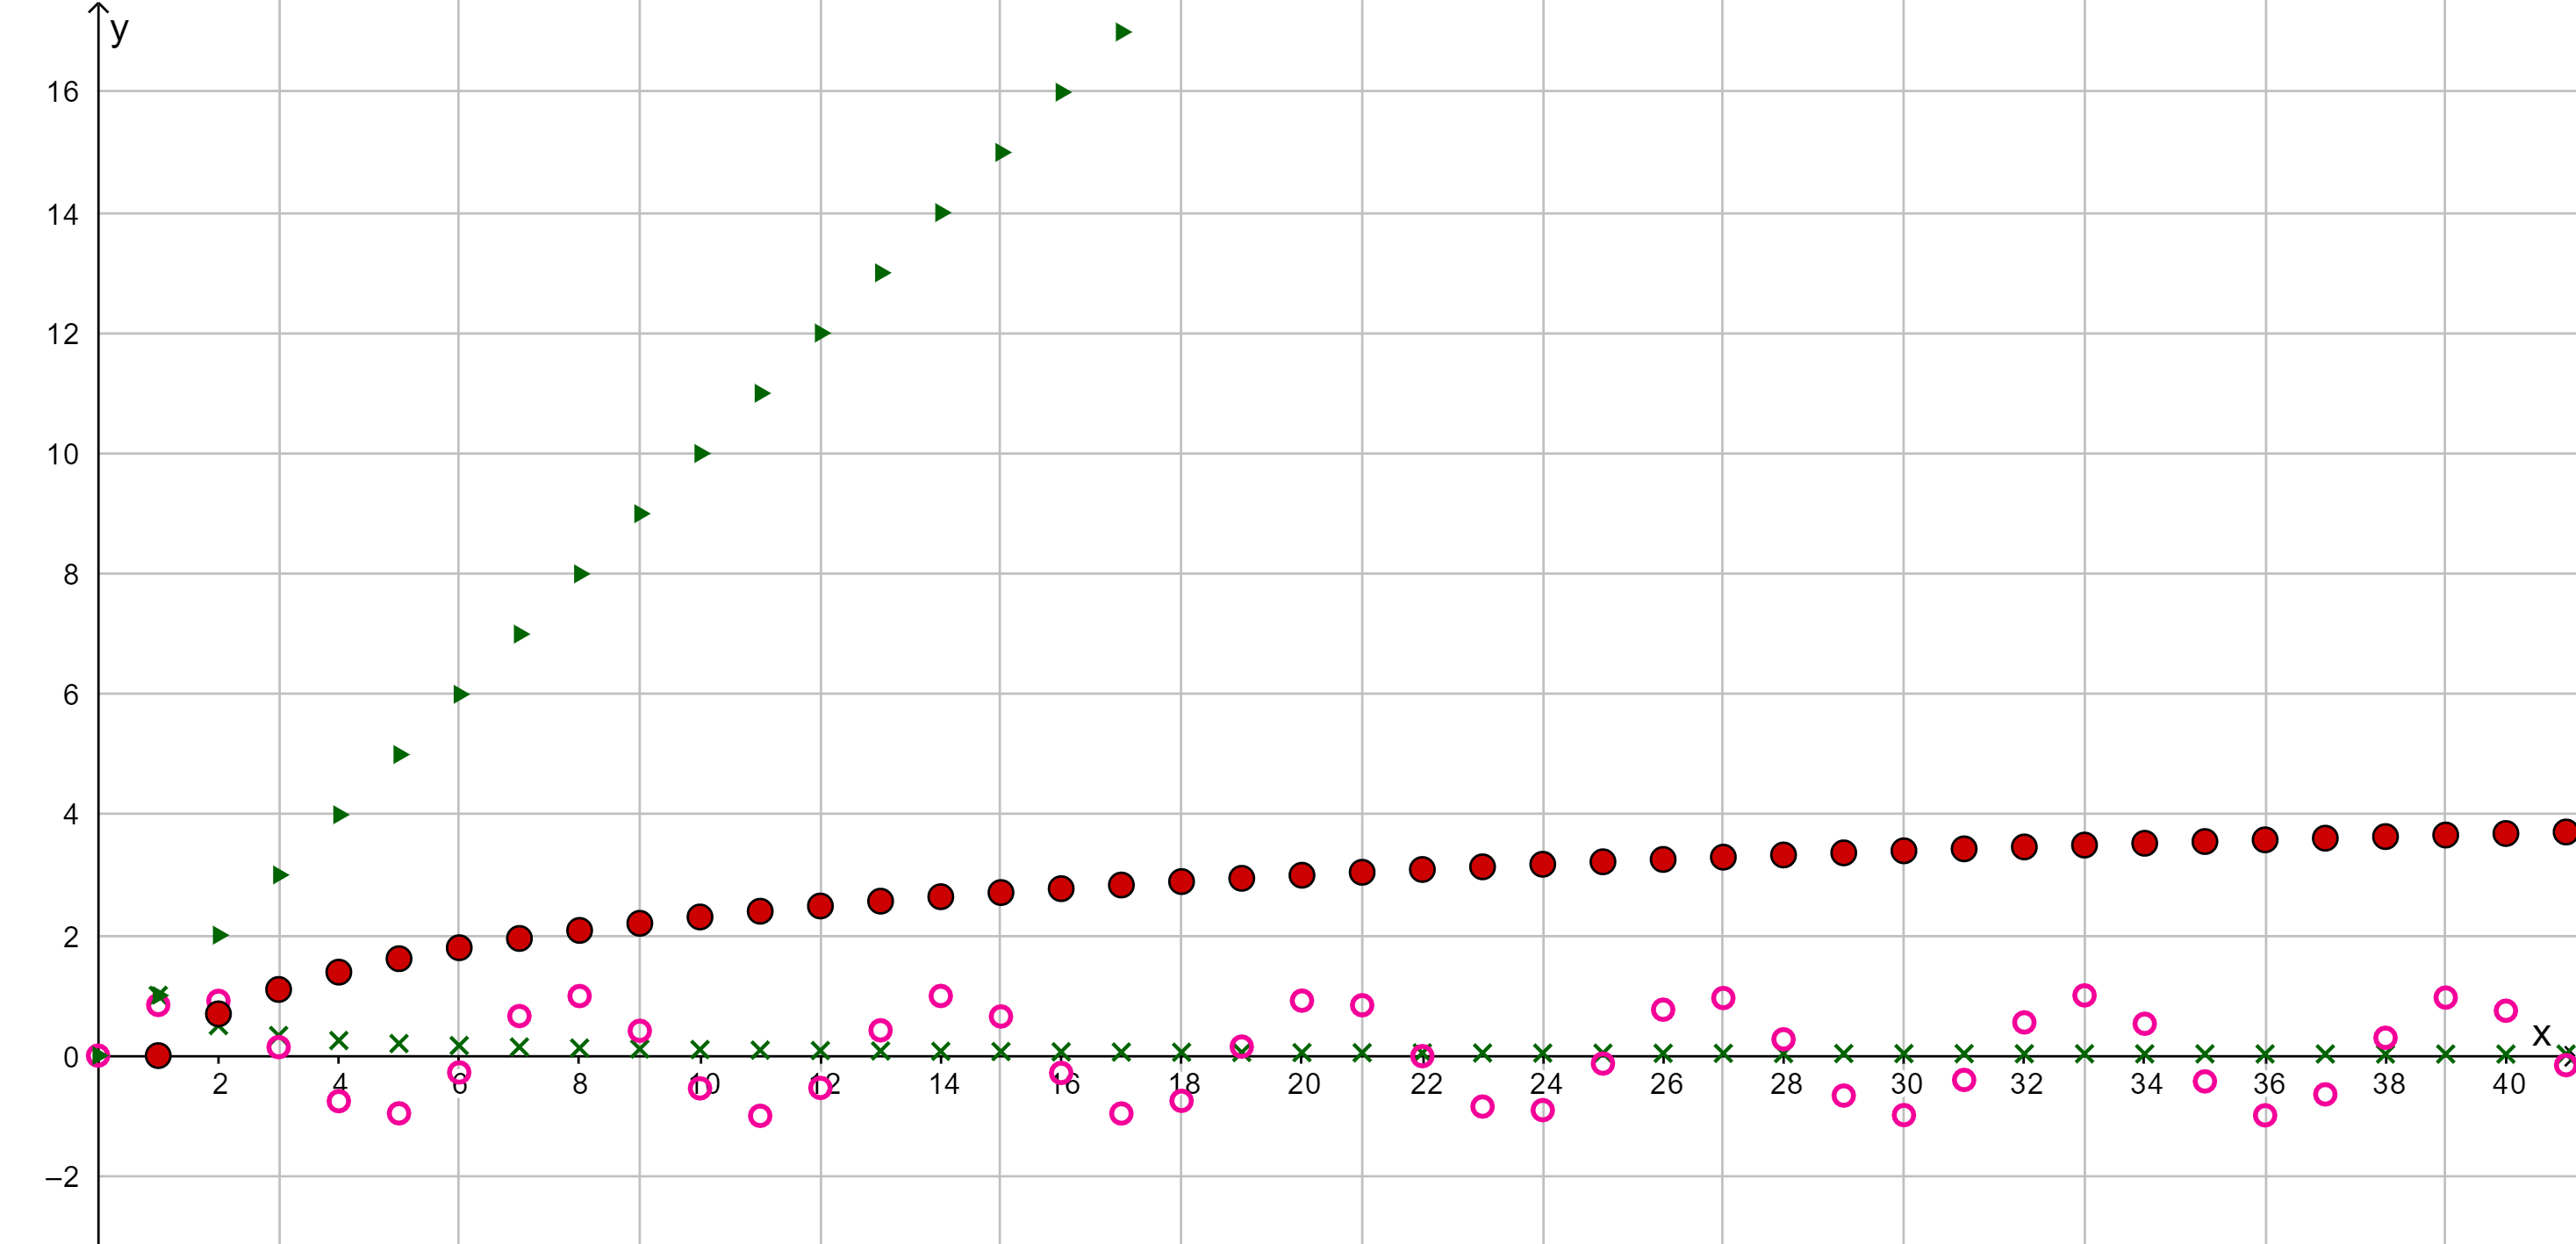
\includegraphics[width=\textwidth]
    {../Mathematik_1/Bilder/folgen_vergleich_eigenschaften.png}
  \end{minipage}
  \begin{minipage}{0.5\textwidth}
    Die dargestellten Folgen unterscheiden sich beispielsweise hinsichtlich
    folgender Eigenschaften:
    \begin{itemize}
      \item beschr�nkt oder unbeschr�nkt,
      \item wachsend oder fallend,
      \item periodisch,
      \item konstant.
    \end{itemize}
  \end{minipage}
\end{exabox}

F�r die folgenden �berlegungen steht eine andere Frage im Mittelpunkt:
\emph{N�hern sich die Folgenglieder f�r zunehmendes \(n\) immer weiter
einem bestimmten Wert an?}

Ein besonders einfaches Beispiel liefert die Folge
\[
a_n=\frac1n.
\]
Ihre ersten Folgenglieder lauten
\[
1,\quad\frac12,\quad\frac13,\quad\frac14,\quad\ldots
\]
und werden immer kleiner. Kein Folgenglied ist gleich \(0\). Trotzdem
lassen sich die Folgenglieder durch hinreichend gro�es \(n\) beliebig nahe
an \(0\) heranbringen.

Dieses Ann�herungsverhalten beschreibt der
\textbf{Grenzwert} (\emph{limit}). F�r das Beispiel gilt
\[
\lim_{n\to\infty}\frac1n=0.
\]

Allgemein bedeutet
\[
\lim_{n\to\infty}a_n=a
\qquad\text{oder kurz}\qquad
a_n\to a,
\]
dass sich die Folgenglieder \(a_n\) f�r zunehmendes \(n\) beliebig nahe
an den Wert \(a\) ann�hern.

Entscheidend ist dabei nicht, ob der Grenzwert \(a\) von der Folge jemals
erreicht wird. Entscheidend ist, dass die Folgenglieder ab einem
hinreichend gro�en Index beliebig nahe bei \(a\) liegen und anschlie�end
auch dort bleiben.


\subsubsection*{Konvergenz}

Die Vorstellung einer Ann�herung l�sst sich mathematisch pr�zisieren.
Dazu wird um den vermuteten Grenzwert \(a\) eine beliebig kleine Umgebung
betrachtet. Ihre Gr��e wird durch eine Zahl \(\varepsilon>0\) beschrieben.

Konvergenz bedeutet, dass sich f�r jede noch so kleine Wahl von
\(\varepsilon\) ein Index finden l�sst, ab dem alle weiteren
Folgenglieder in dieser Umgebung liegen.

\begin{defbox}{Konvergenz einer Zahlenfolge}{ }
Eine Zahlenfolge \((a_n)_n\) hei�t
\textbf{konvergent} (\emph{convergent}) mit Grenzwert \(a\in\mathbb R\),
wenn
\[
\forall\,\varepsilon>0\;
\exists\,N\in\mathbb N^+\;
\forall\,n\geq N:
\qquad
|a_n-a|<\varepsilon.
\]

In diesem Fall gilt
\[
a_n\to a
\qquad\Longleftrightarrow\qquad
\lim_{n\to\infty}a_n=a.
\]

\begin{center}
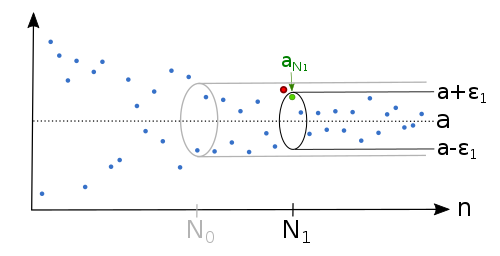
\includegraphics[width=0.55\textwidth]
{../Mathematik_1/Bilder/folgen_konvergenz_epsilon_index.png}
\end{center}
\end{defbox}

Die formale Definition beschreibt genau die zuvor entwickelte
Vorstellung. Die Zahl \(\varepsilon\) gibt einen beliebig kleinen
zul�ssigen Abstand vom Grenzwert \(a\) vor. Zu jedem solchen Abstand
existiert ein Index \(N\). F�r alle \(n\geq N\) gilt dann
\[
|a_n-a|<\varepsilon.
\]
Ab diesem Index liegen also alle weiteren Folgenglieder in der
\(\varepsilon\)-Umgebung des Grenzwerts.

Die Definition dient hier vor allem dazu, die Bedeutung des
Grenzwertbegriffs pr�zise zu erfassen. Grenzwerte werden im Folgenden
nicht durch die direkte Anwendung dieser Definition bestimmt, sondern
mithilfe bekannter Grenzwerte und Grenzwerts�tze.


\begin{exabox}{Ann�herung an einen Grenzwert}{ }
F�r
\[
a_n=\frac{n^2+2}{3n^2}
\]
gilt
\[
a_n
=
\frac{1+\frac{2}{n^2}}{3}.
\]
Da \(2/n^2\) f�r zunehmendes \(n\) gegen \(0\) strebt, n�hern sich die
Folgenglieder dem Wert \(1/3\):
\[
\lim_{n\to\infty}a_n=\frac13.
\]
\end{exabox}


\begin{exabox}{Eine Nullfolge}{ }
F�r die Folge
\[
a_n=\frac3n
\]
gilt
\[
3,\quad\frac32,\quad1,\quad\frac34,\quad\ldots
\longrightarrow0.
\]
Eine Folge mit Grenzwert \(0\) hei�t \textbf{Nullfolge}.
\end{exabox}


\subsubsection*{Konvergenz und Divergenz}

Nicht jede Folge n�hert sich einem festen Wert. Eine Folge, die keinen
endlichen Grenzwert besitzt, hei�t
\textbf{divergent} (\emph{divergent}).

Dabei k�nnen unterschiedliche Formen der Divergenz auftreten. Die Folge
\[
a_n=(-1)^n
\]
wechselt beispielsweise dauerhaft zwischen \(1\) und \(-1\) und n�hert
sich keinem einzelnen Wert.

Eine andere Situation liegt vor, wenn die Folgenglieder schlie�lich �ber
jede vorgegebene Schranke hinauswachsen. In diesem Fall schreibt man
\[
a_n\to\infty.
\]
Entsprechend beschreibt
\[
a_n\to-\infty
\]
eine Folge, deren Werte schlie�lich unter jede vorgegebene Schranke
fallen. Solche Folgen hei�en \textbf{bestimmt divergent}.

\begin{exabox}{Bestimmt divergente Folgen}{ }
\[
n^2\to\infty,
\qquad
e^n\to\infty,
\qquad
\sqrt n\to\infty.
\]
\end{exabox}

Das Symbol \(\infty\) bezeichnet dabei keine reelle Zahl. Eine bestimmt
divergente Folge besitzt daher keinen Grenzwert in \(\mathbb R\).


\noindent\textbf{Bemerkungen:}
\begin{itemize}
  \item Jede konvergente Folge ist beschr�nkt. Die Umkehrung gilt nicht.
  Eine beschr�nkte Folge kann also trotzdem divergent sein.

  \item Monotonie und Beschr�nktheit k�nnen verwendet werden, um
  Konvergenz nachzuweisen. Beispielsweise ist jede nach oben beschr�nkte
  monoton wachsende Folge konvergent. Entsprechend ist jede nach unten
  beschr�nkte monoton fallende Folge konvergent.

  \item Solche Kriterien zum Nachweis von Konvergenz stehen hier nicht im
  Mittelpunkt. Entscheidend ist die Bedeutung des Grenzwerts als
  mathematische Beschreibung eines Ann�herungsprozesses.
\end{itemize}


\begin{exabox}{Beschr�nktheit reicht nicht aus}{ }
  \begin{minipage}{0.5\textwidth}
    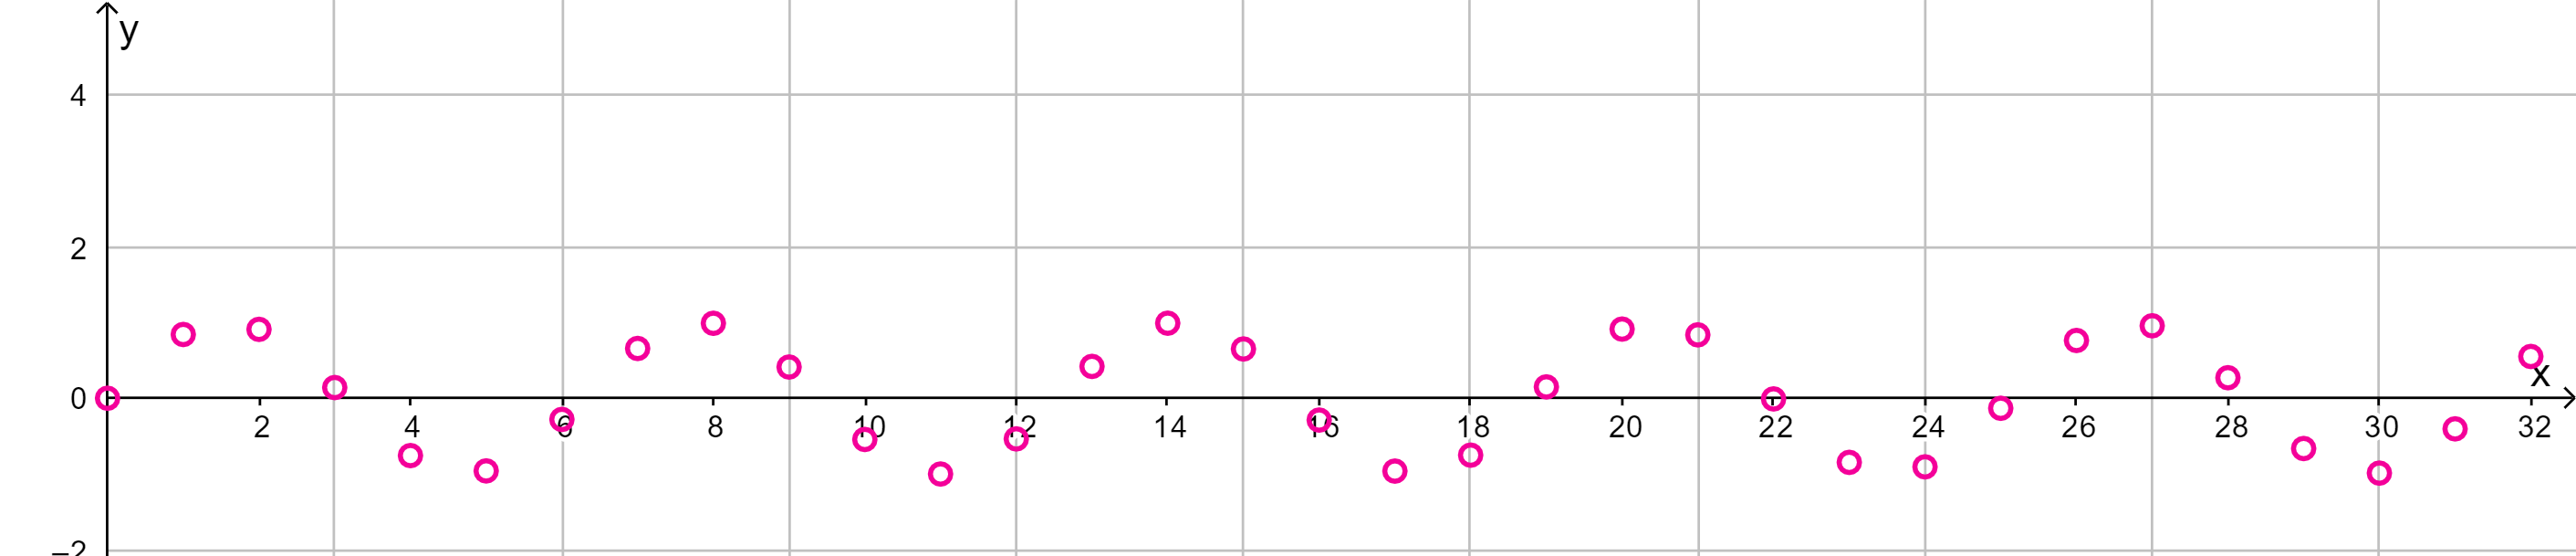
\includegraphics[width=\textwidth]
    {../Mathematik_1/Bilder/folgen_beschraenkt_divergent_oszillation.png}
  \end{minipage}
  \begin{minipage}{0.45\textwidth}
    Eine Folge kann beschr�nkt sein und trotzdem keinen Grenzwert besitzen.
    Beschr�nktheit ist damit notwendig, aber nicht ausreichend f�r
    Konvergenz.
  \end{minipage}
\end{exabox}


\begin{exabox}{Beschr�nktheit und Monotonie}{ }
  \begin{minipage}{0.5\textwidth}
    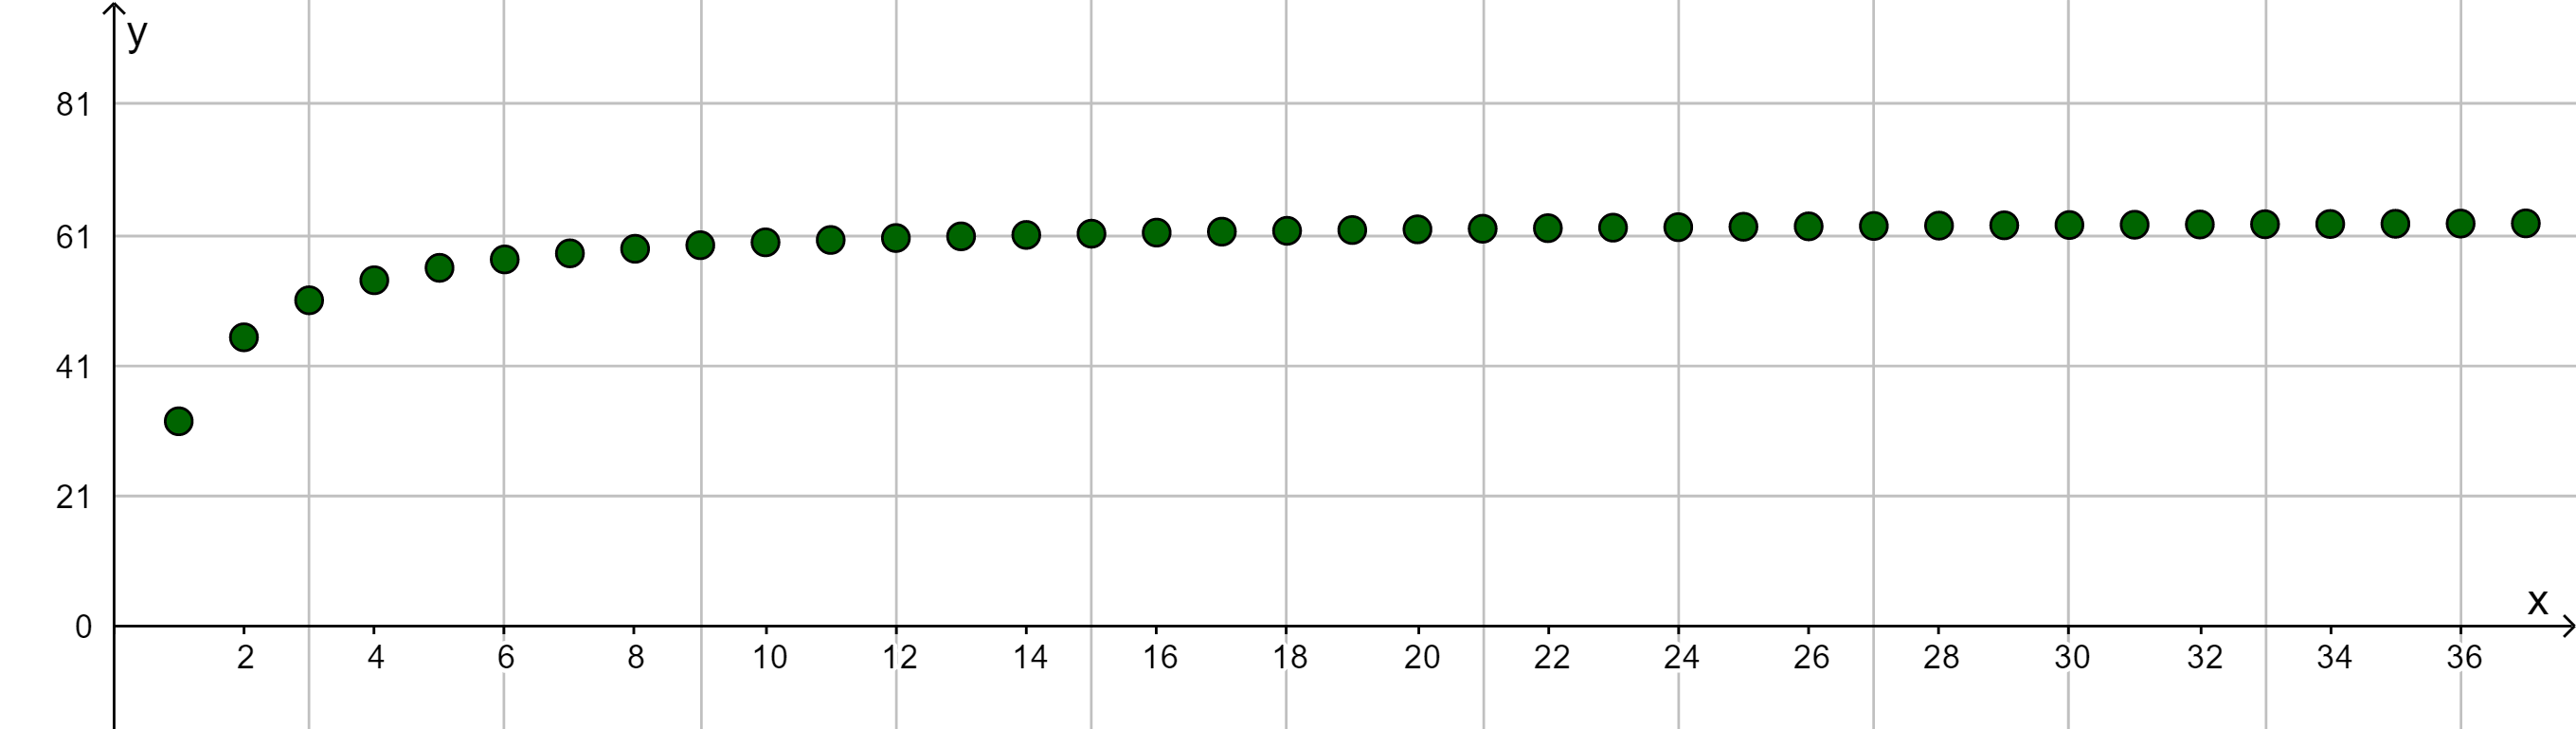
\includegraphics[width=\textwidth]
    {../Mathematik_1/Bilder/folgen_beschraenkt_monoton_konvergent.png}
  \end{minipage}
  \begin{minipage}{0.45\textwidth}
    Eine beschr�nkte monotone Folge ist konvergent. In der dargestellten
    Situation n�hern sich die Folgenglieder einem festen Grenzwert.
  \end{minipage}
\end{exabox}


\subsubsection*{Grenzwerte berechnen}

In praktischen Anwendungen wird ein Grenzwert in der Regel nicht mithilfe
der formalen Definition berechnet. Stattdessen werden bekannte Grenzwerte
und Rechenregeln miteinander kombiniert.

\begin{theorembox}{Grenzwerts�tze f�r Folgen}{ }
Es seien \((a_n)_n\) und \((b_n)_n\) konvergente Zahlenfolgen mit
\[
a_n\to a,
\qquad
b_n\to b.
\]
Dann gilt:
\[
\begin{array}{rcl}
a_n+b_n &\to& a+b,\\[0.5ex]
a_n-b_n &\to& a-b,\\[0.5ex]
a_n\cdot b_n &\to& a\cdot b,\\[0.5ex]
\dfrac{a_n}{b_n} &\to& \dfrac ab
\qquad\textnormal{f�r } b\neq0.
\end{array}
\]

Ist au�erdem \((c_n)_n\) beschr�nkt und gilt
\(|d_n|\to\infty\), so folgt
\[
\frac{c_n}{d_n}\to0.
\]
\end{theorembox}


\begin{exabox}{Ein einfacher Grenzwert}{ }
F�r
\[
a_n=\frac{2n+1}{n}
\]
ergibt sich durch Umformen
\[
\lim_{n\to\infty}\frac{2n+1}{n}
=
\lim_{n\to\infty}\left(2+\frac1n\right)
=
2+0
=
2.
\]
\end{exabox}


\begin{exabox}{Gebrochenrationaler Ausdruck: h�chste Potenz ausklammern}{ }
F�r
\[
\lim_{n\to\infty}
\frac{n^2+\sin(n)}{2n^2+e^{-n}}
\]
wird Z�hler und Nenner durch die h�chste auftretende Potenz \(n^2\)
geteilt:
\[
\lim_{n\to\infty}
\frac{n^2+\sin(n)}{2n^2+e^{-n}}
=
\lim_{n\to\infty}
\frac{1+\frac{\sin(n)}{n^2}}
     {2+\frac{e^{-n}}{n^2}}
=
\frac{1+0}{2+0}
=
\frac12.
\]
Dabei gilt
\[
\left|\frac{\sin(n)}{n^2}\right|
\leq
\frac1{n^2}\to0
\]
und ebenfalls
\[
\frac{e^{-n}}{n^2}\to0.
\]
\end{exabox}


Einige h�ufig auftretende Grenzwerte werden im Folgenden als Referenz
zusammengestellt. Ihre Herleitung steht hier nicht im Mittelpunkt.

\begin{theorembox}{Wichtige Grenzwerte von Folgen}{ }
\begin{itemize}
  \item
  \(\displaystyle
  \lim_{n\to\infty}\left(1+\frac1n\right)^n=e.
  \)

  \item F�r \(a>0\):
  \[
  n^a\to\infty,
  \qquad
  \frac1{n^a}\to0.
  \]

  \item F�r \(|q|<1\) und \(a\in\mathbb R\):
  \[
  q^n\to0,
  \qquad
  n^a q^n\to0.
  \]

  \item F�r \(q>1\) und \(a\in\mathbb R\):
  \[
  q^n\to\infty,
  \qquad
  \frac{q^n}{n^a}\to\infty.
  \]
\end{itemize}
\end{theorembox}


\subsection{Grenzwerte von Funktionen}

Der Grenzwertbegriff f�r Folgen beschreibt einen Ann�herungsprozess:
W�hrend der Index \(n\) immer gr��er wird, k�nnen sich die Folgenglieder
\(a_n\) einem bestimmten Wert ann�hern.

Dieselbe Grundidee l�sst sich auf Funktionen �bertragen. Nun n�hert sich
nicht der Index \(n\) dem Unendlichen, sondern die Variable \(x\) einer
bestimmten Stelle \(x_0\). Im Mittelpunkt steht die Frage, welchem Wert
sich die Funktionswerte \(f(x)\) n�hern, wenn \(x\) beliebig nahe an
\(x_0\) heranr�ckt.

Dabei ist zun�chst nicht entscheidend, welchen Wert die Funktion an der
Stelle \(x_0\) selbst besitzt. Insbesondere kann ein Grenzwert auch dann
existieren, wenn \(f(x_0)\) gar nicht definiert ist.

Der \textbf{Grenzwert einer Funktion} �bertr�gt damit die bereits von
Folgen bekannte Idee der Ann�herung auf das lokale Verhalten einer
Funktion.


\begin{exabox}{Grenzwert an einer Definitionsl�cke}{ }
  \begin{minipage}{0.3\textwidth}
    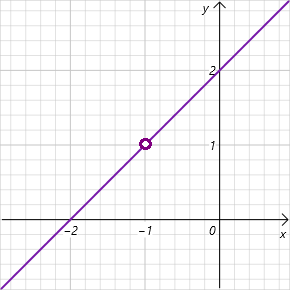
\includegraphics[width=\textwidth]
    {../Mathematik_1/Bilder/grenzwerte_hebbare_definitionsluecke.png}
  \end{minipage}
  \begin{minipage}{0.67\textwidth}
    An der Stelle \(x_0=-1\) ist kein Funktionswert definiert. Die
    Funktionswerte in der Umgebung n�hern sich jedoch von beiden Seiten
    dem Wert \(1\).

    Daher existiert der Grenzwert
    \[
    \lim_{x\to-1}f(x)=1.
    \]

    Die Definitionsl�cke k�nnte durch die Festlegung \(f(-1)=1\)
    geschlossen werden. Im folgenden Abschnitt wird sich zeigen, dass die
    so erg�nzte Funktion an dieser Stelle stetig ist.
  \end{minipage}
\end{exabox}


Der Grenzwert beschreibt somit das Verhalten der Funktion
\emph{in der Umgebung} von \(x_0\), nicht den Funktionswert an \(x_0\)
selbst.

Ein Grenzwert muss allerdings nicht existieren.

\begin{exabox}{Wenn kein Grenzwert existiert}{ }
  \begin{minipage}{0.3\textwidth}
    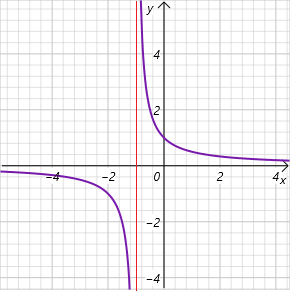
\includegraphics[width=\textwidth]
    {../Mathematik_1/Bilder/grenzwerte_polstelle_vorzeichenwechsel.png}
  \end{minipage}
  \begin{minipage}{0.67\textwidth}
    Bei einer Ann�herung an \(x_0\) zeigen die Funktionswerte von links
    und von rechts kein gemeinsames endliches Verhalten.

    In der dargestellten Situation gilt
    \[
    f(x)\to-\infty
    \quad\textnormal{f�r }x\to x_0^-,
    \]
    w�hrend
    \[
    f(x)\to+\infty
    \quad\textnormal{f�r }x\to x_0^+.
    \]

    Ein gemeinsamer endlicher Grenzwert f�r \(x\to x_0\) existiert daher
    nicht.
  \end{minipage}
\end{exabox}


\subsubsection*{Die pr�zise Bedeutung eines Funktionsgrenzwerts}

Auch beim Funktionsgrenzwert l�sst sich die Vorstellung �beliebig nahe�
mathematisch pr�zisieren.

Die Zahl \(\varepsilon>0\) beschreibt wieder einen beliebig kleinen
Abstand vom Grenzwert \(L\). Nun wird jedoch nicht ein hinreichend gro�er
Index gesucht, sondern eine hinreichend kleine Umgebung der Stelle
\(x_0\). Ihre Gr��e wird durch \(\delta>0\) beschrieben.

\begin{defbox}{Grenzwert einer Funktion}{ }
Sei \(f:D\to\mathbb R\) und \(x_0\) ein H�ufungspunkt von \(D\).
Dann bedeutet
\[
\lim_{x\to x_0}f(x)=L,
\]
dass
\[
\forall\,\varepsilon>0\;
\exists\,\delta>0\;
\forall\,x\in D:
\qquad
0<|x-x_0|<\delta
\Rightarrow
|f(x)-L|<\varepsilon.
\]

\end{defbox}

  \begin{minipage}{0.4\textwidth}
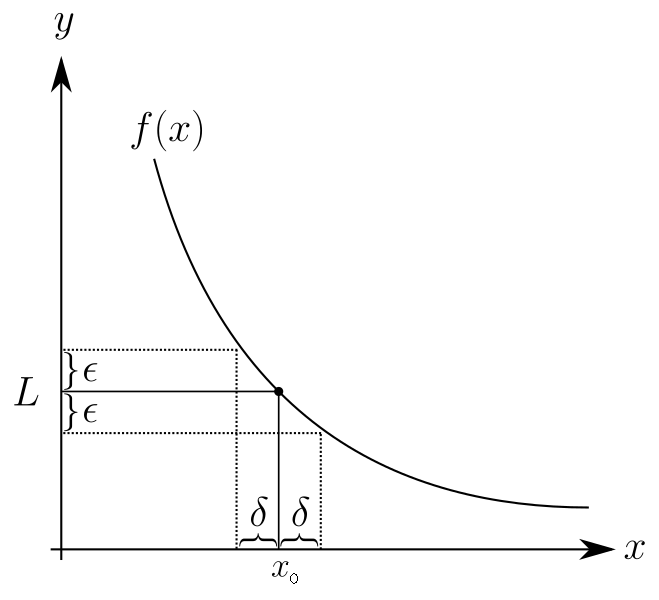
\includegraphics[width=\textwidth]
{../Mathematik_1/Bilder/grenzwerte_definition_epsilon_delta.png}
  \end{minipage}
  \begin{minipage}{0.6\textwidth}
Die Bedingung
\[
0<|x-x_0|<\delta
\]
bedeutet, dass \(x\) hinreichend nahe bei \(x_0\), aber nicht gleich
\(x_0\) liegt. F�r alle solchen \(x\) sollen die zugeh�rigen
Funktionswerte den vorgegebenen Abstand
\[
|f(x)-L|<\varepsilon
\]
vom Grenzwert \(L\) einhalten.

Damit wird auch formal sichtbar, dass der Funktionswert \(f(x_0)\) f�r
die Existenz und den Wert des Grenzwerts zun�chst keine Rolle spielt.
\end{minipage}


\subsubsection*{Die Verbindung zwischen Folgen und Funktionsgrenzwerten}

Die zuvor eingef�hrten Zahlenfolgen erm�glichen eine weitere anschauliche
Interpretation des Funktionsgrenzwerts.

Eine Folge von Stellen
\[
x_1,x_2,x_3,\ldots
\]
kann sich der Stelle \(x_0\) ann�hern:
\[
x_n\to x_0,
\qquad
x_n\neq x_0.
\]
Wird diese Folge in die Funktion eingesetzt, entsteht eine neue Folge
von Funktionswerten
\[
f(x_1),f(x_2),f(x_3),\ldots
\]

Existiert der Funktionsgrenzwert
\[
\lim_{x\to x_0}f(x)=L,
\]
so n�hern sich f�r jede solche Ann�herung an \(x_0\) auch die
Funktionswerte demselben Wert \(L\):
\[
x_n\to x_0
\qquad\Longrightarrow\qquad
f(x_n)\to L.
\]

Damit wird deutlich, weshalb Zahlenfolgen f�r den Grenzwertbegriff von
Funktionen n�tzlich sind: Eine Folge beschreibt einen m�glichen
schrittweisen Weg, sich einer Stelle \(x_0\) zu n�hern. Ein
Funktionsgrenzwert existiert nur dann, wenn das Ergebnis nicht davon
abh�ngt, auf welche Weise diese Ann�herung erfolgt.

F�hren zwei unterschiedliche Ann�herungen an dieselbe Stelle dagegen zu
unterschiedlichen Grenzwerten der Funktionswerte, so kann kein
gemeinsamer Funktionsgrenzwert existieren.


\subsubsection*{Einseitige Grenzwerte}

Bei Funktionen mit reellem Definitionsbereich kann eine Stelle \(x_0\)
von zwei Richtungen angen�hert werden. Eine Ann�herung kann ausschlie�lich
mit Werten \(x<x_0\) oder ausschlie�lich mit Werten \(x>x_0\) erfolgen.

Dies f�hrt zum \textbf{linksseitigen Grenzwert}
\[
\lim_{x\to x_0^-}f(x)
\]
und zum \textbf{rechtsseitigen Grenzwert}
\[
\lim_{x\to x_0^+}f(x).
\]

Ein gemeinsamer Grenzwert
\[
\lim_{x\to x_0}f(x)
\]
existiert genau dann, wenn beide einseitigen Grenzwerte existieren und
�bereinstimmen.

\begin{exabox}{Einseitige Grenzwerte}{ }
  \begin{minipage}{0.3\textwidth}
    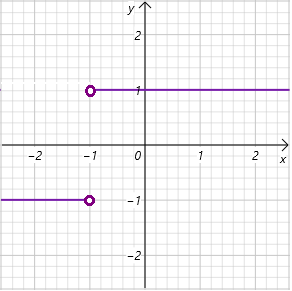
\includegraphics[width=\textwidth]
    {../Mathematik_1/Bilder/grenzwerte_einseitig_sprungstelle.png}
  \end{minipage}
  \begin{minipage}{0.67\textwidth}
    F�r die dargestellte Funktion gilt
    \[
    \lim_{x\to-1^-}f(x)=-1,
    \qquad
    \lim_{x\to-1^+}f(x)=1.
    \]
    Beide einseitigen Grenzwerte existieren, stimmen aber nicht �berein.
    Daher existiert kein gemeinsamer Grenzwert
    \[
    \lim_{x\to-1}f(x).
    \]
  \end{minipage}
\end{exabox}


\noindent\textbf{Bemerkungen:}
\begin{itemize}
  \item F�r einen Grenzwert an einer Stelle \(x_0\) m�ssen Punkte des
  Definitionsbereichs existieren, die beliebig nahe an \(x_0\) liegen
  und von \(x_0\) verschieden sind. Eine solche Stelle hei�t
  \textbf{H�ufungspunkt} des Definitionsbereichs.

  \item An Randpunkten des Definitionsbereichs ist gegebenenfalls nur
  eine einseitige Ann�herung m�glich.

  \item F�r \(x\to\infty\) beziehungsweise \(x\to-\infty\) wird das
  asymptotische Verhalten einer Funktion durch
  \textbf{uneigentliche Grenzwerte} beschrieben.
\end{itemize}


\subsubsection*{Grenzwerte von Funktionen berechnen}

Wie bei Zahlenfolgen werden Grenzwerte von Funktionen in praktischen
Berechnungen normalerweise nicht unmittelbar mithilfe der formalen
Definition bestimmt. Stattdessen werden bekannte Grenzwerte,
Grenzwerts�tze und geeignete Umformungen verwendet.

\begin{theorembox}{Grenzwerts�tze f�r Funktionen}{ }
Seien \(f,g:D\to\mathbb R\) mit
\[
\lim_{x\to x_0}f(x)=a,
\qquad
\lim_{x\to x_0}g(x)=b.
\]
Dann gilt f�r \(c\in\mathbb R\):
\[
\begin{array}{rcl}
\displaystyle
\lim_{x\to x_0}c\,f(x)
&=&ca,\\[1.5ex]

\displaystyle
\lim_{x\to x_0}\bigl(f(x)+g(x)\bigr)
&=&a+b,\\[1.5ex]

\displaystyle
\lim_{x\to x_0}\bigl(f(x)-g(x)\bigr)
&=&a-b,\\[1.5ex]

\displaystyle
\lim_{x\to x_0}f(x)g(x)
&=&ab,\\[1.5ex]

\displaystyle
\lim_{x\to x_0}\frac{f(x)}{g(x)}
&=&\frac ab
\qquad\textnormal{falls }b\neq0.
\end{array}
\]
\end{theorembox}


Besonders einfach ist die Situation bei Funktionen, deren Funktionsterme
an der betrachteten Stelle ohne Problem ausgewertet werden k�nnen.

\begin{exabox}{Direktes Einsetzen}{ }
F�r
\[
f(x)=\frac{x^2+7}{e^x}
\]
ergibt sich an der Stelle \(x_0=2\)
\[
\lim_{x\to2}\frac{x^2+7}{e^x}
=
\frac{2^2+7}{e^2}
=
\frac{11}{e^2}.
\]
\end{exabox}

Interessanter wird der Grenzwert, wenn direktes Einsetzen zun�chst zu
einem unbestimmten Ausdruck f�hrt.

\begin{exabox}{Eine hebbare Definitionsl�cke}{ }
F�r
\[
\lim_{x\to1}\frac{x^2-1}{x-1}
\]
ergibt direktes Einsetzen zun�chst den Ausdruck \(0/0\). Dieser Ausdruck
ist kein Grenzwert und enth�lt f�r sich genommen noch keine Information
�ber das tats�chliche Verhalten der Funktion.

F�r \(x\neq1\) l�sst sich jedoch faktorisieren:
\[
\frac{x^2-1}{x-1}
=
\frac{(x-1)(x+1)}{x-1}
=
x+1.
\]
Da beim Grenzwert \(x=1\) selbst nicht eingesetzt werden muss, folgt
\[
\lim_{x\to1}\frac{x^2-1}{x-1}
=
\lim_{x\to1}(x+1)
=
2.
\]
\end{exabox}

Dieses Beispiel wird f�r die Differentialrechnung von besonderer
Bedeutung sein: Auch bei der Definition der Ableitung entsteht zun�chst
ein Quotient, dessen Z�hler und Nenner gegen \(0\) streben. Der
Grenzwertbegriff erm�glicht es, trotzdem eine wohldefinierte lokale
�nderungsrate zu erhalten.


\begin{exabox}{Ein einseitiger Grenzwert}{ }
F�r
\[
f(x)=\frac{x}{|x|}
\]
gilt f�r \(x<0\)
\[
\frac{x}{|x|}=-1,
\]
w�hrend f�r \(x>0\)
\[
\frac{x}{|x|}=1
\]
gilt. Daher folgen die einseitigen Grenzwerte
\[
\lim_{x\to0^-}\frac{x}{|x|}=-1,
\qquad
\lim_{x\to0^+}\frac{x}{|x|}=1.
\]
Da sie verschieden sind, existiert kein gemeinsamer Grenzwert f�r
\(x\to0\).
\end{exabox}


\subsubsection*{Grenzwerte f�r \(x\to\infty\)}

Grenzwerte werden nicht nur in der Umgebung einer endlichen Stelle
betrachtet. Auch das bereits bekannte asymptotische Verhalten von
Funktionen l�sst sich mit der Grenzwertschreibweise ausdr�cken.

F�r rationale Funktionen
\[
f(x)=\frac{p(x)}{q(x)}
\]
wird das Verhalten f�r gro�e \(|x|\) durch die h�chsten Potenzen in
Z�hler und Nenner bestimmt.

\begin{theorembox}{Grenzwerte rationaler Funktionen f�r \(x\to\infty\)}{ }
Es seien \(p\) und \(q\) Polynome mit Grad \(n\) beziehungsweise \(m\)
und Leitkoeffizienten \(a_n\) beziehungsweise \(b_m\). Dann gilt
\[
\lim_{x\to\infty}\frac{p(x)}{q(x)}
=
\begin{cases}
0, & n<m,\\[1ex]
\dfrac{a_n}{b_m}, & n=m,\\[2ex]
\infty, & n>m\textnormal{ und }a_nb_m>0,\\[1ex]
-\infty, & n>m\textnormal{ und }a_nb_m<0.
\end{cases}
\]
\end{theorembox}

Weitere h�ufig auftretende asymptotische Grenzwerte sind:

\begin{theorembox}{Wichtige Grenzwerte f�r \(x\to\infty\)}{ }
\begin{itemize}
  \item F�r \(a>0\):
  \[
  x^a\to\infty,
  \qquad
  \frac1{x^a}\to0.
  \]

  \item F�r \(0<q<1\) und \(a\in\mathbb R\):
  \[
  q^x\to0,
  \qquad
  q^x x^a\to0.
  \]

  \item F�r \(q>1\) und \(a\in\mathbb R\):
  \[
  \frac{q^x}{x^a}\to\infty.
  \]

  \item F�r \(a>0\):
  \[
  \frac{\ln(x)}{x^a}\to0.
  \]
\end{itemize}
\end{theorembox}


\subsection*{Grenzwerte als Grundlage lokaler Eigenschaften}

Der Grenzwertbegriff erm�glicht es, das Verhalten einer Funktion in der
unmittelbaren Umgebung einer Stelle zu beschreiben. Dabei werden zwei
Gr��en zun�chst bewusst voneinander getrennt:
\[
\lim_{x\to x_0}f(x)
\qquad\textnormal{und}\qquad
f(x_0).
\]

Der erste Ausdruck beschreibt das Verhalten der Funktionswerte
\emph{in der Umgebung} von \(x_0\). Der zweite Ausdruck bezeichnet den
tats�chlichen Funktionswert \emph{an der Stelle} \(x_0\).

Damit entsteht unmittelbar eine neue Frage: Was bedeutet es, wenn beide
Werte �bereinstimmen?

\[
\lim_{x\to x_0}f(x)=f(x_0).
\]

Diese �bereinstimmung f�hrt zum Begriff der
\textbf{Stetigkeit} (\emph{continuity}). Anschaulich bedeutet sie, dass
sich das Verhalten der Funktion in der Umgebung ohne Sprung oder L�cke an
den tats�chlichen Funktionswert anschlie�t.

Der Grenzwertbegriff erm�glicht anschlie�end noch einen weiteren Schritt.
Bei der Differentialrechnung wird untersucht, ob sich nicht nur
Funktionswerte, sondern auch Differenzenquotienten einem festen Wert
ann�hern. Dieser Grenzwert f�hrt zur Ableitung und damit zur lokalen
�nderungsrate einer Funktion.

Grenzwerte bilden damit die begriffliche Grundlage f�r die beiden
zentralen lokalen Eigenschaften der folgenden Abschnitte:
\[
\text{Grenzwert}
\quad\longrightarrow\quad
\text{Stetigkeit}
\quad\longrightarrow\quad
\text{Differenzierbarkeit}.
\]

 \newpage % Folgen und Grenzwerte von Funktionen
\setcounter{exercise}{0} 
\ifintegriereaufgaben
\section*{Folgen und Grenzwerte Aufgaben}\label{MA1-grenzwerte-von-folgen-und-funktionen-aufgaben}

	Regeln und Beispiele, die zur Bearbeitung der Aufgaben hilfreich sind, finden Sie im Skript\wennreferenzvorhanden{MA1-grenzwerte-von-folgen-und-funktionen}{ (Abschnitt \abschnittsverweis{MA1-grenzwerte-von-folgen-und-funktionen})} und, falls Sie nicht weiterkommen, schauen Sie \hyperref[MA1-grenzwerte-von-folgen-und-funktionen-loesungen]{hier}.
\else 
\section{Folgen und Grenzwerte Aufgaben}\label{MA1-grenzwerte-von-folgen-und-funktionen-aufgaben}

	Regeln und Beispiele, die zur Bearbeitung der Aufgaben hilfreich sind, finden Sie im Skript und, falls Sie nicht weiterkommen, schauen Sie \hyperref[MA1-grenzwerte-von-folgen-und-funktionen-loesungen]{hier}.
\fi 

\begin{exercisebox}[Folgen]
	Betrachten Sie einen Kreis und zeichnen Sie die Fl�che $A_3$ des durch den Kreis einbeschriebenen regelm��igen Dreiecks ein, dann die Fl�che $A_6$ eines regelm��iges Sechsecks, $A_{12}$ eines regelm��igen Zw�lfecks usw. 
	\begin{itemize}
		\item Konvergiert die Folge der Fl�cheninhalte? 
		\item Wenn ja, wie lautet der Grenzwert? 
	\end{itemize}
\end{exercisebox}

\begin{exercisebox}[Grenzwerte]
	\begin{itemize}
		\item[(a)] �bersetzen Sie die folgende Aussage: \newline Es sei $(a_n)_{n\in\mathbb N^+}$ und es gelte: \( \forall\, \varepsilon > 0 \; \exists\, n_\varepsilon \in \mathbb N \; \forall\, n\geq n_\varepsilon  \; |a_n - a| < \varepsilon \quad (*)\)
		\item[(b)] Erf�llt die Folge $(a_n)_{n\in \mathbb N}$ mit \( a_n = \dfrac{2n}{n+4}\) die Eigenschaft $(*)$? Falls ja, wie lautet $n_\varepsilon$ bei gegebenem $\varepsilon > 0$?
	\end{itemize}
\end{exercisebox}

\begin{exercisebox}[Grenzwerts�tze]
	Geben Sie f�r $c=0, \; c=1, \; c=\infty$ jeweils Folgen $(a_n)_{n\in \mathbb N} $ und $(b_n)_{n\in \mathbb N}$ an, so dass 
	\begin{eqnarray*} 
		\lim\limits_{n\to \infty} \left( a_n \cdot b_n\right) = c \quad \textnormal{mit}\; a_n \to \infty, b_n\to 0 \; \textnormal{f\"ur } n\to \infty\,, \\
		\lim\limits_{n\to \infty} \frac{ a_n }{ b_n} =  c \quad \textnormal{mit}\; a_n \to 0, b_n\to 0 \; \textnormal{f\"ur } n\to \infty\,, 
	\end{eqnarray*}
\end{exercisebox}

\begin{exercisebox}[Grenzwerte von Folgen]
	Bestimmen Sie ob die folgenden Grenzwerte existieren und berechnen Sie sie gegebenenfalls. 
  \begin{eqnarray*}
		  (a)\; \lim\limits_{n\to \infty} \displaystyle{\frac{(n+1)^2-n^2 }{n}} \quad 
		  (b)\; \displaystyle{\lim\limits_{n\to \infty}} \displaystyle{\frac{9\, n^2+n+1}{3n^3 +1}} \quad
		  (c)\; \lim\limits_{n\to \infty} \displaystyle{\frac{1 + 2 + \cdots + n }{n^2}} \quad 
		  (d)\; \lim\limits_{n\to \infty} \left( \sqrt{n+1} - \sqrt{n}\right) 
	  \end{eqnarray*}
		  %(d)\; \displaystyle{\lim\limits_{n\to \infty}} \displaystyle{\frac{1+2^2 + \cdots + n^2}{n^3}} \\
Hinweis zu $(c)$: Es gilt 
	$\displaystyle{\sum\limits_{k=1}^n k} =\displaystyle{\frac12}\cdot n \cdot (n+1)$
  \end{exercisebox}

\begin{exercisebox}[Grenzwerte von Folgen]
	�berpr�fen Sie, ob die Zahlenfolge $\{ f_n\}_{n\in\mathbb N^+}$ konvergiert und berechnen Sie ggf. den Grenzwert: 
	\[ f_1=0, \; f_{n+1} = \frac13 ( f_n +1)\,.\]
\end{exercisebox}

\begin{exercisebox}[Grenzwerte von Funktionen]
	Bestimmen Sie ob die folgenden Grenzwerte existieren und berechnen Sie sie gegebenenfalls.
  \begin{eqnarray*}
	  \begin{array}{llll}
	  (a)\; \lim\limits_{x\to\infty} \dfrac{-x^2+1}{x^3+2x^2+x} &\quad 
	  (b)\; \lim\limits_{x\to-\infty} \dfrac{-(x+1)^2}{2x^2-x+1} &\quad 
	  (c)\; \lim\limits_{x\to-\infty} \dfrac{2x^3+x^2-x}{-x^2+4} &\quad
	  (d)\; \lim\limits_{x\to \infty} \left( 2^{-x}\cdot x^4 \right) \\
	(e)\; \lim\limits_{x\to \infty} \dfrac{ \left( \ln(x)\right)^3}{x^2} &\quad
	(f)\; \lim\limits_{x\downarrow 0} \dfrac{ 2^{\frac1x}}{\ln(x)} &\quad
	(g)\; \lim\limits_{x\to 0} \dfrac{ x}{|x|} &\quad
	(h)\; \lim\limits_{x\to 0} \dfrac{\cos(x)}{x}
	  %(f)\; \lim\limits_{x\to \infty} \left( 2- \frac{1}{(x+3)^2}\right) &\quad
	  %(g)\; \lim\limits_{x\to \infty} \left( -\frac{1}{2x}+ 3\right) &\quad
	  %(h)\; \lim\limits_{x\to \infty} \frac{1}{\sqrt{x+1}} &\quad 
	  %(i)\; \lim\limits_{x\to \infty} \frac{1}{\sqrt{x}}+1 
  \end{array}
  \end{eqnarray*}

\end{exercisebox}

%\begin{exercisebox}[Teleskopsumme]
%\end{exercisebox}

%\begin{exercisebox}[Konvergenz Binomialreihe $e$]
%\end{exercisebox}
%
%\begin{exercisebox}[Konvergenz Potenzreihe $\exp$]
%\end{exercisebox}
%
%\begin{exercisebox}[Harmonische Reihe]
%\end{exercisebox}
%
%\begin{exercisebox}[Riemann Integral]
%\end{exercisebox}

%\begin{theorembox}[Konvergenz Reihe]
%  Reihe mit alternierender Nullfolge ist konvergent (nicht absolut konvergent). (Leibnitz Kriterizm)
%\end{theorembox}
%
%\begin{theorembox}[Teleskop Summe]
%  Reihe mit alternierender Nullfolge ist konvergent (nicht absolut konvergent). (Leibnitz Kriterizm)
%\end{theorembox}
%
%\begin{theorembox}[absolute Konvergenz]
%  absolut konvergene Reihen (Reihenfolge der Glieder egal): wenn die Summe �ber die Betr�ge der Koeffizienten konvergiert.  
%\end{theorembox}
%
%\begin{theorembox}[Potenzreihen stellen Funktionen dar]
%  Konvergenzradius: f�r welche $x$ konvergiert die Potenzreihe?
%\end{theorembox}
%
%\begin{theorembox}[Funktionenr�ume, Betrag, Metrik]
%	Abstandsbegriffe, Energie Physik
%\end{theorembox}
%
%\begin{theorembox}[Lipschitz-Stetigkeit]
%\end{theorembox}
%
%\begin{theorembox}[Mittelwertsatz]
%\end{theorembox}
%
%\begin{theorembox}[Chauchy-Folge]
%\end{theorembox}
%\begin{theorembox}[Vollst�ndigkeit]
%\end{theorembox}
%\begin{theorembox}[Banachscher Fixpunktsatz]
%\end{theorembox}
%
%\begin{theorembox}[Iterationsverfahren]
%  Was wollen wir �ber das Iterationsverfahren wissen?
%  \begin{itemize}
%	  \item Konvergiert das Verfahren �berhaupt? $\Rightarrow $ Banachscher Fixpunktsatz
%	  \item Gegen welchen Wert konvergiert es? $\Rightarrow$ Fixpunkt
%	  \item Wie schnell konvergiert das Verfahren? $\Rightarrow$ Konvergenzordung
%  \end{itemize}
%\end{theorembox}
 \newpage 
\setcounter{satz}{0} \setcounter{def}{0} \setcounter{exa}{0}  
\section{Stetigkeit und Differenzierbarkeit}\label{MA1-stetigkeit-und-differenzierbarkeit}

\begin{table}[H]
  \centering
  \begin{tabularx}{\textwidth}{p{0.9\textwidth} p{0.1\textwidth}}
    \toprule
    \multicolumn{2}{c}{\textbf{�bersicht �ber Lernziele und Voraussetzungen}}\\
    \midrule
    \textbf{Lernziele} & \\[.5\normalbaselineskip]
    \tabitem Stetigkeit erkl�ren und untersuchen &\\
    \tabitem Parameter so bestimmen, dass eine st�ckweise definierte
    Funktion stetig ist &\\
    \tabitem den Differenzenquotienten als mittlere �nderungsrate interpretieren &\\
    \tabitem die Ableitung als lokale �nderungsrate interpretieren &\\
    \tabitem Differenzierbarkeit �ber den Grenzwert des Differenzenquotienten erkl�ren und untersuchen &\\
    \tabitem den Zusammenhang zwischen Differenzierbarkeit, Stetigkeit und lokaler Linearit�t erl�utern &\\
    \midrule
    \textbf{Voraussetzungen} & \\[.5\normalbaselineskip]
\tabitem Steigung linearer Funktionen & \abschnittsverweis{MA1-eigenschaften-von-funktionen}\\
\tabitem St�ckweise definierte Funktionen & \abschnittsverweis{MA1-eigenschaften-von-funktionen}\\
    \tabitem st�ckweise definierte Funktionen & \abschnittsverweis{MA1-lineare-funktionen}\\
    \tabitem Grenzwerte von Funktionen und einseitige Grenzwerte
    & \abschnittsverweis{MA1-grenzwerte-von-folgen-und-funktionen}\\
    \bottomrule
  \end{tabularx}
\end{table}

\ifintegriereaufgaben
\noindent �bungsaufgaben zum Thema:
\hyperref[MA1-stetigkeit-und-differenzierbarkeit-aufgaben]{Aufgaben}
\vspace{0.3cm}
\hrule
\fi


\subsection{Was ist Stetigkeit?}

Der Grenzwert
\[
\lim_{x\to x_0}f(x)
\]
beschreibt, welchem Wert sich die Funktionswerte n�hern, wenn sich \(x\)
der Stelle \(x_0\) n�hert. Dabei spielt der tats�chliche Funktionswert
\(f(x_0)\) zun�chst keine Rolle.

F�r eine Funktion, die an \(x_0\) definiert ist, k�nnen daher zwei Werte
miteinander verglichen werden:
\[
\lim_{x\to x_0}f(x)
\qquad\textnormal{und}\qquad
f(x_0).
\]

Stimmen beide �berein, so schlie�t sich das Verhalten der Funktion in der
Umgebung von \(x_0\) ohne L�cke oder Sprung an den Funktionswert an.
Genau diese Eigenschaft beschreibt die \textbf{Stetigkeit}
(\emph{continuity}).


\begin{defbox}{Stetigkeit in \(x_0\)}{ }
Eine Funktion \(f:D\to\mathbb R\) ist an einer Stelle \(x_0\in D\)
\textbf{stetig}, wenn
\[
\lim_{x\to x_0}f(x)=f(x_0).
\]
\end{defbox}

F�r Stetigkeit m�ssen damit drei Dinge zusammenpassen: Die Funktion muss
an \(x_0\) definiert sein, der Grenzwert f�r \(x\to x_0\) muss existieren
und dieser Grenzwert muss mit dem Funktionswert \(f(x_0)\) �bereinstimmen.

Anschaulich bedeutet Stetigkeit, dass kleine �nderungen von \(x\) in der
N�he von \(x_0\) nur kleine �nderungen von \(f(x)\) hervorrufen. Der Graph
besitzt dort insbesondere weder einen Sprung noch eine L�cke.


\begin{exabox}{\(\sin:x\mapsto\sin(x)\) ist stetig}{ }
  \begin{minipage}{0.5\textwidth}
    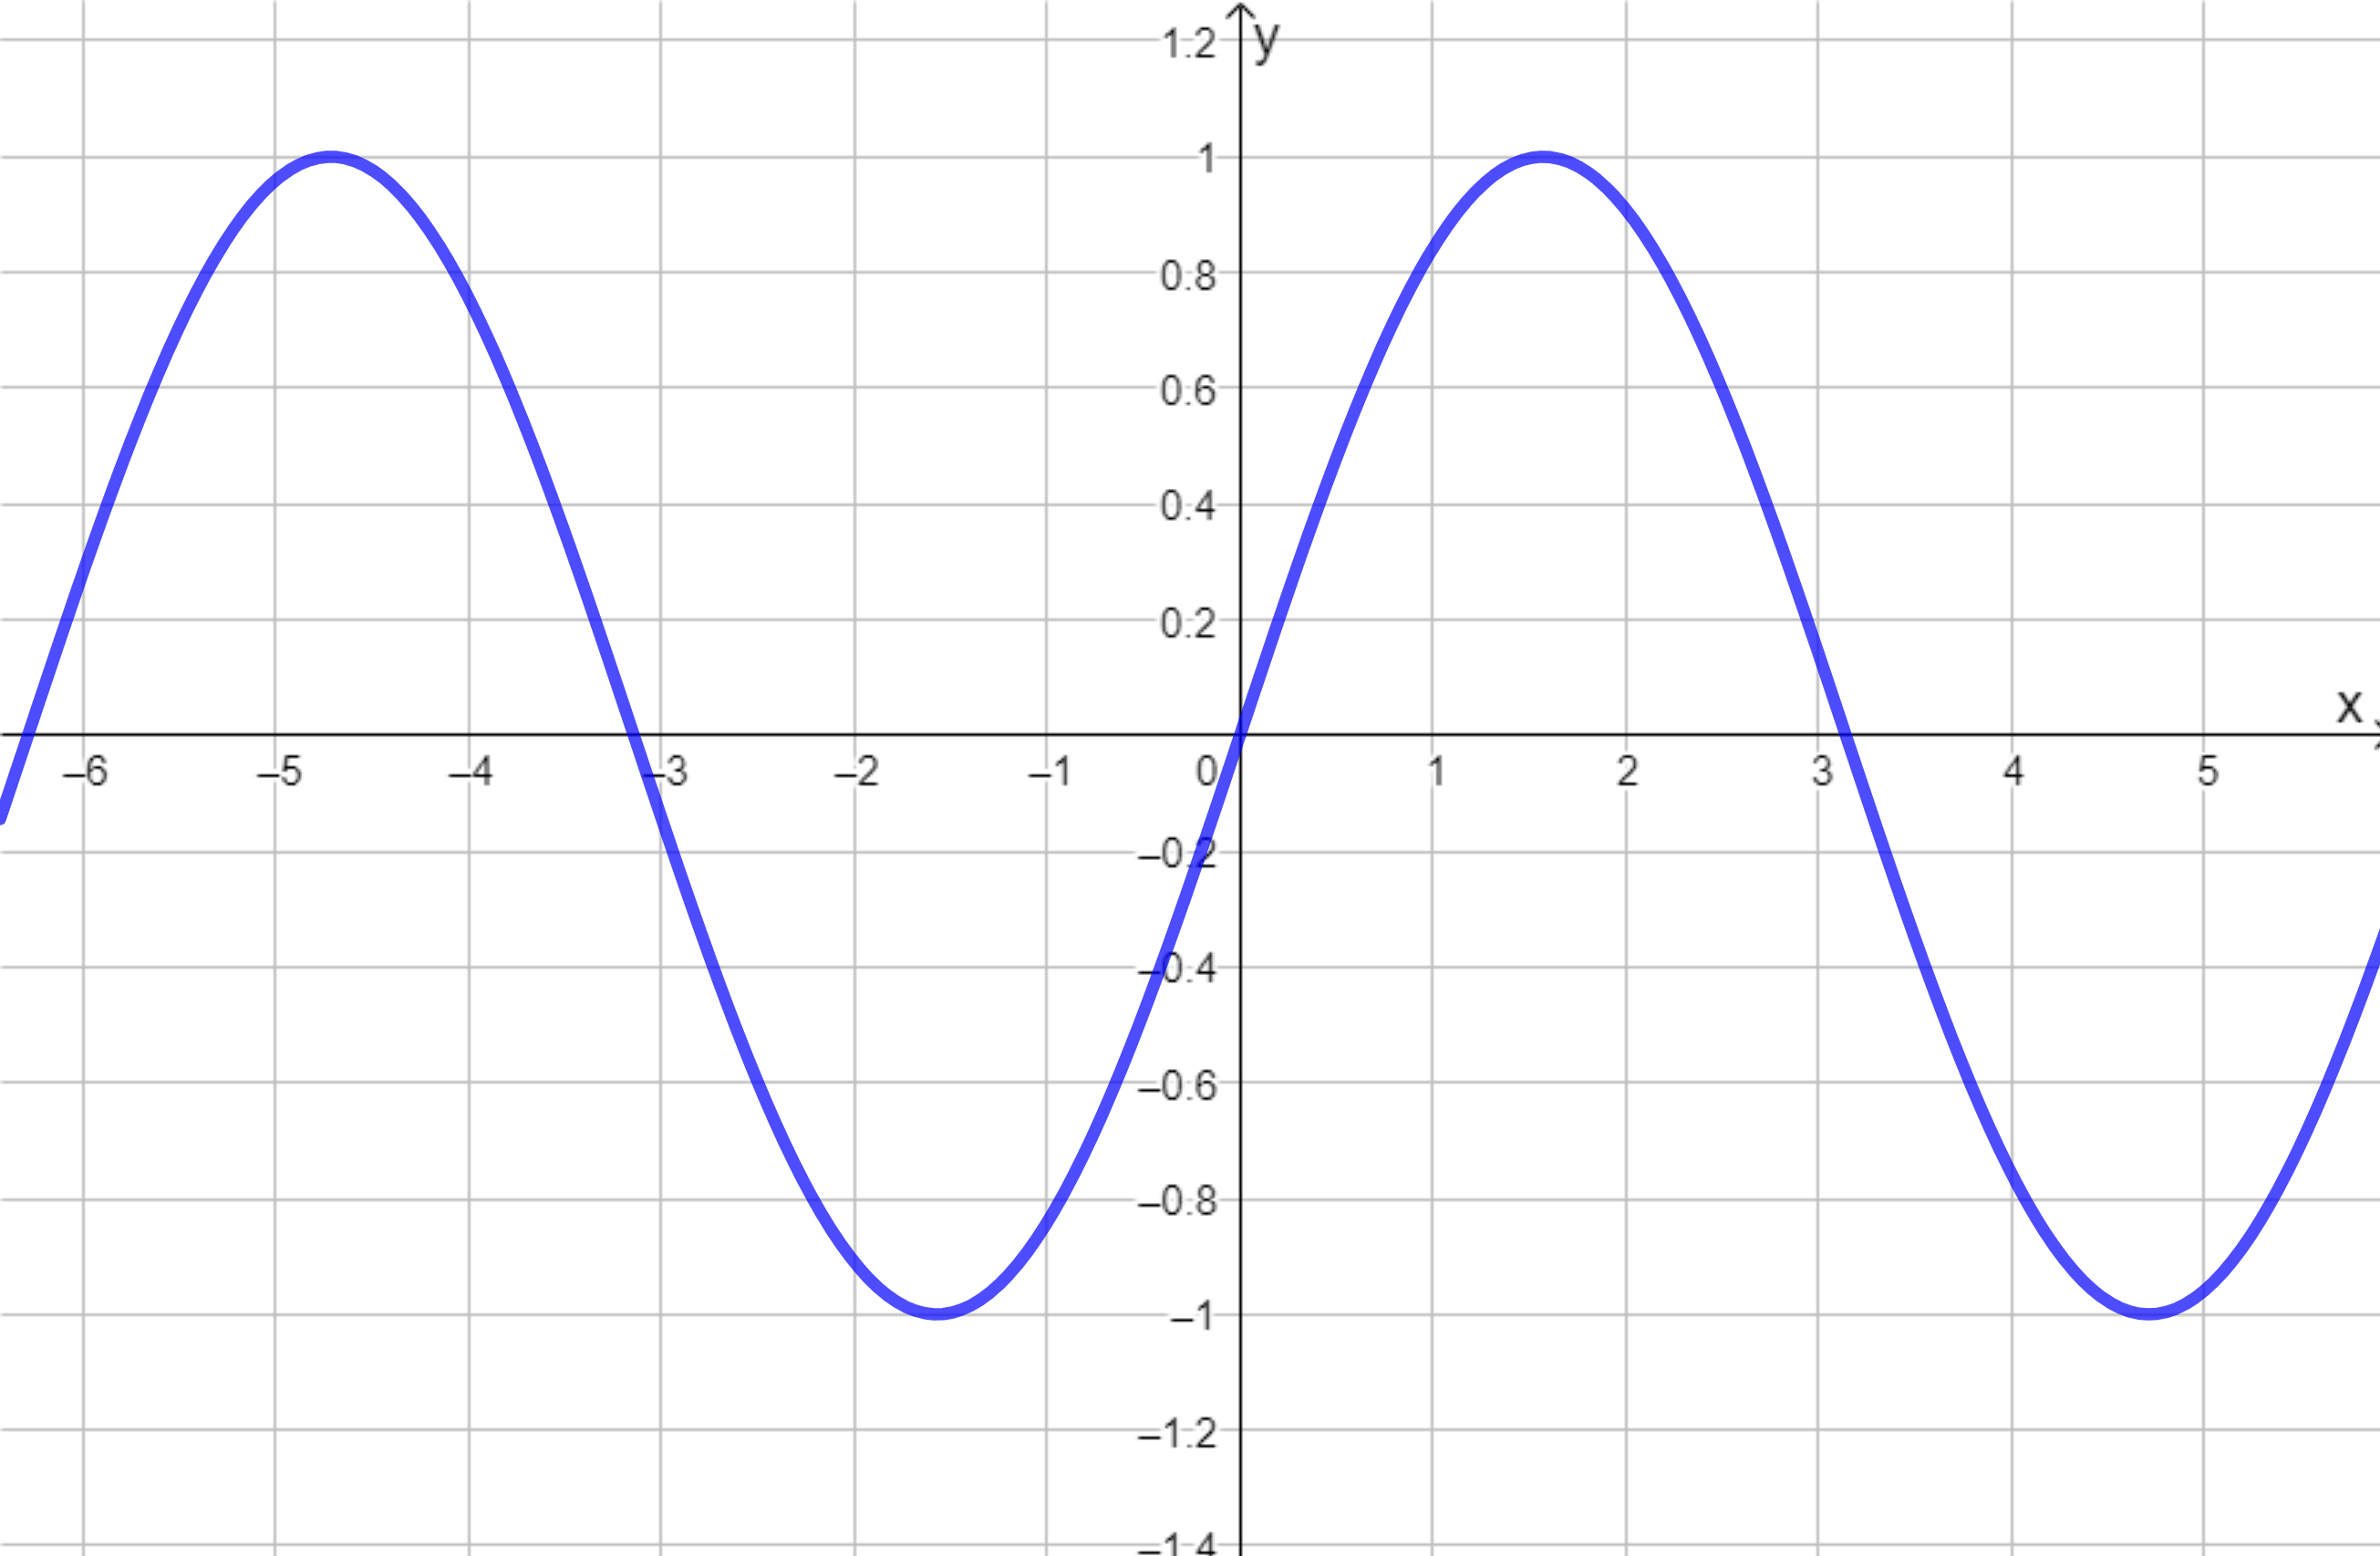
\includegraphics[width=\textwidth]
    {../Mathematik_1/Bilder/stetigkeit_sinusfunktion.png}
  \end{minipage}
  \begin{minipage}{0.45\textwidth}
    Der Graph der Sinusfunktion besitzt weder Spr�nge noch L�cken.

    Anschaulich l�sst er sich zeichnen, ohne den Stift abzusetzen.
    Diese Vorstellung ist f�r viele reelle Funktionen hilfreich, ersetzt
    aber nicht die mathematische Definition der Stetigkeit.
  \end{minipage}
\end{exabox}


\subsubsection*{Eine wichtige Konsequenz der Stetigkeit}

Eine stetige Funktion kann zwischen zwei Funktionswerten keine Werte
�berspringen. Liegen beispielsweise \(f(a)\) und \(f(b)\) auf
unterschiedlichen Seiten eines Wertes \(y\), so muss der Graph den Wert
\(y\) zwischen \(a\) und \(b\) annehmen.

Diese Eigenschaft wird durch den Zwischenwertsatz pr�zisiert.

\begin{theorembox}{Zwischenwertsatz}{ }
Es sei \(f:D\to\mathbb R\) stetig und \([a,b]\subset D\).
F�r jeden Wert \(y\) zwischen \(f(a)\) und \(f(b)\) existiert mindestens
ein \(x\in[a,b]\) mit
\[
f(x)=y.
\]
\end{theorembox}

Eine wichtige Anwendung ergibt sich f�r \(y=0\): Haben \(f(a)\) und
\(f(b)\) unterschiedliche Vorzeichen, so besitzt eine stetige Funktion
zwischen \(a\) und \(b\) mindestens eine Nullstelle.


\subsubsection*{Stetigkeit und Folgen}

Der Grenzwertbegriff wurde zun�chst mithilfe von Zahlenfolgen als
Ann�herungsprozess entwickelt. Auch Stetigkeit l�sst sich in dieser
Vorstellung unmittelbar interpretieren.

N�hert sich eine Folge von Stellen \(x_n\) einer Stelle \(x_0\), so m�ssen
sich bei einer stetigen Funktion die zugeh�rigen Funktionswerte dem
Funktionswert \(f(x_0)\) n�hern.

\begin{theorembox}{Folgenstetigkeit}{ }
Ist \(f\) in \(x_0\) stetig und gilt
\[
x_n\to x_0,
\]
so folgt
\[
f(x_n)\to f(x_0).
\]
\end{theorembox}

Bei stetigen Funktionen kann der Grenzwert damit mit der Funktion
vertauscht werden:
\[
\lim_{n\to\infty}f(x_n)
=
f\left(\lim_{n\to\infty}x_n\right)
=
f(x_0).
\]

In diesem Sinne darf bei stetigen Funktionen der Grenzwert
\emph{eingesetzt} werden.


\subsubsection*{Hebbare Definitionsl�cken}

Der Grenzwert einer Funktion kann an einer Stelle auch dann existieren,
wenn die Funktion dort selbst nicht definiert ist. In diesem Fall ist die
urspr�ngliche Funktion an dieser Stelle nicht stetig, da \(f(x_0)\) nicht
existiert.

Existiert jedoch ein endlicher Grenzwert
\[
\lim_{x\to x_0}f(x)=L,
\]
so kann die fehlende Stelle durch die Festlegung
\[
f(x_0)=L
\]
erg�nzt werden. Eine solche Definitionsl�cke hei�t
\textbf{hebbare Definitionsl�cke}; die erg�nzte Funktion hei�t
\textbf{stetige Fortsetzung}.


\begin{exabox}{Stetige Fortsetzung}{ }
Die Funktion
\[
f:\mathbb R\setminus\{0\}\to(0,\infty),
\qquad
x\mapsto e^{-1/x^2},
\]
ist im Nullpunkt nicht definiert. Es gilt jedoch
\[
\lim_{x\to0}e^{-1/x^2}=0.
\]

Die Definitionsl�cke l�sst sich daher durch den Grenzwert schlie�en.
Eine stetige Fortsetzung ist
\[
\widetilde f:\mathbb R\to[0,\infty),
\qquad
x\mapsto
\begin{cases}
e^{-1/x^2}, & x\neq0,\\
0,          & x=0.
\end{cases}
\]
\end{exabox}


\subsection{Was ist Differenzierbarkeit?}

Stetigkeit beschreibt, ob sich das Verhalten einer Funktion in der
Umgebung einer Stelle ohne Sprung oder L�cke an den dortigen
Funktionswert anschlie�t. F�r die Untersuchung lokaler Ver�nderungen
reicht diese Information jedoch noch nicht aus.

Von besonderem Interesse ist nun die Frage, \emph{wie stark} sich die
Funktionswerte ver�ndern, wenn sich \(x\) in der Umgebung einer Stelle
\(x_0\) ver�ndert.

Dazu werden zun�chst zwei Punkte des Funktionsgraphen betrachtet:
\[
P=\bigl(x_0,f(x_0)\bigr)
\qquad\textnormal{und}\qquad
Q=\bigl(x_0+h,f(x_0+h)\bigr).
\]

Die Gerade durch diese beiden Punkte ist eine Sekante. Ihre Steigung
ergibt sich aus der �nderung der Funktionswerte geteilt durch die �nderung
der Argumente:
\[
\frac{f(x_0+h)-f(x_0)}
     {(x_0+h)-x_0}
=
\frac{f(x_0+h)-f(x_0)}{h}.
\]

Dieser Ausdruck hei�t \textbf{Differenzenquotient}. Er beschreibt die
mittlere �nderungsrate von \(f\) zwischen \(x_0\) und \(x_0+h\).

Nun r�ckt der zweite Punkt immer n�her an den ersten heran. Mathematisch
entspricht dies dem Grenz�bergang
\[
h\to0.
\]
Existiert dabei ein endlicher Grenzwert des Differenzenquotienten, so
entsteht aus der mittleren �nderungsrate eine lokale oder momentane
�nderungsrate. Geometrisch n�hert sich die Sekante einer Tangente an.


\begin{defbox}{Differenzierbarkeit in \(x_0\)}{ }
Eine Funktion \(f\) hei�t an der Stelle \(x_0\)
\textbf{differenzierbar} (\emph{differentiable}), wenn der Grenzwert
\[
\lim_{h\to0}
\frac{f(x_0+h)-f(x_0)}{h}
\]
existiert.

Der Wert dieses Grenzwerts hei�t \textbf{Ableitung}
(\emph{derivative}) von \(f\) an der Stelle \(x_0\):
\[
f'(x_0)
=
\lim_{h\to0}
\frac{f(x_0+h)-f(x_0)}{h}.
\]
\end{defbox}

Die Ableitung \(f'(x_0)\) besitzt damit zwei unmittelbar miteinander
verbundene Interpretationen:

\[
\text{lokale �nderungsrate}
\qquad\longleftrightarrow\qquad
\text{Tangentensteigung}.
\]


\subsubsection*{Die Ableitungsfunktion}

Ist \(f\) nicht nur an einer einzelnen Stelle, sondern an allen Stellen
eines Bereichs differenzierbar, so kann jedem \(x\) die dortige lokale
�nderungsrate zugeordnet werden.

Dadurch entsteht aus \(f\) eine neue Funktion: die
\textbf{Ableitungsfunktion} \(f'\).

\begin{defbox}{Erste Ableitung von \(f\)}{ }
\[
f':
x\mapsto
\lim_{h\to0}
\frac{f(x+h)-f(x)}{h}.
\]

G�ngige Bezeichnungen f�r die erste Ableitung sind
\[
f',
\qquad
\frac{\mathrm df}{\mathrm dx},
\qquad
f^{(1)}.
\]

Ist die unabh�ngige Variable die Zeit \(t\), wird h�ufig auch die
Schreibweise
\[
\dot f=\frac{\mathrm df}{\mathrm dt}
\]
verwendet.
\end{defbox}

Der Definitionsbereich von \(f'\) besteht aus denjenigen Stellen des
Definitionsbereichs von \(f\), an denen \(f\) differenzierbar ist.


\begin{exabox}{Zusammenhang zwischen Funktion und Ableitung}{ }
  \begin{minipage}{0.5\textwidth}
    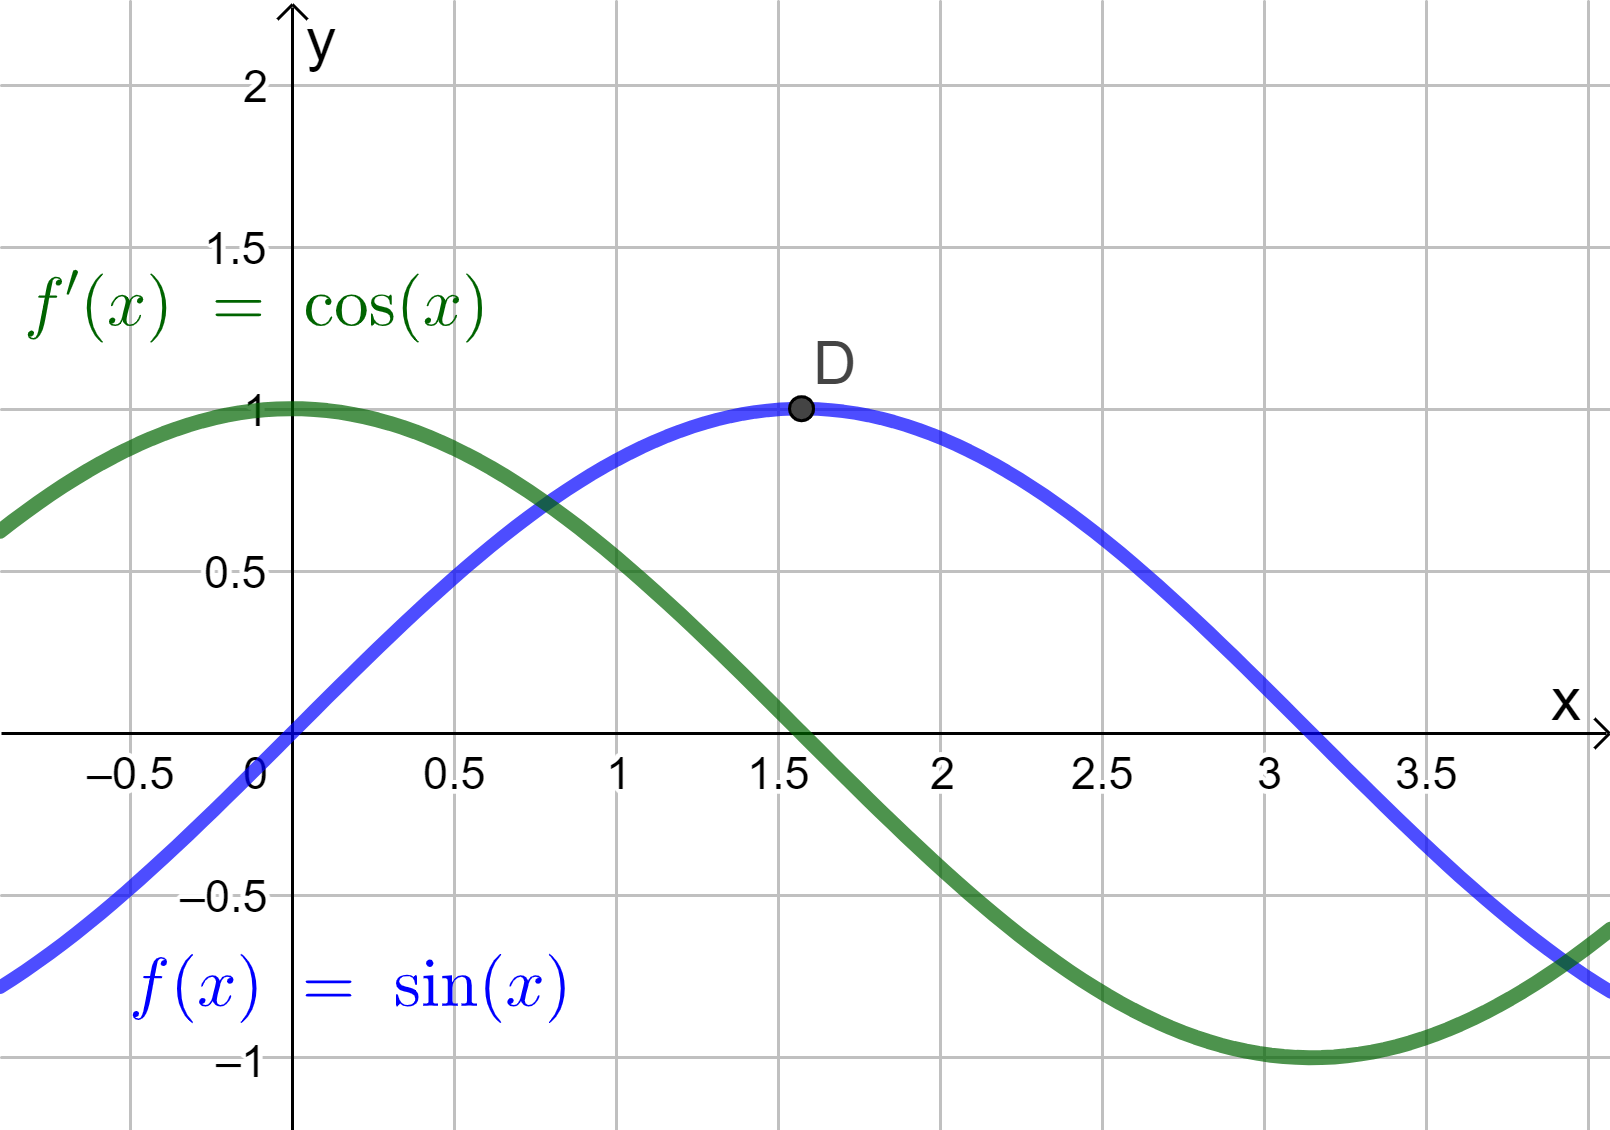
\includegraphics[width=\textwidth]
    {../Mathematik_1/Bilder/ableitung_sinus_kosinus.png}
  \end{minipage}
  \begin{minipage}{0.45\textwidth}
    Die Ableitung beschreibt die lokale �nderung von \(f\):
    \begin{itemize}
      \item W�chst \(f\), so ist \(f'\) positiv.
      \item F�llt \(f\), so ist \(f'\) negativ.
      \item Besitzt \(f\) an einer inneren Stelle ein lokales Maximum oder
      Minimum und ist dort differenzierbar, so gilt \(f'(x)=0\).
    \end{itemize}
  \end{minipage}
\end{exabox}


\subsubsection*{Differenzierbarkeit und Stetigkeit}

Differenzierbarkeit stellt eine st�rkere lokale Anforderung an eine
Funktion als Stetigkeit.

\begin{theorembox}{Differenzierbarkeit und Stetigkeit}{ }
Ist eine Funktion \(f\) an einer Stelle \(x_0\) differenzierbar, so ist
sie dort auch stetig:
\[
f\textnormal{ differenzierbar in }x_0
\quad\Longrightarrow\quad
f\textnormal{ stetig in }x_0.
\]

Die Umkehrung gilt im Allgemeinen nicht.
\end{theorembox}

Eine stetige Funktion kann also durchaus Stellen besitzen, an denen keine
eindeutige Tangentensteigung existiert. Ein besonders einfaches Beispiel
ist die Betragsfunktion.


\begin{exabox}{Stetig, aber nicht differenzierbar: \(f(x)=|x|\)}{ }
  \begin{minipage}{0.5\textwidth}
    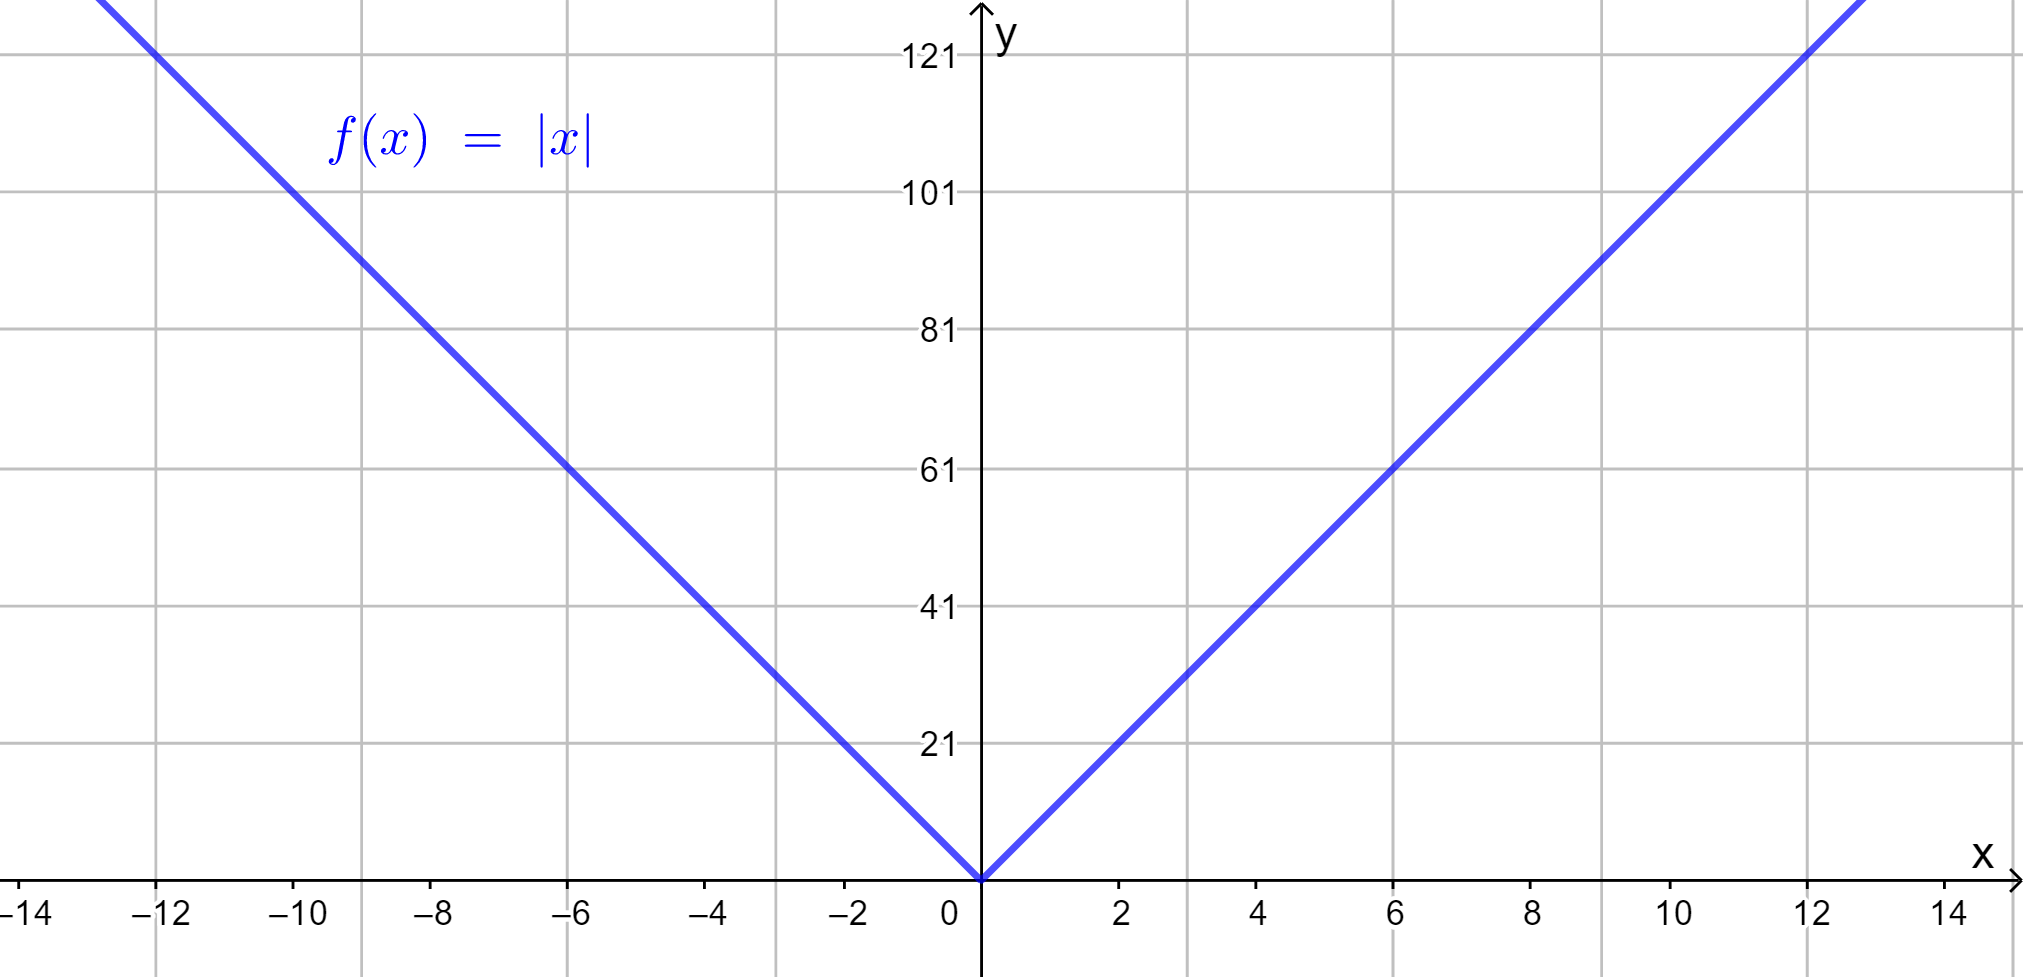
\includegraphics[width=\textwidth]
    {../Mathematik_1/Bilder/differenzierbarkeit_betragsfunktion_knick.png}
  \end{minipage}
  \begin{minipage}{0.45\textwidth}
    Die Betragsfunktion ist in \(x_0=0\) stetig. Dort besitzt ihr Graph
    jedoch einen Knick.

    F�r \(x_0=0\) lautet der Differenzenquotient
    \[
    \frac{f(0+h)-f(0)}{h}
    =
    \frac{|h|}{h}.
    \]

    Die einseitigen Grenzwerte sind
    \[
    \lim_{h\to0^-}\frac{|h|}{h}=-1,
    \qquad
    \lim_{h\to0^+}\frac{|h|}{h}=1.
    \]

    Da beide Grenzwerte verschieden sind, existiert der Grenzwert des
    Differenzenquotienten nicht. Die Betragsfunktion ist daher in
    \(x_0=0\) nicht differenzierbar.
  \end{minipage}
\end{exabox}

Das Beispiel zeigt den Unterschied zwischen beiden Begriffen besonders
deutlich: F�r Stetigkeit gen�gt es, dass sich die Funktionswerte passend
an \(f(x_0)\) anschlie�en. Differenzierbarkeit verlangt zus�tzlich, dass
sich die lokalen �nderungsraten von beiden Seiten an denselben Wert
ann�hern.


\subsection{Differenzierbarkeit als lokale Linearit�t}

Die Ableitung beschreibt nicht nur eine Steigung. Hinter der
Differenzierbarkeit steht eine weitergehende lokale Eigenschaft, die f�r
die folgenden Abschnitte von zentraler Bedeutung ist.

Ist eine Funktion in \(x_0\) differenzierbar, so l�sst sie sich in einer
hinreichend kleinen Umgebung von \(x_0\) immer besser durch eine Gerade
approximieren. Diese Eigenschaft wird als
\textbf{lokale Linearit�t} bezeichnet.

Ausgehend von \(x_0\) wird eine kleine �nderung \(h\) betrachtet. Die
zugeh�rige �nderung des Funktionswertes l�sst sich zerlegen in einen
linearen Anteil
\[
f'(x_0)h
\]
und einen verbleibenden Fehler. Differenzierbarkeit bedeutet, dass dieser
Fehler f�r \(h\to0\) gegen�ber \(h\) vernachl�ssigbar klein wird.


\begin{defbox}{Differenzierbarkeit als lokale Linearisierung}{ }
Eine Funktion \(f\) ist in \(x_0\) genau dann differenzierbar, wenn
\[
f(x_0+h)
=
f(x_0)+f'(x_0)h+r(h),
\]
wobei f�r den Rest \(r(h)\) gilt
\[
\lim_{h\to0}\frac{r(h)}{h}=0.
\]
\end{defbox}

H�ufig wird f�r einen solchen Rest auch die
\textbf{Landau-Schreibweise}
\[
r(h)=o(h)
\]
verwendet. Damit l�sst sich dieselbe Aussage kompakt als
\[
f(x_0+h)
=
f(x_0)+f'(x_0)h+o(h)
\]
schreiben.

Der entscheidende Teil dieser Darstellung ist
\[
f(x_0)+f'(x_0)h.
\]
Er beschreibt die lokale affine Approximation der Funktion.

Mit
\[
h=x-x_0
\]
ergibt sich daraus
\[
f(x)
\approx
f(x_0)+f'(x_0)(x-x_0).
\]

Die zugeh�rige Tangente an den Funktionsgraphen besitzt daher die
Gleichung
\[
t(x)
=
f(x_0)+f'(x_0)(x-x_0).
\]

Die Tangente stimmt an der Stelle \(x_0\) sowohl im Funktionswert als auch
in der Steigung mit \(f\) �berein:
\[
t(x_0)=f(x_0),
\qquad
t'(x_0)=f'(x_0).
\]

Differenzierbarkeit kann damit auf zwei eng miteinander verbundenen Wegen
verstanden werden: �ber den Grenzwert des Differenzenquotienten als
\emph{lokale �nderungsrate} und �ber die Tangente als
\emph{lokale affine Approximation} der Funktion.

Im folgenden Abschnitt werden aus dieser Definition Rechenregeln
entwickelt, mit denen Ableitungen bestimmt werden k�nnen, ohne den
Differenzenquotienten jedes Mal erneut von Grund auf untersuchen zu
m�ssen.
 \newpage % Stetigkeit und Differenzierbarkeit
\setcounter{exercise}{0} 
\ifintegriereaufgaben
\section*{Stetigkeit Aufgaben}\label{MA1-stetigkeit-und-differenzierbarkeit-aufgaben}

	Regeln und Beispiele, die zur Bearbeitung der Aufgaben hilfreich sind, finden Sie im Skript\wennreferenzvorhanden{MA1-stetigkeit-und-differenzierbarkeit}{ (Abschnitt \abschnittsverweis{MA1-stetigkeit-und-differenzierbarkeit})} und, falls Sie nicht weiterkommen, schauen Sie \hyperref[MA1-stetigkeit-und-differenzierbarkeit-loesungen]{hier}.
\else
\section{Stetigkeit Aufgaben}\label{MA1-stetigkeit-und-differenzierbarkeit-aufgaben}

	Regeln und Beispiele, die zur Bearbeitung der Aufgaben hilfreich sind, finden Sie im Skript und, falls Sie nicht weiterkommen, schauen Sie \hyperref[MA1-stetigkeit-und-differenzierbarkeit-loesungen]{hier}.
\fi 

\begin{exercisebox}[Stetigkeit]
	\begin{itemize}
		\item[(a)] Es sei $f:D \subseteq \mathbb R\to \mathbb R$ und $x_0 \in D$. Was bedeutet die folgende Aussage:
		\[ \exists \varepsilon > 0 \forall \delta > 0 \exists x\in D : |x-x_0| < \delta \land |f(x) - f(x_0)|\geq \varepsilon\,. \]
	\item[(b)] Betrachten Sie die Funktion $f:\mathbb R\to \mathbb R$ mit $f: x \mapsto \frac13 x$. Gibt es eine Stelle $x_0 \in \mathbb R$, an der die Bedingung unter $(a)$ erf�llt ist?
\end{itemize}
\end{exercisebox}


\begin{exercisebox}[Stetigkeit]
	Untersuchen Sie die Funktion $f$ mit \[f: x \mapsto \begin{cases} 1,  &\quad x \in \mathbb Q\,, \\ 0, &\quad x \in \mathbb R\setminus \mathbb Q \,,\end{cases}\] auf Stetigkeit an einer beliebigen Stelle $x_0$.
\end{exercisebox} 


\begin{exercisebox}[Stetigkeit]
	F�r welche $x\in [0,\infty)$ ist $f$ stetig?
  \begin{eqnarray*}
	  f: x\mapsto \begin{cases}
      1 \quad &x>1\\
      \frac{1}{|x|} \quad & 0 <x\leq 1\\
      0 \quad & x\leq 0\\
    \end{cases}
  \end{eqnarray*}
\end{exercisebox} 

\begin{exercisebox}[Stetigkeit]
  Bestimmen Sie $t\in \mathbb R$ so, dass die Funktion $f$ an der Stelle $x_0$ stetig ist.
  \begin{enumerate}
	  \item[(a)] Es sei $x_0=1$ und 
      $
  	  f: x\mapsto \begin{cases}
  	    x+1 \quad &x\leq 1\\
  	    x^2+t \quad & x > 1
	  \end{cases}
	    $
    \item[(b)]  Es sei $x_0 = t$ und 
      $
  	  f: x \mapsto \begin{cases}
  	    x^2-2tx \quad &x\geq t\\
  	    2x-t \quad & x < t
	  \end{cases}
	    $
  \end{enumerate}
\end{exercisebox} 

\begin{exercisebox}[Stetigkeit]
	Bestimmen Sie f�r $f$ den Parameter $a$ so, dass $f$ auf ganz $\mathbb R$ stetig ist:
	\[ f: x\mapsto = \begin{cases} \frac12 x, &\quad x\geq 1 \\2\cdot \exp(a\cdot x), &\quad x< 1 \,. \end{cases} \]
\end{exercisebox}

\begin{exercisebox}[Stetige Fortsetzung]
	Vervollst�ndigen Sie $f$ so, dass $f$ auf ganz $\mathbb R$ stetig ist:
	\[ f: x\mapsto \begin{cases} x+1, &\quad x\leq 1 \\x^2, &\quad x> 2 \,.\end{cases} \]
\end{exercisebox}

%\begin{theorembox}[absolute Konvergenz]
%  absolut konvergene Reihen (Reihenfolge der Glieder egal): wenn die Summe �ber die Betr�ge der Koeffizienten konvergiert.  
%\end{theorembox}
%
%\begin{theorembox}[Potenzreihen stellen Funktionen dar]
%  Konvergenzradius: f�r welche $x$ konvergiert die Potenzreihe?
%\end{theorembox}
%
%\begin{theorembox}[Funktionenr�ume, Betrag, Metrik]
%	Abstandsbegriffe, Energie Physik
%\end{theorembox}
%
%\begin{theorembox}[Lipschitz-Stetigkeit]
%\end{theorembox}

 \newpage 
\setcounter{satz}{0} \setcounter{def}{0} \setcounter{exa}{0}  \section{Ableitungsregeln}\label{MA1-ableitungsregeln}

\begin{table}[H]
  \centering
  \begin{tabularx}{\textwidth}{p{0.9\textwidth} p{0.1\textwidth}}
    \toprule
    \multicolumn{2}{c}{\textbf{�bersicht �ber Lernziele und Voraussetzungen}}\\
    \midrule
    \textbf{Lernziele} & \\[.5\normalbaselineskip]
    \tabitem Ableitungen elementarer Funktionen bestimmen &\\
    \tabitem Summen-, Produkt-, Quotienten- und Kettenregel sicher anwenden &\\
    \tabitem Ableitungen verschachtelter Funktionen systematisch bestimmen &\\
\tabitem die Bedeutung der Exponentialfunktion f�r proportionale �nderungsprozesse erkl�ren (+)&\\
    \midrule
    \textbf{Voraussetzungen} & \\[.5\normalbaselineskip]
    \tabitem Grenzwerte von Funktionen & \abschnittsverweis{MA1-grenzwerte-von-folgen-und-funktionen}\\
    \tabitem Ableitung als lokale �nderungsrate und lokale Linearisierung
    & \abschnittsverweis{MA1-stetigkeit-und-differenzierbarkeit}\\
    \tabitem Verkettung von Funktionen & \abschnittsverweis{MA1-verkettung-von-funktionen}\\
    \bottomrule
  \end{tabularx}
\end{table}

\ifintegriereaufgaben
\noindent �bungsaufgaben zum Thema:
\hyperref[MA1-ableitungsregeln-aufgaben]{Aufgaben}
\vspace{0.3cm}
\hrule
\fi


\subsection{Vom Differenzenquotienten zu Ableitungsregeln}

Die Ableitung wurde im vorigen Abschnitt �ber den Grenzwert des
Differenzenquotienten definiert:
\[
f'(x)
=
\lim_{h\to0}
\frac{f(x+h)-f(x)}{h}.
\]

Diese Definition erkl�rt, \emph{was} eine Ableitung ist: Sie beschreibt
die lokale �nderungsrate einer Funktion und damit die Steigung ihrer
Tangente.

F�r praktische Berechnungen w�re es jedoch aufwendig, f�r jede Funktion
den Differenzenquotienten erneut von Grund auf zu untersuchen. Stattdessen
werden Ableitungen einiger elementarer Funktionen einmal bestimmt und
anschlie�end mithilfe von \textbf{Ableitungsregeln} kombiniert.

Die zentrale Idee ist dabei dieselbe wie bei Funktionstermen selbst:
Komplizierte Funktionen entstehen h�ufig aus einfachen Funktionen durch
Addition, Multiplikation, Division oder Verkettung. Die Struktur des
Funktionsterms bestimmt deshalb, welche Ableitungsregel ben�tigt wird.

So entsteht ein Werkzeugkasten:
\[
\begin{array}{c}
\text{elementare Funktionen}\\
\downarrow\\
\text{Standardableitungen}
\end{array}
\qquad+\qquad
\begin{array}{c}
\text{Verkn�pfungen von Funktionen}\\
\downarrow\\
\text{Ableitungsregeln}.
\end{array}
\]

Die Regeln werden zun�chst f�r die Anwendung zusammengestellt. Ihre
Herleitungen aus der lokalen Linearisierung beziehungsweise aus der
Definition der Ableitung stehen im \textbf{(+)-Teil} am Ende dieses
Abschnitts.


\subsection{Ableitungsregeln}

\subsubsection*{Summen und skalare Vielfache}

Addition und Multiplikation mit einer festen Zahl �bertragen sich besonders
einfach auf die Ableitung.

Sind \(f\) und \(g\) differenzierbar und ist \(C\in\mathbb R\) konstant,
so folgen aus den Grenzwerts�tzen:

\begin{theorembox}{Summenregel und skalare Vielfache}{ }
\[
\begin{array}{rcl}
(Cf)' &=& C f',\\[0.5ex]
(f+g)' &=& f'+g'.
\end{array}
\]
\end{theorembox}

Insbesondere k�nnen Polynome dadurch gliedweise abgeleitet werden, sobald
die Ableitung der Potenzfunktionen bekannt ist.


\subsubsection*{Produkte}

Bei einem Produkt zweier Funktionen reicht es dagegen nicht aus, beide
Faktoren getrennt abzuleiten und anschlie�end zu multiplizieren. �ndern
sich beide Faktoren, so tragen beide �nderungen zur �nderung des Produkts
bei.

\begin{theorembox}{Produktregel}{ }
Sind \(f\) und \(g\) differenzierbar, so gilt
\[
(fg)'
=
f'g+fg'.
\]
\end{theorembox}

Die Struktur der Formel l�sst sich bereits an einem Rechteck
veranschaulichen: �ndern sich beide Seitenl�ngen, so ver�ndert sich die
Fl�che durch die �nderung beider Seiten.

\begin{exabox}{Produktregel geometrisch interpretiert}{ }
\centering
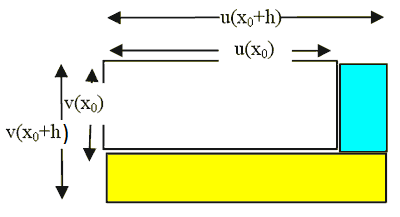
\includegraphics[width=0.5\textwidth]
{../Mathematik_1/Bilder/ableitung_produktregel_flaechenzerlegung.png}
\end{exabox}


\subsubsection*{Verkettungen}

Besonders h�ufig entstehen Funktionen dadurch, dass das Ergebnis einer
Funktion als Argument einer weiteren Funktion verwendet wird:
\[
x\longmapsto g(x)\longmapsto f(g(x)).
\]

Eine kleine �nderung von \(x\) ver�ndert zun�chst den Wert von \(g\).
Diese �nderung wird anschlie�end durch \(f\) weiterverarbeitet. Die
gesamte lokale �nderungsrate entsteht deshalb aus beiden lokalen
�nderungsraten.

\begin{theorembox}{Kettenregel}{ }
Ist \(g\) in \(x\) und \(f\) in \(g(x)\) differenzierbar, so gilt
\[
(f\circ g)'(x)
=
f'(g(x))\,g'(x).
\]
Kurz:
\[
(f\circ g)'=(f'\circ g)\,g'.
\]
\end{theorembox}

Die Kettenregel ist besonders wichtig, weil viele in Anwendungen
auftretende Funktionen Verkettungen elementarer Funktionen sind.

\begin{exabox}{Kettenregel}{ }
F�r
\[
F(x)=e^{-2x}
\]
besteht die Funktion aus der �u�eren Funktion
\[
f(u)=e^u
\]
und der inneren Funktion
\[
g(x)=-2x.
\]
Damit folgt
\[
F'(x)
=
e^{-2x}\cdot(-2)
=
-2e^{-2x}.
\]
\end{exabox}


\subsubsection*{Quotienten}

Ein Quotient kann als Produkt mit dem Kehrwert aufgefasst werden. Aus
Produkt- und Kettenregel ergibt sich dadurch die Quotientenregel.

\begin{theorembox}{Quotientenregel}{ }
Sind \(f\) und \(g\) differenzierbar und gilt \(g(x)\neq0\), so ist
\[
\left(\frac fg\right)'(x)
=
\frac{f'(x)g(x)-f(x)g'(x)}
     {(g(x))^2}.
\]
\end{theorembox}


\subsection{Standardableitungen}

Die Ableitungsregeln beschreiben, wie sich bereits bekannte Ableitungen
kombinieren lassen. Zus�tzlich werden daher die Ableitungen einiger
elementarer Funktionen ben�tigt.

Die folgende �bersicht bildet zusammen mit den Ableitungsregeln den
grundlegenden Werkzeugkasten f�r die folgenden Rechnungen.

\begin{theorembox}{Standardableitungen}{ }
\[
\begin{array}{rcl}
(C)' &=& 0,\\[0.5ex]
(x^n)' &=& nx^{n-1},
\qquad n\in\mathbb N,\\[0.5ex]
(e^x)' &=& e^x,\\[0.5ex]
(b^x)' &=& \ln(b)b^x,
\qquad b>0,\\[0.5ex]
(\ln x)' &=& \displaystyle\frac1x,
\qquad x>0,\\[1ex]
(\sin x)' &=& \cos x,\\
(\cos x)' &=& -\sin x,\\
(\tan x)' &=& \displaystyle\frac1{\cos^2x},\\[1ex]
(\arcsin x)' &=&
\displaystyle\frac1{\sqrt{1-x^2}},
\qquad -1<x<1,\\
(\arccos x)' &=&
-\displaystyle\frac1{\sqrt{1-x^2}},
\qquad -1<x<1,\\
(\arctan x)' &=&
\displaystyle\frac1{1+x^2}.
\end{array}
\]
\end{theorembox}

Die Herleitungen ausgew�hlter Standardableitungen stehen im
\textbf{(+)-Teil}. Dort wird insbesondere sichtbar, wie die bekannten
Eigenschaften von Exponential-, Logarithmus- und trigonometrischen
Funktionen mit ihren Ableitungen zusammenh�ngen.


\subsection{Zusammengesetzte Funktionen systematisch ableiten}

Bei komplizierteren Funktionstermen besteht die eigentliche Aufgabe h�ufig
nicht in der Durchf�hrung einer einzelnen Ableitungsregel, sondern im
Erkennen der Struktur des Terms.

Beispielsweise besitzt
\[
	F(x)=3\cdot e^{-(2\cdot x+1)^2}
\]
vier Ebenen:

\[
x
\longmapsto
2\cdot x + 1
\longmapsto
-(2\cdot x + 1)^2
\longmapsto
e^{-(2\cdot x + 1)^2}
\longmapsto
3 \cdot e^{-(2\cdot x + 1)^2} .
\]

Die Ableitung wird entsprechend von au�en nach innen aufgebaut. 

\begin{exabox}{Zusammengesetzte Funktion}{ }
F�r
\[
	F(x)=3\cdot e^{-(2\cdot x+1)^2}
\]
gilt
\[
F'(x)
=
3\cdot e^{-(2\cdot x+1)^2}\cdot(-2\cdot (2\cdot x+1))\cdot 2
=
- 12 \cdot (2\cdot x+1) \cdot e^{-(2\cdot x+1)^2}.
\]
\end{exabox}

Bei st�rker verschachtelten Termen wird dieses Prinzip wiederholt. Die
�u�ere Struktur entscheidet �ber die zuerst anzuwendende Regel; innere
Funktionen werden anschlie�end auf dieselbe Weise weiter zerlegt.

\subsection{Exponentialfunktionen und proportionale �nderung}
\label{MA1-ableitungsregeln-exponentialfunktion}

Die Exponentialfunktion besitzt eine f�r viele Anwendungen besonders
wichtige Eigenschaft: Ihre Ableitung ist wieder eine Exponentialfunktion.

F�r \(a>0\) gilt
\[
\frac{\mathrm d}{\mathrm dx}a^x
=
\ln(a)\,a^x.
\]

Die Ableitung ist also proportional zum Funktionswert. F�r
\(f(x)=a^x\) gilt
\[
f'(x)=\ln(a)\,f(x).
\]

Damit l�sst sich eine einfache Faustregel formulieren:

\medskip
\noindent
\textbf{Faustregel:}
Immer wenn die momentane �nderungsrate einer Gr��e proportional zu ihrem
aktuellen Wert ist, ist eine Exponentialfunktion zu erwarten.
\medskip

Ein typisches Modell hat daher die Form
\[
y'(t)=\lambda y(t).
\]
Dabei beschreibt \(y(t)\) den aktuellen Wert der betrachteten Gr��e und
\(y'(t)\) ihre momentane �nderungsrate. Der Faktor \(\lambda\) gibt an,
wie gro� die �nderungsrate im Verh�ltnis zum aktuellen Wert ist.

Ein typisches Modell hat daher die Form
\[
y'(t)=\lambda y(t).
\]
Dabei beschreibt \(y(t)\) den aktuellen Wert der betrachteten Gr��e und
\(y'(t)\) ihre momentane �nderungsrate. Der Faktor \(\lambda\) gibt an,
wie gro� die �nderungsrate im Verh�ltnis zum aktuellen Wert ist.

Die L�sungen dieser Gleichung sind genau die Funktionen
\[
y(t)=Ce^{\lambda t},
\qquad C\in\mathbb R.
\]
Tats�chlich gilt
\[
y'(t)
=
\lambda Ce^{\lambda t}
=
\lambda y(t).
\]

F�r \(\lambda>0\) w�chst die Gr��e, f�r \(\lambda<0\) nimmt sie ab.
Je gr��er dabei der aktuelle Betrag von \(y(t)\) ist, desto gr��er ist
auch der Betrag ihrer momentanen �nderung.


\begin{exabox}{Proportionales Wachstum}{}
Eine Gr��e \(y(t)\) erf�lle
\[
y'(t)=y(t),
\qquad
y(0)=y_0.
\]
Die �nderungsrate ist hier zu jedem Zeitpunkt gleich dem aktuellen Wert.
Die Funktion
\[
y(t)=y_0e^t
\]
besitzt genau diese Eigenschaft, denn
\[
y'(t)=y_0e^t=y(t)
\]
und \(y(0)=y_0\).
\end{exabox}

\subsubsection*{Die nat�rliche Exponentialfunktion}

F�r die nat�rliche Exponentialfunktion ist der Proportionalit�tsfaktor
gleich eins:
\[
\left(e^x\right)'=e^x.
\]

Funktionswert und momentane �nderungsrate stimmen daher bei \(e^x\)
�berein. Diese Eigenschaft erkl�rt, weshalb die nat�rliche
Exponentialfunktion bei der Beschreibung von Wachstums- und
Zerfallsprozessen eine besondere Rolle spielt.


\noindent\textbf{Ausblick (+):}
Die Verbindung zwischen Exponentialfunktionen und �nderungsprozessen wird
sp�ter bei Differentialgleichungen wieder aufgegriffen. Eine komplexe
Exponentialfunktion der Form
\[
e^{(\sigma+i\omega)t}
=
e^{\sigma t}\,e^{i\omega t}
\]
verbindet dabei zwei grundlegende Verhaltensweisen: Der reelle Faktor
\(e^{\sigma t}\) beschreibt Wachstum oder D�mpfung. Wegen
\[
e^{i\omega t}
=
\cos(\omega t)+i\sin(\omega t)
\]
beschreibt der zweite Faktor eine Schwingung.

\subsection{Herleitungen und Beweisideen (+)}

Die bisher zusammengestellten Regeln reichen aus, um Ableitungen
praktisch zu berechnen. Ihre Herleitungen zeigen zus�tzlich, weshalb
diese Regeln gelten und wie sie mit der Definition der Ableitung und der
lokalen Linearisierung zusammenh�ngen.

Dieser Teil ist f�r die Anwendung der Regeln nicht erforderlich, macht
aber die gemeinsame mathematische Struktur sichtbar.


\subsubsection*{Herleitung der Produktregel}

Sind \(f\) und \(g\) in \(x\) differenzierbar, so besitzen beide eine
lokale Linearisierung:
\[
f(x+h)
=
f(x)+f'(x)h+o(h)
\]
und
\[
g(x+h)
=
g(x)+g'(x)h+o(h).
\]

F�r das Produkt ergibt sich damit
\begin{eqnarray*}
f(x+h)g(x+h)
&=&
\left(f(x)+f'(x)h+o(h)\right)
\left(g(x)+g'(x)h+o(h)\right)\\[1ex]
&=&
f(x)g(x)
+
\left(f'(x)g(x)+f(x)g'(x)\right)h
+
o(h).
\end{eqnarray*}

Der lineare Anteil der �nderung besitzt somit den Koeffizienten
\[
f'(x)g(x)+f(x)g'(x).
\]
Nach der Charakterisierung der Differenzierbarkeit durch lokale
Linearisierung ist genau dieser Koeffizient die Ableitung des Produkts.

\begin{theorembox}{Produktregel}{ }
\[
(fg)'
=
f'g+fg'.
\]
\end{theorembox}


\subsubsection*{Herleitung der Kettenregel}

Nun wird die Verkettung
\[
x\mapsto f(g(x))
\]
betrachtet. Die Funktion \(g\) sei in \(x\) differenzierbar und \(f\) in
\(g(x)\).

F�r die innere Funktion gilt
\[
g(x+h)
=
g(x)+g'(x)h+o(h).
\]
Die �nderung des Arguments der �u�eren Funktion ist daher
\[
h_2
:=
g(x+h)-g(x)
=
g'(x)h+o(h).
\]

Da auch \(f\) differenzierbar ist, gilt
\[
f(g(x)+h_2)
=
f(g(x))+f'(g(x))h_2+o(h_2).
\]

Einsetzen von \(h_2\) liefert
\[
f(g(x+h))
=
f(g(x))
+
f'(g(x))g'(x)h
+
o(h).
\]

Der lineare Koeffizient ist somit
\[
f'(g(x))g'(x).
\]

\begin{theorembox}{Kettenregel}{ }
\[
(f\circ g)'(x)
=
f'(g(x))g'(x).
\]
\end{theorembox}

Die Kettenregel macht damit mathematisch pr�zise, was bereits bei ihrer
Einf�hrung anschaulich sichtbar war: Eine kleine �nderung von \(x\) wird
zun�chst durch \(g\) und anschlie�end durch \(f\) weitergegeben. Die
beiden lokalen �nderungsfaktoren multiplizieren sich.


\subsubsection*{Herleitung der Quotientenregel}

Zun�chst wird die Ableitung der Kehrwertfunktion betrachtet. Aus
\[
x\cdot\frac1x=1
\]
folgt mit der Produktregel
\[
0
=
\left(x\cdot\frac1x\right)'
=
\frac1x
+
x\left(\frac1x\right)'.
\]
Damit gilt
\[
\left(\frac1x\right)'
=
-\frac1{x^2}.
\]

F�r eine differenzierbare Funktion \(g\) folgt mit der Kettenregel
\[
\left(\frac1{g(x)}\right)'
=
-\frac{g'(x)}{(g(x))^2}.
\]

Schlie�lich wird
\[
\frac{f(x)}{g(x)}
=
f(x)\frac1{g(x)}
\]
als Produkt aufgefasst. Die Produktregel ergibt
\[
\left(\frac fg\right)'
=
\frac{f'g-fg'}{g^2}.
\]


\subsubsection*{Herleitungen ausgew�hlter Standardableitungen}

\paragraph{Exponentialfunktion.}

Aus dem \underline{bekannten Grenzwert}\randverweis{MA1-grenzwerte-von-folgen-und-funktionen}
\[
\lim_{h\to0}\frac{e^h-1}{h}=1
\]
folgt unmittelbar
\begin{eqnarray*}
\frac{e^{x+h}-e^x}{h}
&=&
e^x\frac{e^h-1}{h}.
\end{eqnarray*}
Damit ergibt sich f�r \(h\to0\)
\[
(e^x)'=e^x.
\]
Damit ergibt sich f�r \(h\to0\)
\[
(e^x)'=e^x.
\]

\begin{theorembox}{Ableitung der Exponentialfunktion}{ }
\[
\exp'=\exp.
\]
\end{theorembox}

F�r eine beliebige Basis \(b>0\) gilt
\[
b^x=e^{x\ln b}.
\]
Mit der Kettenregel folgt
\[
(b^x)'
=
e^{x\ln b}\ln b
=
\ln(b)b^x.
\]


\paragraph{Logarithmusfunktion.}

Exponentialfunktion und nat�rlicher Logarithmus sind Umkehrfunktionen.
F�r \(x>0\) gilt
\[
e^{\ln x}=x.
\]
Ableiten beider Seiten und Anwenden der Kettenregel liefert
\[
e^{\ln x}(\ln x)'=1.
\]
Wegen \(e^{\ln x}=x\) folgt
\[
(\ln x)'=\frac1x.
\]


\paragraph{Potenzfunktionen.}

F�r \(x>0\) l�sst sich
\[
x^n=e^{n\ln x}
\]
schreiben. Mit der Kettenregel folgt
\begin{eqnarray*}
\frac{\mathrm d}{\mathrm dx}x^n
&=&
\frac{\mathrm d}{\mathrm dx}e^{n\ln x}\\
&=&
e^{n\ln x}\frac{n}{x}\\
&=&
nx^{n-1}.
\end{eqnarray*}

F�r \(n\in\mathbb N\) gilt diese Ableitungsregel auf dem gesamten
Definitionsbereich der jeweiligen Potenzfunktion.


\paragraph{Trigonometrische Funktionen.}

Eine besonders kompakte Herleitung ergibt sich mithilfe der Eulerschen
Identit�t
\[
e^{ix}=\cos x+i\sin x.
\]
Ableiten liefert
\[
\frac{\mathrm d}{\mathrm dx}e^{ix}
=
ie^{ix}
=
i(\cos x+i\sin x)
=
-\sin x+i\cos x.
\]

Durch Vergleich von Real- und Imagin�rteil folgt
\[
(\cos x)'=-\sin x,
\qquad
(\sin x)'=\cos x.
\]

F�r den Tangens ergibt sich anschlie�end mit der Quotientenregel
\begin{eqnarray*}
(\tan x)'
&=&
\left(\frac{\sin x}{\cos x}\right)'\\
&=&
\frac{\cos^2x+\sin^2x}{\cos^2x}\\
&=&
\frac1{\cos^2x}.
\end{eqnarray*}


\paragraph{Inverse trigonometrische Funktionen.}

Die Ableitungen der inversen trigonometrischen Funktionen lassen sich
�hnlich wie die Ableitung des Logarithmus aus der Beziehung zwischen
einer Funktion und ihrer Umkehrfunktion gewinnen.

F�r den Arkussinus gilt
\[
\sin(\arcsin x)=x.
\]
Ableiten liefert
\[
\cos(\arcsin x)(\arcsin x)'=1.
\]
Da
\[
\cos(\arcsin x)=\sqrt{1-x^2}
\qquad\textnormal{f�r }-1<x<1,
\]
folgt
\[
(\arcsin x)'
=
\frac1{\sqrt{1-x^2}}.
\]

Entsprechend ergeben sich
\[
(\arccos x)'
=
-\frac1{\sqrt{1-x^2}},
\qquad -1<x<1,
\]
und
\[
(\arctan x)'
=
\frac1{1+x^2}.
\]
 \newpage % Ableitungsregeln
\setcounter{exercise}{0} 
\ifintegriereaufgaben
\section*{Differentiation Aufgaben}\label{MA1-ableitungsregeln-aufgaben}

	Regeln und Beispiele, die zur Bearbeitung der Aufgaben hilfreich sind, finden Sie im Skript\wennreferenzvorhanden{MA1-ableitungsregeln}{ (Abschnitt \abschnittsverweis{MA1-ableitungsregeln})} und, falls Sie nicht weiterkommen, schauen Sie \hyperref[MA1-ableitungsregeln-loesungen]{hier}.
\else
\section{Differentiation Aufgaben}\label{MA1-ableitungsregeln-aufgaben}

	Regeln und Beispiele, die zur Bearbeitung der Aufgaben hilfreich sind, finden Sie im Skript und, falls Sie nicht weiterkommen, schauen Sie \hyperref[MA1-ableitungsregeln-loesungen]{hier}.
\fi 

\begin{exercisebox}[Differenzierbarkeit]
  \begin{itemize}
	  \item[(a)] Untersuchen Sie, ob $f$ an der Stelle  $x_0 = 1$ differenzierbar ist:
		  \[ f:\mathbb R \to \mathbb R, x\mapsto  
			  \begin{cases} 1-x^2, \; x \leq 1\,, \\
    x^2 -1, \; x > 1\,.\end{cases} 
      \]
      \item[(b)] Bestimmen Sie die Parameter $a,b\in\mathbb R$ so, dass $g$ auf ganz $\mathbb R$ differenzierbar ist: 
		  \[ g:\mathbb R \to \mathbb R, x\mapsto  
			  \begin{cases} a\cdot x^2, \; x \geq 1\,, \\
    x +b, \; x < 1\,.\end{cases} 
      \]
    %\item $ f(x) = x\cdot |x|, \; x_0 = 0  $
    %\item $ f(x) = |x| \cdot (x-3), \; x_0 = 3  $
  \end{itemize}
\end{exercisebox} 

\begin{exercisebox}[Differenzierbarkeit]
	Bestimmen Sie die Ableitung der Funktion $f:x\mapsto \sqrt{x}$ mit Hilfe des Differenzenquotienten.
\end{exercisebox}

\begin{exercisebox}[Bedeutung der Ableitung]
	Skizzieren Sie die Ableitung f�r Funktion.
	\begin{center}
	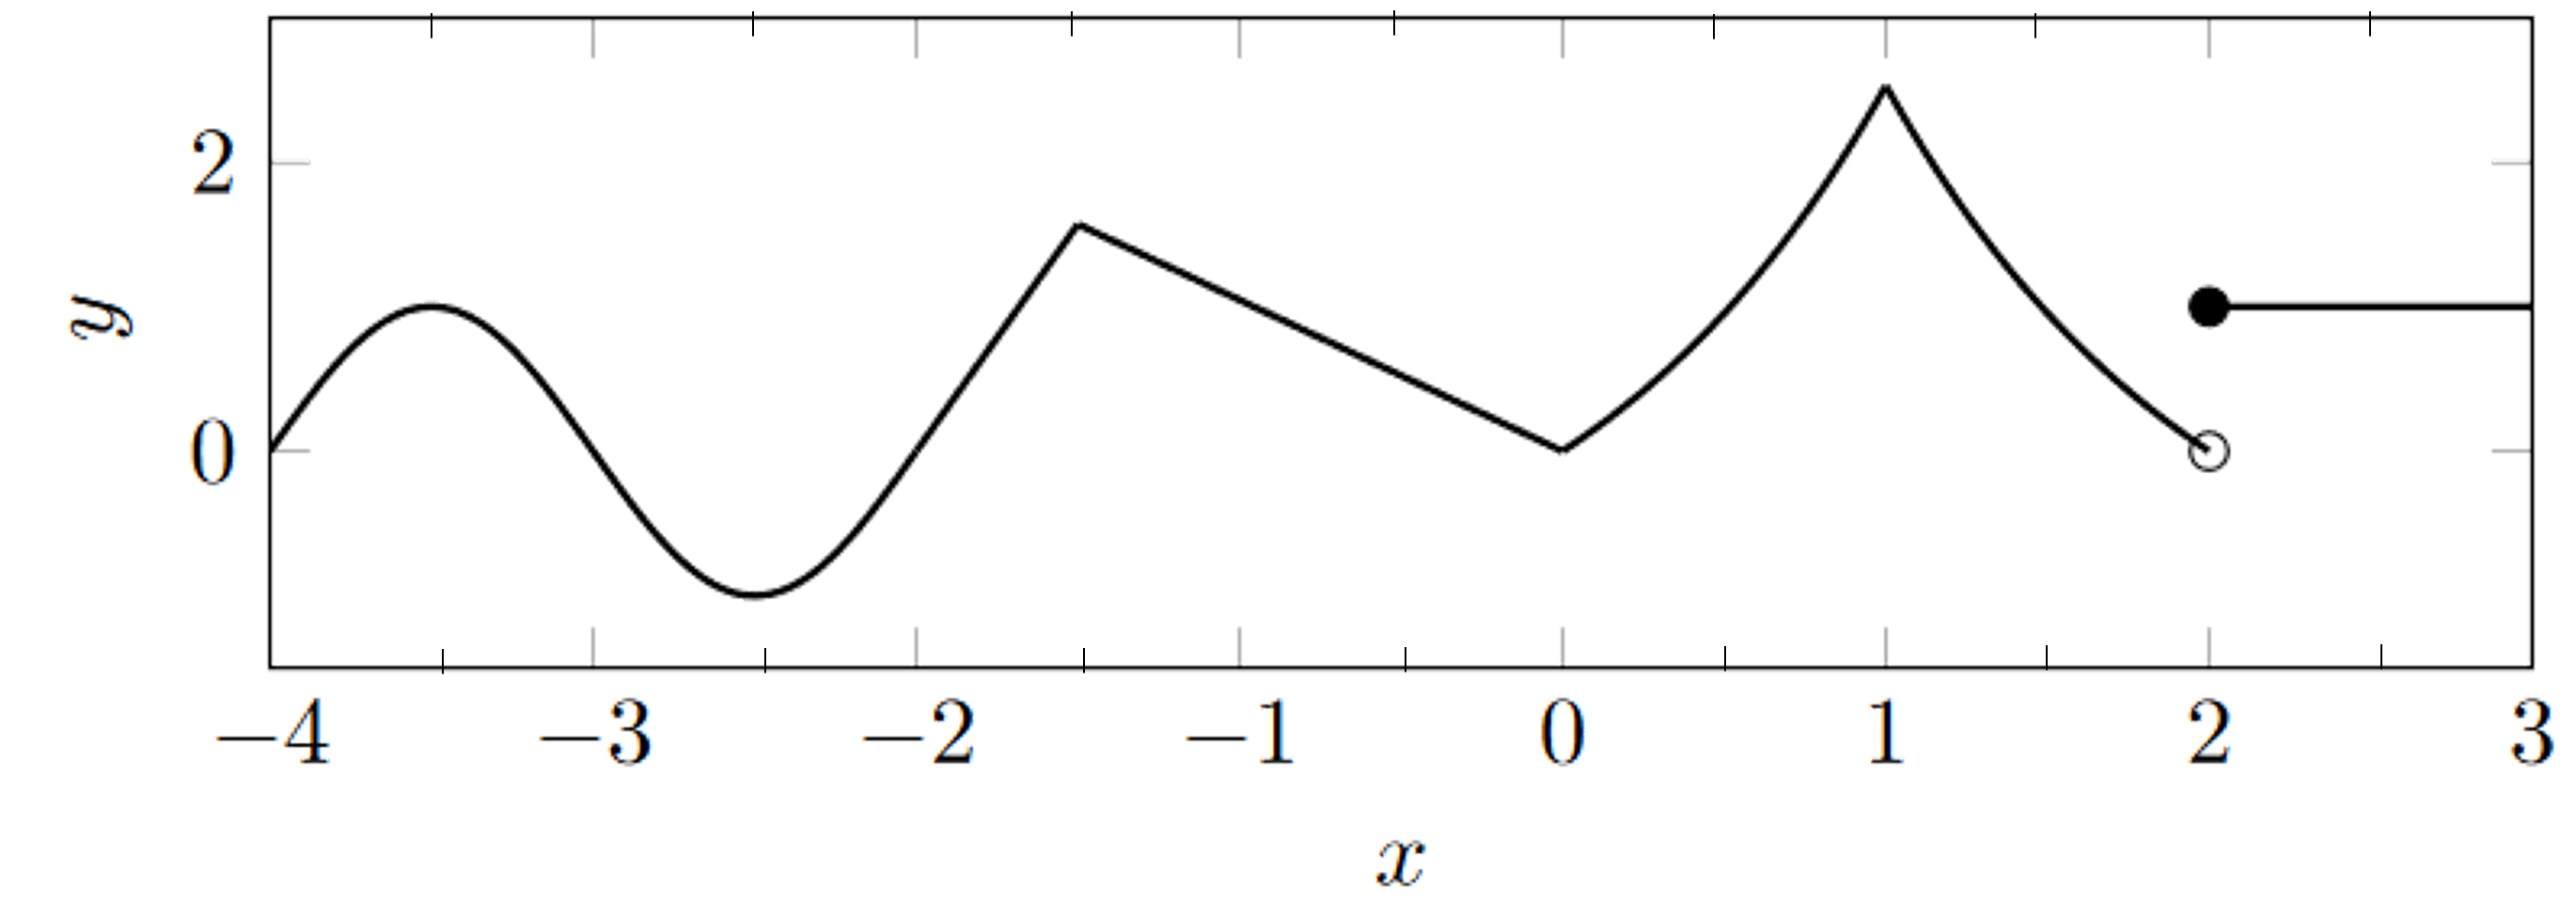
\includegraphics[width=0.75\textwidth]{../Mathematik_1/Bilder/ableitung_graphisch_skizzieren_aufgabe.png}
\end{center}
\end{exercisebox} 

\begin{exercisebox}[Differenzieren]
	Berechnen Sie von den folgenden Funktionen die Ableitungen. Es ist $a\in \mathbb R$ ein Parameter.
	\begin{eqnarray*}
		\begin{array}{ll}
			(a)\; f(x) = \mathrm{cosh}(x) = \displaystyle{\frac{e^x + e^{-x}}{2}} &\quad (b)\; g(u) = \displaystyle{\frac{u^2}{u^2+a^2}} \\[2ex]
			(c)\; h(p) = \mathrm{exp}\left(-p^2/(2a)^2\right) &\quad (d)\; i(x) = \displaystyle{\frac{(2x+3)^2-2}{\sqrt{x-1}}} \\
		\end{array}
	\end{eqnarray*}
\end{exercisebox}

\begin{exercisebox}[Anwendung: Monotonie-Satz]
Angenommen Sie wissen �ber eine Funktion $f$, dass ihre Ableitung auf einem Intervall $I$ negativ ist, also $f'(x) \leq 0$. Was k�nnen Sie dann �ber das Monotonie-Verhalten aussagen?
\end{exercisebox}

\begin{exercisebox}[Anwendungen: Lineare N�herung]
	Die Mittellinie einer Rennstrecke der Breite $2\, \mathrm{m}$ wird durch Funktion $x\mapsto 4-\frac12 x^2$ beschrieben. Wir beobachten einen Rennwagen der die Bahnkurve im Uhrzeigersinn entlang rast. Bei spiegelglatter Fahrbahn rutscht das Fahrzeug und landet im Punkt $Y(0|6)$ in den Strohballen. Wo hat das Fahrzeug die Stra�e verlassen? 
\end{exercisebox} 


%
%%\begin{exercisebox}[Differenzierbarkeit]
%%  Untersuchen Sie, ob $f$ an der Stelle $x_0$ differenzierbar ist.
%%  \begin{enumerate}
%%    \item $f(x) = \begin{cases} x^2-2x, x<3\\ \frac16x^3-\frac12x, x\geq 3\end{cases}, x_0 = 3$
%%    \item $f(x) = \begin{cases} \frac{x-2}{x}, x>2\\ 2-x, x\leq 2\end{cases}, x_0 = 2$
%%    \item $f(x) = |x-2|, \; x_0 = 2$
%%    \item $f(x) = (x-1)\cdot |x-1|, \; x_0 = 1$
%%    \item $f(x) = \sqrt{(x^2-1)^2}, \; x_0 = 1$
%%    \item $f(x) = \frac{x}{|x|+1}, \; x_0 = 0$
%%  \end{enumerate}
%%\end{exercisebox}
%
%\begin{exercisebox}[Kettenregel]
%  Leiten Sie ab und vereinfachen Sie das Ergebnis soweit wie m�glich:
%  \begin{eqnarray*}
%	  \begin{array}{lll}  
%		  (a)\; g(x) = \left( f(x) \right)^n, \quad n \in \mathbb N
%    &\quad (b)\; f(x) = \frac{1}{18}(3x+2)^6
%    &\quad (c)\; f(x) = 2(5-x)^{-1}\\
%    (d)\; f(r) = \sqrt{7r-r^2}
%    &\quad (e)\; f(x) = (1+\sqrt{x})^2
%    &\quad (f)\; f(x) = \frac{1}{x^2}+\sin(\frac{1}{x})
%    %&\quad (a) f(x) = \sin\left( (ax)^2 \right)$
%    %\item $f(x) = \frac{1}{(x-2)^2}$
%    %\item $f(x) = (x+x^2)^2$
%    %\item $f(t) = \frac{5}{(t^2-1)^2}$
%    %\item $f(x) = \frac{1}{a+bx}$
%  \end{array}
%  \end{eqnarray*}
%\end{exercisebox} 
%
%\begin{exercisebox}[Prduktregel]
%  Leiten Sie ab und vereinfachen Sie das Ergebnis soweit wie m�glich:
%  \begin{eqnarray*}
%	  \begin{array}{lll}  
%		  (a)\; f(x) = x\sqrt{x} 
%	    & \quad (b) \; g(t) = (2t^2-3)\sqrt{t} 
%     & \quad (c) \; f(x) = x\cdot \sin(x) \\
%     (d) \; f(x) = (kx+1)\cdot \sin(x) 
%     & \quad (e) \; f(x) = (x^2+1)\cdot \cos(x)
%     & \quad (f) \; f(x) = (2x+3)^3(2x-1)^2
%     %& \quad (g) \; f(x) = \sqrt{x}(x-t)$
%     %& \quad (h) \; f(x) = x^2\sqrt{x}$
%     %& \quad (i) \; f(x) = \sin(2x)\cdot \cos(2x)$
%     %& \quad (j) \; f(a) = \sqrt{a}(1-2a^3)$
%  \end{array}
%  \end{eqnarray*}
%\end{exercisebox} 
%
%\begin{exercisebox}[Quotientenregel]
%  Leiten Sie ab und vereinfachen Sie das Ergebnis soweit wie m�glich:
%  \begin{eqnarray*}
%	  \begin{array}{lll}  
%	(a)\; g(t) = \frac{2-t^3}{2+t^3}  
%    &\quad (b)\; h(r) = \frac{2r^4}{r^2-1}  
%    &\quad (c)\; s(t) = \frac{4t^2-5}{2t+1} \\ 
%    (d)\; z(t) = \frac{t^2-1,5t}{1+0,8t}  
%    &\quad (e)\; f(x) = \frac{\sqrt{x}+1}{\sqrt{x}-1}  
%    &\quad (f)\; f(x) = \frac{\sin(x)}{\cos(x)} \\ 
%    %&\quad (g)\; f(a) = \frac{3a}{1+x^2} $ 
%  \end{array}
%  \end{eqnarray*}
%\end{exercisebox} 
%
%\begin{exercisebox}[Ableitungen]
%  Bestimmen Sie die ersten drei Ableitungen
%  \begin{eqnarray*}
%	  \begin{array}{lll}  
%		  (a)\; f(x) = \frac34 x^4 - \frac54 x^2 + 2x  & \quad 
%		  (b)\; f(x) = (2sx^2-3tx)^2 & \quad 
%	 	  (c)\; f(x) = \frac{a^2x^2+2ax-a}{4ax} \\
%		  (d)\; f(s) = \frac{4rs^4+8r^4s^2}{2r^2s^3} & \quad 
%		  (e)\; f(x) = -2a\sin(\frac34 ax) & \quad 
%		  (f)\; f(x) = \frac{2}{t}\cos(-2tx) 
%	%\item $ f(x) = 0,5x^3+3x^2-4  $
%	%\item $ f(x) = 2\left( \frac15 x^7 + \frac35 x^6\right)$
%	%\item $ f(x) = ax^3 + bx^2 +cx + d$
%	%\item $ f(x) = 2r^2x^4-4rx^3+r$
%	%\item $ f(s) = \frac{a^2x^2+2ax-a}{4ax} + s$
%	  \end{array}
%  \end{eqnarray*}
%\end{exercisebox} 

%\begin{exercisebox}[Ableitung]
%	Exponentialfunktionen, trigonometrische Funktionen - mittels Potenzreihen ? 
%\end{exercisebox} 
%
%\begin{exercisebox}[Reihendarstellung von $\exp$ aus Ableitungseigenschaft]
%	$\exp' = \exp$ Entwicklung der Reihe. Zeige zuerst dass an der Stelle $x=0$ Tangente mit Steigung $m=1$.
%\end{exercisebox} 

%\begin{exercisebox}[Differenzierbarkeit verlangt Stetigkeit]
%  Ist die Stetigkeit eine notwendige oder hinreichende Bedingung f�r Differenzierbarkeit?
%\end{exercisebox}

%\begin{exercisebox}[Ableitung von Area-Funktionen, mit Hinweis]
%\end{exercisebox}

%\begin{exercisebox}[Umkehrfunktion, strenge Montonie, strenge Montonie]
%\end{exercisebox}
%
%\begin{exercisebox}[Zwischenwertsatz, Mittelwertsatz]
%\end{exercisebox}

%\begin{theorembox}[Merkregel: Kettenregel]
%  �u�ere Ableitung mal innere Ableitung.
%\end{theorembox}

 \newpage 
\setcounter{satz}{0} \setcounter{def}{0} \setcounter{exa}{0}  \section{Lokale Linearit�t}\label{MA1-lokale-linearitaet}

\begin{table}[H]
  \centering
  \begin{tabularx}{\textwidth}{p{0.9\textwidth} p{0.1\textwidth}}
    \toprule
    \multicolumn{2}{c}{\textbf{�bersicht �ber Lernziele und Voraussetzungen}}\\
    \midrule
    \textbf{Lernziele} &\\[.5\normalbaselineskip]
    \tabitem Differenzierbarkeit als lokale Linearit�t interpretieren &\\
    \tabitem eine Funktion durch ihre Tangente lokal approximieren &\\
    \tabitem die Bedeutung der Kr�mmung f�r die Genauigkeit einer
             Linearisierung erkl�ren &\\
    \tabitem die Regel von L'Hospital zur Untersuchung geeigneter
             Grenzwerte anwenden &\\
    \tabitem Ableitungen aus diskreten Funktionswerten durch
             Differenzenquotienten approximieren &\\
    \tabitem das Newton-Verfahren als wiederholte Linearisierung
             erkl�ren und anwenden &\\
    \midrule
    \textbf{Voraussetzungen} &\\[.5\normalbaselineskip]
    \tabitem Grenzwerte von Funktionen verstehen & \abschnittsverweis{MA1-grenzwerte-von-folgen-und-funktionen}\\
    \tabitem Differenzierbarkeit und Ableitung interpretieren & \abschnittsverweis{MA1-stetigkeit-und-differenzierbarkeit}\\
    \tabitem Ableitungen berechnen & \abschnittsverweis{MA1-ableitungsregeln}\\
    \bottomrule
  \end{tabularx}
\end{table}

\ifintegriereaufgaben
\noindent �bungsaufgaben zum Thema:
\hyperref[MA1-lokale-linearitaet-aufgaben]{Aufgaben}
\vspace{0.3cm}
\hrule
\fi


% =========================================================
\subsection{Differenzierbarkeit bedeutet lokale Linearit�t}
\label{MA1-lokale-linearitaet-differenzierbarkeit}

Viele Funktionen, die in Anwendungen auftreten, sind nichtlinear.
Nichtlineare Funktionen und Gleichungen sind im Allgemeinen schwieriger
zu untersuchen als lineare. Die Differenzierbarkeit er�ffnet jedoch einen
grundlegenden Zugang:

\medskip
\noindent
\emph{In hinreichend kleiner Umgebung kann eine differenzierbare Funktion
durch ein lineares Modell ersetzt werden.}
\medskip

Dieses Prinzip hei�t \textbf{Linearisierung} (\emph{linearization}).
Es geh�rt zu den grundlegenden Ideen der Analysis und insbesondere der
Numerik. Statt ein nichtlineares Problem unmittelbar zu behandeln, wird
es zun�chst lokal durch ein einfacheres lineares Problem ersetzt.

Ist \(f\) in \(x_0\) differenzierbar, so ist die Tangente
\[
T_{x_0}(x)
=
f(x_0)+f'(x_0)(x-x_0)
\]
die lokale affine Approximation der Funktion.

F�r \(x=x_0+h\) ergibt sich entsprechend
\[
T_{x_0}(x_0+h)
=
f(x_0)+f'(x_0)h.
\]

Die Aussage, dass die Tangente die Funktion lokal approximiert, l�sst sich
pr�zise formulieren.

\begin{theorembox}{Lokale Linearit�t}{}
Ist \(f\) in \(x_0\) differenzierbar, so gilt
\[
f(x_0+h)
=
f(x_0)+f'(x_0)h+r(h),
\]
wobei
\[
\lim_{h\to0}\frac{r(h)}{h}=0.
\]
\end{theorembox}

Der Rest \(r(h)\) verschwindet also f�r \(h\to0\) schneller als die
Schrittweite \(h\). In diesem pr�zisen Sinn wird die Funktion in immer
kleinerer Umgebung von \(x_0\) immer besser durch ihre Tangente
beschrieben.

Mit der \textbf{Landau-Schreibweise} l�sst sich die Bedingung an den Rest
kurz als
\[
r(h)=o(h)
\]
schreiben. Damit lautet die lokale Linearisierung
\[
f(x_0+h)
=
f(x_0)+f'(x_0)h+o(h).
\]

Die Ableitung \(f'(x_0)\) ist somit nicht nur eine Tangentensteigung oder
eine lokale �nderungsrate. Sie bestimmt zugleich den linearen Anteil der
lokalen �nderung von \(f\).

Anschaulich:
\[
\text{nahe }x_0:
\qquad
f
\approx
\text{Tangente}.
\]

Diese Idee wird in Mathematik~2 durch Taylor-Polynome erweitert. Dort wird
eine Funktion nicht nur durch einen linearen, sondern durch einen
polynomiellen Ausdruck h�herer Ordnung lokal approximiert.


\begin{exabox}{Lokale Approximation eines Funktionswertes}{}

F�r
\[
f(x)=\sqrt{x}
\]
ist der Funktionswert bei \(x_0=100\) unmittelbar bekannt:
\[
f(100)=10.
\]
Au�erdem gilt
\[
f'(x)=\frac{1}{2\sqrt{x}},
\qquad
f'(100)=\frac1{20}.
\]

Die Linearisierung der Wurzelfunktion bei \(x_0=100\) lautet daher
\[
T_{100}(x)
=
10+\frac1{20}(x-100).
\]

F�r \(x=103\) ergibt sich
\[
\sqrt{103}
\approx
T_{100}(103)
=
10+\frac3{20}
=
10{,}15.
\]

Die nichtlineare Wurzelfunktion wurde damit in der N�he von \(100\) durch
eine affine Funktion ersetzt. Die eigentliche N�herungsrechnung ist
anschlie�end nur noch linear.
\end{exabox}

\noindent\textbf{Bemerkung:}
Linearisierung ist eine lokale Aussage. Je weiter sich \(x\) von der
Entwicklungsstelle \(x_0\) entfernt, desto st�rker kann sich die Funktion
von ihrer Tangente unterscheiden.


% =========================================================
\subsection{Wie gut ist die Linearisierung?}
\label{MA1-lokale-linearitaet-fehlerabschaetzung}

Eine N�herung ist besonders dann n�tzlich, wenn zumindest eingesch�tzt
werden kann, wie gro� ihr Fehler ist.

Die Tangente stimmt an der Stelle \(x_0\) mit der Funktion im Funktionswert
und in der Steigung �berein:
\[
T_{x_0}(x_0)=f(x_0),
\qquad
T_{x_0}'(x_0)=f'(x_0).
\]

Entfernt sich \(x\) von \(x_0\), macht sich jedoch die
\textbf{Kr�mmung} der Funktion bemerkbar. Eine nahezu geradlinig
verlaufende Funktion bleibt �ber einen gr��eren Bereich nahe an ihrer
Tangente; bei starker Kr�mmung verliert die Tangentenapproximation
schneller an Genauigkeit.

Die zweite Ableitung liefert ein Ma� f�r diese Kr�mmung. Damit entsteht
der qualitative Zusammenhang
\[
\text{gro�es }|f''|
\quad\Longrightarrow\quad
\text{st�rkere Abweichung von der Tangente}.
\]

Diese Beobachtung f�hrt zu einer quantitativen Fehlerabsch�tzung.


\subsubsection*{Fehlerabsch�tzung (+)}

Ist \(f\) zweimal stetig differenzierbar und gilt
\[
|f''(x)|\le M
\]
f�r alle \(x\) zwischen \(x_0\) und \(x_0+h\), so l�sst sich der Fehler
der linearen Approximation absch�tzen.

\begin{theorembox}{Fehler der linearen Approximation}{}
Unter den genannten Voraussetzungen gilt
\[
\left|
f(x_0+h)
-
\bigl(f(x_0)+f'(x_0)h\bigr)
\right|
\le
\frac{M}{2}h^2.
\]
\end{theorembox}

Der Fehler ist damit h�chstens von der Gr��enordnung \(h^2\). Wird die
Schrittweite beispielsweise halbiert, so wird dieser Anteil der
Fehlerabsch�tzung um den Faktor vier kleiner.

Die systematische Herleitung dieser Aussage erfolgt sp�ter mithilfe des
Taylor-Satzes. F�r den Moment ist vor allem die Struktur wichtig:
Die erste Ableitung liefert die lineare Approximation, die zweite
Ableitung kontrolliert deren Fehler.


\begin{exabox}{Fehlerabsch�tzung f�r \(\sqrt{103}\)}{}

F�r
\[
f(x)=\sqrt{x}
\]
gilt
\[
f''(x)
=
-\frac{1}{4x^{3/2}}.
\]

Im Intervall \([100,103]\) gilt daher
\[
|f''(x)|
\le
\frac1{4000}.
\]
Mit \(h=3\) folgt
\[
\left|
\sqrt{103}-10{,}15
\right|
\le
\frac12\cdot\frac1{4000}\cdot 3^2
=
\frac9{8000}.
\]

Da \(f''(x)<0\), ist die Wurzelfunktion in diesem Bereich nach unten
gekr�mmt und liegt unterhalb ihrer Tangente. Damit ergibt sich sogar
\[
10{,}15-\frac9{8000}
\le
\sqrt{103}
\le
10{,}15.
\]

Zum Vergleich:
\[
\sqrt{103}=10{,}148891\ldots
\]
\end{exabox}


% =========================================================
\subsection{Grenzwerte durch lokale �nderungsraten:
die Regel von L'Hospital}
\label{MA1-lokale-linearitaet-lhospital}

Die lokale Beschreibung einer Funktion durch ihre Ableitung l�sst sich
auch zur Untersuchung von Grenzwerten nutzen.

Bei einem Quotienten
\[
\frac{f(x)}{g(x)}
\]
kann es vorkommen, dass f�r \(x\to x_0\) sowohl Z�hler als auch Nenner
gegen null streben. Direktes Einsetzen f�hrt dann auf die
\textbf{unbestimmte Form}
\[
\frac00.
\]
Dieser Ausdruck besitzt keinen eigenen Zahlenwert. Er zeigt vielmehr an,
dass aus den Grenzwerten von Z�hler und Nenner allein noch nicht folgt,
wie sich ihr Quotient verh�lt.

Die Idee der Linearisierung liefert zun�chst eine anschauliche Erkl�rung.
Seien beispielsweise
\[
f(x_0)=0,
\qquad
g(x_0)=0.
\]
Dann gilt lokal
\[
f(x_0+h)
=
f'(x_0)h+o(h)
\]
und
\[
g(x_0+h)
=
g'(x_0)h+o(h).
\]

Falls \(g'(x_0)\neq0\), werden Z�hler und Nenner in erster N�herung durch
ihre linearen Anteile beschrieben. Daher verh�lt sich der Quotient f�r
kleine \(h\) wie
\[
\frac{f(x_0+h)}{g(x_0+h)}
\approx
\frac{f'(x_0)h}{g'(x_0)h}
=
\frac{f'(x_0)}{g'(x_0)}.
\]

Die lokalen �nderungsraten k�nnen also dar�ber entscheiden, wie sich der
Quotient zweier gegen null strebender Funktionen verh�lt.

Diese �berlegung erkl�rt einen wichtigen Spezialfall der
\textbf{Regel von L'Hospital} (\emph{L'Hospital's rule}). Der allgemeine
Satz ist weiterreichend und ben�tigt eigene Voraussetzungen.


\begin{theorembox}{Regel von L'Hospital}{}
Es seien \(f\) und \(g\) in einer punktierten Umgebung von \(x_0\)
differenzierbar und es gelte dort \(g'(x)\neq0\). Weiter sei
\[
\lim_{x\to x_0}f(x)
=
\lim_{x\to x_0}g(x)
=
0.
\]

Existiert der Grenzwert
\[
\lim_{x\to x_0}
\frac{f'(x)}{g'(x)}
=
L
\]
als endlicher oder uneigentlicher Grenzwert, so gilt unter diesen
Voraussetzungen
\[
\lim_{x\to x_0}
\frac{f(x)}{g(x)}
=
L.
\]
\end{theorembox}

Eine entsprechende Aussage gilt unter geeigneten Voraussetzungen auch
f�r Quotienten der unbestimmten Form
\[
\frac{\infty}{\infty}.
\]


\begin{exabox}{Regel von L'Hospital}{}

Der Grenzwert
\[
\lim_{x\to0}
\frac{\sin x}{e^x-1}
\]
f�hrt beim direkten Einsetzen auf die unbestimmte Form \(0/0\).

Mit der Regel von L'Hospital folgt
\[
\lim_{x\to0}
\frac{\sin x}{e^x-1}
=
\lim_{x\to0}
\frac{\cos x}{e^x}
=
1.
\]

Die lokale Linearisierung macht das Ergebnis zus�tzlich anschaulich:
F�r kleine \(x\) gilt
\[
\sin x\approx x
\qquad\text{und}\qquad
e^x-1\approx x.
\]
Z�hler und Nenner besitzen bei \(x=0\) also denselben linearen Anteil.
Ihr Quotient n�hert sich deshalb dem Wert \(1\).
\end{exabox}

\noindent\textbf{Bemerkung:}
Die Linearisierung erkl�rt die Grundidee von L'Hospital besonders
anschaulich, wenn die ersten Ableitungen bereits das lokale Verhalten
bestimmen. Der allgemeine Satz ist jedoch nicht lediglich eine
Umformulierung der Tangentenapproximation.


% =========================================================
\subsection{Linearisierung aus diskreten Daten}
\label{MA1-lokale-linearitaet-diskrete-daten}

Bisher wurde die Ableitung als bekannt vorausgesetzt und daraus die
Linearisierung einer Funktion bestimmt. In Messungen, Experimenten und
numerischen Berechnungen tritt h�ufig die umgekehrte Situation auf:

Die Funktionswerte sind bekannt, die Ableitung jedoch nicht.

Beispielsweise kann eine physikalische Gr��e nur zu diskreten Zeitpunkten
gemessen worden sein. Zwischen den Messpunkten liegen dann keine
unmittelbaren Informationen �ber den Funktionsverlauf vor.

Die lokale Linearit�t liefert auch hier die entscheidende Idee. Ist eine
Funktion in einem kleinen Bereich ann�hernd geradlinig, so l�sst sich die
unbekannte Tangentensteigung durch die Steigung einer nahe gelegenen
Sekante approximieren.

F�r zwei benachbarte Funktionswerte ergibt sich beispielsweise
\[
f'(x)
\approx
\frac{f(x+h)-f(x)}{h}.
\]

Damit wird die Ableitung selbst zu einer Gr��e, die numerisch aus
Funktionswerten approximiert werden kann.


\begin{exabox}{Differenzenquotienten}{}
\begin{center}
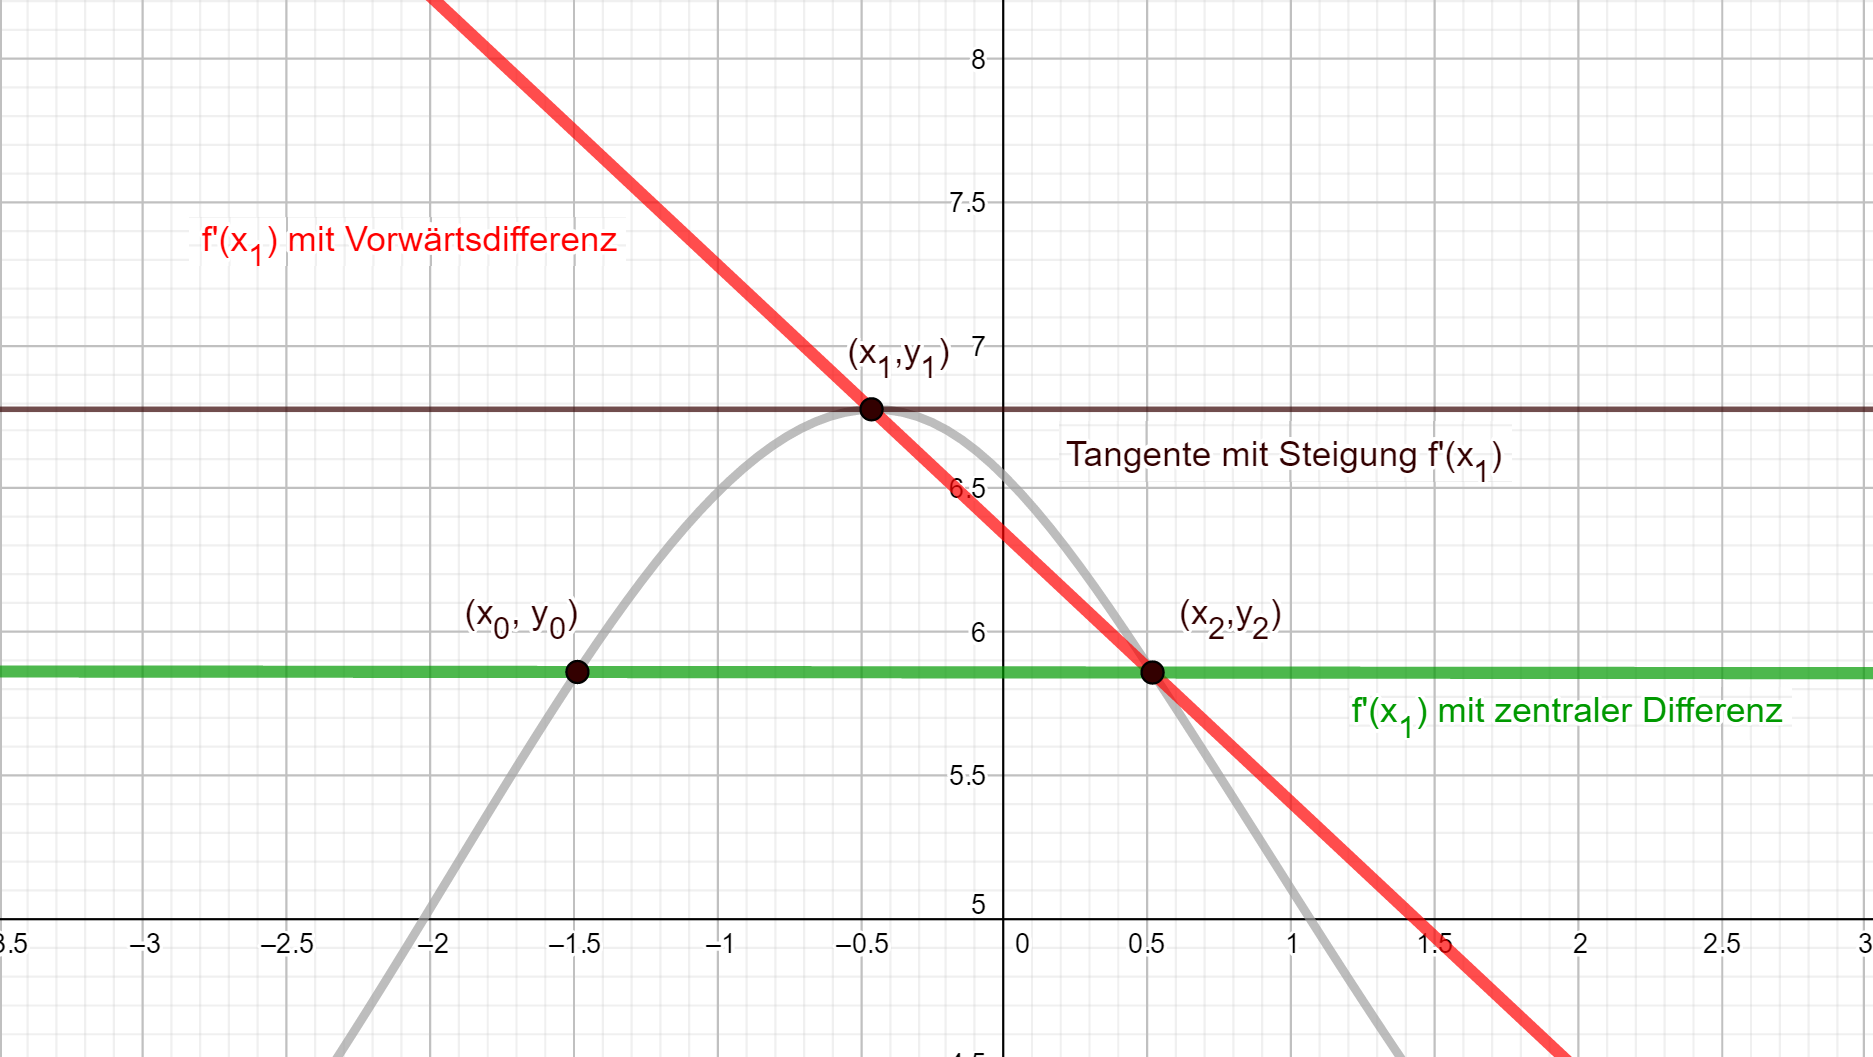
\includegraphics[width=0.8\textwidth]
{../Mathematik_1/Bilder/ableitung_differenzenquotienten_vergleich.png}
\end{center}
\end{exabox}

Werden Funktionswerte auf beiden Seiten der betrachteten Stelle verwendet,
so ergibt sich die \textbf{zentrale Differenz}
(\emph{central difference})
\[
f'(x)
\approx
\frac{f(x+h)-f(x-h)}{2h}.
\]

Geometrisch entspricht dieser Ausdruck wieder einer Sekantensteigung.
Durch die symmetrische Wahl der beiden Punkte heben sich jedoch bestimmte
Fehleranteile gegenseitig auf. Deshalb ist die zentrale Differenz bei
glatten Funktionen typischerweise genauer als die einseitige
Vorw�rtsdifferenz.


\subsubsection*{Genauigkeit von Differenzenquotienten (+)}

F�r hinreichend glatte Funktionen gelten die Fehlerordnungen
\[
\textnormal{Vorw�rtsdifferenz:}
\qquad
f'(x)
=
\frac{f(x+h)-f(x)}{h}
+
\mathcal O(h),
\]
w�hrend f�r die zentrale Differenz
\[
\textnormal{zentrale Differenz:}
\qquad
f'(x)
=
\frac{f(x+h)-f(x-h)}{2h}
+
\mathcal O(h^2)
\]
gilt.

Die zentrale Differenz besitzt damit einen Fehler zweiter Ordnung:
Wird \(h\) halbiert, verkleinert sich dieser Fehleranteil n�herungsweise
um den Faktor vier.

Auch die zweite Ableitung kann aus benachbarten Funktionswerten
approximiert werden:

\begin{theorembox}{Zweite Differenz}{}
F�r hinreichend glatte Funktionen gilt
\[
f''(x)
=
\frac{f(x+h)-2f(x)+f(x-h)}{h^2}
+
\mathcal O(h^2).
\]
\end{theorembox}

Diese Formeln sind erste Beispiele f�r ein grundlegendes Vorgehen der
Numerik: Aus endlich vielen diskreten Daten werden lokale Eigenschaften
einer kontinuierlichen Funktion approximiert.

\noindent\textbf{Bemerkung:}
Mathematisch wird die Approximation f�r kleiner werdendes \(h\) zun�chst
genauer. In tats�chlichen numerischen Rechnungen kann \(h\) jedoch nicht
beliebig klein gew�hlt werden, da Rundungsfehler und Messfehler dann
zunehmend ins Gewicht fallen. Die Wahl einer geeigneten Schrittweite ist
daher selbst Teil eines numerischen Verfahrens.


% =========================================================
\subsection{Newton-Verfahren: wiederholte Linearisierung}
\label{MA1-lokale-linearitaet-newton-verfahren}

Ein besonders wichtiges Beispiel f�r die Nutzung lokaler Linearit�t ist
die numerische L�sung nichtlinearer Gleichungen.

Gesucht sei eine L�sung der Gleichung
\[
f(x)=0.
\]
F�r viele nichtlineare Funktionen l�sst sich eine solche Gleichung nicht
durch einfache algebraische Umformungen l�sen. Das
\textbf{Newton-Verfahren} (\emph{Newton's method}) ersetzt deshalb das
nichtlineare Problem lokal durch ein lineares.

Ausgehend von einem N�herungswert \(x_k\) wird \(f\) in der N�he von
\(x_k\) linearisiert:
\[
f(x)
\approx
f(x_k)+f'(x_k)(x-x_k).
\]

Anstatt unmittelbar eine Nullstelle der nichtlinearen Funktion zu suchen,
wird nun zun�chst die Nullstelle dieser Tangente bestimmt. Dazu wird das
lineare Ersatzproblem
\[
0
=
f(x_k)+f'(x_k)(x-x_k)
\]
gel�st.

F�r \(f'(x_k)\neq0\) folgt
\[
x
=
x_k-\frac{f(x_k)}{f'(x_k)}.
\]

Dieser Wert wird als neuer N�herungswert verwendet:
\[
x_{k+1}
=
x_k-\frac{f(x_k)}{f'(x_k)}.
\]

Anschlie�end wird die Funktion am neuen Punkt \(x_{k+1}\) erneut
linearisiert. Das Verfahren wiederholt somit immer denselben Ablauf:
\[
\text{linearisieren}
\longrightarrow
\text{lineares Problem l�sen}
\longrightarrow
\text{neu linearisieren}.
\]


\begin{defbox}{Newton-Verfahren}{}
Sei \(f\) differenzierbar und \(x_0\) ein geeigneter Startwert. Solange
\(f'(x_k)\neq0\) gilt, wird rekursiv
\[
x_{k+1}
=
x_k-\frac{f(x_k)}{f'(x_k)}
\]
berechnet.
\end{defbox}


\begin{exabox}{Newton-Verfahren: Idee in Bildern}{}
\begin{minipage}{0.32\textwidth}
  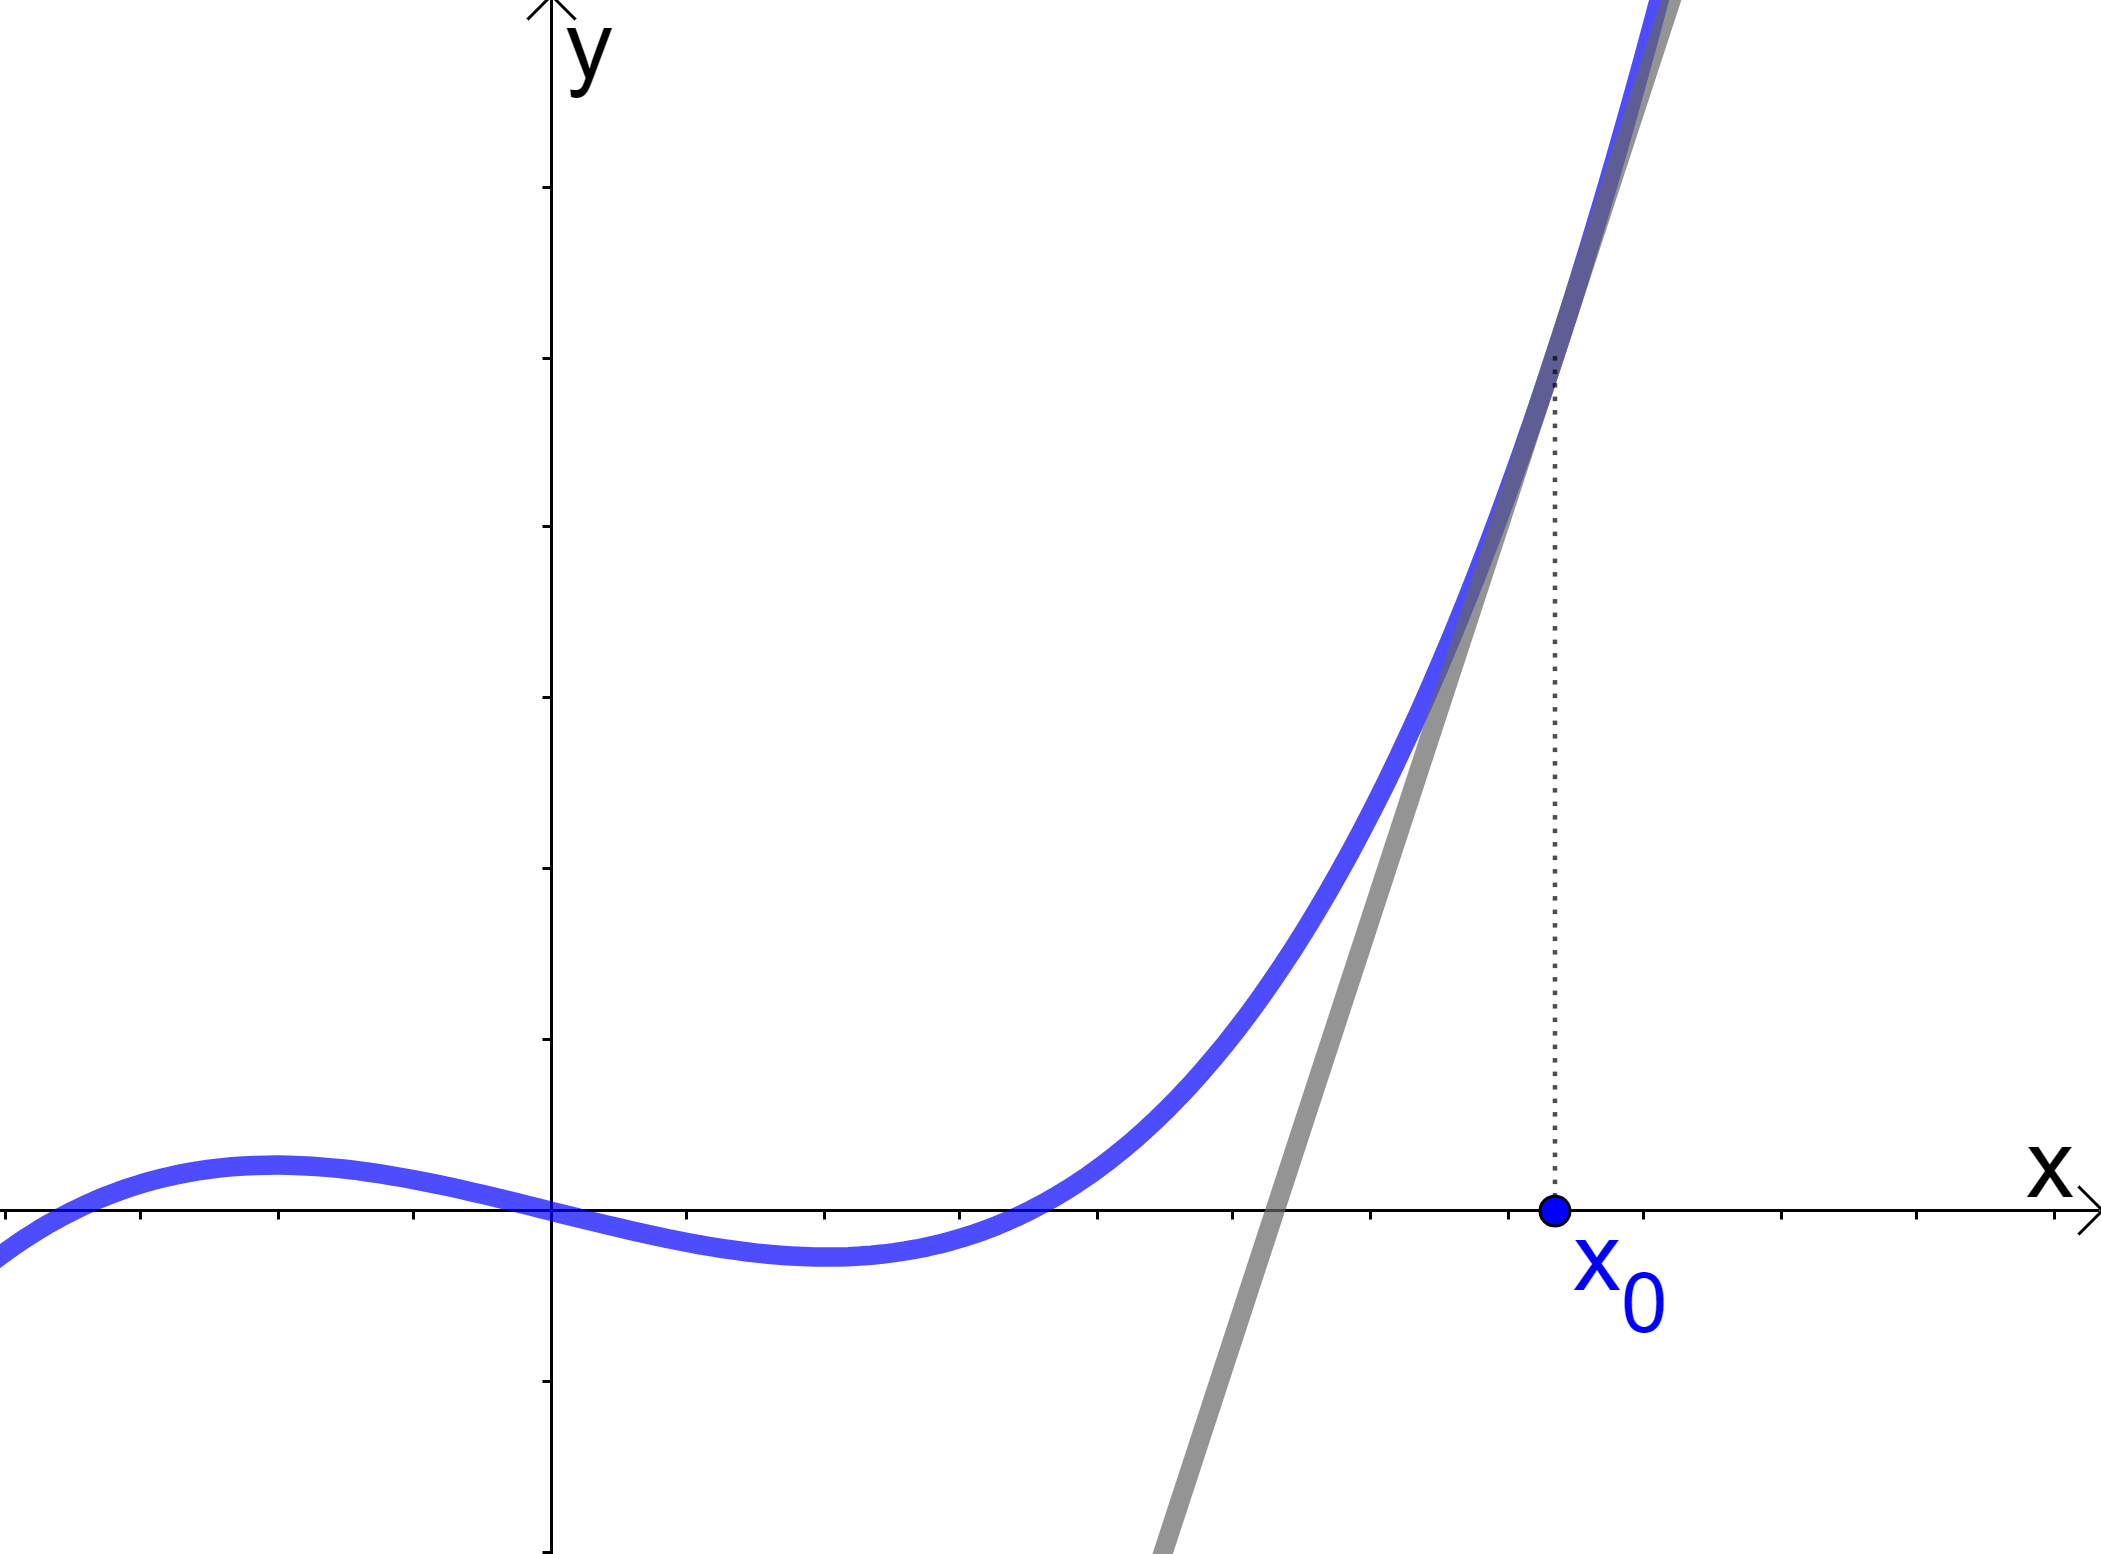
\includegraphics[width=\textwidth]
  {../Mathematik_1/Bilder/newton_tangente_startwert.png}
\end{minipage}\hfill
\begin{minipage}{0.32\textwidth}
  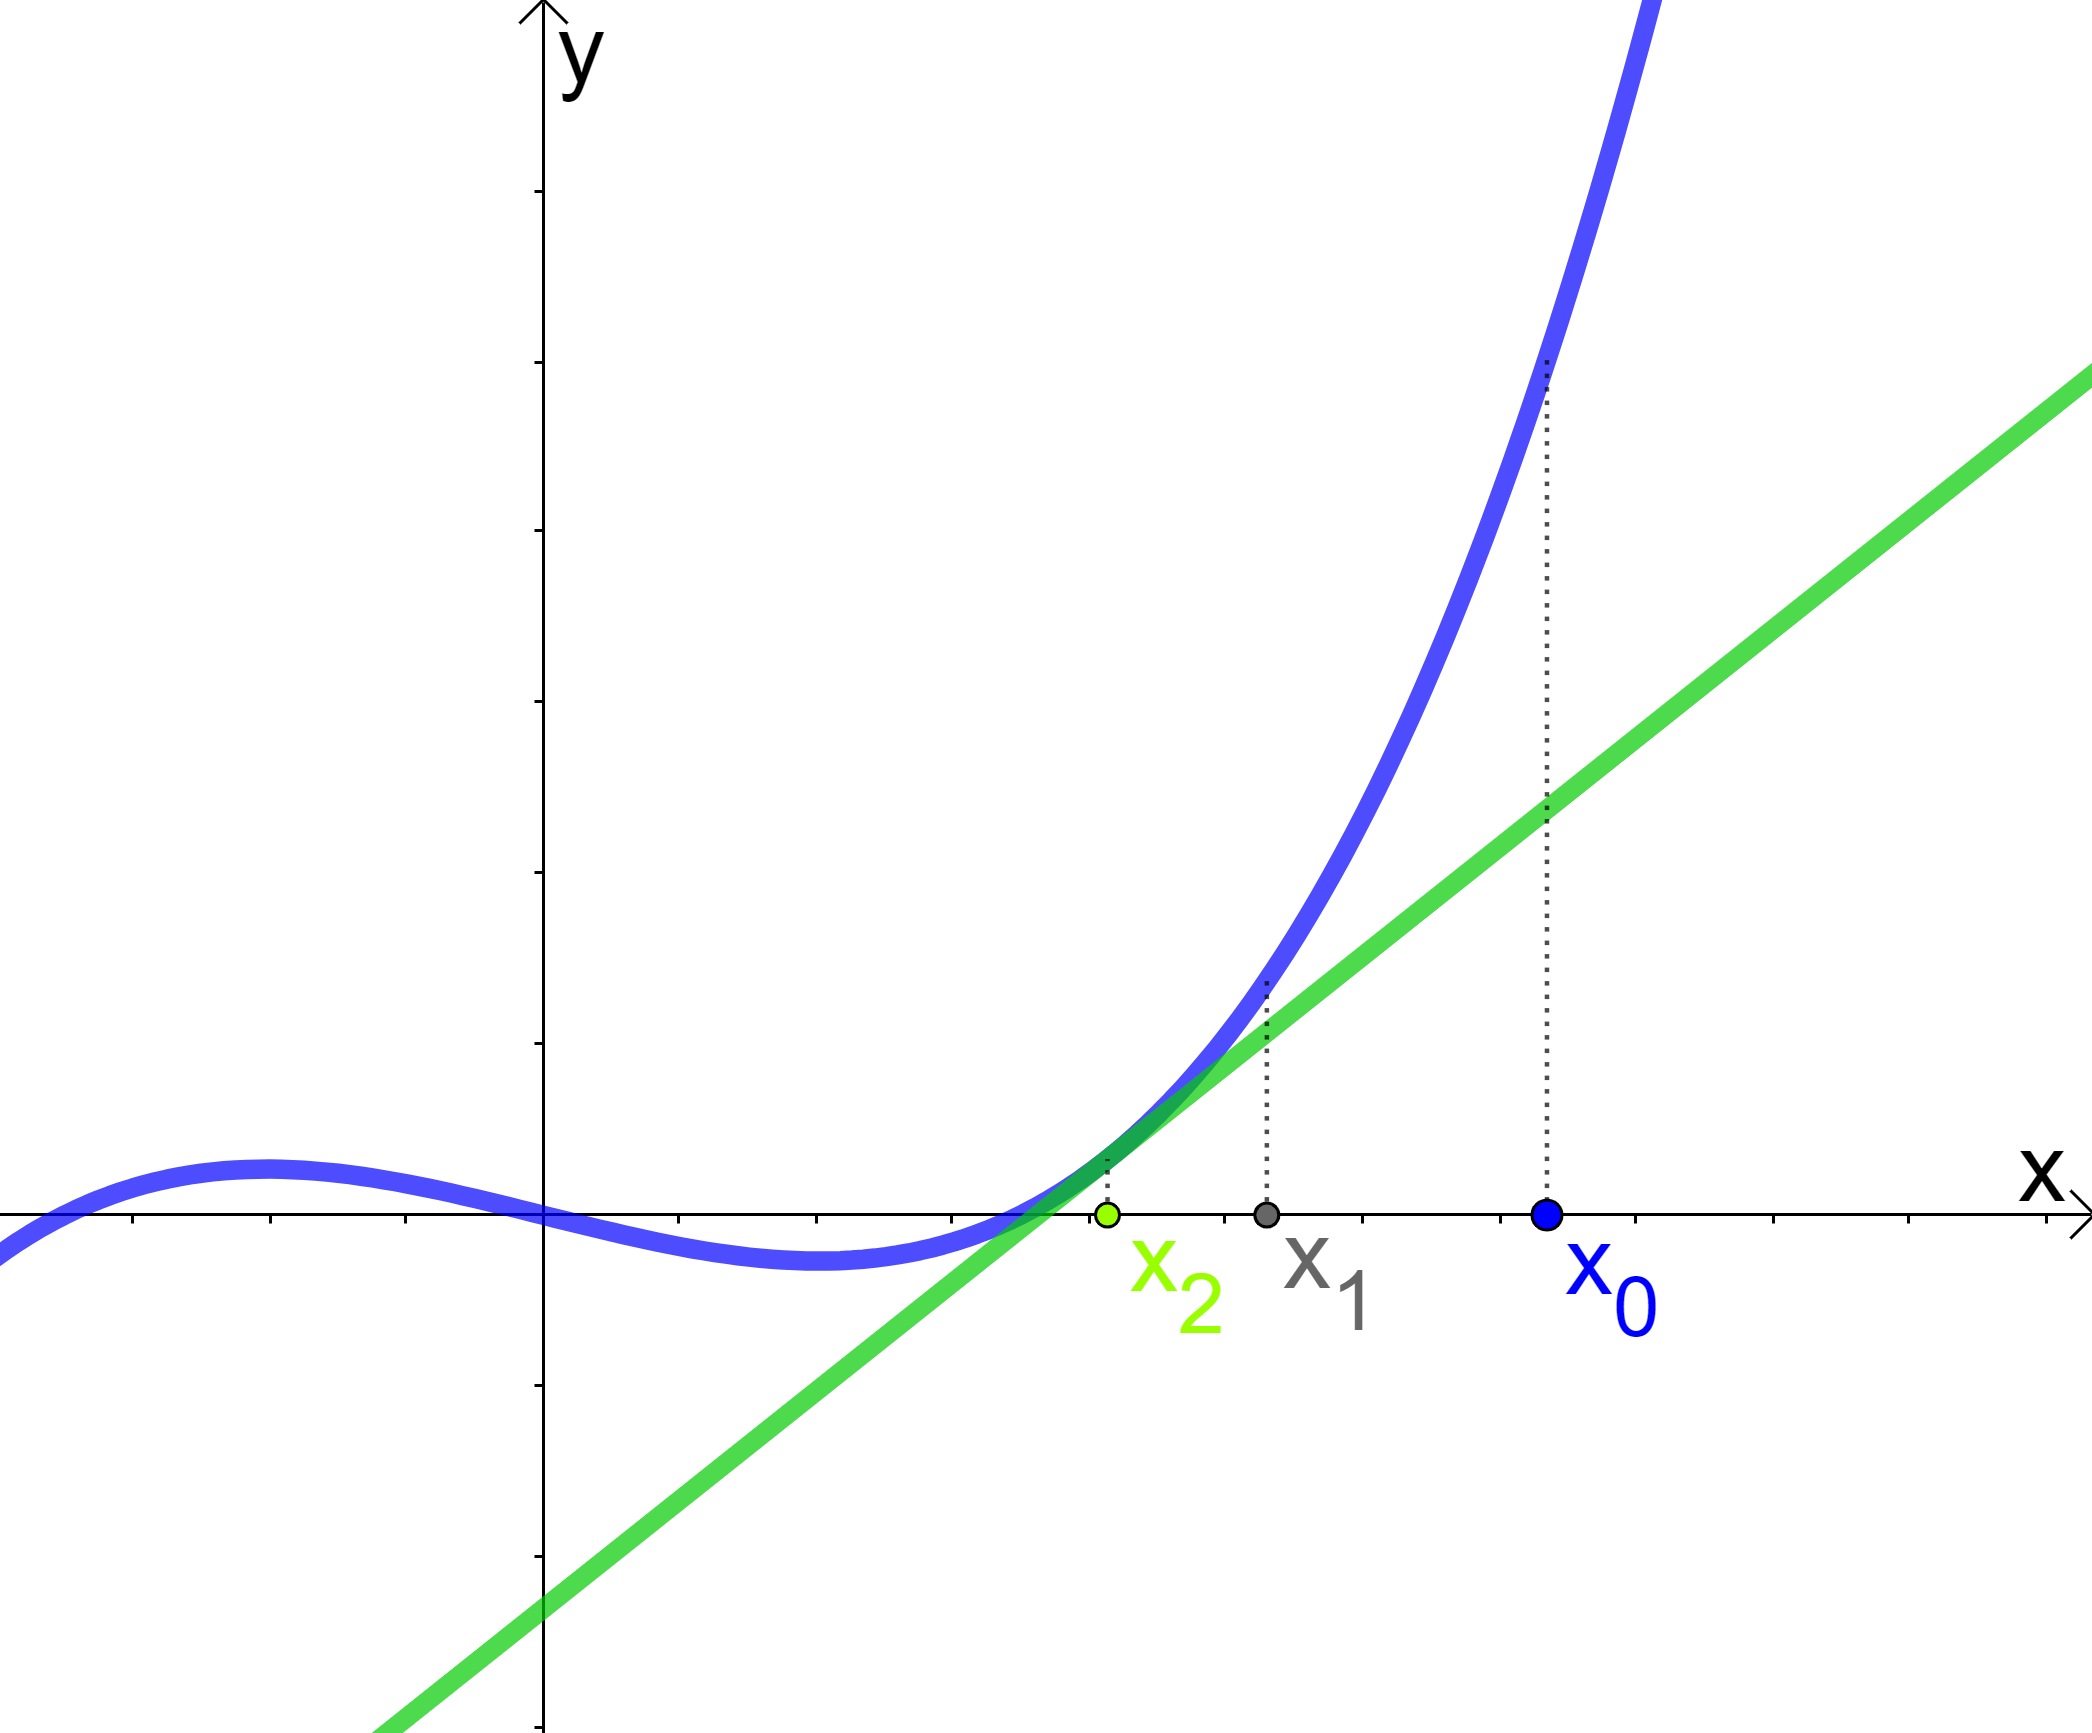
\includegraphics[width=\textwidth]
  {../Mathematik_1/Bilder/newton_tangente_zweite_iteration.png}
\end{minipage}\hfill
\begin{minipage}{0.32\textwidth}
  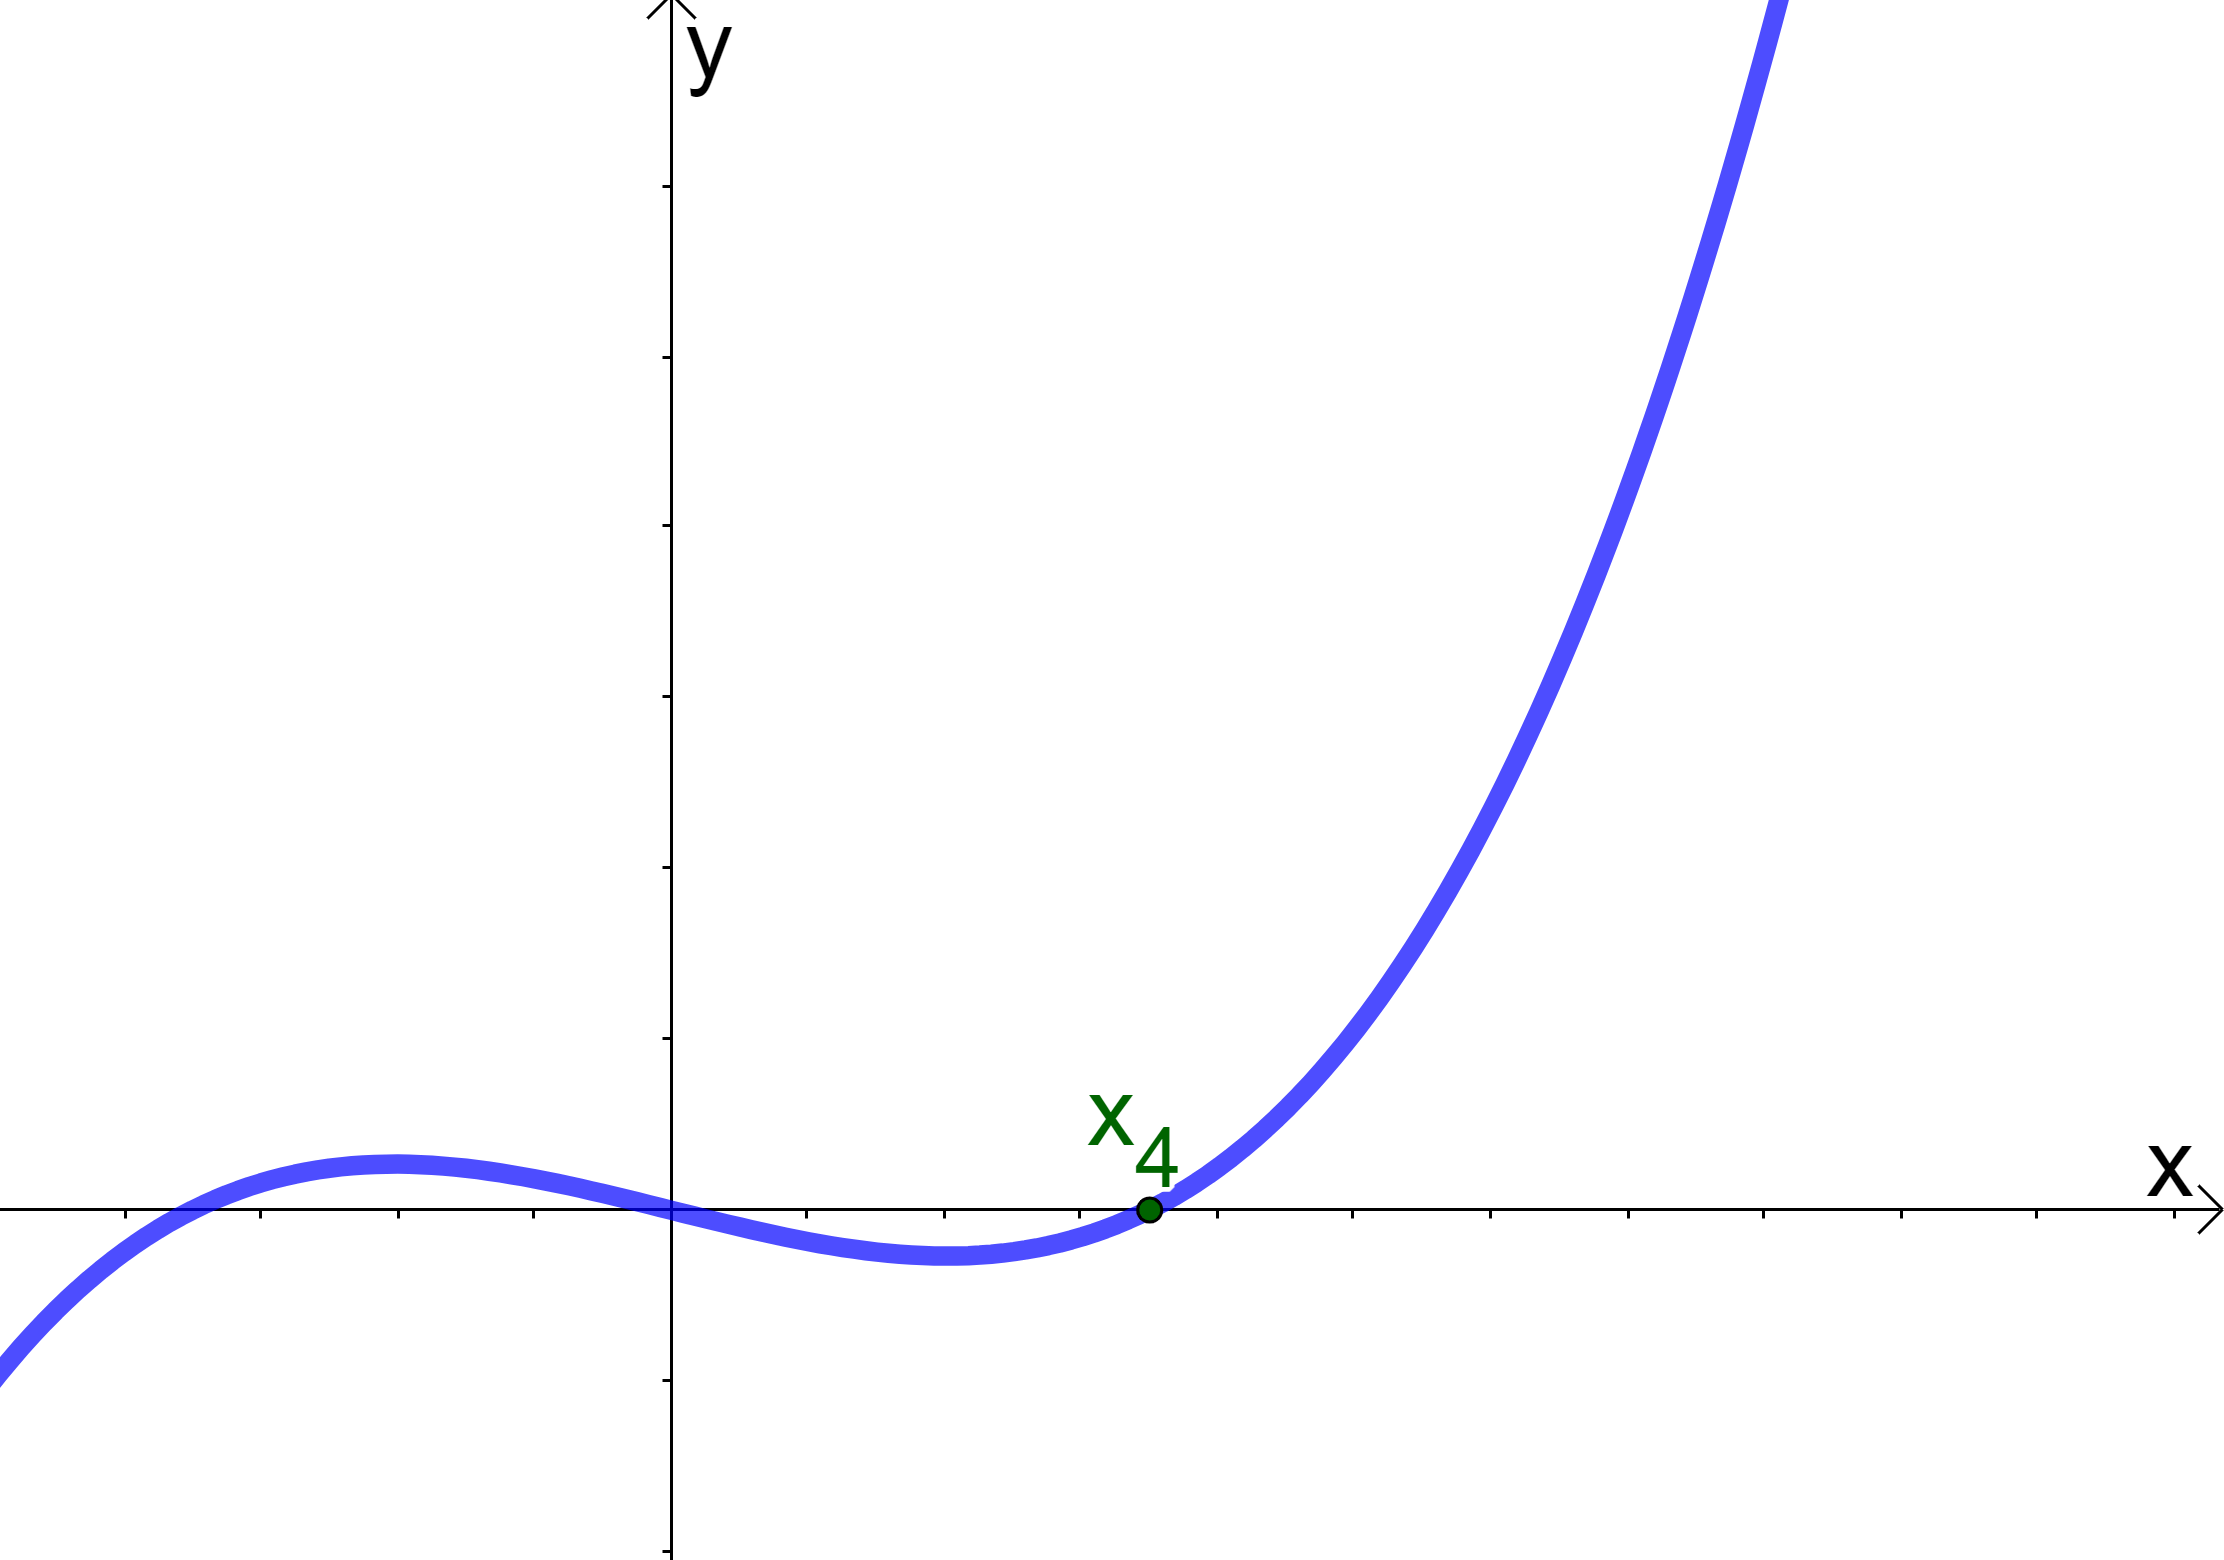
\includegraphics[width=\textwidth]
  {../Mathematik_1/Bilder/newton_naeherung_vierte_iteration.png}
\end{minipage}
\end{exabox}

Die Bildfolge zeigt die wiederholte Linearisierung geometrisch:
An jedem N�herungswert wird die Tangente gebildet. Deren Schnittpunkt mit
der \(x\)-Achse liefert den n�chsten N�herungswert.

Damit zeigt das Newton-Verfahren ein grundlegendes Vorgehen der Numerik:
Ein nichtlineares Problem wird lokal durch ein lineares Problem ersetzt,
das lineare Problem wird gel�st, und anschlie�end wird um die neue
N�herung erneut linearisiert.


\subsubsection*{Abbruch und m�gliche Schwierigkeiten}

In einer numerischen Rechnung kann die Iteration nicht unbegrenzt
fortgesetzt werden. Ein m�gliches Abbruchkriterium ist
\[
|x_{k+1}-x_k|<\varepsilon.
\]
Alternativ kann gepr�ft werden, ob der Funktionswert bereits hinreichend
klein ist:
\[
|f(x_k)|<\varepsilon.
\]

Beide Kriterien messen unterschiedliche Aspekte: Das erste beobachtet,
ob sich die N�herungswerte noch wesentlich ver�ndern, das zweite, wie gut
die aktuelle N�herung die Gleichung \(f(x)=0\) erf�llt.

Das Newton-Verfahren konvergiert nicht f�r jeden Startwert. Besonders
problematisch sind Stellen, an denen
\[
f'(x_k)\approx0.
\]
Die Tangente verl�uft dort nahezu horizontal, sodass der Quotient
\[
\frac{f(x_k)}{f'(x_k)}
\]
sehr gro� werden kann. Der n�chste Newton-Schritt kann dadurch weit vom
gesuchten Bereich wegf�hren.


\begin{exabox}{Schlechter Startwert}{}
\begin{minipage}{0.4\textwidth}
  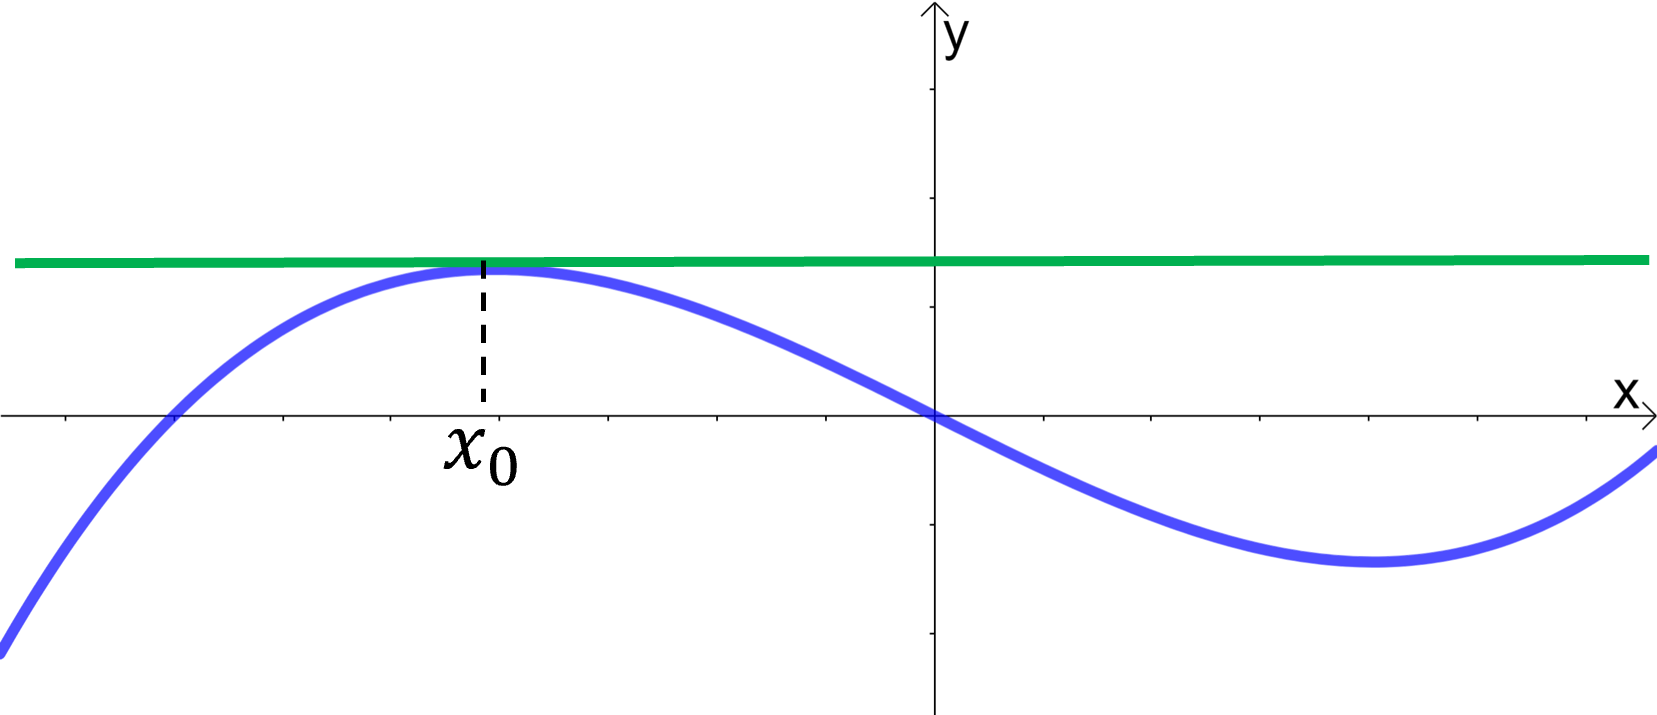
\includegraphics[width=\textwidth]
  {../Mathematik_1/Bilder/newton_problematische_flache_tangente.png}
\end{minipage}\hfill
\begin{minipage}{0.58\textwidth}
Ist die Tangente am aktuellen N�herungswert nahezu horizontal, kann ihr
Schnittpunkt mit der \(x\)-Achse sehr weit entfernt liegen. Die lokale
Linearisierung wird dann au�erhalb des Bereichs verwendet, in dem sie die
Funktion gut approximiert, und der Newton-Schritt kann unbrauchbar werden.
\end{minipage}
\end{exabox}

Gerade dieses m�gliche Scheitern macht noch einmal deutlich, weshalb das
Wort \emph{lokal} entscheidend ist: Eine Tangente beschreibt eine
nichtlineare Funktion nur in der N�he ihres Ber�hrpunktes gut.


% =========================================================
\subsubsection*{Konvergenz des Newton-Verfahrens (+)}

Unter geeigneten Voraussetzungen konvergiert das Newton-Verfahren in der
N�he einer einfachen Nullstelle besonders schnell.

Ist \(x^\ast\) eine Nullstelle mit
\[
f(x^\ast)=0,
\qquad
f'(x^\ast)\neq0,
\]
und ist \(f\) in einer Umgebung von \(x^\ast\) hinreichend glatt, so
konvergiert die Newton-Folge bei einem ausreichend guten Startwert
typischerweise \textbf{quadratisch} gegen \(x^\ast\).

F�r den Fehler
\[
e_k=x_k-x^\ast
\]
bedeutet dies lokal eine Beziehung der Form
\[
|e_{k+1}|
\le
C|e_k|^2.
\]

Ist der Fehler bereits klein, wird er im n�chsten Schritt also ungef�hr
quadriert. Dadurch kann sich die Zahl der korrekten Dezimalstellen in der
N�he der L�sung von einem Schritt zum n�chsten ungef�hr verdoppeln.


\begin{exabox}{Newton-Verfahren f�r \(x^3=7\)}{}

Die Gleichung
\[
x^3=7
\]
wird als Nullstellenproblem
\[
f(x)=x^3-7=0
\]
geschrieben. Wegen
\[
f'(x)=3x^2
\]
lautet die Newton-Iteration
\begin{eqnarray*}
x_{k+1}
&=&
x_k-\frac{x_k^3-7}{3x_k^2}\\[1ex]
&=&
\frac23x_k+\frac{7}{3x_k^2}.
\end{eqnarray*}

Bei einem geeigneten Startwert n�hert sich die Folge sehr schnell der
Nullstelle
\[
x^\ast=\sqrt[3]{7}.
\]
\end{exabox}


% =========================================================

\noindent\textbf{Zusammenfassung:}
Die Beispiele dieses Abschnitts beruhen auf derselben Grundidee.
Differenzierbarkeit erlaubt es, eine nichtlineare Funktion lokal durch
ihre Tangente zu ersetzen. Aus diesem einfachen Gedanken entstehen sehr
unterschiedliche Werkzeuge:

\[
\begin{array}{rcl}
\text{Funktionswert} &\longrightarrow& \text{Tangentenapproximation},\\[0.5ex]
\text{Grenzwert} &\longrightarrow& \text{Vergleich lokaler �nderungsraten},\\[0.5ex]
\text{diskrete Daten} &\longrightarrow& \text{Differenzenquotienten},\\[0.5ex]
\text{nichtlineare Gleichung} &\longrightarrow& \text{Newton-Verfahren}.
\end{array}
\]

Damit ist die Linearisierung nicht nur eine geometrische Interpretation
der Ableitung. Sie ist ein grundlegendes Prinzip, mit dem nichtlineare
Probleme lokal durch einfachere lineare Probleme approximiert werden.
 \newpage % Lokale Linearit�t
\setcounter{exercise}{0} 
\ifintegriereaufgaben
\section*{Lokale Linearit�t Aufgaben}\label{MA1-lokale-linearitaet-aufgaben}

	Regeln und Beispiele, die zur Bearbeitung der Aufgaben hilfreich sind, finden Sie im Skript\wennreferenzvorhanden{MA1-lokale-linearitaet}{ (Abschnitt \abschnittsverweis{MA1-lokale-linearitaet})} und, falls Sie nicht weiterkommen, schauen Sie \hyperref[MA1-lokale-linearitaet-loesungen]{hier}.
\else
\section{Lokale Linearit�t Aufgaben}\label{MA1-lokale-linearitaet-aufgaben}

	Regeln und Beispiele, die zur Bearbeitung der Aufgaben hilfreich sind, finden Sie im Skript und, falls Sie nicht weiterkommen, schauen Sie \hyperref[MA1-lokale-linearitaet-loesungen]{hier}.

\fi 

\begin{exercisebox}[Zentrale Differenz und zweite Differenz]
	\begin{itemize}
		\item[(a)] Zeigen Sie, dass sich die erste Ableitung von Polynomen vom Grad $2$ mit der zentralen Differenz exakt berechnen l��t.
		\item[(b)] Zeigen Sie, dass sich die zweite Ableitung von Polynomen vom Grad $4$ mit der zweiten Differenz exakt berechnen l��t.
	\end{itemize}
\end{exercisebox}

\begin{exercisebox}[Bestapproximation]
	Gegeben seien Messungen $x_1, x_2, \cdots, x_n\in\mathbb R$, $n\in \mathbb N$ einer Gr��e $x\in \mathbb R$. Gesucht ist eine Approximation $\tilde x\in \mathbb R$, deren Abstand zu allen Messwerten gleichzeitig minimal ist, also 
	\[ \sum\limits_{k=1}^n |x- x_k|^2 \stackrel{!}{=} \mathrm{min}\,.\]
		Bestimmen Sie eine Formel f�r $\tilde x$. 
\end{exercisebox} 

\begin{exercisebox}[Taylorentwicklung]
	Gegeben sei die Funktion $f: x\mapsto \cos(x)$. Bestimmen Sie die Taylorentwicklung $T_7$ von $f$ an der Stelle $x_0=0$ und sch�tzen Sie den Betrag des Lagrangeschen Restglieds $R_8$ im Intervall $x\in I= [ -\pi/6, \pi/6]$ ab. 
\end{exercisebox} 

\begin{exercisebox}[Interpolation (Wiederholung)]
Gegeben sind die Punkte 
\begin{center}
	\begin{tabular}{c|cccc}
		$i$ & $0$ & $1$ & $2$ & $3$ \\
		\hline
		$x_i$ & $-3$ & $-1$ & $0$ & $2$ \\
		\hline
		$y_i$ & $-3$ & $1$ & $0$ & $82$ \\
	\end{tabular}
\end{center}
\begin{itemize}
	\item[(a)]  Bestimmen Sie den Grad $n$ des Interpolationspolynoms. 
	\item[(b)]  Bestimmen Sie das lineare Gleichungssystem f�r die Koeffizienten des Interpolationspolynoms in der Darstellung \[ p(x) =a_nx^n+\cdots +a_1 x+a_0\] und l�sen Sie es.
	%\item[(c)]  Bestimmen Sie den Wert des Polynoms an der Zwischenstelle $\tilde x= 1$.
	%\item[(d)]  Bestimmen Sie das lineare Gleichungssystem f�r die Koeffizienten des Interpolationspolynoms in der Darstellung \[ q(x) =c_0+c_1(x-x_0) +c_2(x-x_0)(x-x_1) +\cdots +c_n(x-x_0)\cdots(x-x_{n-1})\] und l�sen Sie es mit Matlab.
	%\item[(e)]  Berechnen Sie den Wert des Polynoms $q$ an der Zwischenstelle $\tilde x= 1$. Wie k�nnnen Sie den Wert effizient berechnen?
\end{itemize}
\end{exercisebox}


\begin{exercisebox}[Interpolation (Wiederholung)]
	Eine Funktion der Form \[ f: x \mapsto \frac{a_0}{2} + a_1 \cos(x) + b_1 \sin(x) \,,\] soll durch die Punkte $(x_i, y_i), i=1,2,3$ mit \[ (0|1), \, (\pi/6|-1),\, (\pi/2|-3)\] gelegt werden. Bestimmen Sie ein Gleichungssystem f�r die Koeffizienten $a_0, a_1, b_1$ und l�sen Sie es.

\end{exercisebox} 

%\begin{exercisebox}[Lineare Regression (Wiederholung)]
%  F�r Wohnungen verlangt eine Baufirma die angegebenen Kaufpreise. Wie lautet die lineare Regressionsgerade? Berechnen Sie den Kaufpreis f�r eine $88\mathrm{m}^2$ gro�e Wohnung.
%  \begin{center}
%  \begin{tabular}{c|cccc}
%    Wohnfl�che in $\mathrm{m}^2$ & $40$ & $60$ & $80$ & $100$\\ 
%    \hline
%    Preis in $\mathrm{T} $\euro & $120$ & $165$ & $210$ & $255$ 
%  \end{tabular}
%  \end{center}
%
%  %\hspace{0.3cm}
%  %\newline
%  %{\bf L�sung:}
%  %F�hren wir die Variable $x$ zur Bezeichnung der Wohnfl�che und die Variable $y$ zur Bezeichnung des Preises ein. Es gilt \[ \frac{\Delta y}{\Delta x} = \frac{y_{i+1}- y_i}{x_{i+1} - x_i} = \frac{ 4}{9 }\] und daas hei�t, dass der Preis linear von der Gr��e der Wohnung abh�ngt. Damit ist die Ausgleichsgerade die interpolierende Gerade mit der Gleichung \[ g(x) = \frac49 (x-40) + 120 \,.\]
%\end{exercisebox} 

 \newpage 
\setcounter{satz}{0} \setcounter{def}{0} \setcounter{exa}{0}  \section{Ableitungen und Funktionsverlauf}\label{MA1-ableitungen-und-funktionsverlauf}

\begin{table}[H]
  \centering
  \begin{tabularx}{\textwidth}{p{0.9\textwidth} p{0.1\textwidth}}
    \toprule
    \multicolumn{2}{c}{\textbf{�bersicht �ber Lernziele und Voraussetzungen}}\\
    \midrule
    \textbf{Lernziele} &\\[.5\normalbaselineskip]
\tabitem das Vorzeichen von \(f^\prime\) als Aussage �ber lokales Steigungsverhalten interpretieren &\\
\tabitem Vorzeichenwechsel von \(f'\) mit lokalen Extrema von \(f\) in Verbindung bringen &\\
\tabitem das Vorzeichen von \(f^{''}\) als Aussage �ber lokales Kr�mmungsverhalten interpretieren &\\
    \tabitem Vorzeichenwechsel von \(f''\) mit Wendestellen in Verbindung bringen &\\
    \midrule
    \textbf{Voraussetzungen} &\\[.5\normalbaselineskip]
    \tabitem Definition der Ableitung & \abschnittsverweis{MA1-stetigkeit-und-differenzierbarkeit}\\
    \tabitem Berechnung von Ableitungen & \abschnittsverweis{MA1-ableitungsregeln}\\
    \tabitem Lokale Linearit�t & \abschnittsverweis{MA1-lokale-linearitaet}\\
    \bottomrule
  \end{tabularx}
\end{table}

\ifintegriereaufgaben
\noindent �bungsaufgaben zum Thema:
\hyperref[MA1-ableitungen-und-funktionsverlauf-aufgaben]{Aufgaben}
\vspace{0.3cm}
\hrule
\fi


% =========================================================
\subsection{Ableitungen beschreiben lokalen Funktionsverlauf}

Die Ableitung einer Funktion ist selbst wieder eine Funktion. W�hrend
\(f\) die betrachtete Gr��e beschreibt, enth�lt \(f'\) Informationen
dar�ber, wie sich diese Gr��e lokal ver�ndert.

Damit er�ffnet die Differentialrechnung zwei unterschiedliche, aber eng
miteinander verbundene Sichtweisen auf eine Funktion.

Die \textbf{Linearisierung} beantwortet die Frage, durch welche einfache
Funktion \(f\) in unmittelbarer Umgebung eines Punktes approximiert
werden kann. Die Ableitungsfunktionen \(f'\), \(f''\), \ldots{} erlauben
dagegen qualitative Aussagen dar�ber, wie sich der Funktionsverlauf lokal
verh�lt.

Die erste Ableitung beschreibt die lokale �nderung von \(f\):
\[
f'(x)>0
\quad\Longrightarrow\quad
f\text{ w�chst lokal},
\]
w�hrend
\[
f'(x)<0
\quad\Longrightarrow\quad
f\text{ f�llt lokal}.
\]

Die zweite Ableitung beschreibt, wie sich diese lokale �nderungsrate
selbst ver�ndert. Sie gibt damit Auskunft dar�ber, ob die Steigung
zunimmt oder abnimmt und wie sich der Graph kr�mmt.

Ableitungen liefern somit nicht nur Zahlen. Ihre Vorzeichen und
Vorzeichenwechsel enthalten qualitative Informationen �ber den Verlauf
der urspr�nglichen Funktion.


% =========================================================
\subsection{Die erste Ableitung: Wachstum und Abnahme}

Ist \(f'(x_0)>0\), so besitzt die Tangente an \(f\) in \(x_0\) eine
positive Steigung. In hinreichend kleiner Umgebung von \(x_0\) nimmt
die Funktion daher zu.

Entsprechend bedeutet \(f'(x_0)<0\), dass die Tangente eine negative
Steigung besitzt und die Funktion lokal abnimmt.

Aus einer punktweisen Aussage wird eine Aussage �ber einen ganzen
Funktionsabschnitt, wenn das Vorzeichen der Ableitung auf einem Intervall
bekannt ist.

\begin{theorembox}{Vorzeichen von \(f'\) und Monotonie}{}
Es sei \(f\) auf einem Intervall \(I\) differenzierbar.

Gilt
\[
f'(x)>0
\qquad\text{f�r alle }x\in I,
\]
so ist \(f\) auf \(I\) streng monoton wachsend.

Gilt
\[
f'(x)<0
\qquad\text{f�r alle }x\in I,
\]
so ist \(f\) auf \(I\) streng monoton fallend.
\end{theorembox}

Die Ableitungsfunktion liefert damit eine qualitative Beschreibung des
Funktionsverlaufs, ohne dass alle Funktionswerte von \(f\) einzeln
betrachtet werden m�ssen.

Besonders interessant sind Stellen, an denen sich das Vorzeichen von
\(f'\) �ndert.

Wechselt \(f'\) von positiv nach negativ, so geht die Funktion lokal von
Wachstum zu Abnahme �ber:
\[
f':\quad +\longrightarrow-
\qquad\Longrightarrow\qquad
\text{lokales Maximum}.
\]

Wechselt \(f'\) von negativ nach positiv, so geht die Funktion lokal von
Abnahme zu Wachstum �ber:
\[
f':\quad -\longrightarrow+
\qquad\Longrightarrow\qquad
\text{lokales Minimum}.
\]

An einer solchen Extremstelle besitzt eine differenzierbare Funktion eine
horizontale Tangente. F�r einen inneren Punkt \(x_0\) gilt daher
notwendigerweise
\[
f'(x_0)=0.
\]

Die Umkehrung gilt jedoch nicht: Eine horizontale Tangente allein bedeutet
noch nicht, dass dort ein Extremum vorliegt.


\begin{exabox}{Der Vorzeichenwechsel entscheidet}{}

\begin{minipage}{0.58\textwidth}
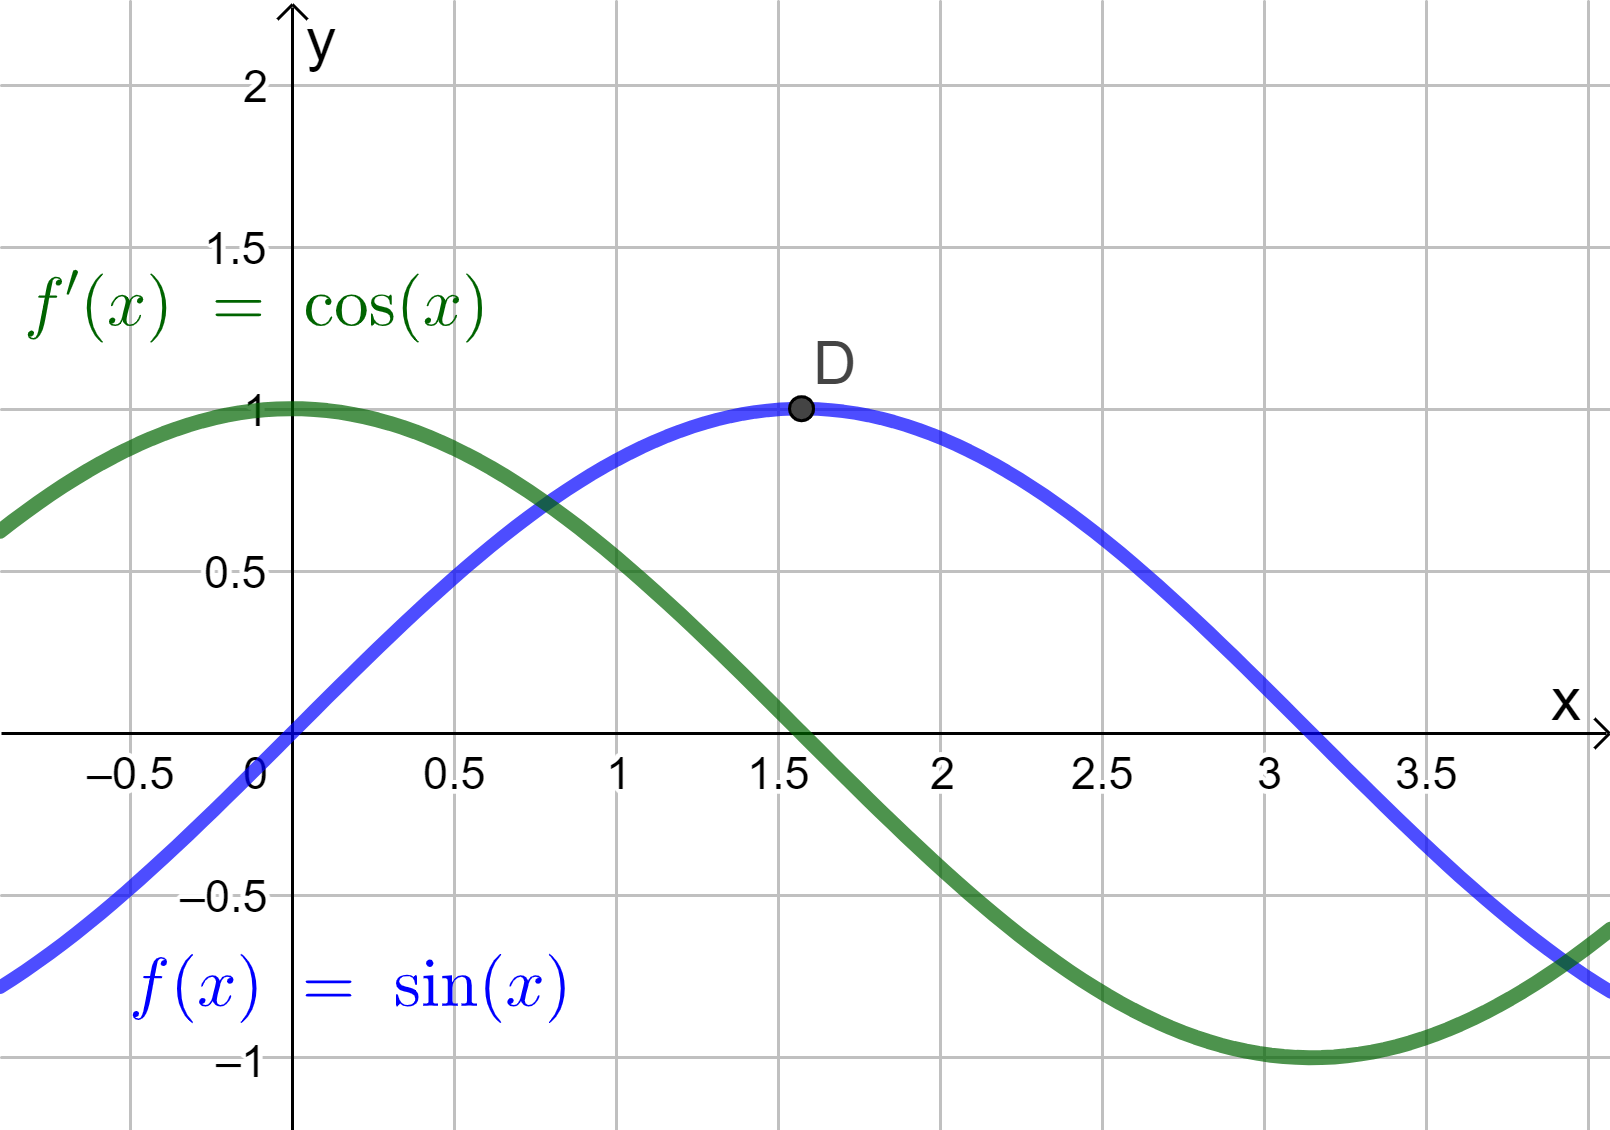
\includegraphics[width=\textwidth]
{../Mathematik_1/Bilder/ableitung_sinus_kosinus.png}
\end{minipage}
\hfill
\begin{minipage}{0.40\textwidth}

F�r
\[
f(x)=\sin(x)
\]
gilt
\[
f'(x)=\cos(x).
\]

Bei \(x_0=\pi/2\) verschwindet die Ableitung und wechselt ihr Vorzeichen:
\[
+\longrightarrow-.
\]

Die Sinusfunktion geht dort von Wachstum zu Abnahme �ber. Sie besitzt
folglich ein lokales Maximum.
\end{minipage}

\vspace{2ex}

\begin{minipage}{0.58\textwidth}
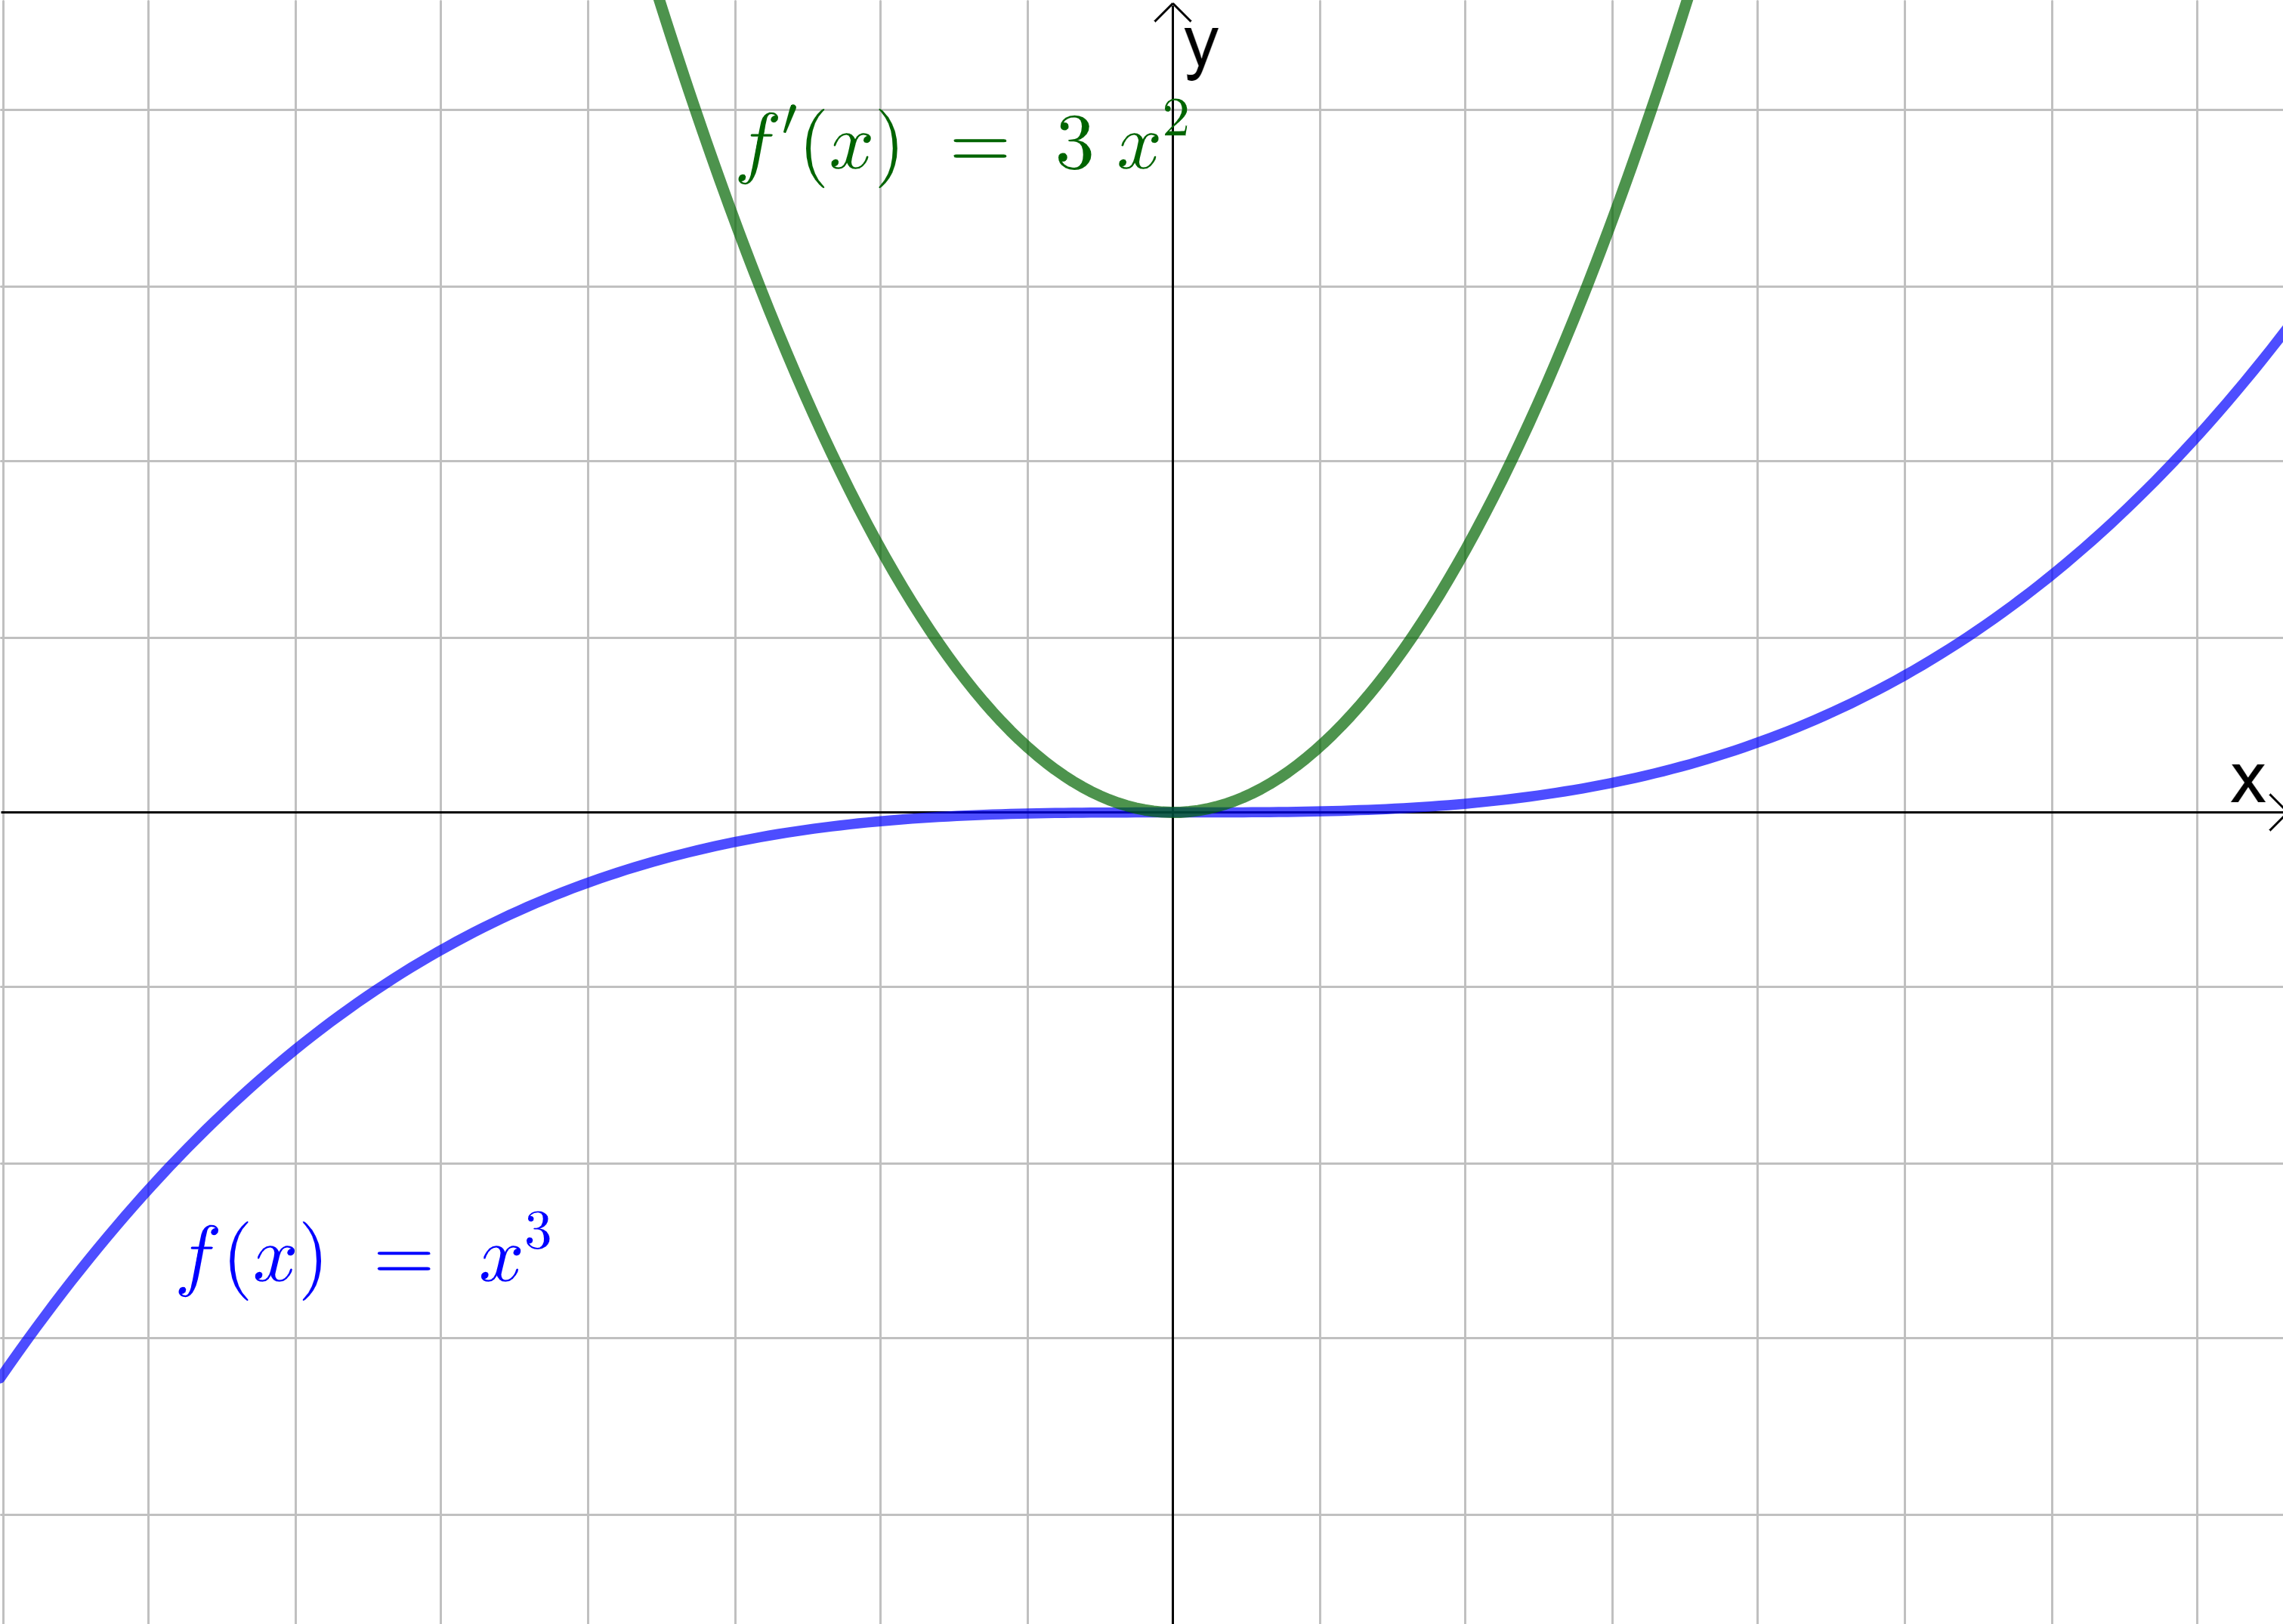
\includegraphics[width=\textwidth]
{../Mathematik_1/Bilder/extremstellen_potenz_drei_gegenbeispiel.png}
\end{minipage}
\hfill
\begin{minipage}{0.40\textwidth}

F�r
\[
f(x)=x^3
\]
gilt
\[
f'(x)=3x^2.
\]

Auch hier ist
\[
f'(0)=0.
\]
Die Ableitung bleibt jedoch auf beiden Seiten von \(0\) positiv. Die
Funktion w�chst also vor und nach \(x_0=0\).

Es liegt kein lokales Extremum vor.
\end{minipage}

\end{exabox}

Das Beispiel zeigt einen wichtigen Unterschied: Die Gleichung
\[
f'(x_0)=0
\]
liefert zun�chst nur eine Stelle mit horizontaler Tangente. Erst das
lokale Verhalten von \(f'\) um \(x_0\) zeigt, was dort mit der Funktion
geschieht.


% =========================================================
\subsection{Die zweite Ableitung: Wie ver�ndert sich die Steigung?}

Die erste Ableitung \(f'\) beschreibt die Steigung von \(f\). Die zweite
Ableitung
\[
f''=(f')'
\]
beschreibt daher, wie sich diese Steigung ver�ndert.

Ist
\[
f''(x)>0,
\]
so nimmt \(f'(x)\) lokal zu. Die Steigungen von \(f\) werden also gr��er.

Ist dagegen
\[
f''(x)<0,
\]
so nimmt \(f'(x)\) lokal ab. Die Steigungen von \(f\) werden kleiner.

Diese Aussage ist zun�chst unabh�ngig davon, ob \(f\) selbst gerade
steigt oder f�llt. Beispielsweise kann eine Funktion fallen und dabei
immer flacher werden. In diesem Fall ist
\[
f'(x)<0,
\qquad
f''(x)>0.
\]

Die Vorzeichen von \(f'\) und \(f''\) beschreiben also unterschiedliche
Eigenschaften:

\[
\begin{array}{ccl}
f'(x) &:& \text{Richtung der lokalen �nderung von }f,\\[0.5ex]
f''(x)&:& \text{�nderung dieser lokalen Steigung}.
\end{array}
\]

Geometrisch f�hrt die zweite Ableitung zur
\textbf{Kr�mmung} (\emph{curvature behaviour}) des Graphen.

\begin{theorembox}{Vorzeichen von \(f''\) und Kr�mmung}{}
Es sei \(f\) auf einem Intervall \(I\) zweimal differenzierbar.

Gilt
\[
f''(x)>0
\qquad\text{f�r alle }x\in I,
\]
so ist \(f\) auf \(I\) konvex.

Gilt
\[
f''(x)<0
\qquad\text{f�r alle }x\in I,
\]
so ist \(f\) auf \(I\) konkav.
\end{theorembox}

Eine �nderung des Vorzeichens von \(f''\) zeigt einen Wechsel des
Kr�mmungsverhaltens an. Eine solche Stelle hei�t
\textbf{Wendestelle} (\emph{inflection point} f�r den zugeh�rigen Punkt
des Graphen).

F�r eine hinreichend glatte Funktion gilt an einer inneren Wendestelle
notwendigerweise
\[
f''(x_0)=0.
\]

Wie schon bei der ersten Ableitung reicht das Verschwinden der Ableitung
allein jedoch nicht aus. Entscheidend ist wiederum das lokale Verhalten:
Das Vorzeichen von \(f''\) muss sich �ndern.


\begin{exabox}{Wendestelle als �nderung des lokalen Verhaltens}{}

\begin{minipage}{0.58\textwidth}
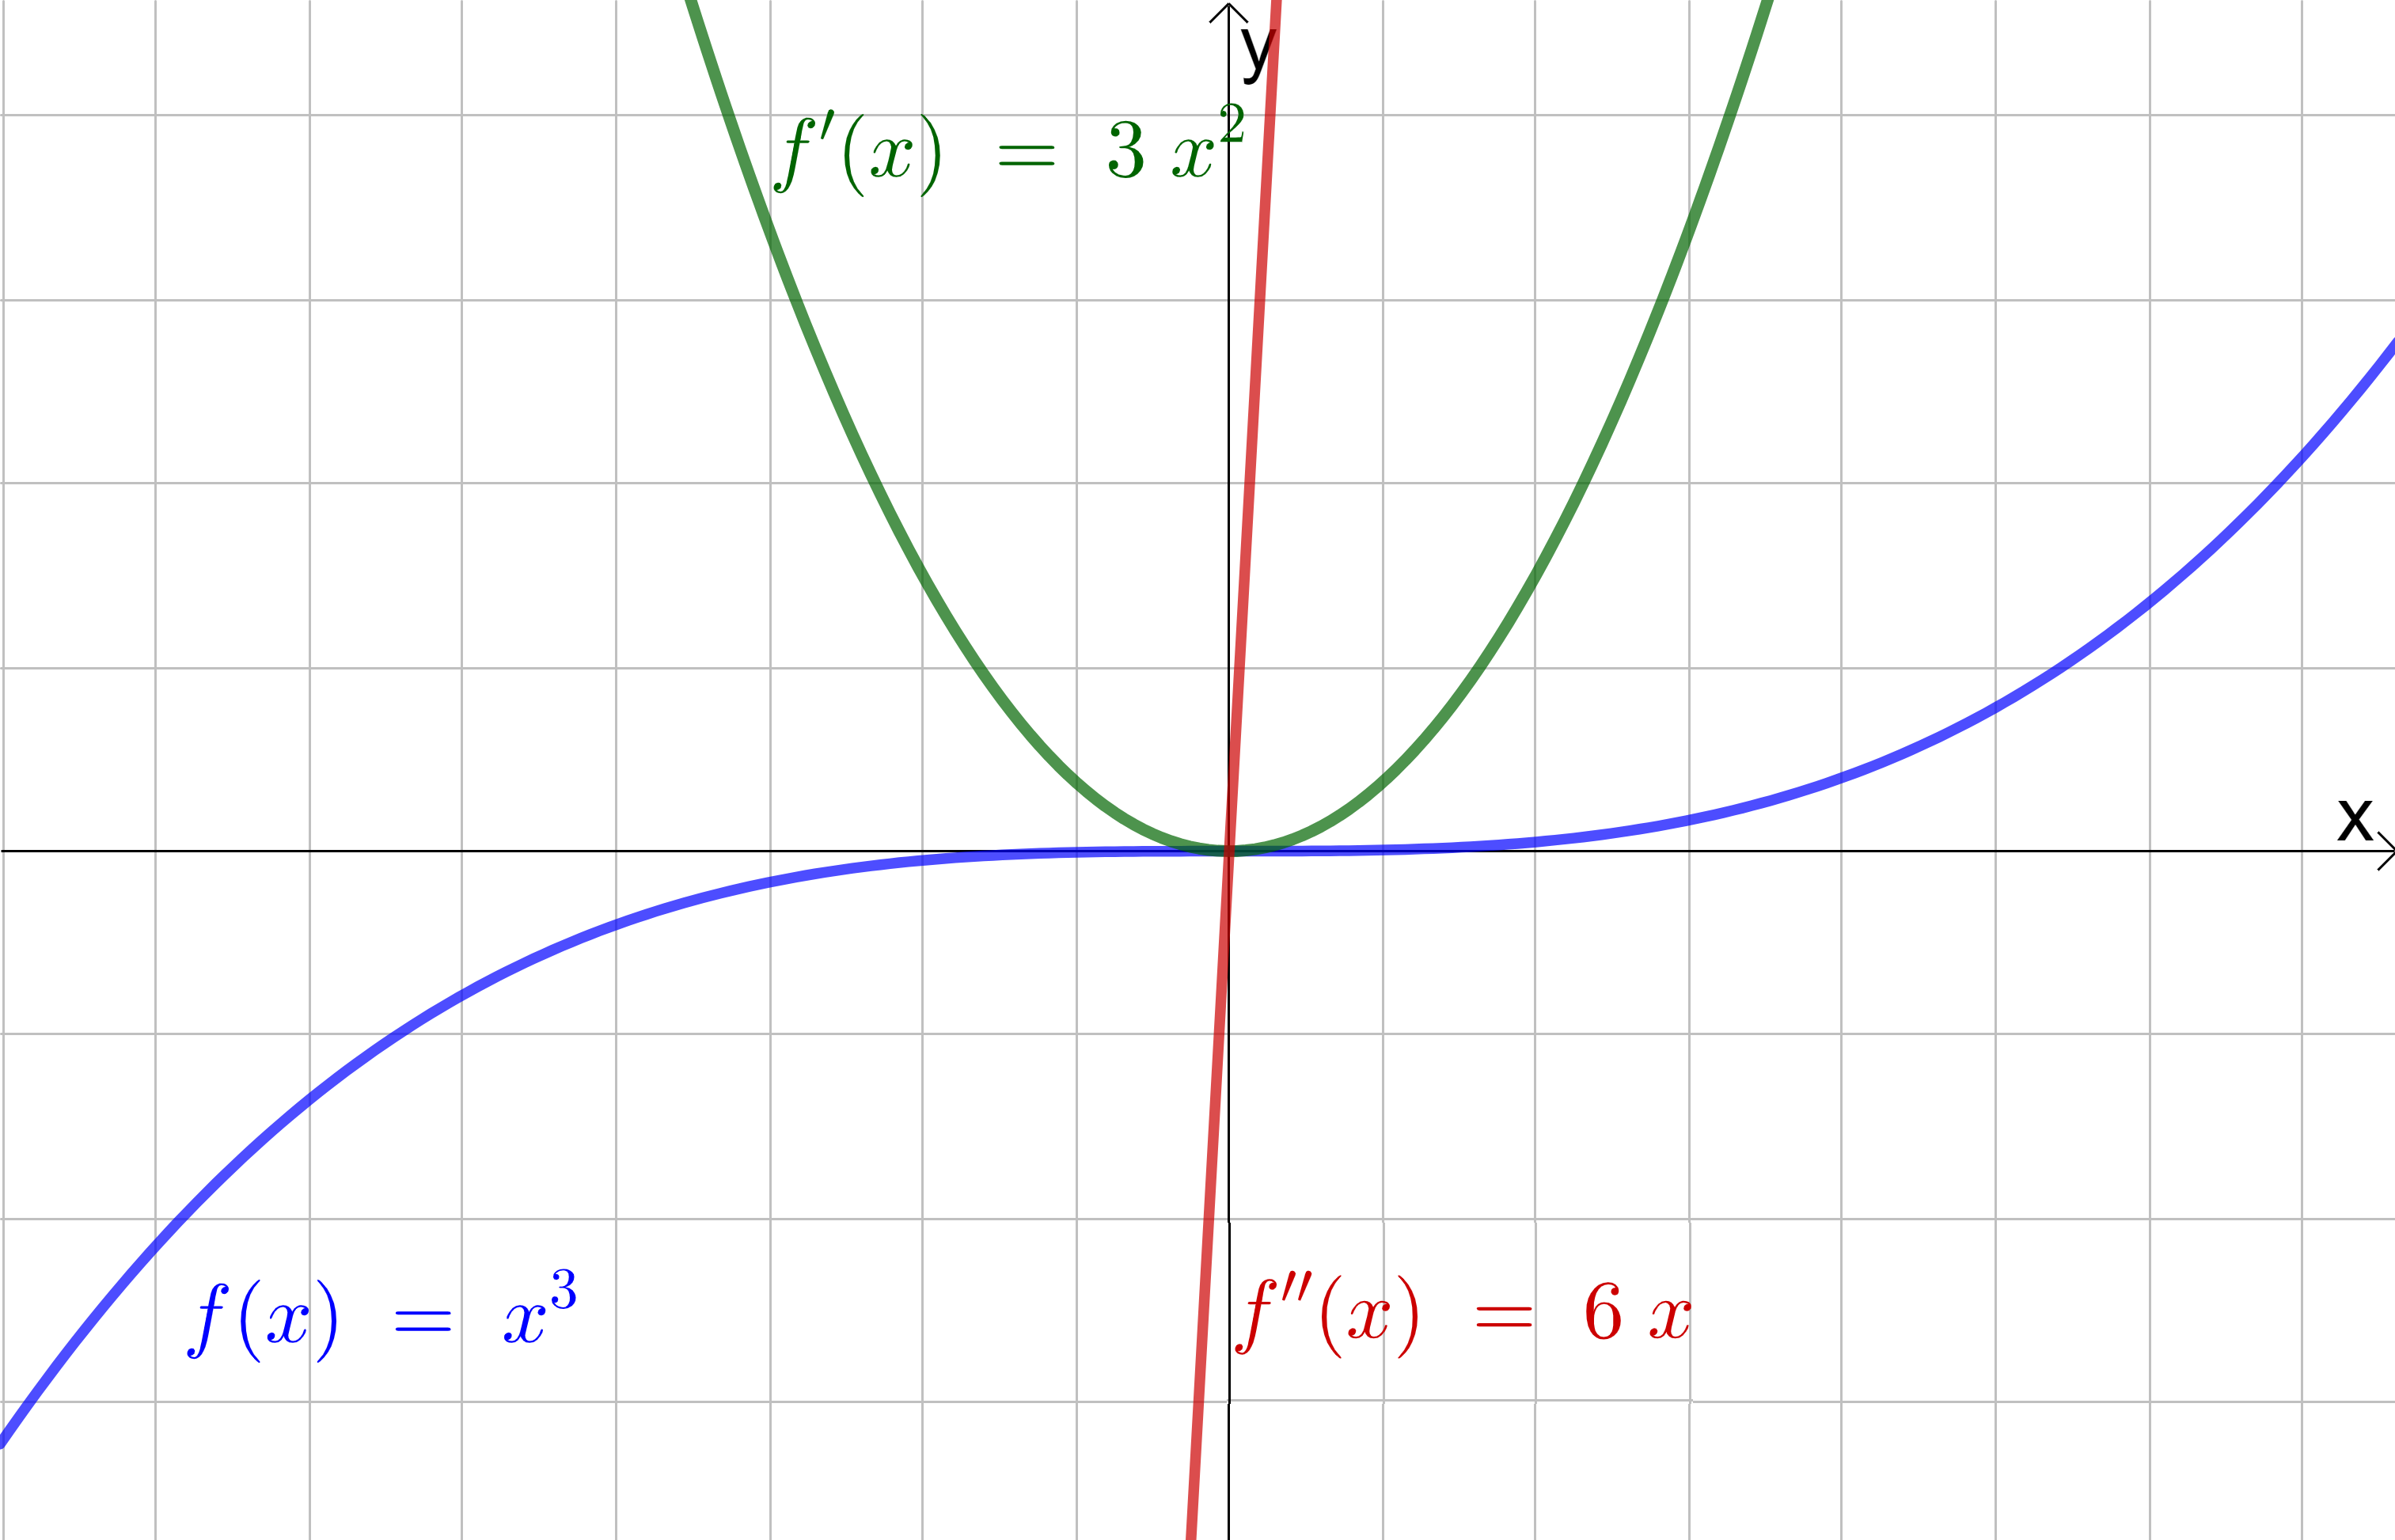
\includegraphics[width=\textwidth]
{../Mathematik_1/Bilder/wendestellen_potenz_drei_ableitungen.png}
\end{minipage}
\hfill
\begin{minipage}{0.40\textwidth}

F�r
\[
f(x)=x^3
\]
gilt
\[
f''(x)=6x.
\]

Damit ist
\[
f''(x)<0
\quad\text{f�r }x<0,
\]
und
\[
f''(x)>0
\quad\text{f�r }x>0.
\]

Die zweite Ableitung wechselt bei \(x_0=0\) ihr Vorzeichen. Dort �ndert
sich das Kr�mmungsverhalten der Funktion: \(x_0=0\) ist eine Wendestelle.
\end{minipage}

\end{exabox}


% =========================================================
\subsection{Ableitungen als qualitative Information}

Die ersten beiden Ableitungen lassen sich gemeinsam lesen. Dabei geht es
nicht in erster Linie darum, einzelne ausgezeichnete Punkte zu berechnen.
Vielmehr beschreiben \(f'\) und \(f''\), wie sich eine Funktion lokal
verh�lt.

F�r einen Punkt \(x\) liefern bereits die Vorzeichen
\[
f'(x)
\qquad\text{und}\qquad
f''(x)
\]
eine qualitative Charakterisierung.

\begin{center}
\begin{tabular}{c|c|c}
 & \(f''(x)>0\) & \(f''(x)<0\)\\
\hline
\(f'(x)>0\)
&
wachsend, Steigung nimmt zu
&
wachsend, Steigung nimmt ab
\\[0.5ex]
\(f'(x)<0\)
&
fallend, Steigung nimmt zu
&
fallend, Steigung nimmt ab
\end{tabular}
\end{center}

So bedeutet beispielsweise
\[
f'(x)>0,
\qquad
f''(x)<0,
\]
dass die Funktion zwar w�chst, ihre Steigung aber abnimmt: Der Graph
steigt weiter, wird dabei jedoch zunehmend flacher.

Dagegen bedeutet
\[
f'(x)<0,
\qquad
f''(x)>0,
\]
dass die Funktion f�llt, ihre Steigung aber zunimmt. Die Steigung ist
noch negativ, n�hert sich jedoch m�glicherweise der horizontalen
Richtung an.

Diese Aussagen sind lokal. Sie beschreiben das Verhalten einer Funktion
in der Umgebung eines Punktes oder auf einem Intervall, auf dem die
entsprechenden Vorzeichen erhalten bleiben.


% =========================================================
\subsection{Vom lokalen Verhalten zum Gesamtbild}

Werden die lokalen Informationen f�r verschiedene Bereiche des
Definitionsgebiets zusammengesetzt, entsteht schrittweise ein
qualitatives Bild des gesamten Funktionsverlaufs.

Nullstellen von \(f'\) markieren dabei Stellen, an denen sich das
Monotonieverhalten �ndern kann. Nullstellen von \(f''\) markieren Stellen,
an denen sich das Kr�mmungsverhalten �ndern kann. Entscheidend ist jeweils
nicht allein die Nullstelle der Ableitung, sondern das Verhalten der
Ableitungsfunktion auf beiden Seiten.

Die klassische \textbf{Kurvendiskussion} fasst solche Informationen
systematisch zusammen. F�r die hier betrachtete lokale Sichtweise steht
jedoch nicht das vollst�ndige Berechnungsschema im Vordergrund, sondern
die �bersetzung
\[
\text{Eigenschaften von }f',f''
\quad\longrightarrow\quad
\text{qualitative Eigenschaften von }f.
\]


%\begin{exabox}{Aus lokalen Informationen entsteht ein Funktionsverlauf}{}
%\begin{center}
%\includegraphics[width=0.45\textwidth]
%{../Mathematik_1/Bilder/28_Kurvendiskussion.png}
%\end{center}
%\end{exabox}


% =========================================================
\subsection*{Zwei lokale Sichtweisen auf eine Funktion}

Die Differentialrechnung dieses Kapitels hat damit zwei eng verbundene
M�glichkeiten hervorgebracht, das lokale Verhalten einer Funktion zu
untersuchen.

Bei der \textbf{Linearisierung} wird die Funktion selbst in der Umgebung
eines Punktes durch ihre Tangente approximiert:
\[
f(x_0+h)
=
f(x_0)+f'(x_0)h+o(h).
\]
Die Ableitung liefert dabei das lokale lineare Modell.

Die \textbf{Interpretation der Ableitungsfunktionen} verfolgt eine andere
Frage. Aus dem Vorzeichen und dem Verlauf von \(f'\) und \(f''\) werden
qualitative Aussagen �ber die urspr�ngliche Funktion gewonnen:
\[
\begin{array}{rcl}
f' &\longrightarrow& \text{Wachstum und Abnahme},\\[0.5ex]
f''&\longrightarrow& \text{Ver�nderung der Steigung und Kr�mmung}.
\end{array}
\]

Beide Sichtweisen sind lokal. Die eine approximiert die Funktion in der
N�he eines Punktes, die andere charakterisiert dort ihren Verlauf.

Damit liefert die Ableitung sowohl ein lokales Ersatzmodell als auch
Informationen dar�ber, wie sich eine Funktion ver�ndert.

 \newpage % Ableitung und Funktionsverlauf
\setcounter{exercise}{0} 
\ifintegriereaufgaben
\section*{Kurvendiskussion Aufgaben}\label{MA1-ableitungen-und-funktionsverlauf-aufgaben}

	Regeln und Beispiele, die zur Bearbeitung der Aufgaben hilfreich sind, finden Sie im Skript\wennreferenzvorhanden{MA1-ableitungen-und-funktionsverlauf}{ (Abschnitt \abschnittsverweis{MA1-ableitungen-und-funktionsverlauf})} und, falls Sie nicht weiterkommen, schauen Sie \hyperref[MA1-ableitungen-und-funktionsverlauf-loesungen]{hier}.
\else
\section{Kurvendiskussion Aufgaben}\label{MA1-ableitungen-und-funktionsverlauf-aufgaben}

	Regeln und Beispiele, die zur Bearbeitung der Aufgaben hilfreich sind, finden Sie im Skript und, falls Sie nicht weiterkommen, schauen Sie \hyperref[MA1-ableitungen-und-funktionsverlauf-loesungen]{hier}.
\fi 

\begin{exercisebox}[Grenzwerte mit L'Hospital] %Andreas
	Berechnen Sie die folgenden Grenzwerte mit der Regel von L'Hospital. 
	\begin{eqnarray*}
		(a)\; \displaystyle{\lim\limits_{x\to 0}}\; \displaystyle{\frac{\sin(\sin(x))}{x}}  \quad\quad  (b)\; \displaystyle{\lim\limits_{x\to \infty}}\;\displaystyle{x^2 \cdot 2^{-x}}  \quad\quad\quad\quad (c)\; \displaystyle{\lim\limits_{x\downarrow 0}}\; x \cdot \ln(x) 
	\end{eqnarray*}
	%(d)\; \displaystyle{\lim\limits_{x\downarrow 0}} \left( \tan(2x)\right)^{\sin(3x)}
%Hinweis zu $(d)$: Untersuchen Sie $\log$\dots
\end{exercisebox}

\begin{exercisebox}[Extremwerte] %LS p. 103 LS
    Zerlegen Sie die Zahl $12$ so in zwei Summanden, dass ihr Produkt m�glichst gro� wird. 
  %\begin{enumerate}
  %  \item Zerlegen Sie die Zahl $12$ so in zwei Summanden, dass die Summe ihrer Quadrate m�glichst klein wird. 
  %  \item Welche beiden reelen Zahlen mit der Differenz $1$ ($2$, $d$) haben das kleinste Produkt?
  %  \item Wie klein kann die Summe aus einer positiven Zahl und ihrem Kehrwert werden?
  %\end{enumerate}
\end{exercisebox} 

\begin{exercisebox}[Abbildungsvorschrift] %p. 111 LS
	Begr�nden Sie, warum es keine ganzrationale Funktion $f$ gibt mit folgenden Eigenschaften: $f$ hat Grad $2$, $f$ hat Nullstellen f�r $x=2$ und $x=4$ und ein Maximum f�r $x=0$.
  %\begin{enumerate}
  %  \item Grad von $f$ ist $2$, Nullstellen f�r $x=2$ und $x=4$, Maximum f�r $x=0$
  %  \item Grad von $f$ ist $3$, Extremwerte f�r $x=0$ und $x=3$, Wendestelle f�r $x=1$
  %  \item Grad von $f$ ist $4$, f gerade, Wendestelle f�r $x=1$, Maximum f�r $x=2$
  %\end{enumerate}
\end{exercisebox} 

\begin{exercisebox}[Extrema] %p131 LS
  Es sei $f=u\circ v$ und die Funktionen $u,v$ und $f$ seien auf $\mathbb R$ differenzierbar. Beweisen oder widerlegen Sie die Aussage:
  \begin{itemize}
	  \item[(a)] Ist $x_0$ eine Extremstelle von $f$, dann ist $x_0$ auch eine Extremstelle von $v$
    \item[(b)] Ist $x_0$ eine Extremstelle von $v$, dann ist $x_0$ auch eine Extremstelle von $f$
  \end{itemize}
\end{exercisebox}

\begin{exercisebox}[Wendepunkte] %p133 LS
  Bei einer Funktion $f$ gelte f�r alle $x\in \mathbb R: f(x)\not = 0$. $f$ ist differenzierbar und $f'(x) = x\cdot f(x)$.
  \begin{itemize}
	  \item[(a)] Stellen Sie $f''(x)$ und $f'''(x)$ durch $f(x)$ dar.
    \item[(b)] Zeigen Sie, dass $f$ an der Stelle $0$ ein lokales Extremum hat. Welche Bedingung muss $f$ erf�llen, dass es sich um ein Maximum handelt?
    \item[(c)] Begr�nden Sie, dass $f$ keine Wendestelle besitzt.
  \end{itemize}
\end{exercisebox} 

\begin{exercisebox}[Kurvendiskussion]
	F�hren Sie f�r die Funktion $f$ eine Kurvendiskussion durch: \[ f: x\mapsto \frac{x^3}{x^2-1}\] %Bestimmen Sie den Definitionsbereich das Symmetrieverhalten, die Nullstellen, das Verhalten an etwaigen Polstellen, das asymptotische Verhalten f�r $|x| \to \infty$, Extremwerte, Wendepunkte und den Bildbereich. Skizzieren Sie die dann die Funktion. 
\end{exercisebox}

\begin{exercisebox}[Anwendungen: Newton-Verfahren]
	Gegeben ist die Funktion 
	\[ f:\mathbb R \to \mathbb R, \; x\mapsto f(x) = e^{-x} - \sin(x)\]
	und $x_0 = 0$. Gesucht ist eine Nullstelle $\tilde x $ der Funktion f. 
	\begin{itemize}
		\item[(a)] Bestimmen Sie die lineare Approximation $t(x) = m\cdot x+b$ an der Stelle $x_0$.
		\item[(b)] Stellen Sie die Iterationsvorschrift f�r das Newtonverfahren auf.
		\item[(c)] Berechnen Sie die ersten Iterierten des Newton-Verfahrens und geben Sie eine Sch�tzung f�r die L�sung an.
	\end{itemize}
\end{exercisebox}
%\begin{theorembox}[L�sung einer elliptischen Differentialgleichung]
%	Minimiert das Energiefunktional �ber einem Funktionenraum.
%\end{theorembox}
%
%\begin{theorembox}[Methode der kleinsten Fehlerquadrate]
%	Minimiert das Fehlerfunktional �ber einer Menge von Punkten.
%\end{theorembox}
%
%\begin{theorembox}[lokal Kr�mmung einer Diskretisierung approximieren]
%\end{theorembox}

%\begin{exercisebox}[Sattelpunkt]
%  \begin{enumerate}
%    \item Welche Beziehung muss zwischen den Koeffizienten $a$ und $c$ bestehen, damit der Graph von $f:x\mapsto x^3+bx^2+cx+d$ einen Wendepunkt mit waagerechter Tangente hat?
%    \item Beweisen Sie: Der Graph der Funktion $f$ mit $f(x) = ax^5 - bx^3 + cx, \; a,b,c\in\mathbb R^+$, hat drei Wendepunkte, die auf einer Geraden liegen.
%  \end{enumerate}
%\end{exercisebox} 


%\begin{exercisebox}[Newton-Verfahren]
%  Der Graph der Funktion $g$ schneidet den Graphen der Funktion $h$ an genau einer Stelle $x*$. Ermitteln Sie zun�chst aus der Bedingung $g(x) = h(x)$ die Funktion $f$ f�r die Iterationsvorschrift beim Newton-Verfahren. Berechnen Sie dann $x*$ auf 3 Dezimalen gerundet.
%  \begin{enumerate}
%    \item $g(x) = x^2\,,\; h(x) = x^3-1$
%    \item $g(x) = \frac{1}{x}\,,\; h(x) = x^4-2x^3$
%    \item $g(x) = \sqrt{x}\,,\; h(x) = \frac{1}{x}-3$
%  \end{enumerate}
%\end{exercisebox} 

%\begin{exercisebox}[Kurvendiskussion]
%  Bestimmen Sie alle lokalen Extrema und Wendestellen der folgenden Funktionen
%  \begin{eqnarray*}
%	  \begin{array}{ccc}  
%		  (a)\; f(x) = \frac34 x^4 - \frac54 x^2 + 2x  & \quad 
%		  (b)\; f(x) = (2sx^2-3tx)^2 & \quad 
%	 	  (c)\; f(x) = \frac{a^2x^2+2ax-a}{4ax} \\
%		  (d)\; f(s) = \frac{4rs^4+8r^4s^2}{2r^2s^3} & \quad 
%		  (e)\; f(x) = -2a\sin(\frac34 ax) & \quad 
%		  (f)\; f(x) = \frac{2}{t}\cos(-2tx) 
%	%\item $ f(x) = 0,5x^3+3x^2-4  $
%	%\item $ f(x) = 2\left( \frac15 x^7 + \frac35 x^6\right)$
%	%\item $ f(x) = ax^3 + bx^2 +cx + d$
%	%\item $ f(x) = 2r^2x^4-4rx^3+r$
%	%\item $ f(s) = \frac{a^2x^2+2ax-a}{4ax} + s$
%	  \end{array}
%  \end{eqnarray*}
%\end{exercisebox} 
%\begin{exercisebox}[Kurvendiskussion]
%  F�hren Sie eine Funktionsuntersuchung entsprechend der Punkte im Skript durch.
%  \begin{enumerate}
%    \item $f(x)= \frac16 ( x+1)^2 (x-2) $
%    \item $f(x)= \frac14 ( 1+x^2) (5-x^2) $
%    \item $f(x)= 0,5 ( x^2-1)^2 $
%    \item $f(x)= (x-1)( x+2)^2 $
%    \item $f(x)= 0,1( x^3+1)^2 $
%    \item $f(x)= \frac16( 1+x)^3(3-x) $
%  \end{enumerate}
%\end{exercisebox} 

%\begin{exercisebox}[Extremstellen, notwendige Bedingnung]
%  Berechnen Sie die Stellen mit $f'(x) = 0$. Skizzieren Sie den zugeh�rigen Graphen.
%  \begin{enumerate}
%    \item $f(x) = \frac12 x^2 - 2x + 2$
%    \item $f(x) = x^3 - 3x^2$
%    \item $f(x) = \frac14 x^4 - 2x^2$
%    \item $f(x) = -2(x-1)^2+4$
%  \end{enumerate}
%\end{exercisebox} 
%
%\begin{exercisebox}[Extremstellen, notwendige Bedingung]
%Skizzieren Sie den Graphen von $f$. Lesen Sie dort n�herungsweise die inneren Extremstellen ab. Bestimmen Sie die genaue Lage der Extrempunkte durch Rechnung.  \begin{enumerate}
%    \item $f(x) = x^4 - 4x^2$
%    \item $f(x) = \sqrt{x} - \frac14 x^2$
%    \item $f(x) = \frac{x}{2} + \frac{3}{x}$
%  \end{enumerate}
%\end{exercisebox} 
%
%\begin{exercisebox}[Extremstellen, hinreichende Bedingung]
%  Ermitteln Sie die Extremwerte der Funktion $f$. Verwenden Sie f�r die hinreichende Bedingung den Vorzeichenwechsel der ersten Ableitung
%  \begin{enumerate}
%    \item $f(x) = x^4 - 6 x^2 +1$
%    \item $f(x) = 2 x^3 - 9 x^2 +12 x -4$
%  \end{enumerate}
%\end{exercisebox} 
%
%\begin{exercisebox}[Extremstellen, hinreichende Bedingung]
%  ERmitteln Sie die Extremwerte der Funktion $f$. Verwenden Sie f�r die hinreichende Bedingung die zweite Ableitung
%  \begin{enumerate}
%    \item $f(x) = x^3 - 6x$
%  \end{enumerate}
%\end{exercisebox} 
%
%\begin{exercisebox}[Extremstellen, hinreichende Bedingung]
%  ERmitteln Sie die Extremwerte der Funktion $f$. Verwenden Sie f�r die hinreichende Bedingung welches Kriterium Sie wollen (welches Kriterium ist universeller?)
%  \begin{enumerate}
%    \item $f(x) = x^5 - x^4$
%    \item $f(x) = -x^6 + x^4$
%  \end{enumerate}
%\end{exercisebox} 
%
%\begin{exercisebox}[alle Extremstellen 1]
%  Weisen Sie nach, dass sich die Graphen von $f$ und $g$ nicht schneiden
%  \begin{enumerate}
%    \item $f(x) = x^4 + 2, \quad g(x)=x^3+x$
%    \item $f(x) = x^4 - x^2, \quad g(x)=x^2 - \frac54$
%  \end{enumerate}
%\end{exercisebox} 
%
%\begin{exercisebox}[alle Extremstellen 2]
%  Untersuchen Sie die Funktion $f$ auf Extremwerte. Zeichnen Sie den Graphen der Funktion $f$
%  \begin{enumerate}
%    \item $f(x) = \begin{cases} 2-x^2, \; |x|\leq 1 \\  x^2, \; |x| > 1\end{cases} $
%    \item $f(x) = \begin{cases} x^2+x, \;  -1 \leq x\leq 0 \\  x^3-x, \; \textnormal{sonst}\end{cases} $
%    \item $f(x) = \begin{cases} x^2, \;  0 \leq x\leq 1 \\  \frac{1}{x}, \; \textnormal{sonst}\end{cases} $
%  \end{enumerate}
%\end{exercisebox} 
%
%\begin{exercisebox}[alle Extremstellen 3]
%  Zur Verschalung eines $6\mathrm{m}$ langen Betonfertigteiles ist die obere und untere Berandung des Querschnitts durch die Funktionen $f$ und $g$ mit 
%  \begin{eqnarray*}
%    f(x) &=& - \frac{1}{10} x^3+\frac{9}{10} x^2 -\frac{9}{5} x+3\,, \\
%    g(x) &=& - \frac{1}{4} x^2+\frac{3}{2} x 
%  \end{eqnarray*}
%  festgelegt. Bestimmen Sie die Stellen, an denen die H�he $h$ des Betonteiles am gr��ten bzw. am kleinsten ist. Wie hoch ist an diesen Stellen das Betonteil jeweils?
%\end{exercisebox} 
%
%\begin{exercisebox}[Wendepunkte]
%  Bestimmen Sie alle Wendepunkte des Graphen. Weisen Sie nach, dass der Graph punktsymmetrisch zum Wendepunkt ist
%  \begin{enumerate}
%    \item $f(x) = 3x-\frac14 x^3$
%    \item $f(x) = (x-2)^3-1$
%    \item $f(x) = \frac14x^3+\frac32x^2-1$
%    \item $f(x) = \frac16(x^3-3x^2-9x+41)$
%  \end{enumerate}
%\end{exercisebox} 


%\begin{exercisebox}[Sattelpunkt]
%  \begin{enumerate}
%    \item Welche Beziehung muss zwischen den Koeffizienten $a$ und $c$ bestehen, damit der Graph von $f:x\mapsto x^3+bx^2+cx+d$ einen Wendepunkt mit waagerechter Tangente hat?
%    \item Beweisen Sie: Der Graph der Funktion $f$ mit $f(x) = ax^5 - bx^3 + cx, \; a,b,c\in\mathbb R^+$, hat drei Wendepunkte, die auf einer Geraden liegen.
%  \end{enumerate}
%\end{exercisebox} 


%\begin{theorembox}[Bestimmung aller Extremwerte einer Funktion]
%  Zur Ermittlung aller Extremwerte einer Funktion $f$ in einem Intervall $I$ untersucht man:
%  \begin{enumerate}
%    \item die Stellen, die sich als L�sung der Gleichung $f'(x) = 0$ ergeben.
%    \item die Stellen, an denen $f$ nicht differenzierbar ist.
%    \item das Verhalten an den Randstellen von $I$.
%    \item Idee: Minimierung des: Energiefunktionals Physik
%  \end{enumerate}
%\end{theorembox}
%\begin{theorembox}[Extrema mit Nebenbedingungen]
%\end{theorembox}
%
%\begin{theorembox}[Divers]
%	\begin{itemize}
%	\item Extrema: braucht man notwendigerweise stetige Differenzierbarkeit?
%	\item Warum die Umgebung? Isolierte Punkte k�nnen so nicht behandelt werden!
%	\item Rand eines Intervalls
%	\item Kr�mmungsverhalten einer \(2\)d Fl�che sch�tzen: Diskretisierung
%\end{itemize}
%\end{theorembox}
%\begin{theorembox}[Extremwertprobleme]
%  Strategie f�r das L�sen von Extremwertaufgaben:
%  \begin{enumerate}
%    \item Beschreiben der Gr��e, die extremal werden soll, durch einen Term. Dieser kann mehrere Variablen enthalten.
%    \item Aufsuchen von Nebenbedingungen.
%    \item Bestimmung der Zielfunktion.
%    \item Untersuchung der Zielfunktion auf Extremwerte und Formulierung des Ergebnisses.
%  \end{enumerate}
%\end{theorembox}
 \newpage 

\newpage
\begin{appendix}
% Gemeinsame Quelle fuer Gesamtskript und eigenstaendige Symboluebersicht.
\begin{landscape}
\section{�bersicht �ber Symbole mit Beispielen}
\begingroup
% Die globale longtable-Zeilenfarbe lokal durch eine hellere Variante ersetzen.
\ifdefined\oldlongtable
  \let\longtable\oldlongtable
  \let\endlongtable\endoldlongtable
\fi
\setlength{\tabcolsep}{5pt}
\renewcommand{\arraystretch}{1.12}
\rowcolors{2}{white}{black!4}
\newcommand{\symbolgruppe}[1]{%
  \rowcolor{black!10}\multicolumn{3}{@{}l@{}}{\rule{0pt}{2.6ex}\textbf{#1}}\\*}
\begin{longtable}{@{}p{0.17\linewidth}p{0.35\linewidth}p{\dimexpr0.48\linewidth-4\tabcolsep\relax}@{}}
\caption{Mathematische Zeichen lesen}\label{MA1-Symbole}\\
\toprule
\textbf{Symbol} & \textbf{Bedeutung} & \textbf{Beispiel}\\
\midrule
\endfirsthead
\multicolumn{3}{@{}l@{}}{\textbf{Mathematische Zeichen lesen} -- Fortsetzung}\\
\toprule
\textbf{Symbol} & \textbf{Bedeutung} & \textbf{Beispiel}\\
\midrule
\endhead
\midrule
\multicolumn{3}{r@{}}{\footnotesize Fortsetzung auf der n�chsten Seite}\\
\endfoot
\bottomrule
\endlastfoot

\symbolgruppe{Mengen und Zahlenbereiche}
$\{\ldots\}$ & Eine Menge wird durch ihre Elemente beschrieben. & $\{1,2,3\}=\{3,1,2\}$.\\
$a\in A$, $a\notin A$ & $a$ ist ein Element von $A$ bzw. kein Element von $A$. & $3\in\{1,3\}$, aber $3\notin\mathbb R\setminus\{3\}$.\\
$\emptyset$ & Die leere Menge enth�lt kein Element. & $\emptyset=\{\}$, aber $\{0\}\ne\emptyset$.\\
$|A|$ & M�chtigkeit: Anzahl der Elemente einer endlichen Menge. & $|\{2,4,6\}|=3$, $|\emptyset|=0$.\\
$|A|=\infty$ & Kurzschreibweise: $A$ enth�lt unendlich viele Elemente. & $|\mathbb N_0|=\infty$; dies unterscheidet keine unendlichen M�chtigkeiten.\\
$A=B$ & Beide Mengen enthalten genau dieselben Elemente. & $\{1,2\}=\{2,1\}$.\\
$A\subseteq B$, $A\subset B$ & $A$ ist eine Teilmenge von $B$; hier darf auch $A=B$ gelten. & $\{1,2\}\subseteq\mathbb N^+$. Die Schreibweise $\subset$ wird nicht �berall einheitlich verwendet.\\
$A\subsetneq B$ & $A$ ist eine echte Teilmenge von $B$. & $\{1\}\subsetneq\{1,2\}$.\\
$A\cup B$ & Vereinigung: Elemente, die in mindestens einer der Mengen liegen. & $\{-1,2\}\cup\{-1,3\}=\{-1,2,3\}$.\\
$A\cap B$ & Schnitt: Elemente, die in beiden Mengen liegen. & $\{-1,2\}\cap\{-1,3\}=\{-1\}$.\\
$A\setminus B$ & Differenz: Elemente von $A$, die nicht in $B$ liegen. & $\{-1,2\}\setminus\{-1,3\}=\{2\}$.\\
$\overline A$ & Komplement bez�glich einer festgelegten Grundmenge $G$. & F�r $G=\{1,2,3\}$ und $A=\{1,3\}$ ist $\overline A=G\setminus A=\{2\}$.\\
$A\times B$ & Kartesisches Produkt: Menge aller geordneten Paare. & $\{1\}\times\{0,2\}=\{(1,0),(1,2)\}$.\\
$\mathbb N$, $\mathbb N_0$, $\mathbb N^+$ & Nat�rliche Zahlen; bei $\mathbb N$ ist zu kl�ren, ob $0$ dazugeh�rt. & Eindeutig sind $\mathbb N_0=\{0,1,2,\ldots\}$ und $\mathbb N^+=\{1,2,3,\ldots\}$.\\
$\mathbb Z$ & Ganze Zahlen. & $\mathbb Z=\{\ldots,-2,-1,0,1,2,\ldots\}$.\\
$\mathbb Q$ & Rationale Zahlen: Quotienten ganzer Zahlen mit Nenner ungleich null. & $\frac23\in\mathbb Q$, $-4=\frac{-4}{1}\in\mathbb Q$.\\
$\mathbb R$ & Reelle Zahlen; dazu geh�ren rationale und irrationale Zahlen. & $\frac23\in\mathbb R$, $\sqrt2\in\mathbb R\setminus\mathbb Q$.\\
$[a,b]$, $(a,b)$ & Abgeschlossenes bzw. offenes Intervall, $a<b$. & $x\in[-2,2]\Leftrightarrow-2\le x\le2$; bei $(-2,2)$ fehlen die Randpunkte.\\

\symbolgruppe{Aussagen, Vergleiche und Quantoren}
$p\Rightarrow q$ & Aus $p$ folgt $q$. & $x=-1\Rightarrow x\le0$.\\
$p\Leftarrow q$ & Aus $q$ folgt $p$. & $x\in\mathbb R\Leftarrow x=\pi$.\\
$p\Leftrightarrow q$ & $p$ gilt genau dann, wenn $q$ gilt. & F�r $x\in\mathbb R$: $x^2=2\Leftrightarrow x=\sqrt2\ \lor\ x=-\sqrt2$.\\
$\forall x\in A$ & F�r alle Elemente $x$ der Menge $A$ gilt die folgende Aussage. & $\forall x\in(-\infty,0):\ x\le10$.\\
$\exists x\in A$ & Es gibt mindestens ein Element $x$ mit der genannten Eigenschaft. & $\exists x\in\mathbb R:\ x^2=2$.\\
$p\land q$, $p\wedge q$ & Sowohl $p$ als auch $q$ sind wahr (und). & $(x>0)\land(x\le10)\Leftrightarrow x\in(0,10]$.\\
$p\lor q$ & Mindestens eine der Aussagen ist wahr (einschlie�endes Oder). & F�r $x\in\mathbb R$ ist $(x>0)\lor(x\le10)$ immer wahr.\\
$p\veebar q$ & Genau eine der beiden Aussagen ist wahr (ausschlie�endes Oder). & $[(x>0)\veebar(x\le10)]\Leftrightarrow x\in(-\infty,0]\cup(10,\infty)$.\\
$\neg p$ & Negation: $p$ ist nicht wahr. & $\neg(x>0)\Leftrightarrow x\le0$.\\
$<$, $>$, $\le$, $\ge$ & Kleiner, gr��er, kleiner oder gleich, gr��er oder gleich. & $-3<-2$, $3>2$, $2\le2$, $3\ge2$.\\
$=$, $\ne$, $\approx$ & Gleich, ungleich, n�herungsweise gleich. & $\frac12=0{,}5$, $2\ne3$, $\frac13\approx0{,}3333$.\\
$y:=f(x)$ & Definition: $y$ bezeichnet den Funktionswert an der Stelle $x$. & F�r $f(x)=x^2$ ist $y:=f(3)=9$.\\
$p\stackrel{!}{=}q$ & Eine Gleichheit wird gefordert, etwa zur Bestimmung eines Parameters. & $x-1\stackrel{!}{=}\frac23\Leftrightarrow x=\frac53$.\\

\symbolgruppe{Funktionen, Potenzen und elementare Funktionen}
$f:D\to W$ & Funktion mit Definitionsbereich $D$ und Zielmenge $W$. Die Bildmenge ist $f(D)\subseteq W$. & $f:\mathbb R\to\mathbb R$, $x\mapsto x^2$, hat die Bildmenge $[0,\infty)$.\\
$x\mapsto f(x)$ & Zuordnungsvorschrift: Jedem $x$ wird $f(x)$ zugeordnet. & $x\mapsto x^2$ ordnet der Zahl $3$ die Zahl $9$ zu.\\
$(a,b)$, $G_f$ & Geordnetes Paar; der Graph besteht aus den Paaren $(x,f(x))$. & $G_f=\{(x,f(x)):x\in D\}\subseteq D\times W$.\\
$f\circ g$ & Verkettung: zuerst $g$, dann $f$ anwenden. & $f(x)=\sin x$, $g(x)=x^2$: $(f\circ g)(x)=\sin(x^2)$.\\
$f^{-1}$ & Umkehrfunktion einer bijektiven Funktion $f:D\to W$. & $f(x)=x^3$ auf $\mathbb R$: $f^{-1}(x)=\sqrt[3]x$ und $f^{-1}(f(x))=x$.\\
$f^{\circ n}$ & $n$-malige Verkettung einer Funktion mit sich selbst. & F�r $f(x)=x^2$ gilt $f^{\circ3}(x)=x^8$. Dagegen ist $(f(x))^3=x^6$.\\
$x^n$, $x^{-n}$ & Ganzzahlige Potenzen; negative Exponenten erfordern $x\ne0$. & $x^4=x\cdot x\cdot x\cdot x$, $x^{-4}=1/x^4$.\\
$\sqrt[n]x$, $x^{1/n}$ & $n$-te Wurzel; bei geradem $n$ reell nur f�r $x\ge0$. & F�r $x>0$: $\sqrt[3]{x^{-5}}=x^{-5/3}$.\\
$(x+y)^2$ & Binomische Formel. & $(x+y)^2=x^2+2xy+y^2$.\\
$e$, $\exp(x)$ & Eulersche Zahl und Exponentialfunktion zur Basis $e$. & $e=\lim_{n\to\infty}(1+1/n)^n\approx2{,}71828$, $\exp(x)=e^x$.\\
$\ln$, $\lg$, $\mathrm{lb}$ & Logarithmus zur Basis $e$, $10$ bzw. $2$. & $\ln(e)=1$, $\lg(10^3)=3$, $\mathrm{lb}(8)=3$.\\
$n!$, $\binom nk$ & Fakult�t und Binomialkoeffizient f�r $n,k\in\mathbb N_0$, $0\le k\le n$. & $0!=1$, $3!=6$, $\binom52=\frac{5!}{2!3!}=10$.\\
$\pi$ & Kreiszahl; Fl�cheninhalt des Einheitskreises. & $\pi\approx3{,}14159$, $\pi\in\mathbb R\setminus\mathbb Q$.\\
$\sin$, $\cos$ & Sinus und Kosinus; im rechtwinkligen Dreieck Gegenkathete bzw. Ankathete durch Hypotenuse. & $\sin0=0$, $\cos0=1$; beide Funktionen bilden $\mathbb R$ nach $[-1,1]$ ab.\\
$\tan$ & Tangens: Quotient aus Sinus und Kosinus, sofern $\cos x\ne0$. & $\tan x=\sin x/\cos x$; nicht definiert f�r $x=\pi/2+k\pi$, $k\in\mathbb Z$.\\
$\arcsin$ & Umkehrfunktion des auf $[-\pi/2,\pi/2]$ eingeschr�nkten Sinus. & $\arcsin:[-1,1]\to[-\pi/2,\pi/2]$, $\arcsin1=\pi/2$.\\
$\arccos$ & Umkehrfunktion des auf $[0,\pi]$ eingeschr�nkten Kosinus. & $\arccos:[-1,1]\to[0,\pi]$, $\arccos0=\pi/2$.\\
$\arctan$ & Umkehrfunktion des auf $(-\pi/2,\pi/2)$ eingeschr�nkten Tangens. & $\arctan:\mathbb R\to(-\pi/2,\pi/2)$, $\arctan1=\pi/4$.\\

\symbolgruppe{Komplexe Zahlen und Koordinaten}
$\mathbb C$ & K�rper der komplexen Zahlen; $i^2=-1$. & $z=3+4i\in\mathbb C$.\\
$\mathrm{Re}\,z$, $\mathrm{Im}\,z$ & Realteil und Imagin�rteil; beide sind reelle Zahlen. & $\mathrm{Re}(3+4i)=3$, $\mathrm{Im}(3+4i)=4$.\\
$\overline z$ & Komplex konjugierte Zahl; Spiegelung an der reellen Achse. & $z=3+4i\Rightarrow\overline z=3-4i$.\\
$|x|$, $|z|$ & Betrag einer reellen oder komplexen Zahl; stets nichtnegativ. & $|-3|=3$, $|3+4i|=\sqrt{3^2+4^2}=5$, $|0|=0$.\\
$\arg z$ & Argument einer komplexen Zahl $z\ne0$; ein Winkel, der zur Polarform geh�rt. & $\arg(i)=\pi/2$ bei Hauptwerten in $(-\pi,\pi]$.\\
$e^{i\varphi}$, $\exp(z)$ & Eulersche Formel und komplexe Exponentialfunktion. & $e^{i\varphi}=\cos\varphi+i\sin\varphi$; $e^{(-3+4i)t}=e^{-3t}(\cos4t+i\sin4t)$.\\
$x,y,z$ & Kartesische Koordinaten; in der Ebene zwei, im Raum drei Koordinaten. & $(3,4)\in\mathbb R^2$ entspricht der Zahl $3+4i$ in der Gau�schen Zahlenebene.\\
$r,\varphi$ & Polarkoordinaten: Abstand vom Ursprung und Winkel. & $x=r\cos\varphi$, $y=r\sin\varphi$, $r\ge0$; f�r $r>0$ z.\,B. $\varphi\in(-\pi,\pi]$.\\
$r,\varphi,z$ & Zylinderkoordinaten: Polarkoordinaten in der Ebene plus H�he. & $(x,y,z)=(r\cos\varphi,r\sin\varphi,z)$.\\

\symbolgruppe{Vektoren und Matrizen}
$\boldsymbol a$, $\vec a$, $\underline a$ & G�ngige Schreibweisen f�r Vektoren. & $\boldsymbol a=(1,-2,3)^\intercal\in\mathbb R^3$.\\
$\mathbb R^n$, $\mathbb C^n$ & Vektoren mit $n$ reellen bzw. komplexen Komponenten. & $\mathbb R^2$: Ebene, $\mathbb R^3$: Raum; $\mathbb C^2$ hat als reeller Vektorraum Dimension $4$.\\
$\boldsymbol a^\intercal$ & Transponieren: Ein Spaltenvektor wird zum Zeilenvektor. & $\boldsymbol a=(11,\pi,-1)^\intercal\Rightarrow\boldsymbol a^\intercal=(11,\pi,-1)$.\\
$|\boldsymbol a|$, $\|\boldsymbol a\|$ & Euklidische L�nge eines reellen Vektors. & $\|(1,-2,3)^\intercal\|=\sqrt{1^2+(-2)^2+3^2}=\sqrt{14}$.\\
$\langle\boldsymbol a,\boldsymbol b\rangle$, $\boldsymbol a\cdot\boldsymbol b$ & Reelles euklidisches Skalarprodukt. & $\langle(1,2)^\intercal,(3,4)^\intercal\rangle=1\cdot3+2\cdot4=11$.\\
$\boldsymbol a\perp\boldsymbol b$ & Vektoren stehen senkrecht aufeinander. & $\boldsymbol a\perp\boldsymbol b\Leftrightarrow\langle\boldsymbol a,\boldsymbol b\rangle=0$.\\
$\boldsymbol a\parallel\boldsymbol b$ & F�r von null verschiedene Vektoren: Einer ist ein skalares Vielfaches des anderen. & $(2,4)^\intercal=2(1,2)^\intercal$.\\
$\boldsymbol a_\parallel+\boldsymbol a_\perp$ & Orthogonale Zerlegung bez�glich einer vorgegebenen Richtung. & Bez�glich der $x$-Achse: $(3,1)^\intercal=(3,0)^\intercal+(0,1)^\intercal$.\\
$\boldsymbol a\times\boldsymbol b$ & Kreuzprodukt zweier Vektoren im $\mathbb R^3$; Ergebnis wieder im $\mathbb R^3$. & $(1,2,3)^\intercal\times(1,0,0)^\intercal=(0,3,-2)^\intercal$.\\
$(\boldsymbol a\times\boldsymbol b)\cdot\boldsymbol c$ & Spatprodukt; sein Betrag ist das Volumen des aufgespannten Spats. & $((1,0,0)^\intercal\times(0,1,0)^\intercal)\cdot(0,0,1)^\intercal=1$.\\
$A=(a_{ij})\in\mathbb R^{n\times m}$ & Matrix mit $n$ Zeilen und $m$ Spalten; $i$ ist Zeilen-, $j$ Spaltenindex. & F�r $A=\left(\begin{smallmatrix}3&1\\0&2\end{smallmatrix}\right)$ ist $a_{12}=1$.\\
$A^\intercal$ & Transponierte Matrix: Zeilen und Spalten vertauschen. & $A=\left(\begin{smallmatrix}3&-2\\\pi&1\end{smallmatrix}\right)\Rightarrow A^\intercal=\left(\begin{smallmatrix}3&\pi\\-2&1\end{smallmatrix}\right)$.\\
$A^2$ & Matrixprodukt $A\cdot A$ f�r eine quadratische Matrix. & $A=\left(\begin{smallmatrix}3&1\\0&1\end{smallmatrix}\right)\Rightarrow A^2=\left(\begin{smallmatrix}9&4\\0&1\end{smallmatrix}\right)$.\\
$I_n$, $\boldsymbol 1$ & Einheitsmatrix: neutrale Matrix der Multiplikation. & $I_2=\left(\begin{smallmatrix}1&0\\0&1\end{smallmatrix}\right)$, $AI_n=A$ f�r $A\in\mathbb R^{n\times n}$.\\
$A^{-1}$ & Inverse einer invertierbaren quadratischen Matrix. & $A=\left(\begin{smallmatrix}3&1\\0&1\end{smallmatrix}\right)\Rightarrow A^{-1}=\frac13\left(\begin{smallmatrix}1&-1\\0&3\end{smallmatrix}\right)$, $AA^{-1}=I_2$.\\
$A\boldsymbol x=\boldsymbol b$ & Lineares Gleichungssystem; gesucht ist $\boldsymbol x$. & $A=I_2$, $\boldsymbol b=(1,2)^\intercal\Rightarrow\boldsymbol x=(1,2)^\intercal$.\\
$\mathrm{span}$, $\mathrm{LH}$ & Linearer Spann: alle Linearkombinationen der angegebenen Vektoren. & $\mathrm{span}\{(1,2)^\intercal\}=\{t(1,2)^\intercal:t\in\mathbb R\}$.\\
$\mathrm{im}(A)$ & Bild: Menge aller Vektoren $A\boldsymbol x$. & F�r $A=\left(\begin{smallmatrix}3&1\\6&2\end{smallmatrix}\right)$: $\mathrm{im}(A)=\mathrm{span}\{(1,2)^\intercal\}$.\\
$\mathrm{rk}(A)$ & Rang: Dimension des Bildes. & F�r $A=\left(\begin{smallmatrix}3&1\\6&2\end{smallmatrix}\right)$ gilt $\mathrm{rk}(A)=1$.\\
$\mathrm{ker}(A)$ & Kern: alle Vektoren $\boldsymbol x$ mit $A\boldsymbol x=\boldsymbol0$. & F�r $A=\left(\begin{smallmatrix}3&1\\6&2\end{smallmatrix}\right)$: $\mathrm{ker}(A)=\mathrm{span}\{(1,-3)^\intercal\}$.\\
$\mathrm{def}(A)$ & Defekt: Dimension des Kerns; bei $m$ Spalten ist $\mathrm{def}(A)=m-\mathrm{rk}(A)$. & F�r $A=\left(\begin{smallmatrix}3&1\\0&2\end{smallmatrix}\right)$ gilt $\mathrm{def}(A)=0$.\\
$\det A$ & Determinante einer quadratischen Matrix. & $\det\left(\begin{smallmatrix}a&b\\c&d\end{smallmatrix}\right)=ad-bc$.\\

\symbolgruppe{Folgen, Grenzwerte und Ableitungen}
$(a_n)_{n\in\mathbb N_0}$ & Folge: Jedem Index $n$ wird ein Folgenglied $a_n$ zugeordnet. & $a_n=2^n$ ergibt die Folge $(1,2,4,8,\ldots)$.\\
$a_n\to a$, $\lim_{n\to\infty}a_n=a$ & Die Folge konvergiert gegen den Grenzwert $a$. & $a_n=1/n$, $n\in\mathbb N^+$: $a_n\to0$. Dagegen w�chst $2^n$ unbeschr�nkt.\\
$\lim_{x\to\infty}f(x)$ & Grenzwert einer Funktion f�r unbegrenzt wachsende Argumente. & $\lim_{x\to\infty}1/x=0$: $y=0$ ist eine horizontale Asymptote.\\
$\infty$ & Symbol f�r Unendlich, keine reelle Zahl. & $a_n=2^n\to\infty$ bezeichnet hier bestimmte Divergenz.\\
$f'$, $f''$, $f'''$ & Erste, zweite und dritte Ableitung. & $f(x)=ax^2+bx+c$: $f'(x)=2ax+b$, $f''(x)=2a$, $f'''(x)=0$.\\
$f^{(n)}$ & $n$-te Ableitung; die Klammern unterscheiden sie von einer Potenz. & $f(x)=x^4+2x^2+(x-2)^2\Rightarrow f^{(4)}(x)=24$.\\
$U(x_0)$ & Eine Umgebung von $x_0$, die ein offenes Intervall um $x_0$ enth�lt. & $(x_0-\delta,x_0+\delta)$ ist f�r $\delta>0$ eine Umgebung von $x_0$.\\
$\varepsilon$, $\delta$, $h$ & H�ufig Fehlergrenze, Umgebungsradius bzw. �nderung des Arguments. & Meist $\varepsilon>0$, $\delta>0$; $h$ darf positiv oder negativ sein und strebt oft gegen $0$.\\
$\Delta x$ & �nderung des Arguments; f�r einen Abstand schreibt man $|\Delta x|$. & $\Delta x=x_2-x_1$; bei $x_1=a$, $x_2=a+h$ ist $\Delta x=h$ und der Abstand $|h|$.\\
$o(h)$ & Kleiner Rest im Vergleich zu $h$ f�r $h\to0$. & $r(h)=o(h)\Leftrightarrow r(h)/h\to0$ f�r $h\ne0$; z.\,B. $h^2=o(h)$.\\

\symbolgruppe{H�ufige Bezeichnungen in Geometrie und Anwendungen}
$a,b,c$; $A,B,C$ & Seitenl�ngen bzw. Eckpunkte eines Dreiecks. & Die Seite mit L�nge $a$ liegt dem Eckpunkt $A$ gegen�ber.\\
$\lambda,\mu,\nu$; $\alpha,\beta,\gamma$ & H�ufig Parameter; $\alpha,\beta,\gamma$ auch Winkel. & $f(x)=e^{\lambda x}$ oder $\boldsymbol x=\alpha(1,2,3)^\intercal$.\\
$m,n,k,l$ & H�ufig ganzzahlige Indizes; der jeweilige Wertebereich ist anzugeben. & $\sum_{k=1}^n x^k=x+x^2+\cdots+x^n$.\\
$\varphi,\psi,\omega$ & H�ufig Winkel; $\omega$ auch Kreisfrequenz. & $f(t)=\sin(\omega t+\varphi)$.\\
$\boldsymbol x(t)$ & Ortsvektor als Funktion der Zeit; beschreibt eine Bahnkurve. & $\boldsymbol x(t)=(t,t^2,0)^\intercal$.\\
$\boldsymbol v(t)$, $\boldsymbol a(t)$ & Geschwindigkeit und Beschleunigung als zeitliche Ableitungen. & $\boldsymbol v=\dot{\boldsymbol x}$, $\boldsymbol a=\ddot{\boldsymbol x}$; Einheit $\mathrm{m/s}$ bzw. $\mathrm{m/s^2}$.\\
$\boldsymbol F$, $m$ & Resultierende Kraft und Masse; Newtons Bewegungsgleichung f�r konstante Masse. & $\boldsymbol F=m\boldsymbol a$; Kraft in Newton ($\mathrm N$).\\
$U,I,R$ & Elektrische Spannung, Stromst�rke und Widerstand. & Ohmsches Gesetz: $U=RI$; Einheiten $\mathrm V$, $\mathrm A$, $\Omega$.\\
$T$, $t$ & H�ufig Temperatur bzw. Zeit; die Bedeutung ergibt sich aus dem Kontext. & Temperatur z.\,B. in Kelvin ($\mathrm K$), Zeit in Sekunden ($\mathrm s$).\\
$k_{\mathrm B}$ & Boltzmann-Konstante. & $k_{\mathrm B}=1{,}380649\cdot10^{-23}\,\mathrm{J/K}$.\\
\end{longtable}
\endgroup
\end{landscape}
 					%1
\end{appendix}

\setcounter{exercise}{0}\pagestyle{empty} \section*{Mengen und Aussagenlogik L�sungen}\label{MA1-mengen-und-logik-loesungen}

\ifintegriereaufgaben
Regeln und Beispiele, die zum Verst�ndnis der L�sungswege hilfreich sind, finden Sie im Skript\wennreferenzvorhanden{MA1-mengen-und-logik}{ (Abschnitt \abschnittsverweis{MA1-mengen-und-logik})}.

\else

Regeln und Beispiele, die zum Verst�ndnis der L�sungswege hilfreich sind, finden Sie im Skript. 

\fi 

%\begin{exercisebox}[Brainteaser - Logik]
% Welcher Tag ist morgen, wenn vorgestern der Tag nach Montag war? Antwort Freitag
%\end{exercisebox}
%
%\begin{exercisebox}[Brainteaser - Logik]
%	Das Einzelkind Matthias steht vor einem �lgem�lde. Er erkl�rt: Der Vater des Abgebildeten ist der Sohn meines Vaters. Wer ist auf dem Gem�lde zu sehen? Antwort: Matthias Sohn
%\end{exercisebox}

%\begin{exercisebox}[Schubfachprinzip]
%	Beweisen Sie: Hat man \(n+1\) Objekte in \(n\) Schubladen verteilt, so gibt es mindestens eine Schublade, in der zwei Objekte liegen.
%
%	\vspace{0.3cm}
%	\noindent \textbf{L�sung:} \newline 
%	Mit der Voraussetzung \(A\) "\(n+1\) Objekte sind in \(n\) Schubladen verteilt." und der Behauptung  \(B\) "Es gibt mindestens eine Schublade, in der mindestens zwei Objekte liegen."  bleibt zu zeigen: "\(A\Rightarrow B\)". Wir f�hren einen indirekten Beweis in dem wir die Annahme \(A\land \neg B\) zum Widerspruch f�hren. Angenommen es gelte \(A\land \neg B\), dann sind also \(n+1\) Objekte in \(n\) Schubladen verteilt, aber in allen Schubladen ist h�chstens ein Objekt. Dann sind aber in allen \(n\) Schubladen zusammen h�chstens \(n\) mal h�chstens ein Objekt, also h�chstens \(n\) Objekte. Das ist ein Widerspruch zur Annahme, dass \(n+1\) Objekte verteilt worden sind. 
%\end{exercisebox}
%
%\begin{exercisebox}[M�chtigkeit von unendlichen Mengen]
%	In einem Hotel mit endlich vielen Zimmern k�nnen keine G�ste mehr aufgenommen werden, sobald alle Zimmer belegt sind (Schubfachprinzip). Hilberts Hotel hat nun unendlich viele Zimmer (durchnummeriert mit nat�rlichen Zahlen bei \(1\) beginnend). Man k�nnte nun annehmen, dass dasselbe Problem auch hier auftreten w�rde, n�mlich dann, wenn alle Zimmer durch (unendlich viele) G�ste belegt sind.
%	Es gibt jedoch einen Weg, Platz f�r einen weiteren Gast zu schaffen. Wie k�nnte das gehen?
%
%
%	\vspace{0.3cm}
%	\noindent \textbf{L�sung:} \newline 
%	Es gibt einen Weg, Platz f�r einen weiteren Gast zu machen, obwohl alle Zimmer belegt sind. Der Gast von Zimmer \(1\) geht in Zimmer \(2\), der Gast von Zimmer \(2\) geht in Zimmer \(3\), der von Zimmer \(3\) nach Zimmer \(4\) usw. Damit wird Zimmer \(1\) frei f�r den neuen Gast. Da die Anzahl der Zimmer unendlich ist, gibt es keinen �letzten� Gast, der nicht in ein weiteres Zimmer umziehen k�nnte. Wiederholt man das, erh�lt man Platz f�r eine beliebige, aber endliche Zahl neuer G�ste. Es ist sogar m�glich, Platz f�r abz�hlbar unendlich viele neue G�ste zu machen: Der Gast von Zimmer \(1\) geht wie vorher in Zimmer \(2\), der Gast von Zimmer \(2\) aber in Zimmer \(4\), der von Zimmer \(3\) in Zimmer \(6\) usw. Kurz gesagt, jeder Gast multipliziert seine Zimmernummer mit \(2\), um die neue zu erhalten. Damit werden alle Zimmer mit ungerader Nummer frei f�r die abz�hlbar unendlich vielen Neuank�mmlinge.
%\end{exercisebox}

\begin{exercisebox}[Mengen]
	Die Mengen lauten:
	\begin{itemize}
		\item[(a)] $A = \{ x:\; x^2-3x+2 = 0\} = \{ 1, 2\}$ 
		\item[(b)] $B = \{ x;\; x \, \textnormal{ist ein Buchstabe aus dem Wort Leipzig}\}=\{ \textnormal{L, e, i, p, z, g}\}$
		\item[(c)] $C = \{ x:\; x^2= 9 \land  x^3=27\}=\{ 3\}$
		\item[(d)] $D = \{ x:\; x^2= 9 \lor  x -3 =6\}=\{ 9,-3,3\} $
		\item[(e)] $E = \{ x:\; x^2= 9 \land  x -3 =6\}=\emptyset$
	\end{itemize}
\end{exercisebox}

\begin{exercisebox}[Mengenoperationen]
	Wie l�sst sich anhand der beiden Mengen $ \mathbb{M}_1 = \{ 1,\, 2,\, 3,\, 4,\, 5,\, 6\}$ und $ \mathbb{M}_2 = \{4,\, 5,\, 6,\, 7,\, 8,\, 9, 10\}$ zeigen, dass bei einer Differenzmenge $\mathbb{M}_1 \setminus \mathbb{M}_2$ die Mengen $\mathbb{M}_1$ und $\mathbb{M}_2$ im Allgemeinen nicht vertauscht werden k�nnen?

	\vspace{0.3cm}
	\noindent \textbf{L�sung:} \newline 
	\[ \mathbb{M}_1 \setminus \mathbb{M}_2 = \{ 1,2,3\} \not= \{7,8,9,10\} = \mathbb{M}_2 \setminus \mathbb{M}_1\,.\]
	
\end{exercisebox}

\begin{exercisebox}[Aussagenlogik]
	Negieren Sie die folgenden Ausdr�cke und vereinfachen Sie die Negation so weit wie m�glich und entscheiden Sie, ob die negierte Aussage wahr oder falsch ist.  
	\begin{itemize}
		\item[(a)] Alle gut vorbereiteten Studierenden bestehen die Mathematikklausur. 
		\item[(b)] Es gibt eine reelle Zahl, die gerade und Teiler von $27$ ist. (falsch)
		\item[(c)] Alle Zahlen, deren Quersumme durch $3$ teilbar ist, sind durch $3$ teilbar. (wahr) 
	\end{itemize}
	\vspace{0.3cm}
	\noindent \textbf{L�sung:} Wir wenden die Negation quantorisierter Aussagen an und es folgt:
	\begin{itemize}
		\item[(a)] Es gibt einen gut vorbereiteten Studenten, der die Mathematikklausur nicht besteht.
		\item[(b)] Alle reellen Zahlen sind ungerade oder nicht Teiler von \(27\). (wahr)
		\item[(c)] Es gibt eine Zahl deren Quersumme durch \(3\), die selbst aber nicht nicht durch \(3\) teilbar ist. (falsch)
	\end{itemize}

\end{exercisebox}

\begin{exercisebox}[Mengen und Aussagenlogik]
	Seien $A$ und $M$ Mengen. Unter welchen Bedingungen an Elemente von \(A\) und \(M\) ist $A\not\subseteq M$ eine wahre Aussage?

	\vspace{0.3cm}
	\noindent \textbf{L�sung:} \newline 
	Wir negieren die Definition f�r \(A\subseteq M\) und erhalten: \[ A\not\subseteq M \, \widehat{=} \, \neg\left( A\subseteq M\right) \; \Rightarrow  \; \neg\left( \forall \, x \in A: x\in M\right) \; \widehat{=} \; \exists \, x\in A: x\not\in M\,.\] In Worten: es gilt \(A\subsetneq M\)  genau dann, wenn es ein \(x\in A\) gibt mit \(x\not \in M\).
\end{exercisebox}


\begin{exercisebox}[Aussagenlogik]
Negieren Sie die folgenden Aussagen! Schreiben Sie dabei die Aussagen und ihre Negationen auch mit Quantoren und geben Sie an, ob die Aussage oder ihre Negation wahr ist! 
\begin{itemize}
\item[(a)] Jede nat�rliche Zahl hat einen Vorg�nger.
\item[(b)] Jede nat�rliche Zahl hat einen Nachfolger.
\item[(c)] Es gibt keine reelle Zahl, die zugleich positiv und negativ ist.
\item[(d)] Es gibt keine reelle Zahl, die weder positiv noch negativ ist.
\item[(e)] Jede nichtnegative reelle Zahl ist positiv.
\item[(f)] Die Gleichung $x^2+2x+3=0$ hat eine reelle L�sung.
\item[(g)] Jedes Viereck, das zugleich Rechteck und Drachenviereck ist, ist ein Quadrat.
%\item[(h)] Jeder Student ist bei der Vorlesung anwesend.
%\item[(i)] Es gibt einen Studenten, der nicht im Wohnheim wohnt.
\end{itemize}

	\vspace{0.3cm}
	\noindent \textbf{L�sung:} \newline 
	Die Negationen lauten:
\begin{itemize}
	\item[(a)] Es gibt eine nat�rliche Zahl, die keinen Vorg�nger hat. (wahr, in $\mathbb N_0$: $n=0$)
	\item[(b)] Es gibt eine nat�rliche Zahl, die keinen Nachfolger hat. (falsch)
	\item[(c)] Es gibt eine reelle Zahl, die zugleich positiv und negativ ist. (falsch)
	\item[(d)] Es gibt eine reelle Zahl, die weder positiv noch negativ ist. (wahr, n�mlich \(0\))
	\item[(e)] Es gibt eine nichtnegative reelle Zahl, die nicht positiv ist. (wahr, n�mlich \(0\))
	\item[(f)] Die Gleichung $x^2+2x+3=0$ hat keine reelle L�sung. (wahr, denn $\forall x\in \mathbb R: \; x^2+2x+3 = (x+1)^2+2 >0$)
	\item[(g)] Es gibt ein Viereck, das zugleich Rechteck und Drachenviereck, aber kein Quadrat ist. (falsch)
%\item[(h)] Es gibt einen Studenten, der in der Vorlesung nicht anwesend ist.
%\item[(i)] Alle Studenten wohnen im Wohnheim.
\end{itemize}
Bemerkung: 
\begin{itemize}
	\item Negation von $\forall$ lautet "\,Nicht f�r alle gilt"\, oder  "\,Es gibt ein \dots, f�r das nicht gilt"\,
	\item Negation von $\exists$ lautet "\,Es gibt kein \dots, f�r das gilt"\, oder  "\,F�r alle gilt nicht"\,
\end{itemize}

\begin{center}
\begin{tabular}{l l | l } 
	& Ausgangsaussage & Negation \\
	\hline
	(a) & $ \forall n \in \mathbb N_0: \exists m\in \mathbb N_0:\; m=n-1$ & $ \exists n\in \mathbb N_0: \not\exists m\in N_0: m= n-1 $  \\[1ex]
	(b) & $ \forall n \in \mathbb N_0: \exists m\in \mathbb N_0:\; m=n+1$  & $ \exists n\in \mathbb N_0: \not\exists m\in N_0: m= n+1 $   \\[1ex]
	(c) & $ \forall x\in \mathbb R: x\geq 0\lor x\leq 0 $& $ \exists x \in \mathbb R: x>0 \land x<0$   \\[1ex]
	(d) & $ \forall x\in \mathbb R: x < 0\lor x > 0 $  & $ \exists x \in \mathbb R: x\leq 0 \land x\geq 0$ \\[1ex]
	(e) & $ \forall x \in \mathbb R: x\geq 0:  \, x > 0$ & $ \exists x \in \mathbb R: x\geq 0 \land \, \neg(x> 0) $   \\[1ex]
	(f) & $ \exists x \in \mathbb R: x^2+2x+3 = 0$ & $ \forall x\in \mathbb R: x^2+2x+3 < 0 \lor  x^2+2x+3 > 0  $  \\[1ex]
	(g) & $ \forall v \in V: \left( v\in R \land v\in D\right) \Rightarrow v\in Q^{(*)}$ & $ \exists v\in V: v\in R \land v\in D\land v\not\in Q $ \\
\end{tabular}
\end{center}

$(*)$ Hierbei sei $V$ die Menge der Vierecke, $R$ die der Rechtecke, $D$ die der Drachenvierecke und $Q$ die der Quadrate.
\end{exercisebox}

\begin{exercisebox}[Brainteaser]
	An einer Weggabelung wohnen zwei Br�der, von denen einer die Angewohnheit hat, stets die Wahrheit zu sagen, w�hrend der andere immer l�gt. Ein Wanderer, der vorbeikommt, m�chte sich nach dem richtigen Weg erkundigen. Er hat von den eigent�mlichen Geschwistern geh�rt, wei� aber nicht, welcher von beiden die Wahrheit sagt. Wie kann er mit nur einer Frage an einen der M�nner herausfinden, welchen Weg er nehmen muss?

	\vspace{0.3cm}
	\textbf{L�sung:} \newline 
	Die Idee ist eine Frage zu stellen, auf die beide Br�der \(B_1\) und \(B_2\) \textbf{dieselbe} Antwort liefern. Wenn man den Wahrheitswert der Antwort kennt, wei� man, was zu tun ist. Es gibt eigentlich nur die folgenden zwei m�glichen Fragen\footnote{Andere Formulierungen sind �quivalent zu den genannten Fragen und im Grunde sind A und B �quivalent zu C.}:
	\begin{itemize}
		\item[A] Welchen Weg soll ich w�hlen?
		\item[B] Welchen Weg soll ich nicht w�hlen?
		\item[C] Welchen Weg w�rdest Du mir raten?
		\item[D] Welchen Weg w�rde Dein Bruder mir raten?
	\end{itemize}
	Der systematische Weg zur L�sung ist f�r diese vier Fragen eine Wahrheitstabelle zu erstellen: Nehmen wir an \(B_1\) sagt immer die Wahrheit und \(B_2\) l�gt. Wir fixieren einer der Fragen (erste Spalte) und �berpr�fen den Wahrheitsgehalt der Antwort des Bruders \(B_1\) (zweite Spalte) und des Bruders \(B_2\) (dritte Spalte): Los geht's: 
  \begin{center}
	  \begin{tabular}{c||>{\columncolor[gray]{0.9}} c | c }
		  Frage & Antwort \(B_1\) & Antwort \(B_2\) \\  
  \hline
  A & w & f \\ 
  B & w & f \\ 
  C & w & f \\ 
  D & f & f 
\end{tabular}
\end{center}
Nur auf Frage D liefern beide dieselbe Antwort! Da man den falschen Weg als Antwort bekommt und muss man entsprechend den anderen Weg w�hlen. 
\end{exercisebox}

 \newpage  
\setcounter{exercise}{0}\pagestyle{empty} \section*{Zahlenmengen L�sungen}\label{MA1-zahlenmengen-loesungen}

\ifintegriereaufgaben
Regeln und Beispiele, die zum Verst�ndnis der L�sungswege hilfreich sind, finden Sie im Skript\wennreferenzvorhanden{MA1-zahlenmengen}{ (Abschnitt \abschnittsverweis{MA1-zahlenmengen})}.

\else
Regeln und Beispiele, die zum Verst�ndnis der L�sungswege hilfreich sind, finden Sie im Skipt. 
\fi 

\begin{exercisebox}[K�rperaxiome]
Welche Rechenregeln erf�llen die ganzen Zahlen $\mathbb Z$ nicht im Vergleich zu $\mathbb R$?

	\vspace{0.3cm}
	\noindent\textbf{L�sung:} In $\mathbb Z$ gibt es keine multiplikativ inversen Elemente! \(\mathbb Z\) ist kein K�rper.
\end{exercisebox}

\begin{exercisebox}[Summen- und Produktzeichen]% Definition Summe und Produkt. Rechenregeln.
	Schreiben Sie die folgenden Summen aus und berechnen Sie ihren Wert:
	\begin{equation}
		\begin{array} { lllll }
			(a) \; \displaystyle{\sum\limits_{i=1}^{7} i} & \quad  \quad (b)\; \displaystyle{\prod\limits_{i=1}^{2}} i &\quad \quad (c) \;\displaystyle{\prod\limits_{i=0}^{5}} i &\quad \quad (d)\; \displaystyle{\sum\limits_{i=1}^{5} i^2} &\quad\quad (e)\; \displaystyle{\sum\limits_{i=-3}^{3} i^2} \\
			(f)\; \displaystyle{\prod\limits_{i=-3}^{3}} i^2 &\quad \quad (g)\; \displaystyle{\sum\limits_{i=0}^{7} 5} &\quad \quad (h)\; \displaystyle{\prod\limits_{i=0}^{7}} 2 &\quad \quad (i)\; \displaystyle{\sum\limits_{i=3}^{9} (i-2)} &\quad \quad (j)\; \displaystyle{\prod\limits_{i=-1}^{3}} (i+2)
	\end{array}
	\end{equation}

	\vspace{0.3cm}
	\noindent\textbf{L�sung:} \newline
	\begin{equation}
		\begin{array} { lllll }
			(a) \; \displaystyle{\sum\limits_{i=1}^{7} i} = 28 & \; (b)\; \displaystyle{\prod\limits_{i=1}^{2}} i = 2 & \; (c) \;\displaystyle{\prod\limits_{i=0}^{5}} i = 0 & \; (d)\; \displaystyle{\sum\limits_{i=1}^{5} i^2} = 55 &\; (e)\; \displaystyle{\sum\limits_{i=-3}^{3} i^2} = 28 \\
			(f)\; \displaystyle{\prod\limits_{i=-3}^{3}} i^2 = 0 & \; (g)\; \displaystyle{\sum\limits_{i=0}^{7} 5} =40 & \; (h)\; \displaystyle{\prod\limits_{i=0}^{7}} 2 = 256 & \; (i)\; \displaystyle{\sum\limits_{i=3}^{9} (i-2)} = 28 & \; (j)\; \displaystyle{\prod\limits_{i=-1}^{3}} (i+2) = 120
	\end{array}
	\end{equation}
\end{exercisebox}

\begin{exercisebox}[Summenzeichen - Indexverschiebung]
	Wie lautet das Argument f�r folgende Indexverschiebung?
	$\displaystyle{\sum\limits_{i=k}^l x_i} = \displaystyle{\sum\limits_{i=k+a}^{l+a}} \textnormal{???} $

	\vspace{0.3cm}
	\noindent\textbf{L�sung:} \newline
	$\displaystyle{\sum\limits_{i=k}^l x_i} = \displaystyle{\sum\limits_{i=k+a}^{l+a}} x_{i-a} $
\end{exercisebox}

\begin{exercisebox}[Summen- und Produktzeichen]
	\noindent\textbf{L�sung:} \newline
	\begin{eqnarray*}
		\begin{array}{ll}
			(a) \;\; \displaystyle{\sum\limits_{i=0}^{\textnormal{n}} \displaystyle{\frac{x^{i}}{i!}} } = \displaystyle{\sum\limits_{i=1}^{\textnormal{n+1}} \displaystyle{\frac{x^{i-1}}{(i-1)!}} }  = \displaystyle{\sum\limits_{i=-2}^{n-2} } \displaystyle{\frac{x^{i+2}}{(i+2)!} }  &\quad \quad
			(b)\;\; \displaystyle{\sum\limits_{i=0}^{n}} x^{0\cdot i} = n+1 \\
			(c)\;\;  \displaystyle{\sum\limits_{i=0}^{\textnormal{n}} \displaystyle{\frac{x^{i}}{i!}} } = x \cdot\displaystyle{\sum\limits_{i=0}^{n}} \frac{x^{i-1}}{i!} &  \quad \quad  (d)\;\; \displaystyle{\frac{\displaystyle{\prod\limits_{i=1}^{n}} 4^i}{\displaystyle{\prod\limits_{i=2}^{n+1}} 2^i}} = \displaystyle{ \prod\limits_{i=1}^{n-1} }2^i
	\end{array}
	\end{eqnarray*}
\end{exercisebox}

\begin{exercisebox}[Binomialkoeffizient]
	Zeigen Sie
	$$\binom{n+1}{k} = \binom{n}{k}+ \binom{n}{k-1}, \; k\geq 1\,.$$

	\vspace{0.3cm}
	\noindent\textbf{L�sung:} \newline
	\begin{eqnarray*}
		\binom{n}{k}+ \binom{n}{k-1} &=& \frac{n!}{k!(n-k)!} + \frac{n!}{(k-1)!(n-k+1)!} = \frac{n!}{k!(n-k)!}\frac{(n-k+1)}{(n-k+1)} + \frac{n!}{(k-1)!(n-k+1)!} \frac{k}{k}\\[1ex]
		&=& \frac{n!(n-k+1)! + n!k}{k!(n-k+1)!} = \frac{n!(n-k+1+k)}{k!(n-k+1)!} \\[1ex]
		&=& \frac{n! (n+1) }{k!(n+1-k)!} = \binom{n+1}{k} \,.
	\end{eqnarray*}
\end{exercisebox}

\begin{exercisebox}[Binomischer Satz]
	Bestimmen Sie mithilfe des Binomischen Satzes eine Formel f�r $(a-b)^n$.

	\vspace{0.3cm}
	\noindent\textbf{L�sung:} \newline
	\begin{eqnarray*}
		(a-b)^n = \sum\limits_{i=0}^n  \binom{n}{i} a^i \cdot (-b)^{n-i} =  \sum\limits_{i=0}^n (-1)^{n-i} \binom{n}{i}  a^i \cdot b^{n-i} \,.
	\end{eqnarray*}
\end{exercisebox}

\begin{exercisebox}[Binomischer Satz]
	Zeigen Sie
	$$\sum\limits_{k=0}^n \binom{n}{k} = 2^n$$

	\vspace{0.3cm}
	\noindent\textbf{L�sung:} \newline
	$$ 2^n = (1+1)^n =  \sum\limits_{k=0}^n \binom{n}{k} 1^k \cdot 1^{n-k} =  \sum\limits_{k=0}^n \binom{n}{k} \,.$$
\end{exercisebox}


%\begin{exercisebox}[Rechenspiele]
%	Sie sollen die Zahlen \(21\) aus den Zahlen \(1,5,6\) und \(7\) errechnen. Alle diese Zahlen m�ssen in der Gleichung genau einmal vorkommen. Sie d�rfen nur die vier Grundrechenarten \((+,-,\cdot,:)\) sowie Klammern verwenden. Rechnen Sie nur mit ganzen Zahlen. Also zum Beispiel \( 1+5+6+7 = 19\) oder \(5\cdot(7-6+1) = 10\). 
%\end{exercisebox}
%
%\begin{exercisebox}[Vorstellungsgespr�ch]
%	In einem Vorstellungsgespr�ch bietet Ihnen der Personalchef folgendes Spiel an: "Wir addieren ausgehend von der Zahl zehn immer abwechselnd eine Zahl zwischen eins und zehn auf die neue Summe. Wer am Ende auf genau \(100\) addiert hat gewonnen. Ich fange an, um Ihnen das zu demonstrieren: Also \(10+2=12\). Das ist mein erster Zug. Nun ist es an Ihnen." K�nnen Sie das Spiel gewinnen? 
%\end{exercisebox}

%\begin{exercisebox}[Binomialkoeffizient]
%	Auf einer internationalen Konferenz treffen sich Vertreter mit $10$ unterschiedlichen Landessprachen. Wie viele Dolmetscher werden ben�tigt, wenn f�r jede �bersetzung zwischen zwei Sprachen ein eigener Dolmetscher anwesend sein soll?
%\end{exercisebox}
 \newpage  
\setcounter{exercise}{0}\pagestyle{empty} \section*{�quivalenzumformungen L�sungen}\label{MA1-aequivalenzumformungen-loesungen}

\ifintegriereaufgaben
	Regeln und Beispiele, die zum Verst�ndnis der L�sungswege hilfreich sind, finden Sie im Skript\wennreferenzvorhanden{MA1-aequivalenzumformungen}{ (Abschnitt \abschnittsverweis{MA1-aequivalenzumformungen})}.
\else 
	Regeln und Beispiele, die zum Verst�ndnis der L�sungswege hilfreich sind, finden Sie im Skript.
\fi 

\begin{exercisebox}[Gleichungen und Ungleichungen]
	Bestimmen Sie die L�sungsmengen der folgenden Gleichungen und Ungleichungen:
	\begin{eqnarray*}
	\begin{array}{ll}
		(a)\; \displaystyle{\frac{x+52}{x+2}} = 11  & \quad \quad (b)\; \displaystyle{\frac{x^2+2\cdot x-3}{x+3} = 1} \\[2ex] 
		(c)\; \displaystyle{\frac{(n+2)!}{n!}} = 72, n\in\mathbb N_0 &\quad\quad (d)\; \displaystyle{|2\cdot x-6|} = |4-5\cdot x|  \\[1ex] 
		(e)\; 3\cdot x-3 < 7 -2\cdot x & \quad\quad (f)\; \displaystyle{\frac{3\cdot x-5}{x-2}} \leq 3 \\[2ex] 
		(g)\; |6\cdot x+1|<|2\cdot x-1| &\quad\quad  (h)\; \displaystyle{\Big|\frac{3\cdot x+2}{x-2} \Big|} < 1 
	\end{array}
	\end{eqnarray*}

	\vspace{0.3cm}
	\noindent\textbf{L�sung:}\newline
	\begin{itemize}
		\item[(a)] 
			\begin{eqnarray*}
				\begin{array}{c r c l l }
					& \frac{x+52}{x+2} &=&  11   & || \cdot (x+2) \\
					\stackrel{x\not=-2}{\Leftrightarrow} & x+52 &=& 11 \cdot (x+2) & || -11 x - 22 \\
					\Leftrightarrow & 10\cdot x &=& 30 & || :10\\
					\Leftrightarrow & x &=& 3 \,.
				\end{array}
			\end{eqnarray*}
			Da Probe f�r $x=3$ ergibt eine wahre Aussage. Die L�sungsmenge ist daher $\mathbb L = \{3\}$.
		\item[(b)] 
			\begin{eqnarray*}
				\begin{array}{c r c l l }
					& \dfrac{x^2+2\cdot x-3}{x+3} &=& 1 & ||\cdot (x+3) \\
					\stackrel{x\not=-3}{\Leftrightarrow} & x^2+2\cdot x-3 &=& x+3 & || - x-3 \\
					\Leftrightarrow & x^2+x-6 &=& 0 \\
				\end{array}
			\end{eqnarray*}
			Mit der allgemeinen L�sungsformel erh�lt man \[ x_{1,2} = \frac{-1\pm\sqrt{1-4\cdot(-6)}}{2} = \frac{-1\pm5}{2} = \begin{cases} 2 \\ -3 \end{cases}\,.\] 
			Die Probe f�r $x_1=2$ ergibt eine wahre Aussage, aber f�r $x_2=-3$ ist die urspr�ngliche Gleichung nicht definiert, da der Nenner Null wird. Die L�sungsmenge ist daher $\mathbb L = \{2\}$.
		\item[(c)] 
			\begin{eqnarray*}
				\begin{array}{c r c l l }
					& \frac{(n+2)!}{n!} &=& 72 & \\
					\Leftrightarrow & (n+1)\cdot (n+2) &=& 72 &|| - 72 \\
					\Leftrightarrow & n^2+3\cdot n-70 &=& 0 
				\end{array}
			\end{eqnarray*}
			Mit der allgemeinen L�sungsformel erhalten Sie $n_1=-10$ und $n_2=7$. Da $n_1\not\in \mathbb N_0$ folgt $\mathbb L = \{7\}$.
		\item[(d)] Da $x=4/5$ keine L�sung der Gleichung ist, kann durch $|4-5\cdot x|$ dividiert werden, so dass
			\begin{eqnarray*}
				\begin{array}{c r c l l }
					&|2\cdot x-6| &=& |4-5\cdot x| &||: |4-5\cdot x|  \\[2ex]
					\stackrel{ x\not= \frac45}{\Leftrightarrow} & \big| \frac{2\cdot x-6}{4-5\cdot x}\big| &=& 1 &\\[2ex]
					\Leftrightarrow & \dfrac{2\cdot x-6}{4-5\cdot x} = 1 &\lor& \dfrac{2\cdot x-6}{4-5\cdot x} = -1  
				\end{array}
			\end{eqnarray*}
			Aufl�sen der Gleichung ergibt $\mathbb L=\{10/7, -2/3\}$.
		\item[(e)] 
			\begin{eqnarray*}
				\begin{array}{c r c l l }
					&3\cdot x-3 &<& 7-2\cdot x &||+2\cdot x+3\\
					\Leftrightarrow & 5\cdot x &<& 10 &|| : 5 \\
					\Leftrightarrow & x &<& 2 
				\end{array}
			\end{eqnarray*}
			Somit gilt $\mathbb L=(-\infty, 2)$.
		\item[(f)]  Multiplizieren mit $(x-2)$ unter Ber�cksichtigung des Vorzeichens liefert die folgenden zwei F�lle: 
			\begin{enumerate}
				\item 
			\begin{eqnarray*}
				\begin{array}{l c r c l l }
					x-2 < 0 \Leftrightarrow x<2: & \Rightarrow &3\cdot x-5 &\geq& 3\cdot x-6 & ||-3\cdot x+5 \\
				& \Leftrightarrow &0 &\geq& -1 
				\end{array}
			\end{eqnarray*}
			Die Ungleichung ist immer erf�llt, also gilt $\mathbb L_1 = (-\infty, 2)$.
		\item 
			\begin{eqnarray*}
				\begin{array}{l c r c l l }
			x-2>0\Leftrightarrow x>2: & \Rightarrow &3\cdot x-5 &\leq& 3\cdot x-6 & || -3\cdot x+5 \\
				&\Leftrightarrow &0 &\leq & -1 
				\end{array}
			\end{eqnarray*}
			Die Ungleichung ist nie erf�llt, also gilt $\mathbb L_2 = \emptyset$.
	\end{enumerate}
	Insgesamt folgt $\mathbb L = \mathbb L_1 \cup \mathbb L_2 = (-\infty,2)$.
\item[(g)]  Die beiden Terme im Betrag wechseln f�r $x=-1/6$ und f�r $x=1/2$ die Vorzeichen, das f�hrt auf drei F�lle, die zu unterscheiden sind, um die Betragsstriche aufzul�sen: 
			\begin{enumerate}
				\item F�r $x\leq -1/6$ ist das Argument des linken Betrags negativ und das Argument des rechten Betrags negativ, also 
			\begin{eqnarray*}
				\begin{array}{c r c l l }
					\Leftrightarrow & -(6\cdot x+1) &<& -(2\cdot x-1) & || +6\cdot x-1 \\
					\Leftrightarrow & -2 &<& 4\cdot x &||:4 \\
					\Leftrightarrow & -1/2 &<& x 
				\end{array}
			\end{eqnarray*}
			Es gilt also $\mathbb L_1 = (-1/2, -1/6]$.
				\item F�r $-1/6 \leq x \leq 1/2$ ist das Argument des linken Betrags positiv und das Argument des rechten Betrags negativ, also 
			\begin{eqnarray*}
				\begin{array}{c r c l l }
					\Leftrightarrow & 6\cdot x+1 &<& -(2\cdot x-1) & || +2\cdot x-1 \\
					\Leftrightarrow & 8x &<& 0 &||:8 \\
					\Leftrightarrow & x &<& 0
				\end{array}
			\end{eqnarray*}
			Also $\mathbb L_2=(-1/6,0)$.
				\item F�r $x> 1/2$ ist das Argument des linken Betrags positiv und das Argument des rechten Betrags negativ, also 
			\begin{eqnarray*}
				\begin{array}{c r c l l }
					\Leftrightarrow & 6\cdot x+1 &<& 2\cdot x-1 & || -2\cdot x-1 \\
					\Leftrightarrow & 4\cdot x &<& -2 &||:4 \\
					\Leftrightarrow & x &<& -1/2 
				\end{array}
			\end{eqnarray*}
			Also $\mathbb L_3=\emptyset$ und insgesamt $\mathbb L = \mathbb L_1\cup \mathbb L_2 \cup \mathbb L_3 = (-1/2,0)$.
	\end{enumerate}
		\item[(h)]  F�r $x\not=2$ gilt
			\begin{eqnarray*}
				\begin{array}{c r c l l }
					&\dfrac{|3\cdot x+1|}{|x-2|} &<& 1 &||\cdot |x-2| \\[2ex]
					\stackrel{x\not=2}{\Leftrightarrow} & |3x+1| &<&|x-2| &
				\end{array}
			\end{eqnarray*}
			Die beiden Terme im Betrag wechseln f�r $x=-2/3$ und f�r $x=2$ die Vorzeichen.
			\begin{enumerate}
				\item $x\leq -2/3$:
			\begin{eqnarray*}
				\begin{array}{c r c l l }
					\Leftrightarrow &-(3\cdot x+2) &<& -(x-2) & ||+3\cdot x-2 \\
					\Leftrightarrow & -4 &<& 2\cdot x & ||:2 \\
					\Leftrightarrow & -2 &<& x  &
				\end{array}
			\end{eqnarray*}
			Es gilt also $\mathbb L_1=(-2,-2/3]$.
				\item $-2/3 < x < 2$:
			\begin{eqnarray*}
				\begin{array}{c r c l l }
					\Leftrightarrow &3\cdot x+2 &<& -(x-2) & ||+x-2 \\
					\Leftrightarrow & 3\cdot x &<& 0 & ||:3 \\
					\Leftrightarrow & x &<& 0 &
				\end{array}
			\end{eqnarray*}
			Es gilt also $\mathbb L_2=(-2/3,0)$.
				\item $ x > 2$:
			\begin{eqnarray*}
				\begin{array}{c r c l l }
					\Leftrightarrow &3\cdot x+2 &<& x-2 & ||-x-2 \\
					\Leftrightarrow & 2\cdot x &<& -4 &||:2 \\
					\Leftrightarrow & x &<& -2 &
				\end{array}
			\end{eqnarray*}
			Also $\mathbb L_3=\emptyset$ und insgesamt $\mathbb L=\mathbb L_1 \cup \mathbb L_2 \cup \mathbb L_3 = (-2,0)$.
	\end{enumerate}

		\end{itemize}

\end{exercisebox}

\begin{exercisebox}[Gleichungssystem]
	Bestimmen Sie jeweils die L�sungsmenge der folgenden Gleichungssysteme
		\begin{eqnarray*}
			\begin{array}{lll}
			
				(a)\; \begin{cases} 
		2\cdot y-4\cdot x &= -6 \\
		5\cdot y-4\cdot x &= -21
	\end{cases} &\quad  
	(b)\;\begin{cases}
		2\cdot x+y &= 7 \\
		2\cdot x+y &= 7
	\end{cases}  & \quad 
	(c)\;	\begin{cases}
		x^2+y^2 &= 10 \\
		x+y &= 4
	\end{cases}
\end{array}
\end{eqnarray*}

	\vspace{0.3cm}
	\noindent\textbf{L�sung:}\newline
	Die angegebenen Gleichungssysteme bestehen alle aus zwei Gleichungen und zwei Unbekannten. Wir werden im Laufe des Semesters gr��ere Gleichungssysteme anschauen und systematische Wege kennenlernen, wie man sie l�st. F�r diese einfachen F�lle gen�gt es die Gleichungen gewinnbringend miteinander zu verrechnen und dann nach einer Variable aufzul�sen etc. 
\begin{itemize}
	\item[(a)] 
		Ziehen Sie die erste Gleichung von der zweiten ab, dann erhalten Sie  $y=-5$.  Nun setzen Sie $y=5$ in die erste Gleichung ein und erhalten $x=-1$. Die L�sung f�r das Gleichungssytem ist eindeutig und lautet $\mathbb L = \{ (x,y): \, x=-1 \land y = -5 \}$.
	\item[(b)] 
		Die beiden Gleichungen sind identisch. Daher ist die zweite Gleichung automatisch erf�llt, wenn die erste erf�llt ist. Die erste Gleichung wird von allen Zahlenpaaren $(x,y)$ mit $2x+y=7$ erf�llt, also von allen Punkten der Geraden $y=-2x+7$. Es gilt also $\mathbb L = \{ (x,y):\; x\in \mathbb R \land y=-2x+7\}$.
	\item[(c)] Aus der zweiten Gleichung erhalten wir $y=4-x$. Dies in die erste Gleichung eingesetzt ergibt eine quadratische Gleichung mit den L�sungen $x_1=1$ und $x_2=3$. Also insgesamt $\mathbb L=\{ (1,3), (3,1)\}$.
\end{itemize}

\end{exercisebox}

\begin{exercisebox}[Gleichungssystem mit Parameter]
	L�sen Sie das folgende lineare Gleichungssystem f�r \(p\in \mathbb R\)
		\begin{eqnarray*}
			\begin{array}{rcrcr}
				x_1 &+& p \cdot x_2 &=& 1 \\
		(p-1)\cdot x_1 &+& x_2 &=& -1
	\end{array}
	\end{eqnarray*}

	\vspace{0.3cm}
	\noindent\textbf{L�sung:}\newline
	Wir l�sen die erste Gleichung nach \(x_1\) auf und setzen \(x_1\) in die zweite Gleichung ein 
		\begin{eqnarray*}
			\begin{array}{rcr c l c l }
				x_1 &+& p\cdot x_2 &=& 1  &\Leftrightarrow& \textcolor{blue}{ x_1 } = \textcolor{blue}{ 1-p\cdot x_2}  \\

				(p-1)\,\textcolor{blue}{ x_1 }  &=&  x_2 &=& -1 &\Leftrightarrow& (p-1)\,\textcolor{blue}{ (1-p\cdot x_2)}  +  x_2 = -1   \,.
	\end{array}
	\end{eqnarray*}
	Nun l�sen wir die zweite Gleichung nach \(x_2\) auf
		\begin{eqnarray*}
			\begin{array}{ l rcl l}
				& (p-1)\cdot (1-p\cdot x_2) + x_2 &=& -1 &\\[1ex] 
				\Leftrightarrow & (p-1)- (p^2-p-1)\cdot x_2 &=& 1 &|| -(p-1)\\[1ex] 
				\Leftrightarrow & -(p^2-p-1)\cdot x_2 &=& -1-p+1 & || \cdot (-1) \\[1ex] 
				\Leftrightarrow & (p^2-p-1)\cdot x_2 &=& p & || : ( p^2-p-1) \not= 0 \quad (*)\\[1ex] 
				\stackrel{\displaystyle{p\not=p_{1,2}}}{\Leftrightarrow} & x_2 &=& \dfrac{p}{p^2-p-1} & \Rightarrow x_1 = 1-\dfrac{p^2}{p^2-p-1} \,. 
	\end{array}
	\end{eqnarray*}
	Wie m�ssen in \( (*)\) unbedingt ausschlie�en, dass wir durch Null dividieren. Wir m�ssen also die Werte f�r \(p\) ausschlie�en, f�r die der Ausdruck \(p^2+p-1\) Null wird:
	\[ p^2 - p - 1 = 0 \Leftrightarrow p=\frac{-1\pm \sqrt{5}}{2} \] 
	Unser Zwischenergebnis lautet: f�r alle Werte von \(p\) mit \(p\in \mathbb R\setminus \{ p_1, p_2\}\) ist das Gleichungssystem eindeutig l�sbar mit \[ \begin{cases} x_1 &=  1-\dfrac{p^2}{p^2-p-1} \\ x_2 &= \dfrac{p}{p^2-p-1} \end{cases} \]
		Aber was, wenn es noch mehr L�sungen gibt f�r die ausgeschlossenen Werte von \(p\)? Die beiden F�lle �berpr�fen wir jetzt:
		\begin{itemize}
	\item Wir steigen wir in die Gleichung \( (*)\) ein und setzen  $p = p_1$: es folgt \(0  = \frac{-1 + \sqrt{5}}{2}\) und das ist falsch. Also liefert der Fall \(p=p_1\) keine weitere L�sung f�r \(x_1, x_2\).  
	\item Wir steigen wir in die Gleichung \( (*)\) ein und setzen  $p = p_2$: es folgt \(0  = \frac{-1 - \sqrt{5}}{2}\) und das ist falsch. Also liefert der Fall \(p=p_2\) keine weitere L�sung f�r \(x_1, x_2\).  
\end{itemize}
Mit anderen Worten: unser Zwischenergebnis ist schon unser Endergebnis. 
\end{exercisebox}

\begin{exercisebox}[Brainteaser]
	In einer Familie hat jeder Sohn gleich viele Schwestern und Br�der. Jede Tochter hat aber doppelt so viele Br�der wie Schwestern. Wie viele S�hne und T�chter hat die Familie?

	\vspace{0.3cm}
	\noindent\textbf{L�sung:}\newline
	Es bezeichne $n$ die Anzahl der S�hne und $m$ die Anzahl der T�chter. Dann gilt
	
	\begin{eqnarray*}
		\begin{cases} \left(n -1\right) = m\\
			\left(m -1\right) = \frac{n}{2} \; \Rightarrow  2\cdot \left( m-1\right) = n
	\end{cases}
\end{eqnarray*}
Dies ist ein einfaches Gleichungssystem mit zwei Gleichungen f�r zwei Unbekannte. Sie k�nnen es l�sen, in dem Sie in  $m=n-1$ in die  zweite Gleichung einsetzen. Die L�sung lautet $n=4$ und $m=3$.
\end{exercisebox}

\begin{exercisebox}[Brainteaser]
	Zu einem Fest auf dem Land fahren mehrere Pferdewagen mit der jeweils gleichen Anzahl an Personen. Auf halbem Weg fallen zehn Wagen aus, sodass jeder der �brigen Wagen eine weitere Person aufnehmen muss. Vor Antritt des R�ckwegs fallen weitere \(15\) Wagen aus, was zur Folge hat, dass in jedem Wagen drei Personen mehr sind als bei der Abfahrt am Morgen. Wie viele Personen nahmen an dem Fest teil?

	\vspace{0.3cm}
	\noindent\textbf{L�sung:}\newline
	Es bezeichne $x$ die urspr�ngliche Anzahl der Wagen und $y$ die Anzahl der Personen. Die Anzahl von Personen pro Wagen ist damit der Quotient $\displaystyle{\frac{y}{x}}$ und es gilt
	\begin{eqnarray*}
		\begin{cases} 
			\displaystyle{\frac{y}{x}} + 1  = \displaystyle{ \frac{y}{(x-10)}} \\
			\displaystyle{\frac{y}{x}} + 3  = \displaystyle{ \frac{y}{(x-25)}}
	\end{cases}
\end{eqnarray*}
Das Ergebnis erh�lt man, indem man eine der beiden Gleichugnen nach $x$ oder $y$ aufl�st und in die andere Gleichung einsetzt. Als L�sung ergibt sich $y=900$ und $x=100$.
\end{exercisebox}

 \newpage 
\setcounter{exercise}{0}\pagestyle{empty} \section*{Funktionen L�sungen}\label{MA1-funktionen-loesungen}

\ifintegriereaufgaben
	Regeln und Beispiele, die zum Verst�ndnis der L�sungswege hilfreich sind, finden Sie im Skript\wennreferenzvorhanden{MA1-funktionen}{ (Abschnitt \abschnittsverweis{MA1-funktionen})}.
\else
	Regeln und Beispiele, die zum Verst�ndnis der L�sungswege hilfreich sind, finden Sie im Skript.
\fi 

%\begin{exercisebox}[Funktion - ja oder nein?]
%	Entscheiden Sie, ob die folgenden Skizzen Graphen einer Funktion \(f: X \to Y\) sein k�nnen. 
%	\begin{center}
%	\includegraphics[width=0.9\textwidth]{../Mathematik_1/Bilder/Funktionen_ja_oder_nein.png}
%	\end{center}
%
%	\vspace{0.3cm}
%	\noindent\textbf{L�sung:}\newline
%Zeilenweise von links nach rechts: 
%\begin{itemize}
%	\item ja, nein, nein 
%	\item nein, ja, nein 
%\end{itemize}
%\end{exercisebox} 
%
%\begin{exercisebox}[Eigenschaften]
%	\begin{center}
%		\includegraphics[width=0.5\textwidth]{../Mathematik_1/Bilder/Rennstrecke.png} \hspace{1cm}
%	\includegraphics[width=0.3\textwidth]{../Mathematik_1/Bilder/Rennstrecken.png}
%	\end{center}
%  Der Graph zeigt, wie sich die Geschwindigkeit $\boldsymbol v$ eines Rennwagens w�hrend seiner zweiten Runde auf einer ebenen Rennstrecke ver�ndert.
%  \begin{enumerate}
%	  \item Wie lang ist eine Runde? $3\mathrm{km}$
%	  \item niedrigste Geschwindigkeit $60\mathrm{km/h}$, h�chste Geschwindigkeit $160\mathrm{km/h}$  
%	  \item Wie oft wird gebremst und warum? $3$ Mal pro Runde $\Rightarrow$ $3$ Kurven
%    \item Welche Strecke? B
%\end{enumerate} 
%\end{exercisebox} 

\begin{exercisebox}[Funktionale Abh�ngigkeiten]
  Die Tabelle gibt den Verpackungsverbrauch pro Jahr von Privathaushalten und Kleinbetrieben in Millionen Tonnen an. 
  \begin{enumerate}
    \item Veranschaulichen Sie die Werte der Tabelle durch einen Graphen.
    \item Wann wurde vermutlich die neue Verpackungsverordnung (Gr�ner Punkt) eingef�hrt?
    \item Wie hoch w�re der Verpackungsverbrauch $1993$ wohl gewesen, wenn man die neue Verpackungsverordnung nicht eingef�hrt h�tte? Wie viel Prozent an Verpackungsmaterial wurde dadurch etwa eingespart?
  \end{enumerate}
  \begin{center}
  \begin{tabular}{c|c}
    Jahr & Verbrauch in Mio. Tonnen \\
    \hline
    $1988$ & $5.7$\\
    $1989$ & $6.4$\\
    $1990$ & $7.1$\\
    $1991$ & $7.6$\\
    $1992$ & $7.2$\\
    $1993$ & $7.0$\\
    $1994$ & $6.9$\\
    $1995$ & $6.7$
  \end{tabular}
  \end{center}

	\vspace{0.3cm}
	\noindent\textbf{L�sung:}\newline
		  \begin{center}
	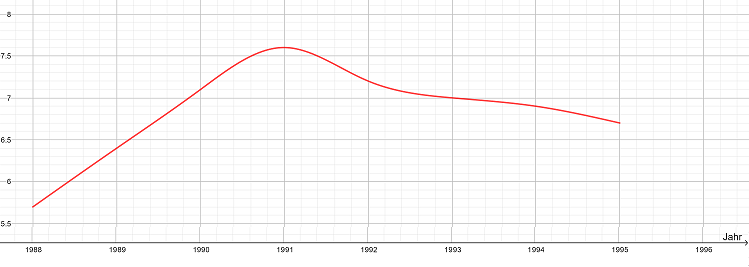
\includegraphics[width=0.8\textwidth]{../Mathematik_1/Bilder/funktionen_verpackungsverbrauch_zeitverlauf_loesung.png} \hspace{0.5cm}
\end{center}
  \begin{itemize}
	  \item[2.]  $1992$
	  \item[3.] Ohne den Gr�nen Punkt h�tte man mit einer j�hrlichen Steigerung um ca $0.5\,\mathrm{Mio}\,\mathrm{t}$ rechnen m�ssen. Die Prognose f�r $1993$ ergibt sich aus dem Verbrauch aus dem Jahr $1991$ plus ca $1.0\, \mathrm{Mio} \, \mathrm{t}$ f�r die Jahre $1992$ und $1993$:  $ 7.6\, \mathrm{Mio}\,\mathrm{t} + 1.0\,\mathrm{Mio}\,\mathrm{t} = 8.6 \,\mathrm{Mio}\,\mathrm{t}$. Die Ersparnis bis zum Jahr $1993$ betr�gt also ca $8.6 \,\mathrm{Mio}\,\mathrm{t} - 7.0\, \mathrm{Mio}\,\mathrm{t} = 1.6 \,\mathrm{Mio}\,\mathrm{t}$, das entspricht einer Einsparung von Verpackung von ca $ \frac{1.6}{8.6} \cdot 100 \% \approx 16\%$.
  \end{itemize}
\end{exercisebox}

\begin{exercisebox}[Mathematische Kurzschreibweise]
	Dr�cken Sie die Aussagen in mathematischer Kurzschreibweise aus.
  \begin{enumerate}
    \item Durch die Funktion $f$ wird der Zahl $3$ die Zahl $10$ zugeordnet.
    \item Die Funktion $g$ nimmt an der Stelle $5$ den Funktionswert $12$ an.
    \item Die Zahl $3$ geh�rt nicht zur Definitionsmenge der Funktion $f$.
    \item Die Funktion $f$ ordnet der Zahl $4$ einen gr��eren Funktionswert zu als der Zahl $5$.
    \item Die Funktionen $f$ und $g$ nehmen f�r $x=2$ denselben Funktionswert an.
    \item Alle Funktionswerte der Funktion $g$ sind positiv.
  \end{enumerate}

	\vspace{0.3cm}
	\noindent\textbf{L�sung:}\newline
  \begin{enumerate}
	  \item $ f(3) =10$
	  \item $g(5) = 12$
    \item $3\not\in D_f$
    \item $f(4) > f(5)$
    \item $f(2) = g(2)$
    \item $W_g\subseteq \mathbb R^+$
  \end{enumerate}
\end{exercisebox}

\begin{exercisebox}[Definitionsbereich]
	Bestimmen Sie den maximalen Definitionsbereich der folgenden Abbildungen:
  \begin{eqnarray*}
          \begin{array}{lll}
        	  (a) \; x\mapsto (x-1)^2 &\quad \quad (b)\; x\mapsto 3-5\cdot x-x^2 & \quad \quad (c)\; x\mapsto \displaystyle{\frac{1}{x}} \\[2ex]
        	  (d) \; x\mapsto \displaystyle{\frac{1}{3-x}} & \quad \quad (e)\; x\mapsto \displaystyle{\frac{1}{(x-1)^2}} &\quad \quad (f) \; x\mapsto \displaystyle{\frac{1}{x^2-1}} \\[2ex]
        	  (g) \; x\mapsto \sqrt{x-3} &\quad \quad (h) \; x\mapsto \displaystyle{\frac{1}{\sqrt{x-3}}} &\quad \quad (i)\; x\mapsto \ln( x +3) 
          \end{array}
  \end{eqnarray*}

	\vspace{0.3cm}
	\noindent\textbf{L�sung:}\newline
  \begin{eqnarray*}
          \begin{array}{lll}
		  (a) \mathbb R &\quad \quad (b)\; \mathbb R & \quad \quad (c)\; \mathbb R\setminus \{0\} \\[2ex]
		  (d) \; \mathbb R\setminus \{3\} & \quad \quad (e)\; \mathbb R \setminus \{ 1\} &\quad \quad (f) \; \mathbb R\setminus \{ -1, 1\} \\[2ex]
		  (g) \; [3,\infty) &\quad \quad (h) \; (3,\infty) &\quad \quad (i)\; (-3,\infty) 
          \end{array}
  \end{eqnarray*}
\end{exercisebox}

\begin{exercisebox}[Bildbereich]
	Bestimmen Sie den Bildbereich (die Bildmenge) der folgenden Abbildungen:
  \begin{eqnarray*}
          \begin{array}{lll}
        	  (a)\; x\mapsto x^2 & \quad \quad (b)\; x\mapsto x^2 +1 & \quad \quad (c)\; x\mapsto 2 - x^2 \\[2ex]
		  (d)\; x\mapsto -(x+2)^2+3 &\quad \quad (e)\; x\mapsto 3\cdot x-0.5 &\quad\quad (f)\; x\mapsto \sin(x) \\[2ex]
    (g)\; x\mapsto 3^x &\quad \quad (h)\; x\mapsto 3 
    \end{array}
  \end{eqnarray*}

	\vspace{0.3cm}
	\noindent\textbf{L�sung:}\newline
  \begin{eqnarray*}
          \begin{array}{lll}
		  (a)\; \mathbb R^+_0 & \quad \quad (b)\; [1,\infty) & \quad \quad (c)\; (-\infty,2] \\[2ex]
		  (d)\; (-\infty,3] &\quad \quad (e)\; \mathbb R &\quad\quad (f)\; [-1,1] \\[2ex]
		  (g)\; \mathbb R^+ &\quad \quad (h)\; \{3\} 
    \end{array}
  \end{eqnarray*}
\end{exercisebox}



%\begin{exercisebox}[Graphen lesen, Maxima, Minima, Symmetrie]
%	\begin{center}
%	\includegraphics[width=0.4\textwidth]{../Mathematik_1/Bilder/Mountainbike.png}
%	\end{center}
%  Eine Mountainbike Tour in dem spanischen El-Ports-Gebirge hat das abgebildete H�henprofil. 
%  \begin{enumerate}
%    \item Wie viele H�henmeter sind beim ersten Anstieg zu �berwinden?
%    \item Wie gro� ist der Gesamtanstieg, der bei der Tour zu �berwinden ist?
%    \item Wie steil ist die letzte Abfahrt ab Streckenkilometer $26$? Geben Sie das Gef�lle in Prozent und den Steigungswinkel an.
%    \item Zur Quelle Canaleta f�hrt nur eine Sackgasse. Wie �u�ert sich das im Graphen? Wie lang ist vermutliche diese Sackgasse?
%    \item Wo kann es noch eine Weitere Sackgasse geben?
%  \end{enumerate}
%
%%  \begin{tabular}{c|c}
%%    Kilometer & H�henmeter \\
%%    $0$ & $550$\\
%%    $1$ & $700$\\
%%    $4$ & $800$\\
%%    $5$ & $630$\\
%%    $6$ & $\ldots$
%%  \end{tabular}
% Lampbacher Schweitzer, p. 12
%\end{exercisebox} 
 \newpage 
\setcounter{exercise}{0}\pagestyle{empty} 
\section*{Eigenschaften von Funktionen L�sungen}\label{MA1-eigenschaften-von-funktionen-loesungen}

\ifintegriereaufgaben
	Regeln und Beispiele, die zum Verst�ndnis der L�sungswege hilfreich sind, finden Sie im Skript\wennreferenzvorhanden{MA1-eigenschaften-von-funktionen}{ (Abschnitt \abschnittsverweis{MA1-eigenschaften-von-funktionen})}.
\else 
	Regeln und Beispiele, die zum Verst�ndnis der L�sungswege hilfreich sind, finden Sie im Skript.
\fi 

\begin{exercisebox}[Symmetrie]
  Welche der folgenden Funktionen ist gerade, welche ungerade?
  \begin{eqnarray*} \begin{array}{lll} 
		  (a)\; x\mapsto -2\cdot x^6 + 3\cdot x^2  \quad& (b)\quad x\mapsto 2-3\cdot x^4  \quad & (c)\; x\mapsto 2-3\cdot x^3 \\[1ex]
		  (d)\; x\mapsto 3\cdot x^3-x+1 \quad & (e)\; x\mapsto x\cdot (2\cdot x^2 - \frac13 \cdot x^4) \quad & (f)\; x\mapsto (x-1)\cdot(x-2) \\[1ex]
		  (g)\; x\mapsto (x-1)^3+3\cdot x^2+1 \quad &(h)\; x\mapsto (1-3\cdot x^2)^2 & (i)\; x\mapsto (x-x^2)^2 
	  \end{array}
  \end{eqnarray*}
 

  \hspace{0.3cm}
  \newline
  \textbf{L�sung:}
  \begin{center}
	  \begin{tabular}{c|c|c|c|c|c|c|c|c|c}
	  & $a)$ & $b)$ & $c)$ & $d)$ & $e)$ & $f)$ & $g)$ & $h)$ & $i)$ \\
	  \hline
	  \hline
	  gerade & $\bullet$ & $\bullet$ &  &  &  &  &  & $\bullet$ & \\
	  \hline
	  ungerade &  &  &  &  & $\bullet$ &  &  $\bullet^{(*)}$&  &  \\
	  \hline
	  weder noch &  &  & $\bullet$ & $\bullet$ & & $\bullet$ &  & & $\bullet$ 
  \end{tabular}
  \end{center}
  $(*)$ $(x-1)^3+3\cdot x^2+1  = (x-1)\cdot (x^2-2\cdot x+1) = x^3-2\cdot x^2+x^2 - x^2 +2\cdot x^2 -1  +3\cdot x^2+1  = x^3 -2\cdot x$
\end{exercisebox}

\begin{exercisebox}[Umkehrfunktion] %Andreas
Gegeben sei die (diskrete) Funktion $f:\{1,2,3,4\} \to \mathbb N$ mit der Wertetabelle 
\begin{center}
\begin{tabular}{l|l|l|l|l}
$x$ & $1$ & $2$ & $3$ & $4$ \\ 
\hline
$f(x)$ & $9$ & $6$ & $7$ & $8$
\end{tabular}
\end{center}

	\vspace{0.3cm}
	\noindent\textbf{L�sung:}\newline
Die Umkehrfunktion $f^{-1}:\{6,7,8,9\} \to \{1,2,3,4\}$ besitzt die folgende Wertetabelle 
\begin{center}
\begin{tabular}{l|l|l|l|l}
$x$ & $9$ & $6$ & $7$ & $8$ \\
\hline
$f^{-1}(x)$ & $1$ & $2$ & $3$ & $4$ 
\end{tabular}
\end{center}
\end{exercisebox}

\begin{exercisebox}[Umkehrfunktion] 
  Auf welchen Intervallen ist $f$ umkehrbar? Bestimmen Sie $f^{-1}$ und geben Sie $D_{f^{-1}}$ an
  \begin{eqnarray*}
	  \begin{array}{lll} (a)\; f: x \mapsto 4x-x^2  & \quad \quad (b)\; f:x \mapsto \displaystyle{\frac{2\cdot x}{x-1}} & \quad \quad (c)\; f:x\mapsto x\cdot |x| \end{array}
  \end{eqnarray*}

	\vspace{0.3cm}
	\noindent\textbf{L�sung:}\newline
	\begin{itemize}
		\item[(a)] Offenbar gilt \[f: \mathbb R \to (-\infty, 4], x\mapsto x\cdot ( 4-x)\] $f$ besitzt dasselbe asymptotische Verhalten wie \(x\mapsto -x^2\) und ist demnach auf \(\mathbb R\) nicht injektiv und damit nicht invertierbar. Aber man kann \(f\) auf zwei Intervalle einschr�nken, auf denen Injektivit�t sicher gestellt ist, n�mlich auf dem Intervall $I_1:= (-\infty,2]$ und auf dem Intervall $I_2:=[2,\infty)$. Die Abbildungsvorschriften der entsprechenden Umkehrfunktionen erh�lt man, in dem man die Gleichung \(y=4\cdot x-x^2\) nach \(x\) aufl�st: 
\begin{equation*}
	\begin{array}{rr rcl l}
		\forall x\geq 2: && y &=& 4\cdot x-x^2 &  \\
		&\Leftrightarrow &y &=& \left( -x^2+4\cdot x \color{red}{-4} \right) \color{red}{+ 4} & \\
		&\Leftrightarrow &y &=& -(x-2)^2 + 4 & || - 4 \\
		&\Leftrightarrow &4-y &=& (x-2)^2 & || \sqrt{\cdot} \\[2ex]
		&\stackrel{ x\geq2 !}{\Leftrightarrow} &\sqrt{4-y} &=& x-2 & || +2 \\
		&\Leftrightarrow &\pm\sqrt{4-y}+2 &=& x & 
	\end{array}
  \end{equation*}
  Entsprechend l�st man f�r \(x<2\) auf und erh�lt:
  \begin{eqnarray*}
	  \begin{array}{l l l}
  f_1^{-1}: &(-\infty, 4] \to (-\infty, 2], &\; x\mapsto 2-\sqrt{4-x} \\  
  f_2^{-1}: &(-\infty, 4] \to  [2, \infty),&\; x\mapsto 2+\sqrt{4-x}  \\
  \end{array}
  \end{eqnarray*}
  \item[(b)] $f$ ist auf $\mathbb R\setminus\{1\}$ invertierbar und es gilt:
	  \begin{eqnarray*}
  f^{-1}: \mathbb R\setminus\{1\} \to \mathbb R\setminus\{ 1\}, \, x\mapsto \frac{x}{x-2}  
  \end{eqnarray*}
  \item[(c)] Um die Abbildung \(f\) zu verstehen, l�sen wir den Betragsstrich auf: 
	  \begin{equation*}
		  f(x) = \begin{cases} x^2, \; x\geq0\,,\\ -x^2, \; x<0\,.\end{cases}
	  \end{equation*}
	  \(f\) ist eine auf ganz \(\mathbb R\) definierte streng monoton steigende Funktion (f�r \(x\geq 0\) entspricht sie der Normalparabel und f�r \(x<0\) der, an der \(x\)-Achse gespiegelten Normalparabel). Also $f$ ist auf $\mathbb R$ invertierbar und wir bestimmen die Abbildungsvorschrift der Umkehrfunktion st�ckweise wie folgt: 
	  \begin{eqnarray*}
		  x\geq 0 \Rightarrow y\geq 0: \quad y = x^2 \Rightarrow +\sqrt{y} = x\,.\\
		  x< 0 \Rightarrow y<0: \quad y = -x^2 \Leftrightarrow |y| = x^2 \Leftrightarrow -\sqrt{|y|} = x\,.
	  \end{eqnarray*}
	  Nach der Variablenumbennenung erhalten wir insgesamt
	  \begin{eqnarray*}
  f^{-1}: \mathbb R \to \mathbb R, x\mapsto \begin{cases} \sqrt{x}, &x\geq 0 \\ -\sqrt{|x|}, &x<0 \end{cases} 
  \end{eqnarray*}
  \end{itemize}
\end{exercisebox}


\begin{exercisebox}[Anwendung: Verpackungsreduktion] %LS p.37
Umweltbewusste Studenten behaupten: Bei Dosen-Limo ist die Verpackung teurer als der Inhalt. F�r die �berpr�fung treffen die Studenten folgende Annahmen: Die Dose ist ein Zylinder, dessen H�he doppelt so gro� ist wie sein Durchmesser. F�r den Hersteller kostet $1$ Liter Limo $15\,\mathrm{ct}$. Die Kosten f�r $1\,\mathrm{dm}^2$ Blech betragen $3 \,\mathrm{ct}$
  \begin{itemize}
	  \item[(a)] �berpr�fen Sie die Behauptung f�r den Dosenradius $r=3 \,\mathrm{cm}$.
	  \item[(b)] Ab welchem Dosenradius ist der Inhalt teurer als die Dose?
  \end{itemize}

	\vspace{0.3cm}
	\noindent\textbf{L�sung:}\newline
	\begin{enumerate}
		\item Die Behauptung trifft zu!  Mit $h=4r [\mathrm{dm}]$ erh�lt man 
			\begin{center}
	\begin{tabular}{l|l|l}
		& Funktionaler Zusammenhang & Einheit \\[1ex]
		\hline
		Materialbedarf $M$ & $\displaystyle{M: r\mapsto 2 \cdot(\pi\cdot r^2) + (2\pi \cdot r)\cdot h =  10\pi \cdot r^2}$  &$ [\mathrm{dm}^2]$\\[1ex]
		Doseninhalt $V$ & $\displaystyle{V: r\mapsto (\pi\cdot r^2)\cdot h=4\pi \cdot r^3 }$  &$[\mathrm{dm}^3] = [\mathrm{l}]$\\[1ex]
		Materialkosten $K_M$ & $\displaystyle{K_M: r\mapsto 3 \cdot M(r) = 30\pi \cdot r^2 }$ &$[\mathrm{ct}] $\\[1ex]
		Kosten f�r Limo $K_L$ & $\displaystyle{K_L: r\mapsto 15 \cdot V(r) = 60\pi \cdot r^3 }$ &$[\mathrm{ct}] $
	\end{tabular}
\end{center}
Und f�r $r = 3 \,\mathrm{cm} = 0.3\, \mathrm{dm}$ folgt
	\begin{center}
	\begin{tabular}{l|l}
		Materialkosten & $\displaystyle{K_M(0.3\, \mathrm{dm} ) = 2.7\pi \approx 8.48 \,\mathrm{ct} }$ \\
		Kosten f�r Limo & $\displaystyle{K_L(0.3 \, \mathrm{dm}) = 1.62\pi \approx 5.09 \, \mathrm{ct} }$ \\
	\end{tabular}
\end{center}
\item  Die Bedingung $K_L(r) > K_M(r)$ wird f�r $r>\frac12 \mathrm{dm}$ erf�llt.
	\end{enumerate}
\end{exercisebox}

\begin{exercisebox}[Anwendung: Kostenreduktion] %LS p.38
	Die Herstellungskosten eines Airbus-Seitenleitwerks aus Metall werden angen�hert durch \[ k_1: x\mapsto \frac{20\cdot x+5000}{x+50}\,,\] wobei $x$ die Anzahl der hergestellten Leitwerke und $k_1(x)$ eine willk�rliche Geldeinheit beschreibt. Nachdem $300$ Leitwerke hergestellt sind, wird erwogen, die Produktion auf Kunststoffleitwerke umzustellen. Die St�ckkosten betragen dann n�herungsweise \[k_2:x\mapsto \frac{15\cdot x-2500}{x-250}\,, \quad x>300\,.\]
  \begin{enumerate}
 \item Zeichnen Sie die beiden Graphen, zum Beispiel mit Hilfe von Geogebra o.�..
    \item Wie verhalten sich die St�ckkosten bei sehr gro�en Produktionszahlen?
    \item Ab welcher St�ckzahl ist das Kunststoffleitwerk billiger?
  \end{enumerate}

	\vspace{0.3cm}
	\noindent\textbf{L�sung:}\newline
	\begin{center}
	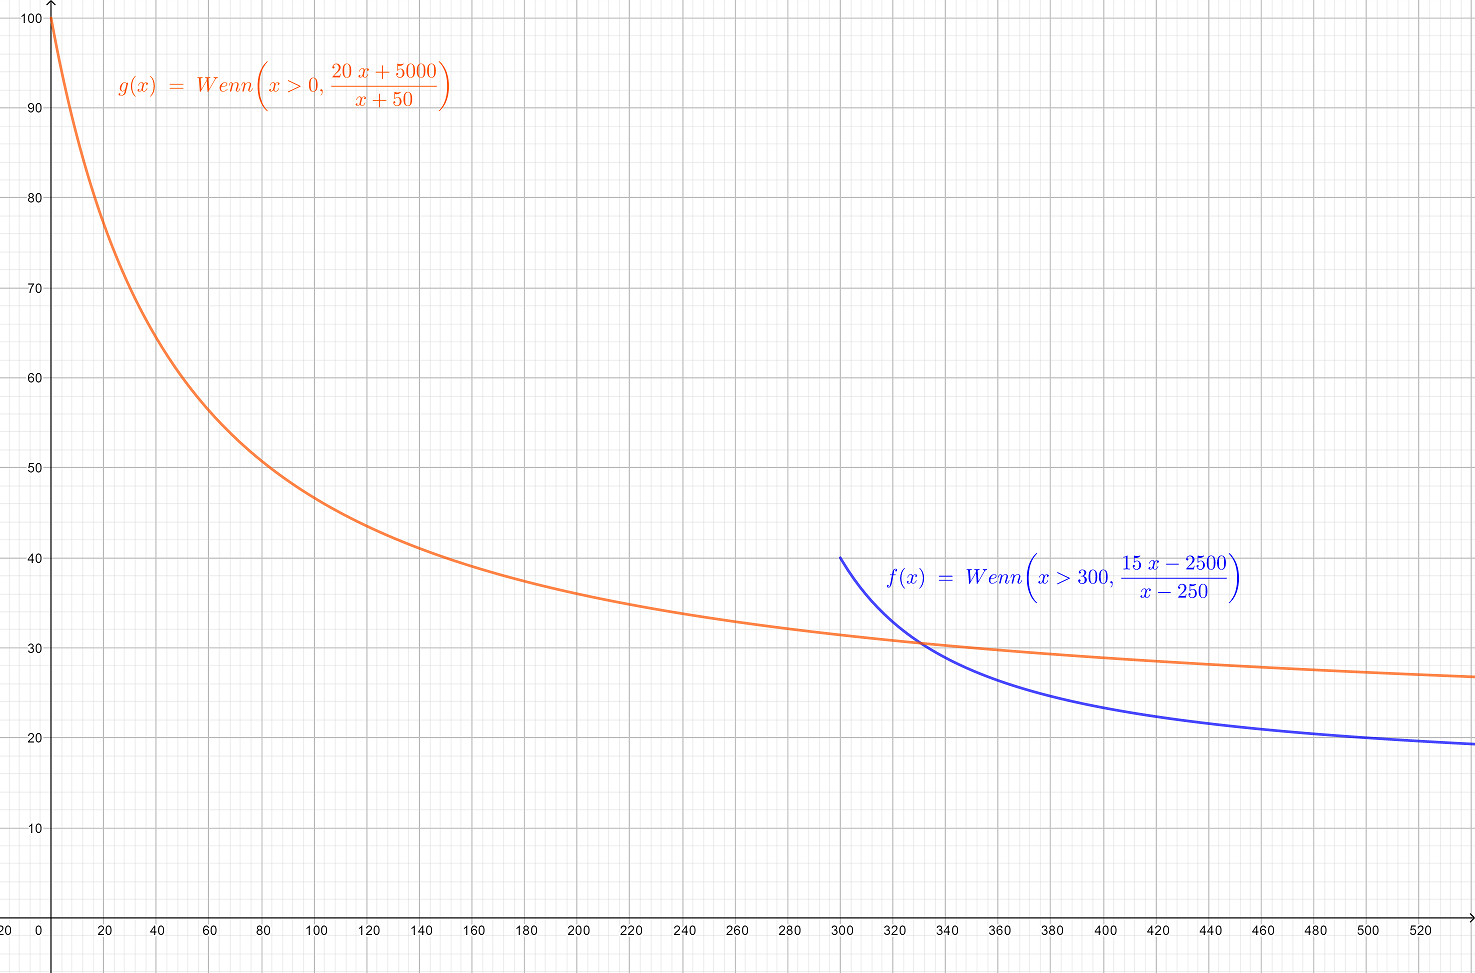
\includegraphics[width=0.9\textwidth]{../Mathematik_1/Bilder/rationale_funktionen_stueckkosten_leitwerke_loesung.png}
	\end{center}
	\begin{itemize}
	\item[2.] $\displaystyle{\lim\limits_{x\to\infty} k(x) = 20}$ und $\displaystyle{\lim\limits_{x\to\infty} k^*(x) = 15}$ und 
	\item[3.] $k^*(x) < k(x) $ f�r $x>330$.
  \end{itemize}
	
\end{exercisebox}
 \newpage 
\setcounter{exercise}{0}\pagestyle{empty} \section*{Lineare Funktionen L�sungen}\label{MA1-lineare-funktionen-loesungen}

\ifintegriereaufgaben
	Regeln und Beispiele, die zum Verst�ndnis der L�sungswege hilfreich sind, finden Sie im Skript\wennreferenzvorhanden{MA1-lineare-funktionen}{ (Abschnitt \abschnittsverweis{MA1-lineare-funktionen})}.
\else
	Regeln und Beispiele, die zum Verst�ndnis der L�sungswege hilfreich sind, finden Sie im Skript.
\fi 

\begin{exercisebox}[Abbildungsvorschrift] %Andreas
	Bestimmen Sie die Funktionsgleichung in der Form \[ f(x) = m\cdot x + b\] einer linearen Funktion durch die Punkte \( (1,5| 2)\) und \( (-3|3)\).

	\vspace{0.3cm}
	\noindent\textbf{L�sung:}\newline
	Es gilt \[ y(x) = \frac{3-2}{-3-1,5}(x-1,5)+2=-\frac29\left( x-\frac32\right) +2 = -\frac29 x + \frac73\,.\]
\end{exercisebox}

\begin{exercisebox}[Umkehrfunktion]
	F�r welche reellen Werte von \(m\) und \(b\) ist die lineare Funktion $f: x\mapsto m\cdot x+b$ umkehrbar? 

	\vspace{0.3cm}
	\noindent\textbf{L�sung:} Alle linearen Funktionen mit $m\not=0$ sind umkehrbar.
\end{exercisebox}

\begin{exercisebox}[Abbildungsvorschrift] %Lovis
	Die durch die Gleichung \( x +3y= 8\) beschriebene Gerade im \(\mathbb R^2\) wird um zwei Einheiten nach rechts und um eine Einheit nach oben geschoben. Geben Sie die Abbildungsvorschrift f�r die verschobene Gerade an.  

	\vspace{0.3cm}
	\noindent\textbf{L�sung:}\newline
	$y(x) = \frac13(8-x) \Rightarrow \tilde y(x) = y(x-2) +1 = \frac13(10-x) +1$  
	\begin{center}
	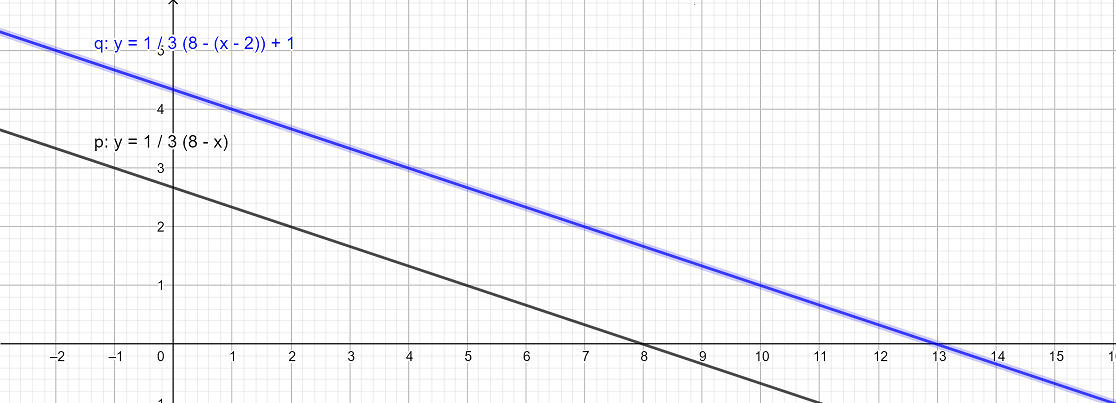
\includegraphics[width=0.8\textwidth]{../Mathematik_1/Bilder/lineare_funktionen_geradenverschiebung_loesung.png}
	\end{center}
\end{exercisebox}

\begin{exercisebox}[Betragsfunktion] %Lovis
Skizzieren Sie die Menge \( \{ (x,y) \in \mathbb R^2: y<1+|x|\}\). Kennzeichnen Sie, ob die R�nder dazu geh�ren oder nicht. 

	\vspace{0.3cm}
	\noindent\textbf{L�sung:}\newline
	\begin{center}
	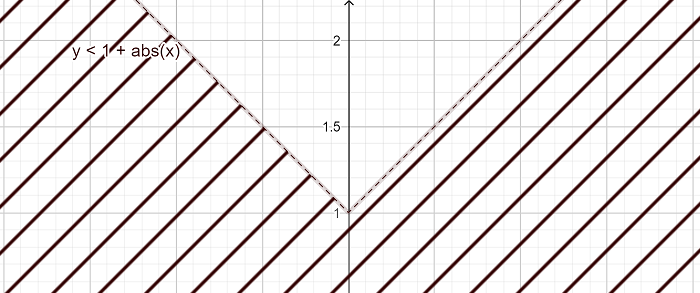
\includegraphics[width=0.8\textwidth]{../Mathematik_1/Bilder/ungleichungen_betragsfunktion_untergraph_loesung.png}
\end{center}
\end{exercisebox}

\begin{exercisebox}[Betragsfunktion] %LS p.21
		Stellen Sie die gegebenen Funktionen ohne Betragszeichen dar und zeichnen Sie den Graph:
  \begin{eqnarray*}
	  \begin{array}{llll}
		  (a)\; f:x \mapsto 2\cdot |x| & \quad (b)\; f:x \mapsto |2-x| & \quad (c)\; f:x \mapsto |2+x| &\quad (d)\; f:x \mapsto x-|x|
	  \end{array}
  \end{eqnarray*}

	\vspace{0.3cm}
	\noindent\textbf{L�sung:}\newline
  \begin{eqnarray*}
	  \begin{array}{lll}
		  (a)\; f:x \mapsto \begin{cases} 2x, &\; x\geq 0 \\ -2x, &\; x<0 \end{cases} & \; (b)\; f:x \mapsto \begin{cases} x-2, &x\geq 2 \\ 2-x, & x<2 \end{cases} & \; (c)\; f:x \mapsto\begin{cases} 2+x, &x\geq -2 \\ -2-x, &x<-2\end{cases} \\
		  (d)\; f:x \mapsto \begin{cases} 0, & x\geq 0 \\ 2x, &x<0 \end{cases}
	  \end{array}
  \end{eqnarray*}
  \begin{center}
	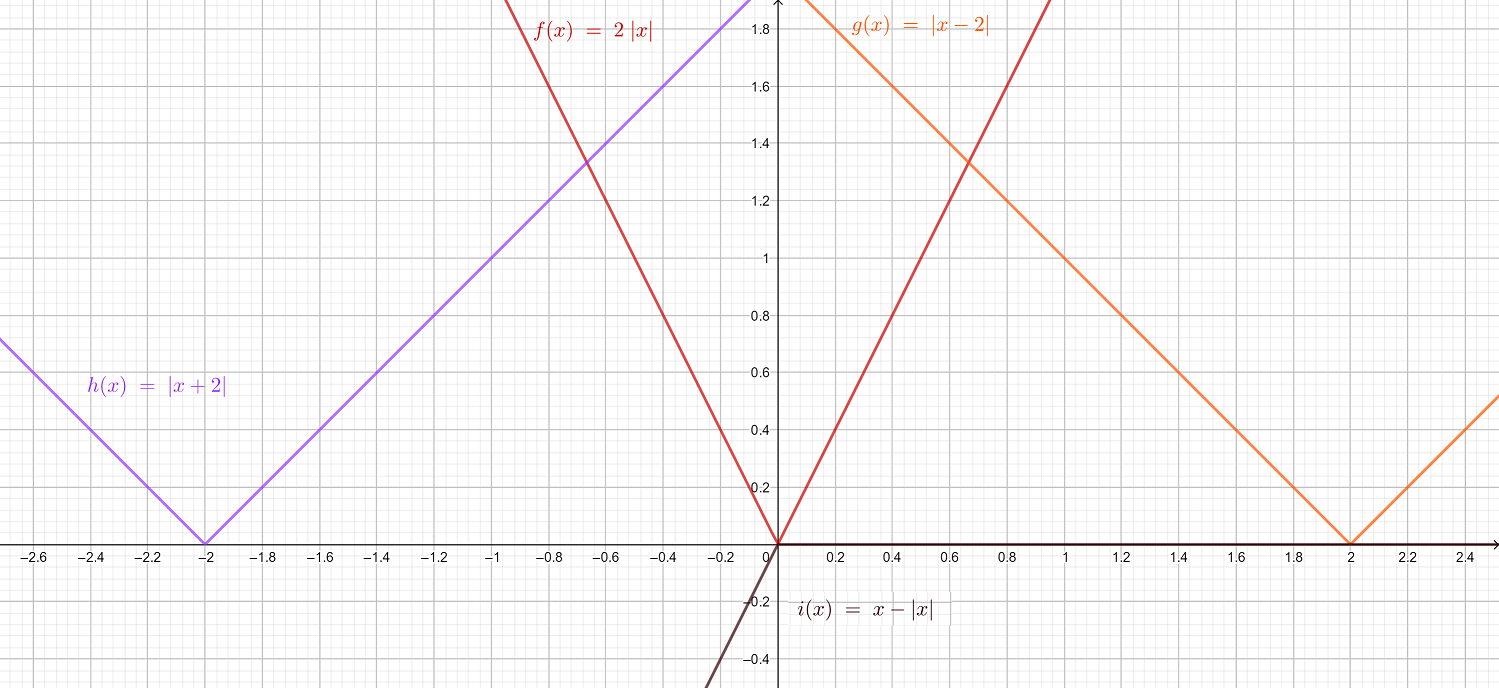
\includegraphics[width=0.9\textwidth]{../Mathematik_1/Bilder/betragsfunktionen_graphenvergleich_loesung.png}
\end{center}
\end{exercisebox}

\begin{exercisebox}[Anwendung: Interpolation] %Andreas
	Gegeben sind die Messpunkte $(x_i,y_i), \; i= 0,1,2,3,$ mit $(-1,5| 2),(-0,25| 3,5),(0,5| 3,3),(1,2| 2,8)$. Bestimmen Sie den linearen Spline und werten Sie ihn am Punkt $x= 0,2$ aus. Welchen Wert erhalten Sie?

	\vspace{0.3cm}
	\noindent\textbf{L�sung:}\newline
	Wegen $0,2\in [-0,25;0.5]$ gilt  \[ s(0,2) = \frac{3,3-3,5}{0,5 - (-0,25)}(0,2-(-0,25))+3,5=3,38\,.\]
\end{exercisebox}

\begin{exercisebox}[Anwendung: Ausgleichsgerade] %Lucy
	Gegeben sind die Messpunkte $(x_i,y_i), \; i= 0,1,2,3,$ mit $(-1,5| 2),(-0,25| 3,5),(0,5| 3,3),(1,2| 2,8)$.	

	\vspace{0.3cm}
	\noindent\textbf{L�sung:}\newline
	\begin{eqnarray*} 
		r(x) = \frac{2048}{6403}\,x+\frac{185943}{64030} \approx 0{,}31985\,x+2{,}90400 \quad\Rightarrow\quad r(0{,}2)\approx 2{,}96797\,.
	\end{eqnarray*}
	\centering
	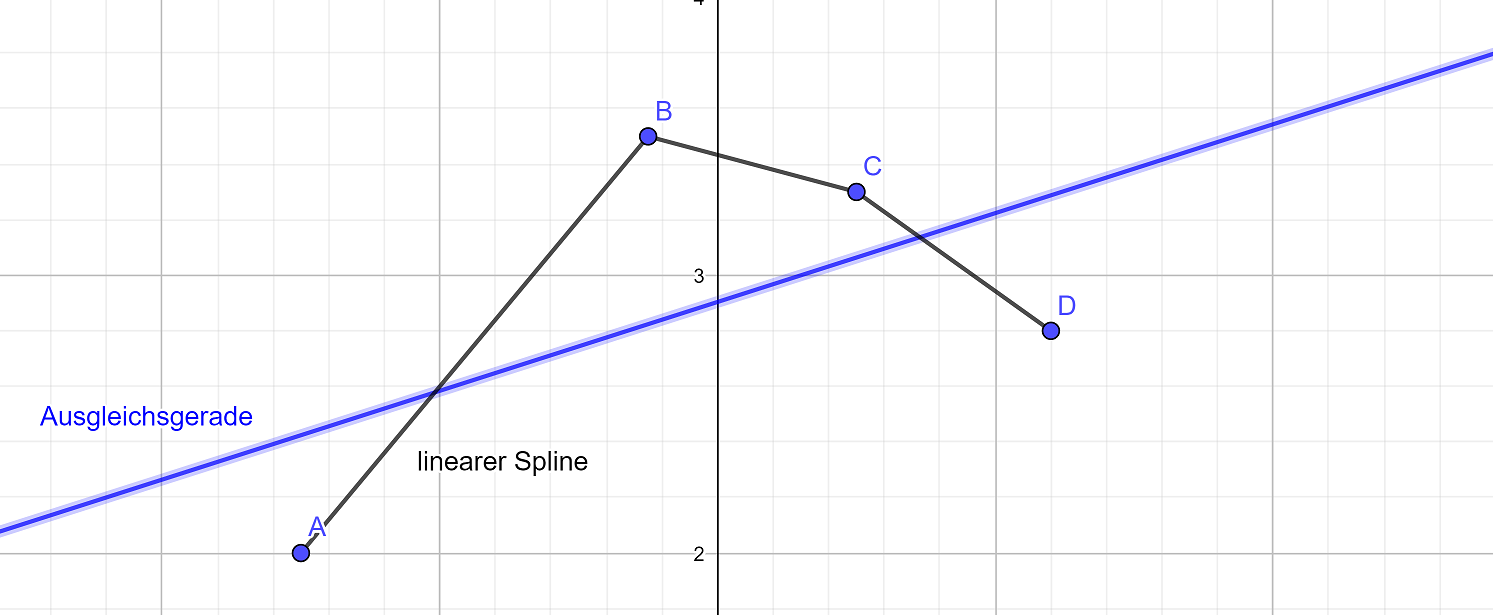
\includegraphics[width=0.9\textwidth]{../Mathematik_1/Bilder/interpolation_linearer_spline_ausgleichsgerade_loesung.png}
\end{exercisebox}

\begin{exercisebox}[Anwendung: Dimensionierung Solarzellen] %LS p.21
	Sonnenkollektoren wandeln Lichtenergie in W�rme um, die an den Warmwasserspeicher abgef�hrt wird. Die ben�tigte Kollektorfl�che h�ngt linear vom Volumen des Speichers ab. Bei einer Speichertemperatur von $45^\circ \mathrm{C}$ wird f�r $200$ Liter eine Kollektorfl�che von $3\mathrm{m}^2$ und f�r $500$ Liter eine Kollektorfl�che von $7\mathrm{m}^2$ empfohlen. Pro Person wird mit einem Verbrauch von $50$ Liter Warmwasser am Tag gerechnet. Das Speichervolumen sollte $50\%$ �ber dem Verbrauch liegen. 
  \begin{enumerate}
    \item Bestimmen Sie die Funktion, die der Personenanzahl die Kollektorfl�che zuordnet.
    \item Wie gro� sollte die Kollektorfl�che bei einem $4$-Personen Haushalt sein?
    \item F�r wie viele Personen reicht eine Kollektorfl�che von $8\mathrm{m}^2$?
  \end{enumerate}

	\vspace{0.3cm}
	\noindent\textbf{L�sung:}\newline
	Wir m�ssen die Informationen aus der Textaufgabe in mathematische Formeln gie�en und das machen wir jetzt - St�ck f�r St�ck: 
	\begin{itemize}
		\item Das gew�nschte Speichervolumen \(V\) h�ngt von der Personenanzahl \(x\) ab und zwar soll gelten, dass pro Person ein Speichervolumen von \(50\) Litern (effektiver Verbrauch) plus \(25\) Litern (Puffer) ben�tigt wird, also \[ s: x\mapsto 75\cdot x\,.\] 
		\item Die Kollektorfl�che h�ngt \textbf{linear} vom Speichervolumen ab. Mit den angegebenen Informationen, n�mlich \(P_1\left( 200 [\mathrm l], 3 [\mathrm{m}^2]\right)\) und  \(P_2\left( 500 [\mathrm l], 7 [\mathrm{m}^2]\right)\) l��t sich die lineare Funktion berechnen (Zwei-Punkte-Formel): \[ K: V\mapsto \dfrac{3-7}{200 - 500} \left[ \dfrac{\mathrm{l}}{\mathrm{m^2}}\right]\left( V-500\right) [\mathrm m^2] + 7 [\mathrm{l}] = \frac{1}{75}V + \frac13\,.\]
		\item Um nun die Kollektorfl�che in Abh�ngigkeit der Personenanzahl anzugeben, m�ssen die ermittelten Abbildungen hintereinander ausgef�hrt werden und das ergibt die unter \(1.\) gesuchte Funktion.\footnote{Diese Hintereinanderausf�hrung hei�t Verkettung von Funktionen\wennreferenzvorhanden{MA1-verkettung-von-funktionen}{ (Abschnitt \abschnittsverweis{MA1-verkettung-von-funktionen})}, also \(f = K \circ s\).}: Personenanzahl \(x\) \(\mapsto\) Speichervolumen \(V\) \(\mapsto\) Kollektoroberfl�che \(K\), also \[f(x) = K\left(s(x)\right) = \dfrac{1}{75}\left( 75 \cdot x\right) + \dfrac13 = x + \dfrac13\,.\]
	\end{itemize}
	Nun zur L�sung der einzelnen Fragen:
	\begin{itemize}
\item[1.] \( f: x\mapsto x + \dfrac13\). 
	  \item[2.] $f(4)=4 + \frac13 \; \Rightarrow $ Kollektorfl�che ist $4, \bar 3 [\mathrm{m}^2]$.
	  \item[3.] $f(x) = 8 \; \Rightarrow $ $7$-Personen-Haushalt.
  \end{itemize}
\end{exercisebox}

 \newpage 
\setcounter{exercise}{0}\pagestyle{empty} \section*{Potenz- und Wurzelfunktionen L�sungen}\label{MA1-potenz-und-wurzelfunktionen-loesungen}

\ifintegriereaufgaben
	Regeln und Beispiele, die zum Verst�ndnis der L�sungswege hilfreich sind, finden Sie im Skript\wennreferenzvorhanden{MA1-potenz-und-wurzelfunktionen}{ (Abschnitt \abschnittsverweis{MA1-potenz-und-wurzelfunktionen})}.
\else
	Regeln und Beispiele, die zum Verst�ndnis der L�sungswege hilfreich sind, finden Sie im Skript.
\fi 

\begin{exercisebox}[$f:x\mapsto  3\cdot \sqrt{4-x^2}$]
  Gegeben ist die Funktion $f:x\mapsto  3\sqrt{4-x^2}$.
  \begin{itemize}
	  \item[(a)] Geben Sie die Funktionswerte an den Stellen $-1$ und $\sqrt{3}$ an.
    \item[(b)] Berechnen Sie $f(0)$, $f(2)$, und $f(\frac23)$.
    \item[(c)] Bestimmen Sie die maximale Definitionsmenge und die Wertemenge von $f$.
    \item[(d)] Pr�fen Sie rechnerisch, ob der Punkt $P(-\sqrt 2| 3\sqrt 2)$ auf dem Graphen von $f$ liegt.
  \end{itemize}

	\vspace{0.3cm}
	\noindent\textbf{L�sung:}\newline
  \begin{itemize}
	  \item[(a)] $f(-1) = 3 \sqrt{3}$, $f(\sqrt{3}) = 3$
	  \item[(b)] $f(0) = 6, \, f(2) = 0, \, f(3/2) = 3/2 \sqrt{7}$ 
	  \item[(c)] $ 4-x^2 \stackrel{!}{\geq} 0 \Rightarrow D_f=[-2,2]$.
	  \item[(d)] $f(-\sqrt{2}) = 3\cdot \sqrt{4-2} = 3\cdot \sqrt{2} \; \Rightarrow$ $P$ liegt auf dem Graphen von $f$ liegt.
  \end{itemize}
\end{exercisebox}

\begin{exercisebox}[Symmetrie]
	Bestimmen Sie das Symmetrieverhalten der folgenden Funktionen in ihrem maximalen Definitionsbereich
  \begin{eqnarray*}
	  \begin{array}{lll} 
		  (a)\, f:x\mapsto 4\cdot x^2-16 &\quad (b) f:x\mapsto \displaystyle{\frac{x^3}{x^2+1}} &\quad (c)\; f:x\mapsto |x^2-4|\\ (d)\; f:x\mapsto \displaystyle{\frac{x^2-1}{1+x^2}} &\quad (e)\, f:x\mapsto \sqrt{x^2-25} &\quad (f)\,f:x\mapsto \displaystyle{\frac{1}{x-1}}
	  \end{array}
  \end{eqnarray*}

 \hspace{0.3cm}
\noindent \textbf{L�sung:}\newline
  \begin{itemize}
	  \item[(a)] $y(-x)=4\cdot (-x)^2-16 = y(x)$, d.h. gerade
	  \item[(b)] $y(-x)=\frac{(-x)^3}{(-x)^2+1} = -y(x)$, d.h. ungerade
	  \item[(c)] $y(-x)=|(-x)^2-4|=y(x)$, d.h. gerade
	  \item[(d)] $y(-x)=\frac{(x-)^2-1}{1+(-x)^2} = y(x)$, d.h. gerade
	  \item[(e)] $y(-x)=\sqrt{ (-x)^2-25} = y(x)$, d.h. gerade
	  \item[(f)] $y(-x)=\frac{1}{-x-1}$ und damit $y(-x)\not= y(x) \land y(x)\not= -y(x) $, d.h. weder gerade noch ungerade
  \end{itemize}
\end{exercisebox}

\begin{exercisebox}[Monotonie]
	Untersuchen Sie die folgenden Funktionen auf Monotonie
  \begin{eqnarray*}
	  \begin{array}{llll} 
		  (a)\, f:x\mapsto x^4 &\quad (b)\; f:x\mapsto \displaystyle{\sqrt{x-1}} &\quad (c)\; f:x\mapsto x^3+2\cdot x \quad (d)\; f:x\mapsto \displaystyle{| x^2-2\cdot x+1|} 
	  \end{array}
  \end{eqnarray*}

 \hspace{0.3cm}
\noindent\textbf{L�sung:}\newline
  \begin{itemize}
	  \item[(a)] streng monoton fallend auf $(-\infty, 0]$ und streng monoton steigend auf $[0,\infty)$
	  \item[(b)] streng monoton steigend: die Wurzelfunktion $\sqrt{x}$ ist auf $\mathbb R^+_0$ streng monoton steigend, da aus $x_1 <x_2$ folgt, dass $(\sqrt{x_1})^2 < (\sqrt{x_2})^2$. Da beide Argumente nichtnegativ sind und die Funktion $x\mapsto x^2$ auf $\mathbb R^+_0$ streng monoton steigend ist, folgt damit auch $\sqrt{x_1} < \sqrt{x_2}$. Setzt man $x_1= 1+h_1$ und $x_2=1+h_2$ mit $0\leq h_1 <h_2$ ein, so folgt hiermit $\sqrt{x_1-1} = \sqrt{1+h_1-1} = \sqrt{h_1} < \sqrt{h_2} = \sqrt{x_2+1}$ und damit die Behauptung.
	  \item[(c)] Sowohl $y_1(x) =x^3$ als auch $y_2(x) = x$ sind streng monoton wachsend auf $\mathbb R$. Da aus $x_1<x_2$ auch $y_1(x_1) + 2\cdot y_2(x_1) < y_1(x_2) + 2\cdot y_2(x_2)$ folgt (Addieren Sie hier zwei Ungleichungen mit demselben Ungleichheitszeichen), dass die Funktion auf ganz $\mathbb R$ streng monoton w�chst.
	  \item[(d)] Es gilt $y(x) = |(x-1)^2|=(x-1)^2$, da Quadrate immer nichtnegativ sind. Das bedeutet, dass die Funktion eine um eine Stelle nach rechts verschobene Normalparabel ist. Damit ist sie auf $(-\infty, 1]$ streng monoton fallend und auf $[1,\infty)$ streng monoton steigend.
  \end{itemize}
\end{exercisebox}

\begin{exercisebox}[Umkehrfunktion]
  \begin{itemize}
	  \item[(a)] Welche der Potenzfunktionen $f$ mit $f(x) = x^n,\; n\in\mathbb N\setminus\{0\}$  sind umkehrbar?
	  \item[(b)] Wie lauten die Umkehrfunktionen von folgenden Funktionen? \[ (a) \; f:x\mapsto \frac{1}{2\cdot x}\quad \quad (b)\; g:x\mapsto \sqrt{3\cdot x}\]
  \end{itemize}

 \hspace{0.3cm}
\noindent\textbf{L�sung:}\newline
  \begin{itemize}
	  \item[(a)] Potenzfunktionen mit ungeradem Exponenten $n$ sind umkehrbar auf $\mathbb R$.
	  \item[(b)] $(a) \; f^{-1}: \mathbb R\setminus\{0\} \to \mathbb R\setminus\{0\}, \; x\mapsto \displaystyle{\frac{1}{2\cdot x}} \quad\quad (b)\; g^{-1}: [0,\infty) \to [0,\infty), \; x\mapsto \displaystyle{\frac{x^2}{3}}$
		  \end{itemize}
\end{exercisebox}

\begin{exercisebox}[Gleichungen]
	L�sen Sie folgende Gleichungen
  \begin{eqnarray*}
	  \begin{array}{llll} 
		  (a)\, \sqrt{ -3 +2\cdot x} = 2 &\quad (b)\; \sqrt{x^2+4} -x = -2 &\quad (c)\; \sqrt{x-1} = \sqrt{x+1}\quad& (d)\; \sqrt{2\cdot x^2-1}+x=0 
	  \end{array}
  \end{eqnarray*}

 \hspace{0.3cm}
\noindent\textbf{L�sung:}\newline
  \begin{itemize}
	  \item[(a)] 
		  \begin{eqnarray*}
			  \begin{array}{c r c l l }
				  & \sqrt{-3+2\cdot x} &=& 2 & |(\cdot)^2 \\
				  \Rightarrow & -3+2\cdot x &=& 4 &|+3 \\
				  \Leftrightarrow & 2\cdot x &=& 7 &| :2 \\
				  \Leftrightarrow & x &=& 7/2 
			  \end{array}
		  \end{eqnarray*}
		  Die Probe ergibt $\sqrt{-3+2\cdot 7/2}=2$ eine wahre Aussgae. Also ist $\mathbb L=\{7/2\}$.
	  \item[(b)] 
		  \begin{eqnarray*}
			  \begin{array}{c r c l l }
				  &\sqrt{x^2+4}-x &=& -2& | +x \\
				  \Leftrightarrow &\sqrt{x^2+4} &=& x-2& | (\cdot)^2 \\
				  \Rightarrow & x^2+4 &=& x^2-4\cdot x+4 &|-x^2-4 \\
				  \Leftrightarrow & 0 &=& -4\cdot x & |:(-4) \\
				  \Leftrightarrow & x&=& 0 
			  \end{array}
		  \end{eqnarray*}
		  Die Probe ergibt $\sqrt{0^2+4} = 0-2$ eine falsche Aussage. Also ist $\mathbb L=\emptyset$.
	  \item[(c)] 
		  \begin{eqnarray*}
			  \begin{array}{c r c l l }
				  &\sqrt{x-1} &=& \sqrt{x+1} |(\cdot)^2 \\
				  \Rightarrow & x-1 &=& x+1 & |-x \\
				  \Leftrightarrow & -1 &=& 1 
			  \end{array}
		  \end{eqnarray*}
		  Also ist $\mathbb L = \emptyset$.
	  \item[(d)] 
		  \begin{eqnarray*}
			  \begin{array}{c r c l l }
				  &\sqrt{2\cdot x^2-1} + x &=& 0 &|-x \\
				  \Leftrightarrow &\sqrt{2\cdot x^2-1} &=& -x &|(\cdot)^2 \\
				  \Rightarrow & 2\cdot x^2-1 &=& x^2 &|-x^2+1 \\
				  \Leftrightarrow & x^2 &=& 1 
			  \end{array}
		  \end{eqnarray*}
		  also $x=\pm 1$. Die Probe ergibt f�r $x=1 $ $ \sqrt{2\cdot 1^2-1}+1 = 0$ eine falsche Aussage und f�r $x=-1\sqrt{2(-1)^2 -1 } -1 =0 $ eine wahre Aussage. Also ist $\mathbb L=\{-1\}$.
  \end{itemize}
\end{exercisebox}

\begin{exercisebox}[Gleichungen]
	\begin{enumerate}
		\item[(a)] Bestimmen Sie alle L�sungen der Gleichung \[ -2\cdot x^2+6 = 4\cdot x \]
		\item[(b)] F�r welchen Parameter $p$ hat die folgende Gleichung genau eine L�sung? \[ x^2 + p\cdot x+3 \cdot p = 0\]
		\item[(c)] F�r welche Werte von $c$ hat die folgende Gleichung keine reelle L�sung? \[ x^2 + 2\cdot c \cdot x+c = 0\]
  \end{enumerate}

 \hspace{0.3cm}
\noindent\textbf{L�sung:}\newline
  \begin{itemize}
	  \item[(a)] $\mathbb L = \{ -3, 1\}$
	  \item[(b)] $p=0$ oder $p=12$
	  \item[(c)] Die Diskriminante ist \[ D=(2\cdot c)^2-4\cdot c = 4\cdot c^2-4\cdot c = 4\cdot c \cdot (c-1)\,.\]
		  Es existiert mindestens eine reelle L�sung falls $D\geq 0$, also f�r folgende F�lle:
		  \begin{itemize}
			  \item $c\geq0 \land c-1\geq 0\; \Rightarrow c\geq 1$
			  \item $c\leq 0 \land c-1 \leq 0\; \Rightarrow c\leq 0$
		  \end{itemize}
  \end{itemize}
\end{exercisebox}
 \newpage 
\setcounter{exercise}{0}\pagestyle{empty} \section*{Polynome L�sungen}\label{MA1-polynome-loesungen}

\ifintegriereaufgaben
	Regeln und Beispiele, die zum Verst�ndnis der L�sungswege hilfreich sind, finden Sie im Skript\wennreferenzvorhanden{MA1-polynome}{ (Abschnitt \abschnittsverweis{MA1-polynome})}.
\else
	Regeln und Beispiele, die zum Verst�ndnis der L�sungswege hilfreich sind, finden Sie im Skript.
\fi 

\begin{exercisebox}[Symmetrie] %LS
	Zeigen Sie: Wenn der Funktionsterm einer ganzrationalen Funktion einen konstanten Summanden enth�lt, dann ist die Funktion nicht ungerade. 

  \hspace{0.3cm}
  \newline
  \textbf{L�sung:}
  Es ist \[ f(x) = a_n x^n + a_{n-1} x^{n-1} + \dots + a_1 x + a_0, \quad a_n\not = 0\,.\] F�r eine ungerade Funktion gilt insbesondere $f(0) = 0$. Dies ist hier nicht erf�llt, da $f(0) = a_0 \not=0$. Also kann $f$ nicht ungerade sein. $f$ kann allerdings gerade sein, wenn $n$ gerade ist und $a_{n-1} = a_{n-3} = \dots = a_1 = 0$.
\end{exercisebox}

\begin{exercisebox}[Umkehrfunktion]
      Die Funktion $f$ mit $f(x)=ax^3+bx,\; a,b\in \mathbb R,$ sei umkehrbar. Welche Bedingung erf�llen die Koeffizienten $a$ und $b$?

  \hspace{0.3cm}
  \textbf{L�sung:} 
  \begin{itemize}
	  \item F�r \(a\not=0\) gilt \( f(x) = ax^3+bx = a\cdot x\cdot (x^2+b/a)\), das hei�t, dass der Funktionsgraph in \(x=0\) die \(x\)-Achse schneidet. \(f\) ist bijektiv, wenn es bei der einen reellen Nullstelle bleibt, wenn also \(b/a>0\) gilt. Dies ist genau dann der Fall, wenn $a$ und $b$ haben gleiches Vorzeichen haben. 
	  \item F�r \(a = 0\) gilt \(f(x) = bx\) ist invertierbar, falls \(b\not=0\).
	  \item F�r \(b = 0\) gilt \(f(x) = ax^3\) ist invertierbar, falls \(a\not=0\).
  \end{itemize}
\end{exercisebox}

\begin{exercisebox}[Polynom?] %LS p.23 Aufg. 3
	Entscheiden Sie, welche der folgenden Funktionen Polynome sind:
	\begin{eqnarray*} \begin{array}{lll}
			(a)\; x\mapsto 1+\sqrt{2}x & \quad (b)\; x\mapsto 1+2\sqrt{x} &\quad (c)\; x\mapsto (x-1)^2(x-7) \\[1ex]
			(d)\; x\mapsto x^2-\frac3x & \quad (e)\; x\mapsto x^2-\frac{x}{3} &\quad (f)\; x\mapsto  x^2+\sin(x)
		\end{array}
	\end{eqnarray*}


	\vspace{0.3cm}
	\noindent\textbf{L�sung:}\newline
	\begin{itemize}
		\item[(a)] $f$ ist ganzrationoal mit $a_0=1$, $a_1=\sqrt{2}$ und hat den Grad $1$.
		\item[(b)] $f$ ist nicht ganzrational.
		\item[(c)] $f(x) = x^3-9x^2+15x-7$. Das hei�t $f$ ist ganzrationoal mit $a_0=-7$, $a_1=15$, $a_2=-9$, $a_3=1$ und hat den Grad $3$.
		\item[(d)] $f$ ist nicht ganzrational.
		\item[(e)] $f$ ist ganzrationoal mit $a_0=1$, $a_1=-\displaystyle{\frac13}$, $a_2=1$ und hat den Grad $2$.
		\item[(f)] $f$ ist nicht ganzrational.
	\end{itemize}
\end{exercisebox}

\begin{exercisebox}[Dartellungen von Parabeln] %Andreas
	Bestimmen Sie von folgenden Parabeln die Linearfaktorzerlegung und die Scheitelpunktform.	
  \begin{eqnarray*} \begin{array}{ll} 
		  (a)\; x\mapsto -2x^2 -4x+3 \quad \quad \quad  \quad & (b)\; x\mapsto 5x^2+20x+20 \\[1ex]
		  (c)\; x\mapsto 2x^2+10x  \quad \quad \quad   \quad &(d)\; x\mapsto 4x^2+8x-60
	  \end{array}
  \end{eqnarray*}

  \hspace{0.3cm}
  \newline
  \textbf{L�sung:}
  \begin{itemize}
	  \item[(a)] Nullstellen \[ x_{1,2} = \frac{-(-4) \pm \sqrt{(-4)^2 - 4\cdot (-2)\cdot 3}}{ 2\cdot (-2)} = -1 \pm \frac{\sqrt{10}}{2} \] Damit \[ y(x) = -2\left(x+1-\frac{\sqrt{10}}0{2} \right) \left( x+1+\frac{\sqrt{10}}{2}\right) \] Scheitelpunkt \[ x_S=\frac{-(-4)}{2\cdot (-2)} = -1. \; y_S = y(-1) = 5\,.\] Und damit \[ y(x) = -2(x+1)^2 + 5 \,.\]
	  \item[(b)] $y(x) = 5(x+1)(x+2) = 5(x+2)^2 $
	  \item[(c)] $y(x) = 2x(x+5) = 2(x+\frac52)^2-\frac{25}{2}$
		  \item[(c)] $y(x) = 4(x+5)(x-3) = 4(x+1)^2-64\,.$
  \end{itemize}
\end{exercisebox}

\begin{exercisebox}[Abbildungsvorschrift] %Andreas
	\begin{itemize}
		\item[(a)] Wie m�ssen die Koeffizienten $a,b,c$ lauten, wenn die Parabel $y(x) = ax^2+bx+c$ an den Stellen $x_1 = 1$ und $x_2=-5$ verschwindet und der Funktionswert am Scheitelpunkt $y_S = 18$ betr�gt?
		\item[(b)] Bestimmen Sie ein Polynom $p$ vierten Grades mit den folgenden Eigenschaften: 
			\begin{itemize}
				\item $p$ ist eine gerade Funktion.
				\item $p$ besitzt die Nullstellen $x_1=3$ und $x_2=6$.
				\item $p(0)=-3$
			\end{itemize}
	\end{itemize}

  \hspace{0.3cm}
  \newline
  \textbf{L�sung:}
  \begin{itemize}
	  \item[(a)] Ansatz \[ y(x) = a\cdot (x-1)(x+5)\]
  Der Scheitelpunkt ist durch $x_S=(x_1 + x_2)/2 = (1+(-5)) /2 = -2$ gegeben: \[ y(x_S) = a\cdot (-2-1)\cdot(-2+5) = -9a\,.\] Es muss also $-9\cdot a = 18$ sein und damit $a=-2$. Eingesetzt und ausmultipliziert folgt \[ y(x) = -2\cdot (x-1)(x+5) = -2x^2 - 8x+10\,.\]
  \item[(b)] Da das Polynom gerade ist, sind auch $x_3=-3$ und $x_4=-6$ Nullstellen. Damit hat das Polynom die Form \[ p(x) = a\cdot (x+3)(x-3)(x+6)(x-6), \quad \mathrm{mit}\; a\in \mathbb R\,.\]
	  Es gilt \[ p(0) = a\cdot 3\cdot (-3) \cdot 6 \cdot (-6) = 324 a \] und wegen $p(0) = -3 $ gilt \[ a=\frac{-3}{423} = -\frac{1}{108}\,.\] Also gilt \[ p(x) = -\frac{1}{108} \cdot (x+3)(x-3)(x+6)(x-6)\,.\]
	  \end{itemize}
\end{exercisebox}

\begin{exercisebox}[Polynomdivision]
	Zeigen Sie, dass $x_0 = -5$ eine Nullstelle von $p(x) = 3x^3 + 18 x^2 + 9x -30$ ist. Berechnen Sie mit Hilfe der Polynomdivision das Polynom \(q\), f�r das gilt $p(x) = (x-x_0)\cdot q(x)$.

  \hspace{0.3cm}
  \newline
  \textbf{L�sung:}
  Es gilt $p(-5) = 3(-5)^3 + 18 (-5)^1 + 9(-5) -30$. Die Polynomdivision ergibt \[ p(x) = (x+5)\cdot (3x^2+3x-6)\,.\]
\end{exercisebox}

\begin{exercisebox}[Polynomdivision]
	Bestimmen Sie alle Nullstellen der folgenden Polynome mit Hilfe einer Polynomdivision und stellen Sie die Polynome in Linearfaktorzerlegung dar. Die Polynome besitzen mindestens eine ganzzahlige Nullstelle. 
  \begin{eqnarray*} \begin{array}{ll} 
		  (a)\; h: x\mapsto x^3-2x^2-5x+6 \quad & (b)\; f: t\mapsto -2t^4-2t^3-4t+8 \\[1ex]
		  (c)\; g: x\mapsto x^4-x^3-x^2-x-2 \quad &(d)\; p: t\mapsto 2t^4+8t^3-12t^2-8t+10
	  \end{array}
  \end{eqnarray*}

  \hspace{0.3cm}
  \newline
  \textbf{L�sung:}
  \begin{itemize}
	  \item[(a)] $h(x) = (x-3)(x-1)(x+2)$
	  \item[(b)] $f(t) = -2(t-1)(t+2)(t^2+2)$
	  \item[(c)] $g(x) = (x+1)(x-2)(x^2+1)$
	  \item[(d)] $p(t) = 2(t-1)^2(t+1)(t+5)$
  \end{itemize}
\end{exercisebox}

%\begin{exercisebox}[BMI]
%	F�r das Idealgewicht sind zwei g�ngige Formeln in Gebrauch: \begin{center} Idealgewicht in $\mathrm{kg}$ $=$ K�rpergr��e in $\mathrm{cm}$ minus $100$ \end{center}
%	und der Body-Mass-Index, \begin{center} BMI $=$ $\displaystyle{\frac{\textnormal{Gewicht in }\mathrm{kg}}{\left( \textnormal{Koerpergroesse in }\mathrm{m} \right)^2}}\,,$ \end{center} 
%	sollte zwischen $20$ und $25$ liegen.
%	\begin{itemize}
%		\item[(a)] Zeichnen Sie ein Diagramm des Gewichts in Abh�ngigkeit der K�rpergr��e f�r die erste Formel und f�r BMI-Werte von jeweils $20$ und $25$. 
%		\item[(b)] F�r welche K�erpergr��e besitzt das Idealgewicht nach der ersten Formel einen BMI zwischen $20$ und $25$?
%	\end{itemize}
%\end{exercisebox}

%\begin{exercisebox}[Windkraftanlagen]
%	Nehmen Sie an ein Luftmolek�l trifft mit der kinetischen Energie \[ E_{L} = \frac12 m_L v^2\] auf die Rotorfl�chen eines Windkraftwerks. 
%	�berlegen Sie sich Formel, um hieraus n�herungsweise die Leistung $[\frac{\mathrm{N}}{{\mathrm{s}}}]$ eines Windkraftwerks in Abh�ngigkeit der Windgeschwindigkeit $v$ anzugeben.  
%\end{exercisebox}
	
 \newpage 
\setcounter{exercise}{0}\pagestyle{empty} \section*{Algebraische Gleichungen L�sungen}\label{MA1-algebraische-gleichungen-loesungen}

\ifintegriereaufgaben
	Regeln und Beispiele, die zum Verst�ndnis der L�sungswege hilfreich sind, finden Sie im Skript\wennreferenzvorhanden{MA1-algebraische-gleichungen}{ (Abschnitt \abschnittsverweis{MA1-algebraische-gleichungen})}.
\else
	Regeln und Beispiele, die zum Verst�ndnis der L�sungswege hilfreich sind, finden Sie im Skript.
\fi 

\begin{exercisebox}[Gleichungen] %LS p.29, Aufgabe 7
  \begin{itemize}
	  \item[(a)] Zeigen Sie, dass der Graph der Funktion $f: x\mapsto x^3-2x^2-3x+10$ die $x$-Achse nur im Punkt $S(-2|0)$ schneidet.
	  \item[(b)] Die Gerade $g$ geht durch $S$ und hat die Steigung $2$. Berechnen Sie alle Schnittpunkte von $g$ mit dem Graphen von $f$.
  \end{itemize}

  \hspace{0.3cm}
  \newline
  \textbf{L�sung:}
  \begin{itemize}
	  \item[(a)] Es gilt $f(-2)=0$. Gibt es noch andere Nullstellen? Wir f�hren eine Polynomdivision durch und berechnen die Diskriminante der resultierenden quadratische Gleichung: 
		  \[ (x^3-2x^2-3x+10):(x+2) = x^2-4x+5 \quad \Rightarrow D= 4 - 4\cdot 1 \cdot 5 = -16 < 0 \,.\] Aus $D<0$ folgt, dass es keine weiteren reellen Nullstellen gibt.
	  \item[(b)] Die Geradengleichung lautet $g: x\mapsto 2x+4$. Die Schnittpunkte mit $f$ sind die drei L�sungen der Gleichung $f(x) = g(x)$ und wir erhalten  $ S(-2|0), \; P(1|6), \; Q(3|10)\,.$
  \end{itemize}
\end{exercisebox}

\begin{exercisebox}[Gleichungen] %LS p. 29, Aufgabe 6 b) und d)
  Bestimmen Sie durch Probieren eine Nullstelle und berechnen Sie danach die weiteren Nullstellen.
  \begin{itemize}
	  \item[(a)] $f(x) = x^3+x^2-4x-4$
	  \item[(b)] $f(x) = 4x^3-20x^2-x + 110$
  \end{itemize}

  \hspace{0.3cm}
  \newline
  \textbf{L�sung:}
  \begin{itemize}
	  \item[(a)] $f(x) = 0 \Leftrightarrow x\in \{ -1, -2, 2\}$
	  \item[(b)] $f(x) = 0 \Leftrightarrow x\in \{ -2\}$
  \end{itemize}
\end{exercisebox}

\begin{exercisebox}[Gleichungen] %Andreas
	Geben Sie die L�sungsmengen der folgenden Gleichungen an:
	\begin{eqnarray*}
		\begin{array}{ll} (a) \; x^2-2 x -7 = 0  \quad \quad \quad & (b)\; x^3-6 x^2 - x + 30 = 0 \\[1ex]
			(c) \; 2x^3-5 x^2 -10 x = 0 \quad \quad \quad \quad & (d) \; x^4-13 x^2+36 = 0
		\end{array}
	\end{eqnarray*}
		
  \hspace{0.3cm}
  \newline
  \textbf{L�sung:}
  \begin{itemize}
	  \item[(a)] $x_{1,2}= \displaystyle{ \frac{2 \pm \sqrt{(-2)^2 - 4\cdot 1 \cdot (-7) }}{2\cdot 1}} = 1 \pm 2\sqrt{2}\,.$
	  \item[(b)] $x_1=3$ ist Nullstelle (raten und �berpr�fen!). Wir f�hren die Polynomdivision aus \[ (x^3-6x^2-x+30):(x-3) = x^2-3x-10 \Rightarrow x_{2,3} = \displaystyle{ \frac{3\pm \sqrt{49}}{2}} = \frac12\cdot (3\pm 7)\,.\] Also $x_2 = -2$, $x_3=5$ und damit $\mathbb L = \{-2, 3, 5\}$
	  \item[(c)] Ein $x$ l��t sich ausklammern \[ 2x^3-5x^2-10x = x\cdot (2x^2-5x-10) = 0 \Leftrightarrow x=0 \lor 2x^2-5x-10 = 0\,.\] Das Polynom links ist quadratisch und hat die Nullstellen $x_2 = \frac14(5-\sqrt{105})$ und $x_3=\frac14(5+\sqrt{105}) $ Also $\mathbb L = \{0,\frac14(5-\sqrt{105}), \frac14(5+\sqrt{105})\}$
	  \item[(d)] Wir substituieren $z:=x^2$ und l�sen die quadratische Gleichung in $z$, also \[ z^2-13z+36 = 0 \Rightarrow  z_1 = 4, \; z_2=9\,.\] Die R�cksubstitution liefert die vier L�sungen in $x$:  $x_1 = 2, x_2 = -2, x_3=3, x_4=-3$.
  \end{itemize}
\end{exercisebox}

\begin{exercisebox}[Anwendung: Newton-Verfahren]
	\begin{itemize}
		\item[(a)] Betrachten Sie die Funktion \[ f: x\mapsto \sin(x) - \frac12 x - \frac{1}{10}\,.\] Formulieren Sie das Newton-Verfahren zur Bestimmung einer Nullstelle von $f$ f�r den Startwert $x_0 = \frac{1}{10}$. F�hren Sie drei Iterationen durch. Hinweis: $f': x\mapsto \cos(x) - \frac12$. 
		\item[(b)] 
			Bestimmen Sie eine Folge, die sich f�r gro�e $n$ an $\sqrt{5}$ ann�hert. Hinweis: Betrachten Sie $f:x\mapsto x^2-5$ mit $f': x\mapsto 2x$.
\item[(c)]
	Berechnen Sie die ersten drei Iterierten des Newton-Verfahrens zur Funktion \[ f:x\mapsto x^3-2y+2\] mit Startwert $x_0=0$. Konvergiert das Newton-Verfahren? Interpretieren Sie das Ergebnis.
	\end{itemize}

  \hspace{0.3cm}
  \newline
  \textbf{L�sung:}
	\begin{itemize}
		\item[(a)] Es gilt $f'(x) = \cos(x) - \frac12$ und wir erhalten \[ x_{m+1} = x_m - \frac{f(x_m)}{f'(x_m)} = x_m - \frac{\sin(x_m) - \frac12 x_m - \frac{1}{10} }{\cos(x_m) - \frac12 }\] Die ersten drei Iterierten lauten \[ x_1 \approx 0.202, \quad x_2\approx 0.203, \quad x_3\approx 0.202\,.\]
		\item[(b)] Die Idee ist das Newton-Verfahren zu bem�hen. Man w�hlt zum Beispiel $x_0 = \frac12$  und iteriert wie folgt:  \[ x_{m+1} = x_m - \frac{f(x_m)}{f'(x_m)} = x_m - \frac{x_m^2 - 5 }{ 2 x_m}\,.\]  
		\item[(c)] Die Newton-Iteration lautet \[ x_{m+1} = x_m - \frac{f(x_m)}{f'(x_m)} = x_m - \frac{x_m^2 - 2x_m + 2 }{ 3 x_m^2 -2}\,.\] Es gilt also \[ x_0 = 1, \quad x_1 = 1-\frac11 = 0,\quad x_2 = 0 - \frac{2}{-2} = 1, \quad x_3 = 0\,.\] Es werden abwechselnd die Werte $0$ und $1$ angenommen, so dass eine Konvergenz der Iterierten ausgeschlossen ist. Der Startwert $x_0 =0$ war offenbar nicht nah genug an der L�sung dran. 
	\end{itemize}
\end{exercisebox}

%
%\begin{exercisebox}[Mathematik lesen, Fehlerabsch�tzung]
%  $|\left(x-f(x)f'(x)\right) - \underline x| \leq c\,|x-\underline x|^2\,.$ 
%  \end{exercisebox}
 \newpage 
\setcounter{exercise}{0}\pagestyle{empty} \section*{Rationale Funktionen Aufgaben mit L�sungen}\label{MA1-rationale-funktionen-loesungen}

\ifintegriereaufgaben
	Regeln und Beispiele, die zum Verst�ndnis der L�sungswege hilfreich sind, finden Sie im Skript\wennreferenzvorhanden{MA1-rationale-funktionen}{ (Abschnitt \abschnittsverweis{MA1-rationale-funktionen})}.
\else
	Regeln und Beispiele, die zum Verst�ndnis der L�sungswege hilfreich sind, finden Sie im Skript.
\fi 

\begin{exercisebox}[Abbildungsvorschrift] %LS p186 -Aufgabe 4
	Geben Sie eine gebrochenrationale Funktion an mit 
	\begin{itemize}
		\item[(a)] Nullstelle $1$ $\Rightarrow \; x\mapsto \displaystyle{\frac{x-1}{x}}$
		\item[(b)] Polstelle $3$ mit Vorzeichenwechsel $\Rightarrow \; x\mapsto \displaystyle{\frac{1}{x-3}}$
		\item[(c)] Polstelle $3$ ohne Vorzeichenwechsel $\Rightarrow \; x\mapsto \displaystyle{\frac{1}{(x-3)^2}}$
		\item[(d)] Nullstelle $1$ und Polstelle $3$ ohne Vorzeichenwechsel $\Rightarrow \; x\mapsto \displaystyle{\frac{x-1}{(x-3)^2}}$
		\item[(e)] Nullstellen $2$ und $3$, Polstelle $4$ mit Vorzeichenwechsel $\Rightarrow \; x\mapsto \displaystyle{\frac{(x-2)\cdot (x-3)}{x-4}}$
		\item[(f)] Nullstelle $-1$, Polstelle $-3$ mit Vorzeichenwechsel, Polstelle $4$ ohne Vorzeichenwechsel $\Rightarrow \; x\mapsto \displaystyle{\frac{(x+1)}{(x+3)\cdot (x-4)^2}}$
	\end{itemize}
\end{exercisebox}

\begin{exercisebox}[Asymptoten f�r \(|x|\to \infty\)] %LS p.31 Aufgabe 3
  Untersuchen Sie das Verhalten der Funktion f�r $x\to \pm\infty$. Geben Sie gegebenenfalls die Gleichung der waagerechten Asymptote an.
	\begin{eqnarray*} \begin{array}{lll}
		(a)\; f(x)= \frac{7}{x}  &\quad 
     (b)\; f(x)= \dfrac{-3x^3+4x+16}{4x^2} &\quad 
     (c)\; f(x)= \dfrac{x^3+1}{x-1} \\
     (d)\; f(x)= \frac{2}{x}+\sqrt{x} &\quad 
     (e)\; f(x)= \frac{2}{(x-1)^2} &\quad 
     (f)\; f(x)= \frac{4}{\sqrt{x-2}} 
     \end{array}
     \end{eqnarray*}

	\vspace{0.3cm}
	\noindent\textbf{L�sung:}\newline
	\begin{itemize}
		\item[(a)] $\displaystyle{\frac{7}{x} \to 0}$ f�r ${x\to \pm \infty} \; \Rightarrow \; y= 0$ ist waagerechte Asymptote,
	%\item[(b)] $\displaystyle{\frac{5}{3x-1} \to 0}$ f�r  ${x\to \pm\infty}0 \; \Rightarrow \; y= 0$ ist waagerechte Asymptote, 
	%\item[(c)] $\displaystyle{\frac{2}{x-2}-3} \to -3$ f�r  ${x \to \pm\infty} -3 \; \Rightarrow \; y=-3$ ist waagerechte Asymptote,
		\item[(b)]  \(\dfrac{-3x^3+4x+16}{4x^2} = -\dfrac34 x + \dfrac{4+x}{x^2} \to -\dfrac34 x\)  f�r \(x\to \pm\infty \; \Rightarrow \; y(x) = -\dfrac34 x\) ist die Asymptotengerade,
		\item[(c)] \(\dfrac{x^3+1}{x-1} = x^2+x+1 + \dfrac{2}{x-1} \to x^2+x+1 \) f�r \(x\to \pm \infty\; \Rightarrow \; y(x) = x^2+x+1\) ist die asymptotische Kurve,
		\item[(d)] $\displaystyle{\frac{2}{x}+\sqrt{x}} \to +\infty $ f�r  ${{x\to +\infty}} \; \Rightarrow$ keine waagerechte Asymptote,
		\item[(e)] $\displaystyle{\frac{2}{(x-1)^2}} \to 0 $ f�r  ${x\to \pm\infty} 0 \; \Rightarrow \; y=0$ ist waagerechte Asymptote.
		\item[(f)] $\displaystyle{\frac{4}{\sqrt{x-2}}} \to 0$ f�r  ${x\to +\infty} 0 \; \Rightarrow \; y=0$ ist waagerechte Asymptote.
	\end{itemize}
    %\item $f(x)= 2- \frac{3}{\sqrt{x+3}}$
    %\item $f(x)= \frac{1}{x}+2\sin(x)$
\end{exercisebox}


%\begin{exercisebox}[Wolfram Alpha] %p31, Aufgabe 5 -- Pingo
%  Wie kann man mithilfe von Wolfram Alpha zu Vermutungen �ber den Grenzwert f�r $x\to\pm \infty$ gelangen? Geben Sie f�r $f$ solche Vermutungen an.
%  \begin{enumerate}
%    \item $f(x)= \frac{x}{2^x}$
%    \item $f(x)= \frac{x^2}{2^x}$
%    \item $f(x)= \frac{x^3}{1,5^x}$
%    \item $f(x)= \frac{x+2}{x^2-2}$
%    \item $f(x)= \frac{2x-1}{x+1}$
%    \item $f(x)= \frac{10\sin(x)}{x}$
%    \item $f(x)= 2^{-x} \cdot \sin(x)$
%    \item $f(x)= x^{\frac{1}{x}}, \; x>0$
%  \end{enumerate}
%\end{exercisebox}

\begin{exercisebox}[Vertikale Asymptoten] %LS p33, Aufgabe 6
  Untersuchen Sie das Verhalten von $f$ bei Ann�herung an die Definitionsl�cke. Geben Sie die Geichung der senkrechten Asymptote an.
	\begin{eqnarray*} \begin{array}{lll}
			(a)\; f(x) = \frac{2}{x} & \quad 
			(b)\; f(x) = -\frac{2}{x^2} &\quad 
			(c)\; f(x) = \frac{1}{x-4} \\[1ex]
			(d) \; f(x) = \frac{2}{4-x} &\quad 
     (e)\; f(x) = 1- \frac{1}{x} &\quad 
     (f) \; f(x) = \frac{3}{(x-1)^2} 
     \end{array}
     \end{eqnarray*}

	\vspace{0.3cm}
	\noindent\textbf{L�sung:}\newline
	\begin{itemize}
		\item[(a)] F�r $x\to 0$ und $x>0$ gilt: $\frac2x \to +\infty$, f�r $x\to 0$ und $x<0$ gilt: $\frac2x \to -\infty$, $x=0$ ist senkrechte Asymptote,
		\item[(b)] F�r $x\to 0$ und $x>0$ gilt: $-\frac{2}{x^2} \to -\infty$, f�r $x\to 0$ und $x<0$ gilt: $-\frac{2}{x^2} \to -\infty$, $x=0$ ist senkrechte Asymptote,
		\item[(c)] F�r $x\to 4$ und $x>4$ gilt: $\frac{1}{4-x} \to -\infty$, f�r $x\to 4$ und $x<4$ gilt: $\frac{1}{4-x} \to +\infty$, $x=4$ ist senkrechte Asymptote,
		\item[(d)] F�r $x\to 4$ und $x>4$ gilt: $\frac{2}{4-x} \to -\infty$, f�r $x\to 4$ und $x<4$ gilt: $\frac{2}{4-x} \to +\infty$, $x=4$ ist senkrechte Asymptote,
		\item[(e)] F�r $x\to 0$ und $x>0$ gilt: $1-\frac1x \to -\infty$, f�r $x\to 0$ und $x<0$ gilt: $1-\frac1x \to +\infty$, $x=0$ ist senkrechte Asymptote,
		\item[(f)] F�r $x\to 1$ und $x>1$ gilt: $\frac{3}{(x-1)^2} \to +\infty$, f�r $x\to 1$ und $x<1$ gilt: $\frac{3}{(x-1)^2} \to +\infty$, $x=1$ ist senkrechte Asymptote,
	\end{itemize}
\end{exercisebox}

\begin{exercisebox}[Asymptoten] %LS p. 189, Aufgabe 2
  Geben Sie die Gleichungen aller Asymptoten an
	\begin{eqnarray*} \begin{array}{lll}
			(a)\; f(x) = \frac{4}{3x^2} \quad \quad  & %a) 
	  (b)\; f(x) = \frac{2x+1}{x^2+3x} \quad\quad\quad & % f) 
	  (c)\; f(x) = \frac{x^4-x^2-1}{x^3-1} % p)
     \end{array}
  \end{eqnarray*}

	\vspace{0.3cm}
	\noindent\textbf{L�sung:}\newline
	\begin{itemize}
		\item[(a)] vertikale Asymptote an der Stelle $x=0$, horizontale Asymptotengerade $g: x\mapsto 0$
		\item[(b)] vertikale Asymptoten an den Stllen $x=0$ und $x=-3$, horizontale Asymptotengerade $g: x\mapsto 0$
		\item[(c)] vertikale Asymptote an der Stelle $x=1$, horizontale Asymptotengerade $g: x\mapsto x$
	\end{itemize}
\end{exercisebox}


\begin{exercisebox}[Qualitativer Graph] %p. 186 Aufgabe 2 a)-f)
	Ermitteln Sie von den folgenden Funktionen die 
	\begin{itemize}
		\item die Definitionsmenge,
		\item die Achsenabschnitte,
		\item die Nullstellen,
		\item die Polstellen inklusive der Analyse des Verhaltens von $f$ an jeder Polstelle und 
		\item fertigen Sie mit diesen Informationen eine qualitative Skizze des jeweiligen Funktionsgraphen an. 
	\end{itemize}
	\begin{eqnarray*} \begin{array}{lll}
			(a)\; f(x) = \frac{3x-1}{x-1} \quad & 
			(b)\; f(x) = \frac{x^2+x}{x+1} \quad & 
			(c)\; f(x) = \frac{x^2-9}{(x-3)^2} 
			%\\[1ex]
			%(d)\; f(x) = \frac{x^2-2x-15}{x-5} \quad &
     %(e)\; f(x) = \frac{3x-3}{x-1} \quad &
     %(f)\; f(x) = \frac{x^2+5x+2}{(x+1)^2} 
     \end{array}
  \end{eqnarray*}

	\vspace{0.3cm}
	\noindent\textbf{L�sung:}\newline
	\begin{itemize}
		\item[(a)] $D=\mathbb R\setminus\{1\}$, Nullstelle $x_1=\frac13 \Rightarrow N(\frac13|0)$, Polstelle: $x_2 = 1$ mit VZW, $y$-Achsenabschnitt f�r $y=1$
		\item[(b)] $D=\mathbb R\setminus\{-1\}$, Nullstelle $x_1=0 \Rightarrow N(0|0)$, \(x=-1\) ist keine Polstelle, da der Linearfaktor \( (x+1) \) in Z�hler und Nenner auftaucht, $y$-Achsenabschnitt f�r $y=0$
		\item[(c)] $D=\mathbb R\setminus\{3\}$, Nullstelle \(x=-3\), Polstelle: $x_1 = -3$ mit VZW, $y$-Achsenabschnitt f�r $y=-1$
	\end{itemize}
\end{exercisebox}

%\begin{exercisebox}[Vermischte Aufgaben] -- Aufgabensammlung p. 38, Aufg. 8
%  Gegeben ist die Funktion $f$ mit $f(x) = \frac{1}{2(x+2)}+1$.
%  \begin{enumerate}
%    \item Bestimmen Sie die maximale Definitionsmenge von $f$.
%    \item Untersuchen Sie den Graphen von $f$ auf waagerechte und senkrechte Asymptoten.
%    \item Wo schneidet der Graph die $x$-Achse?
%    \item Skizzieren Sie den Graphen von $f$ mit seinen Asymptoten.
%    \item Entnehmen Sie der Sikzze eine Vermutung �ber die Symmetrie des Graphen. Beweisen Sie die Vermutung rechnerisch.
%  \end{enumerate}
%\end{exercisebox}

%\begin{exercisebox}[Asymptoten horizontal und vertikal] --> Aufgabensammlung p. 33, Aufg. 9
%  Gegeben ist die Funktion $f$ mit $f(x) = \frac{1}{(x+1)(x-2)}$
%  \begin{enumerate}
%    \item Geben Sie den maximalen Definitionsbereich der Funktion $f$ an.
%    \item Untersuchen Sie das Verhalten von $f$ bei Ann�herung an die Definitionsl�cken.
%    \item Untersuche Sie das Verhalten von $f$ f�r $x\to \pm \infty$
%    \item Skizzieren Sie den Graphen von $f$ mithilfe der Asymptoten.
%  \end{enumerate}
%\end{exercisebox}
 \newpage 
\setcounter{exercise}{0}\pagestyle{empty} \section*{Exponential- und Logarithmusfunktionen L�sungen}\label{MA1-exponential-und-logarithmusfunktionen-loesungen}

\ifintegriereaufgaben
	Regeln und Beispiele, die zum Verst�ndnis der L�sungswege hilfreich sind, finden Sie im Skript\wennreferenzvorhanden{MA1-exponential-und-logarithmusfunktionen}{ (Abschnitt \abschnittsverweis{MA1-exponential-und-logarithmusfunktionen})}.
\else
	Regeln und Beispiele, die zum Verst�ndnis der L�sungswege hilfreich sind, finden Sie im Skript.
\fi 

\begin{exercisebox}[Interpolation]
	Bestimmen Sie die Parameter $a$ und $b$ der Funktion \[ f:x\mapsto a\cdot e^{-bx}\] so, dass die Punkt $(0|8)$ und $(5|3)$ auf der Kurve liegen. Runden Sie die Parameter auf drei Nachkommastellen.

	\vspace{0.3cm}
	\noindent\textbf{L�sung:}\newline
	Es muss gelten \[ a\cdot \underbrace{ e^{-b\cdot 0}}_{=1} = 8 \land a\cdot e^{-b\cdot 5} = 3 \]
	Aus der ersten Bedingung folgt $a=8$ und eingesetzt in die zweite Bedingung folgt \[ 8\cdot e^{-b\cdot 5} = 3 \Leftrightarrow -5\cdot b = \ln(3/8) \Leftrightarrow b = \frac{\ln(8/3)}{5} \,.\]
	Damit ergibt sich $b\approx 0,196165850 \approx 0,196$
\end{exercisebox}

\begin{exercisebox}[$f:x\mapsto 2^x$]
  Gegeben ist die Funktion $f$ mit $f: x\mapsto 2^x$
  \begin{itemize}
	  \item[(a)] Ermitteln Sie den maximalen Definitionsbereich $D$ und die Wertemenge $W$
	  \item[(b)] Berechnen Sie $f(-\frac14)$ auf $2$ Dezimalen genau. 
    \item[(c)] F�r welches $x\in D$ ist $f(x) = 8$?
    \item[(d)] F�r welche $x\in D$ ist $f(x) \leq 16$?
    \item[(e)] Zeigen Sie $f(x) \cdot f(-x) = 1$ f�r alle $x\in D$
    \item[(f)] Zeigen Sie $f(x+1) = 2\cdot f(x)$ f�r alle $x\in D$
  \end{itemize}

	\vspace{0.3cm}
	\noindent\textbf{L�sung:}\newline
  \begin{itemize}
	  \item[(a)]  $f: \mathbb R \to \mathbb R, \; x\mapsto 2^x$
	  \item[(b)] Mit dem Taschenrechner erh�lt man sofort $f(-\frac14) = \displaystyle{\frac{1}{\sqrt{\sqrt{2}} }} \approx 0.84$.$^{(*)}$
	  \item[(c)] $f(3) = 8$
    \item[(d)] $f(x) = 2^x \leq 16 \Leftrightarrow x \leq 4$
    \item[(e)] $f(x) \cdot f(-x) = 2^x \cdot 2^{-x} = 2^{x-x} = 2^0 = 1$
    \item[(f)] $f(x+1) =  2^{x+1} = 2^x \cdot 2 = 2 \cdot f(x)$ 
  \end{itemize}
$(*)${ \small Man kann das auch mit einer Intervallschachtelung machen: hierzu konstruieren wir eine Folge $\{ a_n\}$ rationaler Zahlen, $a_n\in \mathbb Q$, die die Zahl $ 2^{-\frac14}$ von oben und von unten beschr�nkt. Die Intervallschachtelung basiert auf der Idee, dass die Anwendung einer Potenzfunktion auf positive Zahlen eine �quivalenzrelation ist. Schauen wir uns ein paar Schritte beispielhaft an: es sei $x:= 2^{\frac14}$. Das einzige, was wir �ber $x$ wissen, ist, dass $x^4=2$ ist.  
	\begin{eqnarray*}
		\begin{array}{lll}
			1. \mathrm{Intervall:} \;\; &\left( 1\right)^4 = 1 < x^4=2 < \left( 2\right)^4 = 16 &\Rightarrow x \in [1,2] \\[1ex]
			2. \mathrm{Intervall:} \;\; &\left( 1\right)^4 = 1 < x^4=2 < \left( \frac32\right)^4 \approx 5,06 &\Rightarrow x \in [1,\frac32] \\[1ex]
			3. \mathrm{Intervall:} \;\; &\left( 1\right)^4 = 1 < x^4=2 < \left( \frac54\right)^4 \approx 2,44 &\Rightarrow  x\in [1,\frac32] \\[1ex] 	
			4. \mathrm{Intervall:} \;\; &\left( \frac98\right)^4 = 1,6 < x^4=2 < \left( \frac54\right)^4 \approx 2,44 &\Rightarrow  x\in [\frac98,\frac54] \\[1ex]
			5. \mathrm{Intervall:} & \dots&  	
			  \end{array}
		  \end{eqnarray*}
Eigentlich sollten wir den Kehrwert approximieren. Es gilt nach dem $4.$ Schritt entsprechend $\frac1x \in [\frac45,\frac89]$ mit  $\frac45 = 0,8 < \frac1x < \frac89 = 0,\bar 8$.
}
\end{exercisebox}

\begin{exercisebox}[Rechenregeln]
	\begin{itemize}
		\item[(a)] Vereinfachen Sie die folgenden Ausdr�cke ohne Taschenrechner:
			\[ \mathrm{lg}(4)+2\mathrm{lg}(5), \; e^{5\ln(2)}, \; \mathrm{lg}(3000)- \mathrm{lg}(3)\,.\]
		\item[(b)] In folgender Umformung ist ein Fehler - finden Sie ihn?
			\[ e^{0.5(\ln x )^2} = \left( e^{(\ln x)^2}\right)^{0.5} = e^{(\ln x)^{2\cdot 0.5}} = e^{(\ln x)} =  x\,.\]
	\end{itemize}

	\vspace{0.3cm}
	\noindent\textbf{L�sung:}\newline
  \begin{itemize}
	  \item[(a)] \begin{eqnarray*} 
			  \mathrm{lg}(4)+2\mathrm{lg}(5) &=& \mathrm{lg}(4)+\mathrm{lg}(5^2) =  = \mathrm{lg}4+\mathrm{lg}(25) = \mathrm{lg}(4\cdot 25) = \mathrm{lg}(100) = 2 \\
			  e^{5\ln(2)}&=& e^{\ln(2^5)} = 2^5 = 32 \\
			  \mathrm{lg}(3000) - \mathrm{lg}(3) &=& \mathrm{lg}(3000/3) = \mathrm{lg}(1000) = 3
		  \end{eqnarray*}
	  \item[(b)]  \( \displaystyle{  \left( e^{(\ln x)^2}\right)^{0.5} \not= e^{(\ln x)^{2\cdot 0.5}} }\)\,. 
  \end{itemize}
\end{exercisebox}

\begin{exercisebox}[Gleichungen]
	L�sen Sie die folgenden Gleichungen:
	\begin{eqnarray*}
		\begin{array}{ll} 
			(a)\; \displaystyle{e^{x^2 - 2x}}=1 \quad & (b)\; e^x+2\cdot e^{-x} = 3 \\ (c)\; \ln\left( \sqrt{x}\right) + 1,5\cdot \ln(x) = \ln(2x) \quad &(d)\; \left( \mathrm{lg}(x)\right)^2 - \mathrm{lg}(x) = 2 
		\end{array}
	\end{eqnarray*}

	\vspace{0.3cm}
	\noindent\textbf{L�sung:}\newline
	\begin{itemize}
		\item[(a)] Es gilt \begin{eqnarray*}
				\begin{array}{crcll}
						& e^{x^2-2x} &=& 1  \; & |\mathrm{ln}\\
						\Leftrightarrow & x^2-2x &=& 0 \; &|+1 \\
					\Leftrightarrow & (x-1)^2 &=& 1 & \end{array}
				\end{eqnarray*}
				Damit ist $\mathbb L = \{ 2, 0\}$.
			\item[(b)] Substituiere $u=e^x$. Dann gilt
				\begin{eqnarray*}
				\begin{array}{crcll}
					& e^x+2\cdot e^{-x} &=& 3 \; &||\mathrm{ln}(\cdot) \\
						\Leftrightarrow & u+2/u &=& 3 \; &||\cdot u, \; u\not=0\\
						\Leftrightarrow & u^2+2 &=& 3u\;&||-3u\\
						\Leftrightarrow & u^2-3u+2 &=& 0&
					\end{array}
				\end{eqnarray*}
				Mit Hilfe der allgemeinen L�sungsformel erhalten wir $u=1\lor u=2$. R�cksubstitution ergibt als L�sungen f�r $x$: $x=\ln(1)=0$ oder $x=\ln(2)$, also $\mathbb L = {0,\ln(2)}$.
			\item[(c)] Es gilt 
				\begin{eqnarray*}
				\begin{array}{crcll}
						& \ln\left( \sqrt{x}\right) + 1,5\cdot \ln(x) &=& \ln(2x) \; & \\
						\Leftrightarrow & \frac12 \ln(x) + 1,5\ln(x) &=& \ln(2) + \ln(x) &\\
						\Leftrightarrow & \left( \frac12 + 1,5 -1 \right) \ln(x) &=& \ln(2) &\\
						\Leftrightarrow & \ln(x) &=& \ln(2) & |e^{\cdot} \\
						\Leftrightarrow & x&=& 2 & 
					\end{array}
				\end{eqnarray*}
			\item[(d)] Substitution $u=\lg(x)$ f�rht auf $ u^2-u=2 $ und diese quadratische Gleichung besitzt die L�sungen $u=2$ oder $u=-1$ - also  $x=100$ oder $x=0,1$.
		\end{itemize}
\end{exercisebox}

\begin{exercisebox}[Anwendung: Radioaktiver Zerfall]
	Eine radioaktive Substanz zerf�llt nach dem Gesetz \[ n(t) = n_0 \cdot e^{-\lambda t} \,.\]
	mit $n_0, \lambda \in \mathbb R^+$. Die halbwertszeit $\tau$ ist definiert durch $n(\tau) = n(0)/2$. 
	\begin{itemize}
		\item[(a)] Bestimmen Sie die Umkehrfunktion mit Definitionsbereich, Wertebereich und Abbildungsvorschrift. 
		\item[(b)] Geben Sie eine allgemeine Formel f�r $\tau$ an. 
		\item[(c)] Berechnen Sie die Halbwertszeitf�r Radon mit $\lambda = 2,0974\cdot 10^{-6}s^{-1}\,.$
	\end{itemize}

	\vspace{0.3cm}
	\noindent\textbf{L�sung:}\newline
	\begin{itemize}
		\item[(a)] Es gilt \[ n: \mathbb R \to \mathbb R^+, \quad t\mapsto n_0 \cdot e^{-\lambda t} \]
			F�r die Umkehrfunktion l�se 
			\begin{eqnarray*}
				\begin{array}{clcll}
					& n_0\cdot e^{-\lambda t} &=& n \; & |:n_0, \; n_0\not=0 \\
					\Leftrightarrow & e^{-\lambda t} &=& n/n_0 \; &| \ln(\cdot),\; n>0\\
					\Leftrightarrow & - \lambda t &=& \ln(n/n_0)/ \lambda &|:(-\lambda), \; \lambda \not=0\\
					\Leftrightarrow & t = -\ln(n/n_0)/\lambda &\\
					\Leftrightarrow & t &=& \ln(n_0/n)/\lambda 
				\end{array}
			\end{eqnarray*}
			Die Funktion ist f�r $n>0$ umkehrbar und die Umkehrfunktion lautet 
			\[ n^{-1}:\mathbb R^+ \to \mathbb R, \quad n\mapsto \ln(n_0/n)/\lambda\,.\]
		\item[(b)] Es gilt $ \tau = n^{-1}\left( \displaystyle{\frac{n_0}{n_0/2}}\right) / \lambda = \ln(2/\lambda)$.
		\item[(c)] Es gilt $\tau = \displaystyle{ \frac{\ln(2)}{2,0974\cdot 10^{-6}\,\mathrm{s}}} \approx 330,479\cdot 10^3\,\mathrm{s} \approx 3,824 \,\mathrm{d}\,.$
	\end{itemize}
\end{exercisebox}

 \newpage 
\setcounter{exercise}{0}\pagestyle{empty} \section*{Trigonometrische Funktionen Aufgaben mit L�sungen}\label{MA1-trigonometrische-funktionen-loesungen}

\ifintegriereaufgaben
	Regeln und Beispiele, die zum Verst�ndnis der L�sungswege hilfreich sind, finden Sie im Skript\wennreferenzvorhanden{MA1-trigonometrische-funktionen}{ (Abschnitt \abschnittsverweis{MA1-trigonometrische-funktionen})}.
\else
	Regeln und Beispiele, die zum Verst�ndnis der L�sungswege hilfreich sind, finden Sie im Skript.
\fi 

\begin{exercisebox}[Harmonische Schwingungen] %Andreas
	Bestimmen Sie die Amplitude, die Periode und die Nullphase der folgenden harmonischen Schwingungen und skizzieren Sie den Funktionsverlauf.
	\begin{eqnarray*}
		(a)\; t\mapsto 2\cdot \sin\left(3t-\frac{\pi}{6}\right) \quad \quad \quad \quad  (b)\; t\mapsto 10\cdot \sin(\pi t - 3)
	\end{eqnarray*}

  \hspace{0.3cm}
  \newline
  \textbf{L�sung:}
  \begin{center}
	  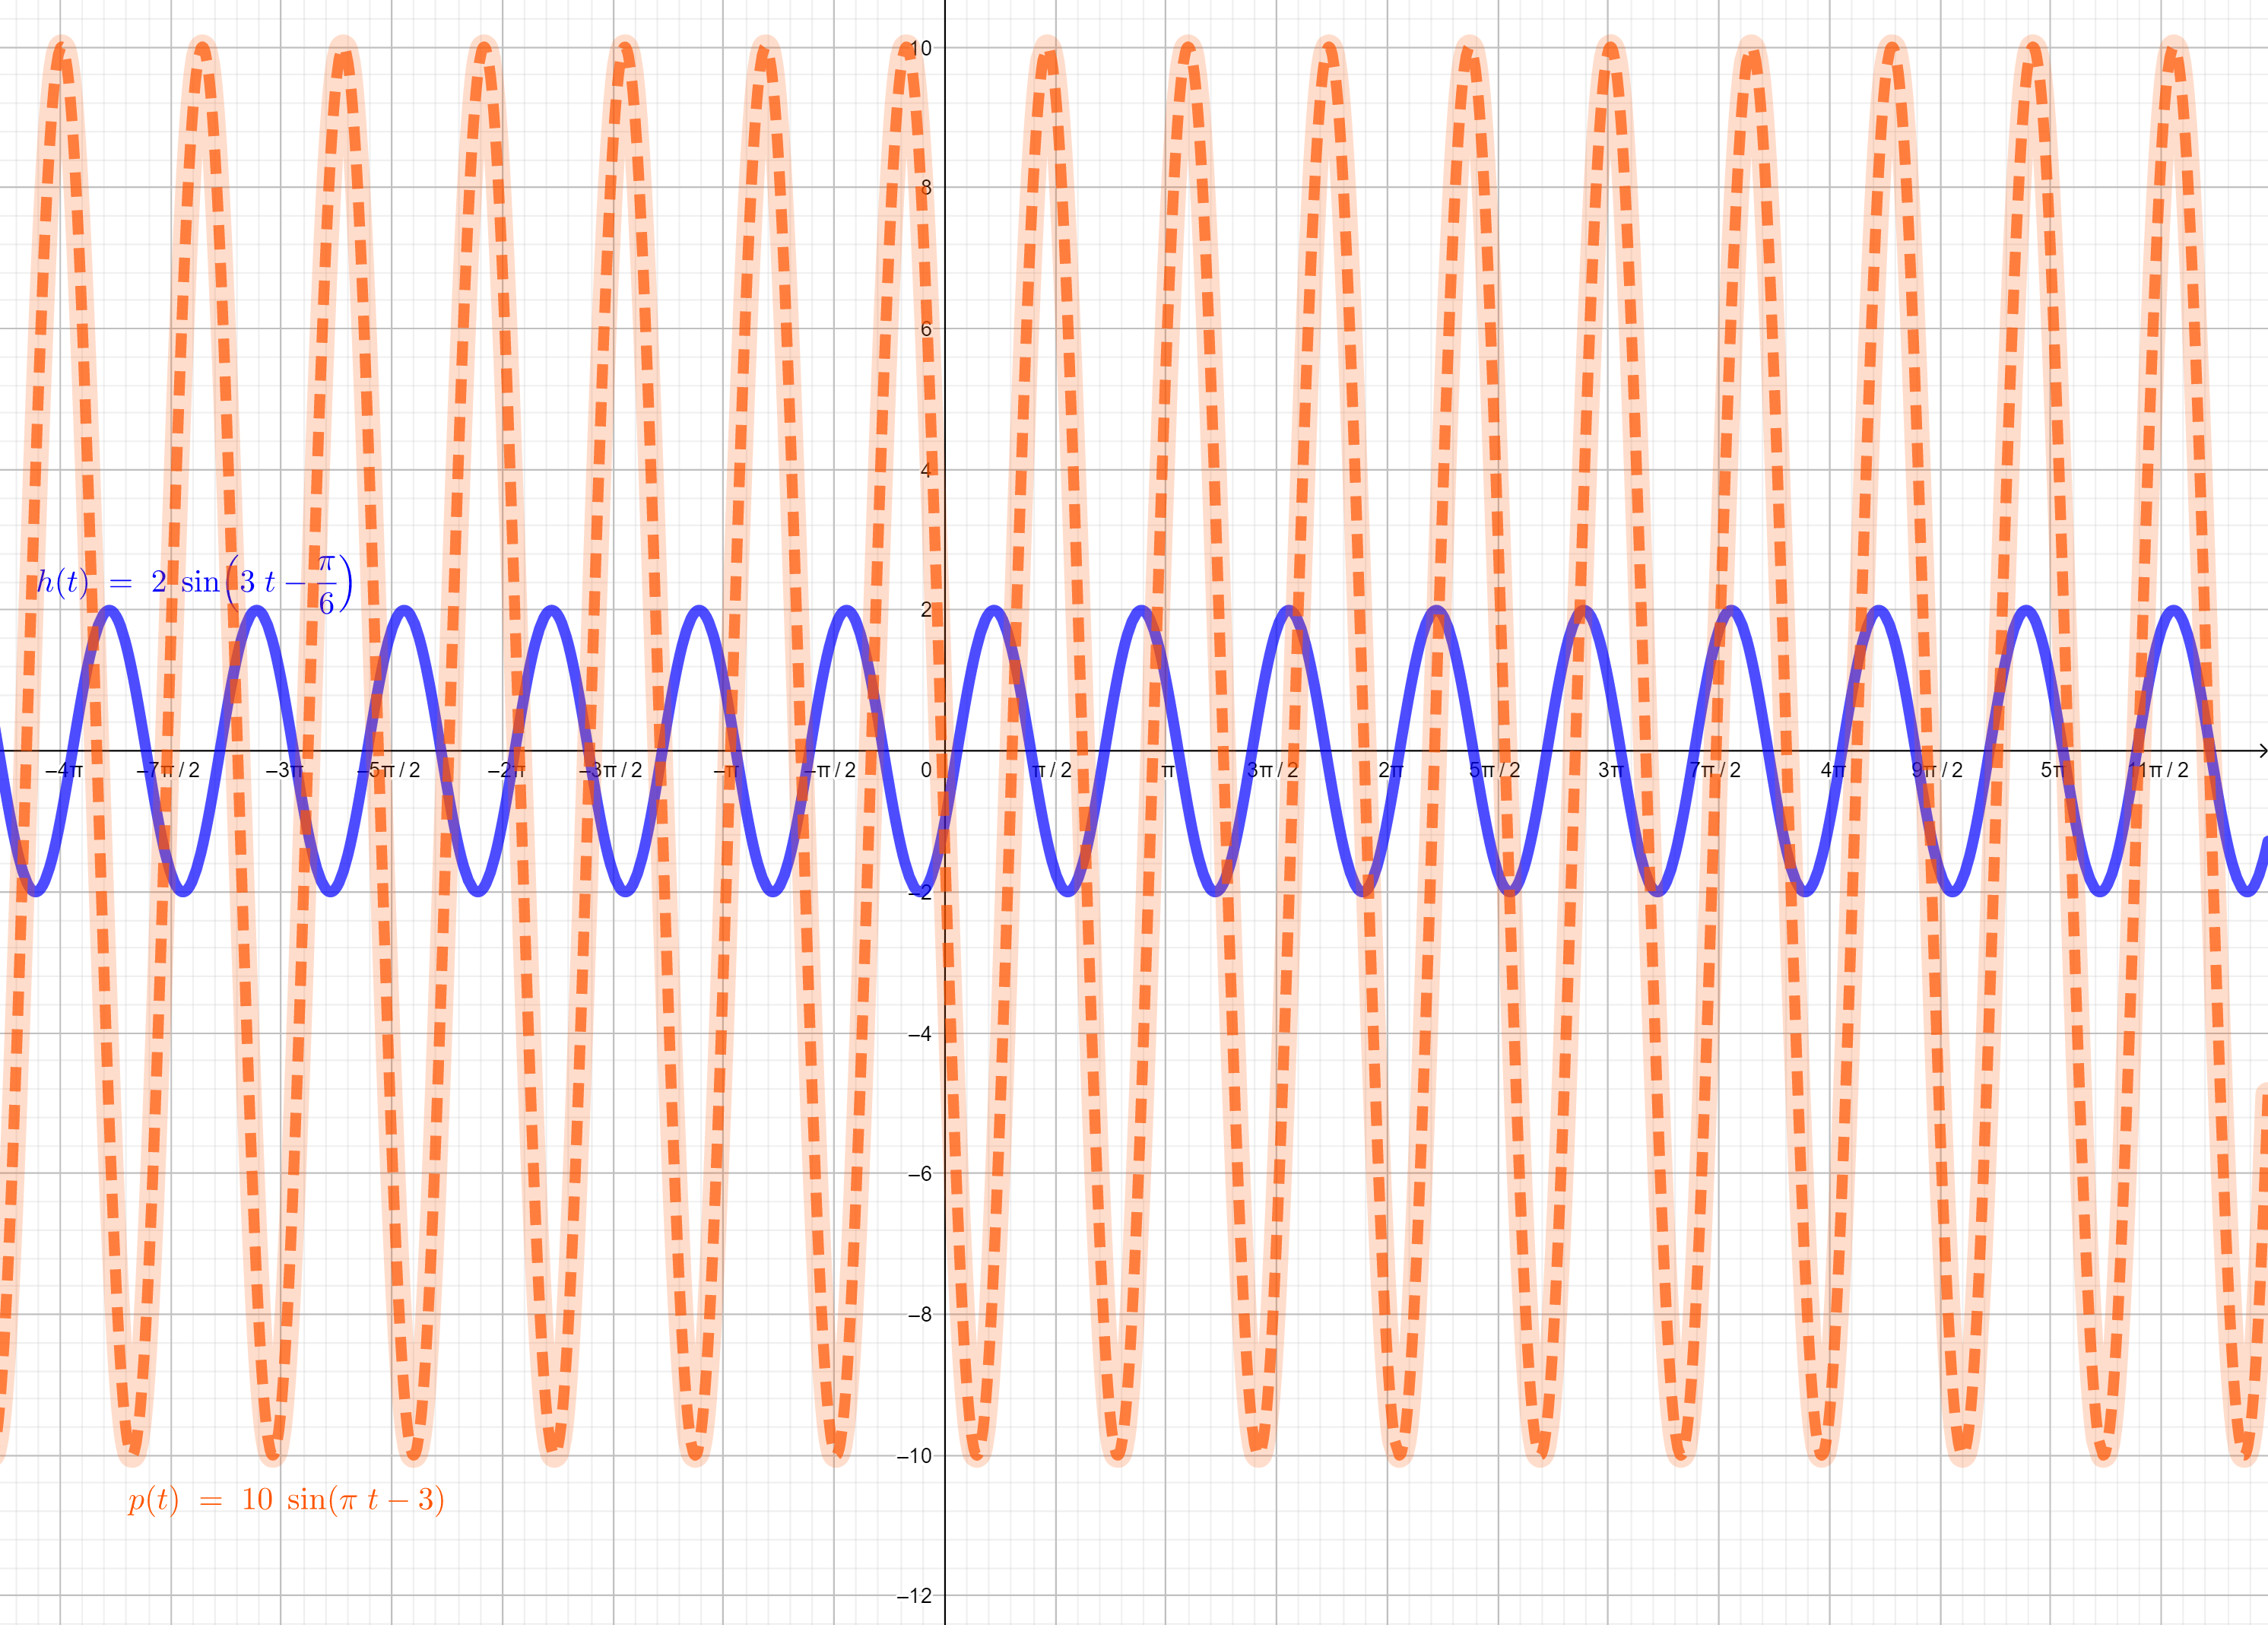
\includegraphics[width=0.8\textwidth]{../Mathematik_1/Bilder/schwingungen_amplitude_periode_phase_loesung.png}
  \end{center}  
  \begin{itemize}
	  \item[(a)] Die Amplitude $A$, die Periode $T$ und die Nullphase $\phi$ sind \[ A=2, \quad T=\frac{2\pi}{3}, \quad \phi=-\frac{\pi}{6} \]
	  \item[(b)]  Die Amplitude $A$, die Periode $T$ und die Nullphase $\phi$ sind \[ A=10, \quad T=\frac{2\pi}{\pi}=2, \quad \phi=-3 \]
  \end{itemize}
\end{exercisebox}

\begin{exercisebox}[Interpolation] %Andreas
	Eine Funktion der Form \[ f: x\mapsto \frac{a_0}{2} + a_1 \cos(x) + b_1\sin(x)\] soll durch die Punkte $(x_i, y_i),\, i=1,2,3$ mit \[ (0|1), (\pi/6|-1), (\pi/2|-3)\]
	gelegt werden. Bestimmen Sie ein Gleichungssystem f�r die Koeffizienten $a_0, a_1, b_1$ und l�sen Sie es.

  \hspace{0.3cm}
  \newline
  \textbf{L�sung:}
  Allgemein muss gelten 
  \begin{eqnarray*}
	  \left( \begin{array}{ccc} 1/2 & \cos x_1 & \sin x_1 \\ 1/2 & \cos x_2 & \sin x_2 \\ 1/2 & \cos x_3 & \sin x_3 \end{array}\right) \cdot  \left( \begin{array}{c} a_0 \\ a_1 \\ a_2 \end{array}\right) =  \left( \begin{array}{c} y_1 \\ y_2 \\ y_3 \end{array}\right)  
  \end{eqnarray*}
  Im speziellen Fall ergibt sich 
  \begin{eqnarray*}
	  \left( \begin{array}{ccc} 1/2 & 1 & 0 \\ 1/2 & \sqrt{3}/2 & 1/2 \\ 1/2 & 0 & 1 \end{array}\right) \cdot  \left( \begin{array}{c} a_0 \\ a_1 \\ a_2 \end{array}\right) =  \left( \begin{array}{c} 1 \\ -1 \\ -3 \end{array}\right)  
  \end{eqnarray*}
  Die L�sung lautet $ a_0=2, \; a_1=0, \; a_2=-4 $ und f�r die Funktion $f(x) = 1-4\sin(x)\,.$
\end{exercisebox}

\begin{exercisebox}[Gleichungen] %Andreas
	Bestimmen Sie alle L�sungen der folgenden Gleichungen:
	\begin{eqnarray*}
		\begin{array}{ll}
			(a) \; \sin(2x+5) = 0,4 \quad \quad \quad & (b) \;\tan\left( 2(x+1)\right) = 1 \\[1ex] (c)\; \sqrt{\cos(x-1)} = 2^{-1/4} \quad \quad \quad & (d) \; \sin(x) = \sqrt{1-\sin^2(x)} 
		\end{array}
	\end{eqnarray*}

  \hspace{0.3cm}
  \newline
  \textbf{L�sung:}
  \begin{itemize}
	  \item[(a)] Substituiere $u=2x+5$. Dann gilt $\sin(u)=0,4$ falls 
	  \[ u=\arcsin(0,4) + 2k\pi \;\textnormal{oder}\; u=\pi-\arcsin(0,4)+2k\pi, \]
		  $k\in \mathbb Z$. Wegen $x=(u-5)/2$ l�sen 
		  \[ x=\left( \arcsin(0,4) +2k\pi -5\right)/2 \;\textnormal{oder}\; x=\left(\pi -  \arcsin(0,4) +2k\pi -5\right)/2 \] die Gleichung.
	  \item[(b)] $u=2(x+1)$. Dann gilt $\tan(u) =1$ falls 
		  \[ u=\pi/4 + k\pi, \quad k\in \mathbb Z\,. \] 
		  Wegen $x=u/2-1$ folgt \[ x=\pi/8 + k\pi/2-1, \quad k\in \mathbb Z\,.\]
	  \item[(c)] Es gilt \begin{eqnarray*} \sqrt{\cos(x-1)} &=& 2^{-1/4} \quad |\cdot^2 \\ \Rightarrow \quad \cos(x-1) &=& 1/\sqrt{2} \end{eqnarray*} 
		  Setze $u=x-1$. Dann gilt $\cos(u) = 1/\sqrt{2}$ falls \[ u=\pi/4+2k\pi\quad \textnormal{oder}\quad u=-\pi/4 + 2k\pi, \quad k\in \mathbb Z\,.\] 
		  Mit $x=u+1$ folgt \[ x= \pi/4+1+2k\pi \quad \textnormal{oder}\quad x=1-\pi/4+2k\pi,\quad k\in \mathbb Z\,.\]
	  \item[(d)] Es gilt \begin{eqnarray*} \begin{array}{l rcl l} & \sin(x)&=& \sqrt{1-(\sin(x))^2} \quad &|\cdot^2 \\ \Rightarrow & (\sin(x))^2 &=& 1-(\sin(x))^2 &\\ \Leftrightarrow & (\sin(x))^2 &=& 1/2 & |\sqrt{\cdot} \\ \Leftrightarrow & \sin(x) &=& \pm 1/\sqrt{2} \end{array}\end{eqnarray*}
		  Wegen der ersten Gleichung muss $\sin(x)$ nichtnegativ sein, da die Wurzel auf der rechen Seite immer nichtnegativ ist. Daher muss $\sin(x)=1/\sqrt{2}$ gelten. Die L�sungen sind 
		  \[ x=\pi/4+2k\pi \quad \textnormal{oder}\quad x=3\pi/4+2k\pi,\quad k\in \mathbb Z\,.\] 
		  Die Probe ergibt 
		  \begin{eqnarray*} \sin(\pi/4 +2k\pi) &=& \sin(\pi/4) = 1/\sqrt{2} \\\sqrt{1-(\sin(\pi/4+2k\pi))^2} &=& \sqrt{1-1/2} = 1/\sqrt{2} \end{eqnarray*} 
		  und analog 
		  \begin{eqnarray*} \sin(3\pi/4 +2k\pi) &=& \sin(3\pi/4) = 1/\sqrt{2} \\\sqrt{1-(\sin(3\pi/4+2k\pi))^2} &=& \sqrt{1-1/2} = 1/\sqrt{2} \end{eqnarray*} 
		  Demnach sind alle L�sungen durch  \[ x=\pi/4+2k\pi \quad \textnormal{oder}\quad 3\pi/4 + 2k\pi,\quad k\in \mathbb Z\] gegeben.
  \end{itemize}
\end{exercisebox}

\begin{exercisebox}[Kreisgleichung] %Lucy
	Bestimmen Sie die Schnittpunkte der angegebenen Geraden $g$ mit dem Kreis $k:=\{(x,y):\; x^2+y^2=4\}$:
	\begin{eqnarray*}
		\begin{array}{lll}
		(a)\; g_1: x\mapsto x-2 \quad\quad (b) \; g_2: x\mapsto x-4 \quad\quad (c)\; g_3: x\mapsto 2 \end{array}
	\end{eqnarray*}


  \hspace{0.3cm}
  \newline
  \textbf{L�sung:}
	\begin{itemize}
		\item[(a)] Zu l�sen ist die quadratische Gleichung $x^2-2x=0$. F�r $x_1=0$ erh�lt man den ersten Schnittpunkt $S_1=(0,-2)$ und f�r $x_2=2$ erh�lte man den zweiten Schnittpunkt $S_2=(2|0)$.
		\item[(b)] Zu l�sen ist die quadratische Gleichung $x^2-4x+6=0$. Diese hat keine reellen L�sungen, also schneiden sich Kreis und Gerade nicht.
		\item[(c)] Zu l�sen ist die quadratische Gleichung $x^2 = 0$. Die L�sung $x=0$ f�hrt auf den Schnittpunkt $(0,2)$.
	\end{itemize}
\end{exercisebox}

\begin{exercisebox}[Kreisgleichung] %Lucy
	Welche der Gleichungen beschreiben einen Kreis? Bestimmen Sie gegebenenfalls die Mittelpunkte und die Radien.
			\begin{eqnarray*} 
				\begin{array}{lll} 
					(a) \; (x+2)^2 + y^2 = 64 \quad \quad & (b)\; (x-5)^2 + (y+2)^2 = 0 \quad \quad & (c) \; x^2 + y^2 - 2x + 4y -20 = 0 \\[1ex] (d) \;x^2 + y^2 - 2x + 2y + 14 = 0 \quad \quad & (e) \; x^2 + y^2 +y = 0 &
				\end{array}
			\end{eqnarray*}

  \hspace{0.3cm}
  \newline
  \textbf{L�sung:}
	\begin{itemize}
		\item[(a)] $(x+2)^2 + y^2 = 64 $ Kreis mit Radius $8$ und Mittelpunkt $M(-2|0)$ %b 
		\item[(b)] $(x-5)^2 + (y+2)^2 = 0 $ Diese Gleichung bestimmt einen einzigen Punkt, n�mlich $P(5|-2)$ %c
		\item[(c)] $x^2 + y^2 - 2x + 4y -20 = 0 \Leftrightarrow (x-1)^2+(y+2)^2 = 20$ Kreis mit Radius $\sqrt{20}$ und Mittelpunkt $M(1|-2)$ %e
		\item[(d)] $x^2 + y^2 - 2x + 2y + 14 = 0$ Diese Gleichung bestimmt weder Kurve noch Punkt %f
		\item[(e)] $x^2 + y^2 +y = 0 \Leftrightarrow x^2 + \left( y+\frac12\right)^2 = \frac{1}{4}$ Kreis mit Radius $\frac12$ und Mittelpunkt $M(0|-\frac12)$ %j
	\end{itemize}
\end{exercisebox}

\begin{exercisebox}[Qualitativer Graph] %Lovis
	\begin{itemize}
		\item[(a)] Zeichnen Sie die Funktion $f: x\mapsto 2\cdot \sin(x-\frac{\pi}{2})-2$ auf dem Intervall  $[-\pi,3\pi]$ und lesen Sie aus dem Graphen den Bildbereich, die Nullstellen und die Extremstellen von $f$ ab.
		\item[(b)] Zeichnen Sie die Funktion $f: x\mapsto -\sin(x-\pi)$ auf dem Intervall  $[0,\frac{5\pi}{2}]$ und lesen Sie aus dem Graphen den Bildbereich, die Nullstellen und die Extremstellen von $f$ ab.
	\end{itemize}

  \hspace{0.3cm}
  \newline
  \textbf{L�sung:}
	\begin{itemize}
		\item[(a)] Die Sinuskurve ist entlang der $x$-Achse um $\pi/2$ nach rechts und entlang der $y$-Achse um $2$ nach oben verschoben und hat die Amplitude $2$. Der Wertebereich ist $[-4,0]$, die Nullstellen sind $\{-\pi,\pi,3\pi\}$ und die Extremstellen sind $\{-\pi, 0, \pi, 2\pi, 3\pi\}$.
		\item[(b)] Die Sinuskurve ist entlang der $x$-Achse um $\pi$ nach rechts und an $y$-Achse gespiegelt. Der Wertebereich ist $[-1,1]$, die Nullstellen sind $\{0,\pi,2\pi\}$ und die Extremstellen sind $\{\frac{\pi}{2}, \frac{3\pi}{2}, \frac{5\pi}{2}\}$.
	\end{itemize}
\end{exercisebox}
 \newpage 
\setcounter{exercise}{0}\pagestyle{empty} \section*{Komposition von Funktionen Aufgaben mit L�sungen}\label{MA1-verkettung-von-funktionen-loesungen}

\ifintegriereaufgaben
	Regeln und Beispiele, die zum Verst�ndnis der L�sungswege hilfreich sind, finden Sie im Skript\wennreferenzvorhanden{MA1-verkettung-von-funktionen}{ (Abschnitt \abschnittsverweis{MA1-verkettung-von-funktionen})}.
\else
	Regeln und Beispiele, die zum Verst�ndnis der L�sungswege hilfreich sind, finden Sie im Skript.
\fi 

%\begin{exercisebox}[Verkettung]  %Moodle
%	Wenn $b\circ c$ die Funktion $2\cdot c + b$ ist, welche Funktion muss dann $b$ bezeichnen, damit $b\circ c = c\circ b$ ?
%\end{exercisebox}

\begin{exercisebox}[Verkettungen]
	Bestimmen Sie Funktionen $u_1, u_2$ so, dass $f=u_1\circ v_1 = u_2\circ v_2$ ist:
  \begin{itemize}
    \item[(a)] $f(x) = (2x+6)^3, \quad v_1(x) = 2x+6, \quad v_2(x) = x+3$
    \item[(b)] $f(x) = \frac{3}{(x-1)^2}, \quad v_1(x) = x-1, \quad v_2(x) = (x-1)^2$
  \end{itemize}

  \hspace{0.3cm}
  \newline
  \textbf{L�sung:}
  \begin{itemize}
	  \item[(a)] $u_1(x) = x^3$, $u_2(x) = (2\cdot x)^3$
	  \item[(b)] $u_1(x) = \frac{3}{x^2}$, $u_2(x) =  \frac{3}{x}$
  \end{itemize}
\end{exercisebox}


\begin{exercisebox}[Definitionsbereich]
  Geben Sie den maximalen Definitionsbereich der Funktion $u\circ v$ an
  \begin{itemize}
    \item[(a)] $u(x) = \sqrt{x}, \quad v(x) = 3-x$
    \item[(b)] $u(x) = \frac{1}{x}, \quad v(x) = 4-x^2$
    \item[(c)] $u(x) = \sqrt{1-x}, \quad v(x) = x^2$
  \end{itemize}

  \hspace{0.3cm}
  \newline
  \textbf{L�sung:}
  \begin{itemize}
	  \item[(a)] $ (u\circ v)(x) = \sqrt{3-x} \; \Rightarrow \; D_{u\circ v} = (-\infty,3]$
	  \item[(b)] $ (u\circ v)(x) = \frac{1}{4-x^2} \; \Rightarrow \; D_{u\circ v} = \mathbb R \setminus \{-2, 2\}$
	  \item[(c)] $ (u\circ v)(x) = \sqrt{1-x^2} \; \Rightarrow \; D_{u\circ v} = [-1,1]$
  \end{itemize}
\end{exercisebox}

\begin{exercisebox}[Definitionsbereich]
	Gegeben sind die Funktionen $v: \mathbb R^+ \to \mathbb R,\; x\mapsto \ln(x)$ und $u:[0,2\pi] \to \mathbb [-1,1], \,x\mapsto \sin(x)$. Betrachten Sie die Funktion $f:u \circ v$. Geben Sie den maximalen Definitionsbereich von $f$ an. 
  \hspace{0.3cm}
  \newline
  \textbf{L�sung:}
  Da der Logarithmus nur positive Zahlen verarbeitet, darf der Definitionsbereich der Funktion $f$ keine $x$ enthalten, f�r die der Sinus $\leq 0$ liefert. Es gilt $\sin(x) > 0 \Leftrightarrow x \in (0,\pi)$ und damit  \[ v\circ u: \;  (0,\pi) \to (-\infty, 0], \; x\mapsto \ln\left( \sin(x)\right)\,.\] 
\end{exercisebox}

\begin{exercisebox}[$g:x\mapsto 0,7\cdot (x+2)^{-2} +4$]
	Gegeben sind die Funktionen $f:x\mapsto x^{-2}$ und $g:x\mapsto 0,7\cdot (x+2)^{-2} +4$.
	\begin{itemize}
		\item[(a)] Geben Sie den Definitions- und den Bildbereich der Funktionen $f$ und $g$ an. 
		\item[(b)] Beschreiben Sie, wie die Funktion $g$ aus der Funktion $f$ hervorgeht. 
		\item[(c)] Bestimmen Sie die Asymptoten der Funktionen $f$ und $g$.
	\end{itemize}

  \hspace{0.3cm}
  \newline
  \textbf{L�sung:}
  \begin{center}
	  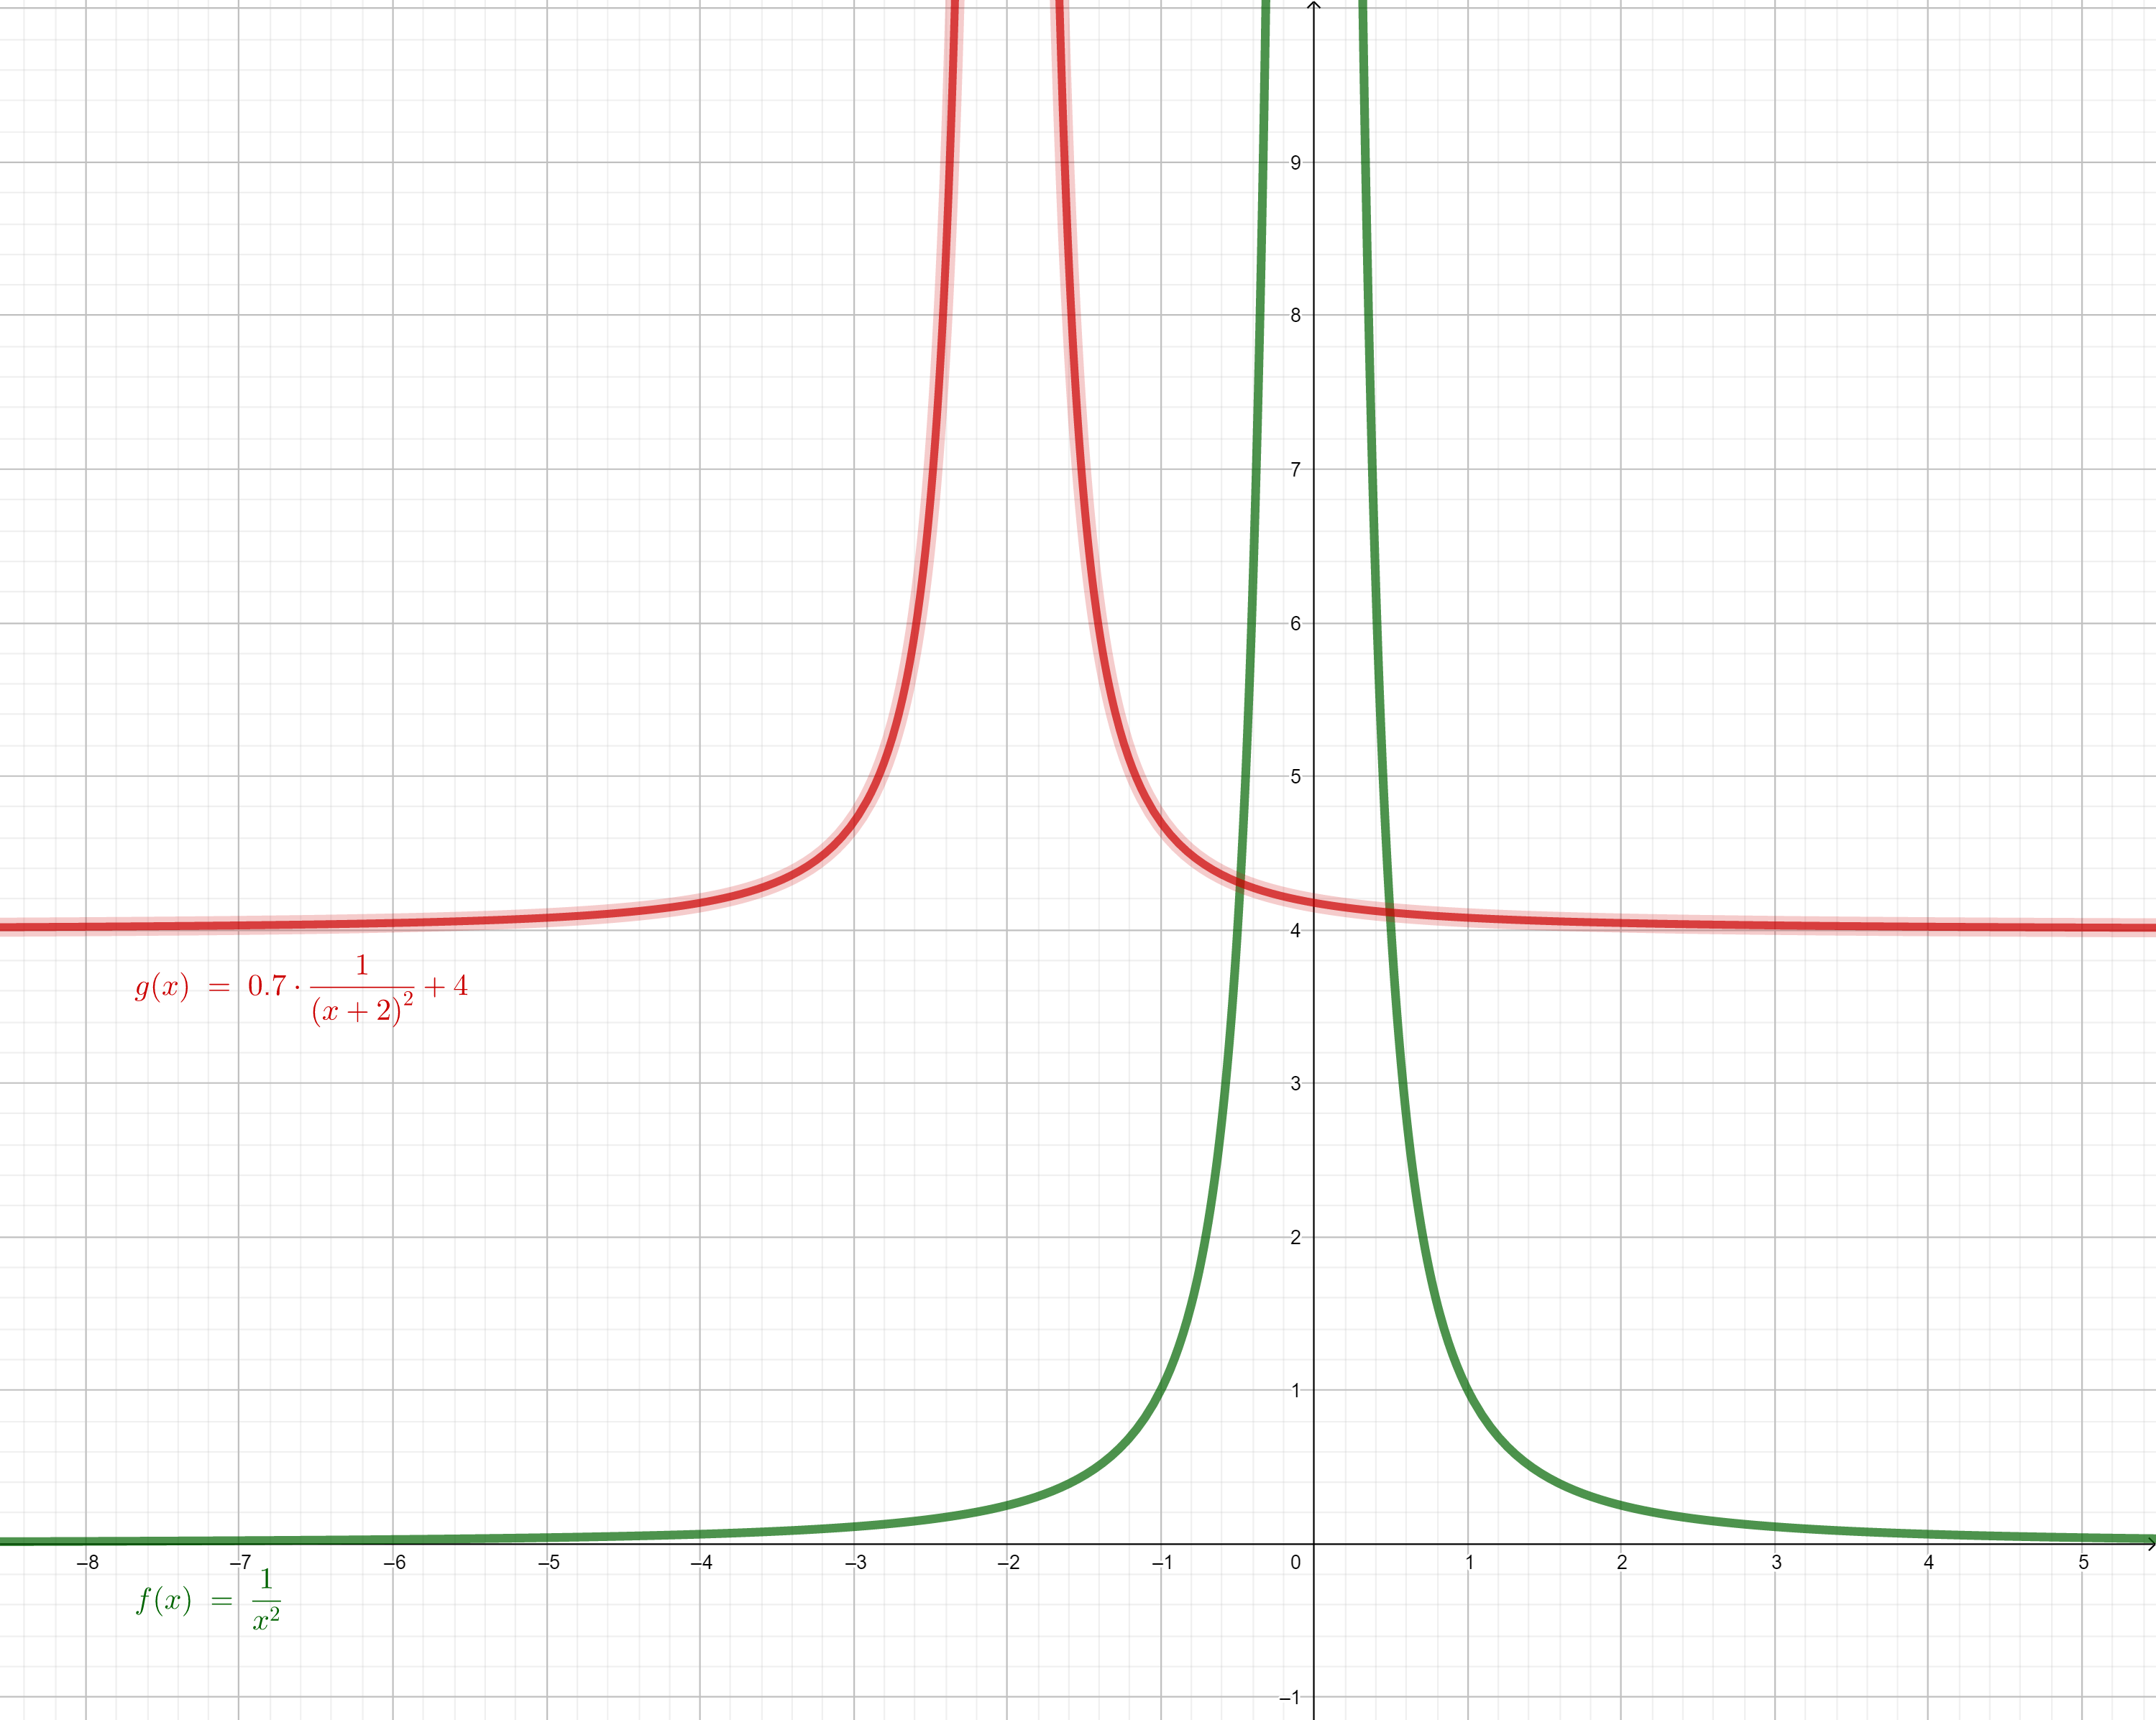
\includegraphics[width=0.6\textwidth]{../Mathematik_1/Bilder/rationale_funktionen_transformation_inverse_quadratfunktion_loesung.png}
  \end{center}
	\begin{itemize}
		\item[(a)] $f: \mathbb R\setminus\{0\} \to (0,\infty)$, $g: \mathbb R\setminus\{-2\} \to (4,\infty)$, 
		\item[(b)] Der Funktionsgraph von $f$ wird entlang der $x$-Achse um zwei Einheiten nach links verschoben und um den Faktor $0,7$ vertikal gestaucht und schlie�lich entlang der $y$-Achse um vier Einheiten nach oben verschoben. 
		\item[(c)] Horizontale Asymptoten: $w_f:x\mapsto 0, \; w_g:x\mapsto 4$; $f$ hat eine vertikale Asymptote an der Stelle $x^*=0$ und $g$ entsprechend an der Stelle $x^*=-2$.
	\end{itemize}
\end{exercisebox}

\begin{exercisebox}[Manipulationen eines Graphen]
	Gegeben sei eine Funktion $f:\mathbb R \to \mathbb R, x\mapsto f(x)$. Geben Sie die Abbildungsvorschrift an, die man auswerten muss, um den Graphen von $f$ \dots
	\begin{itemize}
		\item[(a)] um den Faktor $5$ horizontal zu stauchen: $x\mapsto f\left(5\cdot x\right)$,
		\item[(b)] um den Faktor $\pi$ vertikal zu strecken: $x\mapsto \pi\cdot f\left(x\right)$,
		\item[(c)] um $2$ L�ngeneinheiten horizontal nach links zu verschieben: $x\mapsto f(x+2)$,
		\item[(d)] um $3\sqrt{7}$ L�ngeneinheiten vertikal nach oben zu verschieben: $x\mapsto f(x)+3\sqrt{7}$
		\item[(e)] um den Graphen an der $x$-Achse zu spiegeln:  $x\mapsto -f(x)$.
	\end{itemize}
\end{exercisebox}

\begin{exercisebox}[Anwendung: Temperaturskalen]
  Temperaturangaben der Kelvin Skala rechnet man in solche der Celsius Skala um nach der Vorschrift $x\mapsto x- 273$, solche der Celsius Skala in die Fahrenheit Skala durch $x\mapsto 1,8x+32$. Wie lautet die Vorschrift, um von der Kelvin Skala direkt in die Fahrenheit Skala umzurechnen?

  \hspace{0.3cm}
  \newline
  \textbf{L�sung:}
  Es ist $T_{\mathrm K\to \mathrm C}: x\mapsto x- 273$ und  $T_{\mathrm C\to \mathrm F}: x\mapsto 1,8\cdot x- 32$. Also $T_{\mathrm K\to \mathrm F} =  T_{\mathrm C\to \mathrm F} \circ T_{\mathrm K\to \mathrm C}: x\mapsto  1,8\cdot ( x-273) - 32 = 1,8 \cdot x - 523,4$.
\end{exercisebox}

 \newpage 
\setcounter{exercise}{0}\pagestyle{empty} \section*{Komplexe Zahlen I}\label{MA1-komplexe-zahlen-grundlagen-loesungen}

\ifintegriereaufgaben
	Regeln und Beispiele, die zum Verst�ndnis der L�sungswege hilfreich sind, finden Sie im Skript\wennreferenzvorhanden{MA1-komplexe-zahlen-grundlagen}{ (Abschnitt \abschnittsverweis{MA1-komplexe-zahlen-grundlagen})}.
\else
	Regeln und Beispiele, die zum Verst�ndnis der L�sungswege hilfreich sind, finden Sie im Skript.
\fi 

\begin{exercisebox}[Rechenregeln] %Andreas
	Gegeben sinde die komplexen Zahlen $z_1: = -2 + 4i$ und $z_2:= 1-3i$.
	\begin{itemize}
		\item[(a)] Berechnen Sie $\quad i\cdot z_1 - 2 \cdot z_2, \quad z_1 \cdot z_2, \quad \displaystyle{\frac{z_1}{z_2}}, \quad \displaystyle{\frac{2z_1 z_2}{z_1^2+z_2^2}}$.
		\item[(b)] Bestimmen Sie $\quad |z_1|,\quad |z_2|,\quad |z_1\cdot z_2|$.
		\item[(c)] Bestimmen Sie $\quad \overline{z_1},\quad \overline{z_2},\quad \overline{z_1}\cdot \overline{z_2}$.
		\item[(d)] Stellen Sie die folgenden Zahlen in der kartesischen Form dar ($a,b\in\mathbb R$):
			\[ \frac{3-21i}{4-3i} + 3(i-8), \quad (2-4i)^2+\frac{|1-\sqrt{3}i|}{i}, \quad \left| \frac{a+bi}{a-bi} + \frac{a-bi}{a+bi}\right| \]
	\end{itemize}
  \textbf{L�sung:}
  \begin{itemize}
	  \item[(a)] $-6+4i, \quad  10+2i, \quad -\dfrac{7}{5} - \dfrac{1}{5}i, \quad \dfrac{2z_1 z_2}{z_1^2+z_2^2} = \dfrac{-132+90i}{221}$
	  \item[(b)] $\sqrt{20}, \quad \sqrt{10}, \quad \sqrt{200}$
	  \item[(c)] $\overline{z_1}=-2-4i, \quad \overline{z_2}= 1+3i, \quad  \overline{z_1}\cdot \overline{z_2} =10-10i$
	  \item[(d)] $-21, \quad -12 + 18i, \quad 2\Big|\displaystyle{\frac{a^2-b^2}{a^2+b^2}}\Big|$
  \end{itemize}
\end{exercisebox}

\begin{exercisebox}[Ungleichungen] %Lucy
Bestimmen Sie die Punkte $z\in\mathbb C$, die folgende Eigenschaften besitzen:
\begin{itemize}
	\item[(a)] $0<|z+i|<2$ 
	\item[(b)] $|z-z_1| = |z-z_2|$ 
	%\item $|z|=1$ (Kreislinie)
	%\item $|z|\leq 1$ (Kreisschreibe)
	%\item $|z|> 1$  %($\mathbb R^2 \setminus \{\textnormal{Kreisschreibe}\}$)
	%\item $0<\mathrm{arg}( z) < \pi/4$  %(Ecke, $\sin(\pi/4) = \cos(\pi/4)$)
% 	\item $\mathrm{Re}\frac{1}{z} = \frac{1}{2a}, \quad a>0, a\in \mathbb R$ (verschobene Kreislinie)\par
%
%			Beachte:
%			\begin{eqnarray*}
%				\frac{1}{x+iy} = \frac{x+iy}{x^2 - y^2} = \frac{x}{x^2 + y^2} -i \frac{y}{x^2 + y^2} = \frac{x}{x^2 + y^2}  
%			\end{eqnarray*} 
%			Also:
%               \begin{eqnarray*}
%	            \mathrm{Re}\left( \frac{1}{x+iy}\right) = \frac{x}{x^2-y^2} &=& \frac{1}{2a} \\
%	            \Leftrightarrow 2ax &=& x^2 + y^2 \Leftrightarrow  x^2 - 2ax + a^2 - a^2 + y^2 = 0 \\
%	            \Leftrightarrow (x-a)^2 + y^2 &=& a^2
%                \end{eqnarray*}
	\item[(c)] $ |z^2-\overline z^2| \geq 4 $
	%\item[(d)] $ |z^2+\overline z^2| \geq 4 $
	%\item[(e)] Welche Punktmenge der Gau�'schen Zahlenebene erf�llen (c) und (d)?
	\end{itemize}
  \textbf{L�sung:}
  \begin{itemize}
	  \item[(a)] Die Menge aller $z\in\mathbb C$ mit $0<|z+i|<2$ entspricht einer Kreisscheibe mit Radius $2$, deren Mittelpunkt  $M(0|-i)$ ist. Der Mittelpunkt selbst ist in der Menge nicht enthalten.
			\begin{eqnarray*}
				0^2 = 0 <  (z+i)\overline{(z+i)}  = (x+i (y+1))\cdot(x-i(y+1)) = x^2+(y+1)^2 < 2^2=4  
			\end{eqnarray*}
	\item[(b)] Die Menge aller Punkte $z\in\mathbb C$ mit $|z-z_1| = |z-z_2|$ sind die Punkte, deren Abstand zu dem gegebenen Punkt $z_1$ gleich gro� ist wie zu dem gegebenen Punkt $z_2$. Also die Mittelsenkrechte zwischen den gegebenen Punkten $z_1$ und $z_2$.
	\item[(c)]  $ \{ z = x+iy \in \mathbb C:   |z^2-\overline z^2| \geq 4 \} $ 
	\begin{eqnarray*}
		 |z^2-\overline z^2|\geq 4 \Leftrightarrow | \underbrace{( z-\overline z)}_{\displaystyle{2\cdot y }} \cdot \underbrace{(z+\overline z)}_{\displaystyle{2\cdot x}}| \geq 4  \Leftrightarrow |4 \cdot x\cdot y |\geq 4 \Leftrightarrow |x\cdot y |\geq 1 
	\end{eqnarray*}
	\begin{minipage}{0.3\textwidth }
	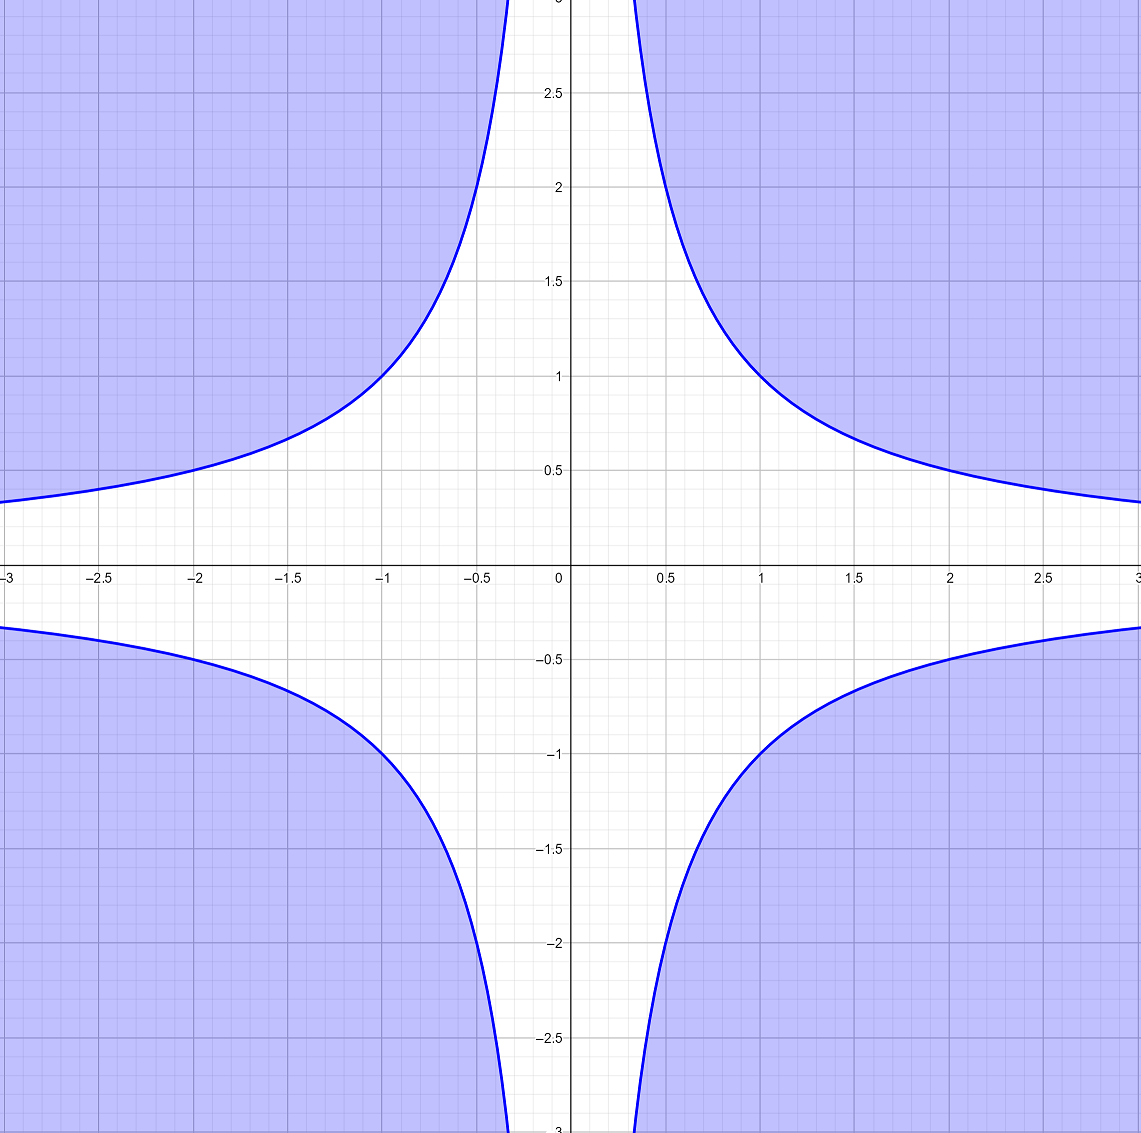
\includegraphics[width=\textwidth]{../Mathematik_1/Bilder/komplexe_zahlen_menge_betrag_xy_loesung.png} \hspace{0.5cm}
\end{minipage}
\begin{minipage}{0.7\textwidth }
	Fallunterscheidung: 
	\begin{eqnarray*}
		\begin{cases} x>0, y>0:\quad |x\cdot y | = x\cdot y {\geq} 1  & \Leftrightarrow y \geq \displaystyle{\frac1x} \\[1ex]
			x>0, y<0:\quad |x\cdot y | = -x\cdot y {\geq} 1 & \Leftrightarrow y \leq -\displaystyle{\frac1x} \\[1ex] 
			x<0, y>0:\quad |x\cdot y | = -x\cdot y {\geq} 1 & \Leftrightarrow y \geq -\displaystyle{\frac1x} \\[1ex]
		x<0, y<0:\quad |x\cdot y | = x\cdot y {\geq} 1  & \Leftrightarrow y \leq \displaystyle{\frac1x}  
	\end{cases}
	\end{eqnarray*}
\end{minipage}
  \end{itemize}
\end{exercisebox}
%\item[(d)]  $ \{ z = x+iy \in \mathbb C:   |z^2+\overline z^2| \leq 4 \} $ 
%	\begin{eqnarray*}
%		 |z^2+\overline z^2|\geq 4 \Leftrightarrow | ( x+iy)^2 + (x-iy)^2| \leq 4  \Leftrightarrow | 2\cdot x^2 - 2 \cdot y^2 |\leq 4 \Leftrightarrow |x^2 -  y^2 |\leq 2 
%	\end{eqnarray*}
%	Fallunterscheidung: 
%	\begin{eqnarray*}
%		\begin{cases} 
%			x^2-y^2 < 0 \Leftrightarrow x^2<y^2 \Leftrightarrow |x| < |y|: &\quad |x^2-y^2 | = -x^2+y^2 = {\leq} 2  \\[1ex] & \Leftrightarrow |y|  \leq \sqrt{x^2+2} \Rightarrow \begin{cases} y \leq \sqrt{x^2+2},\; y \geq 0 \\[1ex] y \geq  -\sqrt{x^2+2}, \; y\leq 0 \end{cases} \\[1ex]
%			x^2-y^2 > 0 \Leftrightarrow x^2>y^2 \Leftrightarrow |x| > |y|: &\quad |x^2-y^2 | = x^2-y^2 = {\leq} 2 \\[1ex] & \Leftrightarrow |y|  \geq \sqrt{x^2-2} \Rightarrow \begin{cases} y \geq \sqrt{x^2-2} \land |x|>\sqrt{2},\; y \geq 0 \\[1ex] y \leq  -\sqrt{x^2-2} \land |x|>\sqrt{2} \; y\leq 0 \end{cases} \\[1ex]
%	\end{cases}
%	\end{eqnarray*}
%	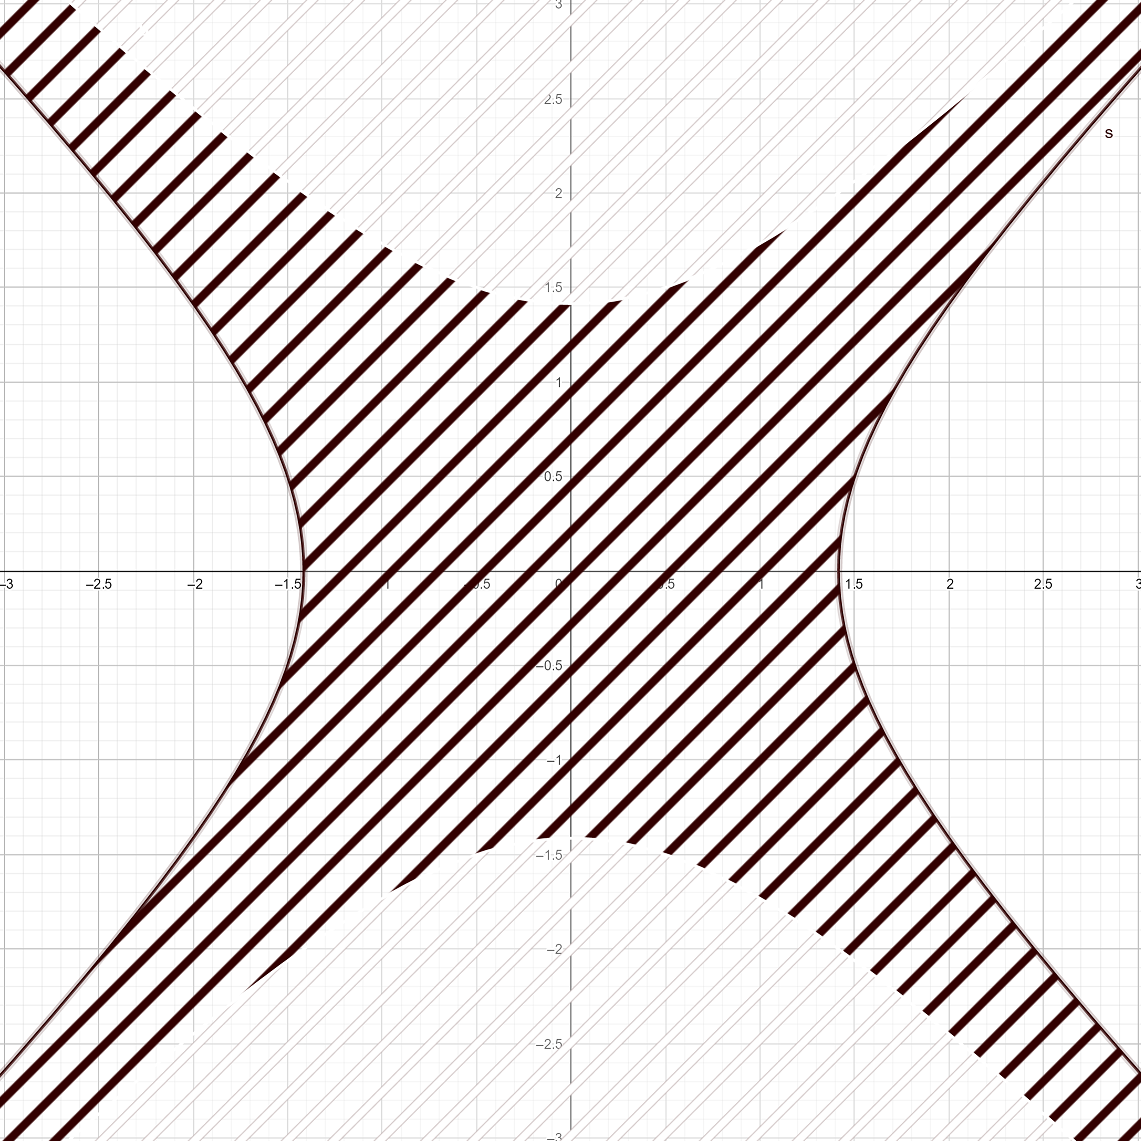
\includegraphics[width=0.3\textwidth]{../Mathematik_1/Bilder/komplexe_zahlen_hyperbelgebiet_schraffur.png} \hspace{0.5cm}
%	\includegraphics[width=0.3\textwidth]{../Mathematik_1/Bilder/komplexe_zahlen_hyperbelgebiet_ueberlagerung.png}

\begin{exercisebox}[Die imagin�re Einheit] %Lucy
	Berechnen Sie $i^{172}$ und $i^{175}$.

  \vspace{0.3cm}
  \textbf{L�sung:}
	\begin{eqnarray*} 
		i^{4m} &=& 1, \; m\in \mathbb N_0 \\
		i^{4m+1} &=& i,  \; m\in \mathbb N_0 \\
		i^{4m+2} &=& -1,  \; m\in \mathbb N_0 \\
		i^{4m+3} &=& -i,  \; m\in \mathbb N_0 \\
		&&\\
		\Rightarrow && i^{172} = \left(i^4\right)^{43} = 1 \\
		\Rightarrow && i^{175} = \left(i^4\right)^{43}\cdot i^3 = -i
	\end{eqnarray*}
\end{exercisebox}

\begin{exercisebox}[Kartesische und Polarkoordinaten] %Andreas
	\begin{itemize}
		\item[(a)] Bestimmen Sie von folgenden komplexen Zahlen die Polarkoordinaten:
			\[ z_1=i,\quad z_2=\sqrt{3}-i, \quad z_3=-1-i, \quad z_4=x-\sqrt{3}x\,i\; (x>0) \]
		\item[(b)] Bestimmen Sie von folgenden komplexen Zahlen die kartesische Form:
			%\[ z_1= 1\cdot e^{-i4\pi/3},\quad z_2=\sqrt{2}a \cdot e^{-i\pi/4} \]
			\[ z_1 \; \widehat =\; \left( 1, -4\pi/3\right) ,\quad z_2 \; \widehat =\; \left( \sqrt{2}a,  -\pi/4\right) \]
	  \end{itemize}

\noindent\textbf{L�sung:}
\begin{itemize}
	\item[(a)] 
\begin{eqnarray*}
	z_1 &\widehat =& \left( 1, \pi/2 \right)\\[1ex]
	z_2 &\widehat =& \left( 2,  \mathrm{atan2}(-1, \sqrt{3})= -\frac{\pi}{6}\right)\\[1ex]
	z_3 &\widehat =& \left(\sqrt{2}, \mathrm{atan2}(-1,-1)=-\frac34\pi \right)\\[1ex]
	z_4 &\widehat =& \left( 2x, \mathrm{atan2}(-\sqrt{3}x,x)=-\frac{\pi}{3} \right)\\[1ex]
\end{eqnarray*}
	\item[(b)] Nach Pythagoras gilt \(a = |z|\cos(\varphi)\) und \(b=|z|\sin(\varphi)\)
%\begin{eqnarray*}
%	z_1 &\widehat =& e^1 \cdot ( \cos(-4\pi/3) + i \sin(-4\pi/3)= -\frac{e}{2} + i \frac{\sqrt{3}e}{2}\\[1ex]
%		z_2 &\widehat =& \sqrt{2}a \cdot ( \cos(-\pi/4) + i \sin(-\pi/4)) = 2a-2ai\,.
%	\end{eqnarray*}
\begin{eqnarray*}
	z_1  &=&  \cos(-4\pi/3) + i \sin(-4\pi/3)= -\frac{e}{2} + i \frac{\sqrt{3}e}{2}\\[1ex]
		z_2 &=& \sqrt{2}a \cdot ( \cos(-\pi/4) + i \sin(-\pi/4)) = 2a-2ai\,.
	\end{eqnarray*}
\end{itemize}
\end{exercisebox}

\begin{exercisebox}[Kartesische und Polarkoordinaten] %Lucy
	Bestimmen Sie mit Hilfe der Polarkoordinaten die kartesische Form der folgenden komplexen Zahl: \[z= \left( \frac12 + \frac{\sqrt{3}}{2}i\right)^{60}\,.\]
\noindent\textbf{L�sung:}
\[ \tilde z = \frac{1}{2} + \frac{\sqrt{3}}{2} i \Rightarrow \; \tilde z \;  \widehat{=} \; \left( 1, \pi/3 \right) \; \Rightarrow z = \tilde z^{60} \; \widehat = \;\left( 1^{60},  60\cdot \pi/4\right) = \left( 1^{60},  20\cdot \pi\right) \Rightarrow \, z = 1\,.\]
\end{exercisebox}

\begin{exercisebox}[Gleichungssystem] %Andreas
	L�sen Sie das folgende lineare Gleichungssystem
	\begin{eqnarray*}
		\begin{array}{r c r c l} 
			(3-4i)\cdot z_1 &+& (2-i)\cdot z_2 &=& 4-7i \\[1ex]
	(1-2i)\cdot z_1 &+& 4i\cdot z_2 &=& -11-15i 
\end{array}
\end{eqnarray*}
  \textbf{L�sung:}
  Die erweiterte Koeffizientenmatrix lautet 
  \begin{eqnarray*}
	  &\left( \begin{array}{cccc} 3-4i & 2-i &|& 4-7i \\ 1-2i & 4i & | & -11-15i \end{array}\right) \\
	  \stackrel{(*)}{ \Leftrightarrow} \;& \left( \begin{array}{cccc} 3-4i & 2-i &|& 4-7i \\ 0 & -0.8 + 4.6i & | & 12.2-11.6i \end{array}\right) 
  \end{eqnarray*}
  wobei $(*)$ die folgende �quivalenzumformung meint: Addiere das $-(1-2i)/(3-4i)$-fache der ersten Zeile zur zweiten Zeile.
  Die zweite Zeile liefert eine lineare Gleichung f�r $z_2$: 
  \begin{eqnarray*} \begin{array}{clcr r}
	  & (-0.8+4.6i) z_2 &=& 12.2-11.6i\; & |:(-0.8+4.6i) \\
	  \Leftrightarrow & z_2 &=& -2+3i 
  \end{array}\end{eqnarray*}
  Setzt man $z_2$ in die erste Zeile ein, so erh�lt man eine lineare Gleichung f�r $z_1$:
  \begin{eqnarray*} \begin{array}{clcr r}
		  & (3-4i)z_1 + (-1+8i) &=& 4-7i\; & |-(-1+8i) \\
		  \Leftrightarrow & (3-4i)z_1 &=& 5-15i \; & |:(3-4i) \\
	  \Leftrightarrow & z_1 &=& 3-i 
  \end{array}\end{eqnarray*}
  Die L�sung lautet $z-1=3-i, \; z_2=-2+3j\,.$
\end{exercisebox}

 \newpage 
\setcounter{exercise}{0}\pagestyle{empty} \section*{Komplexe Zahlen II L�sungen}\label{MA1-komplexe-zahlen-polarform-und-euler-loesungen}

\ifintegriereaufgaben
	Regeln und Beispiele, die zum Verst�ndnis der L�sungswege hilfreich sind, finden Sie im Skript\wennreferenzvorhanden{MA1-komplexe-zahlen-polarform-und-euler}{ (Abschnitt \abschnittsverweis{MA1-komplexe-zahlen-polarform-und-euler})}.
\else
	Regeln und Beispiele, die zum Verst�ndnis der L�sungswege hilfreich sind, finden Sie im Skript.
\fi 

\begin{exercisebox}[Radizieren]
	Bestimmen Sie alle L�sungen der folgenden Gleichungen
	\begin{eqnarray*}
		(a)\; z^3 = -8 \quad \quad \quad 
		(b)\; z^2 = i \quad \quad \quad  
		(c)\; z^4 = -16 
  \end{eqnarray*}

\vspace{0.3cm}
\noindent\textbf{L�sung:}\newline
\begin{itemize}
	\item[(a)] 
		\begin{eqnarray*} 
			-8 = 8 \cdot e^{i\pi}\; \Rightarrow z_k &=& \sqrt[3]{8} \cdot e^{i(\pi+2\pi \,k)/3}, \quad k=0,1,2\\[1ex]
			z_0 &=& 2\cdot e^{i\pi/3} = 1+ \sqrt{3}i\,,\\ 
			z_1 &=& 2\cdot e^{i\pi} = -2\,, \\ 
		z_2 &=& 2\cdot e^{5/3\pi \, i} = 1-\sqrt{3}i\,.
		\end{eqnarray*}
		
	\item[(b)]
  \begin{eqnarray*}
	  i = e^{i\pi/2} \; \Rightarrow z_k &=& e^{i(\pi/2+2\pi \,k)/2}, \quad k=0,1\\[1ex]
    z_0 &=&  e^{i \, \pi/4} = \frac{\sqrt{2}}{2} + i\frac{\sqrt{2}}{2}\,,\\
    z_1 &=&  e^{i \,5 \pi/4} =  -\frac{\sqrt{2}}{2} - i\frac{\sqrt{2}}{2}\,.
  \end{eqnarray*}
	\item[(c)] 
  \begin{eqnarray*}
	  -16 = 16 \cdot e^{i\pi} \; \Rightarrow z_k &=&  \sqrt[4]{16} \,e^{i(\pi+2\pi\,k)/4}, \quad k=0,1,2,3 \\[1ex]
	  z_0 &=&  2 e^{\pi/4 \,i} = 2e^{\pi/4 \,i}=\sqrt{2}+i\sqrt{2}\,,\\
  z_1 &=&  2 e^{3/4\pi \, i}=-\sqrt{2}+i\sqrt{2}\,,\\
  z_2 &=&  2 e^{5/4\pi\,i}=-\sqrt{2}-i\sqrt{2}\,,\\
  z_3 &=&  2 e^{7/4\pi\,i}=\sqrt{2}-i\sqrt{2}
  \end{eqnarray*}
\end{itemize}
\end{exercisebox}

\begin{exercisebox}[Eulersche Identit�t]
Zeigen Sie, dass die folgenden Darstellungen f�r $\sin$ und $\cos$ gelten
			\begin{eqnarray*} 
				(a)\; \sin(\varphi) = \frac{e^{i\varphi} - e^{-i\varphi}}{2i} \quad\quad\quad (b)\;\cos(\varphi) = \frac{e^{i\varphi} + e^{-i\varphi}}{2} 
			\end{eqnarray*}

\vspace{0.3cm}
\noindent\textbf{L�sung:}\newline
\begin{eqnarray*}
	e^{ix} &=& \cos(x) + i \sin(x) \\
	e^{-ix} &=& \cos(-x) + i \sin(-x) = \cos(x) - i \sin(x) \\
	\Rightarrow e^{ix} + e^{-ix} &=& \cos(x) + i \sin(-x) + \cos(x) - i \sin(-x)  = 2 \cos(x) \Rightarrow \frac12  \left( e^{ix} + e^{-ix}  \right) = \cos(x) \\
	\Rightarrow e^{ix} - e^{-ix} &=& \cos(x) + i \sin(-x) - \cos(x) + i \sin(-x)  = 2 i  \sin(x) \Rightarrow \frac{1}{2i}  \left( e^{ix} - e^{-ix}  \right) = \sin(x)
\end{eqnarray*}
\end{exercisebox}

\begin{exercisebox}[Fundamentalsatz]
	Betrachten Sie f�r $n\in \mathbb N$ ein Polynom \[ p:\mathbb C\to \mathbb C, \; z\mapsto p(z)=a_nz^n+a_{n-1}z^{n-1} +\cdots a_1z+a_0\] mit reellen Koeffizenten $a_0, \cdots, a_n\in \mathbb R$ und $a_n\not=0$. 
	\begin{itemize}
		\item[(a)] Zeigen Sie: wenn $z_0 \in \mathbb C$ eine Nullstelle von $p$ ist, dann ist auch $\overline{z_0}$ eine Nullstelle von $p$.
		\item[(b)] Wenden Sie obigen Satz an, um alle Nullstellen des Polynoma \[ p:\mathbb C\to \mathbb C, \; z\mapsto p(z) = z^4-2z^3+2z^2-10z+25 \] zu bestimmen. Zeigen Sie zu erst, dass $z_1= 2+j$ eine Nullstelle ist.
	\end{itemize}

  \hspace{0.3cm}
  \newline
  \textbf{L�sung:}
  \begin{itemize}
	  \item[(a)] Sei $z_0$ eine Nullstelle. Zu zeigen ist $p(z_0)=0 \; \Rightarrow \, p(\overline{z_0}) = 0$:
		  \begin{eqnarray*} p(\overline{z_0}) &=& a_n\left( \overline{z_0}\right)^n +  a_{n-1}\left( \overline{z_0}\right)^{n-1} + \cdots + a_1\overline{z_0} + a_0 \\ 
		                                      &=& a_n\left( \overline{z_0}^n\right) +  a_{n-1}\left( \overline{z_0}^{n-1}\right) + \cdots + a_1\overline{z_0} + a_0 \\ 
						      &=& \overline{\left(a_n z_0^n\right)} +  \overline{\left(a_{n-1} z_0^{n-1}\right)} + \cdots + \overline{a_1z_0} + \overline{a_0} \quad\quad (*)\\
						      &=& \overline{ \underbrace{\left(a_n z_0^n\right) +  \left(a_{n-1} z_0^{n-1}\right) + \cdots + a_1z_0 + a_0}_{\displaystyle{ = p(z_0)=0}}}\\
							      &=& \overline{0} = 0\,.
					      \end{eqnarray*}
					      Die Umformung $(*)$ ist g�ltig, weil alle Koeffizienten reell sind, also $\overline{a_i} = a_i$ f�r alle $i=0,\cdots, n$. 
				      \item[(b)] Wegen Aufgabenteil (a) wissen wir, dass $z_1$ und $z_2=\overline{z_1}$ Nullstellen sind und das gegebene Polynom ohne Rest durch die entsprechenden Linearfaktoren teilbar ist. Man kann nacheinander mit je einem Linearfaktoren dividieren oder gleich das quadratische Polynom betrachten: 
					      \[ (z-z_1) \cdot (z-\overline{z_1}) = (z-(2+i))\cdot (z-(2-i)) = z^2-4z+5\]
					      Die Polynomdivision mit dem quadratische Polynom f�hrt auf 
					      \[ (z^4-2z^3+2z^2-10z+25):(z^2-4z+5) = z^2+2z+5 \]
					      Wir erhalten zwei weitere Nullstellen durch die allgemeine L�sungsformel zu $z_3=-1+2i$ und $z_4=-1-2i$. Die Linearfaktorzerlegung von $p$ lautet \[ p(z) = (z-(2+i))\cdot (z-(2-i)) \cdot (z-(-1+2i))\cdot (z-(-1-2i))\,.\]
  \end{itemize}
\end{exercisebox}

\begin{exercisebox}[Fundamentalsatz]
	\begin{itemize}
		\item[(a)]
	L�sen Sie die Gleichung: $4z^2 + (8+12i)z - 5+11i = 0$.
\item[(b)] Bestimmen Sie alle Nullstellen des komplexen Polynoms $p:z\mapsto z^2+\left(2\sqrt{2}i\right) \cdot z - 2\sqrt{3} i$.
	\end{itemize}

  \hspace{0.3cm}
  \newline
  \textbf{L�sung:}
  \begin{itemize}
	  \item[(a)] Diese Aufgabe l�st man mit Hilfe einer quadratischen Erg�nzung:
	\begin{eqnarray*}
		p(z) &=& \underbrace{4}_{a_2}z^2 + \underbrace{(8+12i)}_{a_1}z \underbrace{- 5+11i}_{a_0} \\
		&=& (2z)^2 + 2\cdot 2z \cdot (2+3i) + (2+3i)^2 -(2+3i)^2-5+11i \\
		&=& (2z+2+3i)^2-i \\
		&&\\
		\Rightarrow && (2z+2 + 3i)^2 = i = e^{i\pi/2} \\
		\Rightarrow && (2z+2+3i)^2 = \begin{cases} e^{i\pi/4} \\ 2z_1+2+3i =  e^{i5/4 \pi} = e^{-i3/4 \pi} \end{cases} \\
		\Rightarrow && z = \begin{cases} \frac12( \frac{1}{\sqrt{2}} - 2 + i(\frac{1}{\sqrt{2}} -3)) \\ 
		                                 \frac12(- \frac{1}{\sqrt{2}} - 2 - i(\frac{1}{\sqrt{2}} +3))  \end{cases}
			\end{eqnarray*}
		\item[(b)] Mit der allgemeinen L�sungsformel erhalten wir 
			\[ 
				z = \dfrac{-2\sqrt{2}i + \omega}{2}\,,
			\]
			wobei \(\omega\) die L�sungen der folgenden Gleichung sind 
			\begin{eqnarray*}
				\omega^2 &=&= (2\sqrt{2}i)^2 - 4\cdot (-2\sqrt{3}i) \\  &=&  -8 + 8\sqrt{3}i = 16\cdot e^{i2/3\pi} \; \widehat = \;  \left( 16, \frac23 \pi\right) \,.
			\end{eqnarray*}
			Die komplexen Wurzeln lauten:
			\[\omega_0 = 8\cdot e^{i\pi/3} = 4+4\sqrt{3}i \quad \lor \quad \omega_1 = 8\cdot e^{i8/3\pi} = 8\cdot e^{-i2/3\pi} = -4-4\sqrt{3}i\] Setzen wir die L�sungen \(\omega_{0,1}\) ein, so erhalten wir  
			
			\[ z_1= \left(-\sqrt{3}-\sqrt{2}\right)i-1 \quad \lor \quad z_2= (\sqrt{3}-\sqrt{2})i+1 \,.\]
  \end{itemize}
\end{exercisebox}


\begin{exercisebox}[Anwendungen: Additionstheoreme]
Zeigen Sie, dass f�r alle $x\in \mathbb R$ gilt
	\begin{eqnarray*}
	(a)\; \sin(x \pm y) = \sin(x)\cdot \cos(y) \pm \cos(x)\cdot\sin(y),\quad \quad (b)\; \cos(3x) = 4 (\cos(x))^3 - 3\cos(x) 
\end{eqnarray*}

\vspace{0.3cm}
\noindent\textbf{L�sung:}\newline
Verwenden wir im Folgenden die Abk�rzungen $c_x:= \cos(x)$ und $s_x:=\sin(x)$. 
\begin{itemize}
	\item[(a)] 
\begin{eqnarray*}
	z:=e^{i(x \pm y)} &=& e^{ix} \cdot e^{\pm iy} = = \left( c_x+is_x\right)\cdot \left(c_y\pm is_y\right) \\ 
	&=& c_xc_y \pm ic_xs_y +is_xc_y \mp s_xs_y = c_xc_y + \mp s_xs_y +i( s_x c_y \pm c_xs_y) \\
	&&\Rightarrow \begin{cases} \cos(x\pm y) = \mathrm{Re}(z) = \cos(x)\cos(y) \mp  \sin(x)\sin(y) \\  \sin(x\pm y) = \mathrm{Im}(z)= \sin(x)\cos(y) \pm \cos(x)\sin(y)   
	\end{cases}
	\end{eqnarray*}
	\item[(b)] 
	\begin{eqnarray*}
		z:= e^{i(3x)} &=& \left( e^{ix} \right)^3= = \left( c_x+is_x\right)^3 \\ 
		&=& c_x^3 + 3i c_x^2 s_x + i^2 3c_x s_x^2 + i^3 s_x^3  \\
		&=& c_x^3 - 3c_x s_x^2 + i( 3 c_x^2 s_x - s_x^3) \\
		&=& c_x^3 - 3c_x (1-c_x^2) + i( 3 (1-s_x^2) s_x - s_x^3) \\
		&&\Rightarrow \begin{cases} \cos(3x) = \mathrm{Re}(z) = 4\cos^3(x) - 3 \cos(x)  \\  \sin(3x) = \mathrm{Im}(z) = 3\sin(x) - 4\sin^3(x)\,.
	\end{cases}
	\end{eqnarray*}
\end{itemize}
\end{exercisebox}

\begin{exercisebox}[Anwendungen: Harmonische Schwingungen]
	Gegeben seien die harmonischen Schwingungen \[ s_1(t) = \sqrt{2} \cdot \sin(10t+\pi/4), \quad s_2(t)=2\cos(10t+\pi/6)\,.\]
	\begin{itemize}
		\item[(a)] Berechnen Sie die �berlagerung von $s_1$ und $s_2$. 
			
			Hinweis: $s_1(t) = \mathrm{Im}\left( \sqrt{2} e^{i\,( 10 t+ \pi/4)}\right), \;s_2(t) = 2\sin(10t + \pi/6+\pi/2) = \mathrm{Im}\left( 2 e^{i\,( 10 t+ 2/3 \pi)}\right)$. 
		\item[(b)] Wie muss eine harmonische Schwingung \[ s_3(t) = A_3\sin(\omega_3 t+ \varphi_3)\] gew�hlt werden, dass die �berlagerung von $s_1$ und $s_3$ eine Amplitude von $1$ und eine Nullphase von $\pi/2$ besitzt?
	\end{itemize}

\vspace{0.3cm}
\noindent\textbf{L�sung (Direkte Anwendung der Formeln m�glich, siehe Unterabschnitt "Harmonische Schwingungen")}

\begin{itemize}
	\item[(a)]
		\begin{eqnarray*}
			s_1(t) + s_2(t) &=& \mathrm{Im}\left( \sqrt{2} e^{i\,( 10 t+ \frac14\pi)} + 2 e^{i\,( 10 t+ \frac23\pi)}\right) \\[1ex]
			&=& \mathrm{Im}\left(\sqrt{2} e^{\frac14 \pi \, i} e^{10 t \, i} + 2 e^{\frac23\pi \, i} e^{10 t \,i} \right) \\[1ex]
				&=& \mathrm{Im}\left(  \left( \sqrt{2} e^{\frac14\pi\,i}  + 2 e^{\frac23\pi\,i} \right)  e^{i\, 10 t} \right) \\[1ex]
				&=& \mathrm{Im}\left(  \left( \sqrt{2} \left((\frac{1}{\sqrt{2}} + i + \frac{1}{\sqrt{2}}\right)  + 2 \left( -\frac12 + \frac{\sqrt{3}}{2} i \right) \right)  e^{i\, 10 t} \right) \\[1ex]
				&=& \mathrm{Im}\left(  \left( 1 + i  -1  \sqrt{3} i \right)  e^{i\, 10 t} \right) \\[1ex]
				&=& \mathrm{Im}\left(  i \left( 1 + \sqrt{3}\right)   e^{i\, 10 t} \right), \quad i=e^{i\pi/2} \\[1ex]
				&=& \mathrm{Im}\left(  \left( 1 + \sqrt{3}\right)  e^{i\,( 10 t + \pi/2 )} \right) \\[1ex]
				&=& \left( 1 + \sqrt{3}\right) \sin( 10 t + \pi/2 )
	\end{eqnarray*}
	\item[(b)] 
		F�r die komplexe Amplitude der �berlagerung gilt \[ A= 1\cdot e^{i\pi/2} = i \]
		Suche $A_3$ so, dass \[ A_1 + A_3 = i \Leftrightarrow A_3 = i + A_1\,.\] Das hei�t \[ A_3 = i-(1+i) = -1 = 1\cdot e^{i\pi}\,. \] Also muss gelten $s_3(t) = \sin(10t+\pi)$.
\end{itemize}
\end{exercisebox}

 \newpage 
\setcounter{exercise}{0}\pagestyle{empty} \section*{Vektoren L�sungen}\label{MA1-vektoren-loesungen}

\ifintegriereaufgaben
	Regeln und Beispiele, die zum Verst�ndnis der L�sungswege hilfreich sind, finden Sie im Skript\wennreferenzvorhanden{MA1-vektoren}{ (Abschnitt \abschnittsverweis{MA1-vektoren})}.
\else
	Regeln und Beispiele, die zum Verst�ndnis der L�sungswege hilfreich sind, finden Sie im Skript.
\fi 

\begin{exercisebox}[Rechenregeln]
	Gegeben seien die Vektoren 
	\[ \boldsymbol a = \left( \begin{array}{c} -4 \\ 3 \end{array}\right)\,, \;  
		\boldsymbol b = \left( \begin{array}{c} 0 \\ -3 \end{array}\right)\,,  \;
	\boldsymbol c = \left( \begin{array}{c} -2 \\ -2 \end{array}\right)\,. \] 
	\begin{itemize}
		\item[(a)] Berechnen Sie folgende Ausdr�cke: 
			\[ -\boldsymbol a + 3\cdot \boldsymbol b, \quad (2\cdot \boldsymbol a - \boldsymbol b) + 3\cdot \boldsymbol c, \quad (3\cdot \boldsymbol c - \boldsymbol b) + 2\cdot \boldsymbol a \]
		\item[(b)] Berechnen Sie die folgenden Betr�ge (L�ngen, Normen): 
			\[ |\boldsymbol a|\,,\quad |\boldsymbol b|\,,\quad |\boldsymbol a+ \boldsymbol b|\,,\quad |-\boldsymbol a+3\cdot \boldsymbol b| \]
		\item[(c)] Bestimmen Sie einen Vektor der L�nge $10$, der in die gleiche Richtung wie der Gegenvektor von $\boldsymbol a$ zeigt. 
		\item[(d)] Berechnen Sie die folgenden Ausdr�cke:
			\[\boldsymbol a\boldsymbol \cdot \boldsymbol b, \quad 
			\boldsymbol a\boldsymbol \cdot \boldsymbol c, \quad 
			\boldsymbol a\boldsymbol \cdot ( 4\cdot \boldsymbol c), \quad 
			\boldsymbol a\boldsymbol \cdot ( \boldsymbol b\boldsymbol \cdot \boldsymbol c), \quad 
		(\boldsymbol a\boldsymbol \cdot  \boldsymbol b)\boldsymbol \cdot \boldsymbol c \]
		\item[(e)] Bestimmen Sie die Winkel im Bogenma� zwischen folgenden Vektoren \[ \boldsymbol a\; \textnormal{und}\; \boldsymbol b, \quad \boldsymbol a \; \textnormal{und}\; \boldsymbol c\]
		\item[(f)] Bestimmen Sie alle orthogonalen Vektoren zu $\boldsymbol a$.
		\item[(g)] Bestimmen Sie einen Vektor der Form $\boldsymbol b+\lambda\cdot \boldsymbol c$ mit $\lambda \in \mathbb R$, der senkrecht zu $\boldsymbol a$ ist.
		\item[(h)] Bestimmen Sie die orthogonale Projektion von $\boldsymbol b$ auf $\boldsymbol a$, das hei�t die Vektoren $\boldsymbol b_\parallel$ und $\boldsymbol b_\perp$.
	\end{itemize}
	\noindent\textbf{L�sung:} 
	\begin{itemize}
	  \item[(a)] Die L�sungen lauten 
		  \[ \left( \begin{array}{c} 4 \\ -12 \end{array}\right), \quad 
		   \left( \begin{array}{c} -14 \\ 3 \end{array}\right), \quad 
	   \left( \begin{array}{c} -14 \\ 3 \end{array}\right) \]
   \item[(b)] Die L�sungen lauten $5, 3, 4$ und $4\sqrt{10}$.
   \item[(c)] Gesucht ist ein Vektor $\boldsymbol b$, der in Richtung $-\boldsymbol a$ zeigt und dessen L�nge $10$ ist: \[\left\{ \begin{array}{rcl} |\boldsymbol b| &=& 10 \\ \boldsymbol b &\parallel& -\boldsymbol  a\end{array} \right\} \Rightarrow \boldsymbol b \stackrel{!}{=} \lambda ( \boldsymbol -a) \wedge |\boldsymbol b| = |\lambda ( \boldsymbol -a)| = 10.\]  Der gesuchte Vektor $\boldsymbol b$ ist also ein skalares Vielfaches des Vektors $-\boldsymbol a$. $\lambda$ ist durch die Bedingung an die L�nge von $\boldsymbol b$ eindeutig festgelegt, denn es gilt:
	   \[ |\boldsymbol b| = |\lambda \cdot ( - \boldsymbol a)|=\lambda^2 \cdot ( - \boldsymbol a)| = 10 \Leftrightarrow |\lambda| = 10/|-\boldsymbol a| = 10/|\boldsymbol a| = 10/5 = 2 \; \Rightarrow \; \boldsymbol b = 2\cdot(-\boldsymbol a) = \left( \begin{array}{c} 8\\-6\end{array}\right)\,.  \]
	   Bemerkung: Das Sklarprodukt ist bilinear, das hei�t f�r $\boldsymbol a, \boldsymbol b \in \mathbb R^n$ und $\lambda \in \mathbb R$ gilt 
	   \[(\lambda \cdot \boldsymbol a)\boldsymbol \cdot \boldsymbol b 
		   = \boldsymbol a\boldsymbol \cdot (\lambda \cdot \boldsymbol b) 
	   = \lambda ( \boldsymbol a\boldsymbol \cdot \cdot \boldsymbol b)  \Rightarrow \; |\lambda \cdot \boldsymbol a |=  \sqrt{(\lambda \cdot \boldsymbol a) \boldsymbol \cdot (\lambda \cdot \boldsymbol a)} = \sqrt{\lambda^2}\cdot \sqrt{ \boldsymbol a \boldsymbol \cdot \boldsymbol a} = |\lambda| \cdot |\boldsymbol a|\,.\]
	   \item[(d)] Die ersten drei Ausdr�cke ergeben $-9, 2$ und $8$. Es gilt 
		   \[ (\boldsymbol a\boldsymbol \cdot \boldsymbol b)  \cdot \boldsymbol c = \left( \begin{array}{c} 18 \\ 18 \end{array}\right), \quad \boldsymbol a \cdot (\boldsymbol b \boldsymbol \cdot \boldsymbol c) = \left( \begin{array}{c} -24 \\ 18 \end{array}\right)\,.\]
		   Die Reihenfolge der Verkn�pfungen ist also entscheidend!
	   \item[(e)]
		   Die Winkel ergeben sich zu \[ \pi - \arccos\left( \frac35\right) \approx 2.2142974, \quad \arccos\left( \frac{\sqrt{2}}{10} \right)  \approx 1.42889927 \]
		   \item[(f)] Die Vektoren, die zu $\boldsymbol a$ orthogonal sind, ist die folgende Menge: \[ M_{\boldsymbol a_\perp}:= \left\{ \boldsymbol a_\perp = \lambda \left( \begin{array}{c} 3 \\ 4 \end{array}\right), \; \lambda \in \mathbb R\right\} \,. \]
		   \item[(g)] Suche $\lambda \in \mathbb R$ mit \[ (\boldsymbol b + \lambda \cdot \boldsymbol c) \boldsymbol \cdot \boldsymbol a = 0 \Leftrightarrow \; \lambda = \frac92 \]
			   Der Vektor lautet \[ \left( \begin{array}{c} -9 \\ -12 \end{array}\right)\,. \] 
		   \item[(h)] Es gilt \[ \boldsymbol b_\parallel = \frac{1}{25} \cdot \left( \begin{array}{c} 36 \\ -27 \end{array}\right), \quad \boldsymbol b_\perp = \frac{1}{25} \cdot \left( \begin{array}{c} -36 \\ -48 \end{array}\right)\,. \]
  \end{itemize}
\end{exercisebox}

\begin{exercisebox}[Rechenregeln]
	Gegeben sind die Vektoren \[ \boldsymbol a = \left( \begin{array}{c} -2 \\ 0 \\ -4\end{array}\right), \quad \boldsymbol b = \left( \begin{array}{c} -2 \\1 \\ -2 \end{array}\right), \quad \boldsymbol c = \left( \begin{array}{c} -1 \\ 1 \\0 \end{array}\right) \,. 
	\]
		\begin{itemize}
			\item[(a)] Berechnen Sie $-3\cdot(-2\cdot \boldsymbol a + \boldsymbol b) - \boldsymbol c$.
			\item[(b)] Berechnen Sie die folgenden Betr�ge (L�ngen, Normen): $|\boldsymbol a|, |\boldsymbol b|, |-3\cdot(-2\cdot \boldsymbol a + \boldsymbol b) - \boldsymbol c|$.
			\item[(c)] Berechnen Sie den Einheitsvektor in Richtung $\boldsymbol a$.
			\item[(d)] Berechnen Sie $\boldsymbol a\boldsymbol \cdot \boldsymbol b$ und $(-3\cdot \boldsymbol a)\boldsymbol \cdot \boldsymbol b$.
			\item[(e)] Berechenn Sie den Winkel $\varphi$ im Bogenma� zwischen $\boldsymbol a$ und $\boldsymbol b$ (Skalarprodukt!).
			\item[(f)] Berechnen Sie $\boldsymbol a\times \boldsymbol b$ und $\boldsymbol c\times (\boldsymbol a\times \boldsymbol b)$.
			%\item[(g)] Pr�fen Sie anhand der definierten Vektoren, dass gilt \[ \boldsymbol c\times ( \boldsymbol a\times \boldsymbol b) = (\boldsymbol c\boldsymbol \cdot \boldsymbol b)\boldsymbol \cdot \boldsymbol a -(\boldsymbol c\boldsymbol \cdot \boldsymbol a)\boldsymbol \cdot \boldsymbol b\] 
			\item[(g)] Berechnen Sie die Fl�che des durch $\boldsymbol a$ und $\boldsymbol b$ aufgespannten Parallelogramms. 
\end{itemize}
  \textbf{L�sung:}
  \begin{itemize}
	  \item[(a)] $\left( -5, -4, -18 )\right)^\intercal $
  \item[(b)] $2\sqrt{5}, 3, \sqrt{365} $
  \item[(c)] $\left(-1/\sqrt{5}, 0, -2/\sqrt{5}\right)^\intercal$
  \item[(d)] $12, -144$
  \item[(e)] $\arccos(2/\sqrt{5}) \approx 0.4636476$
  \item[(f)] $\left( 4, 4, -2\right)^\intercal, \; \left( -2, -2, -8\right)^\intercal $
  %\item[(g)] $\left( -2, -2, -8\right)^\intercal $
  \item[(g)] $6$
	  \end{itemize}
\end{exercisebox}

\begin{exercisebox}[Rechenregeln]
	Gegeben sind die folgenden Vektoren
	\[ \boldsymbol a = \left( \begin{array}{c} 1+2i \\ -i \\ 0 \\3 \end{array}\right), \quad \boldsymbol b = \left( \begin{array}{c} -3-i \\ 2i \\ 0 \\ -i\end{array}\right), \quad 
	\boldsymbol c = \left( \begin{array}{c} -2+i \\ 1+2i \end{array}\right), \quad \boldsymbol d = \left( \begin{array}{c} -i \\ -1-3i\end{array}\right)  \,. \]
	\begin{itemize}
		\item[(a)] Berechnen Sie $-i\boldsymbol a + (2-i)\boldsymbol b$.
		\item[(b)] Berechnen Sie $\langle \boldsymbol a, \boldsymbol b\rangle$.
		\item[(c)] Berechnen Sie $|\boldsymbol a|$.
		\item[(d)] Berechnen Sie die folgenden Ausdr�cke \[ |\boldsymbol c|, \quad \langle \boldsymbol c, \boldsymbol d\rangle, \quad \langle \boldsymbol d, \boldsymbol c\rangle\]
		\item[(e)] Bestimmen Sie eine Zerlegung von $\boldsymbol d$ der folgenden Art \[ \boldsymbol d = \boldsymbol d_\perp + \boldsymbol d_\parallel, \quad \boldsymbol d_\perp \perp \boldsymbol c\,.\]
	\end{itemize}
  \textbf{L�sung:}
  \begin{itemize}
	  \item[(a)] $\left( -5, 1+4i, 0, -1-5i\right)^\intercal$
	  \item[(b)] $ -7+2i$
	  \item[(c)] $\sqrt{15}$
	  \item[(d)] $\sqrt{10}, \; -8+i, -8-i$
	  \item[(e)] Es gilt \[ \boldsymbol b_\parallel = \frac{\langle \boldsymbol a, \boldsymbol b\rangle }{ | \boldsymbol a|^2} \cdot \boldsymbol a, \quad \boldsymbol b_\perp = \boldsymbol b - \boldsymbol b_\parallel\,.\]
		  Damit folgt \[ \boldsymbol b_\parallel = \left( \begin{array}{c} 3/2 - i \\ -1-3/2 i \end{array} \right), \quad \boldsymbol b_\perp = \left( \begin{array}{c} 3/2 \\-3/2 i \end{array}\right)\,.
		  \]
  \end{itemize}
\end{exercisebox}


%\begin{exercisebox}[Kosinussatz]
%	Betrachten Sie ein Dreieck mit den Kantenvektoren $\boldsymbol a, \boldsymbol b$ und Winkel $\alpha$ und zeigen Sie, dass der Kosinussatz gilt: 
%	\[c^2 = a^2 + b^2 - 2\, a\, b \, \cos(\alpha)\,.\]
%
%	\vspace{0.3cm}
%	\noindent\textbf{L�sung:}\newline
%Betrachtet man ein Dreieck mit den Kantenvektoren $\boldsymbol a, \boldsymbol b$ und Winkel $\alpha$ dann gilt:
%$$
%|\boldsymbol c|^2 =  |\boldsymbol b -\boldsymbol a|^2 = |\boldsymbol a|^2 + |\boldsymbol b|^2 - 2 \boldsymbol a \boldsymbol \cdot \boldsymbol b =  |\boldsymbol a|^2 + |\boldsymbol b|^2 - 2 |\boldsymbol a|\cdot | \boldsymbol b| \cdot \cos(\alpha)\,,
%$$
%Die L�ngen der Vektoren sind genau die Seitenl�ngen im Dreieck, also:
%\[ c^2 = a^2 + b^2 - 2ab\cos(\alpha)\,.\]
%\end{exercisebox}


%\begin{exercisebox}[Satz des Thales]
%	Jeder Winkel im Halbkreis ist ein rechter Winkel. 
%	
%	\vspace{0.3cm}
%	\noindent\textbf{L�sung:}\newline
%  \begin{center}
%	  \includegraphics[width=0.8\textwidth]{../Mathematik_1/Bilder/thales.png}
%  \end{center}  
%  Betrachten wir einen Halbreis mit Radius $r$ und Mittelpunkt $M$. Wir definieren die Vektoren $\boldsymbol u:= \vec{CM}$ und $\boldsymbol v:=\vec{MB}$. Mit Hilfe von $\boldsymbol u$ und $\boldsymbol v$ k�nnen wir nun $\vec{CA}$ und $\vec{CB}$ ausdr�cken: \[ \vec{CA}= \boldsymbol u - \boldsymbol v \wedge \vec{CB} = \boldsymbol u + \boldsymbol v \] und damit das Skalarprodukt zwischen diesen beiden Vektoren �berpr�fen - falls es null wird muss der Winkel zwischen der Seite $b$ und der Seite $a$ neunzig Grad sein: \[ \vec{CA}\boldsymbol \cdot \vec{CB} = (\boldsymbol u - \boldsymbol v)\boldsymbol \cdot (\boldsymbol u + \boldsymbol v) = |\boldsymbol u|^2 - |\boldsymbol v|^2 = r-r = 0\,.\]
%\end{exercisebox}
%
%\begin{exercisebox}[Kreuzprodukt] 
%	Zeigen Sie allgemein, dass f�r $\boldsymbol u, \boldsymbol v\in \mathbb R^3$ der Vektor $\boldsymbol v$ senkrecht auf $\boldsymbol u \times \boldsymbol v$ steht. 
%
%	\vspace{0.3cm}
%	\noindent\textbf{L�sung:}\newline
%  \begin{eqnarray*}
%	  \boldsymbol w: &=& \left( \begin{array}{c} u_2 v_3 - u_3 v_2 \\ u_3 v_1 - u_1 v_3 \\u_1 v_2 - u_2 v_1 \end{array}\right) \\  &&\Rightarrow \boldsymbol v \boldsymbol \cdot \boldsymbol w = v_1\cdot (u_2 v_3 - u_3 v_2) + v_2\cdot( u_3 v_1 - u_1 v_3) + v_3\cdot (u_1 v_2 - u_2 v_1) = \textcolor{blue}{v_1u_2v_3} \textcolor{green}{- v_1u_3v_2} \textcolor{green}{+v_2 u_3 v_1} + v_2 u_1 v_3 + v_3 u_1 v_2 \textcolor{blue}{-v_3 u_2 v_1} = 0 \,.
%  \end{eqnarray*}
%\end{exercisebox}

 \newpage 
\setcounter{exercise}{0}\pagestyle{empty} \section*{Vektorr�ume L�sungen}\label{MA1-vektorraum-loesungen}

\ifintegriereaufgaben
	Regeln und Beispiele, die zum Verst�ndnis der L�sungswege hilfreich sind, finden Sie im Skript\wennreferenzvorhanden{MA1-vektorraum}{ (Abschnitt \abschnittsverweis{MA1-vektorraum})}.
\else
	Regeln und Beispiele, die zum Verst�ndnis der L�sungswege hilfreich sind, finden Sie im Skript.
\fi 

\begin{exercisebox}[K�rperaxiome]
  Ist die folgende Aussage wahr oder falsch? 
  \begin{center} "\,Das Skalarprodukt ist eine Multiplikation von Vektoren."\end{center}
	\noindent\textbf{L�sung:}\newline
	Diese Aussage ist falsch. W�re es eine Multiplikation von Vektoren, dann m�sste das Ergebnis wieder ein Vektor sein. 
\end{exercisebox}

\begin{exercisebox}[Vektorraum]
	Pr�fen Sie, ob die folgenden Mengen Vektorr�ume �ber \(\mathbb R\) sind oder nicht, geben Sie ggf die Dimension und eine Basis an. 
	\begin{itemize}
		\item[(a)] \( M = \{ \left(  a,\; 0, \;b\right)^\intercal,\; a, b\in\mathbb R\} \)
		\item[(b)] \( M = \{ \left( x, \; y\right)^\intercal:\; 2x-3y = 0,\; x,y\in\mathbb R\} \)
		\item[(c)] \( M = \{ \left( a, \; a^2\right)^\intercal,\; a\in\mathbb R\} \)
	\end{itemize}
	\noindent\textbf{L�sung:}\newline
	\begin{itemize}
		\item[(a)] \(M\) ist ein Vektorraum �ber \(\mathbb R\), weil 
			\begin{itemize}
				\item die Summe zweier beliebiger Vektoren aus \(M\) wieder in \(M\) liegt: \[ \forall\; \boldsymbol v_1 = \left(\begin{array}{c} a_1 \\ 0 \\ b_1\end{array}\right), \boldsymbol v_2 = \left(\begin{array}{c} a_2 \\0 \\ b_2\end{array}\right)  \in M:\quad   \left(\begin{array}{c} a_1 \\ 0 \\ b_1\end{array}\right) + \left(\begin{array}{c} a_2 \\0 \\ b_2\end{array}\right) = \left( \begin{array}{c} a_1 + a_2 \\0 \\ b_1 + b_2 \end{array}\right) \in M\,. \]    \( M = \{ \left(  a,\; 0, \;b\right)^\intercal,\; a, b\in\mathbb R\} \)
				\item jedes skalare Vielfache eines Vektors aus \(M\) wieder in \(M\) liegt: \[ \forall\; \lambda \in \mathbb R: \; \lambda \left( \begin{array}{c} a \\0 \\b\end{array}\right) = \left( \begin{array}{c} \lambda a \\0 \lambda b\end{array}\right) \in M \,.\]
			\end{itemize}
			Jeder Vektor aus \(M\) ist als lineare Kombination der Einheitsvektoren \(\boldsymbol e_1 \) und \( \boldsymbol e_3\) darstellbar: \[ \forall \; \boldsymbol v= \left(\begin{array}{c} a \\ 0 \\ b\end{array}\right)\in M:\quad  \boldsymbol v = a\left( \begin{array}{c} 1 \\0 \\0\end{array}\right) + b\left( \begin{array}{c} 0 \\0 \\1\end{array}\right) \] und damit spannt \( \{ \boldsymbol e_1, \boldsymbol e_3\} \) den Vektorraum \(M\) auf und \(M\) ist von der Dimension zwei. 
		\item[(b)] \(M\) ist ein Vektorraum �ber \(\mathbb R\), weil 
			\begin{itemize}
				\item die Summe zweier beliebiger Vektoren \(\boldsymbol v_1, \boldsymbol v_2\) aus \(M\) wieder in \(M\) liegt: \(\boldsymbol v_1 + \boldsymbol v_2 \in M\)? Zwei beliebige Vektoren aus \(M\) sehen so aus \[\boldsymbol v_1 = \left(\begin{array}{c} x_1 \\ y_1\end{array}\right), \boldsymbol v_2 = \left(\begin{array}{c} x_2 \\y_2\end{array}\right) \] und erf�llen \[  2x_1 - 3y_1 = 0 \; \land 2x_2 - 3y_1 = 0\,.\] Die Koeffizienten der Summe der Vektoren, \[ \boldsymbol v_s = \left(\begin{array}{c} x_s \\ y_s \end{array}\right)= \boldsymbol v_1 + \boldsymbol v_2 = \left(\begin{array}{c} x_1 + x_2 \\ y_1 + y_2 \end{array}\right) \] erf�llen also \[  2 x_s - 3y_s = 2\left( x_1 + x_2\right) - 3 \left(y_1+y_2\right) = \left( 2x_1 -3y_1 \right) +  \left( 2x_2 -3y_2 \right) = 0+0 = 0\] und ist damit  Element der Menge \(M\). 
			\item jedes skalare Vielfache eines Vektors aus \(M\) wieder in \(M\) liegt: \[ \forall\; \lambda \in \mathbb R: \; \lambda \left( \begin{array}{c} x \\y\end{array}\right) = \left( \begin{array}{c} \lambda x \\\lambda y\end{array}\right) \in M \textnormal{mit}\; 2(\lambda x) - 3 ( \lambda y) = \lambda (2x-3y) = \lambda \cdot 0 = 0 \,.\]
			\end{itemize}
			Die Bedingung, die die Vektoren aus \(M\) erf�llen bedeutet aber, dass die Komponenten der Vektoren linear voneinander abh�ngen und zwar so: \[ 2x-3y= 0 \Rightarrow x = \dfrac32 y\,.\] Im anderen Worten: jeder Vektor, der in \(M\) liegt sieht so aus \[ \boldsymbol v = \left(\begin{array}{c} \dfrac32 \lambda \\  \lambda \end{array}\right) = \lambda \left( \begin{array}{c} \dfrac32 \\1 \end{array}\right)\,, \quad \lambda \in \mathbb R\,.\] Der Vektorraum \(M \subsetneq \mathbb R^2\) wird also von dem Vektor \(\boldsymbol e = \left( \dfrac32, \; 1\right)^\intercal \) aufgespannt (erzeugt) und \(M\) ist von der Dimension eins: \( \mathrm{dim}(M) = 1\).
		\item[(c)] \( M \) ist kein Vektorraum und das zeigt man am schnellsten, indem man zwei konkrete Vektoren w�hlt und zeigt, dass deren Summe nicht wieder in \(M\) liegt. Beispielsweise f�r \(a_1=2\) und \(a_2=1\) \[ \boldsymbol v_1 + \boldsymbol v_2 = \left( \begin{array}{c} 2 \\4\end{array}\right) + \left( \begin{array}{c} 1 \\1\end{array}\right) =  \left( \begin{array}{c} 3 \\5\end{array}\right) \not\in M\,,\] da \(3^2 \not=5\). 
	\end{itemize}
\end{exercisebox}

\begin{exercisebox}[Vektorraum]
	Es seien $\boldsymbol p$ und $\boldsymbol n$ Vektoren des $\mathbb R^3$. Dabei sei \(\boldsymbol n\neq\boldsymbol 0\). \begin{itemize}
		\item[(a)] Welches geometrische Objekt stellt die L�sungsmenge \(E\) der folgenden Gleichung(en) dar? 
	\[ \boldsymbol x \in \mathbb R^3: \; \langle \left( \boldsymbol x - \boldsymbol p \right), \boldsymbol n \rangle = 0\]
\item[(b)] Ist \(E\) ein reeller Vektorraum? Falls ja, geben Sie die Dimension und eine Basis an.
	\end{itemize}
	\noindent\textbf{L�sung:}\newline
	 \begin{itemize}
		 \item[(a)]  
	\begin{minipage}{0.40\textwidth}
	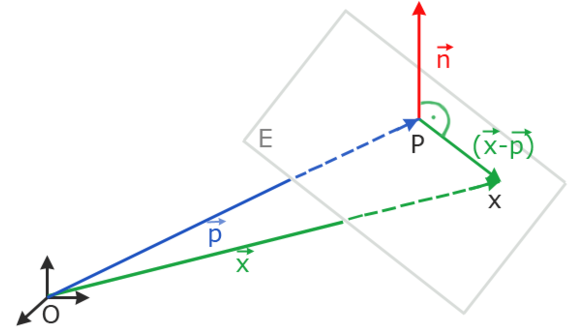
\includegraphics[width=\textwidth]{../Mathematik_1/Bilder/vektoren_ebene_normalenform.png}
\end{minipage}
	\begin{minipage}{0.55\textwidth}
\( \langle \left( \boldsymbol x - \boldsymbol p \right), \boldsymbol n \rangle = 0 \) bedeutet geometrisch,
		\begin{itemize}
			\item dass alle Vektoren \(\boldsymbol x - \boldsymbol p\) senkrecht zu dem Vektor \(\boldsymbol n\) liegen.
			\item dass alle Vektoren der Form \(\boldsymbol x -\boldsymbol p\) komplett in einer Ebene liegen (\(\boldsymbol p\) ist der Aufh�ngepunkt der Ebene).
			\item dass die Vektoren \(\boldsymbol x\) gerade die Raumpunkte sind, die zu der Ebene geh�ren. 
\end{itemize}
\end{minipage}
Eine Ebene in \(\mathbb R^3\) ist also die Angabe eines Aufh�ngepunkts und eines Normalenvektors eindeutig bestimmt. \[ E= \left\{ \boldsymbol x\in \mathbb R^3: \quad \langle \boldsymbol x- \boldsymbol p, \boldsymbol n\rangle = 0 \right\}\,.\]
\item[(b)] 
	\begin{minipage}{0.40\textwidth}
	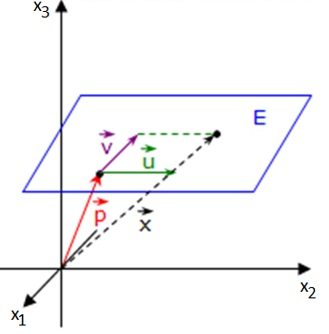
\includegraphics[width=\textwidth]{../Mathematik_1/Bilder/vektoren_ebene_parameterdarstellung.png}
\end{minipage}
	\begin{minipage}{0.55\textwidth}
		\begin{itemize}
            \item \textbf{Die abgebildete Ebene ist kein Vektorraum:}
            Sie geht nicht durch den Ursprung und enth�lt deshalb den
            Nullvektor nicht. Damit fehlt das neutrale Element der �blichen
            Vektoraddition.
            \item Die Vektoren \(\boldsymbol u\) und \(\boldsymbol v\) sind
            Richtungsvektoren der Ebene. F�r die dargestellte Ebene gilt
            \[
            E=\boldsymbol p+\mathrm{LH}\{\boldsymbol u,\boldsymbol v\}.
            \]
            \item Allgemein ist \(E\) genau dann ein Untervektorraum von
            \(\mathbb R^3\), wenn
            \[
            \boldsymbol 0\in E
            \quad\Longleftrightarrow\quad
            \langle\boldsymbol p,\boldsymbol n\rangle=0.
            \]
            Dann geht die Ebene durch den Ursprung, hat Dimension zwei und
            zwei linear unabh�ngige Richtungsvektoren bilden eine Basis.
\end{itemize}
\end{minipage}
\end{itemize}
\end{exercisebox}

\begin{exercisebox}[Basis]
		Gegeben sei der Vektor \( \boldsymbol a^\intercal = \left( \sqrt{3}, 1\right)^\intercal\). Bestimmen Sie zwei Vektoren \(\boldsymbol  v\) und \(\boldsymbol w\), die eine Orthonormalbasis des \(\mathbb R^2\) sind und \(\boldsymbol v \parallel \boldsymbol a\).
		\vspace{0.2cm}
	\noindent\textbf{L�sung:}\newline
	Merken Sie sich: zu gegebenen Vektor in \(\mathbb R^2\) ist ein senkrechter Vektor einfach zu bestimmen: man dreht einfach die Koeffizienten um und f�gt zu einem ein Minuszeichen hinzu:\marginnote{Nur \(\mathbb R^2\)}   
	\[ \forall\; x_1, x_2 \in \mathbb R:\quad  \left(\begin{array}{c} x_1 \\x_2 \end{array} \right) \perp \left( \begin{array}{c} -x_2 \\x_1\end{array}\right) \]
	Und damit l�sen wir die Aufgabe in zwei Schritten:
	\begin{enumerate} 
		\item Normierung des Vektors \(\boldsymbol a\) liefert den ersten Basisvektor: \[ \hat {\boldsymbol e}_2 = \dfrac{1}{\sqrt{ (\sqrt{3})^2 + 1^2} } \left( \begin{array}{c} \sqrt{3} \\ 1\end{array}\right) = \dfrac12 \left( \begin{array}{c} \sqrt{3} \\ 1\end{array}\right) \,.\]
		\item Bestimmung eines normierten Vektors, der zu \(\boldsymbol a\) senkrecht ist: \[ \boldsymbol e_2 = \left( \begin{array}{c}-1 \\  \sqrt{3} \end{array}\right) \Rightarrow \hat{ \boldsymbol e}_2 = \dfrac{1}{2}\left( \begin{array}{c}-1 \\  \sqrt{3} \end{array}\right)\,.\]
	\end{enumerate}
\end{exercisebox}

\begin{exercisebox}[Dimension]
	Welche Dimension haben die folgenden reellen Vektorr�ume?
	\begin{itemize}
		\item[(a)] $ \mathbb V_1 = \left\{ \boldsymbol x \in \mathbb R^n: \boldsymbol x = \alpha \boldsymbol a\,, \; \boldsymbol a \in \mathbb R^n\setminus\{\boldsymbol 0\} \right\} $
		\item[(b)] $ \mathbb V_2 = \left\{ \boldsymbol x \in \mathbb R^3: \boldsymbol x = \alpha \boldsymbol a + \beta \boldsymbol b\,, \; \boldsymbol b,\boldsymbol a \in \mathbb R^3\setminus\{ \boldsymbol 0 \}, \; \boldsymbol a \times \boldsymbol b =0 \right\}$
	\end{itemize}

\noindent \textbf{L�sung:}
	\begin{itemize}
		\item[(a)] Die Menge $M_1:=\left\{ \boldsymbol x \in \mathbb R^n: \boldsymbol x = \alpha \boldsymbol a\,, \; \boldsymbol a \in \mathbb R^n\setminus\{\boldsymbol 0\}\right\}$ beschreibt eine Gerade im Raum, die durch den Ursprung verl�uft. Es gibt einen frei w�hlbaren Parameter, also gilt $\mathrm{dim}M = 1$.
		\item[(b)] Die Menge $M_2:=\left\{ \boldsymbol x \in \mathbb R^3: \boldsymbol x = \alpha \boldsymbol a + \beta \boldsymbol b\,, \; \boldsymbol a, \boldsymbol b \in \mathbb R^3\setminus\{\boldsymbol 0\}, \boldsymbol a\times \boldsymbol b = 0\right\}$ beschreibt dieselbe Gerade wie die Menge $M_1$ und hat damit auch Dimension eins. Da die Vektoren $\boldsymbol a$ und $\boldsymbol b$ parallel zueinander sind, gilt \[ \boldsymbol x = \alpha \boldsymbol a + \beta \boldsymbol b = \alpha \boldsymbol a + \beta (\lambda \boldsymbol a) = \underbrace{(\alpha + \beta\cdot \lambda)}_{\displaystyle{=t}} \boldsymbol a\] 
				Bemerkung: w�ren die Vektoren $\boldsymbol a$ und $\boldsymbol b$ linear unabh�ngig, dann w�re $M_2$ eine Ebene im Raum mit Dimension zwei.
	\end{itemize}
\end{exercisebox}

\begin{exercisebox}[Anwendung: Krummlinige Koordinaten]
	\begin{itemize}
		\item[(a)] Bestimmen Sie die Polarkoordinaten eines beliebigen Vektors \(\boldsymbol x \in \mathbb R^2\setminus \{\boldsymbol 0\}\).
		\item[(b)] Zeigen Sie, dass  die Vektoren \[ \boldsymbol e_{\varphi} = \left( \begin{array}{c} -\sin(\varphi) \\\cos(\varphi) \end{array}\right), \; \boldsymbol e_{r} = \left( \begin{array}{c} \cos(\varphi) \\\sin(\varphi) \end{array}\right) \; \textnormal{mit}\; r\in [0,\infty), \; \varphi\in (-\frac{\pi}{2}, \frac{\pi}{2}] \] eine Orthonormalbasis des \(\mathbb R^2\) sind.
			\item[(c)] Skizzieren Sie f�r \(r=1\) und \(\varphi = \pi/4\) die Orthonormalbasen \( \{\boldsymbol e_x, \boldsymbol e_y\}  \) und \( \{\boldsymbol e_r, \boldsymbol e_\varphi\}  \) in einem gemeinsamen Koordinatensystem.  
	\end{itemize}
\noindent \textbf{L�sung:}
	\begin{itemize}
		\item[(a)] Die kartesischen Koordinaten von \(\boldsymbol x\) seien \(x_1\) und \(x_2\), also \( \boldsymbol x \widehat = (x_1, x_2\). Die Polarkoordinaten \( (r, \varphi)\) lauten \[ (r, \varphi) = ( \sqrt{ x_1^2 + x_2^2} , \mathrm{atan2}\left(x_2, x_1\right) \] 
				\item[(b)] Zu zeigen ist, dass die Vektoren aufeinander senkrecht stehen (Skalarprodukt!) und jeweils die Norm eins besitzten, also 
					\begin{eqnarray*} \langle \boldsymbol e_\varphi, \boldsymbol e_r\rangle &=& -\sin(\varphi) \cdot \cos(\varphi) + \cos(\varphi) \cdot \sin(\varphi) = 0\,,\\ 
						|\boldsymbol e_\varphi| &=& \sqrt{ (-\sin(\varphi))^2 + (\cos(\varphi))^2} =  \sqrt{1} = 1\,,\\ 
						|\boldsymbol e_r| &=& \sqrt{ (\cos(\varphi))^2 + (\sin(\varphi))^2} =  \sqrt{1} = 1\,. 
					\end{eqnarray*}
				\item[(c)] 
	\begin{minipage}{0.45\textwidth}
	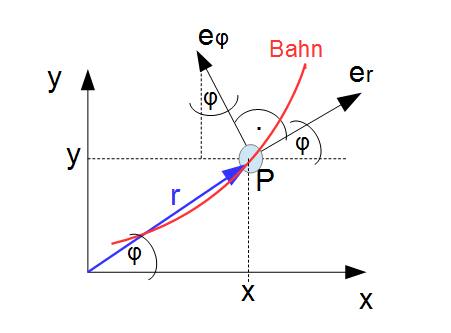
\includegraphics[width=\textwidth]{../Mathematik_1/Bilder/vektoren_polarbasis_bahnkurve.png}
\end{minipage}
	\begin{minipage}{0.55\textwidth}
		\begin{itemize}
			\item Der Vektor \(\boldsymbol e_r\) ist parallel zum Ortsvektor \(\boldsymbol P\).
			\item Der Vektor \(\boldsymbol e_\varphi\) ist senkrecht zum Ortsvektor \(\boldsymbol P\).
	\end{itemize}
\end{minipage}
					
\textbf{Bemerkung:} Die Polarbasis richtet sich nach dem Ortsvektor:
\(\boldsymbol e_r\) zeigt radial vom Ursprung zum Punkt,
\(\boldsymbol e_\varphi\) steht dazu senkrecht und zeigt in Richtung
zunehmenden Winkels. Diese Richtungen stimmen im Allgemeinen nicht mit der
Tangential- und Normalenrichtung einer Bahnkurve �berein. Bei einer
Kreisbahn um den Ursprung ist \(\boldsymbol e_\varphi\) tangential und
\(\boldsymbol e_r\) radial nach au�en gerichtet; die nach innen gerichtete
Normale ist dann \(-\boldsymbol e_r\). Die Polarbasis h�ngt vom Winkel
\(\varphi\) ab und �ndert sich entlang einer Bahn nur dann, wenn sich dieser
Winkel �ndert.
	\end{itemize}
\end{exercisebox}
\begin{exercisebox}[Analytische Geometrie]
	Es sei $\boldsymbol r, \boldsymbol n\in\mathbb R^3$. Welches geometrische Objekt stellt die L�sungsmenge der folgenden Gleichung(en) dar? 
	\[ \boldsymbol x \in \mathbb R^3: \; \left( \boldsymbol x - \boldsymbol r \right) \boldsymbol \cdot \boldsymbol n = 0\]

	\vspace{0.3cm}
	\noindent\textbf{L�sung:}\newline
	Ebene mit Aufh�ngepunkt $\boldsymbol r$ und Normale $\boldsymbol n$.
\end{exercisebox}

\begin{exercisebox}[Lineare Funktion]
	Wie l��t sich eine Funktion $f:\mathbb R^n \to \mathbb R$ beschreiben, die in jedem Argument linear ist? Es gelte also \[ f( x_1, x_2, \dots, \alpha x_i, \dots, x_n) = \alpha f(x_1,x_2,\dots, x_i, \dots, x_n)\quad i=1,\dots,n\,.\]

	\vspace{0.3cm}
	\noindent\textbf{L�sung:}\newline
	Um eine Abbildungsvorschrift f�r $f$ zu bekommen, ist es geschickt sich zu �berlegen, wie $f$ mit nur einem Argument umgeht. Was macht die Anwendung von $f$ aus dem Vektor $\boldsymbol x_i: = (0,0,\dots,0,x_i,0,\dots,0)^\intercal$? Laut Voraussetzung ist das Bild dieser Anwendung linear von $x_i$ abh�ngig, also  \[ f( \boldsymbol x_i) = a_i x_i \quad \textnormal{mit}\; a_i \in \mathbb R\,. \] Dieses Verhalten gilt in jedem Argument, also $i=1,\dots,n$ \[ f: \mathbb R^n \to \mathbb R, \boldsymbol x \mapsto f(\boldsymbol x) = a_1 x_1 +  a_2 x_2 + \dots + a_nx_n =  \sum\limits_{i=1}^{n}a_i x_i = \langle \boldsymbol a, \boldsymbol x\rangle \quad \textnormal{mit}\; \boldsymbol a\in \mathbb R^n\,.\]
\end{exercisebox}

\begin{exercisebox}[Tangenten]
	Gegeben ist die Funktion $f: \mathbb R \to \mathbb R, \; x\mapsto \frac14 x^2$. Ihr Graph sei $K$. 
  \begin{enumerate}
    \item Zeigen Sie, dass die Tangenten an $K$ in den Punkten $B_1\left(-3|\frac94\right)$ und  $B_2\left(\frac43|\frac49\right)$ orthogonal zueinander sind. Zeichnen Sie $K$ zusammen mit diesen Tangenten. 
    \item Es seien $S_1\left(a|f(a)\right)$ und  $S_2\left(b|f(b)\right)$ Punkte auf $K$. Welche Beziehung besteht zwischen $a$ und $b$, wenn die Tangenten an $K$ in $S_1$ und $S_2$ orthogonal sind?
    \item Bestimmen Sie die Punkte  $S_1\left(a|f(a)\right)$ und  $S_2\left(b|f(b)\right)$ so, dass die Tangenten in $S_1$ und $S_2$ orthogonal zueinander sind und die Strecke $S_1S_2$ parallel zur $x$-Achse ist. 
  \end{enumerate}

	\vspace{0.3cm}
	\noindent\textbf{L�sung:}\newline
	\begin{enumerate}
		\item Es gilt  $f'(x) = \frac12 x$. Also besitzen die  Tangenten in den Punkten $B_1$ und $B_2$ die Gleichungen 
			\begin{eqnarray*} 
				t_1(x) &=& f'(-3)(x + 3) + \frac94 =-\frac32 (x+3) + \frac94\,, \\
				t_2(x) &=& f'(\frac43)(x + \frac43) + \frac49 =\frac23 (x+ \frac43) + \frac49\,.
			\end{eqnarray*}
			Mit Hilfe zweier beliebiger Punkte auf den Gerade kann man die Richtungsvektoren ausrechnen  \begin{eqnarray*} 
				\boldsymbol r_1 &=& \left(\begin{array}{c} -3 \\ \frac94\end{array} \right) - \left(\begin{array}{c}0\\ -\frac94\end{array}\right) = \left( \begin{array}{c} -3 \\ \frac{9}{2} \end{array}\right)\,,\\
				\boldsymbol r_2 &=& \left(\begin{array}{c} \frac43 \\ \frac49\end{array} \right) - \left(\begin{array}{c}0\\ -\frac49\end{array}\right) = \left( \begin{array}{c} \frac43 \\ \frac89 \end{array}\right)\,.
			\end{eqnarray*}
			Die Tangenten stehen senkrecht aufeinander, da das Skalarprodukts zwischen $\boldsymbol r_1 $ und $\boldsymbol r_2$ verschwindet:
			\[ \boldsymbol r_1 \boldsymbol \cdot \boldsymbol r_2 = \left(\begin{array}{c} \frac43 \\ \frac89\end{array} \right)\boldsymbol \cdot \left(\begin{array}{c} -3 \\ \frac92\end{array} \right) = \frac43\cdot (-3) + \frac89 \cdot \frac92 = -4 + 4 = 0\,.\]
			Bemerkung: alternativ kann man das Produkt der Steigungen �berpr�fen. Es gilt $f'(-3)\cdot f'(\frac43)=-1$, d.h. die Tangenten in $B_1$ und $B_2$ sind orthogonal. 
		\item Wegen $f'(a) = \frac12 a $ und $f'(b) = \frac12 b$ folgt aus $f'(a) \cdot f'(b) = -1 $ die gesuchte BEziehung $a\cdot b = -4$.
		\item $\overline{S_1S_2} $ ist parallel zur $x$-Achse, wenn $f(a) = f(b)$ gilt, also $\frac14 a^2 = \frac14 b^2$ und damit $a^2=b^2$ Mit $a\cdot b = -4$ aus dem zweiten Aufgabenteil erh�lt man $S_1(2|1)$ und $S_2(-2|1)$.
	\end{enumerate}
\end{exercisebox}

\begin{exercisebox}[Tangenten]
  \begin{enumerate}
	  \item Gegeben ist die Funktion \[ f: \mathbb R \to \mathbb R, x \mapsto \frac14 x^2 + cx\,.\] 
		  Der Graph von $f$ schneidet die $x$-Achse im Ursprung $O(0|0)$ und im Punkt $A(a|0)$. Die Tangenten an den Graphen in $O$ und $A$ schneiden sich im Punkt $B$. Zeigen Sie, dass das Dreieck $OAB$ stets gleichschenklig ist. Bestimmen Sie den Koeffizienten $c$ so, dass das Dreieck $OAB$ auch rechtwinklig ist.
	  \item Gegeben ist die Funktion \[ g: \mathbb R \to \mathbb R, \; x \mapsto 2 \sin(cx), \quad c \in (0,\infty)\,. \] Der Graph von $g$ schneidet die $x$-Achse im Ursprung $O=(0|0)$ und im Punkt $A(\frac{\pi}{c}|0)$. Die Tangenten an den Graphen in $O$ und $A$ schneiden sich im Punkt $B$. Bestimmen Sie den Koeffizienten $c$ so, dass das Dreieck $OAB$ gleichseitig ist. 
  \end{enumerate}

	\vspace{0.3cm}
	\noindent\textbf{L�sung:}\newline
	\begin{enumerate}
		\item Es ist $a=-4c$ und $f'(x) = \frac12+c$. Die Tangentengleichungen in den Punkten $O$ und $A$ und der Schnittpunkt $B$ lauten 
			\begin{eqnarray*}
				t_1(x) &=& f'(0)x = cx \\ t_2(x) &=& f'(a) (x-a) = (\frac12 \cdot (-4c) + c) (x-a) = -c (x-a)\\
				t_1(x) &=& t_2(x) \Leftrightarrow x = \frac12 ca  \Rightarrow B(\frac12 a| \frac12 c a)
			\end{eqnarray*}
			Die $x$-Koordinate von $B$ teilt gerade die Strecke $OA$. Damit ist das Dreieck gleichschenklig. Damit as Dreieck rechtwinklig ist, muss $c$ so eingerichtet werden, dass die Tangenten im Punkt $B$ senkrecht aufeinander stehen. Die Richtungsvektoren lauten:
			\begin{eqnarray*}
				\boldsymbol r_2 =\left( \begin{array}{c} a - \frac12 a \\ -\frac12 ca \end{array}\right)  \quad \textnormal{und} \quad 
				\boldsymbol r_1 =\left( \begin{array}{c} \frac12 a \\ \frac12 ca \end{array}\right) 
			\end{eqnarray*}
			Also gilt   $\boldsymbol r_1 \boldsymbol \cdot \boldsymbol r_2 = 0$ genau dann, wenn $\frac14 a^2 - \frac14 c^2 a^2 = 0 \Leftrightarrow c= 1\,.$ 
		\item Es ist $f'(x) = 2c\cdot \cos(cx)$. 
		Die Tangentengleichungen in den Punkten $O$ und $A$ und der Schnittpunkt $B$ lauten 
			\begin{eqnarray*}
				t_1(x) &=& f'(0)x = 2c x \\ t_2(x) &=& f'(\frac{\pi}{2}) (x-\frac{\pi}{2}) = -2c (x-\frac{\pi}{c})\\
				t_1(x) &=& t_2(x) \Leftrightarrow cx = -2c(x-\frac{\pi}{c})  \Rightarrow B(\frac{\pi}{2c}| \pi)
			\end{eqnarray*}
			Die $x$-Koordinate von $B$ teilt gerade die Strecke $OA$. Damit ist das Dreieck gleichschenklig. Das Dreieck ist gleichseitig, wenn alle Winkel im Dreieck $\frac23\pi \widehat = 60^\circ$ betragen, d.h. \[ \tan(\frac23\pi) = \sqrt{3} \stackrel{!}{=} \frac{\pi}{\frac{\pi}{2c}} \Rightarrow c = \frac12\sqrt{3}\]
	\end{enumerate}
\end{exercisebox}

 \newpage 
\setcounter{exercise}{0}\pagestyle{empty} \section*{Matrizen L�sungen}\label{MA1-matrizen-loesungen}

\ifintegriereaufgaben
	Regeln und Beispiele, die zum Verst�ndnis der L�sungswege hilfreich sind, finden Sie im Skript\wennreferenzvorhanden{MA1-matrizen}{ (Abschnitt \abschnittsverweis{MA1-matrizen})}.
\else
	Regeln und Beispiele, die zum Verst�ndnis der L�sungswege hilfreich sind, finden Sie im Skript.
\fi 

\begin{exercisebox}[Rechenregeln]
	Gegeben seien die Matrizen 
	\[ A = \left( \begin{array}{ccc} 1 & -2 & 3 \\ 0 & 3 & 1 \end{array}\right), \quad B = \left( \begin{array}{cc} 2 & -1 \\ 0 & 3 \\ -2 & -2 \end{array}\right), \quad C=\left( \begin{array}{cc} 3 & 2 \\ -1 & 2 \end{array}\right) \,. \]
	Berechnen Sie $ ( A^\intercal C - 2\cdot B)(-3\cdot C^\intercal )\,.$

\vspace{0.3cm}
\noindent\textbf{L�sung:}\newline
\[ \left( \begin{array}{cc} -15 & -27 \\ 105 & -3 \\ -180 & -36 \end{array}\right)\,. \]
\end{exercisebox}

%\begin{exercisebox}[Matrixmultiplikation und Skalarprodukt]
%Es sei $\boldsymbol a \in \mathbb R^n, \boldsymbol b\in \mathbb R^m$ und $A\in \mathbb R^{n\times m}$.  Zeigen Sie $\langle \boldsymbol a , A \boldsymbol b\rangle = \langle A^\intercal \boldsymbol a, \boldsymbol b \rangle\,.$
%
%\vspace{0.3cm}
%\noindent\textbf{L�sung:}\newline
%\begin{eqnarray*}
%	\langle \boldsymbol a, A\boldsymbol b\rangle &=& \sum\limits_{i=1}^n \left( a_i \cdot \left( A \boldsymbol b\right)_i \right) \\
%	&=& \sum\limits_{i=1}^n a_i \left( \sum\limits_{j}^m a_{ij} b_j \right) \\
%	&=& \sum\limits_{i=1}^n\sum\limits_{j}^m  a_i a_{ij} b_j  \\
%	&=&  \sum\limits_{j}^m \left(\sum\limits_{i=1}^n  \underbrace{a_i a_{ij}}_{\displaystyle{= \boldsymbol a^\intercal A = \left( \boldsymbol a A^\intercal \right)^\intercal = \boldsymbol a A^\intercal }} \right) b_j  \\
%	&=&  \sum\limits_{j}^m \left(A^\intercal \boldsymbol a \right)_j b_j
%\end{eqnarray*}
%\end{exercisebox}

\begin{exercisebox}[Rang und Bild]
	Es sei $A = \boldsymbol a \boldsymbol b^\intercal, \quad \boldsymbol a \in \mathbb R^n, \boldsymbol b \in \mathbb R^m$. Wie ist der Rang der Matrix $A$? Wie sieht das Bild der Matrix aus?


\vspace{0.3cm}
\noindent\textbf{L�sung:}\newline
Der Rang der Matrix $A \in \mathbb R^{n\times m}$ entspricht der Dimension des Bildes der linearen Abbildung $A:\mathbb R^m \to \mathbb R^n$. Es gilt 
\begin{eqnarray*} 
	\forall \boldsymbol y \in \mathbb R^m: A\boldsymbol y &=& (\boldsymbol a \boldsymbol b^\intercal) \boldsymbol y = \boldsymbol a \underbrace{(\boldsymbol b^\intercal  \boldsymbol y)}_{\displaystyle{ =: \lambda \in \mathbb R!}} = \lambda \boldsymbol a\,,
\end{eqnarray*}
wobei wir das Assoziativgesetz der Matrixmultiplikation, $(A B)C = A(BC)$, ausgenutzt haben. Die Multiplikation eines Zeilenvektors mit einem Spaltenvektor gleicher Gr��e ist eine reelle Zahl\footnote{ im Grunde ist diese Zahl das Skalarprodukt der beiden Vektoren: \(
\boldsymbol b^\intercal  \boldsymbol y = \langle \boldsymbol b ,\boldsymbol y\rangle =:  \lambda \in \mathbb R\,. \)}
Damit umfasst das Bild der linearen Abbildung $A$ alle skalaren Vielfachen des Vektors $\boldsymbol a$ und damit
\[ \mathrm{rk}(A) = \mathrm{dim}\left( \mathrm{im}A\right) = \mathrm{dim} \{ \boldsymbol x \in \mathbb R^n: \boldsymbol x = \lambda \boldsymbol a\} = 1\,.\]
\end{exercisebox}

\begin{exercisebox}[Basis]
	\begin{itemize}
		\item[(a)] F�r welche Werte von $a\in\mathbb R$ bilden die vier Vektoren eine Basis des $\mathbb R^4$?
  \begin{eqnarray*}
	  \boldsymbol x_1 = (3,1,4,0)^\intercal, \;  
	  \boldsymbol x_2 = (1,1,0,6)^\intercal, \; 
	  \boldsymbol x_3 = (-4,0,5,a)^\intercal, \;  
	  \boldsymbol x_4 = (0,0,1,2)^\intercal\,.
  \end{eqnarray*}

\item[(b)]	  �berpr�fen Sie, ob die Polynome $1, 1+x, 1-x, x^2$ eine Basis des $\mathcal P_2$ bilden.
\end{itemize}

  %\hspace{0.3cm}
  %\newline
  \textbf{L�sung:}
 \begin{itemize}
	 \item[(a)] Die Vektoren sind genau dann linear unabh�ngig, wenn die Matrix
		 \[ A_a := \left( \begin{array}{cccc} 3 & 1 & -4 & 0 \\ 1 & 1 & 0 & 0 \\ 4 & 0 & 5 & 1 \\ 0 & 6 & a & 2 \end{array}\right) \in \mathbb R^{4\times 4}\,, \]
		 
		 deren Spalten $\boldsymbol x_1, \boldsymbol x_2, \boldsymbol x_3$ und $\boldsymbol x_4$ sind, vollen Rang hat. Wir bringen $A_a$ auf Dreiecksform und bestimmen den Rang in Abh�ngigkeit von $a\in \mathbb R$. Es ist geschickt die zwei letzten Spalten zu vertauschen, so dass der Parameter \(a\) rechts unten landet und so in m�glichst wenig Rechenoperationen mitgeschleppt wird:      
		 \begin{eqnarray*}
			 \left( \begin{array}{cccc} 3 & 1 & -4 & 0 \\ 1 & 1 & 0 & 0 \\ 4 & 0 & 5 & 1 \\ 0 & 6 & a & 2 \end{array}\right) &\Leftrightarrow&
			 \left( \begin{array}{cccc} 3 & 1 & 0 & -4 \\ 1 & 1 & 0 & 0 \\ 4 & 0 & 1 & 5 \\ 0 & 6 & 2 & a \end{array}\right) \Leftrightarrow 
		 \left( \begin{array}{cccc} 3 & 1 & 0 & -4 \\ 0 & -2 & 0 & -4 \\ 0 & 4 & -3 & -31 \\ 0 & 6 & 2 & a \end{array}\right) \\
		 \left( \begin{array}{cccc} 3 & 1 & 0 & -4 \\ 0 & -2 & 0 & -4 \\ 0 & 0 & -3 & -39 \\ 0 & 0 & 2 & -12+a \end{array}\right) &\Leftrightarrow& 
		 \left( \begin{array}{cccc} 3 & 1 & 0 & -4 \\ 0 & -2 & 0 & -4 \\ 0 & 0 & -3 & -39 \\ 0 & 0 & 0 & -114-3a \end{array}\right) \,.
	 \end{eqnarray*}
	 F�r $a=38$ hat die Matrix $A_{38}$ also Rang $3<4$ beliebig und damit sind die Vektoren f�r $a=38$ linear abh�ngig. F�r $a\not = 38$ hat die Matrix vollen Rang und das hei�t die Vektoren sind linear unabh�ngig.
 \item[(b)]
	 Zwei L�sungsvarianten: 
	 \begin{itemize}
		 \item Die drei Polynome \(\{p_0(x)= 1, p_1(x)= 1+x, P_2(x)= 1-x\}\) sind linear abh�ngig, weil \[ p_0(x) = \frac12 p_1(x) + \frac12 p_2(x)\,.\] Also kann es sich nicht um eine Basis handeln.  
		 \item Der systematische Weg zu pr�fen, ob die gegebenen Polynome linear abh�ngig sind ist folgender: man zeige, dass die Nullabbildung \(x\mapsto 0\) auf nichttriviale Weise darstellbar ist, dass also die Gleichung 
	 \[ \alpha_1 \cdot 1 + \alpha_2 \cdot (1+x) + \alpha_3 \cdot (1-x) +\alpha_4 \cdot x^2 = 0 \quad (*)\,,\]
	 mindestens eine nichttriviale L�sung besitzt. Nichttriviale L�sung hei�t, dass f�r mindestens einen Koeffizienten \(\alpha_i, i\in \{1,2,3,4\},\) gilt $\alpha_i\not= 0$. Aus $(*)$ folgt durch Ausklammern und Zusammenfassen 
	\begin{eqnarray*}
		1\cdot (\alpha_1 + \alpha_2 + \alpha_3) + x\cdot ( \alpha_2 - \alpha_3) + \alpha_4 x^2 = 0 \,,
	\end{eqnarray*}
	und hieraus folgt f�r die unbekannten Koeffizienten $\alpha_i, \; i=1,2,3,4$:
	\begin{eqnarray*}
		\left\{ \begin{array}{lcl}
		\alpha_1 + \alpha_2 + \alpha_3 &=& 0 \\
		\alpha_2 - \alpha_3 &=& 0\\
\alpha_4 &=& 0 
\end{array}\right.
\end{eqnarray*}
Dieses Gleichungssystem ist unterbestimmt und hat unendlich viele L�sungen:
\begin{eqnarray*}
	\Rightarrow \begin{cases}{r}  \alpha_1 = -2t \\ \alpha_2=\alpha_3=t\in \mathbb R  \\ \alpha_4 = 0\,.
	\end{cases}
\end{eqnarray*}
Die Polynome $1, 1+x, 1-x, x^2$ bilden also kein minimales Erzeugendensystem, sind also keine Basis des $\mathcal P_2$. Zum Beispiel erhalten wir f�r $t=1$ die Koeffizienten $\alpha_1 = -2, \alpha_2=1, \alpha_3=1, \alpha_4 =0$, die eine nichttriviale Linearkombination bilden. 
\end{itemize}
\end{itemize}
\end{exercisebox}

\begin{exercisebox}[Lineare Abbildungen]
	Gegeben sind die linearen Abbildungen 
	\[ \mathcal A: \mathbb R^2 \to \mathbb R^3, \left( \begin{array}{c} x_1 \\ x_2 \end{array}\right) \mapsto \left( \begin{array}{c} 0 \\ 3x_1-x_2 \\ 2x_2 \end{array}\right), \quad \mathcal B:\mathbb R^2 \to \mathbb R^3, \left( \begin{array}{c} x_1 \\ x_2 \end{array}\right) \mapsto \left( \begin{array}{c} -x_1+x_2 \\ -x_2 \\ 3x_2 \end{array}\right)\,.\]
	\begin{itemize}
		\item[(a)] Bestimmen Sie die darstellenden Matrizen $A$ und $B$ der linearen Abbildungen $\mathcal A$ und $\mathcal B$.
		\item[(b)] Gegeben ist eine Matrix \[ C=\left( \begin{array}{ccc} -1 & 2 & 0 \\ 0 & 3 & -1 \end{array}\right) \in \mathbb R^{2\times 3}\] Bestimmen SIe die von $C$ induzierte lineare Abbildung $\mathcal C$.
		\item[(c)] Wie lautet die darstellende Matrix der linearen Abbildung $\mathcal C\circ \mathcal A$?
	\end{itemize}

\vspace{0.3cm}
\noindent\textbf{L�sung:}\newline
\begin{itemize}
	\item[(a)] Die darstellenden Matrizen sind 
		\[ A = \left( \begin{array}{cc} 0 & 0 \\ 3 & -1 \\ 0 & 2 \end{array} \right), \quad B=\left( \begin{array}{cc} -1 & 1 \\ 0 & -1 \\ 0 & 3 \end{array}\right) \,. \]
	\item[(b)] Die Abbildung ist durch \[ \mathcal C:\mathbb R^3 \to \mathbb R^2, \quad \left( \begin{array}{c} x_1 \\x_2 \\x_3\end{array}\right) \mapsto \left( \begin{array}{ccc} -1 & 2 & 0 \\ 0 & 3 & -1 \end{array}\right) \left( \begin{array}{c} x_1 \\x_2 \\x_3\end{array}\right) = \left( \begin{array}{c} -x_1 + 2 x_2 \\3x_2 - x_3 \end{array}\right) \] gegeben. 
	\item[(c)] Es gilt \[ M_{\mathcal C \circ  \mathcal B} = CB= \left( \begin{array}{ccc} -1 & 2 & 0 \\ 0 & 3 & -1 \end{array}\right) \left( \begin{array}{cc} -1 & 1 \\ 0 & -1 \\ 0 & 3 \end{array}\right) =  \left( \begin{array}{cc} 6 & -2 \\ 9 & -5 \end{array}\right)\,.\]
\end{itemize}
\end{exercisebox}

\begin{exercisebox}[Lineare Abbildungen]
	Gegeben sei der reelle Vektorraum 
	\[ \mathcal P_3:= \left\{ p:\mathbb R\to \mathbb R\;|\;p \;\textnormal{Polynome vom Grad } 3\right\}\] und die Abbildung \[ f: \mathcal P_3 \to \mathbb R^2, \quad p\mapsto \left( \begin{array}{c}p(2) \\ p(3)\end{array}\right) \,.\]
	\begin{itemize}
		\item[(a)] Zeigen Sie, dass $f$ eine lineare Abbildung ist und berechnen Sie $f$ f�r die Monome $p_i: x\mapsto x^i,\; i=0,1,2,3\,.$
		\item[(b)] Berechnen Sie $f(p)$ f�r ein allgemeines Polynom $p \in \mathcal P_4$. % mit  \[ p=a_3\cdot p_3 + a_2 \cdot p_2 + a_1\cdot p_1 + a_0 \cdot p_0, \quad a_0,\dots,a_3\in \mathbb R.\] 
		\item[(d)] Zeigen Sie, dass die Funktion \[ g:\mathbb R^4 \to \mathbb R^2, \quad \left( \begin{array}{c}a_3 \\ a_2 \\ a_1 \\ a_0\end{array}\right) \mapsto f(a_3\cdot p_3 + a_2 \cdot p_2 + a_1\cdot p_1 + a_0 \cdot p_0)\] linear ist und berechnen Sie die darstellende Matrix von $g$.
	\end{itemize}

\vspace{0.3cm}
\noindent\textbf{L�sung:}\newline
\begin{itemize}
	\item[(a)] Es gilt f�r $p, q \in \Pi_3$ und $\lambda \in \mathbb R$
		\begin{eqnarray*}
			f(p + q) &=& \left( \begin{array}{c} (p+q) (2) \\ (p + q)(3) \end{array}\right) =  \left( \begin{array}{c} p(2) + q(2) \\ p(3) + q(3) \end{array}\right) =\left( \begin{array}{c} p(2)\\ p(3) \end{array}\right) + \left( \begin{array}{c} q(2) \\ q(3) \end{array}\right) =  f(p) + f(q)\,, \\[1ex]
	f(\lambda \cdot p) &=& \left( \begin{array}{c} \lambda \cdot p(2) \\ \lambda \cdot p(3) \end{array}\right) =  \lambda \cdot \left( \begin{array}{c} p(2) \\ p(3) \end{array}\right) = \lambda \cdot f(p) \,. 
\end{eqnarray*}
Es gilt 
	\[ 
	f(p_0) = \left( \begin{array}{c} 1 \\1 \end{array}\right), \; 
	f(p_1) = \left( \begin{array}{c} 2 \\3 \end{array}\right), \; 
	f(p_2) = \left( \begin{array}{c} 4 \\9 \end{array}\right), \; 
	f(p_3) = \left( \begin{array}{c} 8 \\27 \end{array}\right)\,.
 \]
\item[(b)] Durch die Linearit�t folgt 
	\begin{eqnarray*} 
		f(p) &=& f(a_3\cdot p_3 + a_2\cdot p_2 + a_1\cdot p_1 + a_0\cdot p_0) \\
	&=& a_3  f(p_3) + a_2 f(p_2) + a_1 f(p_1) + a_0f(p_0) \\
	&\stackrel{(b)}{=}&  \left( \begin{array}{c} 8a_3 + 4a_2 + 2a_1 + a_0 \\ 27a_3 + 9a_2 + 3a_1 + a_0 \end{array}\right) 
\end{eqnarray*}
\item[(c)] Es gilt 
	\[ g: \mathbb R^4 \to \mathbb R^2, \quad \left( \begin{array}{c} a_3 \\ a_2 \\ a_1 \\ a_0 \end{array}\right) \mapsto \left( \begin{array}{c} 8a_3 + 4a_2 + 2a_1 + a_0 \\ 27a_3 + 9a_2 + 3a_1 + a_0 \end{array}\right)	
	\]
		Damit ist die darstellende Matrix durch 
		\[ M_g = \left( \begin{array}{cccc} 8 & 4 & 2 &1 \\ 27 & 9 & 3 & 1 \end{array}\right) \]
		gegeben und es gilt 
		\[ g( \boldsymbol a ) = \left( \begin{array}{cccc} 8 & 4 & 2 &1 \\ 27 & 9 & 3 & 1 \end{array}\right) \boldsymbol a \,. \]
\end{itemize}

\end{exercisebox}

 \newpage 
\setcounter{exercise}{0}\pagestyle{empty} \section*{Lineare Gleichungssysteme L�sungen}\label{MA1-lineare-gleichungssysteme-loesungen}

\ifintegriereaufgaben
	Regeln und Beispiele, die zum Verst�ndnis der L�sungswege hilfreich sind, finden Sie im Skript\wennreferenzvorhanden{MA1-lineare-gleichungssysteme}{ (Abschnitt \abschnittsverweis{MA1-lineare-gleichungssysteme})}.
\else
	Regeln und Beispiele, die zum Verst�ndnis der L�sungswege hilfreich sind, finden Sie im Skript.
\fi 


\begin{exercisebox}[Rechenregeln]
Wie muss $\boldsymbol b$ gew�hlt werden, dass gilt $A\boldsymbol x =\boldsymbol b$ mit 
\[ \left( \begin{array}{ccccc} -1 & 0 & 0 & 3 & -2 \\  2 & -1 & 1 & 0 & 0 \\ 1 & 1 & -1 & -2 & 0 \end{array}\right), \quad \boldsymbol x = \left( -1, 2,-2,3,5\right)^\intercal\,.\]

  \hspace{0.3cm}
  \newline
  \textbf{L�sung:}
  Zu berechnen ist die Matrix-Vektor Multiplikation
  \begin{eqnarray*}
	  \left( \begin{array}{ccccc} -1 & 0 & 0 & 3 & -2 \\  2 & -1 & 1 & 0 & 0 \\ 1 & 1 & -1 & -2 & 0 \end{array}\right) \left(\begin{array}{c} -1 \\ 2 \\ -2 \\3 \\5 \end{array} \right) 
%&=& \left( \begin{array}{c} 
% (-1)\cdot (-1) + 0\cdot 2 + 0\cdot (-2) + 3 \cdot 3 + (-2) \cdot 5 \\
% 2\cdot (-1) + (-1)\cdot 2 + 1\cdot (-2) + 0 \cdot 3 + 0 \cdot 5 \\
% 1\cdot (-1) + 1\cdot 2 + (-1)\cdot (-2) + (-2) \cdot 3 + 0 \cdot 5 \\
%  \end{array}\right) \\ 
  &=&  \left( \begin{array}{c} 0 \\ -6 \\ -3\end{array}\right) \,.
  \end{eqnarray*}
\end{exercisebox}

\begin{exercisebox}[L�sbarkeitsanalyse]
	Gegeben seien \[ A = \left( \begin{array}{cc} 1 & 1 \\ 2 & \alpha \end{array}\right), \quad \boldsymbol b = \left( \begin{array}{c} -2 \\ \beta \end{array}\right)\] mit Parametern $\alpha, \beta\in \mathbb R$. 
	\begin{itemize}
		\item[(a)] Bestimmen Sie den Rang der Matrix $A$ in Abh�ngigkeit von $\alpha$.
		\item[(b)] Bestimmen Sie den Rang der erweiterten Matrix $(A|b)$ in Abh�ngigkeit von $\alpha$ und $\beta$.
		\item[(c)] Bestimmen Sie in Abh�ngigkeit der beiden Parameter, wann das lineare Gleichugnssystem $A\boldsymbol x = \boldsymbol b$ l�sbar ist und wann es genau eine L�sung gibt.
	\end{itemize}

  \hspace{0.3cm}
  \newline
  \textbf{L�sung:}
  F�r die Bestimmung von $\mathrm{rk}(A)$ und $\mathrm{rk}(A_{\boldsymbol b}$ bringen wir die erweiterte Koeffizientenmatrix $\mathrm{rk}(A_{\boldsymbol b})$ auf Dreiecksform und lesen die gesuchten Gr��en ab: 
		  \begin{eqnarray*}
			  \left( \begin{array}{cc|c} 1 & 1 & -2 \\ 2 & \alpha & \beta \end{array}\right) \Leftrightarrow 
			  \left( \begin{array}{cc|c} 1 & 1 & -2 \\ 0 & \alpha-2 & \beta+4 \end{array}\right) \,. 
		  \end{eqnarray*}
		  \begin{itemize}
			  \item[(a)] 
				  $\mathrm{rk}(A) = \begin{cases} 1 \Leftrightarrow \alpha = 2\,,\\ 2  \Leftrightarrow \alpha \not= 2\,. \end{cases} $
		  \item[(b)] 
			  $\mathrm{rk}(A_{\boldsymbol b}) = \begin{cases} 1 \Leftrightarrow \alpha = 2 \land \beta = -4\,,\\ 2  \Leftrightarrow \alpha \not= 2 \lor \beta \not=-4\,. \end{cases}$ 
		  \item[(c)]  Um zu sehen f�r welche Werte von $\alpha$ und $\beta$ das Gleichungssystem l�sbar ist, bestimmen wir den Fall, f�r den das Gleichungssystem nicht l�sbar ist und negieren dann die Aussage:
			  \begin{eqnarray*}
				  \textnormal{Gleichungssystem nicht l\"osbar } &\Leftrightarrow& \; \alpha = 2 \land \beta \not= -4 \\ 
				  \Rightarrow \; \textnormal{Gleichungssystem l\"osbar } &\Leftrightarrow& \; \neg \left(  \alpha = 2 \land \beta \not= -4\right) \Leftrightarrow    \alpha \not= 2 \lor \beta = -4
			  \end{eqnarray*}
			  Das lineare Gleichungssystem ist eindeutig l�sbar genau dann, wenn $\mathrm{rk}(A) = \mathrm{rk}(A_b) = 2$, also falls $\alpha \not=2 $ und $\beta\not=-4$.
	  \end{itemize}
\end{exercisebox}
\begin{exercisebox}[Gleichungssysteme]
	Analysieren Sie die L�sbarkeit der folgenden Gleichungssysteme und bestimmen Sie die L�sungsmenge:
	\begin{eqnarray*}
		\begin{array}{lll} 
			(a) \; \begin{cases}
				x_1 -x_2 - x_3 &= 0\\
				x_1 +x_2 + 3x_3 &= 4\\
				     x_2 + 2x_3 &= 2\\
				     2x_1 + x_3 &= 3\\
    \end{cases} 
    &\;\;  
    (b)\; \begin{cases}
	    x_1 + x_2 - x_3 + x_4 - x_5 &= 1\\
    -x_1 + x_2 - 3 x_3 + 3x_5 &= 2\\
    x_2 - 2 x_3 + x_4 - x_5 &= -1\\
    2x_1 + 2 x_3 + x_4 - 2 x_5 &= 1
  \end{cases}
  \;\; (c)\; \begin{cases}
	x_1 + x_2 - x_3 &=1 \\
	2x_1 + 3x_2 + px_3 &= 3 \\
	x_1 + px_2 + 3x_3 &= 2
    \end{cases}    \\[3ex]
	(d)\; \begin{cases}
    3x_1 + x_2-4x_3 &= 2\\
    x_1 + x_2&= 0\\
    4x_1 +5x_3 + x_4 &= 1 \\
    6x_2 +x_3 + 2x_4 &= 1
  \end{cases}
    &\;\;  
  (e)\;\begin{cases}
	  (2+i)\cdot z_1 + i\cdot z_3 &= -4+3i \\ 
		(1+3i)\cdot z_1 + (-1-i)\cdot z_2  - z_3 &= -6-2i \\ 
		(4+2i)\cdot z_2 + (3+3i)\cdot z_3 &= -2+4i 
	\end{cases} 
  \end{array}
  \end{eqnarray*}



  \hspace{0.3cm}
  \newline
  \textbf{L�sung:}
	\begin{itemize}
		\item[(a)]  
			Das Gleichungssystem besteht aus vier Gleichungen f�r drei Unbekannte. Hat man mehr Gleichungen als Unbekannte, so spricht man von einem �berbestimmten Gleichungssystem. Das vorliegende �berbestimmte Gleichungssystem besitzt eine eindeutige L�sung und das liegt daran, dass die Gleichungen linear abh�ngig sind. Bringt man die Matrix auf Trapezform, so pssiert folgendes: 
			\begin{eqnarray*}
				\left( \begin{array}{ccc|c} 1 & -1 & -1 & 0 \\ 1 & 1 & 3 & 4 \\ 0 & 1 & 2 & 2 \\ 2 & 0 & 1 & 3 \end{array}\right)  \Leftrightarrow  
				\left( \begin{array}{ccc|c} 1 & -1 & -1 & 0 \\ 0 & 1 & 2 & 2 \\ 0 & 1 & 2 & 2 \\ 0 & 2 & 3 & 3 \end{array}\right) \Leftrightarrow  
					\left( \begin{array}{ccc|c} 1 & -1 & -1 & 0 \\ 0 & 1 & 2 & 2 \\ \textcolor{red}{0} & \textcolor{red}{0} & \textcolor{red}{0} & \textcolor{red}{0} \\ 0 & 0 & -1 & -1 \end{array}\right)  
			\end{eqnarray*}
			Die dritte Zeile ist eine \textcolor{red}{Nullzeile} und da diese Zeile der Gleichung 
			\[ \textcolor{red}{0}\cdot x_1 + \textcolor{red}{0} \cdot x_2 + \textcolor{red}{0}\cdot x_3 = \textcolor{red}{0}\] entspricht, ist sie f�r alle m�glichen Werte von \(x_1, x_2\) und \(x_3\) bedingungslos erf�llt! Es gen�gt die �brigen drei Gleichungen zur Bestimmung der L�sung heranzuziehen und das sieht gut aus: die vierte Gleichung f�hrt auf eine eindeutige L�sung f�r \(x_3\) 
			\[ (-1) \cdot x_3 = -1 \Leftrightarrow x_3 = 1\] 
			Setzt man \(\textcolor{blue}{x_3 = 1 }\) in die zweite Gleichung ein, so erh�lt man eine eindeutige L�sung f�r \(x_2\): 
			\[ \begin{array}{ c rcl l} &  1 \cdot x_2 + 2\cdot \textcolor{blue}{x_3} &=&  2 & \\ \stackrel{ \displaystyle{ \textcolor{blue}{x_3 = 1} } }{\Leftrightarrow} &  x_2 + 2\cdot \textcolor{blue}{1} &=& 2  & \| - 2 \\  \Leftrightarrow &  x_2 &=& 0 & \end{array}\] 
			Im letzten Schritt des R�ckw�rtseinsetzens, setzt man nun die L�sungen f�r \(\textcolor{blue}{x_3}\) und \(\textcolor{blue}{x_2}\) in die erste Gleichugn ein und erh�lt die eindeutige L�sung f�r \(x_1\): 
			\[ \begin{array}{ c rcl l} &  x_1 - \textcolor{blue}{x_2} - \textcolor{blue}{x_3} &=&  0 & \\  \stackrel{ \displaystyle{ \textcolor{blue}{x_3 = 1}, \textcolor{blue}{ x_2 = 0} } }{\Leftrightarrow} &  x_1 - \textcolor{blue}{0} - \textcolor{blue}{1} &=& 0  &  \\  \Leftrightarrow &  x_1 &=& 1 & \end{array}\] 

			Die eindeutige L�sung des Gleichungssystems lautet also $x_1 = 1, x_2 = 0, x_3 = 1$. �berbestimmte Gleichungssysteme sind im allgemeinen nicht l�sbar. In diesem Fall sind die Zeilen linear abh�ngig und das bedeutet, dass die Bedingung, die in einer Zeile drinsteckt durch die anderen schon abgedeckt ist. Eine Zeile kann man aus dem System herausnehmen. Beim L�sen mit dem Gau�-Algorithmus wird diese Information dadurch transparent, dass eine Nullzeile entsteht. 

		\item[(b)] $x_1 = 2-\lambda, x_2 = 1+2\lambda, \; x_3 = \lambda, x_4=-1, x_5=1$ 
		\item[(c)]  
			\begin{eqnarray*}
				\left( \begin{array}{ccc|c} 1 & 1 & - 1 &1 \\ 2 & 3 & p & 3 \\ 1 & p & 3 & 2 \end{array}\right) {\Leftrightarrow }
				\left( \begin{array}{ccc|c} 1 & 1 & - 1 &1 \\ 0 &1 & 2+p & 1 \\ 0 & p-1 & 4 & 1 \end{array}\right) \stackrel{ p\not=1}{\Leftrightarrow }
				\left( \begin{array}{ccc|c} 1 & 1 & - 1 &1 \\ 0 & 1 & 2+p & 1 \\ 0 & 0 & 4 + (1-p)(2+p) & 2-p \end{array}\right)\,, 
			\end{eqnarray*}
			wobei die faktorisierte Form des Eintrags an Position mit Index \(33\) lautet: 
			\[ 4+(1-p)(2+p) = -p^2-p+6 = -(x-2)(x+3)\,.\]
			Das hei�t, dass die F�lle \( p=1\), \(p=2\), \(p=-3\) und \(p\in \mathbb R\setminus\{1,2,-3\}\) separat zu untersuchen sind: 
			\begin{enumerate}
				\item F�r $p=1$ lautet die L�sung $x_1=1, x_2 = x_3 = \displaystyle{\frac14}\,.$  
				\item F�r $p=-3$ ist das System nicht l�sbar.  
				\item F�r $p=2$ hat das System unendlich viele L�sungen: $x_1 5\lambda, \, x_2 = 1-4\lambda, \; x_3 = \lambda, \; \lambda \in \mathbb R\,.$  
				\item F�r $p\in \mathbb R\setminus\{1,-3,2\}$ lautet die eindeutige L�sung $x_1 = 1, x_2 = x_3 =\displaystyle{ \frac{1}{3+p} }\,.$
			\end{enumerate}
			
  \item[(d)]  
			\begin{eqnarray*}
				\left( \begin{array}{cccc|c} 3 & 1 & -4 & 0 & 2 \\ 1 & 1 & 0 & 0 & 0 \\ 4 & 0 & 5 & 1 & 1 \\ 0 & 6 & 1 & 2 & 1 \end{array}\right) &\Leftrightarrow & 
				\left( \begin{array}{cccc|c}  1 & 1 & 0 & 0 & 0 \\ 3 & 1 & -4 & 0 & 2 \\4 & 0 & 5 & 1 & 1 \\ 0 & 6 & 1 & 2 & 1 \end{array}\right) \\
				&\Leftrightarrow & 
				\left( \begin{array}{cccc|c}  1 & 1 & 0 & 0 & 0 \\ 0 & 1 & 2 & 0 & -1 \\0 & 0 & 2 & 3 & 4 \\ 0 & 0 & 0 & 37 & 58 \end{array}\right)  \Rightarrow \left( \begin{array} {c} x_1 \\x_2 \\x_3 \\ x_4 \end{array}\right) =  \frac{1}{37}\left( \begin{array} {c} 41 \\-41 \\ 2 \\ 58 \end{array}\right) 
			\end{eqnarray*}

  \item[(e)] 
			\begin{eqnarray*}
				\left( \begin{array}{ccc|c} 2+i & 0 & j & -4+3i \\ 1+3i & -1-i & -1 & -6 -2i \\ 0 & 4+2i & 3+3i & -2 + 4i \end{array}\right) &\Leftrightarrow & 
				\left( \begin{array}{ccc|c} 2+i & 0 & j & -4+3i \\ 0 & -1-i & -i & -6 1-i \\ 0 & 4+2i & 3+3i & -2 + 4i \end{array}\right) \\ &\Leftrightarrow  &
				\left( \begin{array}{ccc|c} 2+i & 0 & j & -4+3i \\ 0 & -1-i & -i & -6 1-i \\ 0 & 0 & 2 & 0 \end{array}\right)
			\end{eqnarray*}
			L�sen wir die Gleichungen von unten nach oben auf, dann erh�lten wir 
			\[ z_1 = -1+2i, \; z_2 = i, \; z_3 = 0\,.\]
	  \end{itemize}
\end{exercisebox}
\begin{exercisebox}[Gleichungssysteme]
	Gesucht ist eine Matrix $X\in \mathbb R^{2\times 2}$ so, dass \[ A X + X A^\intercal = C, \quad A=\left( \begin{array}{cc} 1 & -1 \\ 2 & 2 \end{array}\right), \; C = \left( \begin{array}{cc} 4 & 0 \\ 6 & 4 \end{array}\right) \,. \]
	Bestimmen Sie ein lineares Gleichungssystem f�r die unbekannten Koeffizienten $x_{ij},\; i,j=1,2$ der Matrix $X$ und l�sen Sie es.

  \hspace{0.3cm}
  \newline
  \textbf{L�sung:}
  Es muss gelten 
  \[ 
  \left( \begin{array}{cc} -x_{12} - x_{21} + 2 x_{11} & -x_{22}+3x_{12} + 2x_{11} \\ -x_{22} + 3 x_{21} + 2 x_{11}  & 4 x_{22} + 2 x_{12} + 2 x_{21}  \end{array}\right) = \left( \begin{array}{cc} 4 & 0 \\6 & 4 \end{array}\right) \,. \]
  Also 
  \[ 
  \left( \begin{array}{cccc| c } 2 & -1 & -1 & 0 & 4 \\ 2 & 0 & 3 & -1 & 0 \\ 2 & 3 & 0 & -1 &  6 \\ 0 & 2 & 2 & 4 & 4 \end{array}\right) \]
  Dieses System l�sen wir mittels Gau�-Verfahren und erhalten 
  \[ \Leftrightarrow 
  \left( \begin{array}{cccc| c } 2 & -1 & -1 & 0 & 4 \\ 0 & 1 & 4 & -1 & 4 \\ 0 & 0 & -5 & 1 &  6 \\ 0 & 0 & 0 & 1 & 1 \end{array}\right) \Rightarrow x_{22}= 1, x_{21} = -1, x_{12} = 1, x_{11} = 2\,. \]
  \end{exercisebox}
 \newpage 
\setcounter{exercise}{0}\pagestyle{empty} \section*{Determinante, inverse Matrix L�sungen}\label{MA1-determinante-und-inverse-loesungen}

\ifintegriereaufgaben
	Regeln und Beispiele, die zum Verst�ndnis der L�sungswege hilfreich sind, finden Sie im Skript\wennreferenzvorhanden{MA1-determinante-und-inverse}{ (Abschnitt \abschnittsverweis{MA1-determinante-und-inverse})}.
\else
	Regeln und Beispiele, die zum Verst�ndnis der L�sungswege hilfreich sind, finden Sie im Skript.
\fi 

\begin{exercisebox}[Determinante]
	Berechnen Sie die Determinante der Matrix \[ A = \left( \begin{array}{ccc} 2 & -6 & 2 \\ 0 & 0 & 2 \\ -1 & 2 & 1 \end{array}\right)\,.  \]

\vspace{0.3cm}
\noindent\textbf{L�sung:}\newline
Man kann die Determinante auf unterschiedliche Weisen berechnen: 
\begin{itemize}
	\item[(a)] Entwicklungssatz nach der ersten Spalte (Entwicklungssatz nach Laplace)
		\[ \mathrm{det}(A) = 2 \cdot ( 0\cdot 1 - 2 \cdot 2 ) - 0 \cdot ( -6 \cdot 1 - 2 \cdot 2 ) + (-1) \cdot (-6 \cdot 2 - 0 \cdot 2 ) = 4 \,. \]
	\item[(b)] Regel von Sarrus
		\[ \mathrm{det}(A) =  { \color{green}+2 \cdot 0 \cdot 1 + (-6)\cdot 2 \cdot (-1) + 2 \cdot 0\cdot 2}  {\color{blue}- (-1)\cdot 0 \cdot 2 - 2 \cdot 2 \cdot 2 - 1 \cdot 0 \cdot (-6)} = 12 - 8 = 4  \,. \]
\end{itemize}

\textbf{Bemerkung:} Hat eine Matrix Dreiecksgestalt, dann ist die Determinante gerade das Produkt der Diagonalelemente. Also k�nnte man die Determinante der gegebenen Matrix auch berechnen, indem man die Matrix auf Dreiecksgestalt bringt. Aber Vorsicht: Vertauschen von Zeilen und skalare Vielfache ver�ndern den Wert der Determinante und m�ssen ber�cksichtigt werden!    
\begin{eqnarray*} 
	\mathrm{det}(A) &=&  \left| \begin{array}{ccc} 2 & -6 & 2 \\  0 & 0 & 2 \\ -1 & 2 & 1 \end{array}  \right| = {\color{red}-} \left| \begin{array}{ccc} 2 & -6 & 2 \\ {\color{red} -1} & {\color{red}2} & {\color{red} 1} \\ {\color{red} 0 } &  {\color{red} 0} & {\color{red} 2} \end{array}  \right|  = - {\color{green}2}\cdot {\color{blue}2} \left| \begin{array}{ccc} {\color{green}1} &  {\color{green}-3} & {\color{green}1} \\ -1 & 2 & 1 \\ 0 & 0 & {\color{blue}1} \end{array}  \right| =  - 4 \left| \begin{array}{ccc} 1 & -3 & 1 \\ 0 & -1 & 2 \\ 0 & 0 & 1 \end{array}  \right| \\  &=& -4 \cdot ( 1 \cdot (-1)\cdot 1 ) = 4\,.
\end{eqnarray*}
\end{exercisebox}

\begin{exercisebox}[Determinante]
	Betrachten Sie die Schar der Matrizen \[ A_a = \left( \begin{array}{ccc} 1 & 1 & a \\ 1 & a & 1 \\ 1 & a & a \end{array}\right)\,, \quad a \in \mathbb R\,. \] 
	\begin{itemize}
		\item[(a)] Berechnen Sie die Determinante von $A_a$.
		\item[(b)] F�r welche $a\in \mathbb R$ ist $A_a$ regul�r?
		\item[(c)] Berechnen Sie mit Hilfe des Gau�-Algorithmus die inversen Matrizen $A_a^{-1}$ f�r alle regul�ren Matrizen $A_a$.
		\item[(d)] Berechnen Sie mit Hilfe der Cramerschen Regel die erste Spalte der inversen Matrizen $A_a^{-1}$ f�r alle regul�ren Matrizen $A_a$. Hinweis: L�sen Sie $ A_a \boldsymbol v = \boldsymbol e_1, \quad \boldsymbol e_1 = (1, 0, 0)^\intercal\,.$

\end{itemize}

\vspace{0.3cm}
\noindent\textbf{L�sung:}\newline
\begin{itemize}
	\item[(a)] $\mathrm{det}(A_a) = 1 \cdot ( a\cdot a -a\cdot 1) - 1 \cdot (1\cdot a-a\cdot a) + 1 \cdot (1 \cdot 1 - a\cdot a) =  a^2 - 2 a +1 = (a-1)^2\,.$
	\item[(b)] $\mathrm{det}(A_a) \not= 0 \Leftrightarrow a\not=1 \; \Rightarrow $ $A_a$ ist regul�r f�r alle $a\in \mathbb R \setminus\{ 1\}\,.$
	\item[(c)] F�r $a\not=1$ l��t sich die Inverse zu $A_a$ bestimmen durch 
		\[ \left( A_a | I_3 \right) \stackrel{\textnormal{�ZU}}{ \Rightarrow } \; \left( I_3 | A_a^{-1}\right) \,.\]
		Das hei�t man betrachtet das um die Einheitsmatrix erweiterte System  $ ( A_a | I_3)$ und transformiert die linke Seite $A_a$ durch �quivalente Zeilenumformungen (�ZU) zu $I_3$. Aus der rechten Seite $I_3$ wird dann simultan die inverse Matrix $A_a^{-1}$:
		\begin{eqnarray*}
		&&	\left( \begin{array}{ccc|ccc} 1 & 1 & a & 1 & 0 & 0 \\ 1 & a& 1 & 0 & 1 & 0 \\  1 & a & a & 0 & 0 &1 \end{array}\right) \Leftrightarrow
		 \left( \begin{array}{ccc|ccc} 1 & 1 & a & 1 & 0 & 0 \\ 0 & 1-a& a-1 & 1 & -1 & 0 \\  0 & 1-a & 0 & 1 & 0 & -1 \end{array}\right) \\
		 &\Leftrightarrow& 
		 \left( \begin{array}{ccc|ccc} 1 & 1 & a & 1 & 0 & 0 \\ 0 & 1-a& a-1 & 1 & -1 & 0 \\  0 & 0 & 1-a & 0 & 1 & -1 \end{array}\right)  
		 \stackrel{a\not\in\{1,0\}}{\Leftrightarrow}
		 \left( \begin{array}{ccc|ccc} a-1 & a-1 & 0 & a-1 & a & -a \\ 0 & 1-a & 0 & 1 & 0 & -1 \\  0 & 0 & 1-a & 0 & 1 & -1 \end{array}\right) \\
		 &\Leftrightarrow& 
		 \left( \begin{array}{ccc|ccc} a-1 & 0 & 0 & a & a & -a-1 \\ 0 & 1-a & 0 & 1 & 0 & -1 \\  0 & 0 & 1-a & 0 & 1 & -1 \end{array}\right) 
		 \Leftrightarrow
		 \left( \begin{array}{ccc|ccc} 1 & 0 & 0 & \displaystyle{\frac{a}{a-1}} & \displaystyle{\frac{a}{a-1}} & \displaystyle{\frac{-a-1}{a-1}} \\ 0 & 1 & 0 & \displaystyle{\frac{1}{a-1}} & 0 & \displaystyle{\frac{-1}{a-1}} \\  0 & 0 & 1 & 0 & \displaystyle{\frac{1}{1-a}} & \displaystyle{\frac{-1}{1-a}} \end{array}\right) 
	 \end{eqnarray*}
	 Die zu $A_a$ inverse Matrix f�r $a\in \mathbb R\setminus \{ 1,0\}$ lautet 
	 \[ A^{-1}_a = \frac{1}{1-a} \left( \begin{array}{ccc} -a & -a & 1+a \\ 1 & 0 & -1 \\ 0 & 1  & - 1 \end{array}\right)\,. \]
	 Dass die Matrix f�r \(a=1\) nicht invertierbar ist, wissen wir. Allerdings sollten wir eine inverse Matrix bestimmen k�nnen f�r \(a=0\). Die soeben berechnete Matrix \(A^{-1}_a\) ist auch f�r \(a=0\) wohldefiniert und das legt die Vermutung nah, dass \(A^{-1}_0\) die inverse zu \(A_0\) ist.�berpr�fen wir das: 
	 \[ A^{-1}_0 A = \left( \begin{array}{ccc} 0 & 0 & 1 \\ 1 & 0 & -1 \\ 0 & 1  & - 1 \end{array}\right)  \left( \begin{array}{ccc} 1 & 1 & 0 \\ 1 & 0 & 1 \\ 1 & a & 0 \end{array}\right) = \left( \begin{array}{ccc} 1 & 0 & 0 \\ 0 & 1 & 0 \\ 0 & 0 & 1 \end{array}\right)\]
	 Also ist \(A^{-1}_a\) die inverse zu \(A\) f�r alle \(a\in \mathbb R \setminus \{ 1\}\).

 \item[(c)] Die Cramersche Regel kann angewand werden, um eine L�sungskomponente $x_i$ eines Gleichungssystems $A\boldsymbol x = \boldsymbol b$ zu berechnen, es gilt 
	 \[ x_i = \frac{1}{\mathrm{det}(A)} \cdot \mathrm{det}\left( \boldsymbol a_1 \, \vdots  \,\boldsymbol a_2  \,\vdots  \,\boldsymbol a_3  \,\vdots  \,\cdots  \,\vdots   \,\boldsymbol a_{i-1}  \,\vdots   \,\boldsymbol b  \,\vdots  \,\boldsymbol a_{i+1}  \,\vdots \, \cdots \, \vdots  \,\boldsymbol a_n \right)\,. \]
	 Das hei�t im konkreten Fall
	 \begin{eqnarray*} 
		 v_1 &=& \frac{1}{(a-1)^2} \cdot \mathrm{det}\left( \begin{array}{ccc}  1 & 1 & a \\ 0 & a & 1 \\ 0 & a & a \end{array}\right) =  \frac{1}{(a-1)^2} \left( 1\cdot( a\cdot a - a\cdot 1 )\right) = \frac{a}{a-1}\,, \\
		 v_2 &=& \frac{1}{(a-1)^2} \cdot \mathrm{det}\left( \begin{array}{ccc}  1 & 1 & a \\ 1 & 0 & 1 \\ 1 & 0 & a \end{array}\right) =  \frac{1}{(a-1)^2}\left( - (1\cdot a - 1 \cdot 1) \right) =  \frac{1}{1-a}\,,   \\
		 v_3 &=& \frac{1}{(a-1)^2} \cdot \mathrm{det}\left( \begin{array}{ccc}  1 & 1 & 1 \\ 1 & a & 0 \\ 1 & a & 0 \end{array}\right) \frac{1}{(a-1)^2} \left( 1 \cdot (1 \cdot a - 1 \cdot a ) \right) = 0\,,
	 \end{eqnarray*}
	 also die erste Spalte der inversen Matrix $A_a^{-1}$ f�r $a\not=1$. 
\end{itemize}
\end{exercisebox}
\begin{exercisebox}[Basis]
	�berpr�fen Sie mit Hilfe der Determinante, ob die Vektoren 
	\[ 
		\boldsymbol v_1 = ( 2, -1, 0)^\intercal, \quad  
		\boldsymbol v_2 = ( 1, 1, 2 )^\intercal, \quad 
	\boldsymbol v_3 = ( -5, 1,-2 )^\intercal \]
	eine Basis des $\mathbb R^3$ sind.
	
\vspace{0.3cm}
\noindent\textbf{L�sung:}\newline
Die Vektoren sind genau dann eine Basis, wenn jeder Vektor $\boldsymbol w\in \mathbb R^3$ eindeutig als eine lineare Kombination der Vektoren $\boldsymbol v_i, \; i=1,2,3$ \[
\boldsymbol w = \lambda_1 \boldsymbol v_1 + \lambda_2 \boldsymbol v_2 +   \lambda_3 \boldsymbol v_3\]
geschrieben werden kann, d.h. wenn das lineare Gleichungssystem 
\[ V \boldsymbol \lambda = \boldsymbol w \quad \textnormal{mit} \; 
	V= \left( \boldsymbol v_1 \,\vdots \, \boldsymbol v_2  \, \vdots \, \boldsymbol v_3\right), \quad 
\boldsymbol \lambda = (\lambda_1, \lambda_2, \lambda_3 )^\intercal \,, \]
f�r jede rechte Seite $\boldsymbol w \in \mathbb R^3$ eindeutig l�sbar ist. Das ist genau dann der Fall, wenn die Matrix $V \in \mathbb R^{3\times 3}$ mit Spaltenvektoren $\boldsymbol v_i$, $i=1,2,3$ regul�r ist. Also berechnen wir die Determinante
\[ \mathrm{det}(V) = 2\cdot ( 1\cdot(-2) - 2 \cdot 1 ) - (-1) \cdot (1\cdot(-2) - 2 \cdot (-5) ) + 0 \cdot ( 1\cdot 1 - 1 \cdot (-5) ) = -8 + 8 = 0\,, \] 
und stellen fest, dass Matrix nicht regul�r ist und die Vektoren damit keine Basis bilden.
\end{exercisebox}

\begin{exercisebox}[Gleichungssysteme]
	\begin{itemize}
		\item[(a)] Zeigen Sie, dass die Matrix 
			\[ A = \left( \begin{array}{ccc} 1 & 2 & 0 \\ 1 & 7 & 4 \\ 3 & 13 & 4 \end{array}\right) \]
			regul�r. 

		\item[(b)] L�sen Sie das lineare Gleichungssystem f�r $x, y, z \in \mathbb R$
	\[ \begin{array}{ccccccc} 
			x_1 & + & 2x_2 & && = & x \\ 
			x_1 & + & 7x_2 &+ & 4x_3 & = & y \\ 
			3x_1 & + & 13x_2 &+ & 4x_3 & = & z 
	\end{array} \]
		\item[(c)] L�sen Sie das lineare Gleichungssystem f�r $x=3, y=8, z=0$
	\end{itemize}

	
\vspace{0.3cm}
\noindent\textbf{L�sung:}\newline
\begin{itemize}
	\item[(a)] $\mathrm{det}(A) = -4\cdot ( 1\dot 13 - 3 \cdot 2 ) + 4 \cdot ( 1 \dot 7 - 1 \cdot 2 ) = -4 \cdot 7 + 4 \cdot 5 = -8 \not=0 \Rightarrow $ $A$ ist regul�r.
	\item[(b)] Ist die Matrix $A$ einer linearen Abbildung $\mathcal A$ regul�r, dann l��t sich die Abbildung invertieren und die inverse  Abbildung $\mathcal A^{-1}$ ist wieder eine lineare Abbildung. Die Matrix, die $\mathcal A^{-1}$ darstellt ist die zu $A$ inverse Matrix $A^{-1}$. Wenn man ein Gleichungssystem f�r beliebige rechte Seiten l�sen soll, dann bietet es sich an $A^{-1}$ einmal zu berechnen. F�r eine gegebene rechte Seite $\boldsymbol b$ berechnet sich dann die L�sung des entsprechenden Gleichungssystems durch die Matrix-Vektor-Multiplikation  $A^{-1}\boldsymbol b$.
		\begin{eqnarray*} 
		&&	\left( A \,| \, I_3\right)  = 
		\left( \begin{array}{ccc | ccc } 1 & 2 & 0 & 1 0 & 0 \\ 1 & 7 & 4 & 0 &1 & 0 \\ 3 & 13 & 4 & 0 & 0 & 1 \end{array}\right) 
		\Leftrightarrow 
		\left( \begin{array}{ccc | ccc } 1 & 2 & 0 & 1 0 & 0 \\ 0 & 5 & 4 & -1 & 1 & 0 \\ 0 & 7 & 4 & -3 & 0 & 1 \end{array}\right)   \\
		&&\Leftrightarrow 
		\left( \begin{array}{ccc | ccc } 1 & 2 & 0 & 1 0 & 0 \\ 0 & 5 & 4 & -1 & 1 & 0 \\ 0 & 0 & -8 & -8 & -7 & 5 \end{array}\right)  
		 \Leftrightarrow 
		\left( \begin{array}{ccc | ccc } 1 & 2 & 0 & 1 0 & 0 \\ 0 & 10 & 0 & -10 & -5 & 5 \\ 0 & 0 & -8 & -8 & -7 & 5 \end{array}\right)  \\
		 && \Leftrightarrow  
		\left( \begin{array}{ccc | ccc } -5 & 0 & 0 & -15 & -5 & 5 \\ 0 & 10 & 0 & -10 & -5 & 5 \\ 0 & 0 & -8 & -8 & -7 & 5 \end{array}\right) \quad 
		\Rightarrow A^{-1} = \left( \begin{array}{ccc } 3 & 1 & -1 \\ -1 & -\frac12 & \frac12 \\ 1  & \frac78 & -\frac58 \end{array}\right) 
\end{eqnarray*}
\item[(c)] Wir setzen $\boldsymbol b = (x,y,z)^\intercal$ und berechnen $ A^{-1} \boldsymbol b = ( 11, -7 , 10)^\intercal$.
	\end{itemize}
\end{exercisebox}

\begin{exercisebox}[Anwendungen: Eigenwerte]
	Berechnen Sie alle $\lambda \in \mathbb C$, f�r die die Matrix $A- \lambda I_2$ nicht regul�r ist, wobei \[ A = \left( \begin{array}{cc} -11 & 12 \\ -9 & 10 \end{array}\right)\]. 

\vspace{0.3cm}
\noindent\textbf{L�sung:}\newline
Zu bestimmen sind die sogenannten Eigenwerte der Matrix $A$. Sie sind L�sungen der Gleichung 
\begin{eqnarray*}
	\mathrm{det}( A-\lambda I_2) = 0\,.
\end{eqnarray*}
Also berechnen wir die Determinante in Abh�ngigkeit von $\lambda$ und l�sen die resultierende quadratische Gleichung:
\begin{eqnarray*}
	\mathrm{det}\left( \begin{array}{cc} -11 - \lambda & 12 \\ -9 & 10 - \lambda \end{array}\right) &=& (-11-\lambda) \cdot (10-\lambda) - 12\cdot (- 9) =  \lambda^2 +\lambda - 2 \\
	&&\Rightarrow \mathrm{det}( A-\lambda I_2) = 0\Leftrightarrow \lambda_{1,2}=  \frac{-1 \pm \sqrt{1-4\cdot 1 \cdot (-2) }}{2\cdot 1} = \begin{cases} 1 \\ -2 \end{cases}
\end{eqnarray*}
\end{exercisebox}
 \newpage 
\setcounter{exercise}{0}\pagestyle{empty} \section*{Folgen und Grenzwerte L�sungen}\label{MA1-grenzwerte-von-folgen-und-funktionen-loesungen}

\ifintegriereaufgaben
	Regeln und Beispiele, die zum Verst�ndnis der L�sungswege hilfreich sind, finden Sie im Skript\wennreferenzvorhanden{MA1-grenzwerte-von-folgen-und-funktionen}{ (Abschnitt \abschnittsverweis{MA1-grenzwerte-von-folgen-und-funktionen})}.
\else
	Regeln und Beispiele, die zum Verst�ndnis der L�sungswege hilfreich sind, finden Sie im Skript.
\fi 

\begin{exercisebox}[Folgen]
	Betrachten Sie einen Kreis und zeichnen Sie die Fl�che $A_3$ des durch den Kreis einbeschriebenen regelm��igen Dreiecks ein, dann die Fl�che $A_6$ eines regelm��iges Sechsecks, $A_{12}$ eines regelm��igen Zw�lfecks usw. 
	\begin{itemize}
		\item Konvergiert die Folge der Fl�cheninhalte? 
		\item Wenn ja, wie lautet der Grenzwert? 
	\end{itemize}

\vspace{0.3cm}
\noindent\textbf{L�sung:} 
Die Folge ist monoton wachsend und nach oben beschr�nkt. Die Folge konvergiert gegen den Fl�cheninhalt des Kreises. Vorausgesetzt der Kreis hat Radius $r>0$, dann gilt also $A_m \to \pi r^2$. 

Man kann zeigen, dass ein regelm��iges Vieleck mit $m = 3\cdot n^2$ Ecken den Fl�chenhinhalt
\[ A_m = \frac{m}{2} r^2 \sin\left( \frac{2\pi}{m}\right)\] besitzt. 
\end{exercisebox}

\begin{exercisebox}[Grenzwerte]
	\begin{itemize}
		\item[(a)] �bersetzen Sie die folgende Aussage: \newline Es sei $(a_n)_{n\in\mathbb N^+}$ und es gelte: \( \forall\, \varepsilon > 0 \; \exists\, n_\varepsilon \in \mathbb N \; \forall\, n\geq n_\varepsilon  \; |a_n - a| < \varepsilon \quad (*)\)
\item[(b)] Erf�llt die Folge $(a_n)_{n\in \mathbb N}$ mit \[ a_n = \frac{2n}{n+4}\] die Eigenschaft $(*)$? Wie lautet $n_\varepsilon$ bei gegebenem $\varepsilon > 0$?
	\end{itemize}
	
\vspace{0.3cm}
\noindent\textbf{L�sung:}\newline
	\begin{itemize}
		\item[(a)] Sie bedeutet, dass es eine Zahl $a\in \mathbb R$ gibt, gegen die die Folge konvergiert, denn zu jeder noch so kleinen, positive Zahl $\varepsilon$ findet man einen Folgenindex $n_\epsilon$ so, dass der Abstand aller Folgeglieder, die nach $a_{n_\varepsilon}$  kommen nur maximal $\varepsilon$ von $a$ entfernt sind. 
		\item[(b)] Die gegebene Folge ist streng monoton steigend und nach oben durch den Wert $2$ beschr�nkt, also muss sie gegen $2$ konvergieren. F�r gegebenes $\varepsilon$ suchen wir also ein $n_\varepsilon$, so dass gilt 
			\[ \forall n\geq n_\varepsilon: \left|\frac{2n_\varepsilon}{n_\varepsilon +4} - 2 \right| < \varepsilon\]
			Gilt diese Ungleichung f�r ein $n_\varepsilon$, dann ist sie wegen der Monotonie auch g�ltig f�r alle $n>n_\epsilon$ . Also versuchen wir die Ungleichung nach $n_\varepsilon$ aufzul�sen.
			\begin{eqnarray*}
				\left|\frac{2n_\varepsilon}{n_\varepsilon+4} - 2 \right| < \varepsilon 
				&\Leftrightarrow&  2 - \frac{2n_\varepsilon}{n_\varepsilon+4} < \varepsilon \Leftrightarrow  \frac{2n_\varepsilon}{n_\varepsilon+4} > 2- \varepsilon \Leftrightarrow 2 n_\varepsilon > (2- \varepsilon) \cdot ( n_\varepsilon + 4 )  \\
				&\Leftrightarrow& \varepsilon \cdot n_\varepsilon > 4\cdot  (2- \varepsilon)  \Leftrightarrow n_\varepsilon > \frac{4\cdot  (2- \varepsilon)}{\varepsilon} > \frac{8}{\varepsilon}\,. 
		\end{eqnarray*}
\end{itemize}
\end{exercisebox}

\begin{exercisebox}[Grenzwerts�tze]
	Geben Sie f�r $c=0, \; c=1, \; c=\infty$ jeweils Folgen $(a_n)_{n\in \mathbb N} $ und $(b_n)_{n\in \mathbb N}$ an, so dass 
	\begin{eqnarray*} 
		\lim\limits_{n\to \infty} \left( a_n \cdot b_n\right) = c \quad \textnormal{mit}\; a_n \to \infty, b_n\to 0 \; \textnormal{f\"ur } n\to \infty\,, \\
		\lim\limits_{n\to \infty} \frac{ a_n }{ b_n} =  c \quad \textnormal{mit}\; a_n \to 0, b_n\to 0 \; \textnormal{f\"ur } n\to \infty\,, 
	\end{eqnarray*}
\vspace{0.3cm}
\noindent\textbf{L�sung:}\newline
	F�r die Multiplikation: 
	\begin{itemize}
		\item $c = 0: \quad a_n = n\,, b_n = 1/n^2 $
		\item $c= 1: \quad a_n = n\,, b_n = 1/n $
		\item $c = \infty: \quad a_n = n^2\,, b_n = 1/n $
	\end{itemize}
	F�r die Division: 
	\begin{itemize}
		\item $c = 0:\quad a_n = n\,, b_n = n^2 $
		\item $c = 1:\quad a_n = n\,, b_n = n $
		\item $c = \infty: \quad a_n = n^2\,, b_n = n $
	\end{itemize}
\end{exercisebox}

\begin{exercisebox}[Grenzwerte von Folgen]
	Bestimmen Sie ob die folgenden Grenzwerte existieren und berechnen Sie sie gegebenenfalls. Hinweis zu $(c)$: es gilt 
	$\displaystyle{\sum\limits_{k=1}^n k} =\displaystyle{\frac12}\cdot n \cdot (n+1)$

  \begin{eqnarray*}
		  (a)\; \displaystyle{\lim\limits_{n\to \infty}} \displaystyle{\frac{(n+1)^2-n^2 }{n}} \quad (b)\; \displaystyle{\lim\limits_{n\to \infty}} \displaystyle{\frac{9n^2+n+2}{3n^3+1}}
		  (c)\; \displaystyle{\lim\limits_{n\to \infty}} \displaystyle{\frac{1 + 2 + \cdots + n }{n^2}} 
		  (d)\; \displaystyle{\lim\limits_{n\to \infty}} \left( \sqrt{n+1} - \sqrt{n}\right)
	  \end{eqnarray*}
		  %\displaystyle{\lim\limits_{n\to \infty}} \displaystyle{\frac{1+2^2 + \cdots + n^2}{n^3}} \\
\noindent\textbf{L�sung:}\newline
	  \begin{itemize}
		  \item[(a)] Folge ist konvergent mit Grenzwert $2$.
		  \item[(b)] Folge ist konvergent mit Grenzwert $0$.
		  \item[(c)] Folge ist konvergent mit Grenzwert $1/2$.
		  %\item[(d)] Folge ist konvergent mit Grenzwert $1/3$.
		  \item[(d)] Folge ist konvergent mit Grenzwert $0$. Wenn Sie Differenzen von Quadatwurzeln sehen, dann hilft die $3.$ Binomische Formel: 
			  \[ \displaystyle{\lim\limits_{n\to \infty}} \left( \sqrt{n+1} - \sqrt{n}\right)  = \displaystyle{\lim\limits_{n\to \infty}} \frac{ \left( \sqrt{n+1} - \sqrt{n}\right) \cdot  \left( \sqrt{n+1} + \sqrt{n}\right) }{  \left( \sqrt{n+1} + \sqrt{n}\right) } = \frac{ 1 }{  \left( \sqrt{n+1} + \sqrt{n}\right) } = 0 \]
	  \end{itemize}
  \end{exercisebox}

\begin{exercisebox}[Grenzwerte von Folgen]
	�berpr�fen Sie, ob die Zahlenfolge $\{ f_n\}_{n\in\mathbb N^+}$ konvergiert und berechnen Sie ggf. den Grenzwert: 
	\[ f_1=0, \; f_{n+1} = \frac13 ( f_n +1)\,.\]

\vspace{0.3cm}
\noindent\textbf{L�sung:}\newline
Eine Folge konvergiert gegen $\frac12$, denn sie monoton wachsend und nach oben beschr�nkt durch $\frac12$. 
\begin{enumerate}
	\item Monotonie. Um Monotonie zu zeigen kann man entweder die Differenz zweier aufeinanderfolgender Folgeglieder betrachten oder den Quotienten. 
		\[  \frac{f_{n+1}}{ f_n} = \frac{ \frac13 ( f_n + 1) }{f_n} =  \frac13 + \frac{1}{3f_n} > \frac13 + \frac{1}{3\cdot \frac12} = 1 \quad \Rightarrow  (f_n)_{n\in \mathbb N} \; \textnormal{ monoton wachsend}\,.\]
	\item Beschr�nktheit. Wenn man eine Vermutung hat, was die Schranke ist, dann bietet es sich an die Beschr�nktheit mit einer vollst�ndigen Induktion zu beweisen. Es gilt $f_n < \frac12$ f�r alle Folgenglieder. 
		\begin{eqnarray*}
			\textnormal{ Induktionsanfang:} &\quad& n=1: \; f_1 = 0 < \frac12 \\ 
			\textnormal{ Induktionsannahme:} &\quad& n\in \mathbb N: \; f_n  < \frac12  \quad (*)\\ 
			\textnormal{ Induktionsshritt:} &\quad& n\to n+1:\, f_{n+1} = \frac13 (f_n + 1)  \stackrel{(*)}{<} \frac13( \frac12 + 1) = \frac12  
		\end{eqnarray*}
\end{enumerate}
\end{exercisebox}

\begin{exercisebox}[Grenzwerte von Funktionen]
	Bestimmen Sie ob die folgenden Grenzwerte existieren und berechnen Sie sie gegebenenfalls.
  \begin{eqnarray*}
	  \begin{array}{llll}
	  (a)\; \lim\limits_{x\to\infty} \frac{-x^2+1}{x^3+2x^2+x} &\quad 
	  (b)\; \lim\limits_{x\to-\infty} \frac{-(x+1)^2}{2x^2-x+1} &\quad 
	  (c)\; \lim\limits_{x\to-\infty} \frac{2x^3+x^2-x}{-x^2+4} &\quad
	  (d)\; \lim\limits_{x\to \infty} \left( 2^{-x}\cdot x^4 \right) \\
	(e)\; \lim\limits_{x\to \infty} \frac{ \left( \ln(x)\right)^3}{x^2} &\quad
	(f)\; \lim\limits_{x\downarrow 0} \frac{ 2^{\frac1x}}{\ln(x)} &\quad
	(g)\; \lim\limits_{x\to 0} \frac{ x}{|x|} &\quad
	(h)\; \lim\limits_{x\to 0} \frac{\cos(x)}{x}
	  %(f)\; \lim\limits_{x\to \infty} \left( 2- \frac{1}{(x+3)^2}\right) &\quad
	  %(g)\; \lim\limits_{x\to \infty} \left( -\frac{1}{2x}+ 3\right) &\quad
	  %(h)\; \lim\limits_{x\to \infty} \frac{1}{\sqrt{x+1}} &\quad 
	  %(i)\; \lim\limits_{x\to \infty} \frac{1}{\sqrt{x}}+1 
  \end{array}
  \end{eqnarray*}


\vspace{0.3cm}
\noindent\textbf{L�sung:}\newline
  \begin{itemize}
	  \item[(a)] Grenzwert null, da der Grad des Nennerpolynoms gr��er als der des Z�hlerpolynoms ist.
	  \item[(b)] Grenzwert $-\frac12$, da der Grad des Nennerpolynoms gleich dem des Z�hlerpolynoms ist und der f�hrende Koeffizient $-\frac12$ ist.
	  \item[(c)] Bestimmte Divergenz gegen $+\infty$, da der Grad des Z�hlerpolynoms gr��er als der des Nennerpolynoms ist und der f�hrende Koeffizient gr��er null ist.
		  \[ \dfrac{ 2x^3+x^2-x}{-x^2+4} = x \cdot \underbrace{ \dfrac{2+\dfrac1x - \dfrac{1}{x^2}}{ -1 + \dfrac4x}}_{\to - 2} \to   \infty \quad \textnormal{f�r} \; x\to -\infty\,.\] 
	  \item[(d)] \[\lim\limits_{x\to \infty} \frac{x^4}{2^x} = 0\]
	  %\item[(d)] \[\lim\limits_{x\to -\infty} \frac{x^2}{3^x} = \lim\limits_{x\to \infty}\frac{(-x)^2}{3^{-x}} = \lim\limits_{x\to \infty} 3^x\cdot x^2 = \infty\]
	  \item[(e)] Mit Stetigkeit der Wurzel und Potenzfunktion folgt
		  \[\lim\limits_{x\to \infty} \frac{ \left( \ln(x)\right)^3}{x^2} = \lim\limits_{x\to \infty} \left( \frac{\ln(x)}{x^{\frac23}}\right)^3 = \left( \lim\limits_{x\to \infty} \frac{\ln(x)}{x^{\frac23}} \right)^3 = 0^3 = 0\]
	  \item[(f)] Den Grenzwert berechnet man am besten, indem man an geeigneter Stelle substituiert $t=1/x$:
		  \[\lim\limits_{x\downarrow 0} \frac{ 2^{\frac1x}}{\ln(x)} = \lim\limits_{x\to \infty} \frac{2^t}{\ln(1/t)} = \lim\limits_{t\to \infty} \frac{2^t}{-\ln(t)} = - \lim\limits_{t\to \infty}\left( \frac{2^t}{t}\cdot \frac{t}{\ln(t)} \right) = -\infty \] 
	  \item[(g)] Der Grenzwert existiert nicht, da  
		  \begin{eqnarray*} 
		  \lim\limits_{x\downarrow 0} \frac{ x}{|x|} &=& \lim\limits_{x\downarrow 0} \frac{ x}{x} = 1 \\ 
		  \lim\limits_{x\uparrow 0} \frac{ x}{|x|} &=& \lim\limits_{x\uparrow 0} \frac{ x}{-x} = -1
  \end{eqnarray*} 
	  \item[(h)] Es gilt \[ \left| \frac{\cos(x)}{x} \right| \leq \left| \frac{1}{x} \right| \,.\]
		  Damit gilt wegen der Stetigkeit des Betrages \[ \left|\lim\limits_{x\to \infty} \frac{\cos(x)}{x}\right| = \lim\limits_{x\to \infty} \left|\frac{\cos(x)}{x}\right| \leq \lim\limits_{x\to \infty}\left| \frac1x\right| = 0\,.\]
	  %\item[(d)] \[\lim\limits_{x\to \infty}\left( 2^{-x}\cdot x^4\right) = \lim\limits_{x\to \infty}\left( \frac12\right)^x \cdot x^4 = 0\]
  \end{itemize}
\end{exercisebox}
 \newpage 
\setcounter{exercise}{0}\pagestyle{empty} \section*{Stetigkeit L�sungen}\label{MA1-stetigkeit-und-differenzierbarkeit-loesungen}

\ifintegriereaufgaben
	Regeln und Beispiele, die zum Verst�ndnis der L�sungswege hilfreich sind, finden Sie im Skript\wennreferenzvorhanden{MA1-stetigkeit-und-differenzierbarkeit}{ (Abschnitt \abschnittsverweis{MA1-stetigkeit-und-differenzierbarkeit})}.
\else
	Regeln und Beispiele, die zum Verst�ndnis der L�sungswege hilfreich sind, finden Sie im Skript.
\fi 

\begin{exercisebox}[Stetigkeit]

	\begin{itemize}
		\item[(a)] Es sei $f:D \subseteq \mathbb R\to \mathbb R$ und $x_0 \in D$. Was bedeutet die folgende Aussage:
		\[ \exists \varepsilon > 0 \forall \delta > 0 \exists x\in D : |x-x_0| < \delta \land |f(x) - f(x_0)|\geq \varepsilon\,. \]
	\item[(b)] Betrachten Sie die Funktion $f:\mathbb R\to \mathbb R$ mit $f: x \mapsto \frac13 x$. Gibt es eine Stelle $x_0 \in \mathbb R$, an der die Bedingung unter $(a)$ erf�llt ist?
\end{itemize}


\vspace{0.3cm}
\noindent\textbf{L�sung:}\newline
	\begin{itemize}
		\item[(a)] Die Aussage definert die Unstetigkeit der Funktion $f$ an der Stelle $x_0$. Es ist die Negation der Stetigkeits-Definition und lautet: Es existiert ein $\epsilon > 0$, so dass es f�r alle $\delta > 0$ ein $x\in D$ mit $|x-x_0| < \delta $ und $|f(x) - f(x_0)| \geq \varepsilon$ gibt. 
		\item[(b)] Es kann keine Stelle geben, an der die Bedingung erf�llt ist, weil $f: \mathbb R \to \mathbb R, x\mapsto \frac13 x$ stetig ist: 
			\[ \forall \varepsilon > 0 \exists \delta > 0 \forall x\in D: |x-x_0| < \delta \Rightarrow |f(x) - f(x_0)|<\varepsilon\,.\]
			Sei $x_0\in \mathbb R$ und $\varepsilon >0 $ beliebig. Unsere Aufgabe liegt jetzt darin, ein hinreichend kleines $\delta > 0$ zu finden, so dass $|f(x)- f(x_0)| < \varepsilon$ f�r alle Argumente $x$ mit $|x-x_0| < \delta$ ist. 
			\begin{eqnarray*}
				|f(x)-f(x_0)| < \varepsilon \Leftrightarrow | \frac13 x - \frac13 x_0| < \varepsilon \Leftrightarrow |x-x_0| <3 \varepsilon \Rightarrow \delta:= 3 \varepsilon\,.
			\end{eqnarray*}
 \end{itemize}
\end{exercisebox}


\begin{exercisebox}[Stetigkeit]
	Untersuchen Sie die Funktion $f$ mit \[f: x \mapsto \begin{cases} 1, &\quad x \in \mathbb Q\,, \\ 0, &\quad x \in \mathbb R\setminus \mathbb Q\,,\end{cases}\] auf Stetigkeit an einer beliebigen Stelle $x_0$.

\vspace{0.3cm}
\noindent\textbf{L�sung:}\newline
$f$ ist in jeder Stelle unstetig und das zeigen wir mit dem Folgenkriterium. W�re $f$ stetig, dann m��te $f(x_n)$ f�r jede Folge $(x_n)$, die gegen $x_0$ konvergiert, einen eindeutigen Grenzwert haben. Wir w�hlen beispielsweise die Stelle $x_0 = 2$ und betrachten eine Folge mit echt irrationalen Werten und eine mit rationalen Werten, dann nimmt $f$ zwei unterschiedliche Grenzwerte an:  
\begin{eqnarray*}
	\begin{cases}
		x_n = 2-\pi/n, \; x_n \in \mathbb R\setminus \mathbb Q,\; \lim\limits_{n\to \infty} x_n = 2 \land \lim\limits_{n\to \infty} f(x_n) = 0\,,\\
	\tilde x_n = 2-1/n, \; \tilde x_n \in \mathbb Q,\; \lim\limits_{n\to \infty} \tilde x_n = 2 \land \lim\limits_{n\to \infty} f(\tilde x_n) = 1\,.\end{cases}
\end{eqnarray*}
$f$ kann also nicht stetig sein. Anders gesagt: in jeder noch so kleinen Umgebung von $x_0=2$ nimmt $f$ die Funktionswerte $0$ und $1$ an und hat $f$ in $x_0$ keinen Grenzwert.
\end{exercisebox} 


\begin{exercisebox}[Stetigkeit]
	F�r welche $x\in [0,\infty)$ ist $f$ stetig?
  \begin{eqnarray*}
	  f: x\mapsto \begin{cases}
      1 \quad &x>1\\
      \frac{1}{|x|} \quad & 0 <x\leq 1\\
      0 \quad & x\leq 0\\
    \end{cases}
  \end{eqnarray*}

\vspace{0.3cm}
\noindent\textbf{L�sung:}\newline
  \begin{eqnarray*}
	  \lim\limits_{x\downarrow 1} f(x) &=& 1 = f(1) = \frac{1}{|1|} \\
	  \lim\limits_{x\downarrow 0} f(x) &=& \lim\limits_{x\downarrow 0} \frac{1}{|x|} = \infty \not= f(0) = 0 
  \end{eqnarray*}
  Die Funktion ist stetig auf $\mathbb R \setminus\{ 0\}$.
\end{exercisebox} 

\begin{exercisebox}[Stetigkeit]
  Bestimmen Sie $t\in \mathbb R$ so, dass die Funktion $f$ an der Stelle $x_0$ stetig ist.
  \begin{enumerate}
	  \item[(a)] Es sei $x_0=1$ und 
      $
  	  f: x\mapsto \begin{cases}
  	    x+1 \quad &x\leq 1\\
  	    x^2+t \quad & x > 1
	  \end{cases}
	    $
    \item[(b)]  Es sei $x_0 = t$ und 
      $
  	  f: x\mapsto \begin{cases}
  	    x^2-2tx \quad &x\geq t\\
  	    2x-t \quad & x < t
	  \end{cases}
	    $
  \end{enumerate}

\vspace{0.3cm}
\noindent\textbf{L�sung:}\newline
\begin{itemize}
	\item[(a)] F�r $t=1$ ist $f$ stetig auf $\mathbb R$. Das folgt aus 
  \begin{eqnarray*}
	  \lim\limits_{x\downarrow 1} f(x) = \lim\limits_{x\downarrow 1} (x^2+t) =  1+t \stackrel{!}{=} f(1) = 2 \Rightarrow t=1\,.
  \end{eqnarray*}
	\item[(b)] Die Funktion ist f�r $t = 0 \lor t=-1$ stetig. Das folgt aus 
  \begin{eqnarray*}
	  \lim\limits_{x\uparrow t} f(x) = \lim\limits_{x\uparrow t} (2x-t) =  t \stackrel{!}{=} f(t) = -t^2 \Leftrightarrow t\cdot (1+t) = 0 \Leftrightarrow  t=0 \lor t=-1\,.
  \end{eqnarray*}
  \end{itemize}
\end{exercisebox} 
\begin{exercisebox}[Stetigkeit]
	Bestimmen Sie f�r $f$ den Parameter $a$ so, dass $f$ auf ganz $\mathbb R$ stetig ist:
	\[ f: x\mapsto \begin{cases} \frac12 x, &\quad x\geq 1 \\2\cdot \exp(a\cdot x), &\quad x< 1 \,. \end{cases} \]

\vspace{0.3cm}
\noindent\textbf{L�sung:} $a= -\ln(4)\,.$

\end{exercisebox}


\begin{exercisebox}[Stetige Fortsetzung]
	Vervollst�ndigen Sie $f$ so, dass $f$ auf ganz $\mathbb R$ stetig ist:
	\[ f: x\mapsto \begin{cases} x+1, \quad &x\leq 1 \\x^2, \quad &x> 2 \,.\end{cases} \]


\vspace{0.3cm}
\noindent\textbf{L�sung:}\newline
Um die Funnktion auf eine auf ganz $\mathbb R$ stetige Funktion zu erweitern, muss f�r das Intervall $(1,2]$ eine Funktion $g$ gefunden werden mit 
\[ \lim\limits_{x\downarrow 1} g(x) = f(1), \quad \lim\limits_{x\uparrow 2} g(x) = \lim\limits_{x\downarrow 2} f(x) \,.\] 
Als Ansatz wird $g$ als lineare Funktion gew�hlt, die stetig ist. Da auch $f$ auf den jeweiligen Intervallen stetig ist, muss gelten \[ g(1) = 2, \quad g(2) = 4\,. \] Die lineare Funktion $ g: x\mapsto 2\cdot (x-1) + 2 = 2x $ erf�llt diese Bedingungen. Eine stetige Fortsetzung von $f$ auf ganz $\mathbb R$ ist damit  \[ \tilde f(x) = \begin{cases} x+1, &\quad x\leq 1 \\ 2x, &\quad 1< x \leq 2\\ x^2, &\quad x> 2 \,. \end{cases}\]
\end{exercisebox}

 \newpage 
\setcounter{exercise}{0}\pagestyle{empty} \section*{Differentiation L�sungen}\label{MA1-ableitungsregeln-loesungen}

\ifintegriereaufgaben
	Regeln und Beispiele, die zum Verst�ndnis der L�sungswege hilfreich sind, finden Sie im Skript\wennreferenzvorhanden{MA1-ableitungsregeln}{ (Abschnitt \abschnittsverweis{MA1-ableitungsregeln})}.
\else
	Regeln und Beispiele, die zum Verst�ndnis der L�sungswege hilfreich sind, finden Sie im Skript.
\fi 

\begin{exercisebox}[Differenzierbarkeit]
  \begin{itemize}
	  \item[(a)] Untersuchen Sie, ob $f$ an der Stelle  $x_0 = 1$ differenzierbar ist:
		  \[ f:\mathbb R \to \mathbb R, x\mapsto  
			  \begin{cases} 1-x^2, \; x \leq 1\,, \\
    x^2 -1, \; x > 1\,.\end{cases} 
      \]
      \item[(b)] Bestimmen Sie die Parameter $a,b\in\mathbb R$ so, dass $g$ auf ganz $\mathbb R$ differenzierbar ist: 
		  \[ g:\mathbb R \to \mathbb R, x\mapsto  
			  \begin{cases} a\cdot x^2, \; x \geq 1\,, \\
    x +b, \; x < 1\,.\end{cases} 
      \]
  \end{itemize}

\noindent\textbf{L�sung:}
\begin{itemize}
	\item[(a)] $f$ ist an der Stelle $x_0 = 1$ stetig aber nicht differenzierbar, denn 
		\[ 
		\lim\limits_{x\downarrow 1} f(x) = \lim\limits_{x\downarrow 1} x^2-1 = 0 = f(1), \quad \lim\limits_{x\downarrow 1} f'(x) = \lim\limits_{x\downarrow 1} 2\cdot x = 2 \not= f'(1) = -2 \,.   \]
	\item[(b)] 
		Es gibt zwei Bedingungen, die \(g\) an der Stelle \(x_0 = 1\) erf�llen muss:

	\begin{enumerate} 
		\item Stetigkeit von \(g\): \(\; \lim\limits_{x\uparrow 1} g(x) = \lim\limits_{x\downarrow 1} g(x) \stackrel{!}{=} g(1) \), wobei \(\;  g: \mathbb R \to \mathbb R, x\mapsto \begin{cases} x+b, \quad &  x< 1 \,,\\ a\cdot x^2, & x\geq 1 \,.\end{cases} \)
		\item Stetigkeit von \(g^\prime\): \(\; \lim\limits_{x\uparrow 1} g^\prime (x) = \lim\limits_{x\downarrow 1} g^\prime (x) \), wobei \( \; g^\prime : \mathbb R\setminus \{1\} \to \mathbb R, x\mapsto \begin{cases} 1, \quad &  x< 1 \,,\\  2\cdot a\cdot x, & x>1 \,.\end{cases} \) 
	\end{enumerate} 
	Es folgen zwei lineare Gleichungen zur Bestimmung der Parameter \(a\) und \(b\):
	\[ \begin{array}{l r c rcl }
			\mbox{1. Stetigkeit von }g: & \lim\limits_{x\uparrow 1} \underbrace{ g(x)}_{\displaystyle{x+b} }   \stackrel{!}{=}  \underbrace{ g(1) }_{\displaystyle{ a\cdot 1^2} }   \quad & \Rightarrow& 1+b &\stackrel{!}{=} & a \\ &  & \Leftrightarrow&  b&=& a-1 \\[2ex]
	\mbox{2. Stetigkeit von }g^\prime: & \lim\limits_{x\uparrow 1} \underbrace{ g'(x)}_{\displaystyle{ = 1} }  = \lim\limits_{x\downarrow 1 }\underbrace{ g^\prime(x)}_{ \displaystyle{ 2\cdot a\cdot x} } \quad  & \Rightarrow &  1 &\stackrel{!}{=}& 2\cdot a \\ &  &\Leftrightarrow & a &=& \dfrac12 \,. \end{array} \]�
	Also zusammen $a = \frac{1}{2} = -b$.
	\end{itemize}
\end{exercisebox} 

\begin{exercisebox}[Differenzierbarkeit]
	Bestimmen Sie die Ableitung der Funktion $f:x\mapsto \sqrt{x}$ mit Hilfe des Differenzenquotienten.

\vspace{0.3cm}
\noindent\textbf{L�sung:}\newline
\begin{eqnarray*} 
	\frac{\sqrt{x+h} - \sqrt{x} }{h} &=& \frac{ ( \sqrt{x+h} - \sqrt{x} )\cdot (\sqrt{x+h} + \sqrt{x}) }{h \cdot (\sqrt{x+h} + \sqrt{x} )} \\
	&=& \frac{ (x+h) - x }{h \cdot (\sqrt{x+h} + \sqrt{x} )} \\ 
	&=& \frac{ h }{h \cdot (\sqrt{x+h} + \sqrt{x} )} \\
	&& \Rightarrow \lim\limits_{h\to 0} \frac{\sqrt{x+h} - \sqrt{x} }{h} \stackrel{(*)}{=} \frac{\lim\limits_{h\to 0} h}{\sqrt{ x + \lim\limits_{h\to 0} h} + \sqrt{x}} = \frac{1}{2\sqrt{x}} = f'(x)\,. 
\end{eqnarray*}
$(*)$ $\sqrt{\cdot}: [0,\infty) \to [0,\infty)$ ist stetig.
\end{exercisebox}

\begin{exercisebox}[Bedeutung der Ableitung]
	Skizzieren Sie die Ableitung f�r Funktion.
	\begin{center}
	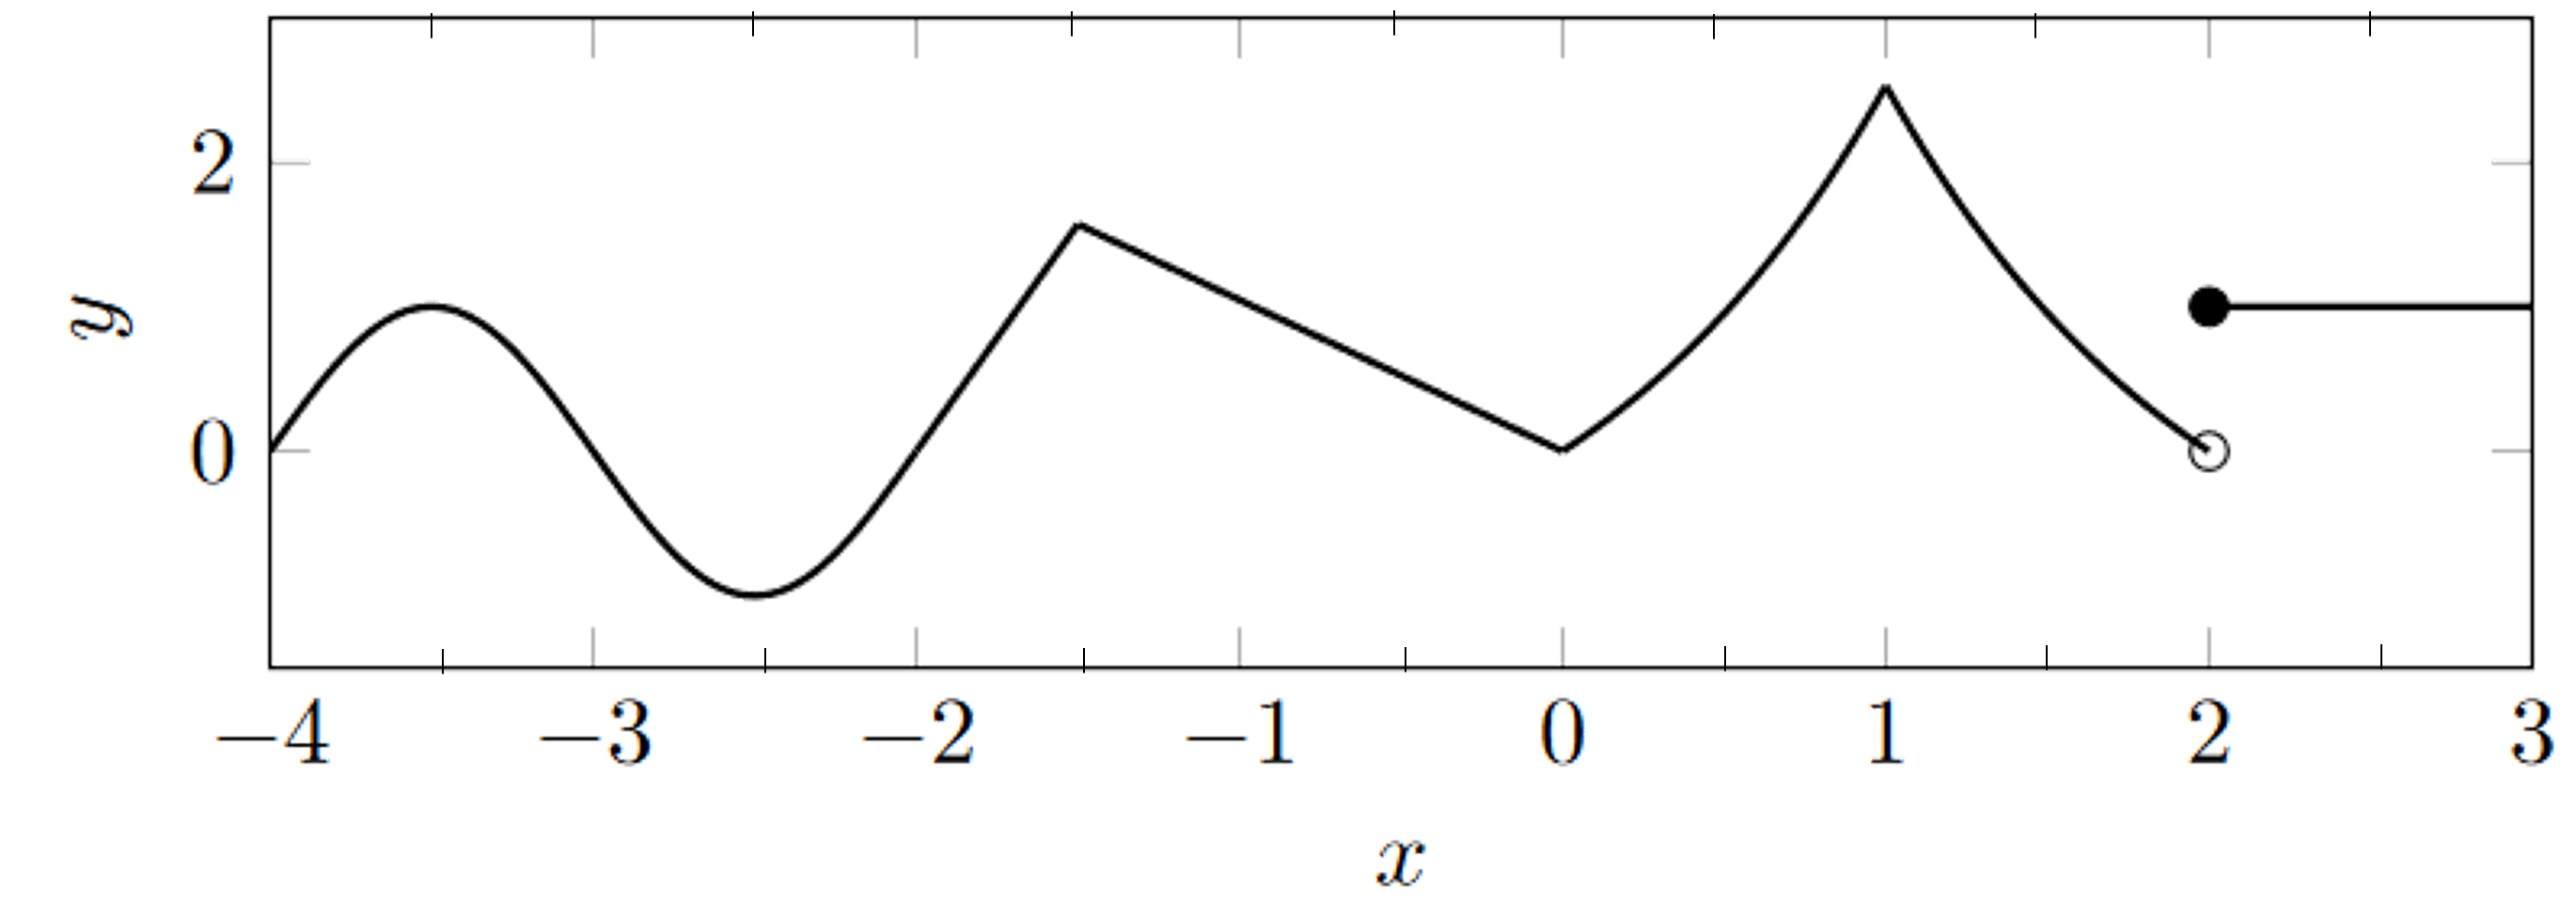
\includegraphics[width=0.75\textwidth]{../Mathematik_1/Bilder/ableitung_graphisch_skizzieren_aufgabe.png}
\end{center}

\vspace{0.3cm}
\noindent\textbf{L�sung:}\newline
	\begin{center}
	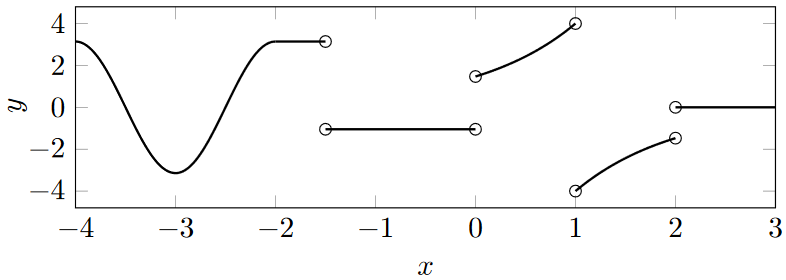
\includegraphics[width=0.75\textwidth]{../Mathematik_1/Bilder/ableitung_graphisch_skizzieren_loesung.png}
\end{center}
\end{exercisebox} 

\begin{exercisebox}[Differenzieren]
	Berechnen Sie von den folgenden Funktionen die Ableitungen. Es ist $a\in \mathbb R$ ein Parameter.
	\begin{eqnarray*}
		\begin{array}{ll}
			(a)\; f(x) = \mathrm{cosh}(x) = \displaystyle{\frac{e^x + e^{-x}}{2}} &\quad (b)\; g(u) = \displaystyle{\frac{u^2}{u^2+a^2}} \\[2ex]
			(c)\; h(p) = \mathrm{exp}\left(-p^2/(2a)^2\right) &\quad (d)\; i(x) = \displaystyle{\frac{(2x+3)^2-2}{\sqrt{x-1}}} \\
		\end{array}
	\end{eqnarray*}

	\vspace{0.3cm}
\noindent\textbf{L�sung:}
\begin{itemize}
	\item[(a)] $f'(x) = \displaystyle{\frac{e^x - e^{-x}}{2}} = \mathrm{sinh}(x)$
	\item[(b)] $g'(u) = \displaystyle{\frac{2a^2 u}{(u^2+a^2)^2}}$
	\item[(c)] $h'(p) = \displaystyle{-\frac{p}{2 \cdot a^2}} \cdot \mathrm{exp}\left( -p^2/(2\cdot a)^2\right)$
\item[(d)] $i'(x) = \displaystyle{ \frac{4(2x+3)}{\sqrt{x} - 1 }} - \displaystyle{ \frac{(2x+3)^2 - 2 }{2(x-1)^{3/2} }}$
	\end{itemize}
\end{exercisebox}

\begin{exercisebox}[Anwendungen: Monotonie-Satz]
Angenommen Sie wissen �ber eine Funktion $f$, dass ihre Ableitung auf einem Intervall $I$ negativ ist, also $f'(x) \leq 0$. Was k�nnen Sie dann �ber das Monotonie-Verhalten aussagen?

\vspace{0.3cm}
\noindent\textbf{L�sung:}\newline
$f$ ist auf $I$ monoton fallend. Es gelten die folgenden Monotonies�tze:
\begin{enumerate}
	\item $\forall x \in I: \; f'(x) = 0 \Leftrightarrow \, f$ ist konstant.
	\item $\forall x \in I: \; f'(x) \geq 0 \Leftrightarrow \, f$ monoton wachsend.
	\item $\forall x \in I: \; f'(x) \leq 0 \Leftrightarrow \, f$ monoton fallend.
	\item $\forall x \in I: \; f'(x) > 0 \Rightarrow \, f$  streng mononton wachsend.
	\item $\forall x \in I: \; f'(x) < 0 \Rightarrow \, f$  streng mononton fallend.
\end{enumerate}
\end{exercisebox}

\begin{exercisebox}[Anwendungen: Lineare N�herung]
      Die Mittellinie einer Rennstrecke der Breite $2\, \mathrm{m}$ wird durch Funktion $x\mapsto 4-\frac12 x^2$ beschrieben. Wir beobachten einen Rennwagen der die Bahnkurve im Uhrzeigersinn entlang rast. Bei spiegelglatter Fahrbahn rutscht das Fahrzeug und landet im Punkt $Y(0|6)$ in den Strohballen. Wo hat das Fahrzeug die Stra�e verlassen? 

\vspace{0.3cm}
\noindent\textbf{L�sung:}\newline
er Rennwagen verl�sst seine Bahn in einem bestimmten Punkt in tangentialer Richtung. Er bewegt sich anschlie�end in etwa geradlinig fort und landet im Punkt $Y(0|6)$ in den Strohballen. Eine Zeichnung l�sst vermuten, dass  $Y(0|6)$ auf der Tangente liegt, die die Bahnkurve im Punkt $B(-2|2)$ schneidet. Diese Tangente hat die Gleichung
\[ y = m x + b \; \textnormal{mit}\; m = f'(-2) = \frac{6-2}{0-(-2)} \land b = 6 \,.\]

      Der Punkt, in dem der Rennwagen die Stra�e verl�sst ist also der Schnittpunkt der Randkurve der Stra�e mit der Tangente am Punkt $B(-2|2)$. Die Gleichung der Randkurve ist \[ y=5-\frac12 x^2\] und damit erh�lt man 
      \[ 5-\frac12 x^2 = 2x + 6 \Leftrightarrow x_{1,2} = \frac{-4 \pm \sqrt{8}}{2}\,.\] Gesucht ist der Punkt $( \frac{-4 + \sqrt{8}}{2}| 2+\sqrt{8})$.
\end{exercisebox} 
 \newpage 
\setcounter{exercise}{0}\pagestyle{empty} \section*{Lokale Linearit�t L�sungen}\label{MA1-lokale-linearitaet-loesungen}

\ifintegriereaufgaben
	Regeln und Beispiele, die zum Verst�ndnis der L�sungswege hilfreich sind, finden Sie im Skript\wennreferenzvorhanden{MA1-lokale-linearitaet}{ (Abschnitt \abschnittsverweis{MA1-lokale-linearitaet})}.
\else
	Regeln und Beispiele, die zum Verst�ndnis der L�sungswege hilfreich sind, finden Sie im Skript.
\fi 

\begin{exercisebox}[Zentrale Differenz und zweite Differenz]
	\begin{itemize}
		\item[(a)] Zeigen Sie, dass sich die erste Ableitung von Polynomen vom Grad $2$ mit der zentralen Differenz exakt berechnen l��t.
		\item[(b)] Zeigen Sie, dass sich die zweite Ableitung von Polynomen vom Grad $4$ mit der zweiten Differenz exakt berechnen l��t.
	\end{itemize}

\hspace{0.3cm}
\newline
\textbf{L�sung:}
	\begin{itemize}
		\item[(a)] 
			Ein Polynom zweiten Grades mit Koeffizienten $a,b,c\in\mathbb R, \; a\not=0$ gilt 
			\[ p(x) = ax^2 + bx + c\; \Rightarrow p'(x) = 2ax + b \,.\] 
			Zu zeigen ist, dass die zentrale Differenz die erste Ableitung exakt approximiert. Betrachten wir beispielsweise die Ableitung an der Stelle $x_0 \in \mathbb R$. Es gilt f�r jedes $h>0$ 
			\begin{eqnarray*}
				\frac{ p(x_0+h) - p(x_0-h)}{2h} &=&  
				\frac{ a(x_0+h)^2+b(x_0+h) +c - \left( a(x_0-h)^2+b(x_0-h) +c\right) }{2h} \\   
				&=& \frac{ 4 ahx_0 + 2 h b }{2h}= ax + b = p'(x_0) \,.   
			\end{eqnarray*}
		\item[(b)]
			Ein Polynom dritten Grades mit Koeffizienten $a,b,c,d\in\mathbb R, \; a\not=0$ gilt 
			\[ p(x) = ax^3 + bx^2 + cx + d\; \Rightarrow p''(x) = 6ax + 2b \,.\] 
			Zu zeigen ist, dass die zweite Differenz die zweite Ableitung exakt approximiert. Betrachten wir beispielsweise die zweite Ableitung an der Stelle $x_0 \in \mathbb R$. Es gilt f�r jedes $h>0$ 
			\begin{eqnarray*}
			&& \frac{ p(x_0+h) - 2 p(x_0) + p(x_0-h)}{h^2} \\
			&=& =  \frac{ a(x_0+h)^3+b(x_0+h)^2 +c(x_0+h) + d }{h^2} \\
			&& - 2 \frac{\left(ax_0^3+bx_0^2 +cx_0 + d  \right)}{h^2} +\frac{a(x_0-h)^3+b(x_0-h)^2 +c(x_0-h) + d }{h^2} \\
		&=&   a\frac{ ( x^3 + 3 h x^2 + 3 h^2 x + h^3) - 2 x^3 + ( x^3 - 3 hx^2 + 3 h^2 x -h^3)}{h^2} \\
		&& + b \frac{  ( x^2 + 2 h  + h^2 )  - b x^2 + (x^2 - 2 h + h^2 )  }{h^2} \\ 
				&=& \frac{  6 a  h^2 x  + 2 b h^2  }{h^2}=  6 a x + 2 b \,.  
			\end{eqnarray*}
	\end{itemize}
\end{exercisebox}

\begin{exercisebox}[Bestapproximation]
	Gegeben seien Messungen $x_1, x_2, \cdots, x_n\in\mathbb R$, $n\in \mathbb N$ einer Gr��e $x\in \mathbb R$. Gesucht ist eine Approximation $\tilde x\in \mathbb R$, deren Abstand zu allen Messwerten gleichzeitig minimal ist, also 
	\[ \sum\limits_{k=1}^n |x- x_k|^2 \stackrel{!}{=} \mathrm{min}\,.\]
		Bestimmen Sie eine Formel f�r $\tilde x$. 


\hspace{0.3cm}
\newline
\textbf{L�sung:}
Fassen wir den Term auf der rechten Seite als Funktion von $x$ auf, dann ist das Minimum dieser Funktion gesucht. Um das Minimum zu bestimmen, suchen wir zun�chst kritische Punkte und �berpr�fen diese mittels der zweiten Ableitung. 
Bei der Berechnung der ersten Ableitung muss man sich dar�ber Klarheit verschaffen, wie die Ableitung der Betragsfunktion funktioniert:
Damit gilt
\begin{eqnarray*} 
	Q'(x) = \sum\limits_{k=1}^n 2 \cdot (x-x_k)\,. \\
	Q''(x) = \sum\limits_{k=1}^n 2 = 2n > 0 \textnormal{ f"ur alle } x\in\mathbb R\,.
\end{eqnarray*}
Nun bestimmen wir die Nullstellen der ersten Ableitung:
\[ Q'(x) = 0 \Leftrightarrow \sum\limits_{k=1}^n -2\cdot (x-x_k) = 0 \Leftrightarrow 2 n x = -2\sum\limits_{k=1}^n x_k\,.\] 
Also ist die beste Approximation an alle Messpunkte gerade ihr arithmetisches Mittel: \[ \tilde x = -\frac1n \cdot \sum\limits_{k=^n} x_k\,. \]
\end{exercisebox} 

\begin{exercisebox}[Taylorentwicklung]
	Gegeben sei die Funktion $f: x\mapsto \cos(x)$. Bestimmen Sie die Taylorentwicklung $T_7$ von $f$ an der Stelle $x_0=0$ und sch�tzen Sie den Betrag des Lagrangeschen Restglieds $R_8$ im Intervall $x\in I= [ -\pi/6, \pi/6]$ ab. 

  \hspace{0.3cm}
  \newline
  \textbf{L�sung:}
  Es gilt 
  \[ \begin{array}{rcl rcl }
		  f(x) &=& \cos(x), & f(0) &=& 1 \\
		  f'(x) &=& -\sin(x), & f'(0) &=& 0 \\
		  f''(x) &=& -\cos(x), & f''(0) &=& -1 \\
		  f''(x) &=& \sin(x), & f''(0) &=& 0 \\
		  f^{(4)}(x) &=& \cos(x), & f^{(4)}(0) &=& 1 \\
		  f^{(5)}(x) &=& -\sin(x), & f^{(5)}(0) &=& 0 \\
		  f^{(6)}(x) &=& -\cos(x), & f^{(6)}(0) &=& -1 \\
		  f^{(7)}(x) &=& \sin(x), & f^{(7)}(0) &=& 1 \\
		  f^{(8)}(x) &=& \cos(x), & |f^{(8)}(x)| &=& \leq 1
	  \end{array}
  \]
  Damit folgt \[ T_7(x) = 1 -\frac12 x^2 + \frac{1}{24} x^4 - \frac{1}{720} x^6 \quad \textnormal{und}\quad |R_8(x)| \leq \frac{ |\cos(\xi)|}{8!} \left( \pi/6\right)^8 = \frac{\pi^8}{6^8\cdot 8!} \approx 1.4\cdot 10^{-7} \,.\]
\end{exercisebox} 

\begin{exercisebox}[Interpolation (Wiederholung)]
Gegeben sind die Punkte 
\begin{center}
	\begin{tabular}{c|cccc}
		$i$ & $0$ & $1$ & $2$ & $3$ \\
		\hline
		$x_i$ & $-3$ & $-1$ & $0$ & $2$ \\
		\hline
		$y_i$ & $-3$ & $1$ & $0$ & $82$ \\
	\end{tabular}
\end{center}
\begin{itemize}
	\item[(a)]  Bestimmen Sie den Grad $n$ des Interpolationspolynoms. 
	\item[(b)]  Bestimmen Sie das lineare Gleichungssystem f�r die Koeffizienten des Interpolationspolynoms in der Darstellung \[ p(x) =a_nx^n+\cdots +a_1 x+a_0\] und l�sen Sie es.
	%\item[(c)]  Bestimmen Sie den Wert des Polynoms an der Zwischenstelle $\tilde x= 1$.
	%\item[(d)]  Bestimmen Sie das lineare Gleichungssystem f�r die Koeffizienten des Interpolationspolynoms in der Darstellung \[ q(x) =c_0+c_1(x-x_0) +c_2(x-x_0)(x-x_1) +\cdots +c_n(x-x_0)\cdots(x-x_{n-1})\] und l�sen Sie es mit Matlab.
	%\item[(e)]  Berechnen Sie den Wert des Polynoms $q$ an der Zwischenstelle $\tilde x= 1$. Wie k�nnnen Sie den Wert effizient berechnen?
\end{itemize}

\hspace{0.3cm}
\newline
\textbf{L�sung:}
\begin{itemize}
	\item[(a)] Da vier Punkte zu interpolieren sind, hat das Polynom den Grad drei \[ p: x \mapsto a_3 x^3 + a_2 x^2 + a_2 x^1 + a_0\,.\] 
	\item[(b)] Die Bedingungen $p(x_i) = y_i$ f�r $i=1,2,3,4$ f�hren auf das folgende lineare Gleichungssystem:
		\[ \left( \begin{array}{cccc} -27 & 9 & -3 & 1 \\ -1 & 1 & -1 & 1 \\ 0 & 0 & 0 & 1 \\ 8 & 4 & 2 &1 \end{array}\right) \cdot \left( \begin{array}{c} a_3 \\ a_2 \\ a_1 \\ a_0 \end{array}\right) = \left( \begin{array}{c} -3 \\ 1 \\ 0 \\82 \end{array}\right)\,. \]
		Die L�sung lautet $a_3=3, \, a_2 = 11,\, a_1 = 7, \, a_0 = 0$ und damit \[ p:x\mapsto 3x^3 + 11 x^2 + 7 x \,,.\]
	\end{itemize}
\end{exercisebox}

\begin{exercisebox}[Interpolation (Wiederholung)]
	Eine Funktion der Form \[ f: x \mapsto \frac{a_0}{2} + a_1 \cos(x) + b_1 \sin(x) \,,\] soll durch die Punkte $(x_i, y_i), i=1,2,3$ mit \[ (0|1), \, (\pi/6|-1),\, (\pi/2|-3)\] gelegt werden. Bestimmen Sie ein Gleichungssystem f�r die Koeffizienten $a_0, a_1, b_1$ und l�sen Sie es.

\hspace{0.3cm}
\newline
\textbf{L�sung:}
Allgmein muss gelten 
\[\left(\begin{array}{ccc} \frac12 & \cos(x_1) & \sin(x_1) \\\frac12 & \cos(x_2) & \sin(x_2) \\  \frac12 & \cos(x_3) & \sin(x_3) \end{array}\right) \cdot \left( \begin{array}{c} a_0 \\ a_1 \\ b_1 \end{array}\right) = \left( \begin{array}{c} y_1 \\ y_2 \\ y_3 \end{array}\right) \]
F�r die gegebenen Punkte lautet das Gleichungssystem also konkret
\[\left(\begin{array}{ccc} \frac12 & 1 & 0 \\\frac12 & \frac{\sqrt{3}}{2} & \frac12 \\  \frac12 & 0 & 1 \end{array}\right) \cdot \left( \begin{array}{c} a_0 \\ a_1 \\ b_1 \end{array}\right) = \left( \begin{array}{c} 1 \\ -1 \\ -3 \end{array}\right) \]
Die L�sung lautet $a_0 = 2, \, a_1 = 0,\, b_1 = -4 \,. $ und damit $f:x\mapsto 1-4 \sin(x)\,.$
\end{exercisebox} 
 \newpage 
\setcounter{exercise}{0}\pagestyle{empty} \section*{Kurvendiskussion L�sungen}\label{MA1-ableitungen-und-funktionsverlauf-loesungen}

\ifintegriereaufgaben
	Regeln und Beispiele, die zum Verst�ndnis der L�sungswege hilfreich sind, finden Sie im Skript\wennreferenzvorhanden{MA1-ableitungen-und-funktionsverlauf}{ (Abschnitt \abschnittsverweis{MA1-ableitungen-und-funktionsverlauf})}.
\else
	Regeln und Beispiele, die zum Verst�ndnis der L�sungswege hilfreich sind, finden Sie im Skript.
\fi 

\begin{exercisebox}[Grenzwerte mit L'Hospital] %Andreas
	Berechnen Sie die folgenden Grenzwerte mit der Regel von L'Hospital. %Hinweis zu $(d)$: Untersuchen Sie $\log$\dots
	\begin{eqnarray*}
		(a)\; \displaystyle{\lim\limits_{x\to 0}}\; \displaystyle{\frac{\sin(\sin(x))}{x}}  \quad\quad  (b)\; \displaystyle{\lim\limits_{x\to \infty}}\;\displaystyle{x^2 \cdot 2^{-x}}  \quad\quad\quad\quad (c)\; \displaystyle{\lim\limits_{x\downarrow 0}}\; x \cdot \ln(x) 
	\end{eqnarray*}

\vspace{0.3cm}
\noindent\textbf{L�sung:}\newline
\begin{itemize}
	\item[(a)] 
		Die Regel ist anwendbar, da 
		\begin{eqnarray*}
			\begin{cases} \displaystyle{\lim\limits_{x\to 0}} \sin(\sin(x)) = \sin(\sin(0)) = 0 \\  \displaystyle{\lim\limits_{x\to 0}} x = 0 \,. \end{cases} 
		\end{eqnarray*}
		Die Ableitungen von Z�hler und Nenner lauten 
		\begin{eqnarray*}
			\begin{cases} \left( \sin(\sin(x))\right)' = \cos(\sin(x)) \cdot \cos(x) \\   \left( x \right)' = 1  \,. \end{cases} 
		\end{eqnarray*}
		Der Grenzwert 
		\begin{eqnarray*}
			\lim\limits_{x\to 0 } \frac{\cos(\sin(x)) \cdot \cos(x) }{1} = \frac{\cos(\sin(0))}{1} = 1 
		\end{eqnarray*}
		existiert und mit L'Hospital folgt 
		\[ \lim\limits_{x\to 0} \frac{\sin(\sin(x))}{x} = 1 \,.\]
	\item[(b)]
		Die Regel ist anwendbar, da 
		\begin{eqnarray*}
			\displaystyle{\lim\limits_{x\to \infty}} x^2\cdot 2^{-x} = \displaystyle{\lim\limits_{x\to \infty}} \frac{x^2}{ 2^{x}}  \textnormal{ mit }  
			\begin{cases} 
				\displaystyle{\lim\limits_{x\to \infty}} x^2 = \infty  \\  \displaystyle{\lim\limits_{x\to \infty}} 2^x = \infty \,. \end{cases} 
		\end{eqnarray*}
		Die Ableitungen von Z�hler und Nenner lauten 
		\begin{eqnarray*}
			\begin{cases} 
				\left( x^2 \right)' = 2 x \\  \left( 2^x \right)' = \left( \exp(x\cdot \ln(2) \right)' = \ln(2) \cdot 2^x  \,. \end{cases} 
		\end{eqnarray*}
		Es zeigt sich, dass auch der Grenzwert der ersten Ableitungen vom Typ "$\infty/\infty$" ist. Deswegen betrachten wir die zweiten Ableitungen. 
		\begin{eqnarray*}
			\begin{cases} 
				\left( x^2 \right)'' = 2 \\  \left( 2^x \right)'' = \ln(2)^2 \cdot 2^x  \,. \end{cases} 
		\end{eqnarray*}
		Der Grenzwert 
		\begin{eqnarray*}
			\lim\limits_{x\to \infty } \frac{2 }{(\ln(2)^2\cdot 2^x} = 0 
		\end{eqnarray*}
		existiert und mit L'Hospital folgt 
		\[ \lim\limits_{x\to \infty} x^2 \cdot 2^{-x}= 0 \,.\]
	\item[(c)] 
		Der Grenzwert ist �quivalent zu 
		\[ \lim\limits_{x\downarrow 0} x \cdot \ln(x) = -\lim\limits_{x\downarrow 0} \frac{-\ln(x)}{\frac1x} \]
		mit den Grenzwerten
		\begin{eqnarray*}
			\begin{cases} \displaystyle{\lim\limits_{x\downarrow 0}} (-\ln(x))  =  \infty   \\  \displaystyle{\lim\limits_{x\downarrow 0}} \displaystyle{\frac1x} = \infty \,. \end{cases} 
		\end{eqnarray*}
		Die Regel ist anwendbar und wir berechnen die  Ableitungen von Z�hler und Nenner 
		\begin{eqnarray*}
			\begin{cases} \left(-\ln(x)\right)' = -\displaystyle{\frac1x} \\   \left( \displaystyle{\frac1x} \right)' = -\displaystyle{\frac{1}{x^2}}  \,. \end{cases} 
		\end{eqnarray*}
		Der Grenzwert 
		\begin{eqnarray*}
			\lim\limits_{x\downarrow 0 } \frac{-1/x  }{ - 1/x^2} = 0 
		\end{eqnarray*}
		existiert und mit L'Hospital folgt 
		\[ \lim\limits_{x\downarrow 0} x\cdot \ln(x)  = 0 \,.\]
\end{itemize}
\end{exercisebox}

\begin{exercisebox}[Extremwerte] %p. 103 LS
    Zerlegen Sie die Zahl $12$ so in zwei Summanden, dass ihr Produkt m�glichst gro� wird. 

\vspace{0.3cm}
\noindent\textbf{L�sung:}\newline
			Gesucht sind Zahlen \(x,y\in\mathbb R\), so dass \( x+y=12\) und gleichzeitig \(x\cdot y = \mathrm{min}\). Aus der ersten Gleichung folgt \(y = 12-x\) und damit suchen wir ein Minimum der Funktion \(f:x\mapsto x\cdot (1-x)\):   
			\[ f(x) = x\cdot (12 - x ) \Rightarrow f'(x_0) \stackrel{!}{=}0 \Leftrightarrow = 12-2\cdot x = 0 \Leftrightarrow x = 6 \land f''(6) = 12 > 0 \Rightarrow \textnormal{ Minimum} \] 
Die Antwort ist \(x=y=6\).

\end{exercisebox} 

\begin{exercisebox}[Abbildungsvorschrift] %p. 111 LS
	Begr�nden Sie, warum es keine ganzrationale Funktion $f$ gibt mit folgenden Eigenschaften: $f$ hat Grad $2$, $f$ hat Nullstellen f�r $x=2$ und $x=4$ und ein Maximum f�r $x=0$.

\vspace{0.3cm}
\noindent\textbf{L�sung:}\newline
\[ f:x\mapsto c \cdot (x-2)\cdot (x-4) \Rightarrow f(x) = c (x^2 - 6 \cdot x + 8) \Rightarrow f'(x) = 2 \cdot c\cdot (x-3) = 0 \Leftrightarrow x = 3 \land f''(3) \not=0\] Das hei�t, dass $f$ eine Extremstelle nur an der STelle $x=3$ haben kann und nicht f�r $x=0$.   
\end{exercisebox} 

\begin{exercisebox}[Extrema] %p131 LS
  Es sei $f=u\circ v$ und die Funktionen $u,v$ und $f$ seien auf $\mathbb R$ differenzierbar. Beweisen oder widerlegen Sie die Aussage:
  \begin{itemize}
	  \item[(a)] Ist $x_0$ eine Extremstelle von $f$, dann ist $x_0$ auch eine Extremstelle von $v$
    \item[(b)] Ist $x_0$ eine Extremstelle von $v$, dann ist $x_0$ auch eine Extremstelle von $f$
  \end{itemize}

\vspace{0.3cm}
\noindent\textbf{L�sung:}\newline
F�r die Ableitung der verketteten Funktion gilt $f': x \mapsto u'(v(x)) \cdot v'(x)$
\begin{itemize}
	\item[(a)] $f'(x_0) = 0 \Leftrightarrow  u'(v(x_0)) = 0 \lor v'(x_0) \quad  \Rightarrow $ die Aussage unter $(a)$ ist falsch (Bsp. $f(x) = (\sin(x))^2$).
	\item[(b)] $v'(x_0) = 0 \Rightarrow  u'(v(x_0)) \cdot v'(x_0) = f'(x_0) = 0 \quad  \Rightarrow  x_0$ ist ein kritischer Punkt von $f$. Zus�tzlich wissen wir, dass $v'$ an der Stelle $x_0$ einen Vorzeichenwechsel hat. Also hat auch $f'$ an der Stelle $x_0$ einen Vorzeichenwechsel und damit ist $x_0$ auch eine Extremstelle von $f$. Die Aussage unter $(b)$ ist wahr.
\end{itemize}
\end{exercisebox}

\begin{exercisebox}[Wendepunkte] %p133 LS
  Bei einer Funktion $f$ gelte f�r alle $x\in \mathbb R: f(x)\not = 0$. $f$ ist differenzierbar udn $f'(x) = x\cdot f(x)$.
  \begin{itemize}
	  \item[(a)] Stellen Sie $f''(x)$ und $f'''(x)$ durch $f(x)$ dar.
    \item[(b)] Zeigen Sie, dass $f$ an der Stelle $0$ ein lokales Extremum hat. Welche Bedingung muss $f$ erf�llen, dass es sich um ein Maximum handelt?
    \item[(c)] Begr�nden Sie, dass $f$ keine Wendestelle besitzt.
  \end{itemize}

\vspace{0.3cm}
\noindent\textbf{L�sung:}\newline
\begin{itemize}
	\item[(a)] \begin{eqnarray*}
			f''(x) &=& f(x) + x\cdot f'(x) = f(x) \cdot (1+x^2) \\ 
			f'''(x) &=& x \cdot f(x) \cdot (3 + x^2) 
		\end{eqnarray*}
	\item[(b)] $x_0 = 0$ ist ein kritischer Punkt von $f$, da  $f'(0) = 0\cdot f(0) = 0$. Au�erdem gilt $f''(0) = f(0) \not=0$ laut Voraussetzung, also liegt an der Stelle $x_0=0$ ein lokales Extremmum vor. Es handelt sich um ein Maximum, wenn $f(0) < 0$ ist.  
	\item[(c)] Die notwendige Bedingung luatet $f''(x) = 0$. Da $f''(x) \not= 0$ f�r alle $x\in \mathbb R$, hat $f$ keine Wendestelle.
\end{itemize}
\end{exercisebox} 

\begin{exercisebox}[Kurvendiskussion]
	F�hren Sie f�r die Funktion $f$ eine Kurvendiskussion durch: \[ f: x\mapsto \frac{x^3}{x^2-1}\] %Bestimmen Sie den Definitionsbereich das Symmetrieverhalten, die Nullstellen, das Verhalten an etwaigen Polstellen, das asymptotische Verhalten f�r $|x| \to \infty$, Extremwerte, Wendepunkte und den Bildbereich. Skizzieren Sie die dann die Funktion. 

\vspace{0.3cm}
\noindent\textbf{L�sung:}\newline
Die  ersten zwei Ableitungen von $f$ lauten: 
\begin{eqnarray*}
	f'(x) &=& \frac{x^4-3\cdot x^2}{(x^2-1)^2} \\
	f''(x) &=& \frac{2\,x\cdot (x^2+3)}{(x^2-1)^3}
\end{eqnarray*} 
\begin{enumerate}
	\item (Definitionsbereich) $f$ ist �berall definiert, wo der Nenner null wird, also \[ x^2-1 = 0 \Leftrightarrow x=\pm 1 \Rightarrow D_f = \mathbb R \setminus\{-1,1\} \,.\]
	\item (Symmetrie) $f$ ist ungerade, denn \[ f(-x) = \frac{(-x)^3}{(-x)^2-1} = - \frac{x^3}{x^2-1} = -f(x)\,.\]
	\item (Nullstellen) $f$ hat eine dreifache Nullstelle f�r $x=0$, denn 
		\[ f(x) = 0 \Leftrightarrow x^3 = 0 \Leftrightarrow x=0\,.\]
	\item (Polstellen) $f$ hat in $x=\pm 1$ jeweils eine Polstelle mit Vorzeichenwechsel, denn 
		\begin{eqnarray*}
			\lim\limits_{x\downarrow 1 } \frac{x^3}{x^2-1} = \infty \land \lim\limits_{x\uparrow 1 } \frac{x^3}{x^2-1} = -\infty\,, \\
			\lim\limits_{x\downarrow -1 } \frac{x^3}{x^2-1} = -\infty \land \lim\limits_{x\uparrow -1 } \frac{x^3}{x^2-1} = \infty\,.
		\end{eqnarray*}
	\item (Waagerechte Asymptoten) Die Grenzwerte f�r $|x|\to \infty$ ergeben sich zu 
		\[ \lim\limits_{x\to \infty}\frac{x^3}{x^2-1} =  \lim\limits_{x\to \infty} x \frac{1}{1-1/x^2} = \infty \land \lim\limits_{x\to -\infty}\frac{x^3}{x^2-1} = - \infty\,. \]
	\item (Extremstellen) $f$ hat ein lokales Minium bei $(\sqrt{3}|3\sqrt{3}/2)$ und ein lokales Maximum bei $(-\sqrt{3}, -3\sqrt{3}/2)$, denn 
		\begin{itemize}
			\item[(a)] Kandidaten f�r Extremstellen \[ f'(x) = 0 \Leftrightarrow \frac{x^4-3x^2}{(x^2-1)^2} = 0 \Leftrightarrow x^2(x^2-3) = 0 \Leftrightarrow x \in \{ -\sqrt{3}, 0, \sqrt{3}\}\,.\]
				\item[(b)] Analyse der Kandidaten mit Hilfe der zweiten Ableitung 
					\begin{eqnarray*}
						f''(0) &=& 0 \Rightarrow \textnormal{ keine Entscheidung m�glich}\,,\\
						f''(-\sqrt{3}) &=& -3\sqrt{3}/2 \Rightarrow \textnormal{ lokales Minimum}\,,\\
						f''(\sqrt{3}) &=& 3\sqrt{3}/2 \Rightarrow \textnormal{ lokales Maximum}\,.
					\end{eqnarray*}
					F�r $x=0$ kann man entweder die dritte Ableitung anschauen oder pr�fen, ob die zweite Ableitung einen Vorzeichenwechsel hat beim �bergang von $x=-h$ zu $x=h$. $f''$ hat keinen Vorzeichenwechsel an der Stelle $x=0$, denn \[  f''(x) = \frac{x^2\cdot (x^2-3)}{(x^2-1)^2} < 0 \quad x\in(-\sqrt{3},\sqrt{3}) \setminus\{0\} \] und damit ist $x=0$ keine Extremstelle.
       		\end{itemize}
				\item (Wendestellen) Kandidaten f�r Wendestellen sind die kritischen Puntke der zweiten Ableitung, also \[ f''(x) = 0 \Leftrightarrow \frac{2x(x^2+3)}{(x^2-1)^2} = 0\,, \] das hei�t im Definitionsbereich nur f�r $x=0$. Die zweite Ableitung �ndert dort ihr Vorzeichen, also liegt in $(0|0) $ ein Wendepunkt vor.
				\item (Bildbereich) Der Bildbereich ist $\mathbb R$.
			\end{enumerate}
\end{exercisebox}

\begin{exercisebox}[Anwendungen: Newton-Verfahren] %Andreas
	Gegeben ist die Funktion 
	\[ f:\mathbb R \to \mathbb R, \; x\mapsto f(x) = e^{-x} - \sin(x)\]
	und $x_0 = 0$. Gesucht ist eine Nullstelle $\tilde x $ der Funktion f. 
	\begin{itemize}
		\item[(a)] Bestimmen Sie die lineare Approximation $t(x) = mx+b$ an der Stelle $x_0$.
		\item[(b)] Stellen Sie die Iterationsvorschrift f�r das Newtonverfahren auf.
		\item[(c)] Berechnen Sie die ersten Iterierten des Newton-Verfahrens und geben Sie eine Sch�tzung f�r die L�sung an.
	\end{itemize}
\noindent\textbf{L�sung:}\newline
\begin{itemize}
	\item[(a)] Es ist  
		\[ f'(x) = -e^{-x} - \cos(x), \; f'(x_0) = f'(0) = -2\] 
		und damit lautet die Tangentengleichung 
		\[ t(x) = f'(x_0) (x-x_0) + f(x_0) = (-2) x (x-0) +1 = 1-2x\,.\] 
	\item[(b)] Es gilt 
		\[ x_{k+1} = x_k - \frac{e^{-x_k} - \sin(x_k) }{-e^{-x_k} - \cos(x_k)}\,.\]
		\item[(c)] Eine N�herung f�r die Nullstelle ist $\tilde x \approx 0.58853274398 $.
	\end{itemize}
\end{exercisebox}
 \newpage 
}

\end{document}
